% Options for packages loaded elsewhere
\PassOptionsToPackage{unicode}{hyperref}
\PassOptionsToPackage{hyphens}{url}
%
\documentclass[
  10pt,
  b5paper,
  oneside]{book}
\usepackage{amsmath,amssymb}
\usepackage{iftex}
\ifPDFTeX
  \usepackage[T1]{fontenc}
  \usepackage[utf8]{inputenc}
  \usepackage{textcomp} % provide euro and other symbols
\else % if luatex or xetex
  \usepackage{unicode-math} % this also loads fontspec
  \defaultfontfeatures{Scale=MatchLowercase}
  \defaultfontfeatures[\rmfamily]{Ligatures=TeX,Scale=1}
\fi
\usepackage{lmodern}
\ifPDFTeX\else
  % xetex/luatex font selection
\fi
% Use upquote if available, for straight quotes in verbatim environments
\IfFileExists{upquote.sty}{\usepackage{upquote}}{}
\IfFileExists{microtype.sty}{% use microtype if available
  \usepackage[]{microtype}
  \UseMicrotypeSet[protrusion]{basicmath} % disable protrusion for tt fonts
}{}
\makeatletter
\@ifundefined{KOMAClassName}{% if non-KOMA class
  \IfFileExists{parskip.sty}{%
    \usepackage{parskip}
  }{% else
    \setlength{\parindent}{0pt}
    \setlength{\parskip}{6pt plus 2pt minus 1pt}}
}{% if KOMA class
  \KOMAoptions{parskip=half}}
\makeatother
\usepackage{xcolor}
\usepackage{color}
\usepackage{fancyvrb}
\newcommand{\VerbBar}{|}
\newcommand{\VERB}{\Verb[commandchars=\\\{\}]}
\DefineVerbatimEnvironment{Highlighting}{Verbatim}{commandchars=\\\{\}}
% Add ',fontsize=\small' for more characters per line
\usepackage{framed}
\definecolor{shadecolor}{RGB}{248,248,248}
\newenvironment{Shaded}{\begin{snugshade}}{\end{snugshade}}
\newcommand{\AlertTok}[1]{\textcolor[rgb]{0.94,0.16,0.16}{#1}}
\newcommand{\AnnotationTok}[1]{\textcolor[rgb]{0.56,0.35,0.01}{\textbf{\textit{#1}}}}
\newcommand{\AttributeTok}[1]{\textcolor[rgb]{0.13,0.29,0.53}{#1}}
\newcommand{\BaseNTok}[1]{\textcolor[rgb]{0.00,0.00,0.81}{#1}}
\newcommand{\BuiltInTok}[1]{#1}
\newcommand{\CharTok}[1]{\textcolor[rgb]{0.31,0.60,0.02}{#1}}
\newcommand{\CommentTok}[1]{\textcolor[rgb]{0.56,0.35,0.01}{\textit{#1}}}
\newcommand{\CommentVarTok}[1]{\textcolor[rgb]{0.56,0.35,0.01}{\textbf{\textit{#1}}}}
\newcommand{\ConstantTok}[1]{\textcolor[rgb]{0.56,0.35,0.01}{#1}}
\newcommand{\ControlFlowTok}[1]{\textcolor[rgb]{0.13,0.29,0.53}{\textbf{#1}}}
\newcommand{\DataTypeTok}[1]{\textcolor[rgb]{0.13,0.29,0.53}{#1}}
\newcommand{\DecValTok}[1]{\textcolor[rgb]{0.00,0.00,0.81}{#1}}
\newcommand{\DocumentationTok}[1]{\textcolor[rgb]{0.56,0.35,0.01}{\textbf{\textit{#1}}}}
\newcommand{\ErrorTok}[1]{\textcolor[rgb]{0.64,0.00,0.00}{\textbf{#1}}}
\newcommand{\ExtensionTok}[1]{#1}
\newcommand{\FloatTok}[1]{\textcolor[rgb]{0.00,0.00,0.81}{#1}}
\newcommand{\FunctionTok}[1]{\textcolor[rgb]{0.13,0.29,0.53}{\textbf{#1}}}
\newcommand{\ImportTok}[1]{#1}
\newcommand{\InformationTok}[1]{\textcolor[rgb]{0.56,0.35,0.01}{\textbf{\textit{#1}}}}
\newcommand{\KeywordTok}[1]{\textcolor[rgb]{0.13,0.29,0.53}{\textbf{#1}}}
\newcommand{\NormalTok}[1]{#1}
\newcommand{\OperatorTok}[1]{\textcolor[rgb]{0.81,0.36,0.00}{\textbf{#1}}}
\newcommand{\OtherTok}[1]{\textcolor[rgb]{0.56,0.35,0.01}{#1}}
\newcommand{\PreprocessorTok}[1]{\textcolor[rgb]{0.56,0.35,0.01}{\textit{#1}}}
\newcommand{\RegionMarkerTok}[1]{#1}
\newcommand{\SpecialCharTok}[1]{\textcolor[rgb]{0.81,0.36,0.00}{\textbf{#1}}}
\newcommand{\SpecialStringTok}[1]{\textcolor[rgb]{0.31,0.60,0.02}{#1}}
\newcommand{\StringTok}[1]{\textcolor[rgb]{0.31,0.60,0.02}{#1}}
\newcommand{\VariableTok}[1]{\textcolor[rgb]{0.00,0.00,0.00}{#1}}
\newcommand{\VerbatimStringTok}[1]{\textcolor[rgb]{0.31,0.60,0.02}{#1}}
\newcommand{\WarningTok}[1]{\textcolor[rgb]{0.56,0.35,0.01}{\textbf{\textit{#1}}}}
\usepackage{longtable,booktabs,array}
\usepackage{calc} % for calculating minipage widths
% Correct order of tables after \paragraph or \subparagraph
\usepackage{etoolbox}
\makeatletter
\patchcmd\longtable{\par}{\if@noskipsec\mbox{}\fi\par}{}{}
\makeatother
% Allow footnotes in longtable head/foot
\IfFileExists{footnotehyper.sty}{\usepackage{footnotehyper}}{\usepackage{footnote}}
\makesavenoteenv{longtable}
\usepackage{graphicx}
\makeatletter
\newsavebox\pandoc@box
\newcommand*\pandocbounded[1]{% scales image to fit in text height/width
  \sbox\pandoc@box{#1}%
  \Gscale@div\@tempa{\textheight}{\dimexpr\ht\pandoc@box+\dp\pandoc@box\relax}%
  \Gscale@div\@tempb{\linewidth}{\wd\pandoc@box}%
  \ifdim\@tempb\p@<\@tempa\p@\let\@tempa\@tempb\fi% select the smaller of both
  \ifdim\@tempa\p@<\p@\scalebox{\@tempa}{\usebox\pandoc@box}%
  \else\usebox{\pandoc@box}%
  \fi%
}
% Set default figure placement to htbp
\def\fps@figure{htbp}
\makeatother
\ifLuaTeX
  \usepackage{luacolor}
  \usepackage[soul]{lua-ul}
\else
  \usepackage{soul}
\fi
\setlength{\emergencystretch}{3em} % prevent overfull lines
\providecommand{\tightlist}{%
  \setlength{\itemsep}{0pt}\setlength{\parskip}{0pt}}
\setcounter{secnumdepth}{5}
% definitions for citeproc citations
\NewDocumentCommand\citeproctext{}{}
\NewDocumentCommand\citeproc{mm}{%
  \begingroup\def\citeproctext{#2}\cite{#1}\endgroup}
\makeatletter
 % allow citations to break across lines
 \let\@cite@ofmt\@firstofone
 % avoid brackets around text for \cite:
 \def\@biblabel#1{}
 \def\@cite#1#2{{#1\if@tempswa , #2\fi}}
\makeatother
\newlength{\cslhangindent}
\setlength{\cslhangindent}{1.5em}
\newlength{\csllabelwidth}
\setlength{\csllabelwidth}{3em}
\newenvironment{CSLReferences}[2] % #1 hanging-indent, #2 entry-spacing
 {\begin{list}{}{%
  \setlength{\itemindent}{0pt}
  \setlength{\leftmargin}{0pt}
  \setlength{\parsep}{0pt}
  % turn on hanging indent if param 1 is 1
  \ifodd #1
   \setlength{\leftmargin}{\cslhangindent}
   \setlength{\itemindent}{-1\cslhangindent}
  \fi
  % set entry spacing
  \setlength{\itemsep}{#2\baselineskip}}}
 {\end{list}}
\usepackage{calc}
\newcommand{\CSLBlock}[1]{\hfill\break\parbox[t]{\linewidth}{\strut\ignorespaces#1\strut}}
\newcommand{\CSLLeftMargin}[1]{\parbox[t]{\csllabelwidth}{\strut#1\strut}}
\newcommand{\CSLRightInline}[1]{\parbox[t]{\linewidth - \csllabelwidth}{\strut#1\strut}}
\newcommand{\CSLIndent}[1]{\hspace{\cslhangindent}#1}
\usepackage{booktabs}
\usepackage{amsthm}
\makeatletter
\let\stdl@chapter\l@chapter
\renewcommand*{\l@chapter}[2]{%
  \stdl@chapter{\textcolor{astral}{#1}}{\textcolor{astral}{#2}}}

\def\thm@space@setup{%
  \thm@preskip=5cm
  \thm@postskip=\thm@preskip

}
\usepackage{graphicx}
\usepackage{afterpage}

\newcommand\blankpage{%
    \null
    \thispagestyle{empty}%
    \addtocounter{page}{-1}%
    \newpage}

\usepackage{amssymb}
\usepackage{amsmath}
%\pagestyle{plain} % default for report

\usepackage{etoolbox}
\makeatletter
\patchcmd{\@makechapterhead}{50\p@}{-24pt}{}{}
\patchcmd{\@makeschapterhead}{50\p@}{-24pt}{}{}
\makeatother

\makeatother
\usepackage{sectsty}

\definecolor{astral}{RGB}{153, 61, 15}
\allsectionsfont{\sffamily\color{astral}}


\usepackage{fancyhdr}
\usepackage{pdfpages}

\renewcommand{\headrulewidth}{0.5pt}
\renewcommand{\headrule}{\hbox to\headwidth{\color{astral}\leaders\hrule height \headrulewidth\hfill}}


\setlength{\headheight}{5pt}

\fancyhf{}
\fancyhead[EL]{\nouppercase\leftmark}
\fancyhead[OR]{\nouppercase\rightmark}
\fancyhead[ER,OL]{\thepage}

\usepackage{multicol}
\usepackage{hyperref}
\usepackage{longtable}
\usepackage{array}
\usepackage{multirow}
\usepackage{wrapfig}
\usepackage{float}
\usepackage{colortbl}
\usepackage{pdflscape}
\usepackage{tabu}
\usepackage{threeparttable}
\usepackage{adjustbox}
\usepackage{rotating}
\usepackage{tablefootnote}
\usepackage[normalem]{ulem}
% empty pages betwen chapters
\usepackage{emptypage}


\makeatletter
\makeatother

\renewcommand{\listfigurename}{Figures}
\renewcommand{\listtablename}{Tables}

\usepackage[sectionbib]{chapterbib}

%% List of Abbreviations
\usepackage{nomencl}
\makenomenclature
\renewcommand{\nomname}{Acronyms}
%% to update run makeindex on docs folder and move results to / folder
%% see nomencl manual
%% e.g. makeindex SOCMapping.nlo -s nomencl.ist -o SOCMapping.nls

%% index
\usepackage{imakeidx}
\makeindex

\usepackage{xspace}

% no title page
\AtBeginDocument{\let\maketitle\relax}
\hypersetup{
	colorlinks=true,
	linkcolor=astral,
	filecolor=astral,
	urlcolor=astral,
	citecolor=astral
}

\AtBeginDocument{\renewcommand{\chaptername}{Chapter}}
\usepackage{titling}
\usepackage{natbib}
\usepackage{pdfpages}
\usepackage{fancyhdr}
\usepackage{booktabs}
\usepackage{longtable}
\usepackage{subfig}
\usepackage{array}
\usepackage{amsmath}
\usepackage{multirow}
\usepackage{wrapfig}
\usepackage{bookmark}
\usepackage[utf8]{inputenc}
\usepackage{float}
\usepackage{colortbl}
\usepackage{pdflscape}
\usepackage{tabu}
\usepackage{threeparttable}
\usepackage{threeparttablex}
\usepackage[normalem]{ulem}
\usepackage{makecell}
\usepackage{xcolor}
\DeclareUnicodeCharacter{2212}{\textendash}
\usepackage{rotating, graphicx}
\usepackage{listings}
\usepackage{bookmark}
\IfFileExists{xurl.sty}{\usepackage{xurl}}{} % add URL line breaks if available
\urlstyle{same}
\hypersetup{
  pdftitle={DRAFT - Integrated soil information for decision-making },
  pdfauthor={Angelini, M.E., Rodriguez Lado, L., Mendes, W. S., Ribeiro, E., Luotto, I.},
  hidelinks,
  pdfcreator={LaTeX via pandoc}}

\title{DRAFT - Integrated soil information for decision-making}
\usepackage{etoolbox}
\makeatletter
\providecommand{\subtitle}[1]{% add subtitle to \maketitle
  \apptocmd{\@title}{\par {\large #1 \par}}{}{}
}
\makeatother
\subtitle{Guided R tutorials covering the soil information and data lifecycle, from soil sampling design and mapping to data-driven decision-making.}
\author{Angelini, M.E., Rodriguez Lado, L., Mendes, W. S., Ribeiro, E., Luotto, I.}
\date{}

\begin{document}
\maketitle

\pagestyle{plain}
\includepdf{images/frontcover.pdf}
\afterpage{\blankpage}
\thispagestyle{empty}
\begin{titlepage}
    \begin{center}
        \vspace*{4cm}
        \Large

        \textcolor{astral}{\textbf{Global Soil Nutrient and Nutrient Budgets maps (GSNmap) Phase I\\
Technical Manual\\}}
        \vspace{0.5cm}
        \normalsize
        \vfill
        \noindent
        {\color{astral}\rule{\linewidth}{0.5mm} }

        Food and Agriculture Organization of the United Nations\\
	Rome, 2022
    \end{center}
\end{titlepage}
\includepdf{images/CB9015EN-Copyright-Disclaimer-v2.pdf}

\frontmatter
\addtocontents{toc}{\protect\hypersetup{hidelinks}}   
\addtocontents{lof}{\protect\hypersetup{hidelinks}}
\addtocontents{lot}{\protect\hypersetup{hidelinks}}
\addtocontents{lot}{\protect\hypersetup{hidelinks}}
\addtocontents{lot}{\protect\hypersetup{hidelinks}}
\tableofcontents
\listoffigures
\listoftables
\nopagebreak[5]

\begin{figure}
\includegraphics[width=4.03in]{images/new_frontcover} \end{figure}

\chapter*{Licence}\label{licence}
\addcontentsline{toc}{chapter}{Licence}

The Technical Manual is made available under the Creative Commons Attribution-NonCommercial-ShareAlike 3.0 IGO licence

\href{https://creativecommons.org/licenses/by-nc-sa/3.0/igo/legalcode}{CC BY-NC-SA 3.0 IGO}.

\chapter*{Abbreviations and acronyms}\label{abbreviations-and-acronyms}
\addcontentsline{toc}{chapter}{Abbreviations and acronyms}

\begin{description}
\item[BD]
Bulk density
\item[CEC]
Cation exchange capacity
\item[CRAN]
Comprehensive R archive network
\item[DSM]
Digital soil mapping
\item[GEE]
Google Earth Engine
\item[GSP]
Global Soil Partnership
\item[INSII]
International Network of Soil Information Institutions
\item[ITPS]
Intergovernmental Technical Panel on Soils
\item[ME]
Mean error
\item[MAE]
Mean absolute error
\item[MEC]
Modelling efficiency coefficient
\item[NDVI]
Normalized difference in vegetation index
\item[QA/QC]
Quality assurance/quality check
\item[RMSE]
Root mean squared error
\item[SOC]
Soil organic carbon
\item[SOM]
Soil organic matter
\end{description}

\chapter*{Contributors and reviewers}\label{contributors-and-reviewers}
\addcontentsline{toc}{chapter}{Contributors and reviewers}

\chapter*{Presentation and basics}\label{presentation-and-basics}
\addcontentsline{toc}{chapter}{Presentation and basics}

\section*{Background and Objective}\label{background-and-objective}
\addcontentsline{toc}{section}{Background and Objective}

Healthy and productive soils are fundamental to resilient agrifood systems, sustainable land management, and climate adaptation. Yet, in many regions, soil information remains fragmented, outdated, or inaccessible. The Soil Mapping for Resilient Agrifood Systems (SoilFER) programme responds to this challenge by building comprehensive soil information systems that integrate sampling design, laboratory analysis, soil spectroscopy, digital modeling, and decision support tools. These systems aim to empower governments, researchers, and farmers with actionable knowledge for crop selection, fertilizer recommendations, and soil health management.

This manual, provides a step-by-step guide along the entire soil data value chain. It is designed as both a technical reference and a practical training resource, bridging the gap between raw soil data and its functional use in agricultural and environmental decision-making.

The objectives of this manual are to:

\begin{itemize}
\item
  Present harmonized approaches for soil sampling design used under the SoilFER programme
\item
  Introduce best practices in soil data preparation and management, aligned with the Global Soil Information System (GloSIS)
\item
  Demonstrate methods for digital soil modeling and mapping, covering classical statistics, machine learning, and hybrid inference for both continuous and categorical soil properties.
\item
  Explain how to generate functional soil information to support evidence-based decision-making.
\item
  Provide guidance on the integration soil spectroscopy estimated soil parameters into the digital soil mapping process
\item
  Facilitate data sharing and dissemination, promoting open standards, metadata documentation, and web-based services.
\end{itemize}

By integrating these components, the manual equips users to move from raw samples to reliable soil information products that inform policy, guide sustainable soil management, and strengthen food and nutrition security.

\section*{The Training Dataset}\label{the-training-dataset}
\addcontentsline{toc}{section}{The Training Dataset}

This manual uses the \textbf{KSSL (Kellogg Soil Survey Laboratory) soil dataset from Kansas, USA} as a comprehensive example for implementing the complete Digital Soil Mapping (DSM) workflow. The dataset provides a realistic foundation for learning DSM techniques, from inspection and cleaning of raw soil laboratory data through advanced spatial modeling and uncertainty assessment. It also demonstrates the integration of soil spectroscopy data and its application in operational DSM production.

The KSSL Kansas dataset represents a collection of laboratory-analyzed soil samples with corresponding mid-infrared spectroscopy measurements. It contains \textbf{10,352 soil horizon measurements} from \textbf{2,584 distinct soil profiles} distributed across Kansas, spanning from 37.02°N to 39.99°N latitude and -102.04°W to -94.71°W longitude. The dataset exemplifies common data quality issues encountered in soil databases, providing hands-on experience with:

\begin{itemize}
\tightlist
\item
  \textbf{Coordinate validation}: Geographic coordinate quality assessment and correction
\item
  \textbf{Depth sequence validation}: Nested horizon depths requiring logical consistency checks
\item
  \textbf{Outlier detection}: Property values spanning common feasible ranges
\item
  \textbf{Replicate measurements}: Resolving data replicates
\item
  \textbf{Missing values}: Strategic approach for dealing with missing values
\end{itemize}

These characteristics make the KSSL Kansas dataset an adequate example for acquiring skills in systematic data cleaning, validation, and quality assurance procedures before proceeding to spatial modeling.

\subsection*{Data Structure}\label{data-structure}
\addcontentsline{toc}{subsection}{Data Structure}

The original dataset has been split into two data files:

\textbf{1) Site and wet chemistry data (\texttt{KSSL\_data.xlsx} \& \texttt{KSSL\_data.csv})}: This file includes soil location, sample identifiers, and analytical soil properties (wet chemistry).

The wet chemistry analyses include 14 soil properties commonly measured in soil survey operations. Table \ref{tab:soil-properties} presents the complete list of available properties, their measurement units, and data completeness.

\begin{table}

\caption{\label{tab:table-properties}Soil properties available in the KSSL Kansas dataset}
\centering
\begin{tabular}[t]{llllrl}
\toprule
Category & Property & Variable Name & Units & Complete (\%) & Notes\\
\midrule
Carbon \& Organic Matter & Soil Organic Carbon & SOC & \% (w/w) & 97.4 & Organic carbon only; excludes carbonates\\
 & Total Carbon & Carbon\_Total & \% (w/w) & 99.4 & Includes both organic and inorganic C\\
Physical Properties & Bulk Density (1/3 bar) & Bulk.Density\_1\_3.BAR & g/cm\textasciicircum{}3 & 60.8 & Measured at field capacity (1/3 bar tension)\\
 & Bulk Density (oven-dry) & Bulk.Density\_ovendry & g/cm\textasciicircum{}3 & 60.8 & Measured after oven drying at 105 degrees C\\
 & pH & pH & unitless & 99.3 & Standard soil pH (1:1 soil:water ratio)\\
\addlinespace
Texture & Clay & Clay & \% & 99.5 & Particles < 0.002 mm\\
 & Silt & Silt & \% & 99.5 & Particles 0.002-0.05 mm\\
 & Sand & Sand & \% & 99.5 & Particles 0.05-2.0 mm (note: sum should = 100\%)\\
Chemical Properties & Cation Exchange Capacity & CEC & cmol(+)/kg & 96.7 & Nutrient retention capacity; also as meq/100g\\
Nutrients & Calcium Extractable & Calcium & cmol(+)/kg & 96.7 & Exchangeable Calcium in CEC; high in Mollisols\\
\addlinespace
 & Potassium Extractable & Potassium & cmol(+)/kg & 84.7 & Exchangeable Potassium in CEC;\\
 & Total Nitrogen & Nitrogen\_Total & \% (w/w) & 93.7 & Used to calculate C:N ratio\\
 & Phosphorus (Mehlich-3) & Phosphorus\_Mehlich3 & mg/kg & 38.6 & Multi-element extraction; common in US\\
 & Phosphorus (Olsen) & Phosphorus\_Olsen & mg/kg & 13.7 & Bicarbonate extraction for alkaline soils\\
 &  &  &  &  & \\
\bottomrule
\end{tabular}
\end{table}

Some properties show strategic missing data patterns reflecting standard laboratory protocols where not all tests are performed on every sample. The varying completeness percentages reflect typical soil laboratory operations rather than random missing data:

\begin{itemize}
\tightlist
\item
  \textbf{Fully measured properties} (\textgreater95\% complete) represent standard analyses performed on nearly all samples: organic carbon, texture, pH, and CEC
\item
  \textbf{Selectively measured properties} (40-94\% complete) reflect analyses performed when specific conditions warrant: bulk density, nitrogen, potassium, and calcium carbonate
\item
  \textbf{Conditionally measured properties} (\textless40\% complete) are performed only when needed
\end{itemize}

\textbf{2) Dry chemistry data (\texttt{MIR\_KANSAS\_data.xlsx})}: This file includes replicates of mid-infrared reflectance data (identified by \texttt{scan\_path\_name}) for each soil sample (linked via the \texttt{join\_key} variable). It is available to download from the \href{https://drive.google.com/drive/folders/1qaD6-psvOH-Mmt3RvFIHnhV7vnr26z21?usp=drive_link}{shared folder} in this manual. Multiple spectral scans per horizon enable:

\begin{itemize}
\tightlist
\item
  Quality control through spectral replicates
\item
  Training spectroscopy-based prediction models
\item
  Hybrid DSM approaches combining laboratory measurements with spectral inference
\item
  Gap-filling strategies for properties with lower completeness using spectral predictions
\end{itemize}

\section*{How to Use This Manual}\label{how-to-use-this-manual}
\addcontentsline{toc}{section}{How to Use This Manual}

This tutorial manual introduces the essential concepts of soil data management, covering the complete workflow from soil sampling design through Digital Soil Mapping (DSM) to data sharing. It is organized into 6 modules with multiple sessions each, progressing from fundamental R programming skills through advanced spatial modeling and international data standardization. The manual is designed for hands-on learning, combining conceptual explanations with practical coding exercises, real soil datasets, and spatial data workflows.

\subsection*{Manual Structure}\label{manual-structure}
\addcontentsline{toc}{subsection}{Manual Structure}

Each module builds upon the previous one, creating a comprehensive learning pathway for operational DSM implementation:

\subsubsection*{\texorpdfstring{\textbf{Module 1: Introduction to R and Preparation of Soil Data for Digital Soil Mapping}}{Module 1: Introduction to R and Preparation of Soil Data for Digital Soil Mapping}}\label{module-1-introduction-to-r-and-preparation-of-soil-data-for-digital-soil-mapping}
\addcontentsline{toc}{subsubsection}{\textbf{Module 1: Introduction to R and Preparation of Soil Data for Digital Soil Mapping}}

This module introduces R programming fundamentals for soil science applications. It consists of three sessions covering essential skills for soil data management and analysis.

\textbf{Session 1.1 - Introduction to R for Soil Science}\\
Introduces the R programming environment, basic syntax, data types, operators, functions, and control structures. Participants learn to work with R objects, install and manage packages, and understand the RStudio interface. The session emphasizes practical soil science examples throughout all coding demonstrations.

\textbf{Session 1.2 - Soil Data Preparation for Digital Soil Mapping}\\
Focuses on systematic soil data quality assessment and cleaning procedures essential before spatial modeling. Topics include coordinate validation, depth sequence checking, outlier detection and treatment, handling missing values, texture validation, handling duplicated data, and data harmonization techniques including depth standardization for Digital Soil Mapping products.

\textbf{Session 1.3 - Working with Spatial Data in R}\\
Covers fundamental concepts of spatial data handling using \texttt{\{sf\}} and \texttt{\{terra\}} packages. Participants learn coordinate reference systems, spatial transformations, geometric operations, raster processing, data visualization, covariate preparation and methods for extracting environmental covariate values at soil sampling locations.

\subsubsection*{\texorpdfstring{\textbf{Module 2: Soil Sampling Design}}{Module 2: Soil Sampling Design}}\label{module-2-soil-sampling-design}
\addcontentsline{toc}{subsubsection}{\textbf{Module 2: Soil Sampling Design}}

This module introduces scientific sampling methodologies for soil surveys and monitoring, with particular emphasis on the SoilFER project's three-stage hierarchical hybrid sampling approach. This methodology reflects current best practices in spatial soil survey design, combining a strong statistical basis with operational feasibility for developing soil sampling designs.

\textbf{Session 2.1 - Sampling Design Fundamentals}\\
Establishes the theoretical foundation for representative soil sampling through the SCORPAN model. Participants learn to optimize sample size and use Covariate Space Coverage (CSC) sampling as a method for identifying representative sampling. The session then presents the nested SoilFER three-stage hierarchical sampling framework, progressing from broad-scale Primary Sampling Units down to field-scale units.

\textbf{Session 2.2 - Practical Implementation}\\
Provides hands-on training in implementing the SoilFER sampling protocol through a complete R workflow. The session guides participants through calculating minimum sample size, applying CSC sampling algorithms to identify Primary Sampling Units, generating Secondary and Tertiary Sampling Units through stratified random sampling, and establishing systematic site identification codes that maintain traceability throughout the sampling hierarchy..

\subsubsection*{\texorpdfstring{\textbf{Module 3: GloSIS Data Preparation}}{Module 3: GloSIS Data Preparation}}\label{module-3-glosis-data-preparation}
\addcontentsline{toc}{subsubsection}{\textbf{Module 3: GloSIS Data Preparation}}

This module covers the Global Soil Information System (GloSIS) framework and database specifications for standardizing soil data to international standards, enabling global interoperability and exchange through web services.

\textbf{Session 3.1 - Harmonization of Soil Data for GloSIS}\\
Introduces the ISO-28258 standards and GloSIS database model, focusing on Features of Interest that define how soil observations are structured in the system. Participants learn to harmonize soil property units and measurement methods across different laboratory protocols using the GloSIS template, a structured spreadsheet format designed to standardize heterogeneous national datasets. The session demonstrates automated harmonization tools that convert legacy soil data into GloSIS-compliant formats, addressing common challenges such as unit conversions, classification system mapping, and quality flag assignment. This preparation ensures datasets become compatible with FAO reporting requirements and accessible through international soil information platforms.

\textbf{Session 3.2 - GloSIS Web Services and Deployment}\\
Provides hands-on training in deploying the complete GloSIS software stack using Docker containerization. Participants configure a PostgreSQL database with PostGIS spatial extension for storing harmonized soil data, implement Extract-Transform-Load (ETL), establish a metadata catalog service that enables dataset discovery through standardized search protocols, and deploy web mapping interfaces for interactive spatial visualization.

\subsubsection*{\texorpdfstring{\textbf{Module 4: Digital Soil Mapping}}{Module 4: Digital Soil Mapping}}\label{module-4-digital-soil-mapping}
\addcontentsline{toc}{subsubsection}{\textbf{Module 4: Digital Soil Mapping}}

This module provides comprehensive training in digital soil mapping (DSM) theory and practice, progressing from fundamental concepts through practical implementation using the standardized dataset produced in Module 1.

\textbf{Session 4.1 - Theoretical Foundations and Model Development}\\
Introduces feature selection techniques for identifying relevant environmental information to explain spatial patterns in soil properties. The module present several machine learning algorithms predictive models to produce raster predictions of soil properties, addresses model training, cross-validation, and quantification of the prediction uncertainties.

\textbf{Session 4.2 - Practical Implementation Workflows}\\
The session provides hands-on experience building prediction models for three variable types: continuous properties such as pH using regression approaches, nominal classes representing unordered categories combining clay content and pH, and ordinal soil pH classes. Each workflow produces raster prediction maps with associated uncertainty estimates and accuracy assessments.

\subsubsection*{\texorpdfstring{\textbf{Module 5: Soil Spectroscopy}}{Module 5: Soil Spectroscopy}}\label{module-5-soil-spectroscopy}
\addcontentsline{toc}{subsubsection}{\textbf{Module 5: Soil Spectroscopy}}

This module introduces soil infrared spectroscopy as a rapid, cost-effective method for predicting soil properties and demonstrates its integration into DSM workflows.

\textbf{Session 5.1 - Spectroscopy Fundamentals and Calibration}\\
The session introduces essential spectral data preprocessing techniques, quality control procedures and advanced chemometric modeling approaches for building spectral calibration models.

\textbf{Session 5.2 - Practical Spectroscopy Workflows}\\
Provides hands-on experience processing raw spectral scans from the KSSL dataset, build calibration models for soil properties, and integrate spectral predictions into complete DSM workflows.

\subsubsection*{\texorpdfstring{\textbf{Module 6: Soil Data Sharing}}{Module 6: Soil Data Sharing}}\label{module-6-soil-data-sharing}
\addcontentsline{toc}{subsubsection}{\textbf{Module 6: Soil Data Sharing}}

This module covers the technical and organizational aspects of making soil data discoverable, accessible, and interoperable through web services and international platforms.

\textbf{Session 6.1 - Standards, Metadata, and Interoperability}\\
Introduces ISO 19115/19139 standards for creating spatial metadata that enables dataset discovery and proper documentation. The session covers deploying web services for standardized data access, establishing appropriate data licensing and data attribution.

\textbf{Session 6.2 - Web Services Deployment}\\
Demonstrates configuring web map servers for interactive soil data visualization and publishing datasets. The session provides practical training in establishing complete data sharing infrastructure, from database configuration through web service endpoints, ensuring participants can make their soil information FAIR (Findable, Accessible, Interoperable, Reusable) and contribute to global soil information systems while maintaining data quality and provenance.

\section*{Required downloads}\label{required-downloads}
\addcontentsline{toc}{section}{Required downloads}

All training materials are distributed across \textbf{two complementary sources}.

\begin{enumerate}
\def\labelenumi{\arabic{enumi}.}
\tightlist
\item
  Scripts and lightweight tabular data (GitHub)
\end{enumerate}

The GitHub repository contains:

\begin{itemize}
\tightlist
\item
  All scripts used throughout the manual\\
\item
  Lightweight tabular datasets\\
\item
  The full project folder structure, organised by module
\end{itemize}

Download the repository as a ZIP file from:\\
\href{https://github.com/SoilFER/SoilFER-Training-Resources/archive/refs/heads/main.zip}{https://github.com/SoilFER/SoilFER-Training-Resources}

\begin{enumerate}
\def\labelenumi{\arabic{enumi}.}
\setcounter{enumi}{1}
\tightlist
\item
  Large input datasets (Google Drive)
\end{enumerate}

The Google Drive folder contains files that are too large to be hosted on GitHub, including:

\begin{itemize}
\tightlist
\item
  Raster covariates and maps\\
\item
  KSSL spectral dataset (\texttt{MIR\_KANSAS\_data.xlsx})
\end{itemize}

Download the data from:\\
\href{https://drive.google.com/drive/folders/1K7tq9zX5HsqbqWcNoT27WtfPtehcKBCu?usp=drive_link}{https://drive.google.com/drive/folders/1K7tq9zX5HsqbqWcNoT27WtfPtehcKBCu}

\subsection*{Step-by-step setup instructions}\label{step-by-step-setup-instructions}
\addcontentsline{toc}{subsection}{Step-by-step setup instructions}

Follow these steps \textbf{in order} before starting any module exercises.

\subsubsection*{Step 1: Download and extract the GitHub repository}\label{step-1-download-and-extract-the-github-repository}
\addcontentsline{toc}{subsubsection}{Step 1: Download and extract the GitHub repository}

\begin{enumerate}
\def\labelenumi{\arabic{enumi}.}
\tightlist
\item
  Download the ZIP file from the GitHub link above.\\
\item
  Extract (unzip) the contents on your local machine.\\
\item
  Rename the extracted folder if needed (e.g.~\texttt{SoilFER-Training-Resources}).\\
\item
  Use this folder as your \textbf{main project directory}.
\end{enumerate}

\subsubsection*{Step 2: Download the Google Drive data}\label{step-2-download-the-google-drive-data}
\addcontentsline{toc}{subsubsection}{Step 2: Download the Google Drive data}

\begin{enumerate}
\def\labelenumi{\arabic{enumi}.}
\tightlist
\item
  Download the full contents of the Google Drive folder.\\
\item
  Keep all file names and folder structures unchanged.\\
\item
  Do \textbf{not} work directly from the downloaded Google Drive folder.
\end{enumerate}

\subsubsection*{Step 3: Inspect the project folder structure}\label{step-3-inspect-the-project-folder-structure}
\addcontentsline{toc}{subsubsection}{Step 3: Inspect the project folder structure}

\begin{enumerate}
\def\labelenumi{\arabic{enumi}.}
\tightlist
\item
  Open the extracted project directory.\\
\item
  Confirm that the top-level structure matches the following:
\end{enumerate}

\begin{Shaded}
\begin{Highlighting}[]
\NormalTok{SoilFER{-}Training{-}Resources/}
\NormalTok{├── 01\_data/}
\NormalTok{│   ├── module1/}
\NormalTok{│   ├── module2/}
\NormalTok{│   ├── module3/}
\NormalTok{│   ├── module4/}
\NormalTok{│   └── module5/}
\NormalTok{├── 02\_scripts/}
\NormalTok{├── 03\_outputs/}
\NormalTok{├── 04\_assignments/}
\NormalTok{├── README.md}
\NormalTok{└── LICENSE}
\end{Highlighting}
\end{Shaded}

Verify that each subfolder under \texttt{01\_data/} corresponds to a module in this manual.

\subsubsection*{Step 4: Place Google Drive files into the correct module folders}\label{step-4-place-google-drive-files-into-the-correct-module-folders}
\addcontentsline{toc}{subsubsection}{Step 4: Place Google Drive files into the correct module folders}

\begin{enumerate}
\def\labelenumi{\arabic{enumi}.}
\item
  Locate the downloaded Google Drive data on your computer.
\item
  Copy the files in the \texttt{rasters} folder and the file \texttt{MIR\_KANSAS\_data.xlsx} into:

  01\_data/module1/training\_data
\item
  Confirm that the folders now resemble:
\end{enumerate}

\begin{Shaded}
\begin{Highlighting}[]
\NormalTok{   01\_data/  }
\NormalTok{   ├── module1/  }
\NormalTok{   │   ├── kssl/}
\NormalTok{   │   │          ├── KSSL\_data.csv}
\NormalTok{   │   │          ├── KSSL\_data.xlsx}
\NormalTok{   │   │          ├── property\_thresholds.csv}
\NormalTok{   │   ├── shapes/}
\NormalTok{   │   │          ├── Tiger\_2020\_Counties.shp}
\NormalTok{   │   │          ├── .... }
\NormalTok{   │   ├── training\_data/  }
\NormalTok{   │   │                ├── TerraClimate\_Precip\_1981\_2023\_KANSAS.tif  }
\NormalTok{   │   │                ├── TerraClimate\_PET\_1981\_2023\_KANSAS.tif}
\NormalTok{   │   │                ├── TerraClimate\_AvgTemp\_1981\_2023\_KANSAS.tif  }
\NormalTok{   │   │                ├── ....tif  }
\NormalTok{   │   │                ├── MIR\_KANSAS\_data.xlsx  }
\NormalTok{   │   └── README.md  }
\end{Highlighting}
\end{Shaded}

\begin{itemize}
\tightlist
\item
  All files downloaded from the Google Drive folder must be placed \emph{inside} the \texttt{01\_data/module1/training\_data} folder.
\item
  All code in the manual that uses these files reference that folder.
\item
  Scripts rely on relative paths and will not run correctly if files are stored elsewhere.
\end{itemize}

\chapter*{Software installation}\label{software-installation}
\addcontentsline{toc}{chapter}{Software installation}

\section*{Installing R and RStudio}\label{installing-r-and-rstudio}
\addcontentsline{toc}{section}{Installing R and RStudio}

R is a programming language and software environment designed for statistical computing, data analysis, and visualization.
It was created in the early 1990s by Ross Ihaka and Robert Gentleman at the University of Auckland, New Zealand, and has since grown into one of the most widely used tools in data science, particularly for statistical modeling.

R is open-source, meaning it is freely available and supported by a large global community of users and developers.
This community continuously develops new tools and packages that extend R's capabilities, making it highly adaptable to diverse fields such as ecology, genetics, economics, social sciences and, as in this case, soil science.

R is particularly well-suited for soil science applications because it offers comprehensive tools for:

\begin{itemize}
\item
  \emph{Data management}: Efficiently handle, clean, and transform large soil datasets
\item
  \emph{Statistical analysis}: Perform descriptive and inferential statistics, ANOVA, regression models, and more
\item
  \emph{Spatial analysis}: Work with geographic data using packages like \texttt{\{terra\}} and \texttt{\{sf\}}
\item
  \emph{Digital Soil Mapping}: Apply machine learning algorithms for predictive soil mapping
\item
  \emph{Visualization}: Create publication-quality maps, charts, and graphs using \texttt{\{ggplot2\}} and other visualization tools
\item
  \emph{Reproducibility}: Share analyses through scripts that others can replicate and verify
\end{itemize}

In the context of SoilFER, the FAO Global Soil Partnership (GSP) and Digital Soil Mapping initiatives, R provides standardized workflows that promote collaboration, transparency, and scientific rigor.

To start using R, you need two main components:

\begin{enumerate}
\def\labelenumi{\arabic{enumi}.}
\item
  \textbf{R}: The core programming language and computational engine
\item
  \textbf{RStudio}: An integrated development environment (IDE) that makes working with R easier
\end{enumerate}

\subsection{Installing R}\label{installing-r}

\textbf{Step 1}: Visit the Comprehensive R Archive Network (CRAN): \url{https://cran.r-project.org/}

\textbf{Step 2}: Choose your operating system:

\begin{itemize}
\item
  \textbf{Windows}: Click ``Download R for Windows'' → ``base'' → ``Download R-4.x.x for Windows''
\item
  \textbf{macOS}: Click ``Download R for macOS'' → Select the appropriate \texttt{.pkg} file for your macOS version
\item
  \textbf{Linux}: Follow the distribution-specific instructions
\end{itemize}

\textbf{Step 3}: Run the installer and follow the prompts. Accept the default settings unless you have specific preferences.

\subsection{Installing RStudio}\label{installing-rstudio}

\textbf{Step 1}: Visit RStudio's website: \url{https://posit.co/download/rstudio-desktop/}

\textbf{Step 2}: Download the free RStudio Desktop version for your operating system

\textbf{Step 3}: Install RStudio by running the installer

Once installed, R provides the underlying engine for data analysis but working directly in base R can be challenging due to its command-line interface.

\textbf{Important}

\begin{itemize}
\tightlist
\item
  Install R before installing RStudio, as RStudio requires R to function.
\end{itemize}

\subsection{Verifying Installation}\label{verifying-installation}

After installation, open RStudio. You should see a window with several panes:

\begin{itemize}
\item
  \textbf{Console} (bottom left): Where R commands are executed
\item
  \textbf{Source} (top left): Where you write and edit scripts
\item
  \textbf{Environment/History} (top right): Shows variables and command history
\item
  \textbf{Files/Plots/Packages/Help} (bottom right): File browser, plot viewer, package manager, and help documentation
\end{itemize}

Try typing a simple command in the Console window:

\begin{Shaded}
\begin{Highlighting}[]
\CommentTok{\# Simple arithmetic}
\DecValTok{2} \SpecialCharTok{+} \DecValTok{2}

\CommentTok{\# Check R version}
\NormalTok{R.version.string}
\end{Highlighting}
\end{Shaded}

If you see the results, R and RStudio are properly installed in your system.

\section*{Setting Up Google Earth Engine}\label{setting-up-google-earth-engine}
\addcontentsline{toc}{section}{Setting Up Google Earth Engine}

Google Earth Engine (GEE) is a cloud-based geospatial analysis platform that provides access to an extensive catalog of satellite imagery and geospatial datasets alongside the computational infrastructure needed to process them at planetary scale. Launched by Google in 2010 and made available to the research community in 2012, GEE has fundamentally changed how scientists approach large-scale environmental and geospatial analysis by eliminating the need to download and manage terabytes of raw imagery locally.

In this manual, GEE is used to access to the different soil covariates that are used to:

\begin{itemize}
\tightlist
\item
  Create a robust soil sampling design based on the SCORPAN framework
\item
  Predict soil properties in the Digital Soil Mapping workflow.
\end{itemize}

\subsection{Step 1: Create a Google Account}\label{step-1-create-a-google-account}

GEE requires a Google account. If you do not already have one, create a free account at \url{https://accounts.google.com}. Use an institutional address (university or research organization) if possible, as this can facilitate the approval process.

\subsection{Step 2: Register for a GEE Account}\label{step-2-register-for-a-gee-account}

GEE access requires prior registration. Navigate to the Earth Engine registration page:

\url{https://earthengine.google.com/register}

Select \textbf{Register a Noncommercial or Commercial Cloud project}. On the next screen, choose \textbf{Unpaid usage} and then select the project type that best describes your work (e.g., \emph{Academia \& Research}).

\textbf{Note on Account Approval}

GEE registration is subject to manual review by Google. Approval typically takes between a few hours and two business days. You will receive a confirmation email once your account is activated. Register well in advance of any practical session that requires GEE access.

\subsection{Step 3: Create or Select a Google Cloud Project}\label{step-3-create-or-select-a-google-cloud-project}

GEE now operates within the Google Cloud infrastructure. During registration you will be prompted to either create a new Google Cloud project or link an existing one. For training purposes, create a new project with a descriptive name such as \texttt{soilfer-training}. Note the \textbf{Project ID}, as you will need it when initializing GEE from Python or when sharing scripts with colleagues.

\subsection{Step 4: Access the GEE Code Editor}\label{step-4-access-the-gee-code-editor}

Once your account is approved, open the JavaScript-based Code Editor at:

\url{https://code.earthengine.google.com}

The GEE Code Editor (\url{https://code.earthengine.google.com}) is a browser-based integrated development environment (IDE) designed specifically for writing, testing, and running Earth Engine scripts in JavaScript. It requires no local software installation beyond a modern web browser and provides immediate access to the full GEE API and data catalog. Figure \ref{fig:gee-editor} shows a schematic of the interface layout.

\begin{figure}
\includegraphics[width=1\linewidth]{images/module1/gee_editor} \caption{Layout of the Google Earth Engine Code Editor interface.}\label{fig:gee-editor}
\end{figure}

The interface is organized into four functional zones: a left panel with navigation and data discovery tools, a central code editing area, a right panel for output inspection and task management, and a lower interactive map.

\subsubsection{Left Panel: Scripts, Assets, and Documentation}\label{left-panel-scripts-assets-and-documentation}

The left panel is divided into three tabs. The \textbf{Scripts} tab provides a personal repository for saving and organizing your GEE scripts, organized into folders. Scripts can be shared with other GEE users by generating a link, which is useful for collaborative training exercises. A \textbf{Reader} and \textbf{Writer} permission system controls who can view or edit shared scripts. The \textbf{Examples} folder within the Scripts tab contains a large collection of community-contributed scripts covering common use cases, which serve as an excellent learning resource.

The \textbf{Assets} tab allows you to upload and manage personal geospatial assets --- raster images, vector feature collections, or tables --- that can then be loaded into scripts using \texttt{ee.Image()} or \texttt{ee.FeatureCollection()} calls. The FAO GSP shared assets used in this training (e.g., CHELSA climate layers and OpenLandMap terrain derivatives) are hosted in a shared project asset folder (\texttt{projects/digital-soil-mapping-gsp-fao}) that your account must be authorized to access.

The \textbf{Docs} tab provides a searchable, offline-accessible reference for the entire JavaScript GEE API. Every function, data type, and parameter is documented here with descriptions and usage examples. When you are uncertain about a function's arguments or return type, searching Docs is usually faster than consulting external documentation.

\subsubsection{Central Panel: The Code Editor}\label{central-panel-the-code-editor}

The central panel is where scripts are written and executed. It provides syntax highlighting for JavaScript, basic autocompletion for GEE API methods, and inline error indicators. Scripts are saved automatically to your personal repository. The toolbar above the editor contains several important controls:

The \textbf{Run} button (or \texttt{Ctrl+Enter} / \texttt{Cmd+Enter}) executes the entire script. GEE processes the script server-side, so execution does not transfer data to your browser --- only the final computed outputs and any \texttt{print()} statements are returned. This means that even very large computations feel responsive in the editor, as you are only waiting for metadata and visualization tiles rather than raw data downloads.

The \textbf{Save} button commits the current script state to your repository. It is good practice to save frequently and to use the \textbf{Get Link} button to generate a shareable URL that encodes the current script state. This URL is particularly useful for sharing reproducible workflows in a training context.

The \textbf{Reset} button clears all layers from the map and resets the console, without deleting your script. Use this when you want to re-run a script cleanly after making changes.

The \textbf{Apps} button allows you to publish a script as a standalone GEE application with a simplified user interface, which is useful for sharing tools with non-technical audiences.

\subsection{Right Panel: Console, Inspector, and Tasks}\label{right-panel-console-inspector-and-tasks}

The right panel has three tabs that serve distinct purposes during script development and execution.

The \textbf{Console} tab displays the output of \texttt{print()} statements in your script. Printing an Earth Engine object such as an image collection or feature collection shows its metadata: the number of elements, band names, projection, spatial extent, and property dictionary. This is the primary tool for debugging scripts and verifying that filtering and processing steps are producing the expected results. For example, printing the Sentinel-2 collection after applying cloud filters confirms how many scenes are available before computing the median composite.

The \textbf{Inspector} tab activates a point-query tool. When active, clicking any location on the map returns the pixel values of all currently displayed layers at that point, along with their band names and data types. This is particularly useful for quickly checking that computed indices or terrain derivatives have realistic values across the study area without exporting the full raster.

The \textbf{Tasks} tab is essential for managing data exports. GEE does not automatically execute export operations when a script is run --- instead, exports are queued as tasks that must be submitted manually. After running a script that contains \texttt{Export.image.toDrive()} calls, pending tasks appear in this tab with a yellow \textbf{Run} button. Clicking \textbf{Run} for each task opens a dialog where you can confirm or modify the export parameters (description, folder, scale, CRS) before submission. Once submitted, tasks progress through \emph{READY}, \emph{RUNNING}, and \emph{COMPLETED} states. Completed exports appear in the designated Google Drive folder as GeoTIFF files. Failed tasks display an error message that can help diagnose issues related to computation limits, memory, or invalid geometries.

\subsection{Lower Section: The Interactive Map}\label{lower-section-the-interactive-map}

The lower section of the Code Editor is an interactive map, similar in functionality to Google Maps, onto which computed layers are rendered as tiled overlays. Layers are added using \texttt{Map.addLayer()}, which accepts an Earth Engine image or feature collection, a visualization parameter dictionary specifying band names, color palettes, and value ranges, and an optional display name.

The map toolbar provides tools for navigating (pan and zoom), measuring distances, and drawing geometries. The geometry drawing tools --- point, line, polygon, and rectangle --- allow you to define regions of interest directly on the map and reference them as variables in your script. This is a convenient way to quickly define a custom study area without needing to upload a vector file. Drawn geometries are automatically added to the \textbf{Geometry Imports} section at the top of the script.

The layer manager in the upper right corner of the map lists all currently added layers with toggle controls for visibility and opacity sliders. Each layer can be independently shown or hidden, making it easy to compare multiple products --- for instance, toggling between the ESA WorldCover land cover and the Sentinel-2 RGB composite to verify that the cropland mask aligns with visible agricultural patterns.

\textbf{Browser Compatibility}

The GEE Code Editor is optimized for Google Chrome. While it functions in other modern browsers (Firefox, Edge), some features such as autocompletion and the geometry import panel may behave differently. For the best experience during training sessions, use an up-to-date version of Google Chrome.

\subsection{Step 5: Prepare Your Google Drive Export Folder}\label{step-5-prepare-your-google-drive-export-folder}

The SoilFER covariate extraction script exports raster files directly to your Google Drive. Before running the script, create a folder named \texttt{GEE\_Exports} in the root of your Google Drive at \url{https://drive.google.com}. This folder name is referenced explicitly in the export configuration of the script (see the \texttt{exportFolder} variable in Section 1 of the script). If you prefer a different folder name, update this variable accordingly before running.

\section*{Installation of QGIS}\label{installation-of-qgis}
\addcontentsline{toc}{section}{Installation of QGIS}

QGIS is a free and open-source desktop GIS application used to visualise and inspect spatial datasets. The Long-Term Release (LTR) version is recommended for stability.
Go to the \href{https://qgis.org/download/}{QGIS download page} and choose your installation:

\subsection{Windows}\label{windows}

• Use the OSGeo4W installer.

• Choose ``Express Install'' and select either QGIS (latest) or QGIS LTR (stable long-term support).

\subsection{macOS / Linux}\label{macos-linux}

• Use the installers or package-manager instructions shown on the QGIS download page for your operating system.

\section*{Installation of Docker Desktop and Docker Compose}\label{installation-of-docker-desktop-and-docker-compose}
\addcontentsline{toc}{section}{Installation of Docker Desktop and Docker Compose}

Docker is an open-source platform that lets you build, deploy, and run applications inside lightweight, portable units called containers. A container bundles the code, runtime, libraries, and configuration into a single package, so the application behaves identically on any machine -- Windows, macOS, or Linux.

The \texttt{GloSIS-ETL} application used in module 4 is delivered as a set of 2 Docker containers that runs and are orchestrated simultaneously with a single command. \textbf{Docker Desktop} is the GUI tool that manages containers on your local machine. It provides the Docker engine, a graphical interface to manage running containers and images, and bundles Docker Compose as an integrated component, so no separate installation of Compose is required.

\textbf{Docker Compose} is a tool used to define and run multi-container Docker applications. Rather than starting each container individually, Compose reads a single configuration file (\texttt{docker-compose.yml}) that describes all the services, their dependencies, and how they connect to each other, then starts everything with a single command. The key benefits of this approach include:

\begin{itemize}
\tightlist
\item
  \textbf{Simplified Deployment}: Automatically pulls and runs multiple containers with a single command.
\item
  \textbf{Predefined Configuration}: Ensures all services are correctly configured and work together.
\item
  \textbf{Portability}: The same configuration runs on Windows, macOS, and Linux without modification.
\end{itemize}

Installing \textbf{Docker Desktop} is the only prerequisite to deploy the \texttt{GloSIS-ETL}.

\subsection{Windows}\label{windows-1}

\textbf{System requirements}: Windows 10 (build 19041 or later) or Windows 11, with hardware virtualization enabled. On most modern machines this is already active, but if Docker fails to start, check your BIOS settings and enable virtualization manually. See Enable \href{https://support.microsoft.com/en-gb/windows/enable-virtualization-on-windows-c5578302-6e43-4b4b-a449-8ced115f58e1}{Virtualization on Windows} for guidance.

\textbf{Installation steps}:
1. \textbf{Check that Hyper-V is enabled}. Open the Start menu, type Turn Windows features on or off, and press Enter. In the list that appears, verify that Hyper-V and Hyper-V Module for Windows PowerShell are both checked. If they are not, enable them and restart your computer before continuing. The Docker Desktop installer will attempt to enable Hyper-V automatically in most cases, but verifying this beforehand avoids installation failures. For manual installation instructions see \href{https://learn.microsoft.com/en-us/windows-server/virtualization/hyper-v/get-started/Install-Hyper-V}{Install Hyper-V on Windows}.

\begin{verbatim}
2. **Download Docker Desktop** from the [official website](https://docs.docker.com/desktop/install/windows-install/) and run the installer. 

3. **Follow the installation prompts**, accepting the default settings. When asked, enable **WSL 2** (Windows Subsystem for Linux), which is required for running Linux containers on Windows. 

4. **Restart your computer** once the installation completes. 

5. **Launch Docker Desktop** from the Start menu. Wait until the whale icon in the system tray turns green, which confirms the Docker engine is running and the application is ready to use.
\end{verbatim}

\subsection{macOS}\label{macos}

\begin{enumerate}
\def\labelenumi{\arabic{enumi}.}
\tightlist
\item
  Download \textbf{Docker Desktop for Mac} from the \href{https://docs.docker.com/desktop/install/mac-install/}{official website}. Choose the correct version for your processor (\textbf{Apple Silicon} or \textbf{Intel}).
\item
  Open the \texttt{.dmg} file and drag \textbf{Docker} into the Applications folder.
\item
  Start \textbf{Docker Desktop} and allow any requested system permissions.
\end{enumerate}

\subsection{Linux}\label{linux}

\begin{enumerate}
\def\labelenumi{\arabic{enumi}.}
\tightlist
\item
  Open a terminal and run the following commands:
\end{enumerate}

\begin{Shaded}
\begin{Highlighting}[]
  \FunctionTok{sudo}\NormalTok{ apt update}
  \FunctionTok{sudo}\NormalTok{ apt install docker.io docker{-}compose }\AttributeTok{{-}y}
  \FunctionTok{sudo}\NormalTok{ systemctl start docker}
  \FunctionTok{sudo}\NormalTok{ systemctl enable docker}
\end{Highlighting}
\end{Shaded}

\begin{enumerate}
\def\labelenumi{\arabic{enumi}.}
\setcounter{enumi}{1}
\tightlist
\item
  Add your user to the Docker group (to run Docker without \texttt{sudo}):
\end{enumerate}

\begin{Shaded}
\begin{Highlighting}[]
  \FunctionTok{sudo}\NormalTok{ usermod }\AttributeTok{{-}aG}\NormalTok{ docker }\VariableTok{$USER}
\end{Highlighting}
\end{Shaded}

\begin{enumerate}
\def\labelenumi{\arabic{enumi}.}
\setcounter{enumi}{2}
\item
  \textbf{Log out and log back in} (or restart your computer) for the group change to take effect.
\item
  Verify Docker is running:
\end{enumerate}

\begin{Shaded}
\begin{Highlighting}[]
\ExtensionTok{docker} \AttributeTok{{-}{-}version}
\end{Highlighting}
\end{Shaded}

If the installation was successful, you should see output similar to:

\begin{Shaded}
\begin{Highlighting}[]
  \ExtensionTok{Docker}\NormalTok{ version 24.0.5, build 123456}
\end{Highlighting}
\end{Shaded}

\chapter{Introduction to Soil Data Preparation \& Spatial Data}\label{introduction-to-soil-data-preparation-spatial-data}

\section{PART ONE: Introduction to R}\label{part-one-introduction-to-r}

\subsection{Understanding the RStudio Interface}\label{understanding-the-rstudio-interface}

\textbf{RStudio} provides an integrated environment that simplifies working with R. The interface is divided into four main panes (Fig. \ref{fig:rstudio}):

\begin{figure}
\includegraphics[width=1\linewidth]{images/module1/RStudio-interface} \caption{RStudio interface.}\label{fig:rstudio}
\end{figure}

The \textbf{Console} (Bottom Left) is where R code is executed.
You can type commands directly here or run them from your script.
The Console displays results, warnings, and error messages.

\begin{Shaded}
\begin{Highlighting}[]
\CommentTok{\# Type directly in the console}
\DecValTok{5} \SpecialCharTok{*} \DecValTok{3}

\CommentTok{\# R will immediately show the result}
\CommentTok{\# [1] 15}
\end{Highlighting}
\end{Shaded}

You can write commands directly in the Console (Top Left) and execute them line by line. However, it is usually more convenient to write code in a script editor---the \textbf{Code Editor} pane. Here you can create and edit R scripts (\texttt{.R} files), R Markdown documents (\texttt{.Rmd} files), and other file types. Scripts allow you to save your code and run it repeatedly, which is essential for reproducible analysis.

Working in the \textbf{Code Editor} also makes it easier to organize code for later use. You can send any line or selected block of code to the \textbf{Console} for execution by pressing \texttt{Ctrl\ +\ Enter} (Windows/Linux) or \texttt{Cmd\ +\ Enter} (macOS). You can also run code by clicking the \textbf{Run} button in the top-right corner of the \textbf{Code Editor} pane.

\begin{itemize}
\tightlist
\item
  Code can be written and executed directly in the \textbf{Console}.\\
\item
  Using the \textbf{Code Editor} is more convenient for organizing and reusing code.\\
\item
  Send a line or block of code to the console with \texttt{Ctrl\ +\ Enter} (Windows(), \texttt{Cmd\ +\ Enter} (macOS), or the equivalent shortcut in Linux.\\
\item
  You can also run code by clicking the \textbf{Run} button in the script editor.\\
\end{itemize}

\textbf{Creating a new script:}
- File → New File → R Script (or press \texttt{Ctrl+Shift+N} / \texttt{Cmd+Shift+N})

Top Right Pane (Environment/History) is divided into:

\begin{itemize}
\item
  \textbf{Environment}: Shows all objects (variables, datasets, functions) currently in your R session
\item
  \textbf{History}: Records all commands you've run during the session
\end{itemize}

Finally, the Bottom Right Pane shows

\begin{itemize}
\item
  \textbf{Files}: Browse your computer's file system
\item
  \textbf{Plots}: View visualizations created with R
\item
  \textbf{Packages}: Manage installed packages
\item
  \textbf{Help}: Access R documentation and function help pages
\end{itemize}

\textbf{Best Practice}

\begin{itemize}
\item
  Always work in scripts rather than typing directly in the Console.
\item
  Scripts preserve your workflow and make your analysis reproducible.
\end{itemize}

\subsection{R Packages: Extending R's Capabilities}\label{r-packages-extending-rs-capabilities}

R's strength lies in its extensibility through \textbf{packages}.
A package is a collection of functions, data, and documentation that extends R's functionality for specific tasks.

\subsubsection{What are Packages?}\label{what-are-packages}

The base R installation includes fundamental functions for data manipulation and statistical analysis.
However, specialized tasks often require additional tools provided by contributed packages.

For soil science work, key packages include:

\begin{itemize}
\item
  \texttt{\{tidyverse\}}: A collection of packages for data manipulation and visualization, including \texttt{\{dplyr\}} and \texttt{\{tidyr\}}, among others
\item
  \texttt{\{terra\}}: Spatial data analysis and raster operations
\item
  \texttt{\{sf\}}: Working with vector spatial data
\item
  \texttt{\{aqp\}}: Algorithms for Quantitative Pedology (soil profile data)
\item
  \texttt{\{ggplot2\}} : Advanced data visualization (part of tidyverse)
\end{itemize}

\subsubsection{Installing Packages}\label{installing-packages}

Packages need to be installed once before you can use them.
Use \texttt{install.packages()}:

\begin{Shaded}
\begin{Highlighting}[]
\CommentTok{\# Install a single package}
\FunctionTok{install.packages}\NormalTok{(}\StringTok{"tidyverse"}\NormalTok{)}

\CommentTok{\# Install multiple packages at once}
\FunctionTok{install.packages}\NormalTok{(}\FunctionTok{c}\NormalTok{(}\StringTok{"terra"}\NormalTok{, }\StringTok{"sf"}\NormalTok{, }\StringTok{"aqp"}\NormalTok{))}
\end{Highlighting}
\end{Shaded}

You only need to install a package once, but you must load it with \texttt{library()} each time you start a new R session.

You can check which \emph{\{packages\}} are installed with:

\begin{Shaded}
\begin{Highlighting}[]
\FunctionTok{installed.packages}\NormalTok{()}
\end{Highlighting}
\end{Shaded}

\paragraph*{Install Packages from GitHub or Other Sources}\label{install-packages-from-github-or-other-sources}
\addcontentsline{toc}{paragraph}{Install Packages from GitHub or Other Sources}

Some \emph{\{packages\}} are not yet available on CRAN or you may want a newer development versions from GitHub, Gitlab, bitbucket, or an URL.
In these cases, you can use the \texttt{remotes} or \texttt{devtools} \emph{\{packages\}}, with the functions \texttt{install\_github()}, \texttt{install\_gitlab()}, \texttt{install\_bitbucket()} or \texttt{install\_url()}:

\begin{Shaded}
\begin{Highlighting}[]
\CommentTok{\# First, install remotes package (if not already installed)}
\FunctionTok{install.packages}\NormalTok{(}\StringTok{"remotes"}\NormalTok{)}

\CommentTok{\# Install an R package from GitHub}
\NormalTok{remotes}\SpecialCharTok{::}\FunctionTok{install\_github}\NormalTok{(}\StringTok{"rspatial/terra"}\NormalTok{)}
\end{Highlighting}
\end{Shaded}

This is useful for accessing cutting-edge versions, experimental features, or tools developed by research groups.

\paragraph*{Manual Installation of R Packages}\label{manual-installation-of-r-packages}
\addcontentsline{toc}{paragraph}{Manual Installation of R Packages}

You may need to install R \emph{\{packages\}} manually especially when working in environments without internet access or when using custom-built \emph{\{packages\}}.

There are two common methods:

\begin{itemize}
\tightlist
\item
  \textbf{1. Installing from a compressed source package file} (e.g., \texttt{mypackage\_1.0.0.tar.gz})
\end{itemize}

\begin{Shaded}
\begin{Highlighting}[]
\FunctionTok{install.packages}\NormalTok{(}\StringTok{"path/to/mypackage\_1.0.0.tar.gz"}\NormalTok{, }\AttributeTok{repos =} \ConstantTok{NULL}\NormalTok{, }\AttributeTok{type =} \StringTok{"source"}\NormalTok{)}
\end{Highlighting}
\end{Shaded}

\begin{itemize}
\tightlist
\item
  \textbf{2. Installing from a Local \texttt{.zip} file} (Windows Binary)
\end{itemize}

\begin{Shaded}
\begin{Highlighting}[]
\FunctionTok{install.packages}\NormalTok{(}\StringTok{"path/to/mypackage.zip"}\NormalTok{, }\AttributeTok{repos =} \ConstantTok{NULL}\NormalTok{, }\AttributeTok{type =} \StringTok{"win.binary"}\NormalTok{)}
\end{Highlighting}
\end{Shaded}

This method does not require compilation and is usually faster on Windows.

\textbf{Note:}

\begin{itemize}
\item
  Package installation typically requires an internet connection.
\item
  Depending on the package size and your connection speed, installation may take several minutes.
\end{itemize}

\subsubsection{Loading Packages}\label{loading-packages}

After installation, you must \textbf{load} a package into your R session each time you start R.
Use the \texttt{library()} function:

\begin{Shaded}
\begin{Highlighting}[]
\CommentTok{\# Load tidyverse package}
\FunctionTok{library}\NormalTok{(tidyverse)}

\CommentTok{\# Load multiple packages}
\FunctionTok{library}\NormalTok{(terra)}
\FunctionTok{library}\NormalTok{(sf)}
\FunctionTok{library}\NormalTok{(aqp)}
\end{Highlighting}
\end{Shaded}

\textbf{Key Difference:}

\begin{itemize}
\tightlist
\item
  \texttt{install.packages()}: Downloads and installs a package (once)
\item
  \texttt{library()}: Loads a package into your current session (every time you start R)
\end{itemize}

\subsubsection{Finding Help on Packages}\label{finding-help-on-packages}

\begin{Shaded}
\begin{Highlighting}[]
\CommentTok{\# Get help on a package}
\FunctionTok{help}\NormalTok{(}\AttributeTok{package =} \StringTok{"tidyverse"}\NormalTok{)}

\CommentTok{\# Or use}
\NormalTok{?tidyverse}

\CommentTok{\# View vignettes (tutorials) for a package}
\FunctionTok{vignette}\NormalTok{(}\AttributeTok{package =} \StringTok{"ggplot2"}\NormalTok{)}
\FunctionTok{vignette}\NormalTok{(}\StringTok{"ggplot2"}\NormalTok{, }\AttributeTok{package =} \StringTok{"ggplot2"}\NormalTok{)}
\end{Highlighting}
\end{Shaded}

\subsection{R Basics: Objects and Data Types}\label{object-types}

In R, everything you work with is an \textbf{object} (numbers, text, vectors, tables, models, and maps). When you create an object, R stores it in your computer's \textbf{memory} (RAM) so you can reuse it later. Because memory is limited, especially when working with large soil datasets, rasters, or spatial objects, it is good practice to keep your workspace tidy: reuse objects when appropriate, remove objects you no longer need with \texttt{rm()}, and occasionally trigger garbage collection with ´gc()´ to free memory that is no longer in use.

\subsubsection{Creating Objects with Assignment}\label{object-assignment}

If you run an operation without assigning it to an object, R will compute the result but won't store it for later use.
You can assign values to objects using either \texttt{\textless{}-} or \texttt{=}.

However, the preferred and most common assignment operator is \texttt{\textless{}-} while \texttt{=} is most commonly used inside function calls to name arguments. This avoids confusion between assigning objects and passing inputs to functions.

\begin{Shaded}
\begin{Highlighting}[]
\CommentTok{\# Assign a value to a variable}
\NormalTok{soil\_depth }\OtherTok{\textless{}{-}} \DecValTok{30}
\CommentTok{\# View the content of soil\_depth}
\NormalTok{soil\_depth}

\CommentTok{\# Assignment \textasciigrave{}\textless{}{-}\textasciigrave{} to objects and \textasciigrave{}=\textasciigrave{} to function arguments}
\NormalTok{soil\_depth }\OtherTok{\textless{}{-}} \FunctionTok{c}\NormalTok{(}\DecValTok{10}\NormalTok{,}\DecValTok{20}\NormalTok{,}\DecValTok{30}\NormalTok{)}
\NormalTok{mean\_soil\_depth }\OtherTok{\textless{}{-}} \FunctionTok{mean}\NormalTok{(}\AttributeTok{x =}\NormalTok{ soil\_depth, }\AttributeTok{na.rm =} \ConstantTok{TRUE}\NormalTok{)}
\CommentTok{\# View the content of mean\_soil\_depth}
\NormalTok{mean\_soil\_depth}
\end{Highlighting}
\end{Shaded}

\textbf{Naming Rules:}
- Object names must start with a letter
- Names can contain letters, numbers, underscores \texttt{\_}, and periods \texttt{.}
- Names are case-sensitive: \texttt{SoilDepth} is different from \texttt{soildepth}
- Avoid using reserved words like \texttt{TRUE}, \texttt{FALSE}, \texttt{NA}, \texttt{function}, etc.

\textbf{Good naming practices:}

\begin{Shaded}
\begin{Highlighting}[]
\CommentTok{\# Descriptive names}
\NormalTok{soil\_ph }\OtherTok{\textless{}{-}} \FloatTok{6.5}
\NormalTok{organic\_carbon\_percent }\OtherTok{\textless{}{-}} \FloatTok{2.1}
\NormalTok{clay\_content\_gkg }\OtherTok{\textless{}{-}} \DecValTok{350}

\CommentTok{\# Use consistent style}
\NormalTok{plot\_id }\OtherTok{\textless{}{-}} \StringTok{"P001"}      \CommentTok{\# snake\_case (recommended)}
\NormalTok{plotID }\OtherTok{\textless{}{-}} \StringTok{"P001"}       \CommentTok{\# camelCase (alternative)}
\end{Highlighting}
\end{Shaded}

\textbf{Avoid:}

\begin{Shaded}
\begin{Highlighting}[]
\CommentTok{\# Bad naming practices — too short, too long, unclear}
\CommentTok{\# Too short, unclear}
\NormalTok{x }\OtherTok{\textless{}{-}} \FloatTok{6.5}
\NormalTok{a }\OtherTok{\textless{}{-}} \FloatTok{2.1}

\CommentTok{\# Too long}
\NormalTok{the\_ph\_value\_of\_the\_topsoil\_at\_site\_one }\OtherTok{\textless{}{-}} \FloatTok{6.5}
\end{Highlighting}
\end{Shaded}

\subsubsection{Data Types in R}\label{data-types}

Every object in R has a data type, which tells R what kind of information it contains and how it can be used (for example, whether you can do math with it or use it as text labels).

R has several basic data types:

\paragraph*{1. Numeric (Numbers) \{\#numeric-data\}}\label{numeric-numbers-numeric-data}
\addcontentsline{toc}{paragraph}{1. Numeric (Numbers) \{\#numeric-data\}}

Numeric values store measurements that can include decimals (e.g., pH, clay \%, temperature).

\begin{Shaded}
\begin{Highlighting}[]
\CommentTok{\# Numeric values}
\NormalTok{ph\_value }\OtherTok{\textless{}{-}} \FloatTok{6.8}
\NormalTok{clay\_percent }\OtherTok{\textless{}{-}} \FloatTok{25.5}
\NormalTok{temperature }\OtherTok{\textless{}{-}} \FloatTok{15.2}
\end{Highlighting}
\end{Shaded}

\paragraph*{2. Integer (Whole Numbers) \{\#integer-data\}}\label{integer-whole-numbers-integer-data}
\addcontentsline{toc}{paragraph}{2. Integer (Whole Numbers) \{\#integer-data\}}

Integers are whole numbers. In R, you can create them explicitly using the L suffix.

\begin{Shaded}
\begin{Highlighting}[]
\CommentTok{\# Integer values (use L suffix)}
\NormalTok{sample\_count }\OtherTok{\textless{}{-}} \DecValTok{100}\DataTypeTok{L}
\NormalTok{plot\_number }\OtherTok{\textless{}{-}} \DecValTok{5}\DataTypeTok{L}
\end{Highlighting}
\end{Shaded}

\paragraph*{3. Character (Text Strings) \{\#text-data\}}\label{character-text-strings-text-data}
\addcontentsline{toc}{paragraph}{3. Character (Text Strings) \{\#text-data\}}

Character values store text (soil types, locations, notes). They must be written inside quotes.

\begin{Shaded}
\begin{Highlighting}[]
\CommentTok{\# Character values (use quotes)}
\NormalTok{soil\_type }\OtherTok{\textless{}{-}} \StringTok{"Acrisol"}
\NormalTok{location }\OtherTok{\textless{}{-}} \StringTok{"Kansas"}
\NormalTok{notes }\OtherTok{\textless{}{-}} \StringTok{"Sample collected from topsoil"}
\end{Highlighting}
\end{Shaded}

\paragraph*{4. Logical (TRUE/FALSE) \{\#logical-data\}}\label{logical-truefalse-logical-data}
\addcontentsline{toc}{paragraph}{4. Logical (TRUE/FALSE) \{\#logical-data\}}

Logical values represent yes/no conditions and are commonly used for filtering and decision-making.

\begin{Shaded}
\begin{Highlighting}[]
\CommentTok{\# Logical values}
\NormalTok{is\_valid }\OtherTok{\textless{}{-}} \ConstantTok{TRUE}
\NormalTok{has\_missing\_data }\OtherTok{\textless{}{-}} \ConstantTok{FALSE}
\end{Highlighting}
\end{Shaded}

\paragraph*{5. Dates \{\#dates-data\}}\label{dates-dates-data}
\addcontentsline{toc}{paragraph}{5. Dates \{\#dates-data\}}

Dates often are imported as character strings, but it is better to convert them to the Date class for sorting, filtering, and plotting.

\begin{Shaded}
\begin{Highlighting}[]
\CommentTok{\# ISO 8601 date format, YYYY{-}MM{-}DD}
\NormalTok{sampling\_date }\OtherTok{\textless{}{-}} \StringTok{"2024{-}03{-}12"}
\CommentTok{\# Convert to date (\%Y = 4{-}digit year; \%y = 2{-}digit year)}
\NormalTok{sampling\_date }\OtherTok{\textless{}{-}} \FunctionTok{as.Date}\NormalTok{(sampling\_date, }\AttributeTok{format =} \StringTok{"\%Y{-}\%m{-}\%d"}\NormalTok{)}
\FunctionTok{class}\NormalTok{(sampling\_date)}
\end{Highlighting}
\end{Shaded}

\begin{itemize}
\tightlist
\item
  The ISO 8601 date format (\textbf{YYYY-MM-DD}) is preferred for storing date values, since it is the date format adopted in the \textbf{GloSIS} database.
\end{itemize}

\subsubsection{Checking Data Types}\label{check-data}

\begin{Shaded}
\begin{Highlighting}[]
\CommentTok{\# Check the class (high{-}level type)}
\FunctionTok{class}\NormalTok{(ph\_value)   }\CommentTok{\# "numeric"}
\FunctionTok{class}\NormalTok{(soil\_type)  }\CommentTok{\# "character"}
\FunctionTok{class}\NormalTok{(is\_valid)   }\CommentTok{\# "logical"}

\CommentTok{\# Check the internal storage type}
\FunctionTok{typeof}\NormalTok{(sample\_count)}
\FunctionTok{typeof}\NormalTok{(ph\_value)}

\CommentTok{\# Helpful checks}
\FunctionTok{is.numeric}\NormalTok{(ph\_value)}
\FunctionTok{is.character}\NormalTok{(soil\_type)}
\FunctionTok{is.logical}\NormalTok{(is\_valid)}
\end{Highlighting}
\end{Shaded}

\texttt{class()} is what you'll use most in practice. \texttt{typeof()} is more `internal' (how R stores the object).

\begin{itemize}
\item
  Every R object has a \textbf{data type}, which tells R how to store the information and what operations are possible.
\item
  \textbf{Numeric}: measurements such as pH, clay (\%), bulk density, or organic carbon.
\item
  \textbf{Numeric vectors}: multiple numeric values (e.g., pH readings from several samples or horizons).
\item
  \textbf{Character}: text labels such as soil type, land use, site code, or field notes.
\item
  \textbf{Character vectors}: multiple text values (e.g., a list of soil classes).
\item
  \textbf{Logical}: \texttt{TRUE}/\texttt{FALSE} values, often used for conditions, filtering, and quality checks.
\end{itemize}

\textbf{Caution:}

\begin{itemize}
\item
  When importing data from external sources (CSV, Excel, databases), always check that columns have the expected data types. For example, pH or SOC may be imported as text instead of numeric.
\item
  Check types with \texttt{str()}, \texttt{class()}, or \texttt{typeof()}.
\item
  Convert types when needed using \texttt{as.numeric()}, \texttt{as.character()}, \texttt{as.logical()}, or \texttt{as.Date()}.
\end{itemize}

\subsection{Data Structures in R}\label{structure-data}

R can store data in different structures, depending on how many values you have and how you want to organize them. For example, a single measurement can be stored as a number, a series of measurements as a vector, and a full dataset as a data frame. Understanding these structures is essential because it determines how you subset data, apply functions, summarize results, and prepare data for plotting or modeling.

\subsubsection{Vectors}\label{vector-data}

A \textbf{vector} is the simplest data structure - a one-dimensional sequence of elements of the same type.

\paragraph*{Creating Vectors \{\#create-vector\}}\label{creating-vectors-create-vector}
\addcontentsline{toc}{paragraph}{Creating Vectors \{\#create-vector\}}

\begin{Shaded}
\begin{Highlighting}[]
\CommentTok{\# Create a numeric vector using c() (combine)}
\NormalTok{ph\_values }\OtherTok{\textless{}{-}} \FunctionTok{c}\NormalTok{(}\FloatTok{5.2}\NormalTok{, }\FloatTok{6.5}\NormalTok{, }\FloatTok{7.1}\NormalTok{, }\FloatTok{5.8}\NormalTok{, }\FloatTok{6.9}\NormalTok{)}
\FunctionTok{print}\NormalTok{(ph\_values)}
\NormalTok{ph\_values }\CommentTok{\# Equivalent to print(ph\_values)}

\CommentTok{\# Character vector}
\NormalTok{soil\_types }\OtherTok{\textless{}{-}} \FunctionTok{c}\NormalTok{(}\StringTok{"Acrisol"}\NormalTok{, }\StringTok{"Ferralsol"}\NormalTok{, }\StringTok{"Vertisol"}\NormalTok{, }\StringTok{"Andosol"}\NormalTok{, }\StringTok{"Cambisol"}\NormalTok{)}
\NormalTok{soil\_types}

\CommentTok{\# Logical vector}
\NormalTok{valid\_samples }\OtherTok{\textless{}{-}} \FunctionTok{c}\NormalTok{(}\ConstantTok{TRUE}\NormalTok{, }\ConstantTok{TRUE}\NormalTok{, }\ConstantTok{FALSE}\NormalTok{, }\ConstantTok{TRUE}\NormalTok{, }\ConstantTok{TRUE}\NormalTok{)}
\NormalTok{valid\_samples}

\CommentTok{\# Create sequences}
\NormalTok{depths }\OtherTok{\textless{}{-}} \DecValTok{0}\SpecialCharTok{:}\DecValTok{100}                    \CommentTok{\# Integers from 0 to 100}
\NormalTok{depths\_seq }\OtherTok{\textless{}{-}} \FunctionTok{seq}\NormalTok{(}\DecValTok{0}\NormalTok{, }\DecValTok{100}\NormalTok{, }\AttributeTok{by=}\DecValTok{10}\NormalTok{)   }\CommentTok{\# 0, 10, 20, ..., 100}
\end{Highlighting}
\end{Shaded}

\paragraph*{Vector Operations \{\#operate-vector\}}\label{vector-operations-operate-vector}
\addcontentsline{toc}{paragraph}{Vector Operations \{\#operate-vector\}}

\begin{Shaded}
\begin{Highlighting}[]
\CommentTok{\# Arithmetic on vectors (element{-}wise)}
\NormalTok{ph\_values }\SpecialCharTok{*} \DecValTok{10}
\NormalTok{ph\_values }\SpecialCharTok{+} \DecValTok{1}

\CommentTok{\# Summary statistics}
\FunctionTok{mean}\NormalTok{(ph\_values)}
\FunctionTok{median}\NormalTok{(ph\_values)}
\FunctionTok{sd}\NormalTok{(ph\_values)        }\CommentTok{\# standard deviation}
\FunctionTok{min}\NormalTok{(ph\_values)}
\FunctionTok{max}\NormalTok{(ph\_values)}
\CommentTok{\# NAs affect the statistic results}
\FunctionTok{mean}\NormalTok{(}\FunctionTok{c}\NormalTok{(ph\_values,}\ConstantTok{NA}\NormalTok{))}
\FunctionTok{mean}\NormalTok{(}\FunctionTok{c}\NormalTok{(ph\_values,}\ConstantTok{NA}\NormalTok{), }\AttributeTok{na.rm=}\ConstantTok{TRUE}\NormalTok{) }\CommentTok{\# Remove NAs from calculations}
\end{Highlighting}
\end{Shaded}

\paragraph*{Accessing Vector Elements \{\#element-vector\}}\label{accessing-vector-elements-element-vector}
\addcontentsline{toc}{paragraph}{Accessing Vector Elements \{\#element-vector\}}

\begin{Shaded}
\begin{Highlighting}[]
\CommentTok{\# Access by index (position)}
\NormalTok{ph\_values           }\CommentTok{\# Complete data}
\NormalTok{ph\_values[}\DecValTok{1}\NormalTok{]        }\CommentTok{\# First element}
\NormalTok{ph\_values[}\DecValTok{3}\NormalTok{]        }\CommentTok{\# Third element}

\CommentTok{\# Access multiple elements}
\NormalTok{ph\_values[}\FunctionTok{c}\NormalTok{(}\DecValTok{1}\NormalTok{,}\DecValTok{3}\NormalTok{,}\DecValTok{5}\NormalTok{)]  }\CommentTok{\# Elements 1, 3, and 5}

\CommentTok{\# Access by logical condition}
\NormalTok{ph\_values[ph\_values }\SpecialCharTok{\textgreater{}} \DecValTok{6}\NormalTok{]     }\CommentTok{\# All pH values greater than 6}

\CommentTok{\# Negative indices exclude elements}
\NormalTok{ph\_values[}\SpecialCharTok{{-}}\DecValTok{1}\NormalTok{]       }\CommentTok{\# All except first}
\NormalTok{ph\_values[}\SpecialCharTok{{-}}\FunctionTok{c}\NormalTok{(}\DecValTok{1}\NormalTok{,}\DecValTok{2}\NormalTok{)]  }\CommentTok{\# All except first two}
\end{Highlighting}
\end{Shaded}

\subsubsection{Factors}\label{factor-data}

\textbf{Factors} are used to represent categorical data.
They store values as levels (categories).

\begin{Shaded}
\begin{Highlighting}[]
\CommentTok{\# Create a factor from character vector}
\NormalTok{soil\_class }\OtherTok{\textless{}{-}} \FunctionTok{factor}\NormalTok{(}\FunctionTok{c}\NormalTok{(}\StringTok{"Clay"}\NormalTok{, }\StringTok{"Loam"}\NormalTok{, }\StringTok{"Sand"}\NormalTok{, }\StringTok{"Clay"}\NormalTok{, }\StringTok{"Loam"}\NormalTok{))}
\NormalTok{soil\_class}

\CommentTok{\# Check levels}
\FunctionTok{levels}\NormalTok{(soil\_class)}

\CommentTok{\# Count observations per level}
\FunctionTok{table}\NormalTok{(soil\_class)}

\CommentTok{\# Ordered factors (when order matters)}
\NormalTok{texture\_class }\OtherTok{\textless{}{-}} \FunctionTok{factor}\NormalTok{(}
  \FunctionTok{c}\NormalTok{(}\StringTok{"Coarse"}\NormalTok{, }\StringTok{"Fine"}\NormalTok{, }\StringTok{"Medium"}\NormalTok{, }\StringTok{"Fine"}\NormalTok{, }\StringTok{"Coarse"}\NormalTok{),}
  \AttributeTok{levels =} \FunctionTok{c}\NormalTok{(}\StringTok{"Coarse"}\NormalTok{, }\StringTok{"Medium"}\NormalTok{, }\StringTok{"Fine"}\NormalTok{),}
  \AttributeTok{ordered =} \ConstantTok{TRUE}
\NormalTok{)}
\NormalTok{texture\_class}
\end{Highlighting}
\end{Shaded}

\subsubsection{Matrices}\label{matrix-data}

A \textbf{matrix} is a two-dimensional structure where all elements must be of the same type.

\begin{Shaded}
\begin{Highlighting}[]
\CommentTok{\# Create a matrix}
\NormalTok{soil\_matrix }\OtherTok{\textless{}{-}} \FunctionTok{matrix}\NormalTok{(}
  \FunctionTok{c}\NormalTok{(}\FloatTok{5.2}\NormalTok{, }\DecValTok{25}\NormalTok{, }\DecValTok{30}\NormalTok{,}
    \FloatTok{6.5}\NormalTok{, }\DecValTok{30}\NormalTok{, }\DecValTok{28}\NormalTok{,}
    \FloatTok{7.1}\NormalTok{, }\DecValTok{18}\NormalTok{, }\DecValTok{35}\NormalTok{),}
  \AttributeTok{nrow =} \DecValTok{3}\NormalTok{,}
  \AttributeTok{ncol =} \DecValTok{3}\NormalTok{,}
  \AttributeTok{byrow =} \ConstantTok{TRUE}
\NormalTok{)}

\CommentTok{\# Add column names}
\FunctionTok{colnames}\NormalTok{(soil\_matrix) }\OtherTok{\textless{}{-}} \FunctionTok{c}\NormalTok{(}\StringTok{"pH"}\NormalTok{, }\StringTok{"Clay"}\NormalTok{, }\StringTok{"Sand"}\NormalTok{)}
\FunctionTok{rownames}\NormalTok{(soil\_matrix) }\OtherTok{\textless{}{-}} \FunctionTok{c}\NormalTok{(}\StringTok{"Sample1"}\NormalTok{, }\StringTok{"Sample2"}\NormalTok{, }\StringTok{"Sample3"}\NormalTok{)}

\FunctionTok{print}\NormalTok{(soil\_matrix)}

\CommentTok{\# Access elements}
\NormalTok{soil\_matrix[}\DecValTok{1}\NormalTok{, }\DecValTok{2}\NormalTok{]        }\CommentTok{\# Row 1, Column 2}
\NormalTok{soil\_matrix[}\DecValTok{1}\NormalTok{, ]         }\CommentTok{\# All of row 1}
\NormalTok{soil\_matrix[, }\DecValTok{2}\NormalTok{]         }\CommentTok{\# All of column 2}
\end{Highlighting}
\end{Shaded}

\subsubsection{Data Frames}\label{dataframe}

A \textbf{data frame} is the most commonly used structure for storing datasets.
It's like a spreadsheet: rows represent observations, columns represent variables, and different columns can have different data types.

\paragraph*{Creating Data Frames \{\#dataframe-create\}}\label{creating-data-frames-dataframe-create}
\addcontentsline{toc}{paragraph}{Creating Data Frames \{\#dataframe-create\}}

\begin{Shaded}
\begin{Highlighting}[]
\CommentTok{\# Create a data frame}
\NormalTok{soil\_data }\OtherTok{\textless{}{-}} \FunctionTok{data.frame}\NormalTok{(}
  \AttributeTok{plot\_id =} \FunctionTok{c}\NormalTok{(}\StringTok{"P001"}\NormalTok{, }\StringTok{"P002"}\NormalTok{, }\StringTok{"P003"}\NormalTok{, }\StringTok{"P004"}\NormalTok{, }\StringTok{"P005"}\NormalTok{),}
  \AttributeTok{latitude =} \FunctionTok{c}\NormalTok{(}\SpecialCharTok{{-}}\FloatTok{1.25}\NormalTok{, }\SpecialCharTok{{-}}\FloatTok{1.27}\NormalTok{, }\SpecialCharTok{{-}}\FloatTok{1.23}\NormalTok{, }\SpecialCharTok{{-}}\FloatTok{1.29}\NormalTok{, }\SpecialCharTok{{-}}\FloatTok{1.26}\NormalTok{),}
  \AttributeTok{longitude =} \FunctionTok{c}\NormalTok{(}\FloatTok{36.85}\NormalTok{, }\FloatTok{36.83}\NormalTok{, }\FloatTok{36.87}\NormalTok{, }\FloatTok{36.81}\NormalTok{, }\FloatTok{36.84}\NormalTok{),}
  \AttributeTok{ph =} \FunctionTok{c}\NormalTok{(}\FloatTok{5.2}\NormalTok{, }\FloatTok{6.5}\NormalTok{, }\FloatTok{7.1}\NormalTok{, }\FloatTok{5.8}\NormalTok{, }\FloatTok{6.9}\NormalTok{),}
  \AttributeTok{organic\_carbon =} \FunctionTok{c}\NormalTok{(}\FloatTok{2.1}\NormalTok{, }\FloatTok{3.2}\NormalTok{, }\FloatTok{1.8}\NormalTok{, }\FloatTok{2.7}\NormalTok{, }\FloatTok{2.9}\NormalTok{),}
  \AttributeTok{clay\_content =} \FunctionTok{c}\NormalTok{(}\DecValTok{25}\NormalTok{, }\DecValTok{30}\NormalTok{, }\DecValTok{18}\NormalTok{, }\DecValTok{42}\NormalTok{, }\DecValTok{35}\NormalTok{),}
  \AttributeTok{soil\_type =} \FunctionTok{c}\NormalTok{(}\StringTok{"Acrisol"}\NormalTok{, }\StringTok{"Ferralsol"}\NormalTok{, }\StringTok{"Vertisol"}\NormalTok{, }\StringTok{"Andosol"}\NormalTok{, }\StringTok{"Cambisol"}\NormalTok{)}
\NormalTok{)}

\CommentTok{\# View the data frame}
\NormalTok{soil\_data}

\CommentTok{\# View structure}
\FunctionTok{str}\NormalTok{(soil\_data)}

\CommentTok{\# View first rows}
\FunctionTok{head}\NormalTok{(soil\_data)}

\CommentTok{\# View last rows}
\FunctionTok{tail}\NormalTok{(soil\_data)}

\CommentTok{\# Get dimensions}
\FunctionTok{dim}\NormalTok{(soil\_data)         }\CommentTok{\# rows, columns}
\FunctionTok{nrow}\NormalTok{(soil\_data)        }\CommentTok{\# number of rows}
\FunctionTok{ncol}\NormalTok{(soil\_data)        }\CommentTok{\# number of columns}
\end{Highlighting}
\end{Shaded}

\paragraph*{Accessing Data Frame Elements \{\#dataframe-access\}}\label{accessing-data-frame-elements-dataframe-access}
\addcontentsline{toc}{paragraph}{Accessing Data Frame Elements \{\#dataframe-access\}}

\begin{Shaded}
\begin{Highlighting}[]
\CommentTok{\# Access columns by name}
\NormalTok{soil\_data}\SpecialCharTok{$}\NormalTok{ph}
\NormalTok{soil\_data}\SpecialCharTok{$}\NormalTok{soil\_type}

\CommentTok{\# Alternative: use brackets}
\NormalTok{soil\_data[, }\StringTok{"ph"}\NormalTok{]}
\NormalTok{soil\_data[[}\StringTok{"ph"}\NormalTok{]]}

\CommentTok{\# Access rows}
\NormalTok{soil\_data[}\DecValTok{1}\NormalTok{, ]           }\CommentTok{\# First row}
\NormalTok{soil\_data[}\FunctionTok{c}\NormalTok{(}\DecValTok{1}\NormalTok{,}\DecValTok{3}\NormalTok{,}\DecValTok{5}\NormalTok{), ]    }\CommentTok{\# Rows 1, 3, and 5}

\CommentTok{\# Access specific cells}
\NormalTok{soil\_data[}\DecValTok{2}\NormalTok{, }\DecValTok{4}\NormalTok{]          }\CommentTok{\# Row 2, Column 4 (pH of second plot)}

\CommentTok{\# Subset based on conditions}
\NormalTok{soil\_data[soil\_data}\SpecialCharTok{$}\NormalTok{ph }\SpecialCharTok{\textgreater{}} \DecValTok{6}\NormalTok{, ]              }\CommentTok{\# Plots with pH \textgreater{} 6}
\NormalTok{soil\_data[soil\_data}\SpecialCharTok{$}\NormalTok{soil\_type }\SpecialCharTok{==} \StringTok{"Acrisol"}\NormalTok{, ]  }\CommentTok{\# Only Acrisols}
\end{Highlighting}
\end{Shaded}

\paragraph*{Adding Columns \{\#dataframe-cols\}}\label{adding-columns-dataframe-cols}
\addcontentsline{toc}{paragraph}{Adding Columns \{\#dataframe-cols\}}

\begin{Shaded}
\begin{Highlighting}[]
\CommentTok{\# Add a new column}
\NormalTok{soil\_data}\SpecialCharTok{$}\NormalTok{silt\_content }\OtherTok{\textless{}{-}} \FunctionTok{c}\NormalTok{(}\DecValTok{40}\NormalTok{, }\DecValTok{35}\NormalTok{, }\DecValTok{52}\NormalTok{, }\DecValTok{23}\NormalTok{, }\DecValTok{30}\NormalTok{)}

\CommentTok{\# Calculate new columns from existing ones}
\NormalTok{soil\_data}\SpecialCharTok{$}\NormalTok{clay\_plus\_silt }\OtherTok{\textless{}{-}}\NormalTok{ soil\_data}\SpecialCharTok{$}\NormalTok{clay\_content }\SpecialCharTok{+}\NormalTok{ soil\_data}\SpecialCharTok{$}\NormalTok{silt\_content}

\CommentTok{\# View updated data frame}
\FunctionTok{head}\NormalTok{(soil\_data)}
\end{Highlighting}
\end{Shaded}

\subsubsection{Lists}\label{list-data}

A \textbf{list} is a flexible structure that can contain elements of different types and sizes (vectors, data frames, other lists, etc.).

\begin{Shaded}
\begin{Highlighting}[]
\CommentTok{\# Create a list}
\NormalTok{soil\_analysis }\OtherTok{\textless{}{-}} \FunctionTok{list}\NormalTok{(}
  \AttributeTok{site\_name =} \StringTok{"Kansas Field"}\NormalTok{,}
  \AttributeTok{coordinates =} \FunctionTok{c}\NormalTok{(}\AttributeTok{lat =} \SpecialCharTok{{-}}\FloatTok{1.25}\NormalTok{, }\AttributeTok{lon =} \FloatTok{36.85}\NormalTok{),}
  \AttributeTok{measurements =} \FunctionTok{data.frame}\NormalTok{(}
    \AttributeTok{depth =} \FunctionTok{c}\NormalTok{(}\DecValTok{0}\NormalTok{, }\DecValTok{10}\NormalTok{, }\DecValTok{20}\NormalTok{, }\DecValTok{30}\NormalTok{),}
    \AttributeTok{ph =} \FunctionTok{c}\NormalTok{(}\FloatTok{6.5}\NormalTok{, }\FloatTok{6.2}\NormalTok{, }\FloatTok{5.8}\NormalTok{, }\FloatTok{5.5}\NormalTok{)}
\NormalTok{  ),}
  \AttributeTok{notes =} \StringTok{"Collected during dry season"}
\NormalTok{)}

\CommentTok{\# View list structure}
\FunctionTok{str}\NormalTok{(soil\_analysis)}

\CommentTok{\# Access list elements}
\NormalTok{soil\_analysis}\SpecialCharTok{$}\NormalTok{site\_name}
\NormalTok{soil\_analysis[[}\DecValTok{1}\NormalTok{]]                }\CommentTok{\# First element}
\NormalTok{soil\_analysis[[}\StringTok{"measurements"}\NormalTok{]]   }\CommentTok{\# View measurements data frame}
\end{Highlighting}
\end{Shaded}

\subsection{Operators in R}\label{operators}

Operators perform operations on objects. R has several types of operators:

\subsubsection{Arithmetic Operators}\label{arithmetic-operators}

\begin{Shaded}
\begin{Highlighting}[]
\CommentTok{\# Basic arithmetic}
\DecValTok{10} \SpecialCharTok{+} \DecValTok{5}      \CommentTok{\# Addition}
\DecValTok{10} \SpecialCharTok{{-}} \DecValTok{5}      \CommentTok{\# Subtraction}
\DecValTok{10} \SpecialCharTok{*} \DecValTok{5}      \CommentTok{\# Multiplication}
\DecValTok{10} \SpecialCharTok{/} \DecValTok{5}      \CommentTok{\# Division}
\DecValTok{10} \SpecialCharTok{\^{}} \DecValTok{2}      \CommentTok{\# Exponentiation (10 squared)}
\DecValTok{10} \SpecialCharTok{\%\%} \DecValTok{3}     \CommentTok{\# Modulus (remainder: 10 mod 3 = 1)}
\DecValTok{10} \SpecialCharTok{\%/\%} \DecValTok{3}    \CommentTok{\# Integer division (10 divided by 3 = 3)}

\CommentTok{\# Order of operations (PEMDAS)}
\NormalTok{result }\OtherTok{\textless{}{-}}\NormalTok{ (}\DecValTok{10} \SpecialCharTok{+} \DecValTok{5}\NormalTok{) }\SpecialCharTok{*} \DecValTok{2} \SpecialCharTok{/} \DecValTok{4} \SpecialCharTok{{-}} \DecValTok{1}
\NormalTok{result}
\end{Highlighting}
\end{Shaded}

\subsubsection{Comparison Operators}\label{comparison-operators}

\begin{Shaded}
\begin{Highlighting}[]
\CommentTok{\# Comparison operators return TRUE or FALSE}
\DecValTok{5} \SpecialCharTok{==} \DecValTok{5}      \CommentTok{\# Equal to}
\DecValTok{5} \SpecialCharTok{!=} \DecValTok{3}      \CommentTok{\# Not equal to}
\DecValTok{5} \SpecialCharTok{\textgreater{}} \DecValTok{3}       \CommentTok{\# Greater than}
\DecValTok{5} \SpecialCharTok{\textless{}} \DecValTok{3}       \CommentTok{\# Less than}
\DecValTok{5} \SpecialCharTok{\textgreater{}=} \DecValTok{5}      \CommentTok{\# Greater than or equal to}
\DecValTok{5} \SpecialCharTok{\textless{}=} \DecValTok{6}      \CommentTok{\# Less than or equal to}

\CommentTok{\# Use in subsetting}
\NormalTok{ph\_values }\OtherTok{\textless{}{-}} \FunctionTok{c}\NormalTok{(}\FloatTok{5.2}\NormalTok{, }\FloatTok{6.5}\NormalTok{, }\FloatTok{7.1}\NormalTok{, }\FloatTok{5.8}\NormalTok{, }\FloatTok{6.9}\NormalTok{)}
\NormalTok{ph\_values }\SpecialCharTok{\textgreater{}} \DecValTok{6}                     \CommentTok{\# Logical vector}
\NormalTok{ph\_values[ph\_values }\SpecialCharTok{\textgreater{}} \DecValTok{6}\NormalTok{]          }\CommentTok{\# Values greater than 6}
\end{Highlighting}
\end{Shaded}

\subsubsection{Logical Operators}\label{logical-operators}

\begin{Shaded}
\begin{Highlighting}[]
\CommentTok{\# AND operator: \& (element{-}wise) or \&\& (single values)}
\ConstantTok{TRUE} \SpecialCharTok{\&} \ConstantTok{TRUE}      \CommentTok{\# TRUE}
\ConstantTok{TRUE} \SpecialCharTok{\&} \ConstantTok{FALSE}     \CommentTok{\# FALSE}

\CommentTok{\# OR operator: | (element{-}wise) or || (single values)}
\ConstantTok{TRUE} \SpecialCharTok{|} \ConstantTok{FALSE}     \CommentTok{\# TRUE}
\ConstantTok{FALSE} \SpecialCharTok{|} \ConstantTok{FALSE}    \CommentTok{\# FALSE}

\CommentTok{\# NOT operator: !}
\SpecialCharTok{!}\ConstantTok{TRUE}            \CommentTok{\# FALSE}
\SpecialCharTok{!}\ConstantTok{FALSE}           \CommentTok{\# TRUE}

\CommentTok{\# Combining conditions}
\NormalTok{ph\_values }\OtherTok{\textless{}{-}} \FunctionTok{c}\NormalTok{(}\FloatTok{5.2}\NormalTok{, }\FloatTok{6.5}\NormalTok{, }\FloatTok{7.1}\NormalTok{, }\FloatTok{5.8}\NormalTok{, }\FloatTok{6.9}\NormalTok{)}
\NormalTok{clay\_content }\OtherTok{\textless{}{-}} \FunctionTok{c}\NormalTok{(}\DecValTok{25}\NormalTok{, }\DecValTok{30}\NormalTok{, }\DecValTok{18}\NormalTok{, }\DecValTok{42}\NormalTok{, }\DecValTok{35}\NormalTok{)}

\CommentTok{\# Find samples with pH \textgreater{} 6 AND clay \textgreater{} 25}
\NormalTok{ph\_values }\SpecialCharTok{\textgreater{}} \DecValTok{6} \SpecialCharTok{\&}\NormalTok{ clay\_content }\SpecialCharTok{\textgreater{}} \DecValTok{25}

\CommentTok{\# Find samples with pH \textgreater{} 6 OR clay \textgreater{} 40}
\NormalTok{ph\_values }\SpecialCharTok{\textgreater{}} \DecValTok{6} \SpecialCharTok{|}\NormalTok{ clay\_content }\SpecialCharTok{\textgreater{}} \DecValTok{40}
\end{Highlighting}
\end{Shaded}

\subsection{Control Structures: Conditional Statements}\label{conditional-statements}

Conditional statements let your code make decisions---running different blocks depending on whether a condition is \texttt{TRUE} or \texttt{FALSE}.

\subsubsection{If-Else Statements}\label{ifelse-statements}

Use \texttt{if} / \texttt{else} when you are checking \textbf{a single condition} (one TRUE/FALSE value).

\begin{Shaded}
\begin{Highlighting}[]
\CommentTok{\# Basic if statement}
\NormalTok{ph\_value }\OtherTok{\textless{}{-}} \FloatTok{7.5}

\CommentTok{\# Basic if statement}
\ControlFlowTok{if}\NormalTok{ (ph\_value }\SpecialCharTok{\textgreater{}} \DecValTok{7}\NormalTok{) \{}
  \FunctionTok{print}\NormalTok{(}\StringTok{"Alkaline soil"}\NormalTok{)}
\NormalTok{\}}

\CommentTok{\# If{-}else}
\ControlFlowTok{if}\NormalTok{ (ph\_value }\SpecialCharTok{\textgreater{}} \DecValTok{7}\NormalTok{) \{}
  \FunctionTok{print}\NormalTok{(}\StringTok{"Alkaline soil"}\NormalTok{)}
\NormalTok{\} }\ControlFlowTok{else}\NormalTok{ \{}
  \FunctionTok{print}\NormalTok{(}\StringTok{"Neutral or acidic soil"}\NormalTok{)}
\NormalTok{\}}

\CommentTok{\# Multiple conditions (only the first TRUE branch runs)}
\ControlFlowTok{if}\NormalTok{ (ph\_value }\SpecialCharTok{\textgreater{}} \FloatTok{7.5}\NormalTok{) \{}
  \FunctionTok{print}\NormalTok{(}\StringTok{"Strongly alkaline"}\NormalTok{)}
\NormalTok{\} }\ControlFlowTok{else} \ControlFlowTok{if}\NormalTok{ (ph\_value }\SpecialCharTok{\textgreater{}} \DecValTok{7}\NormalTok{) \{}
  \FunctionTok{print}\NormalTok{(}\StringTok{"Slightly alkaline"}\NormalTok{)}
\NormalTok{\} }\ControlFlowTok{else} \ControlFlowTok{if}\NormalTok{ (ph\_value }\SpecialCharTok{==} \DecValTok{7}\NormalTok{) \{}
  \FunctionTok{print}\NormalTok{(}\StringTok{"Neutral"}\NormalTok{)}
\NormalTok{\} }\ControlFlowTok{else}\NormalTok{ \{}
  \FunctionTok{print}\NormalTok{(}\StringTok{"Acidic"}\NormalTok{)}
\NormalTok{\}}
\end{Highlighting}
\end{Shaded}

\texttt{if\ (...)} expects a single logical value.
If you have a vector of values, use a vectorized approach such as \texttt{ifelse()}, \texttt{cut()}, or \texttt{case\_when()}.

\subsubsection{\texorpdfstring{Vectorized If-Else: \texttt{ifelse()}}{Vectorized If-Else: ifelse()}}\label{v-ifelse-statements}

\texttt{ifelse()} is vectorized: it applies a condition to each element of a vector.

\begin{Shaded}
\begin{Highlighting}[]
\CommentTok{\# Vectorized conditional assignment}
\NormalTok{ph\_values }\OtherTok{\textless{}{-}} \FunctionTok{c}\NormalTok{(}\FloatTok{5.2}\NormalTok{, }\FloatTok{6.5}\NormalTok{, }\FloatTok{7.1}\NormalTok{, }\FloatTok{5.8}\NormalTok{, }\FloatTok{7.0}\NormalTok{)}

\CommentTok{\# Simple two{-}class example}
\NormalTok{soil\_reaction }\OtherTok{\textless{}{-}} \FunctionTok{ifelse}\NormalTok{(ph\_values }\SpecialCharTok{\textgreater{}} \DecValTok{7}\NormalTok{, }\StringTok{"Alkaline"}\NormalTok{, }\StringTok{"Not alkaline"}\NormalTok{)}
\NormalTok{soil\_reaction}
\end{Highlighting}
\end{Shaded}

\subsubsection{\texorpdfstring{Vectorized Cut: \texttt{cut()}}{Vectorized Cut: cut()}}\label{cut-statements}

Use \texttt{cut()} when you have a \textbf{numeric} variable and you want to classify values into \textbf{interval-based categories} (bins), such as pH classes, depth intervals, or temperature ranges. It is especially useful when:

\begin{itemize}
\tightlist
\item
  the variable is \textbf{continuous or ordered} (numeric),
\item
  you can define meaningful \textbf{break points}, and
\item
  you want a clear, readable alternative to many nested conditions.
\end{itemize}

For multiple classes, \texttt{cut()} is often easier to read than nested \texttt{ifelse()}:

\begin{Shaded}
\begin{Highlighting}[]
\NormalTok{soil\_class }\OtherTok{\textless{}{-}} \FunctionTok{cut}\NormalTok{(}
\NormalTok{  ph\_values,}
  \AttributeTok{breaks =} \FunctionTok{c}\NormalTok{(}\SpecialCharTok{{-}}\ConstantTok{Inf}\NormalTok{, }\FloatTok{5.5}\NormalTok{, }\FloatTok{7.0}\NormalTok{, }\ConstantTok{Inf}\NormalTok{),}
  \AttributeTok{labels =} \FunctionTok{c}\NormalTok{(}\StringTok{"Acidic"}\NormalTok{, }\StringTok{"Neutral"}\NormalTok{, }\StringTok{"Alkaline"}\NormalTok{),}
  \AttributeTok{right =} \ConstantTok{TRUE}\NormalTok{, }\AttributeTok{include.lowest =} \ConstantTok{TRUE}
\NormalTok{)}
\NormalTok{soil\_class}

\CommentTok{\# Notes:}
\CommentTok{\# {-} \textasciigrave{}right = TRUE\textasciigrave{} means intervals are **right{-}closed** (e.g., \textasciigrave{}(5.5, 7.0]\textasciigrave{}).}
\CommentTok{\# {-} \textasciigrave{}include.lowest = TRUE\textasciigrave{} ensures the smallest value is included in the first interval.}
\end{Highlighting}
\end{Shaded}

\subsection{Control Structures: Loops}\label{control-structures}

Loops in R are used to \textbf{repeat a block of code} multiple times. They are helpful when you need to automate repetitive tasks, such as performing calculations over a sequence of values or processing each element of a dataset.

R provides several loop constructs, but the most commonly used are \texttt{for} and \texttt{while}.

\subsubsection{For Loops}\label{for-loop}

Use a \texttt{for} loop when you want to iterate over a sequence or over the elements of an object.

\begin{Shaded}
\begin{Highlighting}[]
\CommentTok{\# Loop through a sequence}
\ControlFlowTok{for}\NormalTok{ (i }\ControlFlowTok{in} \DecValTok{1}\SpecialCharTok{:}\DecValTok{5}\NormalTok{) \{}
  \FunctionTok{print}\NormalTok{(}\FunctionTok{paste}\NormalTok{(}\StringTok{"Iteration:"}\NormalTok{, i))}
\NormalTok{\}}

\CommentTok{\# Loop through a vector}
\NormalTok{soil\_types }\OtherTok{\textless{}{-}} \FunctionTok{c}\NormalTok{(}\StringTok{"Acrisol"}\NormalTok{, }\StringTok{"Ferralsol"}\NormalTok{, }\StringTok{"Vertisol"}\NormalTok{)}

\ControlFlowTok{for}\NormalTok{ (soil }\ControlFlowTok{in}\NormalTok{ soil\_types) \{}
  \FunctionTok{print}\NormalTok{(}\FunctionTok{paste}\NormalTok{(}\StringTok{"Soil type:"}\NormalTok{, soil))}
\NormalTok{\}}

\CommentTok{\# Loop with conditional logic}
\NormalTok{ph\_values }\OtherTok{\textless{}{-}} \FunctionTok{c}\NormalTok{(}\FloatTok{5.2}\NormalTok{, }\FloatTok{6.5}\NormalTok{, }\FloatTok{7.1}\NormalTok{, }\FloatTok{5.8}\NormalTok{, }\FloatTok{6.9}\NormalTok{)}

\ControlFlowTok{for}\NormalTok{ (i }\ControlFlowTok{in} \DecValTok{1}\SpecialCharTok{:}\FunctionTok{length}\NormalTok{(ph\_values)) \{}
  \ControlFlowTok{if}\NormalTok{ (ph\_values[i] }\SpecialCharTok{\textgreater{}} \DecValTok{6}\NormalTok{) \{}
    \FunctionTok{print}\NormalTok{(}\FunctionTok{paste}\NormalTok{(}\StringTok{"Sample"}\NormalTok{, i, }\StringTok{"has pH ="}\NormalTok{, ph\_values[i], }\StringTok{"(Acceptable)"}\NormalTok{))}
\NormalTok{  \} }\ControlFlowTok{else}\NormalTok{ \{}
    \FunctionTok{print}\NormalTok{(}\FunctionTok{paste}\NormalTok{(}\StringTok{"Sample"}\NormalTok{, i, }\StringTok{"has pH ="}\NormalTok{, ph\_values[i], }\StringTok{"(Too acidic)"}\NormalTok{))}
\NormalTok{  \}}
\NormalTok{\}}
\end{Highlighting}
\end{Shaded}

\subsubsection{While Loops}\label{while-loop}

A \texttt{while} loop repeats as long as a condition is \texttt{TRUE}. It is useful when you do not know in advance how many iterations you will need.

\begin{Shaded}
\begin{Highlighting}[]
\CommentTok{\# While loop continues until condition is FALSE}
\NormalTok{counter }\OtherTok{\textless{}{-}} \DecValTok{1}

\ControlFlowTok{while}\NormalTok{ (counter }\SpecialCharTok{\textless{}=} \DecValTok{5}\NormalTok{) \{}
  \FunctionTok{print}\NormalTok{(}\FunctionTok{paste}\NormalTok{(}\StringTok{"Counter value:"}\NormalTok{, counter))}
\NormalTok{  counter }\OtherTok{\textless{}{-}}\NormalTok{ counter }\SpecialCharTok{+} \DecValTok{1}   \CommentTok{\# Increment counter}
\NormalTok{\}}
\end{Highlighting}
\end{Shaded}

\textbf{Caution:}

\begin{itemize}
\tightlist
\item
  Always ensure loop conditions eventually become \texttt{FALSE} to avoid infinite loops!
\end{itemize}

\subsection{Functions in R}\label{r-funtions}

Functions are reusable blocks of code that take \textbf{inputs} (arguments), perform a task, and return an \textbf{output}. They help you avoid repeating code and make your scripts easier to read and maintain.

\subsubsection{Using Built-in Functions}\label{built-funtions}

R comes with thousands of built-in functions. You can view help pages with \texttt{?function\_name} (e.g., \texttt{?mean}).

\begin{Shaded}
\begin{Highlighting}[]
\CommentTok{\# Statistical functions}
\FunctionTok{mean}\NormalTok{(}\FunctionTok{c}\NormalTok{(}\DecValTok{5}\NormalTok{, }\DecValTok{10}\NormalTok{, }\DecValTok{15}\NormalTok{, }\DecValTok{20}\NormalTok{))}
\FunctionTok{median}\NormalTok{(}\FunctionTok{c}\NormalTok{(}\DecValTok{5}\NormalTok{, }\DecValTok{10}\NormalTok{, }\DecValTok{15}\NormalTok{, }\DecValTok{20}\NormalTok{))}
\FunctionTok{sd}\NormalTok{(}\FunctionTok{c}\NormalTok{(}\DecValTok{5}\NormalTok{, }\DecValTok{10}\NormalTok{, }\DecValTok{15}\NormalTok{, }\DecValTok{20}\NormalTok{))}
\FunctionTok{sum}\NormalTok{(}\FunctionTok{c}\NormalTok{(}\DecValTok{5}\NormalTok{, }\DecValTok{10}\NormalTok{, }\DecValTok{15}\NormalTok{, }\DecValTok{20}\NormalTok{))}

\CommentTok{\# String functions}
\FunctionTok{toupper}\NormalTok{(}\StringTok{"acrisol"}\NormalTok{)}
\FunctionTok{tolower}\NormalTok{(}\StringTok{"FERRALSOL"}\NormalTok{)}
\FunctionTok{nchar}\NormalTok{(}\StringTok{"soil science"}\NormalTok{)         }\CommentTok{\# Count characters}

\CommentTok{\# Math functions}
\FunctionTok{sqrt}\NormalTok{(}\DecValTok{16}\NormalTok{)}
\FunctionTok{log}\NormalTok{(}\DecValTok{10}\NormalTok{)}
\FunctionTok{exp}\NormalTok{(}\DecValTok{2}\NormalTok{)}
\FunctionTok{abs}\NormalTok{(}\SpecialCharTok{{-}}\DecValTok{5}\NormalTok{)}
\FunctionTok{round}\NormalTok{(pi, }\DecValTok{2}\NormalTok{)}
\end{Highlighting}
\end{Shaded}

Function \textbf{arguments} can be provided by position (e.g., round(3.14159, 2)) or by name (e.g., round(\textbf{x =} 3.14159, \textbf{digits =} 2)).
Using names is often clearer and reduces mistakes.

\subsubsection{Creating Custom Functions}\label{build-functions}

You can write your own functions using \texttt{function()}:

\begin{Shaded}
\begin{Highlighting}[]
\CommentTok{\# Example: Bulk density (mass / volume)}
\NormalTok{calculate\_bulk\_density }\OtherTok{\textless{}{-}} \ControlFlowTok{function}\NormalTok{(mass, volume) \{}
  \ControlFlowTok{if}\NormalTok{ (}\FunctionTok{any}\NormalTok{(volume }\SpecialCharTok{\textless{}=} \DecValTok{0}\NormalTok{)) }\FunctionTok{stop}\NormalTok{(}\StringTok{"volume must be \textgreater{} 0"}\NormalTok{)}
\NormalTok{  mass }\SpecialCharTok{/}\NormalTok{ volume}
\NormalTok{\}}

\FunctionTok{calculate\_bulk\_density}\NormalTok{(}\AttributeTok{mass =} \DecValTok{150}\NormalTok{, }\AttributeTok{volume =} \DecValTok{100}\NormalTok{)}

\CommentTok{\# Function with a default argument}
\NormalTok{classify\_soil\_ph }\OtherTok{\textless{}{-}} \ControlFlowTok{function}\NormalTok{(ph, }\AttributeTok{threshold =} \DecValTok{7}\NormalTok{) \{}
  \ControlFlowTok{if}\NormalTok{ (ph }\SpecialCharTok{\textgreater{}}\NormalTok{ threshold) \{}
    \StringTok{"Alkaline"}
\NormalTok{  \} }\ControlFlowTok{else} \ControlFlowTok{if}\NormalTok{ (ph }\SpecialCharTok{==}\NormalTok{ threshold) \{}
    \StringTok{"Neutral"}
\NormalTok{  \} }\ControlFlowTok{else}\NormalTok{ \{}
    \StringTok{"Acidic"}
\NormalTok{  \}}
\NormalTok{\}}

\FunctionTok{classify\_soil\_ph}\NormalTok{(}\FloatTok{6.5}\NormalTok{)}
\FunctionTok{classify\_soil\_ph}\NormalTok{(}\FloatTok{6.5}\NormalTok{, }\AttributeTok{threshold =} \DecValTok{6}\NormalTok{)}
\end{Highlighting}
\end{Shaded}

\texttt{return()} is optional in many cases, R returns the last evaluated expression.
You can still use \texttt{return()} when you want to exit early or make the function's output explicit.

\subsubsection{Function Arguments and Defaults}\label{arguments-functions}

\begin{Shaded}
\begin{Highlighting}[]
\CommentTok{\# SOC stock calculation (example)}
\CommentTok{\# Assumptions:}
\CommentTok{\# {-} soc\_percent is in \%}
\CommentTok{\# {-} bulk\_density is in g/cm\^{}3}
\CommentTok{\# {-} depth is in cm}
\CommentTok{\# Output: SOC stock in Mg/ha}

\NormalTok{calculate\_soc\_stock }\OtherTok{\textless{}{-}} \ControlFlowTok{function}\NormalTok{(soc\_percent, bulk\_density, depth, }\AttributeTok{coarse\_fragment =} \DecValTok{0}\NormalTok{) \{}
  \ControlFlowTok{if}\NormalTok{ (}\FunctionTok{any}\NormalTok{(coarse\_fragment }\SpecialCharTok{\textless{}} \DecValTok{0} \SpecialCharTok{|}\NormalTok{ coarse\_fragment }\SpecialCharTok{\textgreater{}} \DecValTok{100}\NormalTok{)) }\FunctionTok{stop}\NormalTok{(}\StringTok{"coarse\_fragment must be between 0 and 100"}\NormalTok{)}
\NormalTok{  soc\_percent }\SpecialCharTok{*}\NormalTok{ bulk\_density }\SpecialCharTok{*}\NormalTok{ depth }\SpecialCharTok{*}\NormalTok{ (}\DecValTok{1} \SpecialCharTok{{-}}\NormalTok{ coarse\_fragment }\SpecialCharTok{/} \DecValTok{100}\NormalTok{)}
\NormalTok{\}}

\FunctionTok{calculate\_soc\_stock}\NormalTok{(}\AttributeTok{soc\_percent =} \FloatTok{2.5}\NormalTok{, }\AttributeTok{bulk\_density =} \FloatTok{1.3}\NormalTok{, }\AttributeTok{depth =} \DecValTok{30}\NormalTok{)}
\FunctionTok{calculate\_soc\_stock}\NormalTok{(}\AttributeTok{soc\_percent =} \FloatTok{2.5}\NormalTok{, }\AttributeTok{bulk\_density =} \FloatTok{1.3}\NormalTok{, }\AttributeTok{depth =} \DecValTok{30}\NormalTok{, }\AttributeTok{coarse\_fragment =} \DecValTok{15}\NormalTok{)}
\end{Highlighting}
\end{Shaded}

\subsection{Data Manipulation with Base R}\label{R-data-manipulation}

This section shows common data manipulation tasks using base R: filtering rows, selecting columns, sorting, and summarizing by groups.

\subsubsection{Subsetting and Filtering}\label{R-data-subset}

Use subsetting and filtering to \textbf{extract only certain rows or columns} from a dataset. This is often the first step when you want to focus on data that meet specific criteria.

In data frames, data access is organized by \emph{rows} and \emph{columns} using the pattern \texttt{data{[}rows,\ columns{]}}, where:

\begin{itemize}
\item
  \texttt{rows} specifies which observations (records) to keep. It can be a number, a logical condition, or a vector of indices.
\item
  \texttt{columns} specifies which variables to keep. It can be a name, a position, or a vector of indices.
\end{itemize}

In this context, \textbf{filtering} usually refers to selecting rows, while \textbf{subsetting} often refers to selecting columns. In the example below, we use this structure to filter rows and subset columns from a \texttt{soil\_data} data frame.

\begin{Shaded}
\begin{Highlighting}[]
\CommentTok{\# Example data frame}
\NormalTok{soil\_data }\OtherTok{\textless{}{-}} \FunctionTok{data.frame}\NormalTok{(}
  \AttributeTok{plot\_id =} \FunctionTok{c}\NormalTok{(}\StringTok{"P001"}\NormalTok{, }\StringTok{"P002"}\NormalTok{, }\StringTok{"P003"}\NormalTok{, }\StringTok{"P004"}\NormalTok{, }\StringTok{"P005"}\NormalTok{),}
  \AttributeTok{latitude =} \FunctionTok{c}\NormalTok{(}\SpecialCharTok{{-}}\FloatTok{1.25}\NormalTok{, }\SpecialCharTok{{-}}\FloatTok{1.27}\NormalTok{, }\SpecialCharTok{{-}}\FloatTok{1.23}\NormalTok{, }\SpecialCharTok{{-}}\FloatTok{1.29}\NormalTok{, }\SpecialCharTok{{-}}\FloatTok{1.26}\NormalTok{),}
  \AttributeTok{longitude =} \FunctionTok{c}\NormalTok{(}\FloatTok{36.85}\NormalTok{, }\FloatTok{36.83}\NormalTok{, }\FloatTok{36.87}\NormalTok{, }\FloatTok{36.81}\NormalTok{, }\FloatTok{36.84}\NormalTok{),}
  \AttributeTok{ph =} \FunctionTok{c}\NormalTok{(}\FloatTok{5.2}\NormalTok{, }\FloatTok{6.5}\NormalTok{, }\FloatTok{7.1}\NormalTok{, }\FloatTok{5.8}\NormalTok{, }\FloatTok{6.9}\NormalTok{),}
  \AttributeTok{clay\_content =} \FunctionTok{c}\NormalTok{(}\DecValTok{25}\NormalTok{, }\DecValTok{30}\NormalTok{, }\DecValTok{18}\NormalTok{, }\DecValTok{42}\NormalTok{, }\DecValTok{35}\NormalTok{),}
  \AttributeTok{soil\_type =} \FunctionTok{c}\NormalTok{(}\StringTok{"Acrisol"}\NormalTok{, }\StringTok{"Ferralsol"}\NormalTok{, }\StringTok{"Vertisol"}\NormalTok{, }\StringTok{"Andosol"}\NormalTok{, }\StringTok{"Cambisol"}\NormalTok{)}
\NormalTok{)}

\CommentTok{\# Select column by index: Show second column}
\NormalTok{soil\_data[, }\DecValTok{2}\NormalTok{]}
\CommentTok{\# Select column by index: Show first and third columns}
\NormalTok{soil\_data[, }\FunctionTok{c}\NormalTok{(}\DecValTok{1}\NormalTok{,}\DecValTok{3}\NormalTok{)]}
\CommentTok{\# Select column  by name: Show texture columns}
\NormalTok{soil\_data[, }\FunctionTok{c}\NormalTok{(}\StringTok{"ph"}\NormalTok{,}\StringTok{"clay\_content"}\NormalTok{,}\StringTok{"soil\_type"}\NormalTok{)]}
\CommentTok{\# Filter rows by index: keep first 2 records in the data frame}
\NormalTok{soil\_data[}\FunctionTok{c}\NormalTok{(}\DecValTok{1}\SpecialCharTok{:}\DecValTok{2}\NormalTok{),]}

\CommentTok{\# Filter rows by index: keep texture properties for the first 100 records in the data frame}
\NormalTok{soil\_data[}\FunctionTok{c}\NormalTok{(}\DecValTok{1}\SpecialCharTok{:}\DecValTok{2}\NormalTok{), }\FunctionTok{c}\NormalTok{(}\StringTok{"ph"}\NormalTok{,}\StringTok{"clay\_content"}\NormalTok{,}\StringTok{"soil\_type"}\NormalTok{)]}

\CommentTok{\# Filter rows based on conditions}
\NormalTok{high\_ph }\OtherTok{\textless{}{-}}\NormalTok{ soil\_data[soil\_data}\SpecialCharTok{$}\NormalTok{ph }\SpecialCharTok{\textgreater{}} \DecValTok{6}\NormalTok{, ]}
\NormalTok{high\_ph}

\CommentTok{\# Multiple conditions with \& and |}
\NormalTok{high\_ph\_clay }\OtherTok{\textless{}{-}}\NormalTok{ soil\_data[soil\_data}\SpecialCharTok{$}\NormalTok{ph }\SpecialCharTok{\textgreater{}} \DecValTok{6} \SpecialCharTok{\&}\NormalTok{ soil\_data}\SpecialCharTok{$}\NormalTok{clay\_content }\SpecialCharTok{\textgreater{}} \DecValTok{25}\NormalTok{, ]}
\NormalTok{high\_ph\_clay}

\CommentTok{\# Select columns by index: Show second column}
\NormalTok{subset\_data }\OtherTok{\textless{}{-}}\NormalTok{ soil\_data[, }\DecValTok{2}\NormalTok{]}
\CommentTok{\# Select several columns by index}
\NormalTok{subset\_data }\OtherTok{\textless{}{-}}\NormalTok{ soil\_data[, }\FunctionTok{c}\NormalTok{(}\DecValTok{1}\SpecialCharTok{:}\DecValTok{3}\NormalTok{)]}

\CommentTok{\# Select by name}
\NormalTok{subset\_data }\OtherTok{\textless{}{-}}\NormalTok{ soil\_data[, }\FunctionTok{c}\NormalTok{(}\StringTok{"plot\_id"}\NormalTok{, }\StringTok{"ph"}\NormalTok{, }\StringTok{"soil\_type"}\NormalTok{)]}
\NormalTok{subset\_data}
\end{Highlighting}
\end{Shaded}

\subsubsection{Deleting Columns and Rows}\label{delete-cols}

You can remove columns or rows from a data frame using names, indices, or logical conditions. This is useful when you want to drop unnecessary variables, remove incomplete records, or exclude outliers before analysis.

\begin{Shaded}
\begin{Highlighting}[]
\CommentTok{\# Example data frame}
\NormalTok{data }\OtherTok{\textless{}{-}} \FunctionTok{data.frame}\NormalTok{(}
  \AttributeTok{Plot =} \FunctionTok{c}\NormalTok{(}\StringTok{"P001"}\NormalTok{, }\StringTok{"P002"}\NormalTok{, }\StringTok{"P003"}\NormalTok{),}
  \AttributeTok{Clay =} \FunctionTok{c}\NormalTok{(}\DecValTok{25}\NormalTok{, }\DecValTok{30}\NormalTok{, }\DecValTok{18}\NormalTok{),}
  \AttributeTok{Silt =} \FunctionTok{c}\NormalTok{(}\DecValTok{40}\NormalTok{, }\DecValTok{35}\NormalTok{, }\DecValTok{52}\NormalTok{),}
  \AttributeTok{pH   =} \FunctionTok{c}\NormalTok{(}\FloatTok{5.2}\NormalTok{, }\FloatTok{6.5}\NormalTok{, }\FloatTok{7.1}\NormalTok{)}
\NormalTok{)}

\CommentTok{\# {-}{-}{-} Delete columns {-}{-}{-}}

\CommentTok{\# Delete one column by name}
\NormalTok{data}\SpecialCharTok{$}\NormalTok{Clay }\OtherTok{\textless{}{-}} \ConstantTok{NULL}
\NormalTok{data}

\CommentTok{\# Delete multiple columns by name}
\NormalTok{data[, }\FunctionTok{c}\NormalTok{(}\StringTok{"Silt"}\NormalTok{, }\StringTok{"pH"}\NormalTok{)] }\OtherTok{\textless{}{-}} \ConstantTok{NULL}
\NormalTok{data}

\CommentTok{\# {-}{-}{-} Delete rows {-}{-}{-}}

\CommentTok{\# Delete a row by index (e.g., remove the 2nd row)}
\NormalTok{data }\OtherTok{\textless{}{-}}\NormalTok{ data[}\SpecialCharTok{{-}}\DecValTok{2}\NormalTok{, ]}
\NormalTok{data}

\CommentTok{\# Delete rows based on a condition (e.g., remove rows with pH \textless{} 6)}
\CommentTok{\# Rebuild the dataframe}
\NormalTok{data }\OtherTok{\textless{}{-}} \FunctionTok{data.frame}\NormalTok{(}
  \AttributeTok{Plot =} \FunctionTok{c}\NormalTok{(}\StringTok{"P001"}\NormalTok{, }\StringTok{"P002"}\NormalTok{, }\StringTok{"P003"}\NormalTok{),}
  \AttributeTok{Clay =} \FunctionTok{c}\NormalTok{(}\DecValTok{25}\NormalTok{, }\DecValTok{30}\NormalTok{, }\DecValTok{18}\NormalTok{),}
  \AttributeTok{Silt =} \FunctionTok{c}\NormalTok{(}\DecValTok{40}\NormalTok{, }\DecValTok{35}\NormalTok{, }\DecValTok{52}\NormalTok{),}
  \AttributeTok{pH   =} \FunctionTok{c}\NormalTok{(}\FloatTok{5.2}\NormalTok{, }\FloatTok{6.5}\NormalTok{, }\FloatTok{7.1}\NormalTok{)}
\NormalTok{)}
\NormalTok{data }\OtherTok{\textless{}{-}}\NormalTok{ data[data}\SpecialCharTok{$}\NormalTok{pH }\SpecialCharTok{\textgreater{}=} \DecValTok{6}\NormalTok{, ]}
\NormalTok{data}
\end{Highlighting}
\end{Shaded}

\begin{itemize}
\item
  To delete columns, use NULL (recommended) or an empty vector.
\item
  To delete rows, use negative indices (e.g., data{[}-2, {]}) or a logical condition (e.g., data{[}data\$pH \textgreater= 6, {]}).
\end{itemize}

\subsubsection{Sorting Data}\label{sort-rows}

Sorting is useful for quickly identifying extreme values (e.g., highest pH, highest clay content) or for preparing tables for reporting.

\begin{Shaded}
\begin{Highlighting}[]
\CommentTok{\# Sort by pH (ascending)}
\NormalTok{soil\_data[}\FunctionTok{order}\NormalTok{(soil\_data}\SpecialCharTok{$}\NormalTok{ph), ]}

\CommentTok{\# Sort by pH (descending)}
\NormalTok{soil\_data[}\FunctionTok{order}\NormalTok{(}\SpecialCharTok{{-}}\NormalTok{soil\_data}\SpecialCharTok{$}\NormalTok{ph), ]}

\CommentTok{\# Sort by multiple columns}
\NormalTok{soil\_data[}\FunctionTok{order}\NormalTok{(soil\_data}\SpecialCharTok{$}\NormalTok{soil\_type, soil\_data}\SpecialCharTok{$}\NormalTok{ph), ]}
\end{Highlighting}
\end{Shaded}

\subsubsection{Aggregating Data}\label{aggregate-rows}

Aggregation means computing summary statistics by group, such as mean pH per soil type.

\begin{Shaded}
\begin{Highlighting}[]
\CommentTok{\# Example data frame with repeated soil\_type groups}
\NormalTok{soil\_data }\OtherTok{\textless{}{-}} \FunctionTok{data.frame}\NormalTok{(}
  \AttributeTok{plot\_id =} \FunctionTok{paste0}\NormalTok{(}\StringTok{"P"}\NormalTok{, }\FunctionTok{sprintf}\NormalTok{(}\StringTok{"\%03d"}\NormalTok{, }\DecValTok{1}\SpecialCharTok{:}\DecValTok{12}\NormalTok{)),}
  \AttributeTok{latitude =} \FunctionTok{c}\NormalTok{(}\SpecialCharTok{{-}}\FloatTok{1.25}\NormalTok{, }\SpecialCharTok{{-}}\FloatTok{1.26}\NormalTok{, }\SpecialCharTok{{-}}\FloatTok{1.27}\NormalTok{, }\SpecialCharTok{{-}}\FloatTok{1.28}\NormalTok{, }\SpecialCharTok{{-}}\FloatTok{1.23}\NormalTok{, }\SpecialCharTok{{-}}\FloatTok{1.24}\NormalTok{, }\SpecialCharTok{{-}}\FloatTok{1.22}\NormalTok{, }\SpecialCharTok{{-}}\FloatTok{1.21}\NormalTok{, }\SpecialCharTok{{-}}\FloatTok{1.29}\NormalTok{, }\SpecialCharTok{{-}}\FloatTok{1.30}\NormalTok{, }\SpecialCharTok{{-}}\FloatTok{1.31}\NormalTok{, }\SpecialCharTok{{-}}\FloatTok{1.32}\NormalTok{),}
  \AttributeTok{longitude =} \FunctionTok{c}\NormalTok{(}\FloatTok{36.85}\NormalTok{, }\FloatTok{36.86}\NormalTok{, }\FloatTok{36.83}\NormalTok{, }\FloatTok{36.84}\NormalTok{, }\FloatTok{36.87}\NormalTok{, }\FloatTok{36.88}\NormalTok{, }\FloatTok{36.82}\NormalTok{, }\FloatTok{36.81}\NormalTok{, }\FloatTok{36.84}\NormalTok{, }\FloatTok{36.83}\NormalTok{, }\FloatTok{36.86}\NormalTok{, }\FloatTok{36.85}\NormalTok{),}
  \AttributeTok{ph =} \FunctionTok{c}\NormalTok{(}\FloatTok{5.2}\NormalTok{, }\FloatTok{5.6}\NormalTok{, }\FloatTok{6.5}\NormalTok{, }\FloatTok{6.2}\NormalTok{, }\FloatTok{7.1}\NormalTok{, }\FloatTok{6.9}\NormalTok{, }\FloatTok{5.8}\NormalTok{, }\FloatTok{6.0}\NormalTok{, }\FloatTok{6.9}\NormalTok{, }\FloatTok{6.7}\NormalTok{, }\FloatTok{5.4}\NormalTok{, }\FloatTok{5.1}\NormalTok{),}
  \AttributeTok{clay\_content =} \FunctionTok{c}\NormalTok{(}\DecValTok{25}\NormalTok{, }\DecValTok{28}\NormalTok{, }\DecValTok{30}\NormalTok{, }\DecValTok{33}\NormalTok{, }\DecValTok{18}\NormalTok{, }\DecValTok{20}\NormalTok{, }\DecValTok{42}\NormalTok{, }\DecValTok{40}\NormalTok{, }\DecValTok{35}\NormalTok{, }\DecValTok{34}\NormalTok{, }\DecValTok{27}\NormalTok{, }\DecValTok{26}\NormalTok{),}
  \AttributeTok{soil\_type =} \FunctionTok{c}\NormalTok{(}
    \StringTok{"Acrisol"}\NormalTok{,}\StringTok{"Acrisol"}\NormalTok{,}
    \StringTok{"Ferralsol"}\NormalTok{,}\StringTok{"Ferralsol"}\NormalTok{,}
    \StringTok{"Vertisol"}\NormalTok{,}\StringTok{"Vertisol"}\NormalTok{,}
    \StringTok{"Andosol"}\NormalTok{,}\StringTok{"Andosol"}\NormalTok{,}
    \StringTok{"Cambisol"}\NormalTok{,}\StringTok{"Cambisol"}\NormalTok{,}
    \StringTok{"Acrisol"}\NormalTok{,}\StringTok{"Acrisol"}
\NormalTok{  )}
\NormalTok{)}

\CommentTok{\# Multiple summary values aggregated by group (mean and standard deviation of pH by soil\_type)}
\FunctionTok{aggregate}\NormalTok{(}
\NormalTok{  ph }\SpecialCharTok{\textasciitilde{}}\NormalTok{ soil\_type,}
  \AttributeTok{data =}\NormalTok{ soil\_data,}
  \AttributeTok{FUN =} \ControlFlowTok{function}\NormalTok{(x) }\FunctionTok{c}\NormalTok{(}\AttributeTok{mean =} \FunctionTok{mean}\NormalTok{(x), }\AttributeTok{sd =} \FunctionTok{sd}\NormalTok{(x))}
\NormalTok{)}
\end{Highlighting}
\end{Shaded}

\begin{itemize}
\tightlist
\item
  When using \texttt{aggregate()}, make sure the grouping variable (here \texttt{soil\_type}) is correctly imported as character or factor, and that the summarized variable (here \texttt{ph}) is numeric.
\end{itemize}

\subsection{Data Manipulation with the Tidyverse}\label{tidyverse-manipultation}

While \textbf{base R} is powerful, the \textbf{tidyverse} makes many common data tasks easier to write, read, and maintain---especially when working with real datasets. Its functions use a consistent ``verb'' style (e.g., \texttt{filter()}, \texttt{select()}, \texttt{mutate()}, \texttt{summarize()}), and the pipe operator (\texttt{\%\textgreater{}\%} or \texttt{\textbar{}\textgreater{}}) lets you build clear, step-by-step workflows. This is particularly useful in soil data analysis, where you often need to clean, subset, join, and summarize data repeatedly.

The \texttt{\{tidyverse\}} is a collection of R packages designed for data science that share a common philosophy and syntax.
Key packages include:

\begin{itemize}
\item
  \texttt{\{dplyr\}}: Data manipulation
\item
  \texttt{\{ggplot2\}}: Data visualization
\item
  \texttt{\{tidyr\}}: Data reshaping
\item
  \texttt{\{readr\}}: Reading data
\item
  \texttt{\{tibble\}}: Modern data frames
\end{itemize}

\subsubsection{Loading the Tidyverse}\label{tidyverse-load}

When you load \texttt{\{tidyverse\}}, it automatically attaches a core set of tidyverse packages (such as \texttt{\{dplyr\}} and \texttt{\{ggplot2\}}) so you can use them right away.

\begin{Shaded}
\begin{Highlighting}[]
\CommentTok{\# Install if not already installed}
\FunctionTok{install.packages}\NormalTok{(}\StringTok{"tidyverse"}\NormalTok{)}

\CommentTok{\# Load tidyverse}
\FunctionTok{library}\NormalTok{(tidyverse)}
\end{Highlighting}
\end{Shaded}

\subsubsection{Tibbles: Modern Data Frames}\label{tidyverse-tibbles}

A \textbf{tibble} is the tidyverse's modern version of a data frame. It behaves like a regular data frame, but it prints in a cleaner way and is generally more user-friendly. For example, tibbles show only the first rows by default, keep long text from cluttering your console, and display column types so you can quickly confirm how R has interpreted your data. Tibbles also avoid some older base R behaviors (such as automatically converting text to factors in older R versions), which makes them a reliable default for data analysis workflows.

\begin{Shaded}
\begin{Highlighting}[]
\CommentTok{\# Create tibble directly}
\NormalTok{soil\_tbl }\OtherTok{\textless{}{-}} \FunctionTok{tibble}\NormalTok{(}
  \AttributeTok{plot\_id =} \FunctionTok{c}\NormalTok{(}\StringTok{"P001"}\NormalTok{, }\StringTok{"P002"}\NormalTok{, }\StringTok{"P003"}\NormalTok{),}
  \AttributeTok{ph =} \FunctionTok{c}\NormalTok{(}\FloatTok{5.2}\NormalTok{, }\FloatTok{6.5}\NormalTok{, }\FloatTok{7.1}\NormalTok{),}
  \AttributeTok{clay =} \FunctionTok{c}\NormalTok{(}\DecValTok{25}\NormalTok{, }\DecValTok{30}\NormalTok{, }\DecValTok{18}\NormalTok{)}
\NormalTok{)}
\CommentTok{\# Convert data frame to tibble}
\NormalTok{soil\_tbl }\OtherTok{\textless{}{-}} \FunctionTok{as\_tibble}\NormalTok{(soil\_data)}
\NormalTok{soil\_tbl}
\end{Highlighting}
\end{Shaded}

\subsubsection{\texorpdfstring{The Pipe Operator: \texttt{\%\textgreater{}\%}}{The Pipe Operator: \%\textgreater\%}}\label{tidyverse-pipe}

The pipe operator \texttt{\%\textgreater{}\%} (from \texttt{\{magrittr\}} package, loaded with \texttt{\{tidyverse\}}) helps you write code as a clear sequence of chained operations. Instead of nesting functions inside each other, you send (``pipe'') the output of one step into the next. This makes workflows easier to read and debug---especially when you are cleaning soil datasets where you often need to filter rows, select variables, create new columns, and then summarize or sort results.

\begin{Shaded}
\begin{Highlighting}[]
\CommentTok{\# Without pipe (nested functions)}
\FunctionTok{round}\NormalTok{(}\FunctionTok{mean}\NormalTok{(soil\_data}\SpecialCharTok{$}\NormalTok{ph), }\DecValTok{2}\NormalTok{)}

\CommentTok{\# With pipe (sequential operations)}
\NormalTok{soil\_data}\SpecialCharTok{$}\NormalTok{ph }\SpecialCharTok{\%\textgreater{}\%}
  \FunctionTok{mean}\NormalTok{() }\SpecialCharTok{\%\textgreater{}\%}
  \FunctionTok{round}\NormalTok{(}\DecValTok{2}\NormalTok{)}

\CommentTok{\# More complex example}
\NormalTok{soil\_data }\SpecialCharTok{\%\textgreater{}\%}
  \FunctionTok{filter}\NormalTok{(ph }\SpecialCharTok{\textgreater{}} \DecValTok{6}\NormalTok{) }\SpecialCharTok{\%\textgreater{}\%}
  \FunctionTok{select}\NormalTok{(plot\_id, ph, soil\_type) }\SpecialCharTok{\%\textgreater{}\%}
  \FunctionTok{arrange}\NormalTok{(}\FunctionTok{desc}\NormalTok{(ph))}
\end{Highlighting}
\end{Shaded}

\textbf{Key pipe benefits}:

\begin{itemize}
\item
  \emph{Readable}: Code flows logically from left to right
\item
  \emph{Efficient}: No need for intermediate objects
\item
  \emph{Debuggable}: Easy to add/remove steps by commenting out lines
\item
  \emph{Natural}: Matches how we think about data transformations step-by-step
\end{itemize}

-️ Use \texttt{Ctrl+Shift+M} (Windows) or \texttt{Cmd+Shift+M} (Mac) to insert the pipe operator quickly in RStudio!

\subsubsection{\texorpdfstring{Data Manipulation with \texttt{\{dplyr\}}}{Data Manipulation with \{dplyr\}}}\label{manipulation-dplyr}

The \texttt{\{dplyr\}} package provides a clear set of `data verbs' for manipulating tabular data. Its syntax is designed to be readable: you describe what you want to do (filter rows, select columns, create variables, summarize results) rather than how to do it step by step. This makes \texttt{\{dplyr\}} especially useful for soil datasets, where you often need to subset observations, compute derived indicators (e.g., pH classes), and summarize results by soil type, horizon, land use, or sampling site.

\paragraph*{Selecting Columns \{\#dplyr-select\}}\label{selecting-columns-dplyr-select}
\addcontentsline{toc}{paragraph}{Selecting Columns \{\#dplyr-select\}}

Use \texttt{select()} to choose the variables you need for analysis or reporting. This helps keep your workflow focused and reduces the chance of mistakes when working with wide datasets (many columns).

\begin{Shaded}
\begin{Highlighting}[]
\CommentTok{\# Select specific columns}
\NormalTok{soil\_data }\SpecialCharTok{\%\textgreater{}\%}
  \FunctionTok{select}\NormalTok{(plot\_id, ph, clay\_content)}

\CommentTok{\# Select range of columns}
\NormalTok{soil\_data }\SpecialCharTok{\%\textgreater{}\%}
  \FunctionTok{select}\NormalTok{(plot\_id}\SpecialCharTok{:}\NormalTok{ph)}

\CommentTok{\# Remove columns}
\NormalTok{soil\_data }\SpecialCharTok{\%\textgreater{}\%}
  \FunctionTok{select}\NormalTok{(}\SpecialCharTok{{-}}\NormalTok{latitude, }\SpecialCharTok{{-}}\NormalTok{longitude)}

\CommentTok{\# Select columns matching pattern}
\NormalTok{soil\_data }\SpecialCharTok{\%\textgreater{}\%}
  \FunctionTok{select}\NormalTok{(}\FunctionTok{contains}\NormalTok{(}\StringTok{"content"}\NormalTok{))}
\end{Highlighting}
\end{Shaded}

\paragraph*{Filtering Rows \{\#dplyr-filter\}}\label{filtering-rows-dplyr-filter}
\addcontentsline{toc}{paragraph}{Filtering Rows \{\#dplyr-filter\}}

Use \texttt{filter()} to keep only the rows that meet one or more conditions. This is commonly used to focus on samples within a range (e.g., pH \textgreater{} 6) or to extract specific soil classes or land uses.

\begin{Shaded}
\begin{Highlighting}[]
\CommentTok{\# Filter rows based on condition}
\NormalTok{soil\_data }\SpecialCharTok{\%\textgreater{}\%}
  \FunctionTok{filter}\NormalTok{(ph }\SpecialCharTok{\textgreater{}} \DecValTok{6}\NormalTok{)}

\CommentTok{\# Multiple conditions}
\NormalTok{soil\_data }\SpecialCharTok{\%\textgreater{}\%}
  \FunctionTok{filter}\NormalTok{(ph }\SpecialCharTok{\textgreater{}} \DecValTok{6} \SpecialCharTok{\&}\NormalTok{ clay\_content }\SpecialCharTok{\textgreater{}} \DecValTok{25}\NormalTok{)}

\CommentTok{\# Filter with OR}
\NormalTok{soil\_data }\SpecialCharTok{\%\textgreater{}\%}
  \FunctionTok{filter}\NormalTok{(soil\_type }\SpecialCharTok{==} \StringTok{"Acrisol"} \SpecialCharTok{|}\NormalTok{ soil\_type }\SpecialCharTok{==} \StringTok{"Ferralsol"}\NormalTok{)}

\CommentTok{\# Use \%in\% for multiple values}
\NormalTok{soil\_data }\SpecialCharTok{\%\textgreater{}\%}
  \FunctionTok{filter}\NormalTok{(soil\_type }\SpecialCharTok{\%in\%} \FunctionTok{c}\NormalTok{(}\StringTok{"Acrisol"}\NormalTok{, }\StringTok{"Ferralsol"}\NormalTok{, }\StringTok{"Vertisol"}\NormalTok{))}
\end{Highlighting}
\end{Shaded}

\subsubsection{\texorpdfstring{Renaming Columns with \texttt{rename()}}{Renaming Columns with rename()}}\label{dplyr-rename}

\texttt{rename()} changes column names while keeping all the data.
The syntax is \texttt{new\_name\ =\ old\_name}.

\begin{Shaded}
\begin{Highlighting}[]
\CommentTok{\# Rename columns for clarity}
\FunctionTok{rename}\NormalTok{(soil\_data,}
    \AttributeTok{site\_id =}\NormalTok{ plot\_id)}

\CommentTok{\# You can rename multiple columns at once}
\NormalTok{soil\_data }\SpecialCharTok{\%\textgreater{}\%}
 \FunctionTok{rename}\NormalTok{(}
  \AttributeTok{location =}\NormalTok{ plot\_id,}
  \AttributeTok{acidity =}\NormalTok{ ph,}
  \AttributeTok{clay\_percent =}\NormalTok{ clay\_content}
\NormalTok{ ) }
\end{Highlighting}
\end{Shaded}

\paragraph*{\texorpdfstring{Creating/Modifying Columns with \texttt{mutate()} \{\#dplyr-mutate\}}{Creating/Modifying Columns with mutate() \{\#dplyr-mutate\}}}\label{creatingmodifying-columns-with-mutate-dplyr-mutate}
\addcontentsline{toc}{paragraph}{Creating/Modifying Columns with \texttt{mutate()} \{\#dplyr-mutate\}}

Use \texttt{mutate()} to add new variables or update existing ones. This is where you typically compute derived soil indicators (classes, ratios, unit conversions) while keeping the original dataset intact.

\begin{Shaded}
\begin{Highlighting}[]
\CommentTok{\# Create new columns}
\NormalTok{soil\_data }\SpecialCharTok{\%\textgreater{}\%}
  \FunctionTok{mutate}\NormalTok{(}
    \AttributeTok{ph\_class =} \FunctionTok{ifelse}\NormalTok{(ph }\SpecialCharTok{\textgreater{}} \DecValTok{7}\NormalTok{, }\StringTok{"Alkaline"}\NormalTok{, }\StringTok{"Acidic"}\NormalTok{),}
    \AttributeTok{clay\_gr\_kg =}\NormalTok{ clay\_content }\SpecialCharTok{*} \DecValTok{10}
\NormalTok{  )}

\CommentTok{\# Modify existing columns}
\NormalTok{soil\_data }\SpecialCharTok{\%\textgreater{}\%}
  \FunctionTok{mutate}\NormalTok{(}
    \AttributeTok{ph =} \FunctionTok{round}\NormalTok{(ph, }\DecValTok{1}\NormalTok{),}
    \AttributeTok{soil\_type =} \FunctionTok{toupper}\NormalTok{(soil\_type)}
\NormalTok{  )}
\end{Highlighting}
\end{Shaded}

\paragraph*{Arranging (Sorting) Data \{\#dplyr-arrange\}}\label{arranging-sorting-data-dplyr-arrange}
\addcontentsline{toc}{paragraph}{Arranging (Sorting) Data \{\#dplyr-arrange\}}

Use \texttt{arrange()} to sort rows by one or more column values. This is useful for quickly identifying extreme values (e.g., the highest pH) and for ordering results in tables and reports.
Use \texttt{arrange(desc())} for descending order.

\begin{Shaded}
\begin{Highlighting}[]
\CommentTok{\# Sort ascending}
\NormalTok{soil\_data }\SpecialCharTok{\%\textgreater{}\%}
  \FunctionTok{arrange}\NormalTok{(ph)}

\CommentTok{\# Sort descending}
\NormalTok{soil\_data }\SpecialCharTok{\%\textgreater{}\%}
  \FunctionTok{arrange}\NormalTok{(}\FunctionTok{desc}\NormalTok{(ph))}

\CommentTok{\# Multiple sort keys}
\NormalTok{soil\_data }\SpecialCharTok{\%\textgreater{}\%}
  \FunctionTok{arrange}\NormalTok{(soil\_type, }\FunctionTok{desc}\NormalTok{(clay\_content))}
\end{Highlighting}
\end{Shaded}

\subsubsection{Grouping and Summarizing Data by columns}\label{dplyr-group}

\texttt{group\_by()} creates invisible groups in your data using common values on one or more columns, while \texttt{summarise()} calculates compute summary statistics.
Combined with \texttt{group\_by()}, it becomes a powerful way to calculate metrics by soil type, site, land use, horizon, or any other grouping variable.

\begin{Shaded}
\begin{Highlighting}[]
\CommentTok{\# Create example dataset}
\NormalTok{soil\_data }\OtherTok{\textless{}{-}} \FunctionTok{data.frame}\NormalTok{(}
\AttributeTok{site =} \FunctionTok{c}\NormalTok{(}\StringTok{"Forest\_A"}\NormalTok{, }\StringTok{"Forest\_B"}\NormalTok{, }\StringTok{"Grassland\_A"}\NormalTok{, }\StringTok{"Grassland\_B"}\NormalTok{, }\StringTok{"Urban\_A"}\NormalTok{, }\StringTok{"Urban\_B"}\NormalTok{),}
\AttributeTok{ecosystem =} \FunctionTok{c}\NormalTok{(}\StringTok{"Forest"}\NormalTok{, }\StringTok{"Forest"}\NormalTok{, }\StringTok{"Grassland"}\NormalTok{, }\StringTok{"Grassland"}\NormalTok{, }\StringTok{"Urban"}\NormalTok{, }\StringTok{"Urban"}\NormalTok{),}
\AttributeTok{pH =} \FunctionTok{c}\NormalTok{(}\FloatTok{6.2}\NormalTok{, }\FloatTok{6.8}\NormalTok{, }\FloatTok{7.1}\NormalTok{, }\FloatTok{6.9}\NormalTok{, }\FloatTok{5.8}\NormalTok{, }\FloatTok{6.0}\NormalTok{),}
\AttributeTok{organic\_carbon =} \FunctionTok{c}\NormalTok{(}\FloatTok{3.2}\NormalTok{, }\FloatTok{2.8}\NormalTok{, }\FloatTok{2.1}\NormalTok{, }\FloatTok{2.4}\NormalTok{, }\FloatTok{1.5}\NormalTok{, }\FloatTok{1.8}\NormalTok{)}
\NormalTok{)}

\CommentTok{\# Summarize soil properties}
\NormalTok{soil\_data }\SpecialCharTok{\%\textgreater{}\%}
  \FunctionTok{summarize}\NormalTok{(}
    \AttributeTok{mean\_ph =} \FunctionTok{mean}\NormalTok{(pH),}
    \AttributeTok{sd\_ph =} \FunctionTok{sd}\NormalTok{(pH),}
    \AttributeTok{min\_soc =} \FunctionTok{min}\NormalTok{(organic\_carbon),}
    \AttributeTok{max\_soc =} \FunctionTok{max}\NormalTok{(organic\_carbon),}
    \AttributeTok{n\_samples =} \FunctionTok{n}\NormalTok{()}
\NormalTok{  )}

\CommentTok{\# Group by and summarize}
\NormalTok{soil\_data }\SpecialCharTok{\%\textgreater{}\%}
  \FunctionTok{group\_by}\NormalTok{(ecosystem) }\SpecialCharTok{\%\textgreater{}\%}
  \FunctionTok{summarize}\NormalTok{(}
    \AttributeTok{mean\_ph =} \FunctionTok{mean}\NormalTok{(pH),}
    \AttributeTok{mean\_soc =} \FunctionTok{mean}\NormalTok{(organic\_carbon), }\CommentTok{\# Average organic carbon}
    \AttributeTok{count =} \FunctionTok{n}\NormalTok{(),  }
  \AttributeTok{.groups =} \StringTok{"drop"}                   \CommentTok{\# Remove grouping}
\NormalTok{)}
\end{Highlighting}
\end{Shaded}

An alternative function to create quick grouped summaries is \texttt{count()}

\begin{Shaded}
\begin{Highlighting}[]
\CommentTok{\# Count observations by group}
\FunctionTok{count}\NormalTok{(soil\_data, ecosystem)}

\CommentTok{\# Count by multiple groups}
\FunctionTok{count}\NormalTok{(soil\_data, ecosystem, site)}

\CommentTok{\# Count with weights of a column (sum of carbon instead of count)}
\NormalTok{soil\_data }\SpecialCharTok{\%\textgreater{}\%}
 \FunctionTok{count}\NormalTok{(ecosystem, }\AttributeTok{wt =}\NormalTok{ organic\_carbon, }\AttributeTok{name =} \StringTok{"total SOC"}\NormalTok{)}
\end{Highlighting}
\end{Shaded}

\subsection{Combining Data Frames}\label{dplyr-join}

In soil research, information often comes from multiple sources. For example, one dataset may contain chemical properties (pH, organic carbon), another may include physical measurements (bulk density, nutrients), and a third may describe site conditions (land use, elevation, geology). To get a complete picture, we often need to \textbf{combine datasets} into a single table where all attributes are linked.

This is usually done by matching tables using a shared identifier (a \textbf{key}), such as \texttt{site\_id}, \texttt{plot\_id}, or \texttt{sample\_id}. In R, \texttt{\{dplyr\}} (part of \texttt{\{tidyverse\}}) provides clear functions to perform these joins.

\subsubsection{Understanding Joins}\label{understand-joins}

A \textbf{join} combines two data frames by matching values in one or more key columns. Each join type differs mainly in which rows (keys) are kept in the result.

\paragraph*{Join types \{\#join-types\}}\label{join-types-join-types}
\addcontentsline{toc}{paragraph}{Join types \{\#join-types\}}

\begin{longtable}[]{@{}
  >{\raggedright\arraybackslash}p{(\linewidth - 4\tabcolsep) * \real{0.3151}}
  >{\raggedright\arraybackslash}p{(\linewidth - 4\tabcolsep) * \real{0.3151}}
  >{\raggedright\arraybackslash}p{(\linewidth - 4\tabcolsep) * \real{0.3699}}@{}}
\toprule\noalign{}
\begin{minipage}[b]{\linewidth}\raggedright
Join
\end{minipage} & \begin{minipage}[b]{\linewidth}\raggedright
Keeps which keys?
\end{minipage} & \begin{minipage}[b]{\linewidth}\raggedright
Typical use
\end{minipage} \\
\midrule\noalign{}
\endhead
\bottomrule\noalign{}
\endlastfoot
\texttt{left\_join(x,\ y)} & All keys in \textbf{x} & Add attributes to a main table, keeping all records in \texttt{x} \\
\texttt{right\_join(x,\ y)} & All keys in \textbf{y} & Same as left join, but keeping all records in \texttt{y} \\
\texttt{inner\_join(x,\ y)} & Keys present in \textbf{both} x and y & Keep only records with matches in both tables \\
\texttt{full\_join(x,\ y)} & Keys present in \textbf{either} x or y & Keep everything; unmatched fields become\texttt{NA} \\
\end{longtable}

\textbf{Before joining, always check:}

\begin{itemize}
\item
  The key columns use the \textbf{same format and values} in both tables (e.g., \texttt{"A"} is not the same as \texttt{"a"}, and extra spaces can cause mismatches).
\item
  If key columns have \textbf{different names}, map them explicitly, e.g.
  \texttt{left\_join(x,\ y,\ by\ =\ c("key\_in\_x"\ =\ "key\_in\_y"))}
\item
  Keys are \textbf{unique in at least one table}. If both tables contain repeated keys, the join can create duplicate rows (a many-to-many join).
\end{itemize}

\paragraph*{Example datasets and join operations \{\#dplyr-join-example\}}\label{example-datasets-and-join-operations-dplyr-join-example}
\addcontentsline{toc}{paragraph}{Example datasets and join operations \{\#dplyr-join-example\}}

\begin{Shaded}
\begin{Highlighting}[]
\CommentTok{\# Soil data example}
\NormalTok{soil\_basic }\OtherTok{\textless{}{-}} \FunctionTok{data.frame}\NormalTok{(}
 \AttributeTok{site\_id =} \FunctionTok{c}\NormalTok{(}\StringTok{"A"}\NormalTok{, }\StringTok{"B"}\NormalTok{, }\StringTok{"C"}\NormalTok{, }\StringTok{"D"}\NormalTok{),}
 \AttributeTok{pH =} \FunctionTok{c}\NormalTok{(}\FloatTok{6.2}\NormalTok{, }\FloatTok{6.8}\NormalTok{, }\FloatTok{7.1}\NormalTok{, }\FloatTok{6.9}\NormalTok{),}
 \AttributeTok{organic\_carbon =} \FunctionTok{c}\NormalTok{(}\FloatTok{3.2}\NormalTok{, }\FloatTok{2.8}\NormalTok{, }\FloatTok{2.1}\NormalTok{, }\FloatTok{2.4}\NormalTok{)}
\NormalTok{)}
\CommentTok{\# Additional measurements (note: includes data on site E, but not on site A)}
\NormalTok{nutrients }\OtherTok{\textless{}{-}} \FunctionTok{data.frame}\NormalTok{(}
 \AttributeTok{site\_id =} \FunctionTok{c}\NormalTok{(}\StringTok{"B"}\NormalTok{, }\StringTok{"C"}\NormalTok{, }\StringTok{"D"}\NormalTok{, }\StringTok{"E"}\NormalTok{),}
 \AttributeTok{phosphorus =} \FunctionTok{c}\NormalTok{(}\FloatTok{0.15}\NormalTok{, }\FloatTok{0.12}\NormalTok{, }\FloatTok{0.18}\NormalTok{, }\FloatTok{0.14}\NormalTok{),}
 \AttributeTok{potassium =} \FunctionTok{c}\NormalTok{(}\FloatTok{0.8}\NormalTok{, }\FloatTok{0.9}\NormalTok{, }\FloatTok{0.7}\NormalTok{, }\FloatTok{0.6}\NormalTok{)}
\NormalTok{)}
\CommentTok{\# Site information}
\NormalTok{site\_info }\OtherTok{\textless{}{-}} \FunctionTok{data.frame}\NormalTok{(}
 \AttributeTok{site\_id =} \FunctionTok{c}\NormalTok{(}\StringTok{"A"}\NormalTok{, }\StringTok{"B"}\NormalTok{, }\StringTok{"C"}\NormalTok{, }\StringTok{"D"}\NormalTok{),}
 \AttributeTok{ecosystem =} \FunctionTok{c}\NormalTok{(}\StringTok{"Forest"}\NormalTok{, }\StringTok{"Forest"}\NormalTok{, }\StringTok{"Grassland"}\NormalTok{, }\StringTok{"Grassland"}\NormalTok{),}
 \AttributeTok{elevation =} \FunctionTok{c}\NormalTok{(}\DecValTok{450}\NormalTok{, }\DecValTok{520}\NormalTok{, }\DecValTok{380}\NormalTok{, }\DecValTok{420}\NormalTok{)}
\NormalTok{)}

\CommentTok{\# Join examples (same keys, different rules for which rows are kept)}

\CommentTok{\# 1) \textasciigrave{}left\_join()\textasciigrave{}: Keep all rows from soil\_basic}
\FunctionTok{left\_join}\NormalTok{(soil\_basic, nutrients, }\AttributeTok{by =} \StringTok{"site\_id"}\NormalTok{)}

\CommentTok{\# 2) \textasciigrave{}right\_join()\textasciigrave{}: Keep all rows from nutrients}
\FunctionTok{right\_join}\NormalTok{(soil\_basic, nutrients, }\AttributeTok{by =} \StringTok{"site\_id"}\NormalTok{)}

\CommentTok{\# 3) \textasciigrave{}inner\_join()\textasciigrave{}: Keep only rows that exist in both tables}
\FunctionTok{inner\_join}\NormalTok{(soil\_basic, nutrients, }\AttributeTok{by =} \StringTok{"site\_id"}\NormalTok{)}

\CommentTok{\# 4) \textasciigrave{}full\_join()\textasciigrave{}: Keep all rows from both tables (missing values become NA)}
\FunctionTok{full\_join}\NormalTok{(soil\_basic, nutrients, }\AttributeTok{by =} \StringTok{"site\_id"}\NormalTok{)}

\DocumentationTok{\#\# Joining more than two tables sequentially}
\NormalTok{soil\_basic }\SpecialCharTok{\%\textgreater{}\%}
  \FunctionTok{left\_join}\NormalTok{(nutrients, }\AttributeTok{by =} \StringTok{"site\_id"}\NormalTok{) }\SpecialCharTok{\%\textgreater{}\%}
  \FunctionTok{left\_join}\NormalTok{(site\_info, }\AttributeTok{by =} \StringTok{"site\_id"}\NormalTok{)}
\end{Highlighting}
\end{Shaded}

\subsubsection{\texorpdfstring{Stacking Data with \texttt{bind\_rows()}}{Stacking Data with bind\_rows()}}\label{dplyr-bind_rows}

Sometimes datasets have the \textbf{same columns} but represent different campaigns (e.g., seasons, years, field visits). In that case, you combine them \textbf{vertically} (one under the other) using \texttt{bind\_rows()}:

\begin{Shaded}
\begin{Highlighting}[]
\CommentTok{\# Data from different time periods}
\NormalTok{spring\_data }\OtherTok{\textless{}{-}} \FunctionTok{data.frame}\NormalTok{(}
 \AttributeTok{site =} \FunctionTok{c}\NormalTok{(}\StringTok{"A"}\NormalTok{, }\StringTok{"B"}\NormalTok{),}
 \AttributeTok{season =} \StringTok{"Spring"}\NormalTok{,}
 \AttributeTok{pH =} \FunctionTok{c}\NormalTok{(}\FloatTok{6.1}\NormalTok{, }\FloatTok{6.7}\NormalTok{),}
 \AttributeTok{temperature =} \FunctionTok{c}\NormalTok{(}\FloatTok{12.5}\NormalTok{, }\FloatTok{11.8}\NormalTok{)}
\NormalTok{)}

\NormalTok{summer\_data }\OtherTok{\textless{}{-}} \FunctionTok{data.frame}\NormalTok{(}
 \AttributeTok{site =} \FunctionTok{c}\NormalTok{(}\StringTok{"A"}\NormalTok{, }\StringTok{"B"}\NormalTok{),}
 \AttributeTok{season =} \StringTok{"Summer"}\NormalTok{, }
 \AttributeTok{pH =} \FunctionTok{c}\NormalTok{(}\FloatTok{6.3}\NormalTok{, }\FloatTok{6.9}\NormalTok{),}
 \AttributeTok{temperature =} \FunctionTok{c}\NormalTok{(}\FloatTok{18.2}\NormalTok{, }\FloatTok{17.5}\NormalTok{)}
\NormalTok{)}

\CommentTok{\# Combine the datasets}
\FunctionTok{bind\_rows}\NormalTok{(spring\_data, summer\_data)}
\end{Highlighting}
\end{Shaded}

\textbf{Caution:}

\begin{itemize}
\item
  \texttt{bind\_rows()} works best when column names and types match.
\item
  If one dataset has extra/missing columns, \texttt{bind\_rows()} will create the missing columns and fill them with \texttt{NA}.
\end{itemize}

\subsection{Missing Data}\label{NA}

Soil datasets often contain missing values.
Missing values in R are stored as \texttt{NA}. Many functions will return \texttt{NA} if missing values are present, unless you specify how to handle them (e.g., \texttt{na.rm\ =\ TRUE}).
Before running summaries, models, or maps, it is important to identify where values are missing and decide how to handle them.

\subsubsection{Identifying Missing Data}\label{identify-NA}

\begin{Shaded}
\begin{Highlighting}[]
\CommentTok{\# Create data with missing values}
\NormalTok{soil\_data\_na }\OtherTok{\textless{}{-}} \FunctionTok{data.frame}\NormalTok{(}
  \AttributeTok{plot =} \FunctionTok{c}\NormalTok{(}\StringTok{"P001"}\NormalTok{, }\StringTok{"P002"}\NormalTok{, }\StringTok{"P003"}\NormalTok{, }\StringTok{"P004"}\NormalTok{),}
  \AttributeTok{ph =} \FunctionTok{c}\NormalTok{(}\FloatTok{5.2}\NormalTok{, }\ConstantTok{NA}\NormalTok{, }\FloatTok{7.1}\NormalTok{, }\FloatTok{6.5}\NormalTok{),}
  \AttributeTok{clay =} \FunctionTok{c}\NormalTok{(}\DecValTok{25}\NormalTok{, }\DecValTok{30}\NormalTok{, }\ConstantTok{NA}\NormalTok{, }\DecValTok{35}\NormalTok{)}
\NormalTok{)}

\CommentTok{\# Check for missing values}
\FunctionTok{is.na}\NormalTok{(soil\_data\_na)}

\CommentTok{\# Count missing values per column}
\FunctionTok{colSums}\NormalTok{(}\FunctionTok{is.na}\NormalTok{(soil\_data\_na))}

\CommentTok{\# Identify complete cases (rows with no missing values)}
\FunctionTok{complete.cases}\NormalTok{(soil\_data\_na)}

\CommentTok{\# Extract complete cases}
\NormalTok{soil\_complete }\OtherTok{\textless{}{-}}\NormalTok{ soil\_data\_na[}\FunctionTok{complete.cases}\NormalTok{(soil\_data\_na), ]}
\NormalTok{soil\_complete}
\end{Highlighting}
\end{Shaded}

\subsubsection{Handling Missing Data}\label{handle-NA}

How you handle missing data depends on the context. Sometimes you can remove incomplete records; other times you may replace missing values with a reasonable estimate or a fixed value. An example of handling missing data is provided in the \textbf{Data Preparation} section.

In base R, \texttt{is.na()} helps you identify missing values, and \texttt{na.omit()} can be used to remove rows with missing data. Many functions (such as \texttt{mean()}) also include arguments that control how missing values are handled---for example, \texttt{na.rm\ =\ TRUE} tells R to ignore \texttt{NA} values when computing the result.

\begin{Shaded}
\begin{Highlighting}[]
\CommentTok{\# Remove rows with any missing values (base R)}
\FunctionTok{na.omit}\NormalTok{(soil\_data\_na)}

\CommentTok{\# Remove rows where a specific column is missing (keep rows with non{-}missing pH)}
\NormalTok{soil\_data\_na[}\SpecialCharTok{!}\FunctionTok{is.na}\NormalTok{(soil\_data\_na}\SpecialCharTok{$}\NormalTok{ph), ]}

\CommentTok{\# Replace missing pH values with the mean pH (na.rm = TRUE ignores NA in the mean)}
\NormalTok{soil\_data\_na}\SpecialCharTok{$}\NormalTok{ph[}\FunctionTok{is.na}\NormalTok{(soil\_data\_na}\SpecialCharTok{$}\NormalTok{ph)] }\OtherTok{\textless{}{-}} \FunctionTok{mean}\NormalTok{(soil\_data\_na}\SpecialCharTok{$}\NormalTok{ph, }\AttributeTok{na.rm =} \ConstantTok{TRUE}\NormalTok{)}
\NormalTok{soil\_data\_na}
\end{Highlighting}
\end{Shaded}

If you are using the tidyverse, \texttt{\{tidyr\}} provides convenient helpers for handling missing data. For example, \texttt{drop\_na()} removes rows with missing values (either across all columns or in selected columns), and \texttt{replace\_na()} fills missing values with specified replacements.

\begin{Shaded}
\begin{Highlighting}[]
\CommentTok{\# Remove all rows with any NA}
\NormalTok{soil\_data\_na }\SpecialCharTok{\%\textgreater{}\%}
  \FunctionTok{drop\_na}\NormalTok{()}

\CommentTok{\# Remove rows where ph is NA}
\NormalTok{soil\_data\_na }\SpecialCharTok{\%\textgreater{}\%}
  \FunctionTok{drop\_na}\NormalTok{(ph)}

\CommentTok{\# Replace NA values with specified values}
\NormalTok{soil\_data\_na }\SpecialCharTok{\%\textgreater{}\%}
  \FunctionTok{replace\_na}\NormalTok{(}\FunctionTok{list}\NormalTok{(}\AttributeTok{ph =} \FloatTok{6.0}\NormalTok{, }\AttributeTok{clay =} \DecValTok{30}\NormalTok{))}
\end{Highlighting}
\end{Shaded}

\textbf{Caution:}

\begin{itemize}
\item
  \texttt{na.omit()} removes \textbf{any row} that contains at least one \texttt{NA} in \textbf{any column}. This can unintentionally drop many observations---especially in wide datasets.
\item
  \texttt{drop\_na()} (like \texttt{na.omit()}) can remove many rows if your dataset has missing values in multiple columns.
\item
  Replacing missing values (imputation) can change your results and should be done carefully.
\item
  Always document the method you used and consider whether missingness might be informative (e.g., values missing due to sampling or lab issues).
\end{itemize}

\subsection{\texorpdfstring{Data Reshaping with \texttt{\{tidyr\}} package: Pivoting}{Data Reshaping with \{tidyr\} package: Pivoting}}\label{pivoting}

Soil datasets are often stored in different formats depending on how they were collected or produced. The \texttt{\{tidyr\}} package helps you reshape data---changing its layout without changing the information. This is especially useful when preparing data for plotting, reporting, modeling, or joining with other tables.

\paragraph*{Wide vs Long Data Format \{\#wide-long\}}\label{wide-vs-long-data-format-wide-long}
\addcontentsline{toc}{paragraph}{Wide vs Long Data Format \{\#wide-long\}}

\begin{itemize}
\item
  \textbf{Wide format}: each variable has its own column (common in spreadsheets and summary tables).
\item
  \textbf{Long format}: values are stored in a single column, with one or more columns describing what the values represent (common for tidy workflows and \texttt{ggplot2()}).
\end{itemize}

\paragraph*{\texorpdfstring{\texttt{pivot\_longer()}: Wide to Long \{\#pivot-long\}}{pivot\_longer(): Wide to Long \{\#pivot-long\}}}\label{pivot_longer-wide-to-long-pivot-long}
\addcontentsline{toc}{paragraph}{\texttt{pivot\_longer()}: Wide to Long \{\#pivot-long\}}

Use \texttt{pivot\_longer()} to turn several measurement columns (e.g., pH, carbon, nitrogen) into a tidy key--value structure.

\begin{Shaded}
\begin{Highlighting}[]
\FunctionTok{library}\NormalTok{(dplyr) }\CommentTok{\# for piping \%\textgreater{}\%}
\FunctionTok{library}\NormalTok{(tidyr) }\CommentTok{\# for pivoting}
\CommentTok{\# Wide format data}
\NormalTok{wide\_soil }\OtherTok{\textless{}{-}} \FunctionTok{data.frame}\NormalTok{(}
 \AttributeTok{site =} \FunctionTok{c}\NormalTok{(}\StringTok{"A"}\NormalTok{, }\StringTok{"B"}\NormalTok{, }\StringTok{"C"}\NormalTok{),}
 \AttributeTok{ecosystem =} \FunctionTok{c}\NormalTok{(}\StringTok{"Forest"}\NormalTok{, }\StringTok{"Grassland"}\NormalTok{, }\StringTok{"Urban"}\NormalTok{),}
 \AttributeTok{pH =} \FunctionTok{c}\NormalTok{(}\FloatTok{6.2}\NormalTok{, }\FloatTok{7.1}\NormalTok{, }\FloatTok{5.8}\NormalTok{),}
 \AttributeTok{carbon =} \FunctionTok{c}\NormalTok{(}\FloatTok{3.2}\NormalTok{, }\FloatTok{2.1}\NormalTok{, }\FloatTok{1.5}\NormalTok{),}
 \AttributeTok{nitrogen =} \FunctionTok{c}\NormalTok{(}\FloatTok{0.25}\NormalTok{, }\FloatTok{0.18}\NormalTok{, }\FloatTok{0.12}\NormalTok{)}
\NormalTok{)}
\NormalTok{wide\_soil}
\end{Highlighting}
\end{Shaded}

\begin{verbatim}
##   site ecosystem  pH carbon nitrogen
## 1    A    Forest 6.2    3.2     0.25
## 2    B Grassland 7.1    2.1     0.18
## 3    C     Urban 5.8    1.5     0.12
\end{verbatim}

\begin{Shaded}
\begin{Highlighting}[]
\CommentTok{\# Convert to long format}
\NormalTok{long\_soil }\OtherTok{\textless{}{-}}\NormalTok{ wide\_soil }\SpecialCharTok{\%\textgreater{}\%}
 \FunctionTok{pivot\_longer}\NormalTok{(}
  \AttributeTok{cols =} \FunctionTok{c}\NormalTok{(pH, carbon, nitrogen),     }\CommentTok{\# Columns to pivot}
  \AttributeTok{names\_to =} \StringTok{"measurement\_type"}\NormalTok{,      }\CommentTok{\# Name for the variable column}
  \AttributeTok{values\_to =} \StringTok{"value"}           \CommentTok{\# Name for the values column}
\NormalTok{ )}
\NormalTok{long\_soil}
\end{Highlighting}
\end{Shaded}

\begin{verbatim}
## # A tibble: 9 x 4
##   site  ecosystem measurement_type value
##   <chr> <chr>     <chr>            <dbl>
## 1 A     Forest    pH                6.2 
## 2 A     Forest    carbon            3.2 
## 3 A     Forest    nitrogen          0.25
## 4 B     Grassland pH                7.1 
## 5 B     Grassland carbon            2.1 
## 6 B     Grassland nitrogen          0.18
## 7 C     Urban     pH                5.8 
## 8 C     Urban     carbon            1.5 
## 9 C     Urban     nitrogen          0.12
\end{verbatim}

\begin{itemize}
\item
  Many tidyverse workflows (especially with \texttt{\{ggplot2\}}) work best with long data.
\item
  Functions such as \texttt{slab()} (from the \textbf{Algorithms for Quantitative Pedology} package -\texttt{\{aqp\}}) often return horizon or slice summaries in a long format (e.g., one row per profile × depth-slice). If you need a ``one row per horizon'' table for reporting or modeling, you may need to reshape that output to wide using \texttt{pivot\_wider()}.
\item
  In many relational databases such as \textbf{PostgreSQL}, measurements are often stored in a \textbf{long (tidy) format}, where each row represents one observation and additional columns describe \emph{what} was measured (e.g., \texttt{property}, \texttt{method}, \texttt{unit}) and \emph{the result} (e.g., \texttt{value}). This structure is flexible: you can store many different variables in a single table and add new measurement types over time without changing the table schema.
\item
  This is also the approach used in the \textbf{GloSIS} relational database: soil analytical results are typically stored as \textbf{one record per sample/observation × property}, rather than as many property columns in a single wide table. For this reason, reshaping data between \textbf{wide} (common in spreadsheets) and \textbf{long} (common in databases) formats is a frequent step when preparing data for insertion into GloSIS or extracting data for analysis.
\end{itemize}

\paragraph*{\texorpdfstring{\texttt{pivot\_wider()}: Long to Wide \{\#pivot-wider\}}{pivot\_wider(): Long to Wide \{\#pivot-wider\}}}\label{pivot_wider-long-to-wide-pivot-wider}
\addcontentsline{toc}{paragraph}{\texttt{pivot\_wider()}: Long to Wide \{\#pivot-wider\}}

Use \texttt{pivot\_wider()} to spread a variable column back into multiple columns. This is helpful when you want a compact table for reporting or when a model expects predictors in separate columns.

\begin{Shaded}
\begin{Highlighting}[]
\CommentTok{\# Convert back to wide format}
\NormalTok{long\_soil }\SpecialCharTok{\%\textgreater{}\%}
 \FunctionTok{pivot\_wider}\NormalTok{(}
  \AttributeTok{names\_from =}\NormalTok{ measurement\_type, }\CommentTok{\# Column containing variable names}
  \AttributeTok{values\_from =}\NormalTok{ value            }\CommentTok{\# Column containing values}
\NormalTok{ )}
\end{Highlighting}
\end{Shaded}

\begin{verbatim}
## # A tibble: 3 x 5
##   site  ecosystem    pH carbon nitrogen
##   <chr> <chr>     <dbl>  <dbl>    <dbl>
## 1 A     Forest      6.2    3.2     0.25
## 2 B     Grassland   7.1    2.1     0.18
## 3 C     Urban       5.8    1.5     0.12
\end{verbatim}

\paragraph*{Advanced Pivoting: Multiple Measurements per Site (Replicates) \{\#pivot-table\}}\label{advanced-pivoting-multiple-measurements-per-site-replicates-pivot-table}
\addcontentsline{toc}{paragraph}{Advanced Pivoting: Multiple Measurements per Site (Replicates) \{\#pivot-table\}}

In real datasets, you may have repeated measurements (e.g., replicate samples). In that case, keep replicate identifiers as separate columns and pivot the measurement names into columns.

\begin{Shaded}
\begin{Highlighting}[]
\CommentTok{\# More complex examples with multiple measurements per site}
\NormalTok{field\_data }\OtherTok{\textless{}{-}} \FunctionTok{data.frame}\NormalTok{(}
 \AttributeTok{site =} \FunctionTok{rep}\NormalTok{(}\FunctionTok{c}\NormalTok{(}\StringTok{"Forest"}\NormalTok{, }\StringTok{"Grassland"}\NormalTok{), }\AttributeTok{each =} \DecValTok{6}\NormalTok{),}
 \AttributeTok{measurement =} \FunctionTok{rep}\NormalTok{(}\FunctionTok{c}\NormalTok{(}\StringTok{"pH"}\NormalTok{, }\StringTok{"carbon"}\NormalTok{, }\StringTok{"nitrogen"}\NormalTok{), }\DecValTok{4}\NormalTok{),}
 \AttributeTok{replicate =} \FunctionTok{rep}\NormalTok{(}\FunctionTok{c}\NormalTok{(}\StringTok{"R1"}\NormalTok{, }\StringTok{"R2"}\NormalTok{), }\DecValTok{6}\NormalTok{),}
 \AttributeTok{value =} \FunctionTok{c}\NormalTok{(}\FloatTok{6.2}\NormalTok{, }\FloatTok{6.1}\NormalTok{, }\FloatTok{3.2}\NormalTok{, }\FloatTok{3.0}\NormalTok{, }\FloatTok{0.25}\NormalTok{, }\FloatTok{0.23}\NormalTok{, }\FloatTok{7.1}\NormalTok{, }\FloatTok{7.0}\NormalTok{, }\FloatTok{2.1}\NormalTok{, }\FloatTok{2.3}\NormalTok{, }\FloatTok{0.18}\NormalTok{, }\FloatTok{0.19}\NormalTok{)}
\NormalTok{)}
\NormalTok{field\_data}
\end{Highlighting}
\end{Shaded}

\begin{verbatim}
##         site measurement replicate value
## 1     Forest          pH        R1  6.20
## 2     Forest      carbon        R2  6.10
## 3     Forest    nitrogen        R1  3.20
## 4     Forest          pH        R2  3.00
## 5     Forest      carbon        R1  0.25
## 6     Forest    nitrogen        R2  0.23
## 7  Grassland          pH        R1  7.10
## 8  Grassland      carbon        R2  7.00
## 9  Grassland    nitrogen        R1  2.10
## 10 Grassland          pH        R2  2.30
## 11 Grassland      carbon        R1  0.18
## 12 Grassland    nitrogen        R2  0.19
\end{verbatim}

\begin{Shaded}
\begin{Highlighting}[]
\CommentTok{\# Pivot to have measurements as columns}
\FunctionTok{print}\NormalTok{(}\StringTok{"Pivoted data:"}\NormalTok{)}
\end{Highlighting}
\end{Shaded}

\begin{verbatim}
## [1] "Pivoted data:"
\end{verbatim}

\begin{Shaded}
\begin{Highlighting}[]
\NormalTok{field\_data }\SpecialCharTok{\%\textgreater{}\%}
 \FunctionTok{pivot\_wider}\NormalTok{(}
  \AttributeTok{names\_from =}\NormalTok{ measurement,}
  \AttributeTok{values\_from =}\NormalTok{ value}
\NormalTok{ )}
\end{Highlighting}
\end{Shaded}

\begin{verbatim}
## # A tibble: 4 x 5
##   site      replicate    pH carbon nitrogen
##   <chr>     <chr>     <dbl>  <dbl>    <dbl>
## 1 Forest    R1          6.2   0.25     3.2 
## 2 Forest    R2          3     6.1      0.23
## 3 Grassland R1          7.1   0.18     2.1 
## 4 Grassland R2          2.3   7        0.19
\end{verbatim}

\begin{itemize}
\tightlist
\item
  If your long dataset contains more than one value for the same combination of identifiers (e.g., site + replicate + measurement), pivot\_wider() may create list-columns or produce an error.
  In those cases, summarize duplicates first, or use values\_fn, for example:
  \texttt{pivot\_wider(...,\ values\_fn\ =\ mean)}
\end{itemize}

\subsection{Handling Below Detection Limit Data}\label{dl-data}

In soil laboratory datasets, some results are reported as below the detection (or reporting) limit, for example \texttt{\textless{}0.05}. When imported into R, these values often cause the entire column to be read as character. A common practical approach for basic summaries is to convert these entries to a numeric value equal to half the detection limit (DL/2), while keeping the original raw values for traceability.

\emph{Example: Converting ``\textless DL'' to DL/2}

\begin{Shaded}
\begin{Highlighting}[]
\NormalTok{soil\_lab }\OtherTok{\textless{}{-}} \FunctionTok{data.frame}\NormalTok{(}
  \AttributeTok{plot\_id =} \FunctionTok{c}\NormalTok{(}\StringTok{"P001"}\NormalTok{, }\StringTok{"P002"}\NormalTok{, }\StringTok{"P003"}\NormalTok{, }\StringTok{"P004"}\NormalTok{),}
  \AttributeTok{no3\_mgkg\_raw =} \FunctionTok{c}\NormalTok{(}\StringTok{"0.12"}\NormalTok{, }\StringTok{"\textless{}0.05"}\NormalTok{, }\StringTok{"0.31"}\NormalTok{, }\StringTok{"\textless{}0.05"}\NormalTok{),}
  \AttributeTok{stringsAsFactors =} \ConstantTok{FALSE}
\NormalTok{)}
\NormalTok{soil\_lab}

\NormalTok{soil\_lab }\OtherTok{\textless{}{-}}\NormalTok{ soil\_lab }\SpecialCharTok{\%\textgreater{}\%}
  \FunctionTok{mutate}\NormalTok{(}
    \AttributeTok{censored =} \FunctionTok{str\_detect}\NormalTok{(no3\_mgkg\_raw, }\StringTok{"\^{}}\SpecialCharTok{\textbackslash{}\textbackslash{}}\StringTok{s*\textless{}"}\NormalTok{),}
    \AttributeTok{dl =} \FunctionTok{if\_else}\NormalTok{(censored,}
                 \FunctionTok{as.numeric}\NormalTok{(}\FunctionTok{str\_remove}\NormalTok{(no3\_mgkg\_raw, }\StringTok{"\^{}}\SpecialCharTok{\textbackslash{}\textbackslash{}}\StringTok{s*\textless{}}\SpecialCharTok{\textbackslash{}\textbackslash{}}\StringTok{s*"}\NormalTok{)),}
                 \ConstantTok{NA\_real\_}\NormalTok{),}
    \AttributeTok{no3\_mgkg =} \FunctionTok{if\_else}\NormalTok{(censored, dl }\SpecialCharTok{/} \DecValTok{2}\NormalTok{, }\FunctionTok{as.numeric}\NormalTok{(no3\_mgkg\_raw))}
\NormalTok{  )}

\NormalTok{soil\_lab}
\end{Highlighting}
\end{Shaded}

\textbf{Caution:}

\begin{itemize}
\tightlist
\item
  Replacing BDL values with DL/2 is a simple convention, but it can bias results when many values are censored. Always report the detection limit and the percentage of BDL values.
\end{itemize}

\textbf{Other approaches for BDL data:}

\begin{itemize}
\item
  \emph{DL (or 0) substitution:} simple sensitivity checks (compare results using 0, DL/2, and DL).
\item
  \emph{Censored-data methods (recommended for inference):}

  \begin{itemize}
  \tightlist
  \item
    \emph{Kaplan--Meier (KM)} (e.g., with the \texttt{\{NADA\}} package): estimates summary statistics without assuming substituted values by treating BDL results as left-censored.
  \item
    *ROS (Regression on Order Statistics)** (e.g., with the \texttt{\{NADA\}} package): commonly used for environmental data and often a good default when there are multiple detection limits.
  \end{itemize}
\item
  \emph{Censored regression (e.g., Tobit):} useful for modeling relationships while accounting for censoring.
\end{itemize}

\subsection{Working with Soil Data}\label{soil-data}

Soil data analysis usually starts with importing data, making sure it was read correctly, and then doing a few basic cleaning and selection steps before any modeling or mapping. In this section, you will learn how to set your R environment (manage file paths and your working directory), load the packages you need, import soil datasets from CSV and Excel files, and explore and manipulate the imported data to prepare it for further analyses.

\subsubsection{Setting Working Directory}\label{set-directory}

The \emph{working directory} is the folder where R looks for input files (by default) and where it saves output files unless you specify a different location. Any \emph{relative file path} you use (e.g., \texttt{"data/soil\_data.csv"}) is interpreted relative to the working directory.

It is good practice to set the working directory at the beginning of a script.

You can set the working directory manually with \texttt{setwd()}, which takes the target folder path as a character string.
RStudio also provides a menu option: \texttt{Session\ →\ Set\ Working\ Directory}.

You can always check the current working directory with \texttt{getwd()}, which returns the path of the folder where R is currently operating.

\begin{Shaded}
\begin{Highlighting}[]
\CommentTok{\# Check current working directory}
\FunctionTok{getwd}\NormalTok{()}

\CommentTok{\# Set new working directory}
\FunctionTok{setwd}\NormalTok{(}\StringTok{"C:/Users/YourName/Documents/YourSoilProject"}\NormalTok{)}

\CommentTok{\# On Mac/Linux}
\FunctionTok{setwd}\NormalTok{(}\StringTok{"/Users/YourName/Documents/YourSoilProject"}\NormalTok{)}
\end{Highlighting}
\end{Shaded}

If you are using RStudio, an option is to set the working directory to the location of the active script:

\begin{Shaded}
\begin{Highlighting}[]
\CommentTok{\# Set working directory to script location (recommended)}
\FunctionTok{setwd}\NormalTok{(}\FunctionTok{dirname}\NormalTok{(rstudioapi}\SpecialCharTok{::}\FunctionTok{getActiveDocumentContext}\NormalTok{()}\SpecialCharTok{$}\NormalTok{path))}
\end{Highlighting}
\end{Shaded}

\textbf{Best practice:} Use an RStudio Project (\texttt{.Rproj}) to avoid hard-coded paths.

\begin{itemize}
\item
  \texttt{File\ →\ New\ Project} creates an \texttt{.Rproj} file.
\item
  Keep your data inside the project folder and use relative paths (e.g., \texttt{"01\_data/module1/kssl/KSSL\_data.csv"}).
\item
  If you prefer, you can also set the working directory to the active script location:

  \texttt{setwd(dirname(rstudioapi::getActiveDocumentContext()\$path))}
\end{itemize}

\begin{itemize}
\tightlist
\item
  If you are not using RStudio (or rstudioapi is not installed), the script-location method will not work. In that case, use an RStudio Project or set the working directory manually.
\end{itemize}

\subsubsection{Load packages}\label{load-packages}

\begin{Shaded}
\begin{Highlighting}[]
\FunctionTok{library}\NormalTok{(readxl)           }\CommentTok{\# Read Excel files}
\FunctionTok{library}\NormalTok{(tidyverse)        }\CommentTok{\# Data manipulation and visualization}
\end{Highlighting}
\end{Shaded}

\subsubsection{Importing Data from Files}\label{import-files}

Most soil science projects use data from external sources (field surveys, lab results, sensors, or remote sensing). These datasets are commonly stored as CSV or Excel files, but they can also come from databases, spatial formats (e.g., GeoPackages/shapefiles), or web APIs. R provides tools to import, clean, and analyze these data. In this tutorial, we focus on CSV (\texttt{.csv}) and Excel (\texttt{.xlsx}) because they are the most widely used formats in soil science workflows.

\paragraph*{Reading CSV Files \{\#read-csv\}}\label{reading-csv-files-read-csv}
\addcontentsline{toc}{paragraph}{Reading CSV Files \{\#read-csv\}}

CSV (comma-separated values) and plain text (\texttt{.txt}) files are widely used for exchanging tabular data. In base R, you can import them with \texttt{read.csv()} or the more general \texttt{read.table()} (both from \texttt{\{utils\}}).
These functions assumes the separator is a comma (,) and by default use \texttt{header\ =\ TRUE}, meaning the first row is treated as column names.
The output is a \texttt{data.frame}.
For larger files, you can use \texttt{read\_csv()}, from \texttt{\{readr\}} (included in \texttt{tidyverse}) which is usually faster and often does a better job of parsing column types.

\begin{Shaded}
\begin{Highlighting}[]
\CommentTok{\# Read a CSV file (generic syntax)}
\NormalTok{soil\_data }\OtherTok{\textless{}{-}} \FunctionTok{read.csv}\NormalTok{(}\StringTok{"path/to/soil\_data.csv"}\NormalTok{)}

\CommentTok{\# If CSV uses different separator (semicolon, tab) (generic syntax)}
\NormalTok{soil\_data }\OtherTok{\textless{}{-}} \FunctionTok{read.csv}\NormalTok{(}\StringTok{"path/to/file.csv"}\NormalTok{, }\AttributeTok{sep =} \StringTok{";"}\NormalTok{)}
\NormalTok{soil\_data }\OtherTok{\textless{}{-}} \FunctionTok{read.delim}\NormalTok{(}\StringTok{"path/to/file.txt"}\NormalTok{, }\AttributeTok{sep =} \StringTok{"}\SpecialCharTok{\textbackslash{}t}\StringTok{"}\NormalTok{)}
\CommentTok{\# Read a CSV file using the \textasciigrave{}readr::read\_csv\textasciigrave{} in tidyverse  (generic syntax)}
\NormalTok{soil\_data }\OtherTok{\textless{}{-}} \FunctionTok{read\_csv}\NormalTok{(}\StringTok{"path/to/file.txt"}\NormalTok{)}
\end{Highlighting}
\end{Shaded}

If you are using an RStudio Project and the dataset is stored inside your project, you can use a relative path. For example, for the Kansas soil profiles dataset in this project:

\begin{Shaded}
\begin{Highlighting}[]
\CommentTok{\# Read the KSSL data from a CSV file}
\NormalTok{soil\_data }\OtherTok{\textless{}{-}} \FunctionTok{read\_csv}\NormalTok{(}\StringTok{"01\_data/module1/kssl/KSSL\_data.csv"}\NormalTok{)}

\CommentTok{\# View structure}
\FunctionTok{str}\NormalTok{(soil\_data)}

\CommentTok{\# View first rows}
\FunctionTok{head}\NormalTok{(soil\_data)}
\end{Highlighting}
\end{Shaded}

When possible, prefer project-relative paths like \texttt{"01\_data/module1/kssl/KSSL\_data.csv"}.
They are easier to read and less likely to break if you reorganize folders.

\paragraph*{Reading Excel Files \{\#read-excel\}}\label{reading-excel-files-read-excel}
\addcontentsline{toc}{paragraph}{Reading Excel Files \{\#read-excel\}}

To read Excel files, use \texttt{read\_excel()} from the \texttt{\{readxl\}} package:

\begin{Shaded}
\begin{Highlighting}[]
\CommentTok{\# Read Excel file}
\NormalTok{soil\_data }\OtherTok{\textless{}{-}} \FunctionTok{read\_excel}\NormalTok{(}\StringTok{"01\_data/module1/kssl/KSSL\_data.xlsx"}\NormalTok{, }\AttributeTok{sheet =} \DecValTok{1}\NormalTok{) }

\CommentTok{\# Or read a specific sheet by name}
\NormalTok{soil\_data }\OtherTok{\textless{}{-}} \FunctionTok{read\_excel}\NormalTok{(}\StringTok{"01\_data/module1/kssl/KSSL\_data.xlsx"}\NormalTok{, }\AttributeTok{sheet =} \StringTok{"SoilData"}\NormalTok{)}
\end{Highlighting}
\end{Shaded}

\subsubsection{Exploring the Data}\label{data-exploration}

After importing, always confirm the structure, column names, and data types before analysis.
R provides several built-in functions to help you inspect the structure, preview the values, and summarize the dataset quickly.

\begin{Shaded}
\begin{Highlighting}[]
\FunctionTok{str}\NormalTok{(soil\_data)        }\CommentTok{\# Structure + column types}
\FunctionTok{summary}\NormalTok{(soil\_data)    }\CommentTok{\# Quick summaries for each column}
\FunctionTok{names}\NormalTok{(soil\_data)      }\CommentTok{\# Column names}

\FunctionTok{head}\NormalTok{(soil\_data)       }\CommentTok{\# First rows}
\FunctionTok{tail}\NormalTok{(soil\_data)       }\CommentTok{\# Last rows}

\FunctionTok{View}\NormalTok{(soil\_data) }\CommentTok{\# opens a spreadsheet{-}style viewer in RStudio}
\end{Highlighting}
\end{Shaded}

\textbf{Caution:}

\begin{itemize}
\item
  Imported columns are sometimes read with the wrong type (e.g., numbers stored as text).
\item
  The \texttt{str()} function is especially useful when you're not sure how R is interpreting your variables for example, whether a column is being read as text (character) or as a categorical variable (factor).
\item
  Check types with \texttt{str()} and convert when needed using \texttt{as.numeric()}, \texttt{as.character()}, or \texttt{as.Date()}.
\end{itemize}

\subsection{Additional resources}\label{r-resources}

\href{https://r4ds.had.co.nz/}{R for Data Science (Grolemund \& Wickham, 2017)} : A free, beginner-friendly guide to doing data science with R, emphasizing best practices for reproducible and efficient analysis.

\href{https://dickbrus.github.io/SpatialSamplingwithR/}{Spatial Sampling with R}(\citeproc{ref-brus2022b}{Brus, 2022 a}): A practical guide to designing and analyzing spatial surveys in R, with examples and exercises for environmental and natural resource studies.

\href{https://soilmapper.org/}{Predictive Soil Mapping with R} (\citeproc{ref-hengl2019}{Hengl and MacMillan, 2019}): An introduction to statistical and machine-learning methods for producing soil property and soil class maps, with workflows and code examples in R.

\href{https://ncss-tech.github.io/stats_for_soil_example/}{Statistics for Soil Survey (Soil Survey Staff, 2025)}: An open, R-based textbook covering core statistical methods for soil survey, with practical examples and a strong focus on \emph{Algorithms for Quantitative Pedology} using the \texttt{\{aqp\}} package.

\href{https://rspatial.org/}{Spatial Data Science: With Applications in R}(\citeproc{ref-pebesma2023}{Pebesma and Bivand, 2021}): Book and online materials for spatial data analysis in R, with a focus on the \texttt{\{sf\}} package.

\href{https://rspatial.org/}{Spatial Data Science with R and `terra'}: Online materials for spatial data analysis and modeling in R, with a focus on \texttt{\{terra\}}.

\href{https://rstats.wtf/}{What They Forgot to Teach You About R}: A short, practical guide with tips and workflows for working effectively in R.

\subsection*{References}\label{references}
\addcontentsline{toc}{subsection}{References}

\section{PART TWO: Data preparation for Digital Soil Mapping in R}\label{part-two-data-preparation-for-digital-soil-mapping-in-r}

\subsection{Introduction}\label{introduction}

Data preparation is one of the most critical and time-consuming steps in Digital Soil Mapping (DSM). Raw soil laboratory data typically contains numerous inconsistencies, errors, and redundancies that must be systematically identified and resolved before use in modeling. Poor data quality at this stage directly translates to poor prediction models and unreliable soil property maps.

This section demonstrates systematic approaches to soil data validation, cleaning, and harmonization using the Kansas \textbf{KSSL dataset} as a practical example. The training dataset as well as a tutorial on how to download it can be found in the section \hyperref[how-to-use]{How to use this book} of this Technical Manual. The goal is to transform raw soil measurements into clean, consistent data ready for Digital Soil Mapping analysis and modeling.

Raw soil laboratory data commonly contains the following types of quality issues:

\begin{itemize}
\item
  \textbf{Geographic errors}: Missing or out-of-bounds coordinates, coordinate swaps, and unit inconsistencies
\item
  \textbf{Depth inconsistencies}: Missing soil depths, zero-thickness horizons ((bottom = top), invalid depth logic (bottom \textless{} top), overlapping intervals, and duplicate measurements
\item
  \textbf{Laboratory data problems}: Missing values, out-of-range soil properties, texture validation failures (clay+silt+sand \(\neq\) 100\%)
\item
  \textbf{Duplicate profiles}: Multiple measurement sequences at the same location with conflicting depth intervals
\item
  \textbf{Logical inconsistencies}: Values that are physically or chemically impossible given soil science constraints
\end{itemize}

The KSSL dataset used throughout this section provides real-world examples of these issues, allowing you to practice identifying and correcting them systematically using reproducible R workflows.

\textbf{Considerations}

\begin{itemize}
\item
  Every soil dataset is unique and may have specific data-quality issues.
\item
  Proper identification of quality problems requires prior understanding of the dataset's structure.
\item
  When using a different database, the code shown here must be adapted to your actual database column names and data types.
\end{itemize}

\subsection{Preparing Soil Observations}\label{preparing-soil-observations}

\subsubsection{Loading and exploring raw soil data}\label{loading-and-exploring-raw-soil-data}

Before performing any data cleaning or validation, you must first understand the structure and content of your raw data. This exploratory phase reveals data types, identifies potential problems, and informs your validation strategy.

\paragraph*{Basic data loading and structure}\label{basic-data-loading-and-structure}
\addcontentsline{toc}{paragraph}{Basic data loading and structure}

\begin{Shaded}
\begin{Highlighting}[]
\CommentTok{\# Load libraries}
\FunctionTok{library}\NormalTok{(tidyverse)        }\CommentTok{\# Data manipulation and visualization}
\FunctionTok{library}\NormalTok{(readxl)           }\CommentTok{\# Read Excel files}
\FunctionTok{library}\NormalTok{(writexl)          }\CommentTok{\# Write Excel files}
\FunctionTok{library}\NormalTok{(knitr)            }\CommentTok{\# For formatted tables}
\FunctionTok{library}\NormalTok{(sf)               }\CommentTok{\# Manipulation of Vector Data}

\CommentTok{\# Set working directory to the training resources folder}
\FunctionTok{setwd}\NormalTok{( }\StringTok{"../SoilFER{-}Training{-}Resources"}\NormalTok{)}

\CommentTok{\# Read Excel file containing raw soil data}
\NormalTok{raw\_data }\OtherTok{\textless{}{-}} \FunctionTok{read\_excel}\NormalTok{(}\StringTok{"01\_data/module1/kssl/KSSL\_data.xlsx"}\NormalTok{, }\AttributeTok{sheet =} \DecValTok{1}\NormalTok{) }

\CommentTok{\# Define the folder to store the results of the exercise}
\NormalTok{output\_dir }\OtherTok{\textless{}{-}}\StringTok{"03\_outputs/module1/"}

\CommentTok{\# Define the relative path to the folder with the downloaded covariates and spectral data}
\NormalTok{training\_dir }\OtherTok{\textless{}{-}}\StringTok{"01\_data/module1/training\_data"}

\CommentTok{\# Create the output directory if not existing}
\ControlFlowTok{if}\NormalTok{ (}\SpecialCharTok{!}\FunctionTok{file.exists}\NormalTok{(output\_dir))\{}
  \CommentTok{\# create a new sub directory inside the main path}
  \FunctionTok{dir.create}\NormalTok{(output\_dir)}
\NormalTok{\}}

\FunctionTok{str}\NormalTok{(raw\_data) }\CommentTok{\# Examine the structure of the data}
\FunctionTok{head}\NormalTok{(raw\_data, }\DecValTok{10}\NormalTok{) }\CommentTok{\# Show the first 10 rows}
\FunctionTok{summary}\NormalTok{(raw\_data) }\CommentTok{\# Summarize the data}
\end{Highlighting}
\end{Shaded}

This dataset contains four types of information: \emph{site} data (location and depth), \emph{laboratory} data (measured soil properties), and \emph{spectral} data (mid-infrared, MIR, reflectance). In addition, each row includes identifiers for the sample (\texttt{smp\_id}), and other keys related to the spectral analyses (\texttt{join\_key}, \texttt{scan\_path\_name}, \texttt{file\_name}). In many cases, soil datasets do not include spectral data. Understanding these components will help you organize the cleaning process systematically.

\paragraph*{Data components and organization}\label{data-components-and-organization}
\addcontentsline{toc}{paragraph}{Data components and organization}

Typically, a raw soil dataset includes several types of information:

\begin{itemize}
\tightlist
\item
  \textbf{Site information} defines where and at what depth a soil sample was collected:

  \begin{itemize}
  \tightlist
  \item
    Geographic coordinates (longitude and latitude, often in WGS84 or X, Y in Cartesian projected systems)
  \item
    Unique identifiers (profile ID, horizon ID, sample ID)
  \item
    Depth boundaries (top and bottom depth of the analyzed horizons in each soil profile)
  \end{itemize}
\item
  \textbf{Laboratory data} contains measured soil properties:

  \begin{itemize}
  \tightlist
  \item
    Physical properties (texture: clay, silt, sand percentages)
  \item
    Chemical properties (pH, organic carbon, cation exchange capacity)
  \item
    Other analyzed parameters (salinity, nutrients, etc.)
  \end{itemize}
\item
  \textbf{Spectral data} (optional) includes:

  \begin{itemize}
  \tightlist
  \item
    Spectral reflectance values at multiple wavelengths (MIR, VIS-NIR)
  \item
    Used for predicting soil properties through spectroscopy
  \end{itemize}
\end{itemize}

\subsubsection{Preparing site data for analysis}\label{preparing-site-data-for-analysis}

Data cleaning involves extracting relevant information from raw data, standardizing column names, assigning unique identifiers, and validating data quality. To track changes through this process, we add a unique row identifier to the raw dataset before making any modifications.

We operationally define a \textbf{site} as the set of horizons or layers that share the same geographic location (i.e., identical coordinates at the chosen precision). The site has information on location (lat and long coordinates), depth (upper and lower depth boundaries) and metadata-related information (horizon ID).

\paragraph*{Adding a unique row identifier}\label{adding-a-unique-row-identifier}
\addcontentsline{toc}{paragraph}{Adding a unique row identifier}

During data cleaning, some records may be removed, merged, or modified. Good practice is to add a unique sequential \texttt{rowID} to the raw (unchanged) dataset so you can track each original record throughout the entire workflow. This identifier allows you to trace any result back to its source data and understand which raw records were retained or excluded.

\begin{Shaded}
\begin{Highlighting}[]
\CommentTok{\# Add unique row identifier to track individual records through processing}
\NormalTok{raw\_data }\OtherTok{\textless{}{-}}\NormalTok{ raw\_data }\SpecialCharTok{\%\textgreater{}\%}
  \FunctionTok{mutate}\NormalTok{(}\AttributeTok{rowID =} \FunctionTok{row\_number}\NormalTok{(), }\AttributeTok{.before =} \DecValTok{1}\NormalTok{)}
\end{Highlighting}
\end{Shaded}

The \texttt{rowID} column preserves the link between processed data and raw data, enabling full transparency and reproducibility in your cleaning workflow.

\paragraph*{Extracting and standardizing column names for sites}\label{extracting-and-standardizing-column-names-for-sites}
\addcontentsline{toc}{paragraph}{Extracting and standardizing column names for sites}

Raw soil data often uses inconsistent column naming conventions that vary between data sources, laboratories, and surveys. Standardizing these names prevents errors and makes your code more readable and reusable across different projects

The R object \texttt{site} will store the location, depth, and metadata from the full set of observations, including all sites and their associated horizons or layers in the database.

\begin{Shaded}
\begin{Highlighting}[]
\CommentTok{\# Select only the columns needed for site data preparation}
\NormalTok{site }\OtherTok{\textless{}{-}}\NormalTok{ raw\_data }\SpecialCharTok{\%\textgreater{}\%}
  \FunctionTok{select}\NormalTok{(}
\NormalTok{    rowID,}
\NormalTok{    Long\_Site.x,              }\CommentTok{\# Raw column name for longitude}
\NormalTok{    Lat\_Site.x,               }\CommentTok{\# Raw column name for latitude}
\NormalTok{    smp\_id,                   }\CommentTok{\# Sample/horizon identifier}
\NormalTok{    Top\_depth\_cm.x,           }\CommentTok{\# Top depth in centimeters}
\NormalTok{    Bottom\_depth\_cm.x         }\CommentTok{\# Bottom depth in centimeters}
\NormalTok{  )}

  \CommentTok{\# Rename columns to standard, consistent names}
\NormalTok{site }\OtherTok{\textless{}{-}}\NormalTok{ site }\SpecialCharTok{\%\textgreater{}\%}
  \FunctionTok{rename}\NormalTok{(}
    \AttributeTok{lon =}\NormalTok{ Long\_Site.x,}
    \AttributeTok{lat =}\NormalTok{ Lat\_Site.x,}
    \AttributeTok{HorID =}\NormalTok{ smp\_id,}
    \AttributeTok{top =}\NormalTok{ Top\_depth\_cm.x,}
    \AttributeTok{bottom =}\NormalTok{ Bottom\_depth\_cm.x}
\NormalTok{  ) }
\end{Highlighting}
\end{Shaded}

\paragraph*{Creating unique profile identifiers}\label{creating-unique-profile-identifiers}
\addcontentsline{toc}{paragraph}{Creating unique profile identifiers}

Each unique geographic location represents a single soil profile. A profile may contain multiple horizons or layers sampled at different depths. We create a unique identifier \texttt{ProfID} for each location based on coordinates so that all horizons from the same location can be grouped together in the same profile.

\begin{Shaded}
\begin{Highlighting}[]
\NormalTok{site }\OtherTok{\textless{}{-}}\NormalTok{ site }\SpecialCharTok{\%\textgreater{}\%}
  \CommentTok{\# Group all horizons at the same location}
  \FunctionTok{group\_by}\NormalTok{(lon, lat) }\SpecialCharTok{\%\textgreater{}\%}
  \CommentTok{\# Assign sequential ID to each unique location (cur\_group\_id() returns group number)}
  \FunctionTok{mutate}\NormalTok{(}\AttributeTok{ProfID =} \FunctionTok{cur\_group\_id}\NormalTok{()) }\SpecialCharTok{\%\textgreater{}\%}
  \FunctionTok{ungroup}\NormalTok{() }\SpecialCharTok{\%\textgreater{}\%}
  \CommentTok{\# Format as standardized IDs: PROF0001, PROF0002, etc. with 4 digit resolution}
  \FunctionTok{mutate}\NormalTok{(}\AttributeTok{ProfID =} \FunctionTok{sprintf}\NormalTok{(}\StringTok{"PROF\%04d"}\NormalTok{, ProfID))}

  \CommentTok{\# Reorder columns for clarity}
\NormalTok{site }\OtherTok{\textless{}{-}}\NormalTok{ site }\SpecialCharTok{\%\textgreater{}\%}
  \FunctionTok{select}\NormalTok{(rowID, ProfID, HorID, lon, lat, top, bottom)}
\end{Highlighting}
\end{Shaded}

After this step, horizons from the same location share a common \texttt{ProfID}, while those from different locations receive distinct \texttt{ProfID} values. When unique profile IDs are not available in the raw data, this method reconstructs profile identity using the geographic position of the samples.

\paragraph*{Remove duplicate site records}\label{remove-duplicate-site-records}
\addcontentsline{toc}{paragraph}{Remove duplicate site records}

Multiple site records may correspond to identical observations (i.e., the same location and depth). In this dataset, spectroscopic measurements were performed four times per sample, resulting in duplicate entries. Remove duplicates and retain a single record to prevent redundancy and double counting in subsequent analyses.

\begin{Shaded}
\begin{Highlighting}[]
\CommentTok{\# Remove duplicate rows}
\NormalTok{site }\OtherTok{\textless{}{-}}\NormalTok{ site }\SpecialCharTok{\%\textgreater{}\%}
  \FunctionTok{distinct}\NormalTok{(}\FunctionTok{across}\NormalTok{(}\SpecialCharTok{{-}}\NormalTok{rowID), }\AttributeTok{.keep\_all =} \ConstantTok{TRUE}\NormalTok{)}
\end{Highlighting}
\end{Shaded}

\textbf{Standard column naming convention} ensures consistency across all your code and projects:

\begin{itemize}
\item
  \texttt{ProfID}: Profile identifier
\item
  \texttt{HorID}: Horizon or sample identifier
\item
  \texttt{lon}, \texttt{lat}: Geographic coordinates (decimal degrees, WGS84)
\item
  \texttt{top},\texttt{bottom}: Depth boundaries in centimeters
\end{itemize}

\textbf{Adjust \texttt{ProfID} for locations with multiple profile descriptions}

\begin{itemize}
\item
  Horizons or layers measured at different times or for different purposes may occur at the same location. If the \texttt{ProfID} is based only on spatial position, these observations may share the same identifier.
\item
  Identify these profiles and assign a unique \texttt{ProfID} to each one (see the procedure in Section 6 of this chapter).
\item
  Proper identification of unique profiles is necessary to ensure consistent data management and reliable Digital Soil Mapping results.
\end{itemize}

\subsubsection{Coordinate validation and correction}\label{coordinate-validation-and-correction}

Spatial coordinates form the basis of all spatial analyses. Invalid or inaccurate coordinates result in erroneous maps and unreliable spatial predictions. Systematic validation is therefore essential to identify and correct coordinate errors before they propagate through the analytical workflow.

Coordinates can be expressed in different coordinate reference systems (CRS):

\begin{itemize}
\tightlist
\item
  \textbf{Geographic coordinate}s (longitude and latitude in decimal degrees, typically WGS84)
\item
  \textbf{Projected coordinates} (X and Y in a projected system, such as UTM or a local projection)
\end{itemize}

Any dataset should explicitly document which CRS is used. For Digital Soil Mapping workflows, it is recommended to standardize all coordinates to WGS84 (EPSG:4326) geographic coordinates (longitude and latitude) to ensure interoperability and consistency across projects.

\paragraph*{Check 1: Missing coordinates}\label{check-1-missing-coordinates}
\addcontentsline{toc}{paragraph}{Check 1: Missing coordinates}

Records lacking valid spatial coordinates cannot be georeferenced and must be excluded from spatial analyses. Check for missing or null values in both coordinate dimensions (e.g., latitude/longitude or projected X/Y) before proceeding.

\begin{Shaded}
\begin{Highlighting}[]
  \CommentTok{\# Remove records with missing coordinates}
\NormalTok{  site }\OtherTok{\textless{}{-}}\NormalTok{ site }\SpecialCharTok{\%\textgreater{}\%}
\NormalTok{    dplyr}\SpecialCharTok{::}\FunctionTok{filter}\NormalTok{(}\SpecialCharTok{!}\FunctionTok{is.na}\NormalTok{(lon) }\SpecialCharTok{\&} \SpecialCharTok{!}\FunctionTok{is.na}\NormalTok{(lat))}
\end{Highlighting}
\end{Shaded}

\paragraph*{Check 2: Valid coordinate ranges}\label{check-2-valid-coordinate-ranges}
\addcontentsline{toc}{paragraph}{Check 2: Valid coordinate ranges}

For geographic coordinates (longitude and latitude expressed in decimal degrees), values must fall within the following absolute ranges:

\textbf{Longitude}: -180° to +180° (negative = West, positive = East)
\textbf{Latitude}: -90° to +90° (negative = South, positive = North)

Values outside these limits indicate invalid or incorrectly formatted coordinates.

The following validation routine applies only to geographic coordinates stored in decimal degrees.

\begin{Shaded}
\begin{Highlighting}[]
\CommentTok{\# Keep only rows with valid lon/lat geographic coordinates inside valid ranges}
\NormalTok{site }\OtherTok{\textless{}{-}}\NormalTok{ site }\SpecialCharTok{\%\textgreater{}\%}
\NormalTok{  dplyr}\SpecialCharTok{::}\FunctionTok{filter}\NormalTok{(}
\NormalTok{    lon }\SpecialCharTok{\textgreater{}=} \SpecialCharTok{{-}}\DecValTok{180}\NormalTok{, lon }\SpecialCharTok{\textless{}=} \DecValTok{180}\NormalTok{,}
\NormalTok{    lat }\SpecialCharTok{\textgreater{}=}  \SpecialCharTok{{-}}\DecValTok{90}\NormalTok{, lat }\SpecialCharTok{\textless{}=}  \DecValTok{90}
\NormalTok{  )}
\end{Highlighting}
\end{Shaded}

If projected coordinates are used, valid ranges depend on the specific projection and the spatial extent of the study area. In such cases, define the expected bounds for the coordinate reference system (CRS) before performing range checks.

\textbf{Coordinate system considerations}:

\begin{itemize}
\item
  Geographic coordinates (longitude/latitude in decimal degrees) have fixed global bounds (−180° to +180°, −90° to +90°) that must not be exceeded.
\item
  Projected coordinates (e.g., X/Y in meters, such as UTM) require CRS-specific limits.
\item
  To minimize CRS-related errors, standardize coordinates to WGS84 (EPSG:4326) early in the workflow. Document the original CRS and any transformations applied to ensure reproducibility and transparency.
\end{itemize}

\subsubsection{Soil depth validation and correction}\label{soil-depth-validation-and-correction}

Depth intervals define the soil layer represented by each observation. Missing or inconsistent depth information prevents harmonization across profiles and can lead to incorrect interpretation of depth-dependent patterns and model outputs. This section describes a set of quality-control checks to validate and, where possible, correct depth interval data. The checks are applied sequentially, removing structurally invalid records before attempting logical corrections.

\textbf{Understanding depth conventions}

Soil horizons (or layers) are represented as depth intervals with explicit upper and lower boundaries, typically recorded as top depth and bottom depth (e.g., ``0--15 cm'' indicates measurements from 0 to 15 cm below the soil surface). The following rules apply:

\begin{itemize}
\item
  Depth boundaries define a continuous interval in the soil profile.
\item
  Bottom depth must be strictly greater than top depth.
\item
  Depths are measured downward from the soil surface (0 cm).
\item
  Horizon thickness is computed as bottom − top and must be positive.
\end{itemize}

\paragraph*{Check 1: Missing depth boundaries}\label{check-1-missing-depth-boundaries}
\addcontentsline{toc}{paragraph}{Check 1: Missing depth boundaries}

Records with missing top or bottom depths cannot be assigned to a valid interval and should be excluded unless depth information can be recovered from the source.

\begin{Shaded}
\begin{Highlighting}[]
\CommentTok{\# Keep records where \textasciigrave{}top\textasciigrave{} or \textasciigrave{}bottom\textasciigrave{} are not NA}
\NormalTok{site }\OtherTok{\textless{}{-}}\NormalTok{ site }\SpecialCharTok{\%\textgreater{}\%}
\NormalTok{  dplyr}\SpecialCharTok{::}\FunctionTok{filter}\NormalTok{(}\SpecialCharTok{!}\FunctionTok{is.na}\NormalTok{(top) }\SpecialCharTok{\&} \SpecialCharTok{!}\FunctionTok{is.na}\NormalTok{(bottom))}
\end{Highlighting}
\end{Shaded}

\paragraph*{Check 2: Negative depth values}\label{check-2-negative-depth-values}
\addcontentsline{toc}{paragraph}{Check 2: Negative depth values}

Depth values must be non-negative. Negative depths indicate invalid input and should be removed unless the error can be corrected using metadata or original field notes.

\begin{Shaded}
\begin{Highlighting}[]
\CommentTok{\# Keep records where \textasciigrave{}top\textasciigrave{} or \textasciigrave{}bottom\textasciigrave{} are positive}
\NormalTok{  site }\OtherTok{\textless{}{-}}\NormalTok{ site }\SpecialCharTok{\%\textgreater{}\%}
    \FunctionTok{filter}\NormalTok{(}\SpecialCharTok{!}\NormalTok{(top }\SpecialCharTok{\textless{}} \DecValTok{0} \SpecialCharTok{|}\NormalTok{ bottom }\SpecialCharTok{\textless{}} \DecValTok{0}\NormalTok{))}
\end{Highlighting}
\end{Shaded}

\paragraph*{Check 3: Zero-thickness intervals}\label{check-3-zero-thickness-intervals}
\addcontentsline{toc}{paragraph}{Check 3: Zero-thickness intervals}

Horizons with top = bottom have zero thickness and do not represent a measurable soil layer. These records should be excluded from analysis unless the error can be corrected.

\begin{Shaded}
\begin{Highlighting}[]
\CommentTok{\# Remove zero{-}thickness horizons}
\NormalTok{  site }\OtherTok{\textless{}{-}}\NormalTok{ site }\SpecialCharTok{\%\textgreater{}\%}
    \FunctionTok{filter}\NormalTok{(}\SpecialCharTok{!}\NormalTok{(bottom }\SpecialCharTok{{-}}\NormalTok{ top }\SpecialCharTok{==} \DecValTok{0}\NormalTok{))}
\end{Highlighting}
\end{Shaded}

\paragraph*{Check 4: Invalid depth logic}\label{check-4-invalid-depth-logic}
\addcontentsline{toc}{paragraph}{Check 4: Invalid depth logic}

For a valid depth interval, bottom \textgreater{} top must hold. Violations typically indicate data entry errors (e.g., swapped boundaries or incorrect units).

\begin{Shaded}
\begin{Highlighting}[]
\CommentTok{\# Remove invalid depth logic}
\NormalTok{site }\OtherTok{\textless{}{-}}\NormalTok{ site }\SpecialCharTok{\%\textgreater{}\%}
  \FunctionTok{filter}\NormalTok{(bottom }\SpecialCharTok{\textgreater{}}\NormalTok{ top)}
\end{Highlighting}
\end{Shaded}

\paragraph*{Check 5: Profiles without a surface horizon (top \textgreater{} 0)}\label{check-5-profiles-without-a-surface-horizon-top-0}
\addcontentsline{toc}{paragraph}{Check 5: Profiles without a surface horizon (top \textgreater{} 0)}

Each profile should represent the complete soil column starting at surface. This is essential for depth harmonization in a later step for Digital Soil Mapping.

\begin{Shaded}
\begin{Highlighting}[]
\DocumentationTok{\#\# Keep only profiles that start at the surface (min top == 0)}
\NormalTok{site }\OtherTok{\textless{}{-}}\NormalTok{ site }\SpecialCharTok{\%\textgreater{}\%}
\NormalTok{  dplyr}\SpecialCharTok{::}\FunctionTok{group\_by}\NormalTok{(ProfID) }\SpecialCharTok{\%\textgreater{}\%}
\NormalTok{  dplyr}\SpecialCharTok{::}\FunctionTok{filter}\NormalTok{(}\SpecialCharTok{!}\FunctionTok{is.na}\NormalTok{(top) }\SpecialCharTok{\&} \FunctionTok{min}\NormalTok{(top, }\AttributeTok{na.rm =} \ConstantTok{TRUE}\NormalTok{) }\SpecialCharTok{==} \DecValTok{0}\NormalTok{) }\SpecialCharTok{\%\textgreater{}\%}
\NormalTok{  dplyr}\SpecialCharTok{::}\FunctionTok{ungroup}\NormalTok{()}
\end{Highlighting}
\end{Shaded}

\textbf{Further checks for depth integrity required}

After applying the basic depth validation steps above, some profiles may still contain duplicated or overlapping horizons, or multiple depth sequences for the same \texttt{ProfID}. These situations often arise from repeated sampling or laboratory analyses conducted at different times.

Do not remove these records prematurely. Duplicate horizons may contain complementary analytical measurements that are not consistently available across all repetitions. Eliminating them at this stage may result in unintended data loss.

Depth-sequence conflicts should therefore be resolved only after laboratory data have been cleaned, validated, and consolidated at the horizon level. Once analytical completeness has been ensured, apply the dedicated profile-level procedure described in \textbf{`Detecting and resolving duplicate soil profiles'} to identify and retain a single representative depth sequence per profile.

This staged approach prevents loss of valid measurements and ensures consistent profile harmonization.

\subsubsection{Preparing lab data: harmonization and validation}\label{preparing-lab-data-harmonization-and-validation}

Laboratory analyses provide the soil property measurements used as soil property inputs for Digital Soil Mapping. Laboratory data must be quality-controlled to ensure completeness, plausible value ranges, and internal consistency (e.g., particle-size fractions summing to \textasciitilde100\%). This section describes standard extraction, harmonization, and validation checks.

Laboratory analyses provide the soil property measurements used as inputs for Digital Soil Mapping. Prior to modelling, laboratory data must be quality-controlled to ensure:

\begin{enumerate}
\def\labelenumi{(\roman{enumi})}
\tightlist
\item
  completeness of critical variables,
\item
  numeric data types for analytical parameters,
\item
  plausibility of measured values based on feasible analytical thresholds, and
\item
  traceable handling of potential errors (flagging, correction, or exclusion).
\end{enumerate}

\paragraph*{Prepare and standardize laboratory columns}\label{prepare-and-standardize-laboratory-columns}
\addcontentsline{toc}{paragraph}{Prepare and standardize laboratory columns}

In this step, you will extract horizon-level laboratory results from the raw dataset, convert relevant fields to numeric, and retain only the records associated with the profiles preserved in the cleaned site dataset. Finally, you will merge the laboratory data back into the site dataset using \texttt{rowID} as the unique record identifier.

\begin{Shaded}
\begin{Highlighting}[]
\CommentTok{\# Add Row and Profile Identifiers}
\NormalTok{site\_lab }\OtherTok{\textless{}{-}}\NormalTok{ raw\_data }\SpecialCharTok{\%\textgreater{}\%}
  \FunctionTok{mutate}\NormalTok{(}\AttributeTok{rowID =} \FunctionTok{row\_number}\NormalTok{(), }\AttributeTok{.before =} \DecValTok{1}\NormalTok{) }\SpecialCharTok{\%\textgreater{}\%}
  \CommentTok{\# Group all horizons at the same location}
  \FunctionTok{group\_by}\NormalTok{(Long\_Site, Lat\_Site) }\SpecialCharTok{\%\textgreater{}\%}
  \FunctionTok{mutate}\NormalTok{(}\AttributeTok{HorID =}\NormalTok{ smp\_id, }\AttributeTok{.before =} \DecValTok{2}\NormalTok{) }\SpecialCharTok{\%\textgreater{}\%}
  \CommentTok{\# Assign sequential ID to each unique Profile location (cur\_group\_id() returns group number)}
  \FunctionTok{mutate}\NormalTok{(}\AttributeTok{ProfID =} \FunctionTok{cur\_group\_id}\NormalTok{(), }\AttributeTok{.before =} \DecValTok{3}\NormalTok{) }\SpecialCharTok{\%\textgreater{}\%}
  \FunctionTok{ungroup}\NormalTok{() }\SpecialCharTok{\%\textgreater{}\%}
  \CommentTok{\# Format as standardized IDs: PROF0001, PROF0002, etc. with 4 digit resolution}
  \FunctionTok{mutate}\NormalTok{(}\AttributeTok{ProfID =} \FunctionTok{sprintf}\NormalTok{(}\StringTok{"PROF\%04d"}\NormalTok{, ProfID))}

\CommentTok{\# Extract laboratory columns with standardized names}
\NormalTok{site\_lab }\OtherTok{\textless{}{-}}\NormalTok{ site\_lab }\SpecialCharTok{\%\textgreater{}\%}
    \FunctionTok{select}\NormalTok{(}
\NormalTok{      rowID, ProfID, HorID, Lat\_Site ,Long\_Site, Top\_depth\_cm, Bottom\_depth\_cm,}
      \StringTok{\textasciigrave{}}\AttributeTok{Estimated Organic Carbon}\StringTok{\textasciigrave{}}\NormalTok{, }\StringTok{\textasciigrave{}}\AttributeTok{Carbon, Total}\StringTok{\textasciigrave{}}\NormalTok{,                                     }\CommentTok{\# Soil Organic Carbon and Total Carbon (\%)                    }
      \StringTok{\textasciigrave{}}\AttributeTok{Bulk Density, \textless{}2mm Fraction, 1/3 Bar}\StringTok{\textasciigrave{}}\NormalTok{, }\StringTok{\textasciigrave{}}\AttributeTok{Bulk Density, \textless{}2mm Fraction, Ovendry}\StringTok{\textasciigrave{}}\NormalTok{,  }\CommentTok{\# Bulk density at 1.3 bar and oven dry (g/cm³)}
      \StringTok{\textasciigrave{}}\AttributeTok{Sand, Total}\StringTok{\textasciigrave{}}\NormalTok{, }\StringTok{\textasciigrave{}}\AttributeTok{Silt, Total}\StringTok{\textasciigrave{}}\NormalTok{, }\StringTok{\textasciigrave{}}\AttributeTok{Clay}\StringTok{\textasciigrave{}}\NormalTok{,                                            }\CommentTok{\# Texture (\%)}
      \StringTok{\textasciigrave{}}\AttributeTok{pH, 1:1 Soil{-}Water Suspension}\StringTok{\textasciigrave{}}\NormalTok{,                                                 }\CommentTok{\# pH H2O}
      \StringTok{\textasciigrave{}}\AttributeTok{CEC, NH4OAc, pH 7.0, 2M KCl displacement}\StringTok{\textasciigrave{}}\NormalTok{,                                      }\CommentTok{\# CEC in cmol(+)/kg}
      \StringTok{\textasciigrave{}}\AttributeTok{Nitrogen, Total}\StringTok{\textasciigrave{}}\NormalTok{,                                                               }\CommentTok{\# Total nitrogen (\%),}
      \StringTok{\textasciigrave{}}\AttributeTok{Phosphorus, Mehlich3 Extractable}\StringTok{\textasciigrave{}}\NormalTok{, }\StringTok{\textasciigrave{}}\AttributeTok{Phosphorus, Olsen Extractable}\StringTok{\textasciigrave{}}\NormalTok{,             }\CommentTok{\# Available P (mg/kg)}
      \StringTok{\textasciigrave{}}\AttributeTok{Potassium, NH4OAc Extractable, 2M KCl displacement}\StringTok{\textasciigrave{}}\NormalTok{,                            }\CommentTok{\# Extractable K (cmol(+)/kg)}
      \StringTok{\textasciigrave{}}\AttributeTok{Calcium, NH4OAc Extractable, 2M KCl displacement}\StringTok{\textasciigrave{}}                               \CommentTok{\# Extractable Ca (cmol(+)/kg)}
\NormalTok{    )}

  \CommentTok{\# Ensure numeric type for all analytical parameters (prevents issues if stored as text)}
\NormalTok{  site\_lab }\OtherTok{\textless{}{-}}\NormalTok{ site\_lab }\SpecialCharTok{\%\textgreater{}\%}
    \FunctionTok{mutate}\NormalTok{(}\FunctionTok{across}\NormalTok{(}\SpecialCharTok{{-}}\FunctionTok{c}\NormalTok{(rowID,ProfID, HorID), as.numeric))}
\NormalTok{site\_lab}

  \CommentTok{\# Rename columns in site\_lab}
  \FunctionTok{names}\NormalTok{(site\_lab) }\OtherTok{\textless{}{-}}
  \FunctionTok{c}\NormalTok{(}\StringTok{"rowID"}\NormalTok{, }\StringTok{"ProfID"}\NormalTok{, }\StringTok{"HorID"}\NormalTok{,      }\CommentTok{\# Unique row and profile identifier}
  \StringTok{"lon"}\NormalTok{, }\StringTok{"lat"}\NormalTok{,                      }\CommentTok{\# Coordinates (WGS84)}
  \StringTok{"top"}\NormalTok{, }\StringTok{"bottom"}\NormalTok{,                   }\CommentTok{\# Depth boundaries (cm)}
  \StringTok{"SOC"}\NormalTok{,                             }\CommentTok{\# Soil Organic Carbon (\%)}
  \StringTok{"Carbon\_Total"}\NormalTok{,                    }\CommentTok{\# Total carbon (\%)}
  \StringTok{"Bulk.Density\_1\_3.BAR"}\NormalTok{,            }\CommentTok{\# BD at 1.3 bar (g/cm³)}
  \StringTok{"Bulk.Density\_ovendry"}\NormalTok{,            }\CommentTok{\# BD oven dry (g/cm³)}
  \StringTok{"Sand"}\NormalTok{,                            }\CommentTok{\# Sand content (\%)}
  \StringTok{"Silt"}\NormalTok{,                            }\CommentTok{\# Silt content (\%)}
  \StringTok{"Clay"}\NormalTok{,                            }\CommentTok{\# Clay content (\%)}
  \StringTok{"pH"}\NormalTok{,                              }\CommentTok{\# Soil pH (H₂O)}
  \StringTok{"CEC"}\NormalTok{,                             }\CommentTok{\# Cation exchange capacity (cmol(+)/kg)}
  \StringTok{"Nitrogen\_Total"}\NormalTok{,                  }\CommentTok{\# Total nitrogen (\%)}
  \StringTok{"Phosphorus\_Mehlich3"}\NormalTok{,             }\CommentTok{\# Available P (mg/kg)}
  \StringTok{"Phosphorus\_Olsen"}\NormalTok{,                }\CommentTok{\# Available P (mg/kg)}
  \StringTok{"Potassium"}\NormalTok{,                       }\CommentTok{\# Exchangeable K (cmol(+)/kg)}
  \StringTok{"Calcium"}\NormalTok{)                         }\CommentTok{\# Extractable Ca (cmol(+)/kg)}
\end{Highlighting}
\end{Shaded}

After preparing the laboratory dataset, the analytical results are validated through three quality-control checks:

\begin{itemize}
\item
  Check 1: Identify out-of-bounds values --- flag measurements that fall outside plausible or admissible ranges.
\item
  Check 2: Texture validation --- verify that sand, silt, and clay values are internally consistent (e.g., within expected limits and summing appropriately when expressed as percentages).
\item
  Check 3: Correction of out-of-bounds laboratory values --- apply a proper correction strategy (targeted fixes where justified, or replacing suspect values with \texttt{NA}).
\end{itemize}

\paragraph*{Check 1: Check each property against feasible analytical thresholds}\label{check-1-check-each-property-against-feasible-analytical-thresholds}
\addcontentsline{toc}{paragraph}{Check 1: Check each property against feasible analytical thresholds}

Soil properties have physically and analytically plausible bounds. Values outside these bounds typically indicate measurement issues, unit inconsistencies, or transcription/data entry errors. Thresholds should be defined a priori and documented (e.g., based on existing soil datasets or peer-reviewed literature), then adjusted as needed for the target region and soil types.

\subparagraph*{Load property thresholds}\label{load-property-thresholds}
\addcontentsline{toc}{subparagraph}{Load property thresholds}

Thresholds are stored in a CSV file (\texttt{property\_thresholds.csv}) to ensure transparency and reproducibility.

\begin{Shaded}
\begin{Highlighting}[]
\CommentTok{\# Load thresholds for analytical soil properties}
\CommentTok{\# }\AlertTok{NOTE}\CommentTok{: These thresholds are based on global soil datasets and literature and using the same measurement units as the KSSL dataset}
\CommentTok{\#       Adjust for your specific region and soil types and units.}
\NormalTok{property\_thresholds }\OtherTok{\textless{}{-}} \FunctionTok{read\_csv}\NormalTok{(}\StringTok{"01\_data/module1/kssl/property\_thresholds.csv"}\NormalTok{)}
\end{Highlighting}
\end{Shaded}

The values of the analytical thresholds for the KSSL dataset are shown in Table \ref{tab:thresholds-print}.

\begin{table}

\caption{\label{tab:thresholds-print}Analytical property thresholds}
\centering
\begin{tabular}[t]{l|l|l|r|r}
\hline
property & description & unit & min\_valid & max\_valid\\
\hline
SOC & Soil Organic Carbon & \% & 0.0 & 60.0\\
\hline
Carbon\_Total & Total Carbon & \% & 0.0 & 100.0\\
\hline
Bulk.Density\_1\_3.BAR & Bulk Density (1.3 bar) & g/cm³ & 0.2 & 2.4\\
\hline
Bulk.Density\_ovendry & Bulk Density (oven-dry) & g/cm³ & 0.2 & 2.4\\
\hline
Sand & Sand & \% & 0.0 & 100.0\\
\hline
Silt & Silt & \% & 0.0 & 100.0\\
\hline
Clay & Clay & \% & 0.0 & 100.0\\
\hline
pH & pH & pH & 2.0 & 12.0\\
\hline
CEC & Cation Exchange Capacity & cmol(+)/kg & 0.0 & 200.0\\
\hline
Nitrogen\_Total & Total Nitrogen & \% & 0.0 & 10.0\\
\hline
Phosphorus\_Mehlich3 & Phosphorus (Mehlich) & mg/kg & 0.0 & 2000.0\\
\hline
Phosphorus\_Olsen & Phosphorus (Olsen) & mg/kg & 0.0 & 1000.0\\
\hline
Potassium & Potassium & cmol(+)/kg & 0.0 & 20.0\\
\hline
Calcium\_Carbonate\_equivalent & Calcium Carbonate Equivalent & \% & 0.0 & 100.0\\
\hline
\end{tabular}
\end{table}

\subparagraph*{Identify out-of-bounds values}\label{identify-out-of-bounds-values}
\addcontentsline{toc}{subparagraph}{Identify out-of-bounds values}

Each soil analytical property is evaluated against its min/max thresholds. Out-of-bounds values are compiled into a structured issue log (\texttt{out\_of\_bounds\_issues}) to support inspection, reporting, and correction.

\begin{Shaded}
\begin{Highlighting}[]
\CommentTok{\# Identify out{-}of{-}bounds values}
\NormalTok{out\_of\_bounds\_issues }\OtherTok{\textless{}{-}} \FunctionTok{list}\NormalTok{()}

\ControlFlowTok{for}\NormalTok{ (i }\ControlFlowTok{in} \FunctionTok{seq\_len}\NormalTok{(}\FunctionTok{nrow}\NormalTok{(property\_thresholds))) \{}
\NormalTok{  prop }\OtherTok{\textless{}{-}}\NormalTok{ property\_thresholds}\SpecialCharTok{$}\NormalTok{property[i]}
\NormalTok{  prop\_desc }\OtherTok{\textless{}{-}}\NormalTok{ property\_thresholds}\SpecialCharTok{$}\NormalTok{description[i]}
\NormalTok{  min\_val }\OtherTok{\textless{}{-}}\NormalTok{ property\_thresholds}\SpecialCharTok{$}\NormalTok{min\_valid[i]}
\NormalTok{  max\_val }\OtherTok{\textless{}{-}}\NormalTok{ property\_thresholds}\SpecialCharTok{$}\NormalTok{max\_valid[i]}
  
  \CommentTok{\# Check property exists in the dataset}
  \ControlFlowTok{if}\NormalTok{ (prop }\SpecialCharTok{\%in\%} \FunctionTok{names}\NormalTok{(site\_lab)) \{}
\NormalTok{    x }\OtherTok{\textless{}{-}}\NormalTok{ site\_lab[[prop]]}
    
    \CommentTok{\# Detect out{-}of{-}bounds: non{-}missing values outside [min\_val, max\_val]}
\NormalTok{    idx }\OtherTok{\textless{}{-}} \FunctionTok{which}\NormalTok{(}\SpecialCharTok{!}\FunctionTok{is.na}\NormalTok{(x) }\SpecialCharTok{\&}\NormalTok{ (x }\SpecialCharTok{\textless{}}\NormalTok{ min\_val }\SpecialCharTok{|}\NormalTok{ x }\SpecialCharTok{\textgreater{}}\NormalTok{ max\_val))}
    
    \ControlFlowTok{if}\NormalTok{ (}\FunctionTok{length}\NormalTok{(idx) }\SpecialCharTok{\textgreater{}} \DecValTok{0}\NormalTok{) \{}
\NormalTok{      out\_of\_bounds\_issues[[prop]] }\OtherTok{\textless{}{-}} \FunctionTok{tibble}\NormalTok{(}
        \AttributeTok{rowID =}\NormalTok{ site\_lab}\SpecialCharTok{$}\NormalTok{rowID[idx],}
        \AttributeTok{property =}\NormalTok{ prop,}
        \AttributeTok{description =}\NormalTok{ prop\_desc,}
        \AttributeTok{value =}\NormalTok{ x[idx],}
        \AttributeTok{min\_valid =}\NormalTok{ min\_val,}
        \AttributeTok{max\_valid =}\NormalTok{ max\_val,}
        \AttributeTok{issue =} \FunctionTok{ifelse}\NormalTok{(}
\NormalTok{          x[idx] }\SpecialCharTok{\textless{}}\NormalTok{ min\_val,}
          \FunctionTok{paste0}\NormalTok{(}\StringTok{"Below minimum: "}\NormalTok{, }\FunctionTok{round}\NormalTok{(x[idx], }\DecValTok{2}\NormalTok{), }\StringTok{" \textless{} "}\NormalTok{, min\_val),}
          \FunctionTok{paste0}\NormalTok{(}\StringTok{"Above maximum: "}\NormalTok{, }\FunctionTok{round}\NormalTok{(x[idx], }\DecValTok{2}\NormalTok{), }\StringTok{" \textgreater{} "}\NormalTok{, max\_val)}
\NormalTok{        )}
\NormalTok{      )}
\NormalTok{    \}}
\NormalTok{  \}}
\NormalTok{\}}

\CommentTok{\# We can easily detect potential issues with lab data}
\NormalTok{out\_of\_bounds\_issues}

\CommentTok{\# Remove temporary objects}
\FunctionTok{rm}\NormalTok{(i,idx,max\_val,min\_val, prop,prop\_desc,x)}
\end{Highlighting}
\end{Shaded}

\subparagraph*{Reporting out-of-bounds for properties and audit trail}\label{reporting-out-of-bounds-for-properties-and-audit-trail}
\addcontentsline{toc}{subparagraph}{Reporting out-of-bounds for properties and audit trail}

The following code generates an out-of-bounds summary by property, identify records with issues (often indicative of systematic errors), and export a full QC report for review and documentation. All issues identified in the dataset should be reviewed and, where necessary, corrected in the original input file. The \texttt{soil\_property\_validation\_report.xlsx} file created serves as a guide to support and speed up this process.

\begin{Shaded}
\begin{Highlighting}[]
\CommentTok{\# Report out{-}of{-}bounds if present}
\ControlFlowTok{if}\NormalTok{ (}\FunctionTok{length}\NormalTok{(out\_of\_bounds\_issues) }\SpecialCharTok{\textgreater{}} \DecValTok{0}\NormalTok{) \{}
\NormalTok{  all\_issues }\OtherTok{\textless{}{-}} \FunctionTok{bind\_rows}\NormalTok{(out\_of\_bounds\_issues)}
  \FunctionTok{cat}\NormalTok{(}\StringTok{"}\SpecialCharTok{\textbackslash{}n}\StringTok{ Out{-}of{-}bounds properties found}\SpecialCharTok{\textbackslash{}n}\StringTok{"}\NormalTok{)}

  \CommentTok{\# Summary by property}
\NormalTok{  issue\_summary }\OtherTok{\textless{}{-}}\NormalTok{ all\_issues }\SpecialCharTok{\%\textgreater{}\%}
    \FunctionTok{group\_by}\NormalTok{(property, description) }\SpecialCharTok{\%\textgreater{}\%}
    \FunctionTok{summarise}\NormalTok{(}
      \AttributeTok{count =} \FunctionTok{n}\NormalTok{(),}
      \AttributeTok{min\_value\_found =} \FunctionTok{min}\NormalTok{(value, }\AttributeTok{na.rm =} \ConstantTok{TRUE}\NormalTok{),}
      \AttributeTok{max\_value\_found =} \FunctionTok{max}\NormalTok{(value, }\AttributeTok{na.rm =} \ConstantTok{TRUE}\NormalTok{),}
      \AttributeTok{min\_valid =} \FunctionTok{first}\NormalTok{(min\_valid),}
      \AttributeTok{max\_valid =} \FunctionTok{first}\NormalTok{(max\_valid),}
      \AttributeTok{.groups =} \StringTok{"drop"}
\NormalTok{    ) }\SpecialCharTok{\%\textgreater{}\%}
    \FunctionTok{arrange}\NormalTok{(}\FunctionTok{desc}\NormalTok{(count))}
  
  \FunctionTok{cat}\NormalTok{(}\StringTok{"Issues by property:}\SpecialCharTok{\textbackslash{}n}\StringTok{"}\NormalTok{)}
  \FunctionTok{print}\NormalTok{(issue\_summary)}
  
  \CommentTok{\# Rows with multiple issues}
\NormalTok{  rows\_with\_multiple\_issues }\OtherTok{\textless{}{-}}\NormalTok{ all\_issues }\SpecialCharTok{\%\textgreater{}\%}
    \FunctionTok{group\_by}\NormalTok{(rowID) }\SpecialCharTok{\%\textgreater{}\%}
    \FunctionTok{summarise}\NormalTok{(}
      \AttributeTok{n\_issues =} \FunctionTok{n}\NormalTok{(),}
      \AttributeTok{properties =} \FunctionTok{paste}\NormalTok{(property, }\AttributeTok{collapse =} \StringTok{", "}\NormalTok{),}
      \AttributeTok{.groups =} \StringTok{"drop"}
\NormalTok{    ) }\SpecialCharTok{\%\textgreater{}\%}
    \FunctionTok{filter}\NormalTok{(n\_issues }\SpecialCharTok{\textgreater{}} \DecValTok{1}\NormalTok{) }\SpecialCharTok{\%\textgreater{}\%}
    \FunctionTok{arrange}\NormalTok{(}\FunctionTok{desc}\NormalTok{(n\_issues))}
  
  \ControlFlowTok{if}\NormalTok{ (}\FunctionTok{nrow}\NormalTok{(rows\_with\_multiple\_issues) }\SpecialCharTok{\textgreater{}} \DecValTok{0}\NormalTok{) \{}
    \FunctionTok{cat}\NormalTok{(}\StringTok{"}\SpecialCharTok{\textbackslash{}n}\StringTok{ Records with MULTIPLE property issues:}\SpecialCharTok{\textbackslash{}n}\StringTok{"}\NormalTok{)}
    \FunctionTok{print}\NormalTok{(}\FunctionTok{head}\NormalTok{(rows\_with\_multiple\_issues, }\DecValTok{10}\NormalTok{))}
    \FunctionTok{cat}\NormalTok{(}\StringTok{"}\SpecialCharTok{\textbackslash{}n}\StringTok{These records likely have data entry errors and should be reviewed.}\SpecialCharTok{\textbackslash{}n}\StringTok{"}\NormalTok{)}
\NormalTok{  \}}
  
  \CommentTok{\# Export QC report}
  \FunctionTok{write\_xlsx}\NormalTok{(}
    \FunctionTok{list}\NormalTok{(}
      \AttributeTok{Summary =}\NormalTok{ issue\_summary,}
      \AttributeTok{Issues\_by\_record =}\NormalTok{ rows\_with\_multiple\_issues,}
      \AttributeTok{All\_issues =}\NormalTok{ all\_issues}
\NormalTok{    ),}
    \FunctionTok{paste0}\NormalTok{(output\_dir,}\StringTok{"soil\_property\_validation\_report.xlsx"}\NormalTok{)}
\NormalTok{  )}
  
  \FunctionTok{cat}\NormalTok{(}\StringTok{"}\SpecialCharTok{\textbackslash{}n}\StringTok{ Detailed report saved to: soil\_property\_validation\_report.xlsx}\SpecialCharTok{\textbackslash{}n}\StringTok{"}\NormalTok{)}
  
  \FunctionTok{rm}\NormalTok{(all\_issues, issue\_summary, rows\_with\_multiple\_issues)}
  
\NormalTok{\} }\ControlFlowTok{else}\NormalTok{ \{}
  \FunctionTok{cat}\NormalTok{(}\StringTok{"}\SpecialCharTok{\textbackslash{}n}\StringTok{ All soil properties within valid ranges!}\SpecialCharTok{\textbackslash{}n}\StringTok{"}\NormalTok{)}
\NormalTok{\}}
\end{Highlighting}
\end{Shaded}

\paragraph*{Check 2: Texture validation}\label{check-2-texture-validation}
\addcontentsline{toc}{paragraph}{Check 2: Texture validation}

Particle-size fractions should sum to 100\%. This check is used to flag potential inconsistencies (rounding, unit conversion issues, or data errors). The following code just flag inconsistencies in Particle-size fractions. Values failing this check should be reviewed rather than automatically removed.

\begin{Shaded}
\begin{Highlighting}[]
\CommentTok{\# Print rows with texture validation incosistencies }
\NormalTok{texture\_problems }\OtherTok{\textless{}{-}}\NormalTok{ site\_lab }\SpecialCharTok{\%\textgreater{}\%}
  \FunctionTok{mutate}\NormalTok{(}
    \AttributeTok{texture\_sum =}\NormalTok{ Clay }\SpecialCharTok{+}\NormalTok{ Silt }\SpecialCharTok{+}\NormalTok{ Sand,}
    \AttributeTok{texture\_valid =} \FunctionTok{abs}\NormalTok{(texture\_sum }\SpecialCharTok{{-}} \DecValTok{100}\NormalTok{) }\SpecialCharTok{\textless{}} \DecValTok{2}
\NormalTok{  )}

\NormalTok{texture\_problems }\OtherTok{\textless{}{-}}\NormalTok{ texture\_problems }\SpecialCharTok{\%\textgreater{}\%}
  \FunctionTok{filter}\NormalTok{(}\SpecialCharTok{!}\NormalTok{texture\_valid)}

\ControlFlowTok{if}\NormalTok{ (}\FunctionTok{nrow}\NormalTok{(texture\_problems) }\SpecialCharTok{\textgreater{}} \DecValTok{0}\NormalTok{) \{}
  \FunctionTok{cat}\NormalTok{(}\StringTok{" Found"}\NormalTok{, }\FunctionTok{nrow}\NormalTok{(texture\_problems),}
      \StringTok{"records with invalid texture sums}\SpecialCharTok{\textbackslash{}n\textbackslash{}n}\StringTok{"}\NormalTok{)}
  \FunctionTok{print}\NormalTok{(texture\_problems }\SpecialCharTok{\%\textgreater{}\%}
          \FunctionTok{select}\NormalTok{(rowID, ProfID, Clay, Silt, Sand, texture\_sum))}
  \CommentTok{\# Flag for review (do not automatically remove)}
\NormalTok{\} }\ControlFlowTok{else}\NormalTok{ \{}
  \FunctionTok{cat}\NormalTok{(}\StringTok{" Texture problems not found"}\NormalTok{)}
\NormalTok{\}}
\end{Highlighting}
\end{Shaded}

\paragraph*{Check 3: Correction of out-of-bounds laboratory values}\label{check-3-correction-of-out-of-bounds-laboratory-values}
\addcontentsline{toc}{paragraph}{Check 3: Correction of out-of-bounds laboratory values}

Out-of-bounds values identified during validation should be handled systematically and transparently. Corrections must follow clearly defined rules to avoid introducing subjective bias or undocumented changes.

Two complementary approaches are recommended:

\textbf{Option 1 (preferred): targeted correction}, when the error mechanism is known and the true value can be reasonably inferred (e.g., sign errors or unit-scaling mistakes).

\textbf{Option 2: replacement with \texttt{NA}}, when the true value cannot be reliably reconstructed. This preserves the observation while preventing propagation of erroneous measurements into subsequent analyses.

\begin{itemize}
\tightlist
\item
  \textbf{Option 1} requires a clear understanding of the relevant properties and thresholds to correctly identify errors, which can then be fixed with dedicated code.
\item
  \textbf{Option 2} is a more drastic approach, as it will automatically replace all potential mistakes with \texttt{NA}. This can result in a critical decrease in records for some measured properties.
\item
  Choosing between these options is a decision for the data manager. Handle both with care.
\end{itemize}

\subparagraph*{Option 1: Targeted corrections (when error mechanism is known)}\label{option-1-targeted-corrections-when-error-mechanism-is-known}
\addcontentsline{toc}{subparagraph}{Option 1: Targeted corrections (when error mechanism is known)}

Apply deterministic corrections only when the source of error is clearly understood and scientifically justified.

The summary of the critical values provides information on the nature of each issue.

\begin{Shaded}
\begin{Highlighting}[]
\ControlFlowTok{for}\NormalTok{ (property }\ControlFlowTok{in} \FunctionTok{names}\NormalTok{(out\_of\_bounds\_issues))\{}
  \FunctionTok{cat}\NormalTok{(}\StringTok{"Total errors in"}\NormalTok{,property, }\StringTok{":"}\NormalTok{,}\FunctionTok{n\_distinct}\NormalTok{(out\_of\_bounds\_issues[[property]]}\SpecialCharTok{$}\NormalTok{rowID), }\StringTok{"}\SpecialCharTok{\textbackslash{}n}\StringTok{"}\NormalTok{)}
  \FunctionTok{print}\NormalTok{(}\FunctionTok{summary}\NormalTok{(}\FunctionTok{data.frame}\NormalTok{(out\_of\_bounds\_issues[property])[}\DecValTok{4}\NormalTok{]))}
\NormalTok{\}}
\end{Highlighting}
\end{Shaded}

In the KSSL dataset provided, \texttt{SOC} is negative in 43 rows while \texttt{Phosphorus\_Mehlich3} has wrong values in 1 row.

Example corrections shown below assume:\\
- Extremely high \texttt{Phosphorus\_Mehlich3} values arise from unit scaling (e.g., ppb recorded instead of mg/kg).

\begin{Shaded}
\begin{Highlighting}[]
\CommentTok{\# Correction: Phosphorus Mehlich 3 \textgreater{} 2000 mg/kg (likely 1000× error {-} ppb instead of ppm)}
\NormalTok{idx }\OtherTok{\textless{}{-}} \SpecialCharTok{!}\FunctionTok{is.na}\NormalTok{(site\_lab}\SpecialCharTok{$}\NormalTok{Phosphorus\_Mehlich3) }\SpecialCharTok{\&}\NormalTok{ site\_lab}\SpecialCharTok{$}\NormalTok{Phosphorus\_Mehlich3 }\SpecialCharTok{\textgreater{}} \DecValTok{2000}
\NormalTok{n\_idx }\OtherTok{\textless{}{-}} \FunctionTok{sum}\NormalTok{(idx)}
\ControlFlowTok{if}\NormalTok{ (n\_idx }\SpecialCharTok{\textgreater{}} \DecValTok{0}\NormalTok{) site\_lab}\SpecialCharTok{$}\NormalTok{Phosphorus\_Mehlich3[idx] }\OtherTok{\textless{}{-}}\NormalTok{ site\_lab}\SpecialCharTok{$}\NormalTok{Phosphorus\_Mehlich3[idx] }\SpecialCharTok{/} \DecValTok{1000}
\CommentTok{\# Remove temporary objects}
\FunctionTok{rm}\NormalTok{(idx, n\_idx)}
\end{Highlighting}
\end{Shaded}

\subparagraph{\texorpdfstring{Option 2: Replace out-of-bounds values with \texttt{NA}}{Option 2: Replace out-of-bounds values with NA}}\label{option-2-replace-out-of-bounds-values-with-na}

When values cannot be corrected with confidence, replace only the problematic measurements with \texttt{NA} while retaining the rest of the record.

\begin{Shaded}
\begin{Highlighting}[]
\CommentTok{\# Loop through each property in the out\_of\_bounds\_issues list}
\ControlFlowTok{for}\NormalTok{ (property }\ControlFlowTok{in} \FunctionTok{names}\NormalTok{(out\_of\_bounds\_issues)) \{}
  \CommentTok{\# Get the rowIDs with issues for this property}
\NormalTok{  rowIDs\_with\_issues }\OtherTok{\textless{}{-}} \FunctionTok{unique}\NormalTok{(out\_of\_bounds\_issues[[property]]}\SpecialCharTok{$}\NormalTok{rowID)}
  \CommentTok{\# Change the values of the property in those rows to NA}
\NormalTok{  site\_lab }\OtherTok{\textless{}{-}}\NormalTok{ site\_lab }\SpecialCharTok{\%\textgreater{}\%}
\NormalTok{    dplyr}\SpecialCharTok{::}\FunctionTok{mutate}\NormalTok{(}
      \StringTok{"\{property\}"} \SpecialCharTok{:=}\NormalTok{ dplyr}\SpecialCharTok{::}\FunctionTok{if\_else}\NormalTok{(rowID }\SpecialCharTok{\%in\%}\NormalTok{ rowIDs\_with\_issues,}
                                     \FunctionTok{as.numeric}\NormalTok{(}\ConstantTok{NA}\NormalTok{), .data[[property]])}
\NormalTok{    )}
\NormalTok{\}}
\end{Highlighting}
\end{Shaded}

\subsubsection{Resolving duplicated data in soil profiles}\label{resolving-duplicated-data-in-soil-profiles}

Duplicate or repeated soil profile descriptions may occur when the same location is sampled or analysed multiple times. These situations can produce multiple horizon sequences under the same \texttt{ProfID}, resulting in inconsistent depth intervals, overlapping layers, or conflicting analytical values.

Such inconsistencies must be resolved before depth harmonization and Digital Soil Mapping, as it requires one coherent and unique vertical profile per location.

The objective of this section is to:

-Detect duplicated or overlapping depth descriptions

-Merge replicated analytical measurements when appropriate

\begin{itemize}
\tightlist
\item
  Separate or select among competing depth sequences
\end{itemize}

-Retain only complete and internally consistent profiles

\paragraph*{Why duplicates occur}\label{why-duplicates-occur}
\addcontentsline{toc}{paragraph}{Why duplicates occur}

Duplicates typically arise from:

\begin{itemize}
\item
  Re-sampling of the same location in later campaigns (temporal duplicates)
\item
  Multiple laboratory analyses of the same sample (analytical replicates)
\item
  Re-use of identifiers across merged surveys
\end{itemize}

These situations may produce:

\begin{itemize}
\item
  Multiple horizon sequences per \texttt{ProfID}
\item
  Overlapping or conflicting depth intervals
\item
  Repeated horizons with different values
\item
  Ambiguity about which sequence should be used for modelling
\end{itemize}

\paragraph*{Types of duplicate situations}\label{types-of-duplicate-situations}
\addcontentsline{toc}{paragraph}{Types of duplicate situations}

It is important to distinguish between two fundamentally different cases:

\textbf{- Case A --- Replicated analyses of the same horizons (same depths)}

\begin{verbatim}
- Identical top–bottom intervals in the same profile

- Multiple measurements of the same soil layer

- Depth integrity is preserved

- Typical in monitoring databases
\end{verbatim}

\begin{itemize}
\tightlist
\item
  \emph{Action}: If used for monitoring, use the data for the corresponding period; otherwise, merge measurements (e.g., average values)
\end{itemize}

\textbf{- Case B --- Multiple depth sequences (different depths)}

\begin{verbatim}
- Different top–bottom structures within the same ProfID

- Represents independent profile descriptions
\end{verbatim}

\begin{itemize}
\tightlist
\item
  \emph{Action}: select one representative sequence
\end{itemize}

\paragraph*{Check 1: Detect potential horizon duplicates within profiles}\label{check-1-detect-potential-horizon-duplicates-within-profiles}
\addcontentsline{toc}{paragraph}{Check 1: Detect potential horizon duplicates within profiles}

Profile identifiers \texttt{ProfID} have been previously constructed by grouping horizons with identical coordinates into the same profile. However, if multiple profile descriptions have been created at the same location, the \texttt{ProfID} will be the same. The objective now is to flag \texttt{ProfID} values that appear to contain more than one distinct depth sequence (i.e., multiple sets of horizon boundaries).

\begin{Shaded}
\begin{Highlighting}[]
\DocumentationTok{\#\# Detect potential horizon duplicates within profiles}
\NormalTok{profile\_analysis }\OtherTok{\textless{}{-}}\NormalTok{ site\_lab }\SpecialCharTok{\%\textgreater{}\%}
  \FunctionTok{group\_by}\NormalTok{(ProfID) }\SpecialCharTok{\%\textgreater{}\%}
  \FunctionTok{summarise}\NormalTok{(}
    \AttributeTok{n\_horizons =} \FunctionTok{n}\NormalTok{(),}
    \AttributeTok{n\_unique\_tops =} \FunctionTok{n\_distinct}\NormalTok{(top),}
    \AttributeTok{n\_unique\_bottoms =} \FunctionTok{n\_distinct}\NormalTok{(bottom),}
    \AttributeTok{max\_depth =} \FunctionTok{max}\NormalTok{(bottom, }\AttributeTok{na.rm =} \ConstantTok{TRUE}\NormalTok{),}
    \AttributeTok{.groups =} \StringTok{"drop"}
\NormalTok{  ) }\SpecialCharTok{\%\textgreater{}\%}
  \FunctionTok{mutate}\NormalTok{(}
    \CommentTok{\# If all horizons have unique top/bottom values, }
    \CommentTok{\# depths are consistent (no duplicates)}
    \AttributeTok{consistent =}\NormalTok{ (n\_unique\_tops }\SpecialCharTok{==}\NormalTok{ n\_horizons }\SpecialCharTok{\&}\NormalTok{ n\_unique\_bottoms }\SpecialCharTok{==}\NormalTok{ n\_horizons),}
    \AttributeTok{likely\_duplicates =} \SpecialCharTok{!}\NormalTok{consistent}
\NormalTok{  )}

\CommentTok{\# Find profiles with likely duplicates}
\NormalTok{duplicates }\OtherTok{\textless{}{-}}\NormalTok{ profile\_analysis }\SpecialCharTok{\%\textgreater{}\%}
  \FunctionTok{filter}\NormalTok{(likely\_duplicates)}

\ControlFlowTok{if}\NormalTok{ (}\FunctionTok{nrow}\NormalTok{(duplicates) }\SpecialCharTok{\textgreater{}} \DecValTok{0}\NormalTok{) \{}
  \FunctionTok{cat}\NormalTok{(}\StringTok{" Found"}\NormalTok{, }\FunctionTok{nrow}\NormalTok{(duplicates), }
      \StringTok{"profiles with likely duplicates measurement sequences}\SpecialCharTok{\textbackslash{}n\textbackslash{}n}\StringTok{"}\NormalTok{)}
  \FunctionTok{print}\NormalTok{(duplicates)}
\NormalTok{\}}

\CommentTok{\# Select all profiles presenting duplicate horizons}
\NormalTok{duplicates }\OtherTok{\textless{}{-}}\NormalTok{ site\_lab }\SpecialCharTok{\%\textgreater{}\%}
  \FunctionTok{filter}\NormalTok{(ProfID }\SpecialCharTok{\%in\%}\NormalTok{ duplicates}\SpecialCharTok{$}\NormalTok{ProfID)}
\CommentTok{\# Explore duplicates}
\NormalTok{duplicates}
\end{Highlighting}
\end{Shaded}

\paragraph*{Resolving Profile Duplicates}\label{resolving-profile-duplicates}
\addcontentsline{toc}{paragraph}{Resolving Profile Duplicates}

Duplicate handling should follow the order below:

\textbf{1.- merge duplicated horizons}\\
\textbf{2.- resolve competing depth sequences}\\
\textbf{3.- remove incomplete profiles}

This order prevents premature data loss and preserves maximum analytical information.

\subparagraph*{Check 1: Average duplicated horizons (same depth intervals)}\label{check-1-average-duplicated-horizons-same-depth-intervals}
\addcontentsline{toc}{subparagraph}{Check 1: Average duplicated horizons (same depth intervals)}

When multiple records share identical \texttt{ProfID}, \texttt{top}, and \texttt{bottom}, they represent repeated measurements of the same soil layer. These should be consolidated into a single horizon. Numeric properties are averaged and common identifiers are retained from the first occurrence.

\begin{Shaded}
\begin{Highlighting}[]
\CommentTok{\# {-}{-}{-}{-}{-}}
\CommentTok{\# Correction 1: Summarize property in duplicated horizons my mean}
\CommentTok{\# (e.g. PROF0237, PROF0262, PROF0271, PROF0284, PROF0368)}
\CommentTok{\# {-}{-}{-}{-}{-}}
\NormalTok{site\_lab }\OtherTok{\textless{}{-}}\NormalTok{ site\_lab }\SpecialCharTok{\%\textgreater{}\%}
  \FunctionTok{group\_by}\NormalTok{(ProfID, top, bottom) }\SpecialCharTok{\%\textgreater{}\%}
  \FunctionTok{summarise}\NormalTok{(}
    \CommentTok{\# keep identifiers as the first value in each group}
    \FunctionTok{across}\NormalTok{(}\FunctionTok{c}\NormalTok{(rowID, HorID, lon, lat), }\SpecialCharTok{\textasciitilde{}} \FunctionTok{first}\NormalTok{(.x)),}
    
    \CommentTok{\# compute mean for all other numeric columns (NA{-}safe)}
    \FunctionTok{across}\NormalTok{(}
      \FunctionTok{where}\NormalTok{(is.numeric) }\SpecialCharTok{\&} \SpecialCharTok{!}\FunctionTok{any\_of}\NormalTok{(}\FunctionTok{c}\NormalTok{(}\StringTok{"rowID"}\NormalTok{,}\StringTok{"HorID"}\NormalTok{,}\StringTok{"lon"}\NormalTok{,}\StringTok{"lat"}\NormalTok{,}\StringTok{"top"}\NormalTok{,}\StringTok{"bottom"}\NormalTok{)),}
      \SpecialCharTok{\textasciitilde{}} \ControlFlowTok{if}\NormalTok{ (}\FunctionTok{all}\NormalTok{(}\FunctionTok{is.na}\NormalTok{(.x))) }\ConstantTok{NA\_real\_} \ControlFlowTok{else} \FunctionTok{mean}\NormalTok{(.x, }\AttributeTok{na.rm =} \ConstantTok{TRUE}\NormalTok{)}
\NormalTok{    ),}
    \AttributeTok{.groups =} \StringTok{"drop"}
\NormalTok{  ) }\SpecialCharTok{\%\textgreater{}\%}
  \FunctionTok{select}\NormalTok{(}\FunctionTok{names}\NormalTok{(site\_lab))   }\CommentTok{\# \textless{}{-} restores original column order}

\CommentTok{\# Explore site\_lab}
\NormalTok{site\_lab}
\end{Highlighting}
\end{Shaded}

\textbf{Note that:}

\begin{itemize}
\item
  Replicates increase measurement reliability.
\item
  Averaging avoids discarding valid analytical information.
\end{itemize}

\subparagraph*{Check 2: Resolve ProfID for multiple depth sequences}\label{check-2-resolve-profid-for-multiple-depth-sequences}
\addcontentsline{toc}{subparagraph}{Check 2: Resolve ProfID for multiple depth sequences}

Multiple independent profile descriptions likely exist in a single location. This data is valid and must remain in the dataset, but it has to be differentiated by its \texttt{ProfID}.

A \texttt{chain\_horizons} function has been created to identify different sequences in horizons within each profile.

\begin{Shaded}
\begin{Highlighting}[]
\CommentTok{\# Detect ProfID series with different top{-}bottom depth sequences}
\CommentTok{\# Remove layers with missing depth boundaries and invalid depth logic}
\CommentTok{\# 1. For each profile, check if all rows form ONE continuous depth sequence}
\CommentTok{\# 2. If YES → Single profile (done)}
\CommentTok{\# 3. If NO → Find the consecutive horizons that ARE continuous}
\CommentTok{\# 4. If we find blocks with no gaps → Split the series into subprofiles}

\CommentTok{\# 3.3.1  Check 1: Missing Depth Boundaries}
\CommentTok{\# {-}{-}{-}{-}{-}{-}{-}{-}{-}{-}{-}{-}{-}{-}{-}{-}{-}{-}{-}{-}{-}{-}{-}{-}{-}{-}{-}{-}{-}{-}{-}{-}{-}{-}{-}{-}{-}{-}{-}{-}{-}{-}{-}{-}{-}{-}{-}{-}{-}{-}{-}{-}{-}{-}{-}{-}{-}{-}{-}{-}{-}{-}{-}{-}{-}{-}{-}{-}{-}{-}{-}{-}{-}{-}{-}{-}{-}}

\CommentTok{\# Keep records where \textasciigrave{}top\textasciigrave{} or \textasciigrave{}bottom\textasciigrave{} are not NA}
\NormalTok{site\_lab }\OtherTok{\textless{}{-}}\NormalTok{ site\_lab }\SpecialCharTok{\%\textgreater{}\%}
\NormalTok{  dplyr}\SpecialCharTok{::}\FunctionTok{filter}\NormalTok{(}\SpecialCharTok{!}\FunctionTok{is.na}\NormalTok{(top) }\SpecialCharTok{\&} \SpecialCharTok{!}\FunctionTok{is.na}\NormalTok{(bottom))}

\CommentTok{\# Keep records where \textasciigrave{}top\textasciigrave{} or \textasciigrave{}bottom\textasciigrave{} are positive}
\NormalTok{site\_lab }\OtherTok{\textless{}{-}}\NormalTok{ site\_lab }\SpecialCharTok{\%\textgreater{}\%}
  \FunctionTok{filter}\NormalTok{(}\SpecialCharTok{!}\NormalTok{(top }\SpecialCharTok{\textless{}} \DecValTok{0} \SpecialCharTok{|}\NormalTok{ bottom }\SpecialCharTok{\textless{}} \DecValTok{0}\NormalTok{))}

\CommentTok{\# Remove zero{-}thickness horizons}
\NormalTok{site\_lab }\OtherTok{\textless{}{-}}\NormalTok{ site\_lab }\SpecialCharTok{\%\textgreater{}\%}
  \FunctionTok{filter}\NormalTok{(}\SpecialCharTok{!}\NormalTok{(bottom }\SpecialCharTok{{-}}\NormalTok{ top }\SpecialCharTok{==} \DecValTok{0}\NormalTok{))}

\CommentTok{\# Remove invalid depth logic}
\NormalTok{site\_lab }\OtherTok{\textless{}{-}}\NormalTok{ site\_lab }\SpecialCharTok{\%\textgreater{}\%}
  \FunctionTok{filter}\NormalTok{(bottom }\SpecialCharTok{\textgreater{}}\NormalTok{ top)}

\DocumentationTok{\#\# Keep only profiles that start at the surface (min top == 0)}
\NormalTok{site\_lab }\OtherTok{\textless{}{-}}\NormalTok{ site\_lab }\SpecialCharTok{\%\textgreater{}\%}
\NormalTok{  dplyr}\SpecialCharTok{::}\FunctionTok{group\_by}\NormalTok{(ProfID) }\SpecialCharTok{\%\textgreater{}\%}
\NormalTok{  dplyr}\SpecialCharTok{::}\FunctionTok{filter}\NormalTok{(}\SpecialCharTok{!}\FunctionTok{is.na}\NormalTok{(top) }\SpecialCharTok{\&} \FunctionTok{min}\NormalTok{(top, }\AttributeTok{na.rm =} \ConstantTok{TRUE}\NormalTok{) }\SpecialCharTok{==} \DecValTok{0}\NormalTok{) }\SpecialCharTok{\%\textgreater{}\%}
\NormalTok{  dplyr}\SpecialCharTok{::}\FunctionTok{ungroup}\NormalTok{()}


\CommentTok{\# Create a function to identify sequences of horizons for each profile}
\NormalTok{chain\_horizons }\OtherTok{\textless{}{-}} \ControlFlowTok{function}\NormalTok{(top, bottom) \{}
\NormalTok{  n }\OtherTok{\textless{}{-}} \FunctionTok{length}\NormalTok{(top)}
\NormalTok{  remaining }\OtherTok{\textless{}{-}} \FunctionTok{seq\_len}\NormalTok{(n)}
\NormalTok{  chain\_id }\OtherTok{\textless{}{-}} \FunctionTok{integer}\NormalTok{(n)}
\NormalTok{  cid }\OtherTok{\textless{}{-}} \DecValTok{1}
  
  \ControlFlowTok{while}\NormalTok{(}\FunctionTok{length}\NormalTok{(remaining) }\SpecialCharTok{\textgreater{}} \DecValTok{0}\NormalTok{) \{}
    \CommentTok{\# start new chain at smallest top}
\NormalTok{    cur }\OtherTok{\textless{}{-}}\NormalTok{ remaining[}\FunctionTok{which.min}\NormalTok{(top[remaining])]}
    \ControlFlowTok{repeat}\NormalTok{ \{}
\NormalTok{      chain\_id[cur] }\OtherTok{\textless{}{-}}\NormalTok{ cid}
\NormalTok{      remaining }\OtherTok{\textless{}{-}} \FunctionTok{setdiff}\NormalTok{(remaining, cur)}
\NormalTok{      nxt }\OtherTok{\textless{}{-}}\NormalTok{ remaining[top[remaining] }\SpecialCharTok{==}\NormalTok{ bottom[cur]]}
      \ControlFlowTok{if}\NormalTok{(}\FunctionTok{length}\NormalTok{(nxt) }\SpecialCharTok{==} \DecValTok{0}\NormalTok{) }\ControlFlowTok{break}
\NormalTok{      cur }\OtherTok{\textless{}{-}}\NormalTok{ nxt[}\DecValTok{1}\NormalTok{]}
\NormalTok{    \}}
\NormalTok{    cid }\OtherTok{\textless{}{-}}\NormalTok{ cid }\SpecialCharTok{+} \DecValTok{1}
\NormalTok{  \}}
\NormalTok{  chain\_id}
\NormalTok{\}}

\NormalTok{site\_lab }\OtherTok{\textless{}{-}}\NormalTok{ site\_lab }\SpecialCharTok{\%\textgreater{}\%}
  \FunctionTok{group\_by}\NormalTok{(lon, lat, ProfID) }\SpecialCharTok{\%\textgreater{}\%}
  \FunctionTok{mutate}\NormalTok{(}\AttributeTok{chain =} \FunctionTok{chain\_horizons}\NormalTok{(top, bottom)) }\SpecialCharTok{\%\textgreater{}\%}   \CommentTok{\# detect sequences}
  \FunctionTok{arrange}\NormalTok{(chain, top, }\AttributeTok{.by\_group =} \ConstantTok{TRUE}\NormalTok{) }\SpecialCharTok{\%\textgreater{}\%}         \CommentTok{\# sort within each chain}
  \FunctionTok{mutate}\NormalTok{(}
    \AttributeTok{ProfID =} \FunctionTok{paste0}\NormalTok{(ProfID, }\StringTok{"\_"}\NormalTok{, chain)             }\CommentTok{\# add a numeric suffix}
\NormalTok{  ) }\SpecialCharTok{\%\textgreater{}\%}
  \FunctionTok{ungroup}\NormalTok{()}


\ControlFlowTok{if}\NormalTok{ (}\FunctionTok{max}\NormalTok{(site\_lab}\SpecialCharTok{$}\NormalTok{chain, }\AttributeTok{na.rm =} \ConstantTok{TRUE}\NormalTok{) }\SpecialCharTok{\textgreater{}} \DecValTok{1}\NormalTok{) \{}
\NormalTok{  corrected\_profiles }\OtherTok{\textless{}{-}} \FunctionTok{unique}\NormalTok{(site\_lab}\SpecialCharTok{$}\NormalTok{ProfID[site\_lab}\SpecialCharTok{$}\NormalTok{chain }\SpecialCharTok{\textgreater{}=} \DecValTok{2}\NormalTok{])}
  \FunctionTok{cat}\NormalTok{(}\StringTok{"→ Corrected depth continuity in"}\NormalTok{, }\FunctionTok{length}\NormalTok{(corrected\_profiles), }\StringTok{"profiles}\SpecialCharTok{\textbackslash{}n}\StringTok{"}\NormalTok{)}
  \FunctionTok{cat}\NormalTok{(}\StringTok{"  Corrected Profiles:"}\NormalTok{, }\FunctionTok{paste}\NormalTok{(}\FunctionTok{sub}\NormalTok{(}\StringTok{"\_2$"}\NormalTok{, }\StringTok{""}\NormalTok{, corrected\_profiles), }\AttributeTok{collapse =} \StringTok{", "}\NormalTok{), }\StringTok{"}\SpecialCharTok{\textbackslash{}n}\StringTok{"}\NormalTok{)}
\NormalTok{\} }\ControlFlowTok{else}\NormalTok{ \{}
  \FunctionTok{cat}\NormalTok{(}\StringTok{"→ No depth continuity corrections were needed}\SpecialCharTok{\textbackslash{}n}\StringTok{"}\NormalTok{)}
\NormalTok{\}}

\CommentTok{\# Delete the chain column}
\NormalTok{site\_lab }\OtherTok{\textless{}{-}}\NormalTok{ site\_lab }\SpecialCharTok{\%\textgreater{}\%}
  \FunctionTok{select}\NormalTok{(}\SpecialCharTok{{-}}\NormalTok{chain)}

\CommentTok{\# Delete temporary objects}
\FunctionTok{rm}\NormalTok{(corrected\_profiles,chain\_horizons)}
\end{Highlighting}
\end{Shaded}

\paragraph*{Remove profiles not starting at the surface}\label{remove-profiles-not-starting-at-the-surface}
\addcontentsline{toc}{paragraph}{Remove profiles not starting at the surface}

Profiles whose shallowest horizon does not begin at 0 cm represent mistakes or incomplete descriptions and may bias depth harmonization and DSM modelling.

Only profiles whose first horizon begins at the surface (top = 0 cm) should be retained for analyses requiring complete vertical representation.

\subparagraph*{Check 1: Remove profiles with incomplete surface coverage}\label{check-1-remove-profiles-with-incomplete-surface-coverage}
\addcontentsline{toc}{subparagraph}{Check 1: Remove profiles with incomplete surface coverage}

As a result of the previous steps, some horizons may remain without forming a continuous sequence within their profile. The objective here is to retain only those profiles whose shallowest recorded depth starts at 0 cm.

\begin{Shaded}
\begin{Highlighting}[]
\NormalTok{site\_lab }\OtherTok{\textless{}{-}}\NormalTok{ site\_lab }\SpecialCharTok{\%\textgreater{}\%}
  \FunctionTok{group\_by}\NormalTok{(ProfID) }\SpecialCharTok{\%\textgreater{}\%}
  \FunctionTok{filter}\NormalTok{(}\FunctionTok{min}\NormalTok{(top, }\AttributeTok{na.rm =} \ConstantTok{TRUE}\NormalTok{) }\SpecialCharTok{==} \DecValTok{0}\NormalTok{) }\SpecialCharTok{\%\textgreater{}\%}   
  \FunctionTok{arrange}\NormalTok{(ProfID, top, bottom, HorID) }\SpecialCharTok{\%\textgreater{}\%}
  \FunctionTok{ungroup}\NormalTok{()}
\end{Highlighting}
\end{Shaded}

\paragraph*{Result}\label{result}
\addcontentsline{toc}{paragraph}{Result}

After this procedure, we obtain a clean horizon-level dataset containing validated site, analytical, and metadata information. The dataset contains:

\begin{itemize}
\tightlist
\item
  One consistent depth sequence per \texttt{ProfID}\\
\item
  No duplicated horizons
\item
  Consolidated analytical measurements
\item
  Alternative profiles at the same location can coexist
\end{itemize}

This database can be exported to \texttt{csv} and \texttt{.xlsx} files.

\begin{Shaded}
\begin{Highlighting}[]
\CommentTok{\# Save to CSV}
\NormalTok{output }\OtherTok{\textless{}{-}} \FunctionTok{paste0}\NormalTok{(output\_dir,}\StringTok{"KSSL\_cleaned.csv"}\NormalTok{)}
\FunctionTok{write.csv}\NormalTok{(site\_lab, output, }\AttributeTok{row.names =} \ConstantTok{FALSE}\NormalTok{)}

\CommentTok{\# Save to Excel}
\NormalTok{output }\OtherTok{\textless{}{-}} \FunctionTok{paste0}\NormalTok{(output\_dir,}\StringTok{"KSSL\_cleaned.xlsx"}\NormalTok{)}
\FunctionTok{write\_xlsx}\NormalTok{(site\_lab, output)}
\end{Highlighting}
\end{Shaded}

\subsubsection{Harmonizing data for DSM}\label{harmonizing-data-for-dsm}

As shown in the previous step, the database produced can still present several alternative profiles coexisting at the same location. These profiles present different top-depth valid horizon sequences that must be retained in the soil database. When multiple valid profiles exist at the same coordinates, DSM requires a single profile description at each single location. There are different profile selection criteria based in the data available and/or modeling purpose. Select the option using one of these criteria: :

\begin{verbatim}
      -   **Most complete**: Keep sequence with most horizons (more depth detail)
      -   **Best coverage**: Keep sequence extending deepest (most information)
      -   **Best quality** : Keep sequence with fewest missing values
      -   **Monitoring**   : Keep sequence analyzed at the period of interest (requires `Date` information)
\end{verbatim}

In general, for monitoring activities, profiles can be selected upon a time key (e.g., \texttt{Date}, \texttt{campaign\_id}) and treat profiles as separate observations information. This will allow to model temporal trends, or time-specific DSM surfaces. When sampling dates or campaign metadata are unavailable, the \textbf{most complete} (more depth detail) sequence is typically safest.

\begin{Shaded}
\begin{Highlighting}[]
\CommentTok{\# Create a new object to store DSM harmonized data}
\CommentTok{\# Keep most complete profiles at each location to avoid duplicated profiles  }
\NormalTok{horizons }\OtherTok{\textless{}{-}}\NormalTok{ site\_lab }\SpecialCharTok{\%\textgreater{}\%}
  \FunctionTok{group\_by}\NormalTok{(lon, lat, ProfID) }\SpecialCharTok{\%\textgreater{}\%}
  \FunctionTok{summarise}\NormalTok{(}\AttributeTok{n\_hz =} \FunctionTok{n\_distinct}\NormalTok{(}\FunctionTok{paste}\NormalTok{(top, bottom)), }\AttributeTok{.groups =} \StringTok{"drop"}\NormalTok{) }\SpecialCharTok{\%\textgreater{}\%}
  \FunctionTok{group\_by}\NormalTok{(lon, lat) }\SpecialCharTok{\%\textgreater{}\%}
\NormalTok{  dplyr}\SpecialCharTok{::}\FunctionTok{slice\_max}\NormalTok{(n\_hz, }\AttributeTok{n =} \DecValTok{1}\NormalTok{, }\AttributeTok{with\_ties =} \ConstantTok{FALSE}\NormalTok{) }\SpecialCharTok{\%\textgreater{}\%}
  \FunctionTok{select}\NormalTok{(lon, lat, ProfID) }\SpecialCharTok{\%\textgreater{}\%}
  \FunctionTok{inner\_join}\NormalTok{(site\_lab, }\AttributeTok{by =} \FunctionTok{c}\NormalTok{(}\StringTok{"lon"}\NormalTok{, }\StringTok{"lat"}\NormalTok{, }\StringTok{"ProfID"}\NormalTok{)) }\SpecialCharTok{\%\textgreater{}\%}
  \FunctionTok{ungroup}\NormalTok{()}

\CommentTok{\#Explore horizons}
\NormalTok{horizons}
\end{Highlighting}
\end{Shaded}

\textbf{DSM requires one profile per location}

\begin{itemize}
\item
  If no \texttt{Date}/\texttt{campaign} metadata exists → keep the most complete profile per location.
\item
  If \texttt{Date}/\texttt{campaign} exists and the purpose is monitoring → stratify by \texttt{Date}/\texttt{campaign} and keep one profile per location per \texttt{Date}/\texttt{campaign}
\end{itemize}

\paragraph*{Depth standardization}\label{depth-standardization}
\addcontentsline{toc}{paragraph}{Depth standardization}

Finally, DSM requires analytical data calculated at standardized depth intervals (the same depths for every profile). The standard depths typically used are 0--30 cm (topsoil), 30--60 cm (subsoil), and 60--100 cm (deep subsoil). These represent meaningful soil zones in terms of soil fertility, root penetration, weathering, and soil formation.

Since the cleaned dataset contains properties at variable-depth horizons for each profile, depth harmonization is needed.

The Algorithms for Quantitative Pedology (\texttt{aqp}) package provides the \texttt{slab()} function for standardizing variable-depth soil data using weighted averaging.

\begin{Shaded}
\begin{Highlighting}[]
\FunctionTok{library}\NormalTok{(aqp)}

\CommentTok{\# Define standard depth intervals}
\NormalTok{standard\_depths }\OtherTok{\textless{}{-}} \FunctionTok{c}\NormalTok{(}\DecValTok{0}\NormalTok{, }\DecValTok{30}\NormalTok{, }\DecValTok{60}\NormalTok{)  }\CommentTok{\# 0{-}30, 30{-}60 cm}

\CommentTok{\# Select properties to standardize}
\NormalTok{properties\_to\_standardize }\OtherTok{\textless{}{-}} \FunctionTok{c}\NormalTok{(}\StringTok{"SOC"}\NormalTok{,}\StringTok{"Carbon\_Total"}\NormalTok{,}\StringTok{"Bulk.Density\_1\_3.BAR"}\NormalTok{,}\StringTok{"Bulk.Density\_ovendry"}\NormalTok{,}\StringTok{"Sand"}\NormalTok{,}\StringTok{"Silt"}\NormalTok{,}\StringTok{"Clay"}\NormalTok{,}
                               \StringTok{"pH"}\NormalTok{,}\StringTok{"CEC"}\NormalTok{,}\StringTok{"Nitrogen\_Total"}\NormalTok{,}\StringTok{"Phosphorus\_Mehlich3"}\NormalTok{,}\StringTok{"Phosphorus\_Olsen"}\NormalTok{,}\StringTok{"Potassium"}\NormalTok{,}\StringTok{"Calcium"}\NormalTok{)}

\CommentTok{\# Prepare data for aqp}

\CommentTok{\# Create SoilProfileCollection Object}
\CommentTok{\# aqp needs profiles + depth structure for proper interpolation}
\FunctionTok{depths}\NormalTok{(horizons) }\OtherTok{\textless{}{-}}\NormalTok{ ProfID }\SpecialCharTok{\textasciitilde{}}\NormalTok{ top }\SpecialCharTok{+}\NormalTok{ bottom}

\CommentTok{\# Add Spatial Information to SoilProfileCollection}
\CommentTok{\#   Links geographic location to soil profiles}
\FunctionTok{initSpatial}\NormalTok{(horizons, }\AttributeTok{crs =} \StringTok{"EPSG:4326"}\NormalTok{) }\OtherTok{\textless{}{-}} \ErrorTok{\textasciitilde{}}\NormalTok{ lon }\SpecialCharTok{+}\NormalTok{ lat}

\CommentTok{\# Build the standardization formula}
\NormalTok{fml }\OtherTok{\textless{}{-}} \FunctionTok{as.formula}\NormalTok{(}
  \FunctionTok{paste}\NormalTok{(}\StringTok{"ProfID \textasciitilde{}"}\NormalTok{, }\FunctionTok{paste}\NormalTok{(properties\_to\_standardize, }\AttributeTok{collapse =} \StringTok{" + "}\NormalTok{))}
\NormalTok{)}
\CommentTok{\# View formula}
\NormalTok{fml}

\CommentTok{\# Apply slab() to interpolate to standard depths}
\NormalTok{KSSL\_standardized }\OtherTok{\textless{}{-}} \FunctionTok{slab}\NormalTok{(}
\NormalTok{  horizons,}
\NormalTok{  fml,}
  \AttributeTok{slab.structure =}\NormalTok{ standard\_depths,  }\CommentTok{\# Target standard depths}
  \AttributeTok{na.rm =} \ConstantTok{TRUE}                        \CommentTok{\# Ignore NA values in calculations}
\NormalTok{)}

\CommentTok{\# The output is in Long Format}
\NormalTok{KSSL\_standardized }
\end{Highlighting}
\end{Shaded}

The \texttt{slab()} function produces output with: - \texttt{p.q5}: 5th percentile (lower confidence bound) - \texttt{p.q50}: Median estimate (best estimate) - \texttt{p.q95}: 95th percentile (upper confidence bound)

The 5th to 95th percentile range provides a 90\% confidence interval, quantifying uncertainty in the standardized estimates.

\begin{Shaded}
\begin{Highlighting}[]
\CommentTok{\# Create Confidence Interval of the estimations (CI column)}
\CommentTok{\# Shows range of uncertainty (p.q5 to p.q95)}

\NormalTok{KSSL\_standardized }\OtherTok{\textless{}{-}}\NormalTok{ KSSL\_standardized }\SpecialCharTok{\%\textgreater{}\%}
  \FunctionTok{mutate}\NormalTok{(}
    \CommentTok{\# Create 90\% confidence interval string (p.q5 to p.q95)}
    \AttributeTok{CI =} \FunctionTok{paste0}\NormalTok{(}
      \FunctionTok{round}\NormalTok{(p.q5, }\DecValTok{3}\NormalTok{),                 }\CommentTok{\# Lower bound (5th percentile)}
      \StringTok{"{-}"}\NormalTok{,}
      \FunctionTok{round}\NormalTok{(p.q95, }\DecValTok{3}\NormalTok{)                 }\CommentTok{\# Upper bound (95th percentile)}
\NormalTok{    )}
\NormalTok{  )}

\CommentTok{\# The output is still in Long Format, only added the CI column}
\NormalTok{KSSL\_standardized}
\end{Highlighting}
\end{Shaded}

\paragraph*{Processing standardized data}\label{processing-standardized-data}
\addcontentsline{toc}{paragraph}{Processing standardized data}

The output of the \texttt{slab()} function is a data frame in long format, where soil properties are stored as rows and the estimated percentile values are stored as columns. Each record is identified by \texttt{ProfID}, \texttt{top}, \texttt{and\ bottom}. For most downstream analyses, the data must be reshaped to wide format (i.e., one row per depth interval, with properties as columns).

\begin{Shaded}
\begin{Highlighting}[]
\CommentTok{\# Convert from long to wide format}
\NormalTok{KSSL\_standardized }\OtherTok{\textless{}{-}}\NormalTok{ KSSL\_standardized }\SpecialCharTok{\%\textgreater{}\%}
  \FunctionTok{pivot\_wider}\NormalTok{(}
    \AttributeTok{id\_cols =} \FunctionTok{c}\NormalTok{(ProfID, top, bottom), }\CommentTok{\# Keep these as{-}is}
    \AttributeTok{names\_from =}\NormalTok{ variable,             }\CommentTok{\# Property names become column names}
    \AttributeTok{values\_from =} \FunctionTok{c}\NormalTok{(p.q50, CI),        }\CommentTok{\# Both point estimate and CI}
    \AttributeTok{names\_glue =} \StringTok{"\{variable\}\_\{.value\}"} \CommentTok{\# Create names like "SOC\_p.q50", "SOC\_CI"}
\NormalTok{  )}

\CommentTok{\# The output is now in Wide Format}
\NormalTok{KSSL\_standardized}

\CommentTok{\# Add geographic coordinates back}
\NormalTok{KSSL\_standardized }\OtherTok{\textless{}{-}}\NormalTok{ KSSL\_standardized }\SpecialCharTok{\%\textgreater{}\%}
  \CommentTok{\# Get coordinates from original data (one per profile)}
  \FunctionTok{left\_join}\NormalTok{(}
\NormalTok{    site\_lab }\SpecialCharTok{\%\textgreater{}\%}
      \FunctionTok{distinct}\NormalTok{(ProfID, }\AttributeTok{.keep\_all =} \ConstantTok{TRUE}\NormalTok{) }\SpecialCharTok{\%\textgreater{}\%}  \CommentTok{\# One row per profile}
      \FunctionTok{select}\NormalTok{(ProfID, lon, lat),}
    \AttributeTok{by =} \StringTok{"ProfID"}
\NormalTok{  ) }\SpecialCharTok{\%\textgreater{}\%}
  \CommentTok{\# Move coordinates to front for readability}
  \FunctionTok{relocate}\NormalTok{(lon, lat, }\AttributeTok{.after =}\NormalTok{ ProfID)}

\CommentTok{\# Registers have now coordinates}
\NormalTok{KSSL\_standardized}

\CommentTok{\# Since ProfIDs are now unique at each location, remove tailings ProfID values}
\NormalTok{KSSL\_standardized}\SpecialCharTok{$}\NormalTok{ProfID }\OtherTok{\textless{}{-}} \FunctionTok{sub}\NormalTok{(}\StringTok{"\_[12]$"}\NormalTok{, }\StringTok{""}\NormalTok{, KSSL\_standardized}\SpecialCharTok{$}\NormalTok{ProfID)}

\CommentTok{\# Result: One row per profile{-}depth, with standardized soil properties}
\FunctionTok{head}\NormalTok{(KSSL\_standardized)}
\end{Highlighting}
\end{Shaded}

The final step is to save this dataset with standardized soil properties at two depths.

\begin{Shaded}
\begin{Highlighting}[]
\CommentTok{\# Save to CSV}
\NormalTok{output }\OtherTok{\textless{}{-}} \FunctionTok{paste0}\NormalTok{(output\_dir,}\StringTok{"KSSL\_standardized.csv"}\NormalTok{)}
\FunctionTok{write.csv}\NormalTok{(KSSL\_standardized, output, }\AttributeTok{row.names =} \ConstantTok{FALSE}\NormalTok{)}

\CommentTok{\# Save to Excel}
\NormalTok{output }\OtherTok{\textless{}{-}} \FunctionTok{paste0}\NormalTok{(output\_dir,}\StringTok{"KSSL\_standardized.xlsx"}\NormalTok{)}
\FunctionTok{write\_xlsx}\NormalTok{(KSSL\_standardized, output)}
\end{Highlighting}
\end{Shaded}

\paragraph*{Exporting standardized data for Digital Soil Mapping}\label{exporting-standardized-data-for-digital-soil-mapping}
\addcontentsline{toc}{paragraph}{Exporting standardized data for Digital Soil Mapping}

At this stage, the dataset is standardized to one row per profile and standard depth interval. Soil properties at these depths are derived from the original horizon measurements using depth-weighted averaging, and the output includes the percentiles of the weighted estimates (e.g., p05, p50, p95).

For the Digital Soil Modelling exercise in this tutorial, we will work with a subset focused on the topsoil (0--30 cm) and use the median (p50) estimates for the following properties: clay, silt, sand, SOC, and pH.

\begin{Shaded}
\begin{Highlighting}[]
\CommentTok{\# Keep only 0{-}30 cm depth and select relevant columns (Clay, Silt, Sand, SOC \& pH)}
\NormalTok{subset\_data }\OtherTok{\textless{}{-}}\NormalTok{ KSSL\_standardized }\SpecialCharTok{\%\textgreater{}\%}
  \FunctionTok{filter}\NormalTok{(top }\SpecialCharTok{==} \DecValTok{0} \SpecialCharTok{\&}\NormalTok{ bottom }\SpecialCharTok{==} \DecValTok{30}\NormalTok{) }\SpecialCharTok{\%\textgreater{}\%}
  \FunctionTok{select}\NormalTok{(}
\NormalTok{    ProfID,}
\NormalTok{    lon,}
\NormalTok{    lat,}
\NormalTok{    top,}
\NormalTok{    bottom,}
    \AttributeTok{Clay =}\NormalTok{ Clay\_p.q50,}
    \AttributeTok{Silt =}\NormalTok{ Silt\_p.q50,}
    \AttributeTok{Sand =}\NormalTok{ Sand\_p.q50,}
    \AttributeTok{SOC =}\NormalTok{ SOC\_p.q50,}
    \AttributeTok{pH =}\NormalTok{ pH\_p.q50}
\NormalTok{  )}
\CommentTok{\# Only mean values for Clay, Silt, Sand, SOC and pH for layer 0{-}30}
\NormalTok{subset\_data}

\CommentTok{\# Save to CSV}
\NormalTok{output\_csv }\OtherTok{\textless{}{-}} \FunctionTok{paste0}\NormalTok{(output\_dir,}\StringTok{"KSSL\_DSM\_0{-}30.csv"}\NormalTok{)}
\FunctionTok{write.csv}\NormalTok{(subset\_data, output\_csv, }\AttributeTok{row.names =} \ConstantTok{FALSE}\NormalTok{)}
\FunctionTok{cat}\NormalTok{(}\StringTok{" Saved to:"}\NormalTok{, output\_csv, }\StringTok{"}\SpecialCharTok{\textbackslash{}n}\StringTok{"}\NormalTok{)}

\CommentTok{\# Save to Excel}
\NormalTok{output\_xlsx }\OtherTok{\textless{}{-}} \FunctionTok{paste0}\NormalTok{(output\_dir,}\StringTok{"KSSL\_DSM\_0{-}30.xlsx"}\NormalTok{)}
\FunctionTok{write\_xlsx}\NormalTok{(subset\_data, output\_xlsx)}
\FunctionTok{cat}\NormalTok{(}\StringTok{" Saved to:"}\NormalTok{, output\_xlsx, }\StringTok{"}\SpecialCharTok{\textbackslash{}n}\StringTok{"}\NormalTok{)}

\FunctionTok{cat}\NormalTok{(}\StringTok{" Subset data ready for Digital Soil Mapping}\SpecialCharTok{\textbackslash{}n}\StringTok{"}\NormalTok{)}
\FunctionTok{cat}\NormalTok{(}\StringTok{"  Output file: KSSL\_DSM\_0{-}30}\SpecialCharTok{\textbackslash{}n}\StringTok{"}\NormalTok{)}
\end{Highlighting}
\end{Shaded}

\subsubsection{Preparing data for spectroscopy analyses}\label{preparing-data-for-spectroscopy-analyses}

The original KSSL dataset includes visible--near infrared (vis--NIR) spectral observations associated with each soil horizon. To support spectroscopy-based estimation of soil properties, spectral observations must be integrated with the cleaned horizon dataset (\texttt{site\_lab}) that contains unique and consistent soil profiles (\texttt{ProfID}), validated and harmonized horizon depths (\texttt{top}, \texttt{bottom}), corrected laboratory measurements.

Depth-consistent and quality-controlled reference data are essential for building robust spectral calibration models and avoiding bias introduced by duplicated horizons or invalid analytical values.

In this dataset, each soil sample/horizon was measured four times by spectroscopy. Therefore, after merging spectra to the cleaned horizon dataset, the resulting dataset is expected to contain approximately 4× more rows than the resulting cleaned dataset (subject to missing spectra or incomplete records).

Use a \texttt{left\ join} to preserve the cleaned horizon dataset as the reference. This ensures that every cleaned horizon remains in the merged dataset (even if spectra are missing), and no spectral-only records are introduced without corresponding cleaned horizon metadata. The join key for this operation is \texttt{HorID} in the cleaned dataset and \texttt{smp\_id} in the spectral dataset. Then save the results as \texttt{-csv}and \texttt{.xlsx} files.

\begin{Shaded}
\begin{Highlighting}[]
\CommentTok{\# Read and subset spectral data from the original dataset}
\NormalTok{raw\_data }\OtherTok{\textless{}{-}} \FunctionTok{read\_excel}\NormalTok{(}\FunctionTok{paste0}\NormalTok{(training\_dir,}\StringTok{"MIR\_KANSAS\_data.xlsx"}\NormalTok{), }\AttributeTok{sheet =} \DecValTok{1}\NormalTok{) }
\NormalTok{spec }\OtherTok{\textless{}{-}}\NormalTok{ raw\_data[,}\SpecialCharTok{{-}}\FunctionTok{c}\NormalTok{(}\DecValTok{1}\NormalTok{,}\DecValTok{3}\SpecialCharTok{:}\DecValTok{22}\NormalTok{)]}

\CommentTok{\# Merge site\_lab data to the original Spectral data by their common IDs}
\NormalTok{site\_lab\_spec }\OtherTok{\textless{}{-}} \FunctionTok{left\_join}\NormalTok{ (site\_lab,spec, }\AttributeTok{by=}\FunctionTok{c}\NormalTok{(}\StringTok{"HorID"}\OtherTok{=}\StringTok{"smp\_id"}\NormalTok{) )}

\CommentTok{\# Save to CSV}
\NormalTok{output }\OtherTok{\textless{}{-}} \FunctionTok{paste0}\NormalTok{(output\_dir,}\StringTok{"KSSL\_spectral\_cleaned.csv"}\NormalTok{)}
\FunctionTok{write.csv}\NormalTok{(site\_lab\_spec, output, }\AttributeTok{row.names =} \ConstantTok{FALSE}\NormalTok{)}

\CommentTok{\# Save to Excel}
\NormalTok{output }\OtherTok{\textless{}{-}} \FunctionTok{paste0}\NormalTok{(output\_dir,}\StringTok{"KSSL\_spectral\_cleaned.xlsx"}\NormalTok{)}
\FunctionTok{write\_xlsx}\NormalTok{(site\_lab\_spec, output)}

\CommentTok{\# Remove spectral data object}
\FunctionTok{rm}\NormalTok{(spec)}
\end{Highlighting}
\end{Shaded}

\textbf{~- Best practices and recommendations}

\begin{itemize}
\item
  \textbf{Trust but verify}: Never assume data is correct. Always validate systematically.
\item
  \textbf{Document everything}: Record what was removed, why it was removed, and how many records were affected. This documentation is essential for transparency and reproducibility.
\item
  \textbf{Preserve data lineage}: Use unique row identifiers to track which raw records became which cleaned records. This allows you to trace any result back to its source data.
\item
  \textbf{Be conservative with removal}: Only remove records if certain they are wrong. When uncertain, flag records for manual review rather than automatically excluding them.
\item
  \textbf{Automate, don't manually edit}: Write code that performs all cleaning steps, rather than manually editing spreadsheets. Code-based approaches are reproducible, transparent, and less prone to error.
\item
  \textbf{Save intermediate steps}: Keep clean versions after each major processing step. This allows you to backtrack if a decision doesn't work out.
\end{itemize}

\hfill\break

\textbf{~- Common pitfalls to avoid}

\begin{longtable}[]{@{}
  >{\raggedright\arraybackslash}p{(\linewidth - 4\tabcolsep) * \real{0.3151}}
  >{\raggedright\arraybackslash}p{(\linewidth - 4\tabcolsep) * \real{0.3151}}
  >{\raggedright\arraybackslash}p{(\linewidth - 4\tabcolsep) * \real{0.3699}}@{}}
\toprule\noalign{}
\begin{minipage}[b]{\linewidth}\raggedright
Pitfall
\end{minipage} & \begin{minipage}[b]{\linewidth}\raggedright
Problem
\end{minipage} & \begin{minipage}[b]{\linewidth}\raggedright
Prevention
\end{minipage} \\
\midrule\noalign{}
\endhead
\bottomrule\noalign{}
\endlastfoot
Removing too much data & Biased results from non-random loss & Document removal rate; flag \textgreater30\% \\
Skipping validation & Problems propagate to analysis & Use systematic checklists \\
Manual edits & Not reproducible, hard to verify & Everything in code \\
Ignoring depth issues & Impossible harmonization & Verify bottom \textgreater{} top for all \\
No documentation & Can't explain analysis later & Keep detailed notes \\
Overconfident correction & Guessing wrong fixes errors & Only correct if confident \\
\end{longtable}

\subsubsection{Summary of exported files}\label{summary-of-exported-files}

\begin{longtable}[]{@{}
  >{\raggedright\arraybackslash}p{(\linewidth - 2\tabcolsep) * \real{0.2936}}
  >{\raggedright\arraybackslash}p{(\linewidth - 2\tabcolsep) * \real{0.7064}}@{}}
\toprule\noalign{}
\begin{minipage}[b]{\linewidth}\raggedright
File
\end{minipage} & \begin{minipage}[b]{\linewidth}\raggedright
Description
\end{minipage} \\
\midrule\noalign{}
\endhead
\bottomrule\noalign{}
\endlastfoot
KSSL\_cleaned & Clean horizon-level dataset with validated analytical data \\
KSSL\_spectral\_cleaned & Clean horizon-level dataset with validated analytical and spectroscopic data \\
KSSL\_standardized & Depth-harmonized dataset (0--30 cm; 30--60 cm) of all soil properties \\
KSSL\_DSM\_0-30 & Depth-harmonized dataset (0--30 cm) for Digital Soil Mapping \\
soil\_property\_validation\_report & Detailed report of analytical properties outside valid ranges \\
\end{longtable}

\subsection{Spatial Analysis in R}\label{spatial-analysis-in-r}

Spatial data has become an essential component of modern soil science.\\
All steps of Digital Soil Mapping involve to work with spatial datasets.

This session introduces the fundamental concepts and tools needed to process, analyze, and visualize spatial data within R, using the most complete spatial packages available:

\begin{itemize}
\tightlist
\item
  \textbf{\texttt{\{sf\}}} for vector data (points, lines, polygons), and\\
\item
  \textbf{\texttt{\{terra\}}} for raster data (continuous surfaces, grids, remote sensing products).
\end{itemize}

The tutorial includes concepts as \textbf{vector} and \textbf{raster} spatial data \textbf{coordinate reference systems (CRS)}, spatial data operators for vector (buffer, intersection, union, spatial join) and raster (crop, mask, resample, raster algebra) data and translate raster informatio into vector structures such as soil sampling locations.

\subsubsection{Spatial Data Concepts}\label{spatial-data-concepts}

Spatial data refers to any information that includes a location on Earth, usually represented by coordinates. Unlike regular tabular data, spatial data allows us to study how patterns, processes, and relationships change across space.

In the case of soils, following Jenny's equation of soil-forming factors (\citeproc{ref-jenny1941}{Jenny, 1941 a}), soil properties are a function of climate, organisms, relief, parent material, and time, leading to non-random spatial distributions:

\begin{aligned} S= f(cl, o, r, p, t,\ldots ). \end{aligned}

where `S' represents soil formation, `cl' is climate, `o' is organisms, `r' is relief, `p' is the parent material and `t' accounts for the time that took place to develop the soil profile.

These relationships have traditionally been used by soil scientists to infer the distribution of different soil types in conventional soil mapping activities. Modern frameworks now use machine learning approaches (e.g., Self-Organizing Maps) to help `disentangle' these complex relationships, transforming qualitative soil-forming factors into quantitative, high-resolution predictive models (\citeproc{ref-prieto2023}{Prieto-Castrillo \emph{et al.}, 2023}).

This deterministic perspective---linking environmental variation to soil variation---forms the basis of Digital Soil Mapping. In practice, soil properties measured at point locations (vector data) are related to environmental characteristics represented as raster covariates, and these relationships are used to fit statistical or machine learning models which can predict soil properties continuously across space using the available raster-based environmental information.

\subsubsection{Spatial Data Types: Vector vs Raster Data}\label{spatial-data-types-vector-vs-raster-data}

Spatial data is commonly stored in two major formats: vector and raster (Fig. \ref{fig:VectRast}) .

\begin{itemize}
\item
  Vector data (points, lines, polygons) for discrete objects.
\item
  Raster data (regular grids) for continuous surfaces.
\end{itemize}

\begin{figure}
\includegraphics[width=1\linewidth]{images/module1/vectorVSraster} \caption{Vector vs raster data representations}\label{fig:VectRast}
\end{figure}

\textbf{Vector data} represent features as geometries (POINT, LINE, POLYGON) linked to an attribute table. They are ideal for representing discrete spatial objects such as soil sampling points, field boundaries, or landscape units.

\emph{Table 1. Example of layer types and their associated geometry}

\begin{longtable}[]{@{}ll@{}}
\toprule\noalign{}
Layer Type & Geometry \\
\midrule\noalign{}
\endhead
\bottomrule\noalign{}
\endlastfoot
Soil profile locations & POINT \\
Soil sampling locations & POINT \\
Rivers, roads & LINE \\
Fields of sampling plots & POLYGON \\
Farms / Administrative boundaries & POLYGON \\
Land units, physiographic regions & POLYGON \\
\end{longtable}

\textbf{Raster data} represents the landscape as a grid of equally sized cells, each storing a numeric value representing an area defined by the spatial resolution of the raster layer. Raster layers are ideal for continuous spatial phenomena such as soil properties in Digital Soil Mapping .

Examples of raster layers include:

\begin{itemize}
\item
  Digital Elevation Models (DEM)
\item
  Climate variables (rainfall, temperature)
\item
  Remote sensing indices (NDVI, Sentinel-2 bands)
\item
  Soil property predictions (SOC, pH, clay\%)
\item
  Moisture or vegetation products from satellites
\end{itemize}

Both data structures are complementary, and both are required for the creation of digital soil maps.

\subsubsection{Coordinate Reference Systems (CRS) and Projections}\label{coordinate-reference-systems-crs-and-projections}

A Coordinate Reference System (CRS) defines how spatial coordinates relate to positions on Earth. Because Earth is curved, and maps are flat, different CRS systems use different mathematical models to translate the curved space to a planar surface.

The choice of CRS has a major impact on the accuracy of distances, areas, buffer operations, overlays between layers, and spatial modelling outputs.

All spatial objects must should include a CRS as part of their metadata. Many common spatial errors come from mixing layers with different or missing CRS.

\paragraph*{Geographic vs projected coordinate systems}\label{geographic-vs-projected-coordinate-systems}
\addcontentsline{toc}{paragraph}{Geographic vs projected coordinate systems}

In Geographic Coordinate Systems (GCS), coordinates are expressed in latitude and longitude with units in \texttt{degrees} (°) (a common example is \texttt{EPSG:4326\ (WGS84)}).

Geographic Coordinate Systems are suitable for storing global data, but they are not appropriate for distance, area, or buffering calculations because degrees are angular units and the ground distance represented by one degree varies with latitude (Fig. \ref{fig:degreeLat}). This variation leads to distortions in distance and area calculations.

\begin{figure}
\includegraphics[width=1\linewidth]{images/module1/degreeEq} \caption{Distance distortion in GCS, where the physical distance of one degree varies by latitude}\label{fig:degreeLat}
\end{figure}

To overcome these limitations, Projected Coordinate Systems (PCS) are designed to reduce distortion over a specific region by transforming the curved surface of the Earth onto a flat plane. In a PCS, coordinates are expressed in linear units (usually meters), which makes them suitable for accurate geometric operations such as distance, area, and buffering. Typical examples include UTM zones (e.g., \texttt{EPSG:32614}, \texttt{EPSG:32632}), national grid systems, and local projections optimized for area-specific precision.

To find and compare appropriate CRS options for your data, you can explore available CRS definitions using \href{https://epsg.io/}{https://epsg.io}.

\subsubsection{\texorpdfstring{Spatial Packages in R: \texttt{\{sf\}} and \texttt{\{terra\}}}{Spatial Packages in R: \{sf\} and \{terra\}}}\label{spatial-packages-in-r-sf-and-terra}

\paragraph*{Installing and Loading Spatial Packages}\label{installing-and-loading-spatial-packages}
\addcontentsline{toc}{paragraph}{Installing and Loading Spatial Packages}

\texttt{\{sf\}} and \texttt{\{terra\}} packages are available at CRAN and can be installed using the known \texttt{install.packages()} function.

\begin{Shaded}
\begin{Highlighting}[]
  \FunctionTok{install.packages}\NormalTok{(}\StringTok{"sf"}\NormalTok{)}
  \FunctionTok{install.packages}\NormalTok{(}\StringTok{"terra"}\NormalTok{)}
\end{Highlighting}
\end{Shaded}

Once the packages are installed, you must load them in your R session:

\begin{Shaded}
\begin{Highlighting}[]
  \FunctionTok{library}\NormalTok{(sf)}
  \FunctionTok{library}\NormalTok{(terra)}
\end{Highlighting}
\end{Shaded}

\paragraph*{\texorpdfstring{Working with Vector Data using \texttt{\{sf\}}}{Working with Vector Data using \{sf\}}}\label{working-with-vector-data-using-sf}
\addcontentsline{toc}{paragraph}{Working with Vector Data using \texttt{\{sf\}}}

The \texttt{\{sf\}} package implements the \emph{Simple Features} standard for spatial vector data in R. A \emph{simple feature} is a geometric object (point, line, polygon, etc.) linked to one or more \textbf{attributes} (e.g., soil type, pH, land use).

In practice, an \emph{\texttt{sf} object} is essentially a data frame that includes a geometry column and an associated coordinate system. Thus, it combines:\\

\begin{enumerate}
\def\labelenumi{\arabic{enumi}.}
\tightlist
\item
  \textbf{Attributes} -- ordinary columns (e.g., plot ID, pH, SOC, soil type) just like in a regular data frame.\\
\item
  \textbf{Geometry column} -- typically named \texttt{geom} or \texttt{geometry}, storing coordinates and geometry type.\\
\item
  \textbf{CRS} -- information about the coordinate system used (e.g., WGS84, UTM), as part of the object.\\
\end{enumerate}

\subparagraph*{Importing and Exporting Vector Data}\label{importing-and-exporting-vector-data}
\addcontentsline{toc}{subparagraph}{Importing and Exporting Vector Data}

Vector data represent discrete geographic features such as soil profile locations, field plots, administrative boundaries, roads, or land units.
Vector data is typically stored in formats such as Shapefile, GeoPackage, GeoJSON, or other OGC-compliant files, but can also be stored in plain files with associated coordinates such as \texttt{CSV} files.

\subparagraph*{\texorpdfstring{Creating spatial vector objects from \texttt{CSV} files}{Creating spatial vector objects from CSV files}}\label{creating-spatial-vector-objects-from-csv-files}
\addcontentsline{toc}{subparagraph}{Creating spatial vector objects from \texttt{CSV} files}

Spatial point layers in R can be created directly from regular data frames using the \texttt{\{sf\}} package.
The function \texttt{st\_as\_sf()} converts a data frame into a spatial (vector) object, as long as the data frame contains coordinate columns (e.g., longitude and latitude or projected X/Y coordinates).
To perform this conversion, users must specify the columns containing the coordinates. Even if not mandatory, it is highly recommended also to set the coordinate reference system:

Since importing a \texttt{.csv} file in R typically produces a data frame, the workflow is essentially the same as in the previous example. Once the table is loaded and includes coordinate columns (e.g., X and Y in longitude/latitude), it can be converted to an sf object using \texttt{st\_as\_sf()} by specifying the coordinate columns and the CRS.

\begin{Shaded}
\begin{Highlighting}[]
\CommentTok{\# Import the previously standardized dataset for 0{-}30 cm depth }
\NormalTok{output\_dir }\OtherTok{\textless{}{-}}\StringTok{"03\_outputs/module1/"}
\NormalTok{kdata }\OtherTok{\textless{}{-}} \FunctionTok{read.csv}\NormalTok{ (}\FunctionTok{paste0}\NormalTok{(output\_dir,}\StringTok{"KSSL\_DSM\_0{-}30.csv"}\NormalTok{))}
\CommentTok{\# Convert to sf: create POINT geometry from lon/lat, set CRS = WGS84 (EPSG:4326)}
\NormalTok{soil\_sf }\OtherTok{\textless{}{-}} \FunctionTok{st\_as\_sf}\NormalTok{(kdata, }\AttributeTok{coords =} \FunctionTok{c}\NormalTok{(}\StringTok{"lon"}\NormalTok{, }\StringTok{"lat"}\NormalTok{), }\AttributeTok{crs =} \DecValTok{4326}\NormalTok{)}
\CommentTok{\# Print object geometry}
\NormalTok{soil\_sf}\SpecialCharTok{$}\NormalTok{geometry}
\CommentTok{\# Print CRS details}
\FunctionTok{st\_crs}\NormalTok{(soil\_sf)}
\end{Highlighting}
\end{Shaded}

The Coordinate Reference System (CRS) has been provided as an argument within the \texttt{st\_as\_sf()} function. Users can visualize CRS of sf objects with \texttt{st\_crs()}. the sf object can be transformed to shapefile with \texttt{st\_write}.

\subparagraph*{Exporting sf objects}\label{exporting-sf-objects}
\addcontentsline{toc}{subparagraph}{Exporting sf objects}

Simple features objects can be saved to files or databases using the \texttt{st\_write()} function.

\begin{Shaded}
\begin{Highlighting}[]
\CommentTok{\# Export as shapefile}
\FunctionTok{st\_write}\NormalTok{(soil\_sf, }\FunctionTok{paste0}\NormalTok{(output\_dir,}\StringTok{"soil\_profiles.shp"}\NormalTok{), }\AttributeTok{delete\_layer =} \ConstantTok{TRUE}\NormalTok{) }\CommentTok{\# overwrites shp}
\end{Highlighting}
\end{Shaded}

\subparagraph*{Importing Shapefiles}\label{importing-shapefiles}
\addcontentsline{toc}{subparagraph}{Importing Shapefiles}

Shapefiles can be directly imported into R using the \texttt{st\_read()} function. You can also import most other vector formats with the same command, because \texttt{\{sf\}} automatically detects the file type.

The following chunk imports the soil sampling locations from the cleaned KSSL dataset. This layer represents individual soil pits or auger locations, with coordinates and measured properties stored in the attribute table. The chunk also plots pH values for a quick visual check of the spatial distribution of the data.

\begin{Shaded}
\begin{Highlighting}[]
\CommentTok{\# Read the previously created shapefile containing soil profile points}
\NormalTok{soil\_sf }\OtherTok{\textless{}{-}} \FunctionTok{st\_read}\NormalTok{(}\FunctionTok{paste0}\NormalTok{(output\_dir,}\StringTok{"soil\_profiles.shp"}\NormalTok{))}
\CommentTok{\# Inspect the first rows}
\FunctionTok{head}\NormalTok{(soil\_sf)}
\CommentTok{\# Quick visualization}
\FunctionTok{plot}\NormalTok{(soil\_sf[}\StringTok{"pH"}\NormalTok{], }\AttributeTok{pch =} \DecValTok{16}\NormalTok{, }\AttributeTok{cex =} \FloatTok{0.6}\NormalTok{, }\AttributeTok{key.pos =} \DecValTok{1}\NormalTok{)  }\CommentTok{\# key.pos controls legend position}
\end{Highlighting}
\end{Shaded}

\begin{verbatim}
## Simple feature collection with 6 features and 8 fields
## Geometry type: POINT
## Dimension:     XY
## Bounding box:  xmin: -101.9787 ymin: 38.46796 xmax: -101.7259 ymax: 39.27917
## Geodetic CRS:  WGS 84
##     ProfID top bottom     Clay Silt Sand    SOC   pH
## 1 PROF0003   0     30 20.46297 55.9 23.6 1.5744 8.13
## 2 PROF0004   0     30 22.83169 57.9 19.3 1.3520 6.12
## 3 PROF0005   0     30 26.41016 58.4 15.2 1.5100 7.25
## 4 PROF0006   0     30 19.79542 54.9 25.3 1.6500 6.75
## 5 PROF0007   0     30 25.51856 54.2 20.3 1.6972 7.21
## 6 PROF0008   0     30 32.35233 57.7  9.9 1.4412 7.84
##                     geometry
## 1 POINT (-101.9787 39.06988)
## 2 POINT (-101.7832 38.46796)
## 3  POINT (-101.7813 38.4703)
## 4 POINT (-101.7787 38.47096)
## 5  POINT (-101.7467 38.5798)
## 6 POINT (-101.7259 39.27917)
\end{verbatim}

\pandocbounded{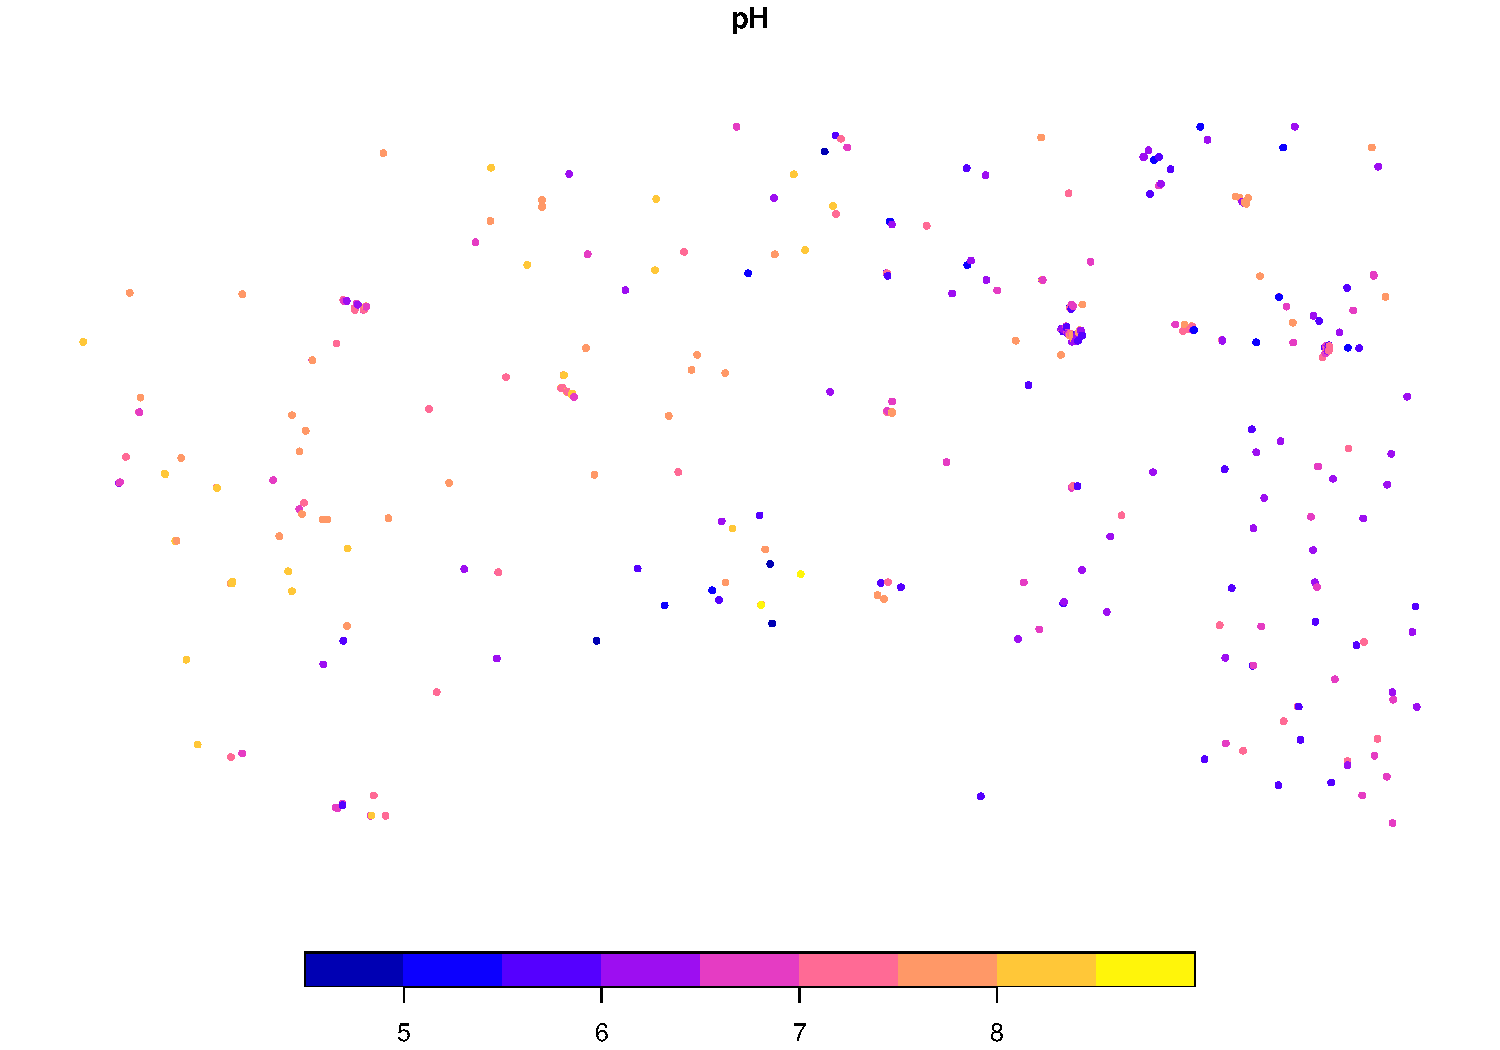
\includegraphics[keepaspectratio]{SoilFER-Integrated-soil-information-for-decision-making_files/figure-latex/shp-to-sf-hidden-1.pdf}}

\paragraph*{Setting and Reprojecting CRS for vector data}\label{setting-and-reprojecting-crs-for-vector-data}
\addcontentsline{toc}{paragraph}{Setting and Reprojecting CRS for vector data}

It is good practice to always confirm the Coordinate Reference System (CRS) of your spatial data. If the CRS is missing or incorrectly specified, spatial operations such as buffering, distance, and overlay may fail or return misleading results.

As shown previously, the CRS can be defined when creating an sf object (e.g., with \texttt{st\_as\_sf()}). You can inspect the CRS of an \texttt{sf} object with \texttt{st\_crs()}. If the CRS is missing, you can assign it with \texttt{st\_set\_crs()}. To reproject the data into a different CRS (i.e., change the coordinate values to a new reference system), use \texttt{st\_transform()}.

Example: Converting the sf object \texttt{soil\_sf} from Geographic WGS84 (EPSG:4326) to WGS 84 / Pseudo-Mercator (EPSG:3857), a projection commonly used for web mapping.

\begin{Shaded}
\begin{Highlighting}[]
\NormalTok{sf\_3857 }\OtherTok{\textless{}{-}} \FunctionTok{st\_transform}\NormalTok{(soil\_sf, }\DecValTok{3857}\NormalTok{)}

\CommentTok{\# Preview of the projected object}
\FunctionTok{head}\NormalTok{(sf\_3857)}
\end{Highlighting}
\end{Shaded}

\begin{verbatim}
## Simple feature collection with 6 features and 8 fields
## Geometry type: POINT
## Dimension:     XY
## Bounding box:  xmin: -11352220 ymin: 4645745 xmax: -11324070 ymax: 4761739
## Projected CRS: WGS 84 / Pseudo-Mercator
##     ProfID top bottom     Clay Silt Sand    SOC   pH
## 1 PROF0003   0     30 20.46297 55.9 23.6 1.5744 8.13
## 2 PROF0004   0     30 22.83169 57.9 19.3 1.3520 6.12
## 3 PROF0005   0     30 26.41016 58.4 15.2 1.5100 7.25
## 4 PROF0006   0     30 19.79542 54.9 25.3 1.6500 6.75
## 5 PROF0007   0     30 25.51856 54.2 20.3 1.6972 7.21
## 6 PROF0008   0     30 32.35233 57.7  9.9 1.4412 7.84
##                    geometry
## 1 POINT (-11352221 4731687)
## 2 POINT (-11330456 4645745)
## 3 POINT (-11330245 4646078)
## 4 POINT (-11329955 4646172)
## 5 POINT (-11326387 4661659)
## 6 POINT (-11324071 4761739)
\end{verbatim}

\paragraph*{\texorpdfstring{Inspecting and manipulating \texttt{\{sf\}} Object}{Inspecting and manipulating \{sf\} Object}}\label{inspecting-and-manipulating-sf-object}
\addcontentsline{toc}{paragraph}{Inspecting and manipulating \texttt{\{sf\}} Object}

Because \texttt{sf} objects inherit from the \texttt{data.frame} class, you can explore an sf object with the same tools as data frames (\texttt{class()},\texttt{str()}, \texttt{summary()}), plus a few \texttt{\{sf\}} helpers (\texttt{st\_geometry\_type()}).

\begin{Shaded}
\begin{Highlighting}[]
\CommentTok{\# Check structure}
\FunctionTok{str}\NormalTok{(soil\_sf)}
\end{Highlighting}
\end{Shaded}

\begin{verbatim}
## Classes 'sf' and 'data.frame':   411 obs. of  9 variables:
##  $ ProfID  : chr  "PROF0003" "PROF0004" "PROF0005" "PROF0006" ...
##  $ top     : int  0 0 0 0 0 0 0 0 0 0 ...
##  $ bottom  : int  30 30 30 30 30 30 30 30 30 30 ...
##  $ Clay    : num  20.5 22.8 26.4 19.8 25.5 ...
##  $ Silt    : num  55.9 57.9 58.4 54.9 54.2 57.7 57.5 63 56.5 59.2 ...
##  $ Sand    : num  23.6 19.3 15.2 25.3 20.3 9.9 8.7 10.5 9.3 5.8 ...
##  $ SOC     : num  1.57 1.35 1.51 1.65 1.7 ...
##  $ pH      : num  8.13 6.12 7.25 6.75 7.21 7.84 7.23 6.2 6.6 7.72 ...
##  $ geometry:sfc_POINT of length 411; first list element:  'XY' num  -102 39.1
##  - attr(*, "sf_column")= chr "geometry"
##  - attr(*, "agr")= Factor w/ 3 levels "constant","aggregate",..: NA NA NA NA NA NA NA NA
##   ..- attr(*, "names")= chr [1:8] "ProfID" "top" "bottom" "Clay" ...
\end{verbatim}

\begin{Shaded}
\begin{Highlighting}[]
\CommentTok{\# Summary of attributes + geometry}
\FunctionTok{summary}\NormalTok{(soil\_sf)}
\end{Highlighting}
\end{Shaded}

\begin{verbatim}
##     ProfID               top        bottom        Clay       
##  Length:411         Min.   :0   Min.   :30   Min.   : 2.912  
##  Class :character   1st Qu.:0   1st Qu.:30   1st Qu.:23.081  
##  Mode  :character   Median :0   Median :30   Median :29.824  
##                     Mean   :0   Mean   :30   Mean   :30.146  
##                     3rd Qu.:0   3rd Qu.:30   3rd Qu.:37.148  
##                     Max.   :0   Max.   :30   Max.   :65.460  
##       Silt            Sand            SOC              pH       
##  Min.   : 3.60   Min.   : 0.30   Min.   :0.120   Min.   :4.500  
##  1st Qu.:48.85   1st Qu.: 5.00   1st Qu.:1.104   1st Qu.:6.195  
##  Median :55.80   Median : 9.80   Median :1.600   Median :6.905  
##  Mean   :53.24   Mean   :16.59   Mean   :1.801   Mean   :6.881  
##  3rd Qu.:61.80   3rd Qu.:19.30   3rd Qu.:2.268   3rd Qu.:7.660  
##  Max.   :81.40   Max.   :92.50   Max.   :7.317   Max.   :8.830  
##           geometry  
##  POINT        :411  
##  epsg:4326    :  0  
##  +proj=long...:  0  
##                     
##                     
## 
\end{verbatim}

\begin{Shaded}
\begin{Highlighting}[]
\CommentTok{\# Check the geometry type. Use head to avoid long printing}
\FunctionTok{head}\NormalTok{(}\FunctionTok{st\_geometry\_type}\NormalTok{(soil\_sf))}
\end{Highlighting}
\end{Shaded}

\begin{verbatim}
## [1] POINT POINT POINT POINT POINT POINT
## 18 Levels: GEOMETRY POINT LINESTRING POLYGON MULTIPOINT ... TRIANGLE
\end{verbatim}

\begin{Shaded}
\begin{Highlighting}[]
\CommentTok{\# Check the CRS:}
\FunctionTok{st\_crs}\NormalTok{(soil\_sf)}
\end{Highlighting}
\end{Shaded}

\begin{verbatim}
## Coordinate Reference System:
##   User input: WGS 84 
##   wkt:
## GEOGCRS["WGS 84",
##     DATUM["World Geodetic System 1984",
##         ELLIPSOID["WGS 84",6378137,298.257223563,
##             LENGTHUNIT["metre",1]]],
##     PRIMEM["Greenwich",0,
##         ANGLEUNIT["degree",0.0174532925199433]],
##     CS[ellipsoidal,2],
##         AXIS["latitude",north,
##             ORDER[1],
##             ANGLEUNIT["degree",0.0174532925199433]],
##         AXIS["longitude",east,
##             ORDER[2],
##             ANGLEUNIT["degree",0.0174532925199433]],
##     ID["EPSG",4326]]
\end{verbatim}

\begin{Shaded}
\begin{Highlighting}[]
\CommentTok{\# Check the spatial extent of the object:}
\FunctionTok{st\_bbox}\NormalTok{(soil\_sf)}
\end{Highlighting}
\end{Shaded}

\begin{verbatim}
##       xmin       ymin       xmax       ymax 
## -101.97873   37.01713  -94.70964   39.98839
\end{verbatim}

\texttt{\{sf\}} objects can be manipulated in the same way as standard data frames while retaining all spatial information.
Base R and \texttt{\{dplyr\}} verbs such as \texttt{filter()}, \texttt{select()}, \texttt{mutate()}, can be directly applied on \texttt{sf} objects .

\begin{Shaded}
\begin{Highlighting}[]
\CommentTok{\# Subset sf rows and columns using the pipping (\%\textgreater{}\%) operator with \{dplyr\}}
\NormalTok{alkaline }\OtherTok{\textless{}{-}}\NormalTok{ soil\_sf }\SpecialCharTok{\%\textgreater{}\%}
  \FunctionTok{filter}\NormalTok{(pH }\SpecialCharTok{\textgreater{}} \FloatTok{7.4}\NormalTok{) }\SpecialCharTok{\%\textgreater{}\%}
  \FunctionTok{select}\NormalTok{(ProfID, pH) }\SpecialCharTok{\%\textgreater{}\%}
  \FunctionTok{mutate}\NormalTok{(}\AttributeTok{alkaline =} \ConstantTok{TRUE}\NormalTok{)}
\CommentTok{\# Preview alkaline data}
\FunctionTok{head}\NormalTok{(alkaline)}
\end{Highlighting}
\end{Shaded}

\begin{verbatim}
## Simple feature collection with 6 features and 3 fields
## Geometry type: POINT
## Dimension:     XY
## Bounding box:  xmin: -101.9787 ymin: 38.50486 xmax: -101.5333 ymax: 39.27917
## Geodetic CRS:  WGS 84
##     ProfID   pH                   geometry alkaline
## 1 PROF0003 8.13 POINT (-101.9787 39.06988)     TRUE
## 2 PROF0008 7.84 POINT (-101.7259 39.27917)     TRUE
## 3 PROF0012 7.72  POINT (-101.667 38.83208)     TRUE
## 4 PROF0013 8.29  POINT (-101.536 38.50828)     TRUE
## 5 PROF0014 8.28  POINT (-101.534 38.50785)     TRUE
## 6 PROF0015 8.29 POINT (-101.5333 38.50486)     TRUE
\end{verbatim}

\paragraph*{Geometry Operations}\label{geometry-operations}
\addcontentsline{toc}{paragraph}{Geometry Operations}

Geometry operations help you \textbf{create new geometries} (e.g., buffers) and \textbf{combine layers} (e.g., clip points to a boundary). In soil science, they are often used to define sampling influence areas, restrict data to an administrative unit, or summarize results by region.

For distance and area-based operations (buffers, distances, areas), work in a Projected CRS (units in metres), not in lon/lat degrees.
Before any geometry operation, make sure both layers are in the same CRS.

\subparagraph*{Buffering Plots (Influence Area)}\label{buffering-plots-influence-area}
\addcontentsline{toc}{subparagraph}{Buffering Plots (Influence Area)}

Buffers are regions created at a fixed distance around geometries (points, lines, or polygons).\\
In soil applications, buffers can represent:

\begin{itemize}
\tightlist
\item
  The influence area of a contaminating facility (polygon geometry).
\item
  Proximity zones around rivers or roads (line geometry).
\item
  Buffer zones around soil sampling points to define their spatial influence (point geometry).
\end{itemize}

The function \texttt{st\_buffer()} is used for this. If the input dataset is in a Geographic Coordinate System (longitude/latitude in degrees), you should first transform it to a Projected Coordinate System (units in metres) before buffering.

\begin{Shaded}
\begin{Highlighting}[]
\CommentTok{\# Original KSSL data is in WGS84 EPSG:4326  geographic coordinates(lon/lat)}
\CommentTok{\# Transform the subset of alkaline soils to NAD83 / UTM 14N (EPSG: 26914)}
\NormalTok{alkaline\_utm }\OtherTok{\textless{}{-}} \FunctionTok{st\_transform}\NormalTok{(alkaline, }\AttributeTok{crs =} \DecValTok{26914}\NormalTok{)  }\CommentTok{\# UTM 14N, distance in metres}

\CommentTok{\# Create a 1 km buffer around each plot}
\NormalTok{plots\_buffer\_1k }\OtherTok{\textless{}{-}} \FunctionTok{st\_buffer}\NormalTok{(alkaline\_utm, }\AttributeTok{dist =} \DecValTok{1000}\NormalTok{)}

\CommentTok{\# Plot buffers (first 3 plots) and then overlay the same points}
\FunctionTok{plot}\NormalTok{(}\FunctionTok{st\_geometry}\NormalTok{(plots\_buffer\_1k[}\DecValTok{1}\SpecialCharTok{:}\DecValTok{3}\NormalTok{, ]), }
     \AttributeTok{col =} \FunctionTok{rgb}\NormalTok{(}\DecValTok{0}\NormalTok{, }\DecValTok{0}\NormalTok{, }\DecValTok{1}\NormalTok{, }\FloatTok{0.3}\NormalTok{), }\AttributeTok{border =} \StringTok{"blue"}\NormalTok{,}
     \AttributeTok{main =} \StringTok{"Plot of first 3 alkaline soils with 1 km buffers"}\NormalTok{)}
\CommentTok{\# Overlay the original sample locations}
\FunctionTok{plot}\NormalTok{(}\FunctionTok{st\_geometry}\NormalTok{(alkaline\_utm[}\DecValTok{1}\SpecialCharTok{:}\DecValTok{3}\NormalTok{, ]), }
     \AttributeTok{add =} \ConstantTok{TRUE}\NormalTok{, }\AttributeTok{pch =} \DecValTok{16}\NormalTok{, }\AttributeTok{col =} \StringTok{"red"}\NormalTok{)}
\end{Highlighting}
\end{Shaded}

\begin{figure}

{\centering \includegraphics[width=0.7\linewidth]{SoilFER-Training-Resources/01_outputs/buffer_samples} 

}

\caption{1 km buffer around sampling points }\label{fig:unnamed-chunk-2}
\end{figure}

\subparagraph*{Clip Soil Data to Defined Boundaries}\label{clip-soil-data-to-defined-boundaries}
\addcontentsline{toc}{subparagraph}{Clip Soil Data to Defined Boundaries}

In soil data management workflows, it is common to restrict analyses to a defined study area (e.g., a county, district, watershed, or project boundary). This helps ensure that summaries, maps, and models are computed only for the relevant spatial extent.

Two core operations are used repeatedly in Soil Data Management and Digital Soil Mapping:

\begin{itemize}
\item
  \textbf{Clip / subset by boundary} (\texttt{st\_intersection()}): keeps only the features (or parts of features) that fall inside a target boundary.
\item
  \textbf{Dissolve boundaries} (\texttt{st\_union()}): merges multiple polygons into a single boundary by removing internal borders.
\end{itemize}

Use \textbf{clipping} to restrict soil profiles, samples, or observations to a target area before analysis or reporting.

Use \textbf{dissolving} to build a clean study boundary for masking, cropping, mapping, or aggregating results at a higher level.

\textbf{Example 1: Clip sampling points to one administrative unit}

In this example, we clip KSSL sampling points to Riley County. The steps are:

\begin{itemize}
\item
  Read the administrative boundaries layer.
\item
  Transform it to the CRS of the soil points (so layers align).
\item
  Select the target polygon (Riley).
\item
  Clip the soil points to that polygon.
\end{itemize}

\begin{Shaded}
\begin{Highlighting}[]
\CommentTok{\# Read administrative boundaries (example file)}
\NormalTok{admin }\OtherTok{\textless{}{-}} \FunctionTok{st\_read}\NormalTok{(}\StringTok{"01\_data/module1/shapes/Tiger\_2020\_Counties.shp"}\NormalTok{)}
\CommentTok{\# Ensure both layers share the same CRS}
\NormalTok{admin }\OtherTok{\textless{}{-}} \FunctionTok{st\_transform}\NormalTok{(admin, }\FunctionTok{st\_crs}\NormalTok{(soil\_sf))}
\CommentTok{\# Example: select one unit (replace with your column/value)}
\NormalTok{study\_area }\OtherTok{\textless{}{-}}\NormalTok{ admin[admin}\SpecialCharTok{$}\NormalTok{NAME }\SpecialCharTok{==} \StringTok{"Riley"}\NormalTok{, ]}
\CommentTok{\# Keep only points inside the study area}
\NormalTok{soil\_clip }\OtherTok{\textless{}{-}} \FunctionTok{st\_intersection}\NormalTok{(soil\_sf, study\_area)}
\CommentTok{\# Plot result}
\FunctionTok{plot}\NormalTok{(}\FunctionTok{st\_geometry}\NormalTok{(study\_area), }\AttributeTok{col =} \ConstantTok{NA}\NormalTok{, }\AttributeTok{border =} \StringTok{"black"}\NormalTok{, }\AttributeTok{main=}\StringTok{"Sampled soils in Riley County"}\NormalTok{, }\AttributeTok{cex.main =} \DecValTok{1}\NormalTok{ )}
\FunctionTok{plot}\NormalTok{(}\FunctionTok{st\_geometry}\NormalTok{(soil\_clip), }\AttributeTok{add =} \ConstantTok{TRUE}\NormalTok{, }\AttributeTok{pch =} \DecValTok{16}\NormalTok{, }\AttributeTok{col =} \StringTok{"red"}\NormalTok{, }\AttributeTok{cex =} \FloatTok{0.6}\NormalTok{)}
\end{Highlighting}
\end{Shaded}

\begin{figure}

{\centering \includegraphics[width=0.5\linewidth]{SoilFER-Training-Resources/01_outputs/riley_samples} 

}

\caption{Sampled soils in Riley County}\label{fig:unnamed-chunk-3}
\end{figure}

In this case, \texttt{soil\_clip} preserves all attributes from the original sampling dataset (\texttt{soil\_sf}) and includes the attributes of the administrative polygon \texttt{admin} at each point.

\textbf{Example 2: Dissolve polygons to create a single study region boundary}

Dissolving is useful when you want a single boundary for a larger study region. For example, you may want to combine all counties into a single Kansas state outline (or merge multiple polygons representing a project area).

\texttt{st\_union()} merges all polygons into one geometry and removes internal borders.

\begin{Shaded}
\begin{Highlighting}[]
\CommentTok{\# Dissolve all counties into one Kansas boundary}
\NormalTok{admin\_dissolved }\OtherTok{\textless{}{-}} \FunctionTok{st\_union}\NormalTok{(admin)}
\CommentTok{\# Plot comparison: before vs after dissolve}
\CommentTok{\# Adjust graphics settings to 1 row x 2 columns layout with tight margins}
\NormalTok{op }\OtherTok{\textless{}{-}} \FunctionTok{par}\NormalTok{(}
  \AttributeTok{mfrow =} \FunctionTok{c}\NormalTok{(}\DecValTok{1}\NormalTok{, }\DecValTok{2}\NormalTok{),}
  \AttributeTok{mar =} \FunctionTok{c}\NormalTok{(}\FloatTok{0.5}\NormalTok{, }\FloatTok{0.5}\NormalTok{, }\FloatTok{0.1}\NormalTok{, }\FloatTok{0.5}\NormalTok{),  }\CommentTok{\# very small top margin}
  \AttributeTok{xaxs =} \StringTok{"i"}\NormalTok{, }\AttributeTok{yaxs =} \StringTok{"i"}
\NormalTok{)}
\FunctionTok{plot}\NormalTok{(}\FunctionTok{st\_geometry}\NormalTok{(admin[}\DecValTok{1}\NormalTok{]),}
     \AttributeTok{col =} \ConstantTok{NA}\NormalTok{, }\AttributeTok{border =} \StringTok{"black"}\NormalTok{,}
     \AttributeTok{axes =} \ConstantTok{FALSE}\NormalTok{, }\AttributeTok{asp =} \DecValTok{1}\NormalTok{)}
\FunctionTok{title}\NormalTok{(}\StringTok{"Before dissolve"}\NormalTok{, }\AttributeTok{line =} \SpecialCharTok{{-}}\FloatTok{0.6}\NormalTok{, }\AttributeTok{cex.main =} \FloatTok{0.95}\NormalTok{)}
\FunctionTok{plot}\NormalTok{(}\FunctionTok{st\_geometry}\NormalTok{(admin\_dissolved),}
     \AttributeTok{col =} \ConstantTok{NA}\NormalTok{, }\AttributeTok{border =} \StringTok{"black"}\NormalTok{,}
     \AttributeTok{axes =} \ConstantTok{FALSE}\NormalTok{, }\AttributeTok{asp =} \DecValTok{1}\NormalTok{)}
\FunctionTok{title}\NormalTok{(}\StringTok{"After dissolve"}\NormalTok{, }\AttributeTok{line =} \SpecialCharTok{{-}}\FloatTok{0.6}\NormalTok{, }\AttributeTok{cex.main =} \FloatTok{0.95}\NormalTok{)}
\CommentTok{\# restore graphics settings}
\FunctionTok{par}\NormalTok{(op)}
\end{Highlighting}
\end{Shaded}

\begin{figure}
\includegraphics[width=1\linewidth]{SoilFER-Training-Resources/01_outputs/dissolve_before_after} \caption{Dissolving polygons on Kansas County vector data}\label{fig:unnamed-chunk-4}
\end{figure}

\subparagraph*{Spatial Relationships and Joins}\label{spatial-relationships-and-joins}
\addcontentsline{toc}{subparagraph}{Spatial Relationships and Joins}

Spatial relationships help answer questions about how spatial features relate to one another (e.g., whether a point falls inside a polygon, or how far two features are apart).

\textbf{Spatial predicates} (return TRUE/FALSE relationships):

\begin{itemize}
\item
  \texttt{st\_intersects()} (touch/overlap)
\item
  \texttt{st\_within()} (inside)
\item
  \texttt{st\_distance()} (distance between features)
\end{itemize}

\textbf{Spatial joins} attach attributes from one layer to another:

\begin{itemize}
\tightlist
\item
  \texttt{st\_join()} (e.g., assign each soil profile to an administrative unit)
\end{itemize}

Example: assign each sampling point to an administrative polygon.

\begin{Shaded}
\begin{Highlighting}[]
\CommentTok{\# Ensure both layers share the same CRS}
\NormalTok{alkaline }\OtherTok{\textless{}{-}} \FunctionTok{st\_transform}\NormalTok{(alkaline, }\FunctionTok{st\_crs}\NormalTok{(admin))}
\CommentTok{\# Join admin attributes to points (points inherit polygon attributes)}
\NormalTok{alkaline\_with\_admin }\OtherTok{\textless{}{-}} \FunctionTok{st\_join}\NormalTok{(alkaline, admin, }\AttributeTok{join =}\NormalTok{ st\_within)}
\CommentTok{\# Preview result}
\FunctionTok{head}\NormalTok{(alkaline\_with\_admin)}
\end{Highlighting}
\end{Shaded}

\begin{verbatim}
## Simple feature collection with 6 features and 20 fields
## Geometry type: POINT
## Dimension:     XY
## Bounding box:  xmin: -101.9787 ymin: 38.50486 xmax: -101.5333 ymax: 39.27917
## Geodetic CRS:  WGS 84
##     ProfID   pH alkaline STATEFP COUNTYFP COUNTYNS GEOID    NAME
## 1 PROF0003 8.13     TRUE      20      199 00485060 20199 Wallace
## 2 PROF0008 7.84     TRUE      20      181 00485053 20181 Sherman
## 3 PROF0012 7.72     TRUE      20      199 00485060 20199 Wallace
## 4 PROF0013 8.29     TRUE      20      203 00485062 20203 Wichita
## 5 PROF0014 8.28     TRUE      20      203 00485062 20203 Wichita
## 6 PROF0015 8.29     TRUE      20      203 00485062 20203 Wichita
##         NAMELSAD LSAD CLASSFP MTFCC CSAFP CBSAFP METDIVFP FUNCSTAT AWATER
## 1 Wallace County   06      H1 G4020  <NA>   <NA>     <NA>        A 140936
## 2 Sherman County   06      H1 G4020  <NA>   <NA>     <NA>        A 548248
## 3 Wallace County   06      H1 G4020  <NA>   <NA>     <NA>        A 140936
## 4 Wichita County   06      H1 G4020  <NA>   <NA>     <NA>        A  61987
## 5 Wichita County   06      H1 G4020  <NA>   <NA>     <NA>        A  61987
## 6 Wichita County   06      H1 G4020  <NA>   <NA>     <NA>        A  61987
##      INTPTLAT     INTPTLON                             GlobalID
## 1 +38.9266259 -101.7711031 5d2c40a3-7c2d-4f48-879b-11e53b1bc366
## 2 +39.3513521 -101.7198590 111d187f-9907-4a48-8678-a1bed6840eb9
## 3 +38.9266259 -101.7711031 5d2c40a3-7c2d-4f48-879b-11e53b1bc366
## 4 +38.4819222 -101.3474341 c1ad0367-fe83-4ee2-91fb-256e33e36857
## 5 +38.4819222 -101.3474341 c1ad0367-fe83-4ee2-91fb-256e33e36857
## 6 +38.4819222 -101.3474341 c1ad0367-fe83-4ee2-91fb-256e33e36857
##                     geometry
## 1 POINT (-101.9787 39.06988)
## 2 POINT (-101.7259 39.27917)
## 3  POINT (-101.667 38.83208)
## 4  POINT (-101.536 38.50828)
## 5  POINT (-101.534 38.50785)
## 6 POINT (-101.5333 38.50486)
\end{verbatim}

\paragraph*{\texorpdfstring{Visualizing \texttt{\{sf\}} Objects}{Visualizing \{sf\} Objects}}\label{visualizing-sf-objects}
\addcontentsline{toc}{paragraph}{Visualizing \texttt{\{sf\}} Objects}

As shown previously, \texttt{\{sf\}} objects can be quickly visualized using the base R \texttt{plot()} function. This is convenient for fast checks (e.g., verifying geometry and extent), but it offers limited control over plot appearance and legend design.

In contrast, \texttt{\{ggplot2\}} provides a consistent \emph{`grammar of graphics'} that makes it easier to produce publication-ready maps. Key benefits include:

\begin{itemize}
\item
  Full control of aesthetics (colors, symbol size, line width, transparency) and clear legends.
\item
  High-quality themes and consistent styling across figures (useful in reports and publications).
\item
  Easy layering of multiple spatial objects (points, polygons, buffers, rasters---when combined with other tools).
\item
  Faceting to compare maps by groups (e.g., land use class, sampling campaign, depth interval).
\end{itemize}

In \texttt{\{ggplot2\}}, spatial geometries are plotted with \texttt{geom\_sf().}

\begin{Shaded}
\begin{Highlighting}[]
\FunctionTok{library}\NormalTok{(ggplot2)}
\FunctionTok{ggplot}\NormalTok{(}\AttributeTok{data =}\NormalTok{ soil\_sf) }\SpecialCharTok{+}
  \FunctionTok{geom\_sf}\NormalTok{(}\FunctionTok{aes}\NormalTok{(}\AttributeTok{color =}\NormalTok{ pH), }\AttributeTok{size =} \DecValTok{2}\NormalTok{) }\SpecialCharTok{+}
  \FunctionTok{scale\_color\_viridis\_c}\NormalTok{() }\SpecialCharTok{+}
  \FunctionTok{theme\_minimal}\NormalTok{() }\SpecialCharTok{+}
  \FunctionTok{labs}\NormalTok{(}
    \AttributeTok{title =} \StringTok{"Soil sampling sites – pH"}\NormalTok{,}
    \AttributeTok{color =} \StringTok{"pH"}
\NormalTok{  )}
\end{Highlighting}
\end{Shaded}

\begin{figure}
\includegraphics[width=1\linewidth]{SoilFER-Training-Resources/01_outputs/ggplot_ph} \caption{Visualization of pH values with ggplot2}\label{fig:unnamed-chunk-5}
\end{figure}

The possibilities for visualization with \texttt{\{ggplot2\}} are extensive. For more examples and options, see the \texttt{\{ggplot2\}} documentation and the \texttt{\{sf\}} vignettes on plotting with \texttt{geom\_sf()}.

\begin{center}\rule{0.5\linewidth}{0.5pt}\end{center}

\subsection{Preparing Raster Covariates}\label{preparing-raster-covariates}

The workflows presented in this tutorial use environmental covariates as proxies to describe the spatial variation of soil properties. These covariates support two key steps:

\begin{itemize}
\item
  \textbf{Sampling design}: covariates are used to identify environmental clusters that should be sampled, helping maximize the representation of soil variability while optimizing sampling effort.
\item
  \textbf{Digital Soil Mapping}: soil properties measured at known point locations (vector data) are related to environmental characteristics (raster covariates) to train statistical or machine learning models that predict soil properties continuously across space.
\end{itemize}

The preparation of covariates is a time-consuming task. Therefore this tutorial uses a pre-compiled set of environmental covariates to fulfil these tasks. It assembles five categories of environmental covariates cloud-optimized GeoTIFF files.

\textbf{Climate data} is sourced from two complementary products.

\begin{itemize}
\item
  \textbf{CHELSA} (Climatologies at High resolution for the Earth's Land Surface Areas) provides long-term bioclimatic variables including mean annual temperature (bio1), annual precipitation (bio12), and extreme temperature and precipitation metrics (bio5, bio6, bio13, bio14, bio16, bio17), alongside potential evapotranspiration computed using the Penman-Monteith method and surface wind statistics.
\item
  \textbf{TerraClimate} contributes monthly time series of maximum and minimum temperature, precipitation, and potential evapotranspiration spanning 1981 to the present, which are exported as multi-band images for subsequent temporal aggregation in R.
\end{itemize}

\textbf{Terrain data} is derived from the USGS SRTM 30 m Digital Elevation Model, from which slope, aspect, Topographic Position Index (TPI), and hillshade are computed on-the-fly within GEE. Geomorphological landform classification at 90 m resolution is obtained from the \texttt{Geomorpho90m} dataset. Additionally, pre-computed terrain derivatives at 250 m resolution (elevation, slope, curvature, TPI, TWI) are loaded from the FAO GSP shared GEE asset library hosted at \texttt{projects/digital-soil-mapping-gsp-fao}.

\textbf{Vegetation and soil indices} are computed from Sentinel-2 Surface Reflectance imagery (Copernicus/S2\_SR\_HARMONIZED), filtered to scenes with less than 10\% cloud cover and cloud-masked using the QA60 quality band. The script computes the Normalized Difference Vegetation Index (NDVI), Enhanced Vegetation Index (EVI), Normalized Difference Bareness and Soil Index (NDBSI), Redness Index, Brightness Index, NBR+, and the Visible-Near-Short-wave Infrared Index (VNSIR). Seasonal vegetation dynamics are additionally captured through MODIS FPAR mean and standard deviation layers for four three-month periods covering the full annual cycle.

\textbf{Soil Available Water Content} represent the mean available water capacity (AWC - in mm) of soil from 0 to 200 cm depth.

\textbf{Land cover} is represented by the ESA WorldCover 2021 product at 10 m resolution, from which a cropland mask is derived by isolating the cropland class (value 40) for use in masking or stratified analyses.

\begin{quote}
Note: users need to have a google account to access the covariate data.
\end{quote}

\paragraph*{Download Covariate Rasters}\label{download-covariate-rasters}
\addcontentsline{toc}{paragraph}{Download Covariate Rasters}

A dedicate Google Drive folder has been created to store large raster files used in this tutorial. Users can obtain the data directly from the folder \texttt{rasters} following link:
\url{https://drive.google.com/drive/folders/1K7tq9zX5HsqbqWcNoT27WtfPtehcKBCu}

Data in this folder includes:

\begin{itemize}
\tightlist
\item
  \href{https://drive.google.com/file/d/1wh6xSW03YKrCHScJJa0c_cSA1XZ8tYY-/view?usp=drive_link}{\textbf{Cropland\_Mask\_KANSAS.tif}} (22.5 mb): Binary raster with presence (1) and absence (NA) of crops in Kansas at 20 meter resolution. This file is used as a mask to avoid non-cropped areas in the analyses.
\item
  \href{https://drive.google.com/file/d/1wURPmPLi2LdYq6zBhZN1e91EiiZsk8oX/view?usp=drive_link}{\textbf{Environmental\_Covariates\_250m\_KANSAS.tif}} (203.2 mb): Multi-layer raster stack with climatic, remote sensing, topographic information at 250 meter resolution.
\item
  \href{https://drive.google.com/file/d/1xf89gn4pBKsb5ynVIfKZd4MbT3ZL1Nf2/view?usp=drive_link}{\textbf{HighRes\_Covariates\_100m\_Kansas.tif}} (535.6 mb). 100 m resolution rasters with remote sensing derived information.
\item
  \href{https://drive.google.com/file/d/14KmmjjTfVD7jTEuQqCLkfcQmXy0VBDkA/view?usp=drive_link}{\textbf{DEM\_KANSAS.tif}} (21.4 mb). 100 m resolution rasters with remote sensing derived information.
\item
  \href{https://drive.google.com/file/d/1rESziVFlEvEEmrKacb88R1pKZxbrU7qS/view?usp=drive_link}{\textbf{Slope\_KANSAS.tif}} (61.2 mb). 100 m resolution rasters with remote sensing derived information.
\item
  {[}\textbf{Geomorphon\_Landforms\_KANSAS}{]}(\citeproc{ref-amatulli2020_geomorpho90m}{Amatulli \emph{et al.}, 2020})(\url{https://drive.google.com/file/d/1E03U42UPl9SKMfUGZZ8qDCno2H_kPxUB/view?usp=drive_link}) (14.9 mb). 90 m resolution raster of geomorphological types from Geomorpho90m -- Global High-Resolution Geomorphometry Layers.
\item
  \href{https://drive.google.com/file/d/1TyyErHkQeNW9Q_wchW9Fa_0UpdaWS_-_/view?usp=drive_link}{\textbf{TerraClimate\_AvgTemp\_1981\_2023\_KANSAS.tif}} (17.7 mb). 100 m TerraClimate monthly averaged Temperature rasters from 1981-2023.
\item
  \href{https://drive.google.com/file/d/1b9wM3zwggBFS98pFEyWUFtpKN9ORq9we/view?usp=drive_link}{\textbf{TerraClimate\_PET\_1981\_2023\_KANSAS.tif}} (17.2 mb). 100 m TerraClimate monthly averaged Potential Evapotranspiration rasters from 1981-2023.
\item
  \href{https://drive.google.com/file/d/1xq6y8jNUjDbipXHQE1w67f_vxQeXACkH/view?usp=drive_link}{\textbf{TerraClimate\_Precip\_1981\_2023\_KANSAS.tif}} (11.9 mb). 100 m TerraClimate monthly accumulated mean Precipitation rasters from 1981-2023.
\item
  {[}\textbf{sol\_available.water.capacity\_usda.mm\_m\_250m\_0..200cm\_1950..2017\_v0.1.tif}{]}(\citeproc{ref-gupta_zenodo_2019}{Gupta and Hengl, 2019})(\url{https://drive.google.com/file/d/1nG0yCr-tNPzeeEvzcGrtdQxRHnQ6NMH5/view?usp=drive_link}). 250-meter resolution geospatial raster dataset representing the mean available water capacity (AWC - in mm) of soil from 0 to 200 cm depth.
\item
  {[}\textbf{ESA\_WorldCover\_2021\_KANSAS}{]}(\citeproc{ref-zanaga2022_worldcover2021_v200}{Zanaga \emph{et al.}, 2022})(\url{https://drive.google.com/file/d/1xq6y8jNUjDbipXHQE1w67f_vxQeXACkH/view?usp=drive_link}) (11.9 mb). 10 m resolution rasters of landcover types from the European Space Agency WorldCover, based on Sentinel-1 and Sentinel-2 data.
\end{itemize}

\emph{Table. ESA WorldCover (global land cover) legend, the class codes and color in the Map band.}

\begin{longtable}[]{@{}rll@{}}
\toprule\noalign{}
Value & Class & Color (hex) \\
\midrule\noalign{}
\endhead
\bottomrule\noalign{}
\endlastfoot
10 & Tree cover & \texttt{\#006400} \\
20 & Shrubland & \texttt{\#ffbb22} \\
30 & Grassland & \texttt{\#ffff4c} \\
40 & Cropland & \texttt{\#f096ff} \\
50 & Built-up & \texttt{\#fa0000} \\
60 & Bare / sparse vegetation & \texttt{\#b4b4b4} \\
70 & Snow and ice & \texttt{\#f0f0f0} \\
80 & Permanent water bodies & \texttt{\#0064c8} \\
90 & Herbaceous wetland & \texttt{\#0096a0} \\
95 & Mangroves & \texttt{\#00cf75} \\
100 & Moss and lichen & \texttt{\#fae6a0} \\
\end{longtable}

\paragraph*{Obtain Covariate Data from Google Earth Engine (GEE)}\label{obtain-covariate-data-from-google-earth-engine-gee}
\addcontentsline{toc}{paragraph}{Obtain Covariate Data from Google Earth Engine (GEE)}

The data can also be generated directly using Google Earth Engine (GEE). GEE provides direct access to many environmental datasets through a unified interface, allowing analysts to extract, compute, and export ready-to-use covariate stacks for any region of interest using a single script.

The script provided with this training (\texttt{02\_scripts/module1/1\_gee\_soilfer\_env\_covariates.txt}) contains step-by-step instructions to download the covariate data from the GEE platform.

The data has been already processed for this training and is available to download from this \href{https://drive.google.com/drive/folders/1EGrkhbMTi2qglemuD_onegAqLWZb3BbT}{link}. Place these files into the \texttt{training\_data} folder within \texttt{01\_data/module1}and set the path for the covariate rasters and spectral data:

\begin{Shaded}
\begin{Highlighting}[]
\CommentTok{\# Define the relative path to the folder with the downloaded covariates}
\CommentTok{\# }\AlertTok{NOTE}\CommentTok{: Adapt this path to your project structure}
\NormalTok{  training\_dir }\OtherTok{\textless{}{-}}\StringTok{"01\_data/module1/training\_data"}
\end{Highlighting}
\end{Shaded}

\paragraph*{Running the GEE Script}\label{running-the-gee-script}
\addcontentsline{toc}{paragraph}{Running the GEE Script}

Copy the full contents of \texttt{1\_gee\_soilfer\_env\_covariates.txt} into the GEE Code Editor. Before running, review and adjust the configuration variables at the top of the script (Section 1) to match your study area and requirements.

The \texttt{aoi} variable defines the \texttt{area\ of\ interest}. For the training exercise, this is already configured to use the US Census TIGER state boundary layer:

\begin{Shaded}
\begin{Highlighting}[]
\KeywordTok{var}\NormalTok{ aoi }\OperatorTok{=}\NormalTok{ ee}\OperatorTok{.}\FunctionTok{FeatureCollection}\NormalTok{(}\StringTok{\textquotesingle{}TIGER/2018/States\textquotesingle{}}\NormalTok{)}
  \OperatorTok{.}\FunctionTok{filter}\NormalTok{(ee}\OperatorTok{.}\AttributeTok{Filter}\OperatorTok{.}\FunctionTok{eq}\NormalTok{(}\StringTok{\textquotesingle{}NAME\textquotesingle{}}\OperatorTok{,} \StringTok{\textquotesingle{}Kansas\textquotesingle{}}\NormalTok{))}\OperatorTok{;}
\end{Highlighting}
\end{Shaded}

To adapt the script to a different study area, replace this definition with a custom geometry or a different administrative boundary. Update \texttt{countryName} to a short descriptor used in the exported file names.

The date range for TerraClimate is controlled by \texttt{climateStartDate} and \texttt{climateEndDate}. The default configuration covers the full 1981--2023 record. For exploratory or training purposes, restricting this range (e.g., 2000--2023) reduces processing time and export file sizes.

Export spatial resolutions are defined individually for each product category, reflecting the native resolution of each data source: 250 m for the primary CHELSA/MODIS covariate stack, 100 m for high-resolution terrain and Sentinel-2 layers, 90 m for geomorphons, 20 m for the cropland mask, and 4000 m for TerraClimate time series.

Click \textbf{Run} to execute the script. Visualization layers (SRTM DEM, Sentinel-2 RGB composite, and cropland mask) will appear on the map immediately. Export tasks do not start automatically --- navigate to the \textbf{Tasks} tab in the right panel and click \textbf{Run} next to each pending task to initiate the exports to Google Drive.

\textbf{Processing Time and Quotas}

Large exports, particularly \textbf{TerraClimate} time series and \textbf{Sentinel-2} layers over large regions, can take tens of minutes to several hours depending on server load and area size. GEE free-tier accounts are subject to computation quotas. If a task fails with a computation timeout or memory error, consider reducing the export resolution or splitting the time series into shorter periods. Monitor task progress in the \textbf{Tasks} tab; completed files will appear in your \texttt{GEE\_Exports} Google Drive folder once finished.

Once all exports are complete, download the GeoTIFF files from Google Drive to your local working directory. In subsequent modules, these rasters will be loaded into R using the \texttt{terra} package and stacked into the covariate array used in the next modules.

\subsubsection{\texorpdfstring{Working with Raster Data using \texttt{\{terra\}}}{Working with Raster Data using \{terra\}}}\label{working-with-raster-data-using-terra}

The \texttt{\{terra\}} package is the main framework for working with raster spatial data in R. A raster represents space as a regular grid of cells, where each cell stores a value (e.g., elevation, land cover class, rainfall, SOC prediction). Raster layers are widely used in Digital Soil Mapping both as covariates (environmental predictors) and as model outputs (predicted soil properties).

In practice, a \texttt{terra::SpatRaster} object combines:

\begin{itemize}
\item
  Cell values: the data stored in the grid cells (continuous values like temperature, or categorical values like land cover).
\item
  Spatial geometry: the grid definition given by the extent (spatial coverage) and resolution (cell size).
\item
  CRS: the coordinate reference system used (e.g., WGS84, UTM).
\item
  Layers: a raster can have one layer (e.g., DEM, SOC) or multiple layers (a covariate stack).
\end{itemize}

\paragraph*{Importing and Exporting Raster Data}\label{importing-and-exporting-raster-data}
\addcontentsline{toc}{paragraph}{Importing and Exporting Raster Data}

Raster files are commonly distributed as GeoTIFFs (.tif). The function \texttt{rast()} reads both single-layer and multi-layer rasters. Rasters can be exported back to disk with \texttt{writeRaster()}.

\begin{Shaded}
\begin{Highlighting}[]
\FunctionTok{library}\NormalTok{(terra)}
\CommentTok{\# Read a single{-}layer raster (e.g., cropland mask or DEM)}
\NormalTok{crops }\OtherTok{\textless{}{-}} \FunctionTok{rast}\NormalTok{(}\FunctionTok{paste0}\NormalTok{(training\_dir,}\StringTok{"Cropland\_Mask\_KANSAS.tif"}\NormalTok{))}
\CommentTok{\# Read a multi{-}layer raster (e.g., environmental covariates stack)}
\NormalTok{covs }\OtherTok{\textless{}{-}} \FunctionTok{rast}\NormalTok{(}\FunctionTok{paste0}\NormalTok{(training\_dir,}\StringTok{"Environmental\_Covariates\_250m\_KANSAS.tif"}\NormalTok{))}
\end{Highlighting}
\end{Shaded}

To save raster data to disk use \texttt{writeRaster}:

\begin{Shaded}
\begin{Highlighting}[]
\CommentTok{\# Export a raster as GeoTIFF}
\FunctionTok{writeRaster}\NormalTok{(crops, }\StringTok{"03\_outputs/module1/Cropland\_Mask\_KANSAS.tif"}\NormalTok{, }\AttributeTok{overwrite =} \ConstantTok{TRUE}\NormalTok{) }\CommentTok{\# overwrites tif}
\end{Highlighting}
\end{Shaded}

\paragraph*{\texorpdfstring{Inspecting and Exploring \texttt{SpatRaster} Objects}{Inspecting and Exploring SpatRaster Objects}}\label{inspecting-and-exploring-spatraster-objects}
\addcontentsline{toc}{paragraph}{Inspecting and Exploring \texttt{SpatRaster} Objects}

Before analysis, inspect the spatial properties (extent, resolution, CRS), the number of layers, and the value ranges. This helps detect common issues such as mismatched CRS, unexpected resolution, incorrect extents, or missing data patterns.

\begin{Shaded}
\begin{Highlighting}[]
\CommentTok{\# Basic metadata (prints summary to console)}
\NormalTok{covs}
\CommentTok{\# Number of layers}
\FunctionTok{nlyr}\NormalTok{(covs)}
\CommentTok{\# Spatial properties}
\FunctionTok{ext}\NormalTok{(covs)}
\FunctionTok{res}\NormalTok{(covs)}
\FunctionTok{crs}\NormalTok{(covs)}
\CommentTok{\# Layer names (multi{-}layer rasters)}
\FunctionTok{names}\NormalTok{(covs)}
\CommentTok{\# Value ranges for the first 4 layers}
\FunctionTok{global}\NormalTok{(covs[[}\DecValTok{1}\SpecialCharTok{:}\DecValTok{4}\NormalTok{]], }\AttributeTok{fun =} \StringTok{"range"}\NormalTok{, }\AttributeTok{na.rm =} \ConstantTok{TRUE}\NormalTok{)}
\CommentTok{\# Histograms of the first 4 layers}
\CommentTok{\# Adjust graphics settings to 2 row x 2 columns layout with tight margins}
\NormalTok{op }\OtherTok{\textless{}{-}} \FunctionTok{par}\NormalTok{(}
  \AttributeTok{mfrow =} \FunctionTok{c}\NormalTok{(}\DecValTok{2}\NormalTok{, }\DecValTok{2}\NormalTok{),}
  \AttributeTok{mar  =} \FunctionTok{c}\NormalTok{(}\FloatTok{3.5}\NormalTok{, }\FloatTok{3.5}\NormalTok{, }\FloatTok{2.2}\NormalTok{, }\FloatTok{1.2}\NormalTok{),  }\CommentTok{\# more space around each panel}
  \AttributeTok{oma  =} \FunctionTok{c}\NormalTok{(}\DecValTok{1}\NormalTok{, }\DecValTok{1}\NormalTok{, }\DecValTok{1}\NormalTok{, }\DecValTok{1}\NormalTok{),          }\CommentTok{\# extra space around the whole figure}
  \AttributeTok{mgp  =} \FunctionTok{c}\NormalTok{(}\FloatTok{2.2}\NormalTok{, }\FloatTok{0.7}\NormalTok{, }\DecValTok{0}\NormalTok{)          }\CommentTok{\# axis title/labels spacing}
\NormalTok{)}

\ControlFlowTok{for}\NormalTok{ (i }\ControlFlowTok{in} \DecValTok{1}\SpecialCharTok{:}\DecValTok{4}\NormalTok{) \{}
  \FunctionTok{hist}\NormalTok{(covs[[i]],}
       \AttributeTok{main =} \FunctionTok{paste}\NormalTok{(}\StringTok{"Histogram of"}\NormalTok{, }\FunctionTok{names}\NormalTok{(covs)[i]),}
       \AttributeTok{xlab =} \FunctionTok{names}\NormalTok{(covs)[i])}
\NormalTok{\}}
\CommentTok{\# restore previous graphics settings}
\FunctionTok{par}\NormalTok{(op)}
\end{Highlighting}
\end{Shaded}

\begin{figure}
\includegraphics[width=1\linewidth]{SoilFER-Training-Resources/01_outputs/hist_covs} \caption{Visualization of histograms of covariates}\label{fig:unnamed-chunk-6}
\end{figure}

For most raster operations, rasters should share the same CRS, resolution, and extent. If they do not, they typically need adjustment using functions such as \texttt{project()}, \texttt{resample()}, and \texttt{crop()} before combining.

\paragraph*{Raster Visualization}\label{raster-visualization}
\addcontentsline{toc}{paragraph}{Raster Visualization}

Rasters can be quickly visualized using \texttt{plot()}. For multi-layer rasters, it is common to plot a subset of layers.

\begin{Shaded}
\begin{Highlighting}[]
\CommentTok{\# Plot single{-}layer crops raster mask}
\FunctionTok{plot}\NormalTok{(crops, }\AttributeTok{main=}\StringTok{"Cropland Mask"}\NormalTok{)}
\end{Highlighting}
\end{Shaded}

\begin{figure}
\includegraphics[width=1\linewidth]{SoilFER-Training-Resources/01_outputs/plot_crops} \caption{Visualization of raster crop mask}\label{fig:unnamed-chunk-7}
\end{figure}

\begin{Shaded}
\begin{Highlighting}[]
\CommentTok{\# Plot a multi{-}layer raster (e.g., environmental covariates stack)}
\FunctionTok{plot}\NormalTok{(covs)}
\end{Highlighting}
\end{Shaded}

\begin{figure}
\includegraphics[width=1\linewidth]{SoilFER-Training-Resources/01_outputs/plot_covs} \caption{Visualization of covariates}\label{fig:unnamed-chunk-8}
\end{figure}

You can also plot specific layers by name:

\begin{Shaded}
\begin{Highlighting}[]
\CommentTok{\# Plot Elevation and Temperature from the covs stack}
\CommentTok{\# Adjust graphics settings to 1 row x 2 columns layout with tight margins}
\NormalTok{op }\OtherTok{\textless{}{-}} \FunctionTok{par}\NormalTok{(}
  \AttributeTok{mfrow =} \FunctionTok{c}\NormalTok{(}\DecValTok{1}\NormalTok{, }\DecValTok{2}\NormalTok{),}
  \AttributeTok{mar =} \FunctionTok{c}\NormalTok{(}\FloatTok{0.5}\NormalTok{, }\FloatTok{0.5}\NormalTok{, }\FloatTok{0.5}\NormalTok{, }\FloatTok{0.5}\NormalTok{),}
  \AttributeTok{xaxs =} \StringTok{"i"}\NormalTok{, }\AttributeTok{yaxs =} \StringTok{"i"}
\NormalTok{)}
\FunctionTok{plot}\NormalTok{(covs[[}\StringTok{"dtm\_elevation\_250m"}\NormalTok{]], }\AttributeTok{main =} \StringTok{"Elevation (DEM)"}\NormalTok{, }\AttributeTok{cex.main =}\NormalTok{ .}\DecValTok{8}\NormalTok{)}
\FunctionTok{plot}\NormalTok{(covs[[}\StringTok{"bio1"}\NormalTok{]], }\AttributeTok{main =} \StringTok{"Annual Mean Temperature"}\NormalTok{, }\AttributeTok{cex.main =}\NormalTok{ .}\DecValTok{8}\NormalTok{)}
\FunctionTok{par}\NormalTok{(op) }\CommentTok{\# restore previous graphics settings}
\end{Highlighting}
\end{Shaded}

\begin{figure}
\includegraphics[width=1\linewidth]{SoilFER-Training-Resources/01_outputs/plot_E_T} \caption{Visualization of Elevation and Temperature}\label{fig:unnamed-chunk-9}
\end{figure}

\paragraph*{Setting and Reprojecting CRS for Raster Data}\label{setting-and-reprojecting-crs-for-raster-data}
\addcontentsline{toc}{paragraph}{Setting and Reprojecting CRS for Raster Data}

Rasters also have a CRS. You can inspect it with \texttt{crs()}. To reproject a raster to a new CRS, use \texttt{project()}. Reprojection may change the grid and requires interpolation (resampling), so it is more computationally intensive than vector reprojection.

\begin{Shaded}
\begin{Highlighting}[]
\CommentTok{\# Inspect CRS}
\FunctionTok{crs}\NormalTok{(covs)}
\CommentTok{\# Reproject raster (example: to EPSG:3857)}
\NormalTok{covs\_3857 }\OtherTok{\textless{}{-}} \FunctionTok{project}\NormalTok{(covs, }\StringTok{"EPSG:3857"}\NormalTok{)}
\end{Highlighting}
\end{Shaded}

\paragraph*{Spatial Operations on Rasters}\label{spatial-operations-on-rasters}
\addcontentsline{toc}{paragraph}{Spatial Operations on Rasters}

Raster operations are used to prepare consistent covariate stacks, restrict layers to a study area, and combine tiled outputs.

\subparagraph*{Merge rasters (mosaic)}\label{merge-rasters-mosaic}
\addcontentsline{toc}{subparagraph}{Merge rasters (mosaic)}

Adjacent raster tiles can be merged into a single, continuous layer using \texttt{mosaic()}. This is common when rasters are exported as tiles (e.g., from Google Earth Engine). In the example below, two binary cropland mask tiles are mosaicked and written as a compact GeoTIFF.

\begin{Shaded}
\begin{Highlighting}[]
\CommentTok{\# Read input rasters (adjacent tiles)}
\NormalTok{r1 }\OtherTok{\textless{}{-}} \FunctionTok{rast}\NormalTok{(}\FunctionTok{paste0}\NormalTok{(training\_dir,}\StringTok{"Cropland\_Mask\_KANSAS{-}0000000000{-}0000000000.tif"}\NormalTok{))}
\NormalTok{r2 }\OtherTok{\textless{}{-}} \FunctionTok{rast}\NormalTok{(}\FunctionTok{paste0}\NormalTok{(training\_dir,}\StringTok{"Cropland\_Mask\_KANSAS{-}0000000000{-}0000023296.tif"}\NormalTok{))}
\CommentTok{\# Mosaic into a single raster}
\NormalTok{m }\OtherTok{\textless{}{-}} \FunctionTok{mosaic}\NormalTok{(r1, r2, }\AttributeTok{fun =} \StringTok{"max"}\NormalTok{)}
\CommentTok{\# Cast to integer to optimize file size (not valid for non{-}integer continuous data)}
\NormalTok{m }\OtherTok{\textless{}{-}} \FunctionTok{as.int}\NormalTok{(m)}
\CommentTok{\# Write output with compression to reduce file size}
\FunctionTok{writeRaster}\NormalTok{(m,}\StringTok{"03\_outputs/module1/Cropland\_Mask\_KANSAS.tif"}\NormalTok{, }\AttributeTok{overwrite =} \ConstantTok{TRUE}\NormalTok{,}
  \AttributeTok{wopt =} \FunctionTok{list}\NormalTok{(}\AttributeTok{datatype =} \StringTok{"INT1U"}\NormalTok{,  }\CommentTok{\# Byte (0–255); NA retained as NoData}
    \AttributeTok{gdal =} \FunctionTok{c}\NormalTok{(}\StringTok{"COMPRESS=DEFLATE"}\NormalTok{, }\StringTok{"PREDICTOR=2"}\NormalTok{, }\StringTok{"ZLEVEL=9"}\NormalTok{, }\StringTok{"TILED=YES"}\NormalTok{)}
\NormalTok{  )}
\NormalTok{)}
\end{Highlighting}
\end{Shaded}

\subparagraph*{\texorpdfstring{Crop and mask to study area (\texttt{crop()}, \texttt{mask()})}{Crop and mask to study area (crop(), mask())}}\label{crop-and-mask-to-study-area-crop-mask}
\addcontentsline{toc}{subparagraph}{Crop and mask to study area (\texttt{crop()}, \texttt{mask()})}

Use \texttt{crop()} to reduce the raster extent, and \texttt{mask()} to set values outside the boundary to NA.

\begin{Shaded}
\begin{Highlighting}[]
\CommentTok{\# Crop and mask covariates to the extent of Riley}
\CommentTok{\# Align CRS of both datasets}
\NormalTok{admin }\OtherTok{\textless{}{-}} \FunctionTok{st\_transform}\NormalTok{(admin, }\FunctionTok{crs}\NormalTok{(covs))}
\CommentTok{\# Crop covariates to the extent of the county}
\NormalTok{covs\_crop }\OtherTok{\textless{}{-}} \FunctionTok{crop}\NormalTok{(covs, admin[admin}\SpecialCharTok{$}\NormalTok{NAME}\SpecialCharTok{==}\StringTok{"Riley"}\NormalTok{,])}
\CommentTok{\# Mask covariates}
\NormalTok{covs\_mask }\OtherTok{\textless{}{-}} \FunctionTok{mask}\NormalTok{(covs\_crop, admin[admin}\SpecialCharTok{$}\NormalTok{NAME}\SpecialCharTok{==}\StringTok{"Riley"}\NormalTok{,])}

\CommentTok{\# Plot covariate (bio1 = temperature) in Riley County}
\CommentTok{\# Adjust graphics settings to 1 row x 2 columns layout with tight margins}
\NormalTok{op }\OtherTok{\textless{}{-}} \FunctionTok{par}\NormalTok{(}
  \AttributeTok{mfrow =} \FunctionTok{c}\NormalTok{(}\DecValTok{1}\NormalTok{, }\DecValTok{2}\NormalTok{),}
  \AttributeTok{mar =} \FunctionTok{c}\NormalTok{(}\FloatTok{0.5}\NormalTok{, }\FloatTok{0.5}\NormalTok{, }\FloatTok{0.5}\NormalTok{, }\FloatTok{0.5}\NormalTok{),}
  \AttributeTok{xaxs =} \StringTok{"i"}\NormalTok{, }\AttributeTok{yaxs =} \StringTok{"i"}
\NormalTok{)}
\FunctionTok{plot}\NormalTok{(covs\_crop[[}\StringTok{"bio1"}\NormalTok{]], }\AttributeTok{main=} \StringTok{"Crop"}\NormalTok{, }\AttributeTok{cex.main =} \DecValTok{1}\NormalTok{)}
\FunctionTok{plot}\NormalTok{(covs\_mask[[}\StringTok{"bio1"}\NormalTok{]], }\AttributeTok{main=} \StringTok{"Mask"}\NormalTok{, }\AttributeTok{cex.main =} \DecValTok{1}\NormalTok{)}
\CommentTok{\# restore previous graphics settings}
\FunctionTok{par}\NormalTok{(op) }
\end{Highlighting}
\end{Shaded}

\begin{figure}
\includegraphics[width=0.8\linewidth]{SoilFER-Training-Resources/01_outputs/crop_riley} \caption{Differences of Crop and Mask outputs in raster data}\label{fig:unnamed-chunk-10}
\end{figure}

\textbf{\texttt{crop()} and \texttt{mask()} are complementary operations.}

\begin{itemize}
\item
  \texttt{crop()} reduces a raster to the extent of a vector polygon (it keeps all cells within the polygon's bounding box), while \texttt{mask()} retains only the cells inside the polygon and sets values outside to \texttt{NA}.
\item
  If you want to limit a raster to a specific boundary and keep only the data within that area, first apply \texttt{crop()} and then \texttt{mask()}.
\end{itemize}

\subparagraph*{\texorpdfstring{Resampling and alignment (\texttt{resample()})}{Resampling and alignment (resample())}}\label{resampling-and-alignment-resample}
\addcontentsline{toc}{subparagraph}{Resampling and alignment (\texttt{resample()})}

When combining rasters, they often need to be aligned to a common grid (same origin, resolution, and extent). The function \texttt{resample()} transfers values from one \texttt{SpatRaster} to the grid of another.

A key argument is method, which controls how new cell values are computed. Use \texttt{method\ =\ "near"} (nearest neighbour) for categorical/class rasters (e.g., land cover, masks) to avoid creating artificial mixed classes. Use \texttt{method\ =\ "bilinear"} (the default for numeric rasters) for continuous variables (e.g., temperature, elevation), where interpolation is appropriate.

\begin{Shaded}
\begin{Highlighting}[]
\CommentTok{\# Align raster of crops to the grid of covariates}
\NormalTok{ crops\_aligned }\OtherTok{\textless{}{-}} \FunctionTok{resample}\NormalTok{(crops, covs, }\AttributeTok{method =} \StringTok{"near"}\NormalTok{)}
\CommentTok{\# Spatial properties of aligned crops and covariates are equal}
\FunctionTok{ext}\NormalTok{(covs)}
\FunctionTok{ext}\NormalTok{(crops\_aligned)}
\FunctionTok{res}\NormalTok{(covs)}
\FunctionTok{res}\NormalTok{(crops\_aligned)}
\end{Highlighting}
\end{Shaded}

Other methods (e.g., ``cubic'', ``cubicspline'', ``lanczos'') can produce smoother results for continuous surfaces, while summary methods such as ``sum'', ``min'', or ``average'' are useful when aggregating values from multiple input cells into larger output cells.

\subparagraph*{Combine and remove rasters in a raster stack}\label{combine-and-remove-rasters-in-a-raster-stack}
\addcontentsline{toc}{subparagraph}{Combine and remove rasters in a raster stack}

Rasters with the same grid definition (same CRS, origin, resolution, and extent) can be combined into a single multi-layer \texttt{SpatRaster} (a `stack'). This is useful for building covariate stacks for raster operations in Digital Soil Mapping.

\begin{Shaded}
\begin{Highlighting}[]
\CommentTok{\# Set a clear layer name for the aligned cropland mask}
\FunctionTok{names}\NormalTok{(crops\_aligned) }\OtherTok{\textless{}{-}} \StringTok{"crops"}
\CommentTok{\# Add the cropland layer to the covariate stack}
\NormalTok{covs }\OtherTok{\textless{}{-}} \FunctionTok{c}\NormalTok{(covs,crops\_aligned)}
\CommentTok{\# Check layer names}
\FunctionTok{names}\NormalTok{(covs)}
\end{Highlighting}
\end{Shaded}

Layers can also be removed from the stack by subsetting the layers you want to keep.

\begin{Shaded}
\begin{Highlighting}[]
\CommentTok{\# Remove "crops" from the stack}
\NormalTok{covs }\OtherTok{\textless{}{-}}\NormalTok{ covs[[}\FunctionTok{names}\NormalTok{(covs) }\SpecialCharTok{!=} \StringTok{"crops"}\NormalTok{]]}
\CommentTok{\# Check layer names}
\FunctionTok{names}\NormalTok{(covs)}
\end{Highlighting}
\end{Shaded}

\subparagraph*{Raster Algebra}\label{raster-algebra}
\addcontentsline{toc}{subparagraph}{Raster Algebra}

Raster algebra creates raster layers by applying cell by cell mathematical or logical operations on existing rasters. It is used to derive new raster products such as indices, threshold-based masks, or reclassified maps. Rasters must have the same definition (CRS, origin, resolution, and extent).

\begin{Shaded}
\begin{Highlighting}[]
\CommentTok{\# Example: classify a continuous covariate into two classes}
\NormalTok{high\_temperature }\OtherTok{\textless{}{-}}\NormalTok{ covs[[}\DecValTok{1}\NormalTok{]] }\SpecialCharTok{\textgreater{}} \DecValTok{12}
\CommentTok{\# Adjust graphics settings to 1 row x 2 columns layout with tight margins}
\NormalTok{op }\OtherTok{\textless{}{-}} \FunctionTok{par}\NormalTok{(}
  \AttributeTok{mfrow =} \FunctionTok{c}\NormalTok{(}\DecValTok{1}\NormalTok{, }\DecValTok{2}\NormalTok{),}
  \AttributeTok{mar =} \FunctionTok{c}\NormalTok{(}\FloatTok{0.5}\NormalTok{, }\FloatTok{0.5}\NormalTok{, }\FloatTok{0.5}\NormalTok{, }\FloatTok{0.5}\NormalTok{),}
  \AttributeTok{xaxs =} \StringTok{"i"}\NormalTok{, }\AttributeTok{yaxs =} \StringTok{"i"}
\NormalTok{)}
\FunctionTok{plot}\NormalTok{(covs[[}\StringTok{"bio1"}\NormalTok{]], }\AttributeTok{main=} \StringTok{"Annual Mean Temperature"}\NormalTok{, }\AttributeTok{cex.main =}\NormalTok{ .}\DecValTok{8}\NormalTok{)}
\FunctionTok{plot}\NormalTok{(high\_temperature, }\AttributeTok{main=} \StringTok{"High Temperature (\textgreater{}12ºC)"}\NormalTok{, }\AttributeTok{cex.main =}\NormalTok{ .}\DecValTok{8}\NormalTok{)}
\FunctionTok{par}\NormalTok{(op) }\CommentTok{\# restore previous graphics settings}
\end{Highlighting}
\end{Shaded}

\begin{figure}
\includegraphics[width=1\linewidth]{SoilFER-Training-Resources/01_outputs/high_temp} \caption{Reclassification of raster values with map algebra}\label{fig:unnamed-chunk-11}
\end{figure}

\subparagraph*{Combining environmental (Raster) and soil (Vector) information}\label{combining-environmental-raster-and-soil-vector-information}
\addcontentsline{toc}{subparagraph}{Combining environmental (Raster) and soil (Vector) information}

In Digital Soil Mapping, the calibration of statistical model need to link the analytical properties of soils with the environmental covariates. This is done by their overlapping position. To link soil observations (points) with environmental covariates (rasters), extract raster values at sample locations using \texttt{extract()}.

\begin{Shaded}
\begin{Highlighting}[]
\CommentTok{\# Extract covariate values at point locations (soils\_sf)}
\NormalTok{cov\_values }\OtherTok{\textless{}{-}} \FunctionTok{extract}\NormalTok{(covs, soil\_sf)}
\end{Highlighting}
\end{Shaded}

The new object \texttt{cov\_values} is a data frame which does not have the original data of the sf object \texttt{soil\_sf}. A simple column bind command (\texttt{cbind}) can be used bind covariates to \texttt{soil\_sf}, which remains an sf object keeping geometry (coordinates) and all original columns, plus the covariate columns.

\begin{Shaded}
\begin{Highlighting}[]
\CommentTok{\# cov\_values includes an ID column in the first column}
\NormalTok{soil\_sf }\OtherTok{\textless{}{-}} \FunctionTok{cbind}\NormalTok{(soil\_sf, cov\_values[ , }\SpecialCharTok{{-}}\DecValTok{1}\NormalTok{, }\AttributeTok{drop =} \ConstantTok{FALSE}\NormalTok{])}
\end{Highlighting}
\end{Shaded}

This dataset contains all the information to be used in further analyses of Sampling Design and calibration of Digital Soil Mapping models.

\subsubsection{Calculation of Soil--Climate Rasters (Newhall Simulation Model)}\label{calculation-of-soilclimate-rasters-newhall-simulation-model}

The Newhall Simulation Model (NSM) is a water-balance--based model originally developed to estimate soil moisture and soil temperature regimes from climate and site characteristics(\citeproc{ref-NewhallBerdanier1996}{Newhall and Berdanier, 1996}). It simulates the seasonal dynamics of soil water storage and temperature using monthly climate inputs and simple soil physical assumptions. The resulting regime classes (e.g., ustic, udic, xeric; and temperature regimes such as mesic or thermic) are widely used in soil survey and soil classification contexts, and they are also useful as environmental descriptors in DSM workflows.

In this tutorial, we use the R implementation of the NSM available in the \texttt{\{jNSMR\}} package.

The model requires several raster layers as inputs:

\begin{itemize}
\item
  Monthly precipitation (pJan \ldots{} pDec): drives water inputs into the soil water balance.
\item
  Monthly temperature (tJan \ldots{} tDec): controls evapotranspiration demand and soil temperature dynamics.
\end{itemize}

In addition to monthly precipitation and temperature, the Newhall Simulation Model also requires site descriptors that influence soil water balance and seasonality:

\begin{itemize}
\item
  Elevation (DEM): to account for altitude-related effects on temperature (and therefore evapotranspiration and soil temperature patterns).
\item
  Available Water Capacity (AWC): to represent, in mm, how much water the soil can store (typically for a reference depth, e.g., 0--200 cm), which controls how quickly soils dry after rainfall.
\item
  Longitude and latitude: to provide each grid cell's geographic position, supporting calculations that depend on seasonal timing and and solar geometry (e.g., daylength patterns and the timing of solstices used in some Newhall metrics such as `days after summer solstice' or `after winter solstice').
\end{itemize}

This workflow processes monthly temperature and precipitation data from large time series (1981--2023), computes long-term monthly averages, and prepares all the above described rasters in a stack to run the Newhall soil--climate model (via \texttt{\{jNSMR\}}). The output includes soil-climate diagnostics and regime classifications (e.g., temperature and moisture regimes), which can be used as covariates in Sampling Design and Digital Soil Mapping.

\paragraph*{Environment setup}\label{environment-setup}
\addcontentsline{toc}{paragraph}{Environment setup}

The first step is to prepare the Environment setup (loading packages, define path to data files, and set the CRS).

\begin{Shaded}
\begin{Highlighting}[]
\CommentTok{\# Packages}
\FunctionTok{library}\NormalTok{(terra)}
\FunctionTok{library}\NormalTok{(sf)}
\FunctionTok{library}\NormalTok{(dplyr)}
\FunctionTok{library}\NormalTok{(jNSMR)}

\CommentTok{\# Target CRS for the workflow (use a projected CRS for analysis)}
\NormalTok{epsg }\OtherTok{\textless{}{-}} \StringTok{"EPSG:3857"}   \CommentTok{\# Web Mercator (meters). Replace if needed.}
\NormalTok{agg.factor }\OtherTok{\textless{}{-}} \DecValTok{1}       \CommentTok{\# Optional aggregation to speed up Newhall calculations (1 = no aggregation)}
\end{Highlighting}
\end{Shaded}

\paragraph*{Prepare monthly average rasters of climatic data}\label{prepare-monthly-average-rasters-of-climatic-data}
\addcontentsline{toc}{paragraph}{Prepare monthly average rasters of climatic data}

TerraClimate files contains large time series (1981-2020) of climatic records. Monthly temperature and precipitation averages from these series must be calculated as independent raster files. Temperature in this dataset if scaled (e.g., ×10) to avoid decimal point data and save storage space this it has to be adjusted to real values. The following chunk computes the averages for every month across all years, producing a 12-layer raster stack of monthly averages.

\begin{Shaded}
\begin{Highlighting}[]
\CommentTok{\# Monthly temperature time series (multi{-}year, monthly layers)}
\NormalTok{tmp }\OtherTok{\textless{}{-}} \FunctionTok{rast}\NormalTok{(}\FunctionTok{paste0}\NormalTok{(training\_dir,}\StringTok{"TerraClimate\_AvgTemp\_1981\_2023\_KANSAS.tif"}\NormalTok{))}

\CommentTok{\# Number of years in the stack (assuming complete years)}
\NormalTok{nyears }\OtherTok{\textless{}{-}} \FunctionTok{nlyr}\NormalTok{(tmp) }\SpecialCharTok{/} \DecValTok{12}

\CommentTok{\# Monthly means across all years}
\NormalTok{temp\_list }\OtherTok{\textless{}{-}} \FunctionTok{vector}\NormalTok{(}\StringTok{"list"}\NormalTok{, }\DecValTok{12}\NormalTok{)}
\NormalTok{tmp\_ref }\OtherTok{\textless{}{-}}\NormalTok{ tmp[[}\DecValTok{1}\NormalTok{]]  }\CommentTok{\# reference layer for initializing}
\ControlFlowTok{for}\NormalTok{(i }\ControlFlowTok{in} \DecValTok{1}\SpecialCharTok{:}\DecValTok{12}\NormalTok{)\{}
\NormalTok{  var\_sum }\OtherTok{\textless{}{-}}\NormalTok{ tmp\_ref }\SpecialCharTok{*} \DecValTok{0}
\NormalTok{  k }\OtherTok{\textless{}{-}}\NormalTok{ i}
  \ControlFlowTok{for}\NormalTok{(j }\ControlFlowTok{in} \DecValTok{1}\SpecialCharTok{:}\NormalTok{nyears)\{}
\NormalTok{    var\_sum }\OtherTok{\textless{}{-}}\NormalTok{ var\_sum }\SpecialCharTok{+}\NormalTok{ tmp[[k]]}
\NormalTok{    k }\OtherTok{\textless{}{-}}\NormalTok{ k }\SpecialCharTok{+} \DecValTok{12}
\NormalTok{  \}}
\NormalTok{  temp\_list[[i]] }\OtherTok{\textless{}{-}}\NormalTok{ var\_sum }\SpecialCharTok{/}\NormalTok{ nyears}
\NormalTok{\}}
\CommentTok{\# Convert to stack}
\NormalTok{Temp\_Stack }\OtherTok{\textless{}{-}} \FunctionTok{rast}\NormalTok{(temp\_list) }\SpecialCharTok{*} \FloatTok{0.1}  \CommentTok{\# convert scaled values to °C (×0.1)}
\CommentTok{\# Write to disk}
\FunctionTok{writeRaster}\NormalTok{(Temp\_Stack, }\StringTok{"03\_outputs/module1/Temp\_Stack\_monthlyMean.tif"}\NormalTok{, }\AttributeTok{overwrite =} \ConstantTok{TRUE}\NormalTok{)}


\CommentTok{\# Monthly precipitation time series (multi{-}year, monthly layers)}
\NormalTok{prec\_mm }\OtherTok{\textless{}{-}} \FunctionTok{rast}\NormalTok{(}\FunctionTok{paste0}\NormalTok{(training\_dir,}\StringTok{"TerraClimate\_Precip\_1981\_2023\_KANSAS.tif"}\NormalTok{))}
\CommentTok{\# Number of years in the stack (assuming complete years}
\NormalTok{nyears }\OtherTok{\textless{}{-}} \FunctionTok{nlyr}\NormalTok{(prec\_mm) }\SpecialCharTok{/} \DecValTok{12}
\CommentTok{\# Monthly means across all years}
\NormalTok{prec\_list }\OtherTok{\textless{}{-}} \FunctionTok{vector}\NormalTok{(}\StringTok{"list"}\NormalTok{, }\DecValTok{12}\NormalTok{)}
\NormalTok{pre\_ref }\OtherTok{\textless{}{-}}\NormalTok{ prec\_mm[[}\DecValTok{1}\NormalTok{]] }\CommentTok{\# reference layer for initializing}
\ControlFlowTok{for}\NormalTok{(i }\ControlFlowTok{in} \DecValTok{1}\SpecialCharTok{:}\DecValTok{12}\NormalTok{)\{}
\NormalTok{  var\_sum }\OtherTok{\textless{}{-}}\NormalTok{ pre\_ref }\SpecialCharTok{*} \DecValTok{0}
\NormalTok{  k }\OtherTok{\textless{}{-}}\NormalTok{ i}
  \ControlFlowTok{for}\NormalTok{(j }\ControlFlowTok{in} \DecValTok{1}\SpecialCharTok{:}\NormalTok{nyears)\{}
\NormalTok{    var\_sum }\OtherTok{\textless{}{-}}\NormalTok{ var\_sum }\SpecialCharTok{+}\NormalTok{ prec\_mm[[k]]}
\NormalTok{    k }\OtherTok{\textless{}{-}}\NormalTok{ k }\SpecialCharTok{+} \DecValTok{12}
\NormalTok{  \}}
\NormalTok{  prec\_list[[i]] }\OtherTok{\textless{}{-}}\NormalTok{ var\_sum }\SpecialCharTok{/}\NormalTok{ nyears}
\NormalTok{\}}
\CommentTok{\# Convert to stack}
\NormalTok{Prec\_Stack }\OtherTok{\textless{}{-}} \FunctionTok{rast}\NormalTok{(prec\_list)}
\CommentTok{\# Write to disk}
\FunctionTok{writeRaster}\NormalTok{(Prec\_Stack, }\StringTok{"03\_outputs/module1/Prec\_Stack\_monthlyMean.tif"}\NormalTok{, }\AttributeTok{overwrite =} \ConstantTok{TRUE}\NormalTok{)}
\end{Highlighting}
\end{Shaded}

\paragraph*{Prepare monthly average stack of climatic data}\label{prepare-monthly-average-stack-of-climatic-data}
\addcontentsline{toc}{paragraph}{Prepare monthly average stack of climatic data}

NSM expects monthly precipitation and temperature layers with specific, predefined layer names.

\begin{Shaded}
\begin{Highlighting}[]
\CommentTok{\# Load outputs (reuse objects from above)}
\NormalTok{Prec\_Stack }\OtherTok{\textless{}{-}} \FunctionTok{rast}\NormalTok{(}\StringTok{"03\_outputs/module1/Prec\_Stack\_monthlyMean.tif"}\NormalTok{)}
\NormalTok{Temp\_Stack }\OtherTok{\textless{}{-}} \FunctionTok{rast}\NormalTok{(}\StringTok{"03\_outputs/module1/Temp\_Stack\_monthlyMean.tif"}\NormalTok{)}


\FunctionTok{names}\NormalTok{(Prec\_Stack) }\OtherTok{\textless{}{-}} \FunctionTok{c}\NormalTok{(}\StringTok{"pJan"}\NormalTok{,}\StringTok{"pFeb"}\NormalTok{,}\StringTok{"pMar"}\NormalTok{,}\StringTok{"pApr"}\NormalTok{,}\StringTok{"pMay"}\NormalTok{,}\StringTok{"pJun"}\NormalTok{,}\StringTok{"pJul"}\NormalTok{,}\StringTok{"pAug"}\NormalTok{,}\StringTok{"pSep"}\NormalTok{,}\StringTok{"pOct"}\NormalTok{,}\StringTok{"pNov"}\NormalTok{,}\StringTok{"pDec"}\NormalTok{)}
\FunctionTok{names}\NormalTok{(Temp\_Stack) }\OtherTok{\textless{}{-}} \FunctionTok{c}\NormalTok{(}\StringTok{"tJan"}\NormalTok{,}\StringTok{"tFeb"}\NormalTok{,}\StringTok{"tMar"}\NormalTok{,}\StringTok{"tApr"}\NormalTok{,}\StringTok{"tMay"}\NormalTok{,}\StringTok{"tJun"}\NormalTok{,}\StringTok{"tJul"}\NormalTok{,}\StringTok{"tAug"}\NormalTok{,}\StringTok{"tSep"}\NormalTok{,}\StringTok{"tOct"}\NormalTok{,}\StringTok{"tNov"}\NormalTok{,}\StringTok{"tDec"}\NormalTok{)}

\NormalTok{combined\_stack }\OtherTok{\textless{}{-}} \FunctionTok{c}\NormalTok{(Prec\_Stack, Temp\_Stack)}
\FunctionTok{writeRaster}\NormalTok{(combined\_stack, }\StringTok{"03\_outputs/module1/climate\_vars.tif"}\NormalTok{, }\AttributeTok{overwrite =} \ConstantTok{TRUE}\NormalTok{)}
\end{Highlighting}
\end{Shaded}

\paragraph*{Prepare site descriptors that influence soil water balance and seasonality}\label{prepare-site-descriptors-that-influence-soil-water-balance-and-seasonality}
\addcontentsline{toc}{paragraph}{Prepare site descriptors that influence soil water balance and seasonality}

In addition to monthly precipitation and temperature, NSM uses a number of site descriptors influencing soil climate:

\begin{itemize}
\item
  Elevation (DEM).
\item
  Available Water Capacity (AWC).
\item
  Longitude and latitude.
\end{itemize}

These raster layers are obtained from different sources thus their geometry have to be harmonized to create a unique raster stack for the calculations.

\begin{Shaded}
\begin{Highlighting}[]
\CommentTok{\# DEM}
\CommentTok{\# Read raster}
\NormalTok{elev }\OtherTok{\textless{}{-}} \FunctionTok{rast}\NormalTok{(}\FunctionTok{paste0}\NormalTok{(training\_dir,}\StringTok{"DEM\_KANSAS.tif"}\NormalTok{))}
\CommentTok{\# Align CRS to the common EPSG}
\ControlFlowTok{if}\NormalTok{(}\FunctionTok{crs}\NormalTok{(elev) }\SpecialCharTok{!=}\NormalTok{ epsg) elev }\OtherTok{\textless{}{-}} \FunctionTok{project}\NormalTok{(elev, epsg, }\AttributeTok{method =} \StringTok{"near"}\NormalTok{)}

\CommentTok{\# AWC (0–200 cm, in mm)}
\CommentTok{\# Read raster}
\NormalTok{awc }\OtherTok{\textless{}{-}} \FunctionTok{rast}\NormalTok{(}\FunctionTok{paste0}\NormalTok{(training\_dir,}\StringTok{"awc\_KANSAS.tif"}\NormalTok{))}
\CommentTok{\# Align CRS to the common EPSG}
\ControlFlowTok{if}\NormalTok{(}\FunctionTok{crs}\NormalTok{(awc) }\SpecialCharTok{!=}\NormalTok{ epsg) awc }\OtherTok{\textless{}{-}} \FunctionTok{project}\NormalTok{(awc, epsg, }\AttributeTok{method =} \StringTok{"near"}\NormalTok{)}
\CommentTok{\# Align geometries with the DEM raster}
\NormalTok{awc }\OtherTok{\textless{}{-}} \FunctionTok{resample}\NormalTok{(awc, elev)}
\CommentTok{\# Define name}
\FunctionTok{names}\NormalTok{(awc) }\OtherTok{\textless{}{-}} \StringTok{"awc"}

\CommentTok{\# Temperature and Precipitation}
\CommentTok{\# Read climate stack}
\NormalTok{newhall }\OtherTok{\textless{}{-}} \FunctionTok{rast}\NormalTok{(}\StringTok{"03\_outputs/module1/climate\_vars.tif"}\NormalTok{)}
\CommentTok{\# Align CRS to the common EPSG}
\ControlFlowTok{if}\NormalTok{(}\FunctionTok{crs}\NormalTok{(newhall) }\SpecialCharTok{!=}\NormalTok{ epsg) newhall }\OtherTok{\textless{}{-}} \FunctionTok{project}\NormalTok{(newhall, epsg, }\AttributeTok{method =} \StringTok{"near"}\NormalTok{)}
\CommentTok{\# Align geometries with the DEM raster}
\NormalTok{newhall }\OtherTok{\textless{}{-}} \FunctionTok{resample}\NormalTok{(newhall, elev)}

\CommentTok{\# Longitude and Latitude }
\CommentTok{\# calculate lon/lat from the climate stack}
\NormalTok{newhall}\SpecialCharTok{$}\NormalTok{lonDD }\OtherTok{\textless{}{-}} \FunctionTok{init}\NormalTok{(newhall[[}\DecValTok{1}\NormalTok{]], }\StringTok{"x"}\NormalTok{)}
\NormalTok{newhall}\SpecialCharTok{$}\NormalTok{latDD }\OtherTok{\textless{}{-}} \FunctionTok{init}\NormalTok{(newhall[[}\DecValTok{1}\NormalTok{]], }\StringTok{"y"}\NormalTok{)}

\CommentTok{\# Mask climate stack to DEM valid area and add DEM/AWC to the stack}
\NormalTok{newhall }\OtherTok{\textless{}{-}} \FunctionTok{mask}\NormalTok{(newhall, elev)}
\NormalTok{newhall}\SpecialCharTok{$}\NormalTok{awc  }\OtherTok{\textless{}{-}}\NormalTok{ awc}
\NormalTok{newhall}\SpecialCharTok{$}\NormalTok{elev }\OtherTok{\textless{}{-}}\NormalTok{ elev}

\CommentTok{\# Save full NSM input stack}
\FunctionTok{writeRaster}\NormalTok{(newhall, }\StringTok{"03\_outputs/module1/climate\_newhall\_vars.tif"}\NormalTok{, }\AttributeTok{overwrite =} \ConstantTok{TRUE}\NormalTok{)}
\end{Highlighting}
\end{Shaded}

\paragraph*{Calculate NSM outputs}\label{calculate-nsm-outputs}
\addcontentsline{toc}{paragraph}{Calculate NSM outputs}

Depending on resolution and extent, the calculation of the NSM can take hours. To reduce runtime you may aggregate the input stack (optional), then run \texttt{newhall\_batch()} with multiple cores.

\begin{Shaded}
\begin{Highlighting}[]
\CommentTok{\# Read the full Newhall input stack}
\NormalTok{newhall }\OtherTok{\textless{}{-}} \FunctionTok{rast}\NormalTok{(}\StringTok{"03\_outputs/module1/cclimate\_newhall\_vars.tif"}\NormalTok{)}

\CommentTok{\# Optional: aggregate to speed up (e.g., fact = 2, 3, ...)}
\CommentTok{\# newhall \textless{}{-} aggregate(newhall, fact = agg.factor)}

\FunctionTok{system.time}\NormalTok{(\{}
\NormalTok{  newhall\_results }\OtherTok{\textless{}{-}}\NormalTok{ jNSMR}\SpecialCharTok{::}\FunctionTok{newhall\_batch}\NormalTok{(newhall, }\AttributeTok{cores =} \DecValTok{4}\NormalTok{)}
\NormalTok{\})}
\end{Highlighting}
\end{Shaded}

\paragraph*{Inspect and export results (compact outputs)}\label{inspect-and-export-results-compact-outputs}
\addcontentsline{toc}{paragraph}{Inspect and export results (compact outputs)}

The NSM output includes the following layers:

\begin{tabular}{l|l|l}
\hline
Layer & Units & Description\\
\hline
annualRainfall & mm/yr & Total precipitation accumulated over the year.\\
\hline
waterHoldingCapacity & mm & Soil water-holding capacity used by the model (plant-available storage over the modeled profile/control section).\\
\hline
annualWaterBalance & mm/yr & Net annual water balance (precipitation − potential evapotranspiration) summed over the year; positive = surplus, negative = deficit.\\
\hline
annualPotentialEvapotranspiration & mm/yr & Total annual potential evapotranspiration (atmospheric evaporative demand) summed over the year.\\
\hline
summerWaterBalance & mm (summer period) & Net water balance during the model’s summer period (precipitation − potential evapotranspiration) for that season.\\
\hline
dryDaysAfterSummerSolstice & days & Number of days classified as dry after the summer solstice (indicator of summer dryness duration).\\
\hline
moistDaysAfterWinterSolstice & days & Number of days classified as moist after the winter solstice (indicator of post-winter moisture duration).\\
\hline
numCumulativeDaysDry & days & Cumulative number of dry days across the year (sum of days meeting the model’s dry condition).\\
\hline
numCumulativeDaysMoistDry & days & Cumulative number of moist-dry (intermediate) days across the year.\\
\hline
numCumulativeDaysMoist & days & Cumulative number of moist days across the year.\\
\hline
numCumulativeDaysDryOver5C & days & Cumulative number of dry days when temperature is > 5 °C.\\
\hline
numCumulativeDaysMoistDryOver5C & days & Cumulative number of moist-dry days when temperature is > 5 °C.\\
\hline
numCumulativeDaysMoistOver5C & days & Cumulative number of moist days when temperature is > 5 °C.\\
\hline
numConsecutiveDaysMoistInSomeParts & days & Consecutive days when the soil is moist in some part of the control section (persistence of partial-profile moisture).\\
\hline
numConsecutiveDaysMoistInSomePartsOver8C & days & Consecutive days when the soil is moist in some part of the control section and temperature is > 8 °C.\\
\hline
temperatureRegime & class & Categorical soil temperature regime output (e.g., mesic, thermic), derived from the model’s temperature criteria.\\
\hline
moistureRegime & class & Categorical soil moisture regime output (e.g., udic, ustic, xeric), derived from the model’s moisture criteria.\\
\hline
regimeSubdivision1 & class & Van Wambeke modifier (Part 1): a simple qualifier such as Wet/Dry/Typic/Weak/Extreme that refines the moisture regime.\\
\hline
regimeSubdivision2 & class & Van Wambeke base term (Part 2): the main regime term (often Temp* or Trop* forms like Tempustic/Tropustic or Tempudic/Tropudic). Combine with Part 1 to get the full label (e.g., 'Wet Tempustic').\\
\hline
\end{tabular}

The final step is to inspect, mask, and export NSM outputs for use in subsequent analyses.\\
We mask the model outputs using the annual rainfall layer as a validity template, which helps remove spurious values in areas where the climate inputs are undefined (e.g., open water or NoData zones in the precipitation surface).

\begin{Shaded}
\begin{Highlighting}[]
\CommentTok{\# Build a validity mask from the precipitation layer}
\NormalTok{mask\_valid }\OtherTok{\textless{}{-}} \SpecialCharTok{!}\FunctionTok{is.na}\NormalTok{(newhall\_results}\SpecialCharTok{$}\NormalTok{annualRainfall)}
\CommentTok{\# Apply the mask to all NSM layers}
\NormalTok{results }\OtherTok{\textless{}{-}} \FunctionTok{mask}\NormalTok{(newhall\_results, mask\_valid)}
\CommentTok{\# Quick inspection}
\CommentTok{\# {-}{-}{-}{-}{-}{-}{-}{-}{-}{-}{-}{-}{-}{-}{-}{-}{-}{-}{-}{-}{-}{-}{-}{-}{-}{-}{-}{-}{-}{-}{-}{-}{-}{-}{-}{-}{-}{-}{-}{-}{-}{-}{-}{-}{-}{-}{-}{-}{-}{-}{-}{-}{-}{-}{-}{-}{-}{-}{-}{-}{-}{-}{-}{-}{-}{-}{-}}
\FunctionTok{names}\NormalTok{(results)}
\FunctionTok{plot}\NormalTok{(results[}\DecValTok{1}\SpecialCharTok{:}\DecValTok{6}\NormalTok{])}

\CommentTok{\# Export to GeoTIFF}
\FunctionTok{writeRaster}\NormalTok{(results, }\StringTok{"03\_outputs/module1/newhall.tif"}\NormalTok{, }\AttributeTok{overwrite =} \ConstantTok{TRUE}\NormalTok{)}

\CommentTok{\# Optional: compact integer exports}
\CommentTok{\#    Multiply by 10 to preserve 1 decimal place, then store as integer.}
\CommentTok{\#    (Useful to reduce file size when decimals are not critical.)}

\NormalTok{results\_intx10 }\OtherTok{\textless{}{-}} \FunctionTok{app}\NormalTok{(results, }\ControlFlowTok{function}\NormalTok{(x) }\FunctionTok{as.integer}\NormalTok{(}\FunctionTok{round}\NormalTok{(x }\SpecialCharTok{*} \DecValTok{10}\NormalTok{)))}
\FunctionTok{writeRaster}\NormalTok{(results\_intx10, }\StringTok{"03\_outputs/module1/newhall\_intx10.tif"}\NormalTok{, }\AttributeTok{overwrite =} \ConstantTok{TRUE}\NormalTok{)}
\end{Highlighting}
\end{Shaded}

The raster stack \texttt{newhall\_results} contains the NSM outputs, which can be used as covariates in both the Sampling Design and Digital Soil Mapping workflows.

\subsection*{References}\label{references-1}
\addcontentsline{toc}{subsection}{References}

\chapter{Sampling design for soil surveys}\label{sampling-design-for-soil-surveys}

\section{Introduction}\label{introduction-ssd}

Soil surveys play a critical role in environmental monitoring, evaluating soil degradation, and formulating sustainable land use strategies (\citeproc{ref-bui2020}{Bui, 2020}). They offer essential information on soil characteristics, including texture, structure, pH levels, organic matter content, nutrient availability, and other physicochemical attributes of interest. These data are essential for making informed choices about crop selection, fertilizer use, irrigation planning, and soil conservation and management strategies. Therefore, soil information and data are key components in any comprehensive soil survey that supplies necessary information for soil management decisions at local to global scales. In this sense, the Soil Mapping for Resilient Agrifood Systems (SoilFER) framework aims to provide open-access soil information system to support the formulation of digital soil maps, fertiliser recommendations, establish crop suitability, determine soil quality indicators, assess soil health, implement soil conservation practices, and create a national soil spectral library.

State-of-the-art soil sampling protocols adopt a systematic approach that considers factors such as soil variability, sampling depth, land-use, farming activities, and sampling density (\citeproc{ref-brevik2016}{Brevik \emph{et al.}, 2016}; \citeproc{ref-clay2018}{Clay \emph{et al.}, 2001}; \citeproc{ref-morton2000}{Morton and Heinemeyer, 2000}; \citeproc{ref-norris2020}{Norris \emph{et al.}, 2013}). This chapter provides general guidance on soil sampling design methodologies to ensure precision, reproducibility, and reliability in the collection of soil samples for digital soil mapping and monitoring. It presents a three-stage hierarchical hybrid method incorporating both probability and non-probability sampling for soil mapping and monitoring within the SoilFER framework. At the first and second hierarchical levels, the primary and secondary sampling units are selected using a covariate space coverage sampling method based on environmental covariates (model-based). At the third hierarchical level, the tertiary sampling units are selected using simple random sampling without replacement (design-based). This sampling approach standardises soil sampling methodologies across the countries participating in the project.

\section{Sampling methodologies for soil spatial survey}\label{sampling-theory}

Soil monitoring and mapping are essential to understand soil variability and manage soil resources efficiently. In this context, it is important to understand the basics of choosing a sampling methodology that best fits the project's objectives, whether focused on mapping, monitoring, or a combination of both. This section provides an overview of key sampling design concepts, presented in a manner accessible for both academic and non-academic audiences. Let's take a look!

\subsection{Selection of the sampling methodology}\label{selection-methods}

\textbf{Purposive} (also known as \emph{traditional} or \emph{expert}) and \textbf{probability sampling} are the most used methods for selecting sampling units in soil surveys. Both methods differ basically in their objectives. In simple terms, \emph{expert} sampling involves selecting specific points along a slope or landscape feature, either at individual locations or along transects, such as a \ul{catena} or \ul{toposequence}. This approach aims to capture the relationships between the variation in soil properties and the different geographical features that make up the landscape. This concept has been widely used as stated in the literature for soil mapping (\citeproc{ref-borden2020}{Borden, Thomas and Rivard, 2020}; \citeproc{ref-gobin2000}{Gobin, Campling and Feyen, 2001}; \citeproc{ref-milne1936}{Milne, 1936}). This selection method effectively captures local variations in soil properties and is useful for understanding how these properties change in relation to terrain and hydrological characteristics. However, this sampling method may not always reflect the overall variability of soil properties across the entire study area. Moreover, implementing this approach generally requires significant effort, time, and funding, particularly for large study areas.

On the other hand, \textbf{\emph{probability sampling}} assigns a known probability of selection to each sampling unit, ensuring that each sampling unit has a chance of being included in the sample. This approach focuses on obtaining representative samples to make unbiased inferences about the entire population under study (\citeproc{ref-degruijter2006}{Gruijter \emph{et al.}, 2006}). This method requires careful planning and implementation to ensure that the sampling design is both \emph{unbiased} and \emph{representative} of the population. In addition, its implementation can be more complex compared to the expert sampling method. However, its main advantage is that every sampling unit has a chance of being included in the sample, resulting in a more representative sample of the variability in the study area. Additionally, it allows statistical inferences about the entire population from the sample. This last aspect, if not the most important, allows soil surveyors to monitor and better report the current and future status of soil properties. In general, traditional/expert (i.e., \emph{non-probabilistic}) sampling is less flexible than \emph{probabilistic} sampling since the latter allows for both types of inference methods, as we will see in the next subsection.

\subsection{Inference Methods}\label{inference-methods}

Two primary statistical inference methods are used in soil survey: \emph{design}- and \emph{model}-based inference approaches (\citeproc{ref-degruijter2006}{Gruijter \emph{et al.}, 2006}). \textbf{Design-based} inference utilises the sample design to make inferences about the entire population including probabilities of the sampling units. This approach is suitable for estimating global quantities, such as means and totals, or local quantities for large domains based on the design of the sampling scheme. Briefly, global quantities encompass the spatial cumulative distribution function of the response variable in the sampling universe, or quantities derived from it, such as quantiles, median, mean, and standard deviation. Local quantities, on the other hand, pertain to individual estimates within sub-areas of the sampling universe, also known as domains. \textbf{Model-based} inference uses statistical models to make inferences about unsampled locations based on the relationships observed in the sampled data. This approach is valuable for predicting soil properties at unsampled locations, especially in areas where sampling is limited. Further information about design- and model-based approaches can be found in Brus, Kempen and Heuvelink (\citeproc{ref-brus2021}{2011 a}). In simple words, the difference between them lies in where the uncertainty comes from and how conclusions are drawn.

For instance, \emph{design-based inference}, sampling locations are selected using a probability sampling design, such as simple random sampling without replacement. Every location in the study area has a known and non-zero probability of being selected. In this framework, randomness arises from the sampling process itself. The sampled data are then used to estimate characteristics of the entire study area. The validity of the results therefore depends on how well the sampling design was constructed and implemented. If the design is appropriate and correctly applied, the resulting estimates are unbiased, regardless of the spatial pattern of the soil property. Design-based inference can also be used to estimate values for sub-areas, or domains, provided that the sampling design ensures sufficient representation within those areas. In simple terms, the sample represents the whole study area if the sampling is random and properly designed. This approach is particularly useful for estimating population summaries (i.e., monitoring), such as mean soil organic carbon or total nutrient stocks.

In contrast, \emph{model-based inference} begins by collecting soil samples at selected locations and then fitting a statistical model that relates soil properties to environmental covariates, such as elevation, slope, or climate variables. The fitted model is subsequently used to predict soil properties at unsampled locations. In this case, randomness arises from the assumptions of the statistical model rather than from the sampling design. The validity of the inference depends on how well the model captures the relationship between the soil property and the explanatory variables (i.e., environmental covariates). If the model is appropriate, it can be used to generate continuous prediction maps across the entire study area. In simple terms, soil properties can be predicted everywhere if the model correctly describes the underlying relationships. This approach is particularly useful for spatial prediction and for filling gaps in areas where no samples were collected.

\textbf{Summary}

\begin{itemize}
\item
  Monitoring: design-based inference is generally preferred.
\item
  Mapping: model-based inference is generally preferred.
\item
  Hybrid designs: combine both strenghts.
\end{itemize}

\subsection{Purpose of Sampling}\label{sampling-purpose}

Bounding together selection and inference methods, one can better determine which one of those combinations works best for their project goals. The choice of sampling method in soil survey and monitoring depends on the survey's purpose (\citeproc{ref-brus2022}{Brus, 2022 b}). For monitoring soil properties over time, design-based inference and probability sampling selection are suitable. These methods allow for the unbiased estimation of changes in soil properties at specific locations over time. For mapping soil properties across a landscape, model-based inference and non-probabilistic sampling are more appropriate. These methods allow for the spatial prediction of soil properties at unsampled locations based on the relationships observed in the sampled data. Monitoring differs from estimating soil parameters of domains at a given point in time. However, similar to monitoring, design-based inference and probability sampling are the most suitable methods for estimating soil properties within a certain domain. These approaches ensure that the estimates of soil parameters (e.g., mean, variance, mode, median) are unbiased and representative of the study area.

\subsection{Sampling Design Types}\label{design-types}

The sequence of decision-making for a soil survey or monitoring project should follow a logical order to ensure that the objectives of the project are met effectively. \emph{Begin by defining the purpose of the project}. Determine whether the goal is to monitor changes in soil properties over time or to map them across landscape. \emph{Based on the purpose}, one can choose an appropriate \emph{selection method}. After that, one can select the \emph{inference method} which best suits the project. For instance, if the goal is monitoring, consider probability sampling. For mapping, consider either non-probability or probability methods. Once the \emph{purpose, selection} and \emph{inference methods} are defined, one can select the \ul{\emph{appropriate sampling design}}.

Before diving into the types of sampling design, it is important to take into consideration the stratification of the sampling universe. Stratification involves dividing the sampling universe into strata or sub-areas based on certain criteria, such as soil-climate types or land-use. This approach can increase the efficiency of the sampling design by obtaining separate estimates for each stratum, leading to more precise estimates for specific regions of interest (ROI). For example, if the ROI has distinct soil types, stratifying the sample by soil type can ensure that each soil type is adequately represented in the sample. Another example is using explanatory variables (i.e., environmental covariates) from remote sensing as a means of spatial coverage and stratification.

Stratification is not a separate sampling design type rather it is a structural feature that can be incorporated into different sampling designs to improve efficiency, representativeness, and precision. In other words, stratification modifies how a design is implemented, not the fundamental logic of the design itself. For clarity, sampling design types can be broadly grouped according to whether the primary objective is monitoring or mapping (Table \ref{tab:design-comparison}). For monitoring, one can certainly choose among simple random sampling (SRS), stratified SRS, or two-stage cluster random sampling. In SRS, each sampling unit in the ROI has equal probability of being selected. This approach is straightforward and easy to implement but may not account for spatial variability in soil properties. Stratified simple random sampling divides the ROI into strata based on certain criteria, such as soil-climate types or land-use. Then, SRS is conducted within each stratum. This method ensures that each stratum is adequately represented in the sample, leading to more precise estimates for specific ROI. Finally, two-stage cluster random sampling, the sampling units are grouped into clusters, and then clusters are randomly selected for sampling. This method is useful for large study areas where it may be impractical to sample every unit individually.

An important concept that can be incorporated into these probability-based designs is balanced acceptance sampling (BAS) (\citeproc{ref-robertson2013}{Robertson \emph{et al.}, 2013}). BAS is not a separate design category but rather a strategy that promotes spatial balance within a probability sampling framework. It can be applied within simple random, stratified, or cluster sampling to ensure that selected sampling units are well distributed across the study area or across strata. By improving spatial balance, BAS can enhance representativeness and reduce estimation variance while preserving the benefits of probability-based inference. In a stratified sampling design, BAS would aim to balance the number of sampling points across strata. In a two-stage cluster random sampling design, BAS would involve ensuring a balanced selection of clusters from each stratum. In essence, BAS is a principle or strategy that can be incorporated into various sampling design types to reduce bias in the estimation of soil properties.

If the main goal of a sampling design is to map soil properties, non-probability methods such as conditioned Latin Hypercube sampling (\citeproc{ref-minasny2006}{Minasny and McBratney, 2006}), catena or topo-sequence sampling (\citeproc{ref-milne1936}{Milne, 1936}), grid sampling, or covariate space coverage sampling (\citeproc{ref-brus2018}{Brus, Kempen and Heuvelink, 2011 b}; \citeproc{ref-degruijter2006}{Gruijter \emph{et al.}, 2006}) are the most suitable choices. Conditioned Latin Hypercube sampling (CLHS) selects sampling points that ensure a representative distribution of soil properties across the study area. This approach is particularly useful for capturing spatial variability within the explanatory variables that describe the pattern of the response variable, leading to more accurate soil property maps. Catena or topo-sequence sampling was already discussed in section \ref{selection-methods}. Covariate space coverage sampling (CSCS) selects sampling points to provide complete spatial coverage of the ROI. Ma \emph{et al.} (\citeproc{ref-ma2020}{2020}) compared the efficiency of SRS, CLHS, and CSCS, being the latter the most efficient.

In addition to the aforementioned methods, there are sampling approaches designed to produce samples that are evenly distributed across the study area, known as spatially balanced designs. These methods ensure that all areas are considered for inclusion in fieldwork, often requiring fewer samples compared to simple random sampling (SRS). Generalized Random Tessellation Stratified (GRTS) sampling (\citeproc{ref-stevens1999}{Stevens and Olsen, 2004}) and BAS are two popular approaches within the balanced sampling framework. The rationale behind these methods is that for estimating overall properties over a landscape, such as mean soil carbon, the estimate is most reliable when samples cover all areas of interest. While SRS, GRTS, and BAS are among the many sampling methods available, each with its own set of advantages and disadvantages, selecting the most suitable method can be daunting for field scientists. They often need to choose sites for fieldwork while adhering to constraints such as budget and time. For instance, the GRTS method can be used to provide a spatially balanced, probability sample with design-based, unbiased variance estimators with a minimum sample size.

\begin{table}

\caption{\label{tab:design-comparison}Short description of pros and cons within each soil sampling design type}
\centering
\begin{tabular}[t]{l|l|l|l}
\hline
Sampling Design & Purpose & Pros & Cons\\
\hline
Simple Random (SR) & Monitoring & Simple, unbiased & May miss rare features\\
\hline
Stratified Simple Random (SSR) & Monitoring & Better precision per stratum & Requires prior stratification\\
\hline
Two-Stage Cluster Random (TSCR) & Monitoring & Cost-effective for large areas & Higher variance\\
\hline
Conditioned Latin Hypercube (CLH) & Mapping & Environmental representativeness & Complex implementation\\
\hline
Catena/Toposequence (CT) & Mapping & Captures terrain relationships & Subjective, labor-intensive\\
\hline
Covariate Space Coverage (CSC) & Mapping & Most efficient for mapping & Computationally intensive\\
\hline
Generalized Tessellation Stratified (GRT) & Both & Spatially balanced & Complex variance estimation\\
\hline
Balanced Acceptance (BA) & Both & Reduces bias & Requires careful planning\\
\hline
\end{tabular}
\end{table}

\subsection{Example: Soils4Africa Sampling Design}\label{soils4africa-example}

The EU-funded project Soils4Africa\footnote{Soils4Africa Project Secretariat. Avaliable at: \url{https://www.soils4africa-h2020.eu/}} aimed to provide open-access information about the condition and spatio-temporal dynamics of African soils, accompanied by a methodology for repeated soil monitoring and mapping across the African continent to support sustainable agriculture in Africa. The project's purpose was to monitor and map African Soils. Given this purpose, probability sampling was identified as the most suitable selection method. This method allowed both inference methods, design- and model-based mapping. Once the purpose, selection and inference methods are defined, the final step was to choose the appropriate sampling design, which was a three-stage random sampling. The sampling design was based in a hierarchical sampling method with involves the selection of sampling sites at three scale levels:

\textbf{Primary Sampling Units (PSUs)}: PSUs constitute the broadest spatial units within the study area, typically defined based on geographical, administrative, ecological boundaries, or soil management types. The size of each PSU is 4 square kilometers (2 × 2 km grid cells). The total number of PSUs selected depends on the sample size and ideally should be sufficient to cover the range of environmental gradients present in the study area.

\textbf{Secondary Sampling Units (SSUs)}: Within each PSU, a predefined number of SSUs are selected for detailed sampling. SSUs offer a finer resolution level of sampling within each PSU. The size of an SSU is determined based on the need to capture localized environmental conditions and variability. In this case the size of the SSUs is 1 hectare (100 × 100 m grid cells). This approach involves a random selection of 7 SSUs per PSU to ensure a comprehensive coverage of the PSU's environmental diversity. Four of these SSU are target SSUs and 3 are alternative SSUs to be used as replacement areas due to potential sampling challenges encountered in the field.

\textbf{Tertiary Sampling Units (TSUs)}: TSUs represent the most detailed level of sampling, focusing on specific points within SSUs. The number of TSUs within each SSU is 3, one which acts as the primary target point and 2 as replacement points for the primary point.

The sampling design in Soils4Africa proceeds as follows: (i) a first selection of PSUs is made using a stratified random sampling on farming systems strata. The farming system classification data comes from the FAO farming systems map for Africa which provides information for 46 different farming classes or stratum. (ii) Within each of the selected PSUs, a second sampling level is done upon a regular division of the PSU into cells of 1 ha, the SSU. For each PSU, 4 random SSUs are selected for sampling and 3 additional cells are stored as alternative cells. These cells are used as replacements in case some of the target SSUs cannot be sampled for some reason. The selection of SSUs is done by simple random sampling within the PSU. (iii) Within each SSU, 3 simple random sampling points are located. The first point serves as the target point to be sampled and the remaining 2 are stored as replacement points to be used as in the previous step. This Hierarchical Sampling design helps reduce bias in the data, allowing for accurate assessments of soil constraints, quantification of risk factors, and reliable evaluations of changes in soil health/quality.

\section{SoilFER Sampling Design}\label{soilfer-design}

The SoilFER spatial soil sampling campaign is designed to support both monitoring and mapping objectives by integrating land-use stratification and environmental covariate information within a unified sampling framework. The survey aims to estimate population-level means and totals for a defined set of target soil properties and soil quality indicators across three principal land-use domains, namely croplands (85\%), grasslands (10\%), and forests (5\%), within each participating country. The percentages for each domain are relative to the total sampling points, considering the sampling density required for high-resolution digital soil maps. Once the purpose was defined, the most suitable selection method identified was probability sampling, which allows for both design- and model-based inference methods. Given the purpose, selection and inference methods, the final step was to choose the appropriate sampling design. Like the Soils4Africa project, the SoilFER project employs three sampling units, which are discrete entities in space, and thus a three-stage hierarchical hybrid method incorporating both probability and non-probability sampling was selected for mapping and monitoring within the SoilFER sampling design.

In the literature, covariate space coverage (CSC) sampling has proven to be more efficient than other approaches for mapping a continuous soil property or class (\citeproc{ref-brus2018}{Brus, Kempen and Heuvelink, 2011 b}; \citeproc{ref-degruijter2006}{Gruijter \emph{et al.}, 2006}; \citeproc{ref-ma2020}{Ma \emph{et al.}, 2020}; \citeproc{ref-schmidinger2024}{Schmidinger, Heuvelink and Brus, 2024}). Therefore, in the SoilFER sampling design, the first stage or first hierarchical level selects the primary sampling units (PSUs) (i.e., 2km × 2km) using a CSC sampling method, or k-means sampling if you will (i.e., model-based). K-means is an unsupervised clustering method used when no response variable is available, partitioning data into k groups by maximizing similarity within groups and differences between them. Like the selection of PSUs, the second hierarchical level selects the secondary sampling units (SSUs) (i.e., 100m × 100m) using CSC sampling and a second set of environmental covariates (i.e., model-based). Lastly, the third hierarchical levels select the tertiary sampling units using simple random sampling without replacement (i.e., design-based). This multi-stage sampling framework enhances both spatial representativeness and statistical reliability.

\subsection{Soil Properties}\label{soil-properties}

Understanding and assessing soil properties are critical for evaluating soil health, guiding fertiliser recommendations, and informing land management decisions. In the SoilFER project, both chemical and physical soil attributes are measured to provide a comprehensive evaluation of soil quality and health (Table \ref{tab:soil-properties}). Some key chemical properties include soil organic carbon, pH, cation exchange capacity, and nutrient levels such as nitrogen, phosphorus, and potassium. On the physical side, attributes like soil texture, soil depth, rockiness of surface soil, drainage, surface cracks, soil color, soil erosion and gypsum content are analyzed to understand soil structure, compaction, and water infiltration rates. Collectively, these attributes offer valuable insights into the soil's ability to support plant growth, resist erosion, and store carbon, making them indispensable for both mapping soil health and tailoring site-specific fertilizer recommendations. While biological indicators are widely recognised as important components of soil health assessment, they are not included in the current survey framework. Their omission reflects considerations related to methodological harmonisation, analytical complexity, and resource allocation within a large-scale, multi-country implementation. Biological measurements often require specialised laboratory protocols, strict sample handling procedures, and advanced analytical infrastructure to ensure comparability across regions. Given the project's emphasis on harmonised, scalable, and operationally feasible methodologies, the present design prioritises chemical and physical indicators that can be consistently standardised across participating countries.

\begin{table}

\caption{\label{tab:soil-properties}Some of the chemical and physical soil properties to be quantified in the SoilFER project}
\centering
\begin{tabular}[t]{l|l|l}
\hline
Category & Property & Unit\\
\hline
Chemical & Soil Organic Carbon & \%\\
\hline
Chemical & pH & pH units\\
\hline
Chemical & Cation Exchange Capacity & cmol(+)/kg\\
\hline
Chemical & Total Nitrogen & \%\\
\hline
Chemical & Available Phosphorus & mg/kg\\
\hline
Chemical & Exchangeable Potassium & cmol(+)/kg\\
\hline
Chemical & Micronutrients & mg/kg\\
\hline
Chemical & Electrical Conductivity & dS/m\\
\hline
Physical & Soil Texture & \% sand/silt/clay\\
\hline
Physical & Soil Depth & cm\\
\hline
Physical & Rockiness & \% coverage\\
\hline
Physical & Drainage & class\\
\hline
Physical & Surface Cracks & present/absent\\
\hline
Physical & Soil Color & Munsell\\
\hline
Physical & Erosion & severity class\\
\hline
Physical & Gypsum Content & \%\\
\hline
\end{tabular}
\end{table}

\textbf{Note}: Both wet and dry chemistry (i.e., infrared spectroscopy) will be conducted in the laboratory for soil analysis as part of the SoilFER project. These methods are not listed here, as a standard operating procedure exists for each one of them.

\subsection{Environmental Covariates}\label{env-covariates}

Environmental covariates, also referred to as explanatory or environmental variables or simply covariates, are essential for understanding the spatial variability of soil properties and landscape processes. The SoilFER sampling design incorporates \textbf{85 environmental covariates} (Table \ref{tab:psu-covariates}) to optimise the identification and allocation of PSUs (2km × 2km) across diverse landscapes at a national scale. As SoilFER targets soil mapping at national scale, the first set of environmental covariates have pixel resolution varying from 250 m to 1 km. To align with the PSU size (2km × 2km), these covariates were upscaled to ensure that each PSU is represented by a single aggregated value per covariate. This resolution provides a balance between sufficient spatial detail and computational efficiency, ensuring accurate large-scale mapping while manageable computational processing requirements, ensuring efficient data handling and analysis. Moreover, this comprehensive set of covariates ensures that the selected PSUs capture the full range of environmental conditions and soil diversity within a country.

Additionally, a second set of \textbf{24 environmental covariates} (Table \ref{tab:ssu-covariates}) is used to refine site selection at farm level. This high-resolution dataset (e.g., ≤ 90 m pixel resolution) was upscaled to match the SSU size (100m × 100m), ensuring that each SSU is characterized by a single representative value for each covariate. This significantly enhances the precision of SSU selection by capturing finer spatial variability. If additional high-resolution environmental covariates are available for a given country, it is highly recommended to incorporate them into the analysis to further improve sampling precision. These two sets of environmental covariates were carefully chosen based on their relevance to soil formation processes, spatial variability, and their role as proxies for key soil properties. Further information on how to retrieve these environmental covariates can be found in the SoilFER GitHub repository.

\begin{table}

\caption{\label{tab:psu-covariates}Environmental covariates used to delineate the primary sampling units}
\centering
\begin{tabular}[t]{l|l|l}
\hline
Source & Variable & Resolution\\
\hline
CHELSA Climate & bio1 – Annual Mean Temperature & 250–1000 m\\
\hline
CHELSA Climate & bio5 – Max Temperature (Warmest Month) & 250–1000 m\\
\hline
CHELSA Climate & bio6 – Min Temperature (Coldest Month) & 250–1000 m\\
\hline
CHELSA Climate & bio12 – Annual Precipitation & 250–1000 m\\
\hline
CHELSA Climate & bio13 – Precipitation (Wettest Month) & 250–1000 m\\
\hline
CHELSA Climate & bio14 – Precipitation (Driest Month) & 250–1000 m\\
\hline
CHELSA Climate & bio16 – Precipitation (Wettest Quarter) & 250–1000 m\\
\hline
CHELSA Climate & bio17 – Precipitation (Driest Quarter) & 250–1000 m\\
\hline
CHELSA Climate & Growing Degree Days & 250–1000 m\\
\hline
CHELSA Climate & Potential Evapotranspiration & 250–1000 m\\
\hline
CHELSA Climate & Surface Wind Speed & 250–1000 m\\
\hline
CHELSA Climate & NDVI (Quarterly Mean/SD) & 250–1000 m\\
\hline
CHELSA Climate & FPAR (Quarterly Mean/SD) & 250–1000 m\\
\hline
CHELSA Climate & LST Day (Quarterly Mean/SD) & 250–1000 m\\
\hline
CHELSA Climate & Elevation & 250–1000 m\\
\hline
CHELSA Climate & Slope & 250–1000 m\\
\hline
MODIS Vegetation & Aspect & 250–500 m\\
\hline
MODIS Vegetation & Topographic Wetness Index & 250–500 m\\
\hline
MODIS Vegetation & Crop Proportion & 250–500 m\\
\hline
MODIS Vegetation & Forest Cover & 250–500 m\\
\hline
MODIS Vegetation & Grassland Cover & 250–500 m\\
\hline
MODIS Vegetation & Temperature Regime & 250–500 m\\
\hline
MODIS Vegetation & Moisture Regime & 250–500 m\\
\hline
MODIS Vegetation & Annual Water Balance & 250–500 m\\
\hline
MODIS Vegetation & Additional derived covariate & 250–500 m\\
\hline
MODIS Vegetation & Additional derived covariate & 250–500 m\\
\hline
MODIS Vegetation & Additional derived covariate & 250–500 m\\
\hline
MODIS Vegetation & Additional derived covariate & 250–500 m\\
\hline
MODIS Vegetation & Additional derived covariate & 250–500 m\\
\hline
MODIS Vegetation & Additional derived covariate & 250–500 m\\
\hline
MODIS Vegetation & Additional derived covariate & 250–500 m\\
\hline
MODIS Vegetation & Additional derived covariate & 250–500 m\\
\hline
MODIS Vegetation & Additional derived covariate & 250–500 m\\
\hline
MODIS Vegetation & Additional derived covariate & 250–500 m\\
\hline
MODIS Vegetation & Additional derived covariate & 250–500 m\\
\hline
MODIS Vegetation & Additional derived covariate & 250–500 m\\
\hline
MODIS Vegetation & Additional derived covariate & 250–500 m\\
\hline
MODIS Vegetation & Additional derived covariate & 250–500 m\\
\hline
MODIS Vegetation & Additional derived covariate & 250–500 m\\
\hline
MODIS Vegetation & Additional derived covariate & 250–500 m\\
\hline
MODIS Vegetation & Additional derived covariate & 250–500 m\\
\hline
MODIS Vegetation & Additional derived covariate & 250–500 m\\
\hline
MODIS Vegetation & Additional derived covariate & 250–500 m\\
\hline
MODIS Vegetation & Additional derived covariate & 250–500 m\\
\hline
MODIS Vegetation & Additional derived covariate & 250–500 m\\
\hline
MODIS Vegetation & Additional derived covariate & 250–500 m\\
\hline
MODIS Vegetation & Additional derived covariate & 250–500 m\\
\hline
MODIS Vegetation & Additional derived covariate & 250–500 m\\
\hline
OpenLandMap Terrain & Additional derived covariate & 250 m\\
\hline
OpenLandMap Terrain & Additional derived covariate & 250 m\\
\hline
OpenLandMap Terrain & Additional derived covariate & 250 m\\
\hline
OpenLandMap Terrain & Additional derived covariate & 250 m\\
\hline
OpenLandMap Terrain & Additional derived covariate & 250 m\\
\hline
OpenLandMap Terrain & Additional derived covariate & 250 m\\
\hline
OpenLandMap Terrain & Additional derived covariate & 250 m\\
\hline
OpenLandMap Terrain & Additional derived covariate & 250 m\\
\hline
OpenLandMap Terrain & Additional derived covariate & 250 m\\
\hline
OpenLandMap Terrain & Additional derived covariate & 250 m\\
\hline
Land Cover & Additional derived covariate & 250–1000 m\\
\hline
Land Cover & Additional derived covariate & 250–1000 m\\
\hline
Land Cover & Additional derived covariate & 250–1000 m\\
\hline
Land Cover & Additional derived covariate & 250–1000 m\\
\hline
Land Cover & Additional derived covariate & 250–1000 m\\
\hline
Land Cover & Additional derived covariate & 250–1000 m\\
\hline
Land Cover & Additional derived covariate & 250–1000 m\\
\hline
Land Cover & Additional derived covariate & 250–1000 m\\
\hline
Land Cover & Additional derived covariate & 250–1000 m\\
\hline
Land Cover & Additional derived covariate & 250–1000 m\\
\hline
Newhall Soil Climate & Additional derived covariate & \textasciitilde{}4 km\\
\hline
Newhall Soil Climate & Additional derived covariate & \textasciitilde{}4 km\\
\hline
Newhall Soil Climate & Additional derived covariate & \textasciitilde{}4 km\\
\hline
Newhall Soil Climate & Additional derived covariate & \textasciitilde{}4 km\\
\hline
Newhall Soil Climate & Additional derived covariate & \textasciitilde{}4 km\\
\hline
Newhall Soil Climate & Additional derived covariate & \textasciitilde{}4 km\\
\hline
Newhall Soil Climate & Additional derived covariate & \textasciitilde{}4 km\\
\hline
Newhall Soil Climate & Additional derived covariate & \textasciitilde{}4 km\\
\hline
Newhall Soil Climate & Additional derived covariate & \textasciitilde{}4 km\\
\hline
Newhall Soil Climate & Additional derived covariate & \textasciitilde{}4 km\\
\hline
Newhall Soil Climate & Additional derived covariate & \textasciitilde{}4 km\\
\hline
Newhall Soil Climate & Additional derived covariate & \textasciitilde{}4 km\\
\hline
Newhall Soil Climate & Additional derived covariate & \textasciitilde{}4 km\\
\hline
Newhall Soil Climate & Additional derived covariate & \textasciitilde{}4 km\\
\hline
Newhall Soil Climate & Additional derived covariate & \textasciitilde{}4 km\\
\hline
Newhall Soil Climate & Additional derived covariate & \textasciitilde{}4 km\\
\hline
Newhall Soil Climate & Additional derived covariate & \textasciitilde{}4 km\\
\hline
\end{tabular}
\end{table}

\begin{quote}
\textbf{Note}: NSM, Normalized Soil Moisture; SWIR, Shortwave Infrared. Full list contains 85 variables.
\end{quote}

\begin{table}

\caption{\label{tab:ssu-covariates}Environmental covariates used to delineate the secondary sampling units}
\centering
\begin{tabular}[t]{l|l|l}
\hline
Source & Variable & Resolution\\
\hline
SRTM Terrain & Elevation & 90-100 m\\
\hline
SRTM Terrain & Slope & 90-100 m\\
\hline
SRTM Terrain & Aspect & 90-100 m\\
\hline
SRTM Terrain & Topographic Position Index & 90-100 m\\
\hline
SRTM Terrain & Hillshade & 90-100 m\\
\hline
Sentinel-2 Spectral & B2 (Blue) & 10-20 m\\
\hline
Sentinel-2 Spectral & B3 (Green) & 10-20 m\\
\hline
Sentinel-2 Spectral & B4 (Red) & 10-20 m\\
\hline
Sentinel-2 Spectral & B5 (Red Edge 1) & 10-20 m\\
\hline
Sentinel-2 Spectral & B6 (Red Edge 2) & 10-20 m\\
\hline
Sentinel-2 Spectral & B7 (Red Edge 3) & 10-20 m\\
\hline
Sentinel-2 Spectral & B8 (NIR) & 10-20 m\\
\hline
Sentinel-2 Spectral & B8A (NIR Narrow) & 10-20 m\\
\hline
Sentinel-2 Spectral & B11 (SWIR 1) & 10-20 m\\
\hline
Sentinel-2 Spectral & B12 (SWIR 2) & 10-20 m\\
\hline
Sentinel-2 Indices & NDVI & 10-20 m\\
\hline
Sentinel-2 Indices & EVI & 10-20 m\\
\hline
Sentinel-2 Indices & NDBSI & 10-20 m\\
\hline
Sentinel-2 Indices & Brightness Index & 10-20 m\\
\hline
Sentinel-2 Indices & Redness Index & 10-20 m\\
\hline
Sentinel-2 Indices & VNSIR & 10-20 m\\
\hline
Geomorphology & Geomorphon Class & 90 m\\
\hline
Geomorphology & Landform Type & 90 m\\
\hline
Geomorphology & Terrain Unit & 90 m\\
\hline
\end{tabular}
\end{table}

\subsection{Understanding the Methodology}\label{methodology}

The SoilFER sampling design methodology follows a hierarchical sampling approach with three levels of increasing spatial resolution: Primary Sampling Units (PSUs), Secondary Sampling Units (SSUs), and Tertiary Sampling Units (TSUs) (Figure \ref{fig:three-stage}). This design is similar to the Soils4Africa project but differs in two key aspects. First, we use covariate space coverage (CSC) to select PSUs (\citeproc{ref-brus2022}{Brus, 2022 b}), whereas Soils4Africa employed stratified random sampling at this stage. At the first hierarchical level, CSC is used to select PSUs (2km × 2km areas), ensuring a well-distributed spread across the covariate space to maximise environmental variation and represent soil diversity across the region at national scale. Second key aspect, we select SSUs using CSC rather than simple random sampling, as done in Soils4Africa. At this second hierarchical level, CSC is applied to select SSUs (100m × 100m) based on a refined set of environmental covariates at farm scale. It is of note that each project adopted a methodology tailored to its specific objectives/purposes, ensuring that the sampling design aligns with its intended goals. Each PSU contains multiple SSUs, each measuring 100m × 100m, and each SSU consists of three TSUs, each measuring 20m × 20m. This structured yet flexible sampling design captures soil variability across different spatial scales (Figure \ref{fig:three-stage}).

\begin{figure}
\includegraphics[width=1\linewidth]{images/module2/Fig_1_sampling_design_explained_v7} \caption{Example of a primary sampling unit with eight secondary sampling units, each containing three tertiary sampling units. Target units or points are in green, and replacements are in red.}\label{fig:three-stage}
\end{figure}

\subsubsection{PSU Selection Process}\label{psu-selection-process}

The process of selecting the PSUs is summarized as follows:

\textbf{Step 1: Create 2km × 2km Grid} (Figure \ref{fig:grid-creation}) - A 2km × 2km grid covering the entire region of interest (ROI) is created - This grid serves as the foundational structure for stratification and spatial analysis

\textbf{Step 2: Overlay Land Use and Protected Areas} (Figure \ref{fig:grid-overlay}) - Land-use and land cover (LULC) mask layer identifying cropland, forest, or grassland is overlaid - Protected area boundaries are incorporated - Grid cells where cropland, forest, or grassland cover more than 10\% (or specified percentage) are retained - This ensures that only PSUs containing target land uses are selected

\textbf{Step 3: Apply Covariate Space Coverage} (Figure \ref{fig:csc-application}) - PSUs are selected through CSC sampling using 85 environmental covariates - Covariates are resampled to 250m resolution - Principal Component Analysis (PCA) transforms covariates into PC layers - PC layers accounting for up to 99\% of variance are retained - PC layers are upscaled to 2km × 2km resolution

\textbf{Step 4: Determine Optimal Sample Size} - Optimal number of PSUs determined using divergence metrics - Kullback-Leibler Divergence (KLD) quantifies how well sampled data represent full environmental covariate space - Unlike Jensen-Shannon methods, KLD does not overestimate optimal sample size (\citeproc{ref-saurette2023}{Saurette \emph{et al.}, 2023})

\textbf{Step 5: Perform K-means Clustering} - K-means clustering creates homogeneous clusters (strata) - Number of clusters equals total number of PSUs to be sampled - Legacy point data can be incorporated (clusters fixed at legacy locations) - Mean Squared Shortest Distance (MSSD) in covariate space is calculated - Process repeated 10 times, retaining trial with minimum MSSD

\textbf{Step 6: Select Target and Replacement PSUs} (Figure \ref{fig:psu-selection}) - PSUs allocated by minimizing MSSD within environmental covariate space - Output: N PSUs where N equals total number of samples - Replacement PSUs calculated by randomly selecting grid cells within same cluster class

\begin{figure}
\includegraphics[width=0.8\linewidth]{images/module2/fig_2_grid_creation} \caption{A 2×2 km grid is created across the region of interest.}\label{fig:grid-creation}
\end{figure}

\begin{figure}
\includegraphics[width=0.8\linewidth]{images/module2/fig_3_grid-overlay} \caption{The grid is overlaid with legacy point data, crop layer data and protected area boundaries.}\label{fig:grid-overlay}
\end{figure}

\begin{figure}
\includegraphics[width=0.8\linewidth]{images/module2/Fig_4_csc-application} \caption{PSUs located in non-protected areas and containing more than 10\% or any specified percentage of crop coverage are selected. The Covariate Space Coverage sampling method, incorporating 85 environmental covariates, is applied to identify target and replacement PSUs.}\label{fig:csc-application}
\end{figure}

\begin{figure}
\includegraphics[width=0.8\linewidth]{images/module2/fig_5_psu-selection} \caption{The selected target and replacement PSUs.}\label{fig:psu-selection}
\end{figure}

\subsubsection{SSU and TSU Selection Process}\label{ssu-tsu-selection}

\textbf{Stage 2: Secondary Sampling Units (SSUs)}

The second stage involves selecting SSUs using Covariate Space Coverage Sampling (CSCS) based on 24 high-resolution environmental covariates. Each SSU represents a 100m × 100m (1 hectare) area divided into 25 regular sampling plots of 20m × 20m (Figure \ref{fig:ssu-detail}).

\textbf{Selection scheme}: - 8 SSUs selected from each PSU - 4 target SSUs (1-4): where samples will be collected\\
- 4 replacement SSUs (5-8): pre-identified substitutes - Replacement SSUs directly linked to targets (one-to-one basis): - SSU 5 replaces SSU 1 - SSU 6 replaces SSU 2 - SSU 7 replaces SSU 3 - SSU 8 replaces SSU 4

If all SSUs within a target PSU are exhausted, missing SSUs must be selected from the designated PSU replacement. The designated PSU replacements were selected with the same spatial variability as their PSU targets.

\begin{figure}
\includegraphics[width=1\linewidth]{images/module2/fig_6_ssu_detail} \caption{Single primary sampling unit displaying secondary sampling units (a), and a zoomed-in view of a secondary sampling unit with tertiary sampling units (b).}\label{fig:ssu-detail}
\end{figure}

\textbf{Stage 3: Tertiary Sampling Units (TSUs)}

The third and final stage involves selecting TSUs using \textbf{simple random sampling without replacement}. Each SSU contains 25 possible TSUs of 20m × 20m, corresponding to the pixel size of the crop raster layer.

\textbf{Selection scheme}: - 3 TSUs per SSU: - 1 target TSU (primary sampling location) - 2 replacement TSUs (alternatives) - If a TSU is unsuitable, any replacement can be used - If all TSUs within an SSU are unsuitable, entire SSU is rejected

\textbf{Soil sampling protocol}: - Sampling conducted strictly at designated TSU locations - \textbf{Maximum shift}: 10 metres from defined coordinates

\subsubsection{Site Identification System}\label{site-id}

The final site ID is an alphanumeric identifier structured as follows (Figure \ref{fig:site-id}):

\textbf{Format}: \texttt{AAA\#\#\#\#-\#-\#X}

Where: - \texttt{AAA} = Three-letter country ISO code (e.g., KEN for Kenya) - \texttt{\#\#\#\#} = Primary Sampling Unit number (zero-padded, e.g., 0001) - First \texttt{\#} = Secondary Sampling Unit number (1-8) - Second \texttt{\#} = Tertiary Sampling Unit number (1-3) - \texttt{X} = Land use type code: - \texttt{C} = Cropland - \texttt{G} = Grassland - \texttt{F} = Forest

\textbf{Example}: \texttt{KEN0001-1-1C} - Country: Kenya - PSU: 1 - SSU: 1 (target) - TSU: 1 (target) - Land use: Cropland

\begin{figure}
\includegraphics[width=1\linewidth]{images/module2/Fig_7_site_id} \caption{Deciphering the site identification.}\label{fig:site-id}
\end{figure}

\section{Tutorial using R}\label{tutorial}

This tutorial is designed for users with a basic understanding of R programming and provides a comprehensive guide to implementing a soil sampling design for soil monitoring and mapping. All scripts and data are available in the \href{https://github.com/SoilFER/SoilFER-Training-Resources/tree/main}{SoilFER Training Resources} GitHub repository specifically within the \href{02_scripts/module2}{scripts} and \href{01_data/module2}{initial data} directories.

\textbf{💡 Note}: Ensure you have the \texttt{tinytex}, \texttt{knitr}, \texttt{rmarkdown}, and \texttt{rstudioapi} R packages installed to successfully run and render R Markdown documents before running this script. Additionally, install tinytex by running \texttt{tinytex::install\_tinytex()} to enable LaTeX support for PDF generation.

\subsection{Setting up the environment}\label{setup}

First, set the working directory to the location of your R script. This ensures that all paths in the script are relative to the script's location.

\begin{Shaded}
\begin{Highlighting}[]
\FunctionTok{setwd}\NormalTok{(}\FunctionTok{dirname}\NormalTok{(rstudioapi}\SpecialCharTok{::}\FunctionTok{getActiveDocumentContext}\NormalTok{()}\SpecialCharTok{$}\NormalTok{path))}
\FunctionTok{setwd}\NormalTok{(}\StringTok{"../"}\NormalTok{) }\CommentTok{\# Move wd down to the main folder}
\FunctionTok{getwd}\NormalTok{()}
\end{Highlighting}
\end{Shaded}

\subsection{Install required libraries}\label{install-libraries}

The script uses several R libraries, each serving a specific purpose (Table \ref{tab:r-libraries}).

\begin{table}

\caption{\label{tab:r-libraries}Summary of required R libraries and their purposes for SoilFER sampling design}
\centering
\begin{tabular}[t]{l|l}
\hline
Package & Purpose\\
\hline
sp & Spatial data classes\\
\hline
terra & Raster data manipulation\\
\hline
raster & Legacy raster support\\
\hline
sf & Simple features (vector data)\\
\hline
sgsR & Spatial sampling\\
\hline
entropy & Entropy calculations\\
\hline
tripack & Triangulation\\
\hline
tibble & Data frames\\
\hline
manipulate & Interactive plotting\\
\hline
dplyr & Data manipulation\\
\hline
synoptReg & PCA for rasters\\
\hline
doSNOW & Parallel processing\\
\hline
Rfast & Fast R functions\\
\hline
fields & Distance calculations\\
\hline
ggplot2 & Visualization\\
\hline
rassta & Terrain analysis\\
\hline
\end{tabular}
\end{table}

Some libraries might need to be installed from GitHub. Uncomment and run the lines below if needed:

\begin{Shaded}
\begin{Highlighting}[]
\CommentTok{\# Install synoptReg package from GitHub}
\CommentTok{\# install.packages("remotes") \# Install remotes if not installed}
\CommentTok{\# remotes::install\_github("lemuscanovas/synoptReg")}

\NormalTok{packages }\OtherTok{\textless{}{-}} \FunctionTok{c}\NormalTok{(}\StringTok{"sp"}\NormalTok{, }\StringTok{"terra"}\NormalTok{, }\StringTok{"raster"}\NormalTok{, }\StringTok{"sf"}\NormalTok{, }\StringTok{"sgsR"}\NormalTok{, }\StringTok{"entropy"}\NormalTok{, }
              \StringTok{"tripack"}\NormalTok{, }\StringTok{"tibble"}\NormalTok{, }\StringTok{"manipulate"}\NormalTok{, }\StringTok{"dplyr"}\NormalTok{, }\StringTok{"synoptReg"}\NormalTok{, }
              \StringTok{"doSNOW"}\NormalTok{, }\StringTok{"Rfast"}\NormalTok{, }\StringTok{"fields"}\NormalTok{, }\StringTok{"ggplot2"}\NormalTok{, }\StringTok{"rassta"}\NormalTok{)}

\FunctionTok{invisible}\NormalTok{(}\FunctionTok{lapply}\NormalTok{(packages, library, }\AttributeTok{character.only =} \ConstantTok{TRUE}\NormalTok{))}

\FunctionTok{rm}\NormalTok{(packages)}
\end{Highlighting}
\end{Shaded}

\textbf{Alternative method}: In RStudio, use the \textbf{Packages} tab in the bottom-right pane → click \textbf{Install} → type package name → ensure ``Install dependencies'' is checked → click \textbf{Install}.

\subsection{Define variables and parameters}\label{define-parameters}

Several variables and parameters must be defined to establish a consistent framework for the script.

\subsubsection{Country ISO code}\label{country-iso-code}

\begin{Shaded}
\begin{Highlighting}[]
\NormalTok{ISO.code }\OtherTok{\textless{}{-}} \StringTok{"KANSAS"}  
\end{Highlighting}
\end{Shaded}

\textbf{💡 Note}: Use the Alpha-3 ISO code for your country of interest.

\subsubsection{Land-use type}\label{land-use-type}

The SoilFER project focuses on three primary land-use types: croplands (85\%), grasslands (10\%), and forests (5\%).

\begin{Shaded}
\begin{Highlighting}[]
\NormalTok{landuse }\OtherTok{\textless{}{-}} \StringTok{"crops"}  \CommentTok{\# Options: "crops", "grassland", "forest"}
\end{Highlighting}
\end{Shaded}

\subsubsection{File paths}\label{file-paths}

\begin{Shaded}
\begin{Highlighting}[]
\CommentTok{\# Path to data folders}
\NormalTok{raster.path }\OtherTok{\textless{}{-}} \StringTok{"data/rasters/"}
\NormalTok{shp.path }\OtherTok{\textless{}{-}} \StringTok{"data/shapes/"}
\NormalTok{other.path }\OtherTok{\textless{}{-}} \StringTok{"data/other/"}
\NormalTok{landuse\_dir }\OtherTok{\textless{}{-}} \FunctionTok{paste0}\NormalTok{(}\StringTok{"data/results/"}\NormalTok{, landuse, }\StringTok{"/"}\NormalTok{)}
   
\CommentTok{\# Check if the directory exists; if not, create it}
\FunctionTok{dir.create}\NormalTok{(other.path, }\AttributeTok{showWarnings =} \ConstantTok{FALSE}\NormalTok{, }\AttributeTok{recursive =} \ConstantTok{TRUE}\NormalTok{)}
\FunctionTok{dir.create}\NormalTok{(}\StringTok{"results"}\NormalTok{,  }\AttributeTok{showWarnings =} \ConstantTok{FALSE}\NormalTok{, }\AttributeTok{recursive =} \ConstantTok{TRUE}\NormalTok{)}
\ControlFlowTok{if}\NormalTok{ (}\SpecialCharTok{!}\FunctionTok{file.exists}\NormalTok{(landuse\_dir)) }\FunctionTok{dir.create}\NormalTok{(landuse\_dir)}
\NormalTok{results.path }\OtherTok{\textless{}{-}}\NormalTok{ landuse\_dir}
\end{Highlighting}
\end{Shaded}

\subsubsection{Coordinate reference system}\label{coordinate-reference-system}

\begin{Shaded}
\begin{Highlighting}[]
\NormalTok{epsg }\OtherTok{\textless{}{-}} \StringTok{"EPSG:3857"}  \CommentTok{\# NAD27 UTM Zone 14N – adjust for your study area}
\CommentTok{\# Find your CRS at: https://epsg.io/}
\end{Highlighting}
\end{Shaded}

\subsubsection{Sample size calculation}\label{sample-size-calculation}

\begin{Shaded}
\begin{Highlighting}[]
\CommentTok{\# Manual set{-}up}
\NormalTok{nsamples }\OtherTok{\textless{}{-}} \DecValTok{300}  \CommentTok{\# Total sampling sites}
\NormalTok{share }\OtherTok{\textless{}{-}} \FloatTok{0.80}    \CommentTok{\# 80\% for this land use (croplands)}
\NormalTok{nsites }\OtherTok{\textless{}{-}}\NormalTok{ nsamples }\SpecialCharTok{*}\NormalTok{ share  }\CommentTok{\# Final number of sites}
\end{Highlighting}
\end{Shaded}

\textbf{💡 Note}: Optimal sample size (N) is calculated statistically later.

\subsubsection{Sampling unit definitions}\label{sampling-unit-definitions}

\begin{Shaded}
\begin{Highlighting}[]
\CommentTok{\# Define PSU and SSU sizes }
\NormalTok{psu\_size }\OtherTok{\textless{}{-}} \DecValTok{2000}   \CommentTok{\# PSU: 2km × 2 km}
\NormalTok{ssu\_size }\OtherTok{\textless{}{-}} \DecValTok{100}    \CommentTok{\# SSU: 100m × 100m = 1 ha}

\CommentTok{\# Define number of target and alternative SSUs at each PSU}
\NormalTok{num\_primary\_ssus     }\OtherTok{\textless{}{-}} \DecValTok{4}   \CommentTok{\# Target SSUs per PSU}
\NormalTok{num\_alternative\_ssus }\OtherTok{\textless{}{-}} \DecValTok{4}   \CommentTok{\# Replacement SSUs per PSU}
\NormalTok{number\_TSUs          }\OtherTok{\textless{}{-}} \DecValTok{3}   \CommentTok{\# TSU points per SSU}
\end{Highlighting}
\end{Shaded}

\subsubsection{Algorithm parameters}\label{algorithm-parameters}

\begin{Shaded}
\begin{Highlighting}[]
\NormalTok{iterations   }\OtherTok{\textless{}{-}} \DecValTok{10}   \CommentTok{\# K{-}means random starts}
\NormalTok{percent\_crop }\OtherTok{\textless{}{-}} \DecValTok{20}   \CommentTok{\# Minimum crop coverage for PSU selection (\%)}
\end{Highlighting}
\end{Shaded}

\subsection{Custom functions}\label{custom-functions}

\subsubsection{Covariate Space Coverage (CSIS)}\label{covariate-space-coverage-csis}

The CSIS function is the backbone of clustering sampling units in covariate space. It ensures optimal distribution while considering any fixed legacy data.

\textbf{How it works}:

\begin{enumerate}
\def\labelenumi{\arabic{enumi}.}
\tightlist
\item
  \textbf{Input parameters}:

  \begin{itemize}
  \tightlist
  \item
    \texttt{fixed}: Preselected (legacy) sampling points
  \item
    \texttt{nsup}: Number of additional (new) sampling points to select
  \item
    \texttt{nstarts}: Number of random starting points for clustering
  \item
    \texttt{mygrd}: Grid of covariate data for ROI
  \end{itemize}
\item
  \textbf{Workflow}:

  \begin{itemize}
  \tightlist
  \item
    Extract fixed points and exclude from grid
  \item
    Randomly initialize new sampling points
  \item
    Combine fixed and new centers
  \item
    Compute distances and assign points to nearest cluster
  \item
    Update cluster centers iteratively until convergence
  \item
    Calculate Mean Squared Shortest Distance (MSSSD)
  \item
    Save best clustering result
  \end{itemize}
\end{enumerate}

\begin{Shaded}
\begin{Highlighting}[]
\DocumentationTok{\#\# This function performs constrained k{-}means clustering}
\NormalTok{CSIS }\OtherTok{\textless{}{-}} \ControlFlowTok{function}\NormalTok{(fixed, nsup, nstarts, mygrd) \{}
  \CommentTok{\# Args:}
  \CommentTok{\#   fixed: Data frame of fixed legacy points}
  \CommentTok{\#   nsup: Number of supplementary points to select}
  \CommentTok{\#   nstarts: Number of random starts for optimization}
  \CommentTok{\#   mygrd: Grid of all potential sampling locations}
  
\NormalTok{  n\_fix }\OtherTok{\textless{}{-}} \FunctionTok{nrow}\NormalTok{(fixed)}
\NormalTok{  p }\OtherTok{\textless{}{-}} \FunctionTok{ncol}\NormalTok{(mygrd)}
\NormalTok{  units }\OtherTok{\textless{}{-}}\NormalTok{ fixed}\SpecialCharTok{$}\NormalTok{units}
\NormalTok{  mygrd\_minfx }\OtherTok{\textless{}{-}}\NormalTok{ mygrd[}\SpecialCharTok{{-}}\NormalTok{units, ]}
\NormalTok{  MSSSD\_cur }\OtherTok{\textless{}{-}} \ConstantTok{NA}
  
  \ControlFlowTok{for}\NormalTok{ (s }\ControlFlowTok{in} \DecValTok{1}\SpecialCharTok{:}\NormalTok{nstarts) \{}
\NormalTok{    units }\OtherTok{\textless{}{-}} \FunctionTok{sample}\NormalTok{(}\FunctionTok{nrow}\NormalTok{(mygrd\_minfx), nsup)}
\NormalTok{    centers\_sup }\OtherTok{\textless{}{-}}\NormalTok{ mygrd\_minfx[units, ]}
\NormalTok{    centers }\OtherTok{\textless{}{-}} \FunctionTok{rbind}\NormalTok{(fixed[, }\FunctionTok{names}\NormalTok{(mygrd)], centers\_sup)}
    
    \ControlFlowTok{repeat}\NormalTok{ \{}
\NormalTok{      D }\OtherTok{\textless{}{-}} \FunctionTok{rdist}\NormalTok{(}\AttributeTok{x1 =}\NormalTok{ centers, }\AttributeTok{x2 =}\NormalTok{ mygrd)}
\NormalTok{      cluster }\OtherTok{\textless{}{-}} \FunctionTok{apply}\NormalTok{(}\AttributeTok{X =}\NormalTok{ D, }\AttributeTok{MARGIN =} \DecValTok{2}\NormalTok{, }\AttributeTok{FUN =}\NormalTok{ which.min) }\SpecialCharTok{\%\textgreater{}\%} \FunctionTok{as.factor}\NormalTok{(.)}
\NormalTok{      centers\_cur }\OtherTok{\textless{}{-}}\NormalTok{ centers}
      
      \ControlFlowTok{for}\NormalTok{ (i }\ControlFlowTok{in} \DecValTok{1}\SpecialCharTok{:}\NormalTok{p) \{}
\NormalTok{        centers[, i] }\OtherTok{\textless{}{-}} \FunctionTok{tapply}\NormalTok{(mygrd[, i], }\AttributeTok{INDEX =}\NormalTok{ cluster, }\AttributeTok{FUN =}\NormalTok{ mean)}
\NormalTok{      \}}
      
      \CommentTok{\# Restore fixed centers (legacy data points don\textquotesingle{}t move)}
\NormalTok{      centers[}\DecValTok{1}\SpecialCharTok{:}\NormalTok{n\_fix, ] }\OtherTok{\textless{}{-}}\NormalTok{ centers\_cur[}\DecValTok{1}\SpecialCharTok{:}\NormalTok{n\_fix, ]}
      
      \CommentTok{\# Check convergence}
\NormalTok{      sumd }\OtherTok{\textless{}{-}} \FunctionTok{diag}\NormalTok{(}\FunctionTok{rdist}\NormalTok{(}\AttributeTok{x1 =}\NormalTok{ centers, }\AttributeTok{x2 =}\NormalTok{ centers\_cur)) }\SpecialCharTok{\%\textgreater{}\%} \FunctionTok{sum}\NormalTok{(.)}
      \ControlFlowTok{if}\NormalTok{ (sumd }\SpecialCharTok{\textless{}} \FloatTok{1E{-}12}\NormalTok{) \{}
\NormalTok{        D }\OtherTok{\textless{}{-}} \FunctionTok{rdist}\NormalTok{(}\AttributeTok{x1 =}\NormalTok{ centers, }\AttributeTok{x2 =}\NormalTok{ mygrd)}
\NormalTok{        Dmin }\OtherTok{\textless{}{-}} \FunctionTok{apply}\NormalTok{(}\AttributeTok{X =}\NormalTok{ D, }\AttributeTok{MARGIN =} \DecValTok{2}\NormalTok{, }\AttributeTok{FUN =}\NormalTok{ min)}
\NormalTok{        MSSSD }\OtherTok{\textless{}{-}} \FunctionTok{mean}\NormalTok{(Dmin}\SpecialCharTok{\^{}}\DecValTok{2}\NormalTok{)}
        
        \ControlFlowTok{if}\NormalTok{ (s }\SpecialCharTok{==} \DecValTok{1} \SpecialCharTok{|}\NormalTok{ MSSSD }\SpecialCharTok{\textless{}}\NormalTok{ MSSSD\_cur) \{}
\NormalTok{          centers\_best }\OtherTok{\textless{}{-}}\NormalTok{ centers}
\NormalTok{          clusters\_best }\OtherTok{\textless{}{-}}\NormalTok{ cluster}
\NormalTok{          MSSSD\_cur }\OtherTok{\textless{}{-}}\NormalTok{ MSSSD}
\NormalTok{        \}}
        \ControlFlowTok{break}
\NormalTok{      \}}
\NormalTok{    \}}
    \FunctionTok{print}\NormalTok{(}\FunctionTok{paste0}\NormalTok{(s,}\StringTok{" out of "}\NormalTok{,nstarts))}
\NormalTok{  \}}
  \FunctionTok{list}\NormalTok{(}\AttributeTok{centers =}\NormalTok{ centers\_best, }\AttributeTok{cluster =}\NormalTok{ clusters\_best)}
\NormalTok{\}}
\end{Highlighting}
\end{Shaded}

\textbf{💡 Note}: This function creates spatially balanced sampling designs by considering existing sampling points and covariate distributions.

\subsubsection{K-means with progress reporting}\label{k-means-with-progress-reporting}

\begin{Shaded}
\begin{Highlighting}[]
\NormalTok{kmeans\_with\_progress }\OtherTok{\textless{}{-}} \ControlFlowTok{function}\NormalTok{(data, centers, }\AttributeTok{iter.max =} \DecValTok{10000}\NormalTok{, }\AttributeTok{nstart =} \DecValTok{100}\NormalTok{) \{}
  \CommentTok{\# Provides visual feedback during long k{-}means operations}
\NormalTok{  best\_result }\OtherTok{\textless{}{-}} \ConstantTok{NULL}
\NormalTok{  best\_totss }\OtherTok{\textless{}{-}} \ConstantTok{Inf}
  
  \FunctionTok{cat}\NormalTok{(}\StringTok{"Running k{-}means clustering with"}\NormalTok{, nstart, }\StringTok{"random starts...}\SpecialCharTok{\textbackslash{}n}\StringTok{"}\NormalTok{)}
  
  \ControlFlowTok{for}\NormalTok{ (s }\ControlFlowTok{in} \DecValTok{1}\SpecialCharTok{:}\NormalTok{nstart) \{}
\NormalTok{    result }\OtherTok{\textless{}{-}} \FunctionTok{kmeans}\NormalTok{(data, }\AttributeTok{centers =}\NormalTok{ centers, }\AttributeTok{iter.max =}\NormalTok{ iter.max, }\AttributeTok{nstart =} \DecValTok{1}\NormalTok{)}
    
    \ControlFlowTok{if}\NormalTok{ (result}\SpecialCharTok{$}\NormalTok{tot.withinss }\SpecialCharTok{\textless{}}\NormalTok{ best\_totss) \{}
\NormalTok{      best\_result }\OtherTok{\textless{}{-}}\NormalTok{ result}
\NormalTok{      best\_totss }\OtherTok{\textless{}{-}}\NormalTok{ result}\SpecialCharTok{$}\NormalTok{tot.withinss}
\NormalTok{    \}}
    
    \FunctionTok{print}\NormalTok{(}\FunctionTok{paste0}\NormalTok{(s, }\StringTok{" out of "}\NormalTok{, nstart))}
\NormalTok{  \}}
  
  \FunctionTok{cat}\NormalTok{(}\StringTok{"Best tot.withinss:"}\NormalTok{, best\_totss, }\StringTok{"}\SpecialCharTok{\textbackslash{}n}\StringTok{"}\NormalTok{)}
  \FunctionTok{return}\NormalTok{(best\_result)}
\NormalTok{\}}
\end{Highlighting}
\end{Shaded}

\subsubsection{TSU generation}\label{tsu-generation}

This function generates TSUs within SSUs, ensuring random distribution while respecting land-use constraints.

\begin{Shaded}
\begin{Highlighting}[]
\DocumentationTok{\#\# This function creates random point samples within each SSU polygon}
\NormalTok{generate\_tsu\_points\_within\_ssu }\OtherTok{\textless{}{-}} \ControlFlowTok{function}\NormalTok{(ssu, number\_TSUs, index, ssu\_type, crops) \{}
  \CommentTok{\# Args:}
  \CommentTok{\#   ssu: Single SSU polygon (sf object)}
  \CommentTok{\#   number\_TSUs: Number of points to generate}
  \CommentTok{\#   index: SSU identifier}
  \CommentTok{\#   ssu\_type: "Target" or "Replacement"}
  \CommentTok{\#   crops: Crop mask raster (20m resolution)}
  
\NormalTok{  ssu\_vect }\OtherTok{\textless{}{-}} \FunctionTok{vect}\NormalTok{(ssu)}
  
  \CommentTok{\# Validate geometry}
  \ControlFlowTok{if}\NormalTok{ (}\FunctionTok{is.null}\NormalTok{(ssu\_vect) }\SpecialCharTok{||} \FunctionTok{nrow}\NormalTok{(ssu\_vect) }\SpecialCharTok{==} \DecValTok{0} \SpecialCharTok{||} \FunctionTok{is.na}\NormalTok{(}\FunctionTok{ext}\NormalTok{(ssu\_vect))) \{}
    \FunctionTok{warning}\NormalTok{(}\FunctionTok{paste}\NormalTok{(}\StringTok{"SSU"}\NormalTok{, index, }\StringTok{"has invalid geometry. Skipping TSU generation."}\NormalTok{))}
    \FunctionTok{return}\NormalTok{(}\ConstantTok{NULL}\NormalTok{)}
\NormalTok{  \}}
  
  \CommentTok{\# Clip crop raster to SSU}
\NormalTok{  clipped\_lu }\OtherTok{\textless{}{-}} \FunctionTok{try}\NormalTok{(}\FunctionTok{crop}\NormalTok{(crops, ssu\_vect), }\AttributeTok{silent =} \ConstantTok{TRUE}\NormalTok{)}
  \ControlFlowTok{if}\NormalTok{ (}\FunctionTok{inherits}\NormalTok{(clipped\_lu, }\StringTok{"try{-}error"}\NormalTok{) }\SpecialCharTok{||} \FunctionTok{is.null}\NormalTok{(clipped\_lu)) \{}
    \FunctionTok{warning}\NormalTok{(}\FunctionTok{paste}\NormalTok{(}\StringTok{"SSU"}\NormalTok{, index, }\StringTok{"could not crop land use raster. Skipping."}\NormalTok{))}
    \FunctionTok{return}\NormalTok{(}\ConstantTok{NULL}\NormalTok{)}
\NormalTok{  \}}
  
  \CommentTok{\# Sample points (tries two methods)}
\NormalTok{  sampled\_points }\OtherTok{\textless{}{-}} \FunctionTok{try}\NormalTok{(}\FunctionTok{sample\_srs}\NormalTok{(clipped\_lu, }\AttributeTok{nSamp =}\NormalTok{ number\_TSUs), }\AttributeTok{silent =} \ConstantTok{TRUE}\NormalTok{)}
  \ControlFlowTok{if}\NormalTok{ (}\FunctionTok{inherits}\NormalTok{(sampled\_points, }\StringTok{"try{-}error"}\NormalTok{) }\SpecialCharTok{||} \FunctionTok{is.null}\NormalTok{(sampled\_points) }\SpecialCharTok{||} \FunctionTok{nrow}\NormalTok{(sampled\_points) }\SpecialCharTok{==} \DecValTok{0}\NormalTok{) \{}
\NormalTok{    sampled\_points }\OtherTok{\textless{}{-}} \FunctionTok{try}\NormalTok{(}\FunctionTok{spatSample}\NormalTok{(clipped\_lu, }\AttributeTok{size =}\NormalTok{ number\_TSUs, }\AttributeTok{na.rm =} \ConstantTok{TRUE}\NormalTok{, }\AttributeTok{method =} \StringTok{"random"}\NormalTok{), }\AttributeTok{silent =} \ConstantTok{TRUE}\NormalTok{)}
\NormalTok{  \}}
  
  \ControlFlowTok{if}\NormalTok{ (}\FunctionTok{inherits}\NormalTok{(sampled\_points, }\StringTok{"try{-}error"}\NormalTok{) }\SpecialCharTok{||} \FunctionTok{is.null}\NormalTok{(sampled\_points) }\SpecialCharTok{||} \FunctionTok{nrow}\NormalTok{(sampled\_points) }\SpecialCharTok{==} \DecValTok{0}\NormalTok{) \{}
    \FunctionTok{warning}\NormalTok{(}\FunctionTok{paste}\NormalTok{(}\StringTok{"SSU"}\NormalTok{, index, }\StringTok{"failed to generate TSUs. Skipping."}\NormalTok{))}
    \FunctionTok{return}\NormalTok{(}\ConstantTok{NULL}\NormalTok{)}
\NormalTok{  \}}
  
  \CommentTok{\# Add metadata}
\NormalTok{  sampled\_points}\SpecialCharTok{$}\NormalTok{PSU\_ID }\OtherTok{\textless{}{-}}\NormalTok{ selected\_psu}\SpecialCharTok{$}\NormalTok{ID}
\NormalTok{  sampled\_points}\SpecialCharTok{$}\NormalTok{SSU\_ID }\OtherTok{\textless{}{-}}\NormalTok{ index}
\NormalTok{  sampled\_points}\SpecialCharTok{$}\NormalTok{TSU\_ID }\OtherTok{\textless{}{-}} \FunctionTok{seq\_len}\NormalTok{(}\FunctionTok{nrow}\NormalTok{(sampled\_points))}
\NormalTok{  sampled\_points}\SpecialCharTok{$}\NormalTok{SSU\_Type }\OtherTok{\textless{}{-}}\NormalTok{ ssu\_type}
\NormalTok{  sampled\_points}\SpecialCharTok{$}\NormalTok{TSU\_Name }\OtherTok{\textless{}{-}} \FunctionTok{paste0}\NormalTok{(sampled\_points}\SpecialCharTok{$}\NormalTok{PSU\_ID, }\StringTok{"."}\NormalTok{, index, }\StringTok{"."}\NormalTok{, }\FunctionTok{seq\_len}\NormalTok{(}\FunctionTok{nrow}\NormalTok{(sampled\_points)))}
  
  \FunctionTok{return}\NormalTok{(sampled\_points)}
\NormalTok{\}}
\end{Highlighting}
\end{Shaded}

\subsection{Load country boundaries and legacy data}\label{load-boundaries}

Load and transform country boundaries and legacy soil data to the desired CRS:

\begin{Shaded}
\begin{Highlighting}[]
\CommentTok{\# Purpose: Import study area boundaries and existing soil sample locations}

\CommentTok{\# Load country/region boundaries}
\NormalTok{country\_boundaries }\OtherTok{\textless{}{-}} \FunctionTok{file.path}\NormalTok{(}\FunctionTok{paste0}\NormalTok{(shp.path,}\StringTok{"roi\_kansas\_us\_epsg\_4326.shp"}\NormalTok{))}
\NormalTok{country\_boundaries }\OtherTok{\textless{}{-}}\NormalTok{ sf}\SpecialCharTok{::}\FunctionTok{st\_read}\NormalTok{(country\_boundaries, }\AttributeTok{quiet=}\ConstantTok{TRUE}\NormalTok{)}

\CommentTok{\# Reproject if necessary}
\ControlFlowTok{if}\NormalTok{(}\FunctionTok{crs}\NormalTok{(country\_boundaries)}\SpecialCharTok{!=}\NormalTok{epsg)\{}
\NormalTok{  country\_boundaries }\OtherTok{\textless{}{-}}\NormalTok{ country\_boundaries }\SpecialCharTok{\%\textgreater{}\%}
    \FunctionTok{st\_as\_sf}\NormalTok{() }\SpecialCharTok{\%\textgreater{}\%}\NormalTok{ sf}\SpecialCharTok{::}\FunctionTok{st\_transform}\NormalTok{(}\AttributeTok{crs=}\NormalTok{epsg)}
\NormalTok{\}}

\CommentTok{\# Load legacy soil data (optional {-} existing sample points)}
\NormalTok{legacy }\OtherTok{\textless{}{-}} \FunctionTok{file.path}\NormalTok{(}\FunctionTok{paste0}\NormalTok{(shp.path,}\StringTok{"soil\_legacy\_data\_kansas\_epsg\_4326.shp"}\NormalTok{))}

\ControlFlowTok{if}\NormalTok{(}\FunctionTok{file.exists}\NormalTok{(legacy))\{}
\NormalTok{  legacy }\OtherTok{\textless{}{-}}\NormalTok{ sf}\SpecialCharTok{::}\FunctionTok{st\_read}\NormalTok{(legacy, }\AttributeTok{quiet=}\ConstantTok{TRUE}\NormalTok{)}
  \ControlFlowTok{if}\NormalTok{(}\FunctionTok{crs}\NormalTok{(legacy)}\SpecialCharTok{!=}\NormalTok{epsg)\{}
\NormalTok{    legacy }\OtherTok{\textless{}{-}}\NormalTok{ legacy }\SpecialCharTok{\%\textgreater{}\%}\NormalTok{ sf}\SpecialCharTok{::}\FunctionTok{st\_transform}\NormalTok{(}\AttributeTok{crs=}\NormalTok{epsg)}
\NormalTok{  \}}
\NormalTok{\} }\ControlFlowTok{else}\NormalTok{ \{}
  \FunctionTok{rm}\NormalTok{(legacy)  }\CommentTok{\# Remove if doesn\textquotesingle{}t exist}
\NormalTok{\} }

\CommentTok{\# Clean legacy data}
\ControlFlowTok{if}\NormalTok{(}\FunctionTok{exists}\NormalTok{(}\StringTok{"legacy"}\NormalTok{))\{}
\NormalTok{  legacy }\OtherTok{\textless{}{-}}\NormalTok{ dplyr}\SpecialCharTok{::}\FunctionTok{select}\NormalTok{(legacy, geometry)}
\NormalTok{  legacy }\OtherTok{\textless{}{-}}\NormalTok{ legacy[}\SpecialCharTok{!}\FunctionTok{duplicated}\NormalTok{(}\FunctionTok{st\_geometry}\NormalTok{(legacy)), ]  }\CommentTok{\# Remove duplicates}
\NormalTok{\}}
\end{Highlighting}
\end{Shaded}

\textbf{💡 Note}: Always verify that all geospatial datasets use the same CRS before performing spatial operations. Misaligned CRSs can lead to incorrect analyses.

\subsubsection{Visualize boundaries and legacy data}\label{visualize-boundaries-and-legacy-data}

\begin{Shaded}
\begin{Highlighting}[]
\CommentTok{\# Visualize boundaries and legacy points}
\FunctionTok{ggplot}\NormalTok{() }\SpecialCharTok{+}
  \FunctionTok{geom\_spatvector}\NormalTok{(}\AttributeTok{data =}\NormalTok{ country\_boundaries, }\AttributeTok{fill =} \ConstantTok{NA}\NormalTok{, }\AttributeTok{color =} \StringTok{"black"}\NormalTok{) }\SpecialCharTok{+}
  \FunctionTok{geom\_spatvector}\NormalTok{(}\AttributeTok{data =}\NormalTok{ legacy, }\FunctionTok{aes}\NormalTok{(}\AttributeTok{geometry =}\NormalTok{ geometry), }\AttributeTok{size =} \FloatTok{0.7}\NormalTok{, }\AttributeTok{color =} \StringTok{"red"}\NormalTok{) }\SpecialCharTok{+}
  \FunctionTok{theme\_minimal}\NormalTok{()}
\end{Highlighting}
\end{Shaded}

\begin{figure}
\includegraphics[width=1\linewidth]{images/module2/Fig_8_legacy_map} \caption{Grey rectangle outlines the region of interest, while red dots represent the geolocations of the legacy data points.}\label{fig:legacy-map}
\end{figure}

\subsection{Load environmental covariates for PSUs}\label{load-covariates-psu}

In many sampling campaigns, not all areas within the country or region of interest are suitable for fieldwork. Protected areas may be legally restricted, steep terrain may be unsafe or inaccessible, and other constraints (e.g., water bodies, urban zones) can reduce the feasible sampling space. For this reason, SoilFER treats ``exclusion layers'' as optional inputs that refine the accessible area without changing the overall survey objective. When an exclusion layer is available, it is loaded, reprojected to the common CRS used in the project, and then converted into a mask that can be applied to the sampling universe. If a layer is not available, the script continues without it, ensuring that the workflow remains robust across countries with different data availability.

In addition to exclusion layers, ancillary datasets such as geology or geomorphology can be used for stratification. These layers do not exclude areas from sampling; instead, they provide categorical information that may help define strata or interpret spatial patterns during mapping and analysis.

\subsubsection{Protected areas mask (exclude from sampling)}\label{protected-areas-mask-exclude-from-sampling}

This chunk checks whether a protected-areas shapefile exists. If it does, the polygons are read, transformed to the project CRS if needed, dissolved into a single geometry, and then subtracted from the country boundary. The result is a ``non-protected'' mask representing areas where sampling is allowed.

\begin{Shaded}
\begin{Highlighting}[]
\CommentTok{\# Protected areas (areas to EXCLUDE from sampling)}
\NormalTok{npa }\OtherTok{\textless{}{-}} \FunctionTok{file.path}\NormalTok{(}\FunctionTok{paste0}\NormalTok{(shp.path,}\StringTok{"protected\_areas\_epsg\_4326.shp"}\NormalTok{))}

\ControlFlowTok{if}\NormalTok{(}\FunctionTok{file.exists}\NormalTok{(npa))\{}
\NormalTok{  npa }\OtherTok{\textless{}{-}}\NormalTok{ sf}\SpecialCharTok{::}\FunctionTok{st\_read}\NormalTok{(npa, }\AttributeTok{quiet =} \ConstantTok{FALSE}\NormalTok{)}
  \ControlFlowTok{if}\NormalTok{(}\FunctionTok{crs}\NormalTok{(npa)}\SpecialCharTok{!=}\NormalTok{epsg)\{}
\NormalTok{    npa }\OtherTok{\textless{}{-}}\NormalTok{ npa }\SpecialCharTok{\%\textgreater{}\%}\NormalTok{ sf}\SpecialCharTok{::}\FunctionTok{st\_transform}\NormalTok{(}\AttributeTok{crs =}\NormalTok{ epsg)}
\NormalTok{  \}}
\NormalTok{  npa }\OtherTok{\textless{}{-}}\NormalTok{ sf}\SpecialCharTok{::}\FunctionTok{st\_union}\NormalTok{(npa)}
\NormalTok{  npa }\OtherTok{\textless{}{-}}\NormalTok{ sf}\SpecialCharTok{::}\FunctionTok{st\_difference}\NormalTok{(country\_boundaries, npa)  }\CommentTok{\# Create "non{-}protected" mask}
\NormalTok{\} }\ControlFlowTok{else}\NormalTok{ \{}
  \FunctionTok{rm}\NormalTok{(npa)}
\NormalTok{\}}
\end{Highlighting}
\end{Shaded}

\begin{Shaded}
\begin{Highlighting}[]
\FunctionTok{ggplot}\NormalTok{() }\SpecialCharTok{+}
  \FunctionTok{geom\_sf}\NormalTok{(}\AttributeTok{data =}\NormalTok{ npa, }\AttributeTok{fill =} \StringTok{"grey90"}\NormalTok{, }\AttributeTok{color =} \StringTok{"black"}\NormalTok{, }\AttributeTok{linewidth =} \FloatTok{0.3}\NormalTok{) }\SpecialCharTok{+}
  \FunctionTok{coord\_sf}\NormalTok{(}\AttributeTok{datum =} \ConstantTok{NA}\NormalTok{) }\SpecialCharTok{+}
  \FunctionTok{labs}\NormalTok{(}\AttributeTok{title =} \StringTok{"Accessible area mask (non{-}protected in grey)"}\NormalTok{) }\SpecialCharTok{+}
  \FunctionTok{theme\_minimal}\NormalTok{(}\AttributeTok{base\_size =} \DecValTok{11}\NormalTok{)}
\end{Highlighting}
\end{Shaded}

\begin{figure}
\includegraphics[width=1\linewidth]{images/module2/Fig_9_non_protected_map} \caption{Protected areas (empty shapes)}\label{fig:npa-map}
\end{figure}

\subsubsection{Slope mask (exclude steep terrain)}\label{slope-mask-exclude-steep-terrain}

This chunk checks whether a pre-processed binary slope raster exists. If it does, the raster is loaded, reprojected to the project CRS if needed, normalised to a strict binary mask (1/NA) by dividing by itself, and then clipped to the country boundary. The result is a raster where cells with value 1 represent accessible slopes and all excluded cells are NA. If the file is not found the object is removed so downstream code knows no slope filter applies.

💡 \textbf{Note:} The slope mask must be prepared before running this script. In QGIS, use the Raster Calculator with the formula (``\href{mailto:Slope@1}{\nolinkurl{Slope@1}}'' \textless= 30) * 1 to create a binary raster (1: accessible, 0: excluded), then use the Set Null tool to convert 0 to NA.\\
Threshold guidelines: gentle terrain 0-15\%, moderate terrain 15-30\% (typical field-work threshold), steep terrain \textgreater{} 30\% (usually excluded).

\begin{Shaded}
\begin{Highlighting}[]
\NormalTok{slope }\OtherTok{\textless{}{-}} \FunctionTok{file.path}\NormalTok{(}\FunctionTok{paste0}\NormalTok{(raster.path,}\StringTok{"slope\_mask\_epsg\_4326.tif"}\NormalTok{))}

\ControlFlowTok{if}\NormalTok{(}\FunctionTok{file.exists}\NormalTok{(slope))\{}
\NormalTok{  slope }\OtherTok{\textless{}{-}} \FunctionTok{rast}\NormalTok{(slope)}
  \ControlFlowTok{if}\NormalTok{(}\FunctionTok{crs}\NormalTok{(slope)}\SpecialCharTok{!=}\NormalTok{epsg)\{}
\NormalTok{    slope }\OtherTok{\textless{}{-}} \FunctionTok{project}\NormalTok{(slope, epsg, }\AttributeTok{method=}\StringTok{"near"}\NormalTok{)}
\NormalTok{  \}}
\NormalTok{  slope }\OtherTok{\textless{}{-}}\NormalTok{ slope}\SpecialCharTok{/}\NormalTok{slope  }\CommentTok{\# Convert to binary mask}
\NormalTok{  slope }\OtherTok{\textless{}{-}}\NormalTok{ terra}\SpecialCharTok{::}\FunctionTok{mask}\NormalTok{(slope, country\_boundaries)}
\NormalTok{\} }\ControlFlowTok{else}\NormalTok{ \{}
  \FunctionTok{rm}\NormalTok{(slope)}
\NormalTok{\}}
\end{Highlighting}
\end{Shaded}

\begin{Shaded}
\begin{Highlighting}[]
\FunctionTok{plot}\NormalTok{(slope,}
     \AttributeTok{col =} \StringTok{"\#66c2a5"}\NormalTok{,}
     \AttributeTok{legend =} \ConstantTok{FALSE}\NormalTok{,}
     \AttributeTok{main =} \StringTok{"Slope accessibility mask in green"}\NormalTok{)}
\end{Highlighting}
\end{Shaded}

\begin{figure}
\includegraphics[width=1\linewidth]{images/module2/Fig_10_Slope} \caption{Slope accessibility areas}\label{fig:slope-map}
\end{figure}

\subsubsection{Ecoregions / Geology data (for stratification)}\label{ecoregions-geology-data-for-stratification}

This chunk checks whether an ecoregions shapefile exists. If it does, the polygons are read, reprojected to the project CRS if needed, and a numeric GEO field is created by converting the ecoregion name column to a factor and then to an integer. This numeric encoding is required for rasterization and dummy-variable conversion in later steps. If the file is not found the object is removed so downstream code knows no geology stratification applies.

💡 \textbf{Note}: For Kansas, ecoregion boundaries (\emph{US\_L3NAME} field) are used as a geology proxy. For other study areas, replace the shapefile path and update geo.classes to match the field name containing your geological or ecoregion classification. Any polygon layer with a categorical attribute can be used here.

\begin{Shaded}
\begin{Highlighting}[]
\CommentTok{\# Geology data (for stratification) {-} If available}
\NormalTok{geo }\OtherTok{\textless{}{-}} \FunctionTok{file.path}\NormalTok{(}\FunctionTok{paste0}\NormalTok{(shp.path,}\StringTok{"ecoregions\_kansas\_epsg\_4326.shp"}\NormalTok{))}
\NormalTok{geo.classes }\OtherTok{\textless{}{-}} \StringTok{"US\_L3NAME"}  \CommentTok{\# Field name for geology classes}

\ControlFlowTok{if}\NormalTok{(}\FunctionTok{file.exists}\NormalTok{(geo))\{}
\NormalTok{  geo }\OtherTok{\textless{}{-}}\NormalTok{ sf}\SpecialCharTok{::}\FunctionTok{st\_read}\NormalTok{(geo, }\AttributeTok{quiet=}\ConstantTok{TRUE}\NormalTok{)}
  \ControlFlowTok{if}\NormalTok{(}\FunctionTok{crs}\NormalTok{(geo)}\SpecialCharTok{!=}\NormalTok{epsg)\{}
\NormalTok{    geo }\OtherTok{\textless{}{-}}\NormalTok{ geo }\SpecialCharTok{\%\textgreater{}\%}\NormalTok{ sf}\SpecialCharTok{::}\FunctionTok{st\_transform}\NormalTok{(}\AttributeTok{crs=}\NormalTok{epsg)}
\NormalTok{  \}}
\NormalTok{  geo}\SpecialCharTok{$}\NormalTok{GEO }\OtherTok{\textless{}{-}} \FunctionTok{as.numeric}\NormalTok{(}\FunctionTok{as.factor}\NormalTok{(geo[[geo.classes]]))}
\NormalTok{\} }\ControlFlowTok{else}\NormalTok{ \{}
  \FunctionTok{rm}\NormalTok{(geo)}
\NormalTok{\}}
\end{Highlighting}
\end{Shaded}

\begin{Shaded}
\begin{Highlighting}[]
\FunctionTok{ggplot}\NormalTok{() }\SpecialCharTok{+}
  \FunctionTok{geom\_sf}\NormalTok{(}\AttributeTok{data =}\NormalTok{ geo, }\FunctionTok{aes}\NormalTok{(}\AttributeTok{fill =}\NormalTok{ US\_L3NAME), }\AttributeTok{color =} \StringTok{"black"}\NormalTok{, }\AttributeTok{linewidth =} \FloatTok{0.2}\NormalTok{) }\SpecialCharTok{+}
  \FunctionTok{labs}\NormalTok{(}\AttributeTok{title =} \StringTok{"Level III Ecoregions"}\NormalTok{,}
       \AttributeTok{fill =} \StringTok{"Ecoregion (US\_L3NAME)"}\NormalTok{) }\SpecialCharTok{+}
  \FunctionTok{theme\_minimal}\NormalTok{(}\AttributeTok{base\_size =} \DecValTok{11}\NormalTok{) }\SpecialCharTok{+}
  \FunctionTok{theme}\NormalTok{(}\AttributeTok{legend.position =} \StringTok{"right"}\NormalTok{)}
\end{Highlighting}
\end{Shaded}

\begin{figure}
\includegraphics[width=1\linewidth]{images/module2/Fig_11_geology_ecoregion_map} \caption{Ecoregions}\label{fig:geo-eco-map}
\end{figure}

\subsubsection{Geomorphology data (for stratification)}\label{geomorphology-data-for-stratification}

This chunk checks whether a geomorphology file exists and handles two possible formats. If the file is a raster (.tif), it is loaded, renamed to GEOMORPH, and reprojected if needed. If it is a shapefile (.shp), it is read as a vector, reprojected if needed, and a numeric GEOMORPH field is created by encoding the class column as integers. In both cases the result is clipped to the country boundary. If the file is not found the object is removed so downstream code knows no geomorphology stratification applies.

💡 \textbf{Note}: For Kansas, the geomorphology raster is exported from Google Earth Engine (GEE\_Exports/) using the Geomorphon landform classification. Both raster (.tif) and vector (.shp) formats are supported. Update the file path and geomorph.classes field name to match your dataset. If using a shapefile, ensure the classification column contains categorical landform labels that can be factorised into integer codes.

\begin{Shaded}
\begin{Highlighting}[]
\CommentTok{\# Geomorphology data (for stratification) {-} if available}
\NormalTok{geomorph }\OtherTok{\textless{}{-}} \FunctionTok{file.path}\NormalTok{(}\FunctionTok{paste0}\NormalTok{(raster.path, }\StringTok{"/GEE\_Exports/Geomorphon\_Landforms\_KANSAS.tif"}\NormalTok{))}
\NormalTok{geomorph.classes }\OtherTok{\textless{}{-}} \StringTok{"Class"}  \CommentTok{\# Field name for geomorphology classes (shapefile only)}

\ControlFlowTok{if}\NormalTok{ (}\FunctionTok{file.exists}\NormalTok{(geomorph)) \{}
\NormalTok{  file\_extension }\OtherTok{\textless{}{-}}\NormalTok{ tools}\SpecialCharTok{::}\FunctionTok{file\_ext}\NormalTok{(geomorph)}

  \ControlFlowTok{if}\NormalTok{ (file\_extension }\SpecialCharTok{==} \StringTok{"tif"}\NormalTok{) \{}
\NormalTok{    geomorph }\OtherTok{\textless{}{-}} \FunctionTok{rast}\NormalTok{(geomorph)}
    \FunctionTok{names}\NormalTok{(geomorph) }\OtherTok{\textless{}{-}} \StringTok{"GEOMORPH"}
    \ControlFlowTok{if}\NormalTok{ (}\FunctionTok{crs}\NormalTok{(geomorph) }\SpecialCharTok{!=}\NormalTok{ epsg) \{}
\NormalTok{      geomorph }\OtherTok{\textless{}{-}} \FunctionTok{project}\NormalTok{(geomorph, epsg, }\AttributeTok{method =} \StringTok{"near"}\NormalTok{)}
\NormalTok{    \}}
\NormalTok{  \} }\ControlFlowTok{else} \ControlFlowTok{if}\NormalTok{ (file\_extension }\SpecialCharTok{==} \StringTok{"shp"}\NormalTok{) \{}
\NormalTok{    geomorph }\OtherTok{\textless{}{-}}\NormalTok{ sf}\SpecialCharTok{::}\FunctionTok{st\_read}\NormalTok{(geomorph, }\AttributeTok{quiet =} \ConstantTok{TRUE}\NormalTok{)}
    \ControlFlowTok{if}\NormalTok{ (sf}\SpecialCharTok{::}\FunctionTok{st\_crs}\NormalTok{(geomorph)}\SpecialCharTok{$}\NormalTok{epsg }\SpecialCharTok{!=}\NormalTok{ epsg) \{}
\NormalTok{      geomorph }\OtherTok{\textless{}{-}}\NormalTok{ sf}\SpecialCharTok{::}\FunctionTok{st\_transform}\NormalTok{(geomorph, }\AttributeTok{crs =}\NormalTok{ epsg)}
\NormalTok{    \}}
\NormalTok{    geomorph}\SpecialCharTok{$}\NormalTok{GEOMORPH }\OtherTok{\textless{}{-}} \FunctionTok{as.numeric}\NormalTok{(}\FunctionTok{as.factor}\NormalTok{(geomorph[[geomorph.classes]]))  }\CommentTok{\# Encode as integers}
\NormalTok{  \}}

\NormalTok{  geomorph }\OtherTok{\textless{}{-}}\NormalTok{ terra}\SpecialCharTok{::}\FunctionTok{mask}\NormalTok{(geomorph, country\_boundaries)}
\NormalTok{\} }\ControlFlowTok{else}\NormalTok{ \{}
  \FunctionTok{rm}\NormalTok{(geomorph)}
\NormalTok{\}}
\end{Highlighting}
\end{Shaded}

\begin{Shaded}
\begin{Highlighting}[]
\CommentTok{\# Create a class lookup table (Geomorpho90m / geomorphons)}
\NormalTok{geomorph\_lut }\OtherTok{\textless{}{-}} \FunctionTok{data.frame}\NormalTok{(}
  \AttributeTok{value =} \DecValTok{1}\SpecialCharTok{:}\DecValTok{10}\NormalTok{,}
  \AttributeTok{class =} \FunctionTok{c}\NormalTok{(}
    \StringTok{"Flat"}\NormalTok{,}
    \StringTok{"Peak / summit"}\NormalTok{,}
    \StringTok{"Ridge"}\NormalTok{,}
    \StringTok{"Shoulder"}\NormalTok{,}
    \StringTok{"Spur"}\NormalTok{,}
    \StringTok{"Slope"}\NormalTok{,}
    \StringTok{"Hollow"}\NormalTok{,}
    \StringTok{"Footslope"}\NormalTok{,}
    \StringTok{"Valley"}\NormalTok{,}
    \StringTok{"Pit / depression"}
\NormalTok{  )}
\NormalTok{)}

\CommentTok{\# Semantically meaningful colors: warm tones for highs, cool tones for lows}
\NormalTok{geomorph\_colors }\OtherTok{\textless{}{-}} \FunctionTok{c}\NormalTok{(}
  \StringTok{"Flat"}             \OtherTok{=} \StringTok{"\#F5F5DC"}\NormalTok{,  }\CommentTok{\# beige      – level ground}
  \StringTok{"Peak / summit"}    \OtherTok{=} \StringTok{"\#8B0000"}\NormalTok{,  }\CommentTok{\# dark red   – highest points}
  \StringTok{"Ridge"}            \OtherTok{=} \StringTok{"\#CD5C5C"}\NormalTok{,  }\CommentTok{\# indian red – elongated highs}
  \StringTok{"Shoulder"}         \OtherTok{=} \StringTok{"\#D2691E"}\NormalTok{,  }\CommentTok{\# chocolate  – convex upper slopes}
  \StringTok{"Spur"}             \OtherTok{=} \StringTok{"\#DAA520"}\NormalTok{,  }\CommentTok{\# goldenrod  – diverging slopes}
  \StringTok{"Slope"}            \OtherTok{=} \StringTok{"\#6B8E23"}\NormalTok{,  }\CommentTok{\# olive      – planar slopes}
  \StringTok{"Hollow"}           \OtherTok{=} \StringTok{"\#4682B4"}\NormalTok{,  }\CommentTok{\# steel blue – converging slopes}
  \StringTok{"Footslope"}        \OtherTok{=} \StringTok{"\#5F9EA0"}\NormalTok{,  }\CommentTok{\# cadet blue – concave lower slopes}
  \StringTok{"Valley"}           \OtherTok{=} \StringTok{"\#00008B"}\NormalTok{,  }\CommentTok{\# dark blue  – linear lows}
  \StringTok{"Pit / depression"} \OtherTok{=} \StringTok{"\#191970"}   \CommentTok{\# midnight   – lowest points}
\NormalTok{)}

\CommentTok{\# Attach labels to the raster as categories}
\NormalTok{geomorph\_cat }\OtherTok{\textless{}{-}} \FunctionTok{as.factor}\NormalTok{(geomorph)}
\FunctionTok{levels}\NormalTok{(geomorph\_cat) }\OtherTok{\textless{}{-}} \FunctionTok{list}\NormalTok{(}\FunctionTok{data.frame}\NormalTok{(}
  \AttributeTok{ID    =}\NormalTok{ geomorph\_lut}\SpecialCharTok{$}\NormalTok{value,}
  \AttributeTok{class =}\NormalTok{ geomorph\_lut}\SpecialCharTok{$}\NormalTok{class}
\NormalTok{))}

\FunctionTok{par}\NormalTok{(}\AttributeTok{mar =} \FunctionTok{c}\NormalTok{(}\DecValTok{3}\NormalTok{, }\DecValTok{3}\NormalTok{, }\DecValTok{4}\NormalTok{, }\DecValTok{3}\NormalTok{), }\AttributeTok{bg =} \StringTok{"white"}\NormalTok{)}

\FunctionTok{plot}\NormalTok{(}
\NormalTok{  geomorph\_cat,}
  \AttributeTok{col  =}\NormalTok{ geomorph\_colors[}\FunctionTok{levels}\NormalTok{(geomorph\_cat)[[}\DecValTok{1}\NormalTok{]]}\SpecialCharTok{$}\NormalTok{class],}
  \AttributeTok{main =} \StringTok{"Geomorphology"}\NormalTok{,}
  \AttributeTok{axes =} \ConstantTok{FALSE}\NormalTok{,}
  \AttributeTok{box =} \ConstantTok{FALSE}\NormalTok{,}
  \AttributeTok{plg =} \FunctionTok{list}\NormalTok{(}
    \AttributeTok{inset =} \FunctionTok{c}\NormalTok{(}\FloatTok{0.02}\NormalTok{, }\FloatTok{0.03}\NormalTok{),}
    \AttributeTok{cex =} \FloatTok{0.75}\NormalTok{,}
    \AttributeTok{title =} \StringTok{"Geomorphons"}\NormalTok{,}
    \AttributeTok{bty =} \StringTok{"n"}
\NormalTok{  )}
\NormalTok{)}
\end{Highlighting}
\end{Shaded}

\begin{figure}
\includegraphics[width=1\linewidth]{images/module2/Fig_12_geomorph_classes} \caption{Geomorphology retrieved from GEE}\label{fig:geomorph-map}
\end{figure}

\subsubsection{Environmental covariates created/retrieved from previous Chapter}\label{environmental-covariates-createdretrieved-from-previous-chapter}

This section loads and prepares the environmental covariates used to delineate Primary Sampling Units (PSUs). These variables define the environmental space within which PSUs are distributed. First, the script locates and loads the environmental raster stack exported from Google Earth Engine (GEE). The raster file contains multiple environmental layers (e.g., climate, terrain, vegetation indices) at 250 m resolution. Second, the coordinate reference system (CRS) is checked. If the raster CRS does not match the project CRS (epsg), the data are reprojected using nearest-neighbour interpolation to preserve categorical values. Third, the raster stack is resampled to the PSU spatial resolution (2 km). A template raster is created using the desired PSU grid size (psu\_size). The environmental layers are then aggregated to this coarser resolution using bilinear interpolation. This ensures that environmental variability is represented at the same spatial scale at which PSUs will be defined. It is essential that the aggregation resolution matches the PSU size; otherwise, inconsistencies may arise between environmental stratification and sampling unit geometry. Finally, the raster stack is masked to the country boundary, ensuring that environmental data are retained only within the region of interest.

\begin{Shaded}
\begin{Highlighting}[]
\CommentTok{\# Purpose: Load environmental data at 2km resolution for PSU selection from GEE code}
\CommentTok{\# Note: These covariates determine WHERE PSUs are placed}

\NormalTok{cov.dat }\OtherTok{\textless{}{-}} \FunctionTok{list.files}\NormalTok{(}\FunctionTok{paste0}\NormalTok{(raster.path, }\StringTok{"GEE\_Exports/"}\NormalTok{), }
                      \AttributeTok{pattern =} \StringTok{"Environmental\_Covariates\_250m\_KANSAS.tif$"}\NormalTok{,  }
                      \AttributeTok{recursive =} \ConstantTok{TRUE}\NormalTok{, }\AttributeTok{full.names =} \ConstantTok{TRUE}\NormalTok{)}
\NormalTok{cov.dat }\OtherTok{\textless{}{-}}\NormalTok{ terra}\SpecialCharTok{::}\FunctionTok{rast}\NormalTok{(cov.dat)}

\CommentTok{\# Reproject if necessary}
\ControlFlowTok{if}\NormalTok{(}\FunctionTok{crs}\NormalTok{(cov.dat)}\SpecialCharTok{!=}\NormalTok{epsg)\{}
\NormalTok{  cov.dat }\OtherTok{\textless{}{-}}\NormalTok{ terra}\SpecialCharTok{::}\FunctionTok{project}\NormalTok{(cov.dat, epsg, }\AttributeTok{method=}\StringTok{"near"}\NormalTok{)}
\NormalTok{\}}

\CommentTok{\# Resample to PSU resolution (2km)}
\CommentTok{\# IMPORTANT: This aggregation must match your PSU size}
\NormalTok{psu\_size\_template }\OtherTok{\textless{}{-}} \FunctionTok{rast}\NormalTok{(}\FunctionTok{ext}\NormalTok{(cov.dat), }\AttributeTok{resolution =}\NormalTok{ psu\_size, }\AttributeTok{crs =} \FunctionTok{crs}\NormalTok{(cov.dat))}
\NormalTok{cov.dat }\OtherTok{\textless{}{-}} \FunctionTok{resample}\NormalTok{(cov.dat, psu\_size\_template, }\AttributeTok{method =} \StringTok{"bilinear"}\NormalTok{)}
\NormalTok{cov.dat }\OtherTok{\textless{}{-}}\NormalTok{ terra}\SpecialCharTok{::}\FunctionTok{mask}\NormalTok{(cov.dat, country\_boundaries)}
\end{Highlighting}
\end{Shaded}

\begin{table}

\caption{\label{tab:table-main-covs}Environmental covariates used for Primary Sampling Unit (PSU) delineation.}
\centering
\begin{tabular}[t]{l|l|l}
\hline
  & Category & Variable\\
\hline
1 & Climate (CHELSA) & bio1\\
\hline
2 & Climate (CHELSA) & bio5\\
\hline
3 & Climate (CHELSA) & bio6\\
\hline
4 & Climate (CHELSA) & bio12\\
\hline
5 & Climate (CHELSA) & bio13\\
\hline
6 & Climate (CHELSA) & bio14\\
\hline
7 & Climate (CHELSA) & bio16\\
\hline
8 & Climate (CHELSA) & bio17\\
\hline
9 & Energy \& Water Balance & ngd10\\
\hline
10 & Energy \& Water Balance & pet\_penman\_max\\
\hline
11 & Energy \& Water Balance & pet\_penman\_mean\\
\hline
12 & Energy \& Water Balance & pet\_penman\_min\\
\hline
13 & Energy \& Water Balance & pet\_penman\_range\\
\hline
14 & Energy \& Water Balance & sfcWind\_max\\
\hline
15 & Energy \& Water Balance & sfcWind\_mean\\
\hline
16 & Energy \& Water Balance & sfcWind\_range\\
\hline
17 & Vegetation Indices (MODIS) & fpar\_*\_mean/sd\\
\hline
18 & Vegetation Indices (MODIS) & lstd\_*\_mean/sd\\
\hline
19 & Vegetation Indices (MODIS) & ndlst\_*\_mean/sd\\
\hline
20 & Vegetation Indices (MODIS) & ndvi\_*\_mean/sd\\
\hline
21 & Vegetation Indices (MODIS) & snow\_cover\\
\hline
22 & Vegetation Indices (MODIS) & swir\_060708\_500m\_mean\\
\hline
41 & Land Cover & crops\\
\hline
42 & Land Cover & flooded\_vegetation\\
\hline
43 & Land Cover & grass\\
\hline
44 & Land Cover & shrub\_and\_scrub\\
\hline
45 & Land Cover & trees\\
\hline
47 & Terrain Derivatives (DTM) & dtm\_elevation\_250m\\
\hline
48 & Terrain Derivatives (DTM) & dtm\_slope\_250m\\
\hline
49 & Terrain Derivatives (DTM) & dtm\_tpi\_250m\\
\hline
50 & Terrain Derivatives (DTM) & dtm\_twi\_500m\\
\hline
51 & Terrain Derivatives (DTM) & dtm\_curvature\_250m\\
\hline
52 & Terrain Derivatives (DTM) & dtm\_upslopecurvature\_250m\\
\hline
53 & Terrain Derivatives (DTM) & dtm\_downslopecurvature\_250m\\
\hline
54 & Terrain Derivatives (DTM) & dtm\_vbf\_250m\\
\hline
55 & Terrain Derivatives (DTM) & dtm\_mrn\_250m\\
\hline
56 & Terrain Derivatives (DTM) & dtm\_dvm\_250m\\
\hline
57 & Terrain Derivatives (DTM) & dtm\_dvm2\_250m\\
\hline
\end{tabular}
\end{table}

\textbf{💡 Note}: Initial number of environmental covariates is 66.

\subsubsection{Load and process soil-climate data (Newhall)}\label{load-and-process-soil-climate-data-newhall}

The Newhall soil-climate dataset provides categorical (i.e., regime classes) and continuous variables describing soil temperature and moisture regimes. This section loads the Newhall raster, ensures it matches the project CRS, removes layers that are not required, and then harmonises all remaining layers to the same grid as the environmental covariates (cov.dat). Categorical layers are resampled using nearest-neighbour interpolation to preserve class identities, whereas continuous layers can be resampled with default interpolation.

\begin{Shaded}
\begin{Highlighting}[]
\CommentTok{\# Load and process soil climate data}
\NormalTok{newhall }\OtherTok{\textless{}{-}} \FunctionTok{list.files}\NormalTok{(raster.path, }\AttributeTok{pattern =} \StringTok{"newhall.tif$"}\NormalTok{, }\AttributeTok{recursive =} \ConstantTok{TRUE}\NormalTok{, }\AttributeTok{full.names =} \ConstantTok{TRUE}\NormalTok{)}
\NormalTok{newhall }\OtherTok{\textless{}{-}}\NormalTok{ terra}\SpecialCharTok{::}\FunctionTok{rast}\NormalTok{(newhall)}

\ControlFlowTok{if}\NormalTok{(}\FunctionTok{crs}\NormalTok{(newhall)}\SpecialCharTok{!=}\NormalTok{epsg)\{}
\NormalTok{  newhall }\OtherTok{\textless{}{-}}\NormalTok{ terra}\SpecialCharTok{::}\FunctionTok{project}\NormalTok{(newhall, epsg, }\AttributeTok{method=}\StringTok{"near"}\NormalTok{)}
\NormalTok{\}}

\CommentTok{\# Remove unnecessary layers}
\NormalTok{newhall}\SpecialCharTok{$}\NormalTok{regimeSubdivision1 }\OtherTok{\textless{}{-}} \ConstantTok{NULL}
\NormalTok{newhall}\SpecialCharTok{$}\NormalTok{regimeSubdivision2 }\OtherTok{\textless{}{-}} \ConstantTok{NULL}

\CommentTok{\# Process categorical variables (preserve factor levels)}
\NormalTok{temperatureRegime }\OtherTok{\textless{}{-}} \FunctionTok{project}\NormalTok{(newhall}\SpecialCharTok{$}\NormalTok{temperatureRegime, cov.dat, }\AttributeTok{method =} \StringTok{"near"}\NormalTok{)}
\NormalTok{moistureRegime }\OtherTok{\textless{}{-}} \FunctionTok{project}\NormalTok{(newhall}\SpecialCharTok{$}\NormalTok{moistureRegime, cov.dat, }\AttributeTok{method =} \StringTok{"near"}\NormalTok{)}

\NormalTok{newhall}\SpecialCharTok{$}\NormalTok{temperatureRegime }\OtherTok{\textless{}{-}} \ConstantTok{NULL}
\NormalTok{newhall}\SpecialCharTok{$}\NormalTok{moistureRegime }\OtherTok{\textless{}{-}} \ConstantTok{NULL}
\NormalTok{newhall }\OtherTok{\textless{}{-}}\NormalTok{ terra}\SpecialCharTok{::}\FunctionTok{resample}\NormalTok{(newhall, cov.dat)}
\end{Highlighting}
\end{Shaded}

\subsubsection{Convert soil-climate regimes to dummy variables}\label{convert-soil-climate-regimes-to-dummy-variables}

The Newhall soil-climate dataset includes categorical variables describing soil temperature and moisture regimes. Since these are nominal classes (e.g., mesic, thermic, ustic), they cannot be directly used in most statistical or machine-learning models. To incorporate them as predictors in the PSU selection workflow, each regime class is converted into a set of binary (dummy) variables. Each dummy layer represents the presence (1) or absence (0) of a specific regime class.

\begin{Shaded}
\begin{Highlighting}[]
\CommentTok{\# Convert to dummy variables (one column per category)}
\NormalTok{temperatureRegime }\OtherTok{\textless{}{-}} \FunctionTok{as.factor}\NormalTok{(temperatureRegime)}
\NormalTok{temperatureRegime }\OtherTok{\textless{}{-}} \FunctionTok{dummies}\NormalTok{(}\AttributeTok{ca.rast =}\NormalTok{ temperatureRegime, }\AttributeTok{preval =} \DecValTok{1}\NormalTok{, }\AttributeTok{absval =} \DecValTok{0}\NormalTok{)}
\NormalTok{moistureRegime }\OtherTok{\textless{}{-}} \FunctionTok{as.factor}\NormalTok{(moistureRegime)}
\NormalTok{moistureRegime }\OtherTok{\textless{}{-}} \FunctionTok{dummies}\NormalTok{(}\AttributeTok{ca.rast =}\NormalTok{ moistureRegime, }\AttributeTok{preval =} \DecValTok{1}\NormalTok{, }\AttributeTok{absval =} \DecValTok{0}\NormalTok{)}
\end{Highlighting}
\end{Shaded}

\subsubsection{Integrating all layers and finalising the Covariate Stack}\label{integrating-all-layers-and-finalising-the-covariate-stack}

At this stage, all continuous and categorical environmental predictors are combined into a single covariate stack (cov.dat). This stack defines the environmental feature space used for PSU placement. Optional stratification layers such as geology and geomorphology can be included when available. Because these layers are categorical, they are first rasterised to the covariate grid and then converted to dummy variables (one binary layer per class). Before merging, all optional layers are checked and harmonised to ensure they match the covariate stack in extent and resolution. Finally, the complete stack is cropped and masked to the study boundary and written to disk for reuse.

\begin{Shaded}
\begin{Highlighting}[]
\CommentTok{\# Merge all covariates}
\NormalTok{cov.dat }\OtherTok{\textless{}{-}} \FunctionTok{c}\NormalTok{(cov.dat, newhall, temperatureRegime, moistureRegime)}

\CommentTok{\# Add geology if available}
\ControlFlowTok{if}\NormalTok{(}\FunctionTok{exists}\NormalTok{(}\StringTok{"geo"}\NormalTok{))\{}
\NormalTok{  geo }\OtherTok{\textless{}{-}} \FunctionTok{rasterize}\NormalTok{(}\FunctionTok{as}\NormalTok{(geo,}\StringTok{"SpatVector"}\NormalTok{), cov.dat, }\AttributeTok{field=}\StringTok{"GEO"}\NormalTok{)}
\NormalTok{  geo }\OtherTok{\textless{}{-}} \FunctionTok{dummies}\NormalTok{(}\AttributeTok{ca.rast =}\NormalTok{ geo}\SpecialCharTok{$}\NormalTok{GEO, }\AttributeTok{preval =} \DecValTok{1}\NormalTok{, }\AttributeTok{absval =} \DecValTok{0}\NormalTok{)}
\NormalTok{  cov.dat }\OtherTok{\textless{}{-}} \FunctionTok{c}\NormalTok{(cov.dat, geo)}
\NormalTok{\}}

\CommentTok{\# Add geomorphology if available}
\ControlFlowTok{if}\NormalTok{ (}\FunctionTok{exists}\NormalTok{(}\StringTok{"geomorph"}\NormalTok{)) \{}
  \ControlFlowTok{if}\NormalTok{ (}\SpecialCharTok{!}\FunctionTok{inherits}\NormalTok{(geomorph, }\StringTok{"SpatRaster"}\NormalTok{)) \{}
\NormalTok{    geomorph }\OtherTok{\textless{}{-}} \FunctionTok{rasterize}\NormalTok{(}\FunctionTok{as}\NormalTok{(geomorph, }\StringTok{"SpatVector"}\NormalTok{), cov.dat, }\AttributeTok{field =} \StringTok{"GEOMORPH"}\NormalTok{)}
\NormalTok{  \}}
\NormalTok{  geomorph }\OtherTok{\textless{}{-}} \FunctionTok{dummies}\NormalTok{(}\AttributeTok{ca.rast =}\NormalTok{ geomorph}\SpecialCharTok{$}\NormalTok{GEOMORPH, }\AttributeTok{preval =} \DecValTok{1}\NormalTok{, }\AttributeTok{absval =} \DecValTok{0}\NormalTok{)}
  
  \CommentTok{\# Ensure matching extents}
  \ControlFlowTok{if}\NormalTok{ (}\SpecialCharTok{!}\FunctionTok{identical}\NormalTok{(}\FunctionTok{ext}\NormalTok{(cov.dat), }\FunctionTok{ext}\NormalTok{(geomorph))) \{}
\NormalTok{    geomorph }\OtherTok{\textless{}{-}} \FunctionTok{extend}\NormalTok{(geomorph, cov.dat)}
\NormalTok{  \}}
  \ControlFlowTok{if}\NormalTok{ (}\SpecialCharTok{!}\FunctionTok{all}\NormalTok{(}\FunctionTok{res}\NormalTok{(cov.dat) }\SpecialCharTok{==} \FunctionTok{res}\NormalTok{(geomorph))) \{}
\NormalTok{    geomorph }\OtherTok{\textless{}{-}} \FunctionTok{resample}\NormalTok{(geomorph, cov.dat, }\AttributeTok{method =} \StringTok{"near"}\NormalTok{)}
\NormalTok{  \}}
  
\NormalTok{  cov.dat }\OtherTok{\textless{}{-}} \FunctionTok{c}\NormalTok{(cov.dat, geomorph)}
\NormalTok{\}}

\CommentTok{\# Clean up}
\FunctionTok{rm}\NormalTok{(newhall, geomorph)}
\FunctionTok{gc}\NormalTok{()}

\CommentTok{\# Crop to study area}
\NormalTok{cov.dat }\OtherTok{\textless{}{-}} \FunctionTok{crop}\NormalTok{(cov.dat, country\_boundaries, }\AttributeTok{mask=}\ConstantTok{TRUE}\NormalTok{, }\AttributeTok{overwrite=}\ConstantTok{TRUE}\NormalTok{)}
\DocumentationTok{\#\# Saving the covariate stack if R clashes}
\FunctionTok{writeRaster}\NormalTok{(cov.dat, }\FunctionTok{paste0}\NormalTok{(raster.path,}\StringTok{"cov\_dat\_stack\_psus.tif"}\NormalTok{), }\AttributeTok{overwrite=}\ConstantTok{TRUE}\NormalTok{)}

\CommentTok{\# Reload if needed}
\CommentTok{\# cov.dat \textless{}{-} rast(paste0(raster.path, "cov\_dat\_stack\_psus.tif"))}
\end{Highlighting}
\end{Shaded}

\begin{table}

\caption{\label{tab:table-final-covs}Summary of environmental covariates included in the PSU selection stack (2 km resolution).}
\centering
\begin{tabular}[t]{l|l|r}
\hline
Category & Description & Number of layers\\
\hline
Climate (CHELSA bioclim) & Temperature and precipitation bioclimatic variables (bio1–bio17) & 8\\
\hline
Energy \& Atmospheric Variables & Growing degree days, PET, wind statistics & 8\\
\hline
Vegetation Indices (MODIS seasonal) & FPAR, LST day/night, NDVI (seasonal mean and SD) & 32\\
\hline
Land Cover & Fractional land cover classes (crops, trees, grass, etc.) & 6\\
\hline
Terrain Derivatives (DTM) & Elevation, slope, curvature, TPI, TWI, VBF and derivatives & 12\\
\hline
Soil Climate (Newhall continuous) & Water balance and moisture/temperature regime metrics & 15\\
\hline
Soil Climate Regimes (Dummy variables) & Binary layers representing temperature and moisture regime classes & 6\\
\hline
Geology (Dummy variables) & Binary layers representing geology/ecoregion classes & 8\\
\hline
Geomorphology (Dummy variables) & Binary layers representing geomorphon landform classes & 10\\
\hline
\end{tabular}
\end{table}

\textbf{💡 Note}: \textbf{Stacking} is the process of combining multiple spatial data layers (raster datasets) into a single multi-layer object. This is useful when multiple variables need to be analysed together. The final dataset comprises 85 environmental covariates, which expand to 105 raster layers after converting categorical variables into dummy (binary) layers.

\subsection{Principal Component Analysis (PCA)}\label{pca}

Environmental covariates such as satellite-derived spectral indices often exhibit strong inter-correlation because they are calculated from overlapping spectral bands and capture related biophysical properties (e.g., vegetation vigor, moisture content, surface reflectance characteristics). Such redundancy can inflate dimensionality and negatively affect clustering or classification procedures. To address this issue, a Principal Component Analysis (PCA) was applied to the standardised environmental covariate raster stack. Standardisation ensured that indices with different value ranges contributed equally to the analysis.

The PCA transforms correlated indices into orthogonal components representing dominant gradients across the landscape. These components summarise major patterns in surface reflectance and vegetation structure while removing multicollinearity among indices. Only the minimum number of principal components explaining more than \textbf{99\% of the cumulative} variance were retained. This threshold preserves nearly all information while substantially reducing data dimensionality and computational burden. The resulting principal component rasters were then exported for subsequent spatial clustering and landscape characterisation.

\begin{Shaded}
\begin{Highlighting}[]
\NormalTok{pca }\OtherTok{\textless{}{-}} \FunctionTok{scale}\NormalTok{(cov.dat)}
\NormalTok{pca }\OtherTok{\textless{}{-}}\NormalTok{ synoptReg}\SpecialCharTok{::}\FunctionTok{raster\_pca}\NormalTok{(pca)  }\CommentTok{\# Fast PCA for rasters}

\NormalTok{cov.dat }\OtherTok{\textless{}{-}}\NormalTok{ pca}\SpecialCharTok{$}\NormalTok{PCA}

\CommentTok{\# Keep only components explaining 99\% of variance}
\NormalTok{n\_comps }\OtherTok{\textless{}{-}} \FunctionTok{first}\NormalTok{(}\FunctionTok{which}\NormalTok{(pca}\SpecialCharTok{$}\NormalTok{summaryPCA[}\DecValTok{3}\NormalTok{,] }\SpecialCharTok{\textgreater{}} \FloatTok{0.99}\NormalTok{))}
\NormalTok{cov.dat }\OtherTok{\textless{}{-}}\NormalTok{ pca}\SpecialCharTok{$}\NormalTok{PCA[[}\DecValTok{1}\SpecialCharTok{:}\NormalTok{n\_comps]]}

\FunctionTok{cat}\NormalTok{(}\FunctionTok{sprintf}\NormalTok{(}\StringTok{"Using \%d principal components (explaining \textgreater{}99\%\% variance)}\SpecialCharTok{\textbackslash{}n}\StringTok{"}\NormalTok{, n\_comps))}

\CommentTok{\# Save PCA results}
\FunctionTok{writeRaster}\NormalTok{(cov.dat, }\FunctionTok{paste0}\NormalTok{(results.path,}\StringTok{"PCA\_projected.tif"}\NormalTok{), }\AttributeTok{overwrite=}\ConstantTok{TRUE}\NormalTok{)}
\FunctionTok{rm}\NormalTok{(pca)}

\CommentTok{\# Reload for further processing}
\CommentTok{\# Why this is useful:}
\CommentTok{\#  {-} Previous sections (data loading, PCA) can take 30+ minutes}
\CommentTok{\#  {-} If script crashes or needs modification, you can load here}
\CommentTok{\#  {-} If the file exists in the folder from previous processing}
\CommentTok{\# cov.dat \textless{}{-} rast(paste0(results.path,"PCA\_projected.tif"))}

\CommentTok{\# Reproject if necessary}
\ControlFlowTok{if}\NormalTok{(}\FunctionTok{crs}\NormalTok{(cov.dat)}\SpecialCharTok{!=}\NormalTok{epsg)\{}
\NormalTok{  cov.dat }\OtherTok{\textless{}{-}}\NormalTok{ terra}\SpecialCharTok{::}\FunctionTok{project}\NormalTok{(cov.dat, epsg, }\AttributeTok{method=}\StringTok{"near"}\NormalTok{)}
\NormalTok{\}}
\end{Highlighting}
\end{Shaded}

\begin{Shaded}
\begin{Highlighting}[]
\CommentTok{\# Visualising maps from PC1{-}PC3}
\CommentTok{\# Consistent color scale across PC1–PC3}
\NormalTok{minmax\_vals }\OtherTok{\textless{}{-}} \FunctionTok{minmax}\NormalTok{(pca}\SpecialCharTok{$}\NormalTok{PCA[[}\DecValTok{1}\SpecialCharTok{:}\DecValTok{3}\NormalTok{]])}
\NormalTok{zlim\_vals }\OtherTok{\textless{}{-}} \FunctionTok{range}\NormalTok{(minmax\_vals)}

\NormalTok{cols }\OtherTok{\textless{}{-}} \FunctionTok{hcl.colors}\NormalTok{(}\DecValTok{100}\NormalTok{, }\StringTok{"Blue{-}Red 3"}\NormalTok{, }\AttributeTok{rev =} \ConstantTok{TRUE}\NormalTok{)}

\FunctionTok{par}\NormalTok{(}\AttributeTok{mfrow =} \FunctionTok{c}\NormalTok{(}\DecValTok{1}\NormalTok{,}\DecValTok{3}\NormalTok{), }\AttributeTok{mar =} \FunctionTok{c}\NormalTok{(}\DecValTok{3}\NormalTok{,}\DecValTok{3}\NormalTok{,}\DecValTok{3}\NormalTok{,}\DecValTok{6}\NormalTok{))  }\CommentTok{\# extra space for legend}

\FunctionTok{plot}\NormalTok{(pca}\SpecialCharTok{$}\NormalTok{PCA[[}\DecValTok{1}\NormalTok{]],}
     \AttributeTok{col =}\NormalTok{ cols,}
     \AttributeTok{zlim =}\NormalTok{ zlim\_vals,}
     \AttributeTok{main =} \StringTok{"PC1"}\NormalTok{,}
     \AttributeTok{axes =} \ConstantTok{FALSE}\NormalTok{,}
     \AttributeTok{box =} \ConstantTok{FALSE}\NormalTok{,}
     \AttributeTok{plg =} \FunctionTok{list}\NormalTok{(}\AttributeTok{title =} \StringTok{"PC value"}\NormalTok{))}

\FunctionTok{plot}\NormalTok{(pca}\SpecialCharTok{$}\NormalTok{PCA[[}\DecValTok{2}\NormalTok{]],}
     \AttributeTok{col =}\NormalTok{ cols,}
     \AttributeTok{zlim =}\NormalTok{ zlim\_vals,}
     \AttributeTok{axes =} \ConstantTok{FALSE}\NormalTok{,}
     \AttributeTok{box =} \ConstantTok{FALSE}\NormalTok{,}
     \AttributeTok{main =} \StringTok{"PC2"}\NormalTok{,}
     \AttributeTok{plg =} \FunctionTok{list}\NormalTok{(}\AttributeTok{title =} \StringTok{"PC value"}\NormalTok{))}

\FunctionTok{plot}\NormalTok{(pca}\SpecialCharTok{$}\NormalTok{PCA[[}\DecValTok{3}\NormalTok{]],}
     \AttributeTok{col =}\NormalTok{ cols,}
     \AttributeTok{zlim =}\NormalTok{ zlim\_vals,}
     \AttributeTok{main =} \StringTok{"PC3"}\NormalTok{,}
     \AttributeTok{axes =} \ConstantTok{FALSE}\NormalTok{,}
     \AttributeTok{box =} \ConstantTok{FALSE}\NormalTok{,}
     \AttributeTok{plg =} \FunctionTok{list}\NormalTok{(}\AttributeTok{title =} \StringTok{"PC value"}\NormalTok{))}

\CommentTok{\# Plot cumulative variance}
\NormalTok{cum\_var }\OtherTok{\textless{}{-}}\NormalTok{ pca}\SpecialCharTok{$}\NormalTok{summaryPCA[}\StringTok{"Cumulative"}\NormalTok{, ]}

\FunctionTok{plot}\NormalTok{(cum\_var,}
     \AttributeTok{type =} \StringTok{"l"}\NormalTok{,}
     \AttributeTok{lwd =} \DecValTok{2}\NormalTok{,}
     \AttributeTok{xlab =} \StringTok{"Principal Component"}\NormalTok{,}
     \AttributeTok{ylab =} \StringTok{"Cumulative Variance Explained"}\NormalTok{,}
     \AttributeTok{main =} \StringTok{"Cumulative Variance"}\NormalTok{)}

\FunctionTok{abline}\NormalTok{(}\AttributeTok{h =} \FloatTok{0.99}\NormalTok{, }\AttributeTok{col =} \StringTok{"red"}\NormalTok{, }\AttributeTok{lty =} \DecValTok{2}\NormalTok{)}
\end{Highlighting}
\end{Shaded}

\begin{figure}
\includegraphics[width=1\linewidth]{images/module2/fig_14_pcas_map} \caption{Spatial distribution of the first three principal components (PC1-PC3).}\label{fig:vis-pca-maps}
\end{figure}

\begin{figure}
\includegraphics[width=1\linewidth]{images/module2/fig_13_cum_var_pcas_map} \caption{Cumulative variance explained.}\label{fig:cum-var-pca-plot}
\end{figure}

\subsection{Load and prepare land-use data}\label{sec-landuse}

This section defines the sampling universe. That is the spatial area where sampling units are allowed to be placed. Two spatial resolutions are used:

\begin{itemize}
\item
  20 m resolution: precise placement of Temporary Sampling Units (TSUs),
\item
  100 m resolution: filtering and aggregation for Primary Sampling Units (PSUs).
\end{itemize}

The cropland raster is loaded and converted to a binary mask where: 1 = cropland and NA = non-cropland. This ensures that subsequent sampling occurs only within agricultural areas.

\begin{Shaded}
\begin{Highlighting}[]
\CommentTok{\# Define file path}
\NormalTok{landuse\_file }\OtherTok{\textless{}{-}} \FunctionTok{file.path}\NormalTok{(}\FunctionTok{paste0}\NormalTok{(raster.path,}\StringTok{"Cropland\_Mask\_KANSAS\_merged.tif"}\NormalTok{))}

\CommentTok{\# Load raster}
\NormalTok{crops }\OtherTok{\textless{}{-}} \FunctionTok{rast}\NormalTok{(landuse\_file)}

\CommentTok{\# Convert to binary mask (1 = crop, NA = other)}
\NormalTok{crops }\OtherTok{\textless{}{-}}\NormalTok{ crops }\SpecialCharTok{/}\NormalTok{ crops}
\FunctionTok{names}\NormalTok{(crops) }\OtherTok{\textless{}{-}} \StringTok{"lu"}
\end{Highlighting}
\end{Shaded}

The land-use raster is reprojected to match the coordinate reference system (CRS) used throughout the analysis. Nearest-neighbor interpolation is applied to preserve categorical values.

\begin{Shaded}
\begin{Highlighting}[]
\ControlFlowTok{if}\NormalTok{(}\FunctionTok{crs}\NormalTok{(crops) }\SpecialCharTok{!=}\NormalTok{ epsg)\{}
\NormalTok{  crops }\OtherTok{\textless{}{-}}\NormalTok{ terra}\SpecialCharTok{::}\FunctionTok{project}\NormalTok{(crops, epsg, }\AttributeTok{method =} \StringTok{"near"}\NormalTok{)}
\NormalTok{\}}

\CommentTok{\# Display raster info}
\NormalTok{crops}
\end{Highlighting}
\end{Shaded}

\begin{table}

\caption{\label{tab:table-crop-raster-info}Metadata of the cropland mask raster.}
\centering
\begin{tabular}[t]{l|l}
\hline
Property & Value\\
\hline
Class & SpatRaster\\
\hline
Dimensions (rows, cols, layers) & 21007 × 40716 × 1\\
\hline
Resolution (x, y) & 16.32943 × 16.32943\\
\hline
Extent (xmin, xmax, ymin, ymax) & 228591.3, 893460.4, 4093884, 4436916\\
\hline
Coordinate Reference System & NAD27 / UTM zone 14N (EPSG:26714)\\
\hline
Value Range & 1–1 (binary mask)\\
\hline
\end{tabular}
\end{table}

\begin{figure}
\includegraphics[width=1\linewidth]{images/module2/Fig_15_crop_original_map} \caption{Spatial distribution of crops represented at the original pixel resolution (i.e., 16-meter pixel resolution).}\label{fig:cropland-original}
\end{figure}

The raster is resampled to 20 m resolution, which determines the spatial precision of TSU placement. This resolution directly controls sampling accuracy. Nearest-neighbor resampling is used to maintain categorical integrity.

\begin{Shaded}
\begin{Highlighting}[]
\CommentTok{\# Create 20 m template}
\NormalTok{lulc\_size\_template }\OtherTok{\textless{}{-}} \FunctionTok{rast}\NormalTok{(}\FunctionTok{ext}\NormalTok{(crops), }\AttributeTok{resolution =} \DecValTok{20}\NormalTok{, }\AttributeTok{crs =} \FunctionTok{crs}\NormalTok{(crops))}

\NormalTok{crops }\OtherTok{\textless{}{-}} \FunctionTok{as.factor}\NormalTok{(crops)}
\NormalTok{crops }\OtherTok{\textless{}{-}} \FunctionTok{resample}\NormalTok{(crops, lulc\_size\_template, }\AttributeTok{method =} \StringTok{"near"}\NormalTok{)}
\end{Highlighting}
\end{Shaded}

Optional spatial masks are applied: (i) npa excludes protected or restricted areas and (ii) slope excludes unsuitable terrain. These masks refine the sampling universe to feasible agricultural locations, increasing the likelihood that soil surveyors will be able to access the selected sites.

\begin{Shaded}
\begin{Highlighting}[]
\ControlFlowTok{if}\NormalTok{(}\FunctionTok{exists}\NormalTok{(}\StringTok{"npa"}\NormalTok{))\{}
\NormalTok{  crops }\OtherTok{\textless{}{-}} \FunctionTok{mask}\NormalTok{(crops, npa)}
\NormalTok{\}}

\ControlFlowTok{if}\NormalTok{(}\FunctionTok{exists}\NormalTok{(}\StringTok{"slope"}\NormalTok{))\{}
\NormalTok{  slope }\OtherTok{\textless{}{-}} \FunctionTok{resample}\NormalTok{(slope, crops, }\AttributeTok{method=}\StringTok{"near"}\NormalTok{)}
\NormalTok{  crops }\OtherTok{\textless{}{-}}\NormalTok{ crops }\SpecialCharTok{*}\NormalTok{ slope}
\NormalTok{\}}

\CommentTok{\# rm(npa, slope)}
\end{Highlighting}
\end{Shaded}

\begin{table}

\caption{\label{tab:table-crop-raster-info2}Metadata of the resampled cropland mask raster.}
\centering
\begin{tabular}[t]{l|l}
\hline
Property & Value\\
\hline
Class & SpatRaster\\
\hline
Dimensions (rows, cols, layers) & 17152 × 33243 × 1\\
\hline
Resolution (x, y) & 20.00027 × 19.99955\\
\hline
Extent (xmin, xmax, ymin, ymax) & 228591.3, 893460.4, 4093884, 4436916\\
\hline
Coordinate Reference System & NAD27 / UTM zone 14N (EPSG:26714)\\
\hline
Value Range & 1–1 (binary mask)\\
\hline
\end{tabular}
\end{table}

\begin{figure}
\includegraphics[width=1\linewidth]{images/module2/fig_16_crop_20m_map} \caption{Spatial distribution of crops represented at 20-meter pixel resolution and excluding protected-areas and unaccessible slopes.}\label{fig:cropland-20m}
\end{figure}

The processed 20 m cropland mask is saved and reloaded to ensure consistency and memory stability.

\begin{Shaded}
\begin{Highlighting}[]
\CommentTok{\# Save 20m resolution crop mask}
\FunctionTok{writeRaster}\NormalTok{(crops, }\FunctionTok{paste0}\NormalTok{(raster.path,}\StringTok{"crop\_mask\_20m\_clean.tif"}\NormalTok{), }\AttributeTok{overwrite=}\ConstantTok{TRUE}\NormalTok{)}
\CommentTok{\# Same situation as loading "cov.dat"}
\NormalTok{crops }\OtherTok{\textless{}{-}} \FunctionTok{rast}\NormalTok{(}\FunctionTok{paste0}\NormalTok{(raster.path,}\StringTok{"crop\_mask\_20m\_clean.tif"}\NormalTok{))}
\end{Highlighting}
\end{Shaded}

\emph{Aggregate to 100 m resolution}

Resampling to 100 m resolution significantly optimises processing speed and reduces storage requirements.The 20 m raster is aggregated to 100 m resolution using the modal (majority) value. This coarser layer is used for PSU filtering and landscape-scale stratification at 1 ha (100 m x 100 m).

\begin{Shaded}
\begin{Highlighting}[]
\CommentTok{\# Create 100m resolution version for PSU filtering}
\CommentTok{\# Aggregate: (20m × 5) = 100m pixels}
\NormalTok{lu }\OtherTok{\textless{}{-}} \FunctionTok{aggregate}\NormalTok{(crops, }\DecValTok{5}\NormalTok{, }\AttributeTok{fun=}\NormalTok{modal, }\AttributeTok{cores =} \DecValTok{4}\NormalTok{, }\AttributeTok{na.rm=}\NormalTok{T)}
\FunctionTok{names}\NormalTok{(lu) }\OtherTok{\textless{}{-}} \StringTok{"lu"}
\FunctionTok{writeRaster}\NormalTok{(lu, }\FunctionTok{paste0}\NormalTok{(raster.path,}\StringTok{"crop\_mask\_100m.tif"}\NormalTok{), }\AttributeTok{overwrite=}\ConstantTok{TRUE}\NormalTok{)}
\CommentTok{\# Same situation as loading "cov.dat"}
\CommentTok{\# lu \textless{}{-} rast(paste0(raster.path,"crop\_mask\_100m.tif"))}

\CommentTok{\# Filter legacy data to crop areas}
\ControlFlowTok{if}\NormalTok{ (}\FunctionTok{exists}\NormalTok{(}\StringTok{"legacy"}\NormalTok{))\{}
\NormalTok{  legacy}\SpecialCharTok{$}\NormalTok{INSIDE }\OtherTok{\textless{}{-}}\NormalTok{ terra}\SpecialCharTok{::}\FunctionTok{extract}\NormalTok{(crops, legacy) }\SpecialCharTok{\%\textgreater{}\%}\NormalTok{ dplyr}\SpecialCharTok{::}\FunctionTok{select}\NormalTok{(lu)}
\NormalTok{  legacy }\OtherTok{\textless{}{-}}\NormalTok{ legacy[}\SpecialCharTok{!}\FunctionTok{is.na}\NormalTok{(legacy}\SpecialCharTok{$}\NormalTok{INSIDE),] }\SpecialCharTok{\%\textgreater{}\%}\NormalTok{ dplyr}\SpecialCharTok{::}\FunctionTok{select}\NormalTok{(}\SpecialCharTok{{-}}\StringTok{"INSIDE"}\NormalTok{)}
\NormalTok{\}}

\CommentTok{\# Display new resolution}
\NormalTok{lu}

\CommentTok{\# Visualize (it takes a few minutes)}
\FunctionTok{ggplot}\NormalTok{() }\SpecialCharTok{+}
  \FunctionTok{geom\_spatraster}\NormalTok{(}\AttributeTok{data =} \FunctionTok{as.factor}\NormalTok{(crops)) }\SpecialCharTok{+}
  \FunctionTok{scale\_fill\_viridis\_d}\NormalTok{(}\AttributeTok{na.value =} \StringTok{"transparent"}\NormalTok{) }\SpecialCharTok{+}
  \FunctionTok{geom\_spatvector}\NormalTok{(}\AttributeTok{data =}\NormalTok{ country\_boundaries, }\AttributeTok{fill =} \ConstantTok{NA}\NormalTok{, }\AttributeTok{color =} \StringTok{"black"}\NormalTok{) }\SpecialCharTok{+}
  \FunctionTok{geom\_spatvector}\NormalTok{(}\AttributeTok{data =}\NormalTok{ legacy, }\AttributeTok{size =} \FloatTok{0.7}\NormalTok{, }\AttributeTok{color =} \StringTok{"red"}\NormalTok{) }\SpecialCharTok{+}
  \FunctionTok{theme\_minimal}\NormalTok{()}
\end{Highlighting}
\end{Shaded}

\begin{table}

\caption{\label{tab:table-crop-raster-100m-info}Metadata of the resampled cropland mask raster at 100-metre pixel resolution.}
\centering
\begin{tabular}[t]{l|l}
\hline
Property & Value\\
\hline
Class & SpatRaster\\
\hline
Dimensions (rows, cols, layers) & 3431 × 6649 × 1\\
\hline
Resolution (x, y) & 100.0014 × 99.99777\\
\hline
Extent (xmin, xmax, ymin, ymax) & 228591.3, 893500.4, 4093824, 4436916\\
\hline
Coordinate Reference System & NAD27 / UTM zone 14N (EPSG:26714)\\
\hline
Value Range & 1–1 (binary mask)\\
\hline
\end{tabular}
\end{table}

\begin{figure}
\includegraphics[width=1\linewidth]{images/module2/fig_17_crop_100m_legacy_map} \caption{Spatial distribution of crops aggregated/upscaled from the original 20-meter pixel resolution to a coarser 100-meter pixel resolution for improved visualization and analysis.}\label{fig:cropland-100m}
\end{figure}

\subsection{Create Primary Sampling Units (PSU Grid)}\label{create-psu-grid}

A regular grid of PSUs was generated across the study area to establish a structured spatial sampling framework. PSUs represent fixed-area spatial units that serve as the primary level of sampling allocation and spatial stratification. A square grid with a resolution of 2 × 2 km was selected to balance spatial coverage and computational efficiency. This grid size ensures adequate representation of landscape variability, compatibility with aggregated environmental layers and operational feasibility for field-based sampling.

The grid was generated using the national boundary as a spatial reference and subsequently clipped to the study area to exclude regions outside the country limits. Each PSU was assigned a unique identifier to facilitate spatial indexing and downstream analyses. This PSU framework provides the foundation for hierarchical sampling, where finer-scale SSUs are nested within selected PSUs.

\begin{Shaded}
\begin{Highlighting}[]
\CommentTok{\# Purpose: Create 2×2 km grid covering the study area}

\NormalTok{psu\_grid }\OtherTok{\textless{}{-}} \FunctionTok{st\_make\_grid}\NormalTok{(country\_boundaries, }\AttributeTok{cellsize =} \FunctionTok{c}\NormalTok{(psu\_size, psu\_size), }\AttributeTok{square =} \ConstantTok{TRUE}\NormalTok{)}
\NormalTok{psu\_grid }\OtherTok{\textless{}{-}} \FunctionTok{st\_sf}\NormalTok{(}\AttributeTok{geometry =}\NormalTok{ psu\_grid)}
\NormalTok{psu\_grid}\SpecialCharTok{$}\NormalTok{ID }\OtherTok{\textless{}{-}} \DecValTok{1}\SpecialCharTok{:}\FunctionTok{nrow}\NormalTok{(psu\_grid)}

\CommentTok{\# Clip to country boundary}
\NormalTok{psu\_grid }\OtherTok{\textless{}{-}}\NormalTok{ psu\_grid[country\_boundaries[}\DecValTok{1}\NormalTok{],]  }\CommentTok{\# TIME CONSUMING!}
\FunctionTok{write\_sf}\NormalTok{(psu\_grid, }\FunctionTok{paste0}\NormalTok{(results.path,}\StringTok{"../grid2k.shp"}\NormalTok{), }\AttributeTok{overwrite=}\ConstantTok{TRUE}\NormalTok{)}

\CommentTok{\# Or load pre{-}saved grid (much faster)}
\CommentTok{\# psu\_grid \textless{}{-} sf::st\_read(file.path(paste0(results.path,"../grid2k.shp")))}
\end{Highlighting}
\end{Shaded}

\subsection{Select PSUs with sufficient land-use coverage}\label{select-psus}

Not all 2 × 2 km PSUs contain enough cropland to justify sampling. This section quantifies cropland coverage within each PSU using the 100 m cropland mask and retains only those PSUs that exceed a minimum cropland threshold (e.g., 20\%). Filtering PSUs in this way focuses sampling effort on agriculturally relevant areas and avoids allocating field effort to largely non-crop cells.

\texttt{terra::extract()} returns raster values per PSU polygon. Because \texttt{lu} is a binary cropland mask at 100 m resolution, summing \texttt{lu} within each PSU counts the number of 100 m cropland pixels. A 2 km PSU contains \((2000/100)^2 = 20^2 = 400\) pixels, so cropland percentage is computed as:

\[\% \text{cropland} = \frac{\sum lu}{400} \times 100\]

\begin{Shaded}
\begin{Highlighting}[]
\CommentTok{\# Purpose: Keep only PSUs with sufficient cropland}
\CommentTok{\# Why: No point sampling in PSUs with \textless{}20\% crops}

\CommentTok{\# Extract crop percentage for each PSU}
\NormalTok{extracted\_values }\OtherTok{\textless{}{-}}\NormalTok{ terra}\SpecialCharTok{::}\FunctionTok{extract}\NormalTok{(lu, psu\_grid)}

\NormalTok{crop\_perc }\OtherTok{\textless{}{-}}\NormalTok{ extracted\_values }\SpecialCharTok{\%\textgreater{}\%}
  \FunctionTok{group\_by}\NormalTok{(ID) }\SpecialCharTok{\%\textgreater{}\%}
  \FunctionTok{summarize}\NormalTok{(}\AttributeTok{crop\_perc =} \FunctionTok{sum}\NormalTok{(lu, }\AttributeTok{na.rm =} \ConstantTok{TRUE}\NormalTok{)}\SpecialCharTok{*}\DecValTok{100}\SpecialCharTok{/}\DecValTok{400}\NormalTok{)  }\CommentTok{\# 400 = total of 100m pixels in 2km PSU}

\FunctionTok{rm}\NormalTok{(extracted\_values)}

\CommentTok{\# Join back to PSU grid}
\NormalTok{psu\_grid}\SpecialCharTok{$}\NormalTok{crop\_perc }\OtherTok{\textless{}{-}}\NormalTok{ crop\_perc}\SpecialCharTok{$}\NormalTok{crop\_perc}
\FunctionTok{write\_sf}\NormalTok{(psu\_grid, }\FunctionTok{file.path}\NormalTok{(}\FunctionTok{paste0}\NormalTok{(results.path,}\StringTok{"/psu\_grid\_counts.shp"}\NormalTok{)), }\AttributeTok{overwrite=}\ConstantTok{TRUE}\NormalTok{)}

\CommentTok{\# Reload and ensure correct projection (if R crashes!)}
\DocumentationTok{\#\# Same as cov.dat and land use data}
\CommentTok{\# psu\_grid \textless{}{-} sf::st\_read(file.path(paste0(results.path,"/psu\_grid\_counts.shp")))}
\CommentTok{\# if(crs(psu\_grid)!=epsg)\{}
\CommentTok{\#   psu\_grid \textless{}{-} psu\_grid \%\textgreater{}\% sf::st\_transform(crs=epsg)}
\CommentTok{\# \}}
\end{Highlighting}
\end{Shaded}

\emph{Visualize cropland coverage}

\begin{Shaded}
\begin{Highlighting}[]
\CommentTok{\# Visualize crop coverage}
\FunctionTok{ggplot}\NormalTok{() }\SpecialCharTok{+}
  \FunctionTok{geom\_sf}\NormalTok{(}\AttributeTok{data =}\NormalTok{ psu\_grid, }\FunctionTok{aes}\NormalTok{(}\AttributeTok{fill =}\NormalTok{ crop\_perc)) }\SpecialCharTok{+}
  \FunctionTok{scale\_fill\_distiller}\NormalTok{(}\AttributeTok{palette =} \StringTok{"Spectral"}\NormalTok{) }\SpecialCharTok{+}
  \FunctionTok{labs}\NormalTok{(}\AttributeTok{title =} \StringTok{"Crop Coverage by PSU"}\NormalTok{, }\AttributeTok{fill =} \StringTok{"\% Cropland"}\NormalTok{) }\SpecialCharTok{+}
  \FunctionTok{theme\_minimal}\NormalTok{()}
\end{Highlighting}
\end{Shaded}

\begin{figure}
\includegraphics[width=1\linewidth]{images/module2/fig_18_psu_grid_lu_coverage} \caption{Percentage of cropland within each 2 x 2 km primary sampling unit (PSU), calculated from the 100 m cropland mask.}\label{fig:vis-grid-lu-fig}
\end{figure}

\emph{Filter PSUs based on cropland threshold}

Only PSUs exceeding the minimum cropland threshold (\texttt{percent\_crop}) are retained for subsequent TSU placement and sampling. This ensures that sampling effort is concentrated in PSUs where cropland is sufficiently prevalent to meet study objectives.

\begin{Shaded}
\begin{Highlighting}[]
\NormalTok{psu\_grid }\OtherTok{\textless{}{-}}\NormalTok{ psu\_grid[psu\_grid}\SpecialCharTok{$}\NormalTok{crop\_perc }\SpecialCharTok{\textgreater{}}\NormalTok{ percent\_crop, }\StringTok{"ID"}\NormalTok{]}

\FunctionTok{cat}\NormalTok{(}\FunctionTok{sprintf}\NormalTok{(}\StringTok{"Retained \%d PSUs with \textgreater{} \%d\%\% crop coverage}\SpecialCharTok{\textbackslash{}n}\StringTok{"}\NormalTok{, }
            \FunctionTok{nrow}\NormalTok{(psu\_grid), percent\_crop))}
\end{Highlighting}
\end{Shaded}

\emph{Rasterize PSUs for Covariate Space Coverage}

The vector-based PSU grid is converted into raster format to enable efficient extraction and aggregation of environmental covariates. Rasterizing PSUs ensures spatial alignment with environmental covariates and allows cell-based operations for subsequent analysis (e.g., facilitating accurate clustering).

\begin{Shaded}
\begin{Highlighting}[]
\CommentTok{\# Purpose: Convert vector PSUs to raster format for covariate extraction}

\NormalTok{template }\OtherTok{\textless{}{-}} \FunctionTok{rast}\NormalTok{(}\FunctionTok{vect}\NormalTok{(psu\_grid), }\AttributeTok{res =}\NormalTok{ psu\_size)}
\NormalTok{template }\OtherTok{\textless{}{-}} \FunctionTok{rasterize}\NormalTok{(}\FunctionTok{vect}\NormalTok{(psu\_grid), template, }\AttributeTok{field =} \StringTok{"ID"}\NormalTok{)}

\CommentTok{\# Crop covariates to eligible PSUs only}
\NormalTok{cov.dat }\OtherTok{\textless{}{-}} \FunctionTok{crop}\NormalTok{(cov.dat, psu\_grid, }\AttributeTok{mask=}\ConstantTok{TRUE}\NormalTok{)}
\NormalTok{PSU.r }\OtherTok{\textless{}{-}} \FunctionTok{resample}\NormalTok{(cov.dat, template)}
\end{Highlighting}
\end{Shaded}

\subsection{Calculate optimal sample size}\label{sec-optimal-sample-size}

After rasterizing the PSUs for covariate space coverage, the optimal sample size is determined based on divergence metrics (\citeproc{ref-saurette2023}{Saurette \emph{et al.}, 2023}). This section determines the optimal number of PSUs required to adequately represent environmental variability across the study area. Rather than selecting a sample size arbitrarily, a data-driven optimisation approach is applied to identify the point at which increasing the number of PSUs yields diminishing returns in environmental coverage.

\begin{Shaded}
\begin{Highlighting}[]
\CommentTok{\# Purpose: Determine how many PSUs needed for representative coverage}
\CommentTok{\# What this does:}
\CommentTok{\#  {-} Tests different sample sizes (50, 75, 100, ... up to 3000 PSUs)}
\CommentTok{\#  {-} Measures how well each sample size represents environmental variability}
\CommentTok{\#  {-} Identifies the "sweet spot" where adding more PSUs gives diminishing returns}
\CommentTok{\#  {-} Uses Kullback{-}Leibler divergence to compare sample vs population distributions}
\CommentTok{\#}
\CommentTok{\# Method: Feature Space Coverage (FCS) algorithm}
\CommentTok{\#  {-} Iteratively samples PSUs and compares to full covariate space}
\CommentTok{\#  {-} Repeats 4 times per sample size to ensure stability}
\CommentTok{\#  {-} Selects optimal N where coverage reaches 95\% of maximum}
\CommentTok{\#}
\CommentTok{\# COMPUTATION TIME: }
\CommentTok{\#  {-} Small areas (\textless{}1000 PSUs): 2{-}6 hours}
\CommentTok{\#  {-} Medium areas (1000{-}5000 PSUs): 6{-}24 hours  }
\CommentTok{\#  {-} Large areas (\textgreater{}5000 PSUs): 1{-}3 days}
\CommentTok{\#  {-} Depends on: \# of PSUs, \# of covariates, CPU cores available}
\CommentTok{\#}
\CommentTok{\# SKIP THIS SECTION IF:}
\CommentTok{\#  {-} You already ran it and saved the result (optimal\_N\_KLD.RDS exists)}
\CommentTok{\#  {-} You have a predetermined sample size (e.g., budget constraints)}
\CommentTok{\#  {-} Running quick tests (use arbitrary N like 50{-}100 PSUs)}
\CommentTok{\#}

\FunctionTok{source}\NormalTok{(}\StringTok{"scripts/opt\_sample.R"}\NormalTok{)  }\CommentTok{\# Load optimization functions}

\NormalTok{psu.r.df }\OtherTok{\textless{}{-}} \FunctionTok{data.frame}\NormalTok{(PSU.r)}

\CommentTok{\# Optimization parameters}
\NormalTok{initial.n }\OtherTok{\textless{}{-}} \DecValTok{50}
\NormalTok{final.n }\OtherTok{\textless{}{-}} \DecValTok{3000}
\NormalTok{by.n }\OtherTok{\textless{}{-}} \DecValTok{25}
\NormalTok{iters }\OtherTok{\textless{}{-}} \DecValTok{4}

\CommentTok{\# Run optimization (can take several minutes)}
\NormalTok{opt\_N\_fcs }\OtherTok{\textless{}{-}} \FunctionTok{opt\_sample}\NormalTok{(}\AttributeTok{alg=}\StringTok{"fcs"}\NormalTok{,}
                        \AttributeTok{s\_min=}\NormalTok{initial.n,}
                        \AttributeTok{s\_max=}\NormalTok{final.n,}
                        \AttributeTok{s\_step=}\NormalTok{by.n,}
                        \AttributeTok{s\_reps=}\NormalTok{iters,}
                        \AttributeTok{covs =}\NormalTok{ psu.r.df,}
                        \AttributeTok{cpus=}\DecValTok{4}\NormalTok{,}
                        \AttributeTok{conf=}\FloatTok{0.95}\NormalTok{)}

\NormalTok{optimal\_N\_KLD }\OtherTok{\textless{}{-}}\NormalTok{ opt\_N\_fcs}\SpecialCharTok{$}\NormalTok{optimal\_sites[}\DecValTok{1}\NormalTok{,}\DecValTok{2}\NormalTok{]}
\FunctionTok{cat}\NormalTok{(}\FunctionTok{sprintf}\NormalTok{(}\StringTok{"Optimal sample size: \%d PSUs}\SpecialCharTok{\textbackslash{}n}\StringTok{"}\NormalTok{, optimal\_N\_KLD))}

\FunctionTok{saveRDS}\NormalTok{(optimal\_N\_KLD, }\FunctionTok{paste0}\NormalTok{(results.path,}\StringTok{"../optimal\_N\_KLD.RDS"}\NormalTok{))}
\end{Highlighting}
\end{Shaded}

\textbf{💡 Note}: The optimal sample size is based on Kullback-Leibler Divergence, which does not overestimate like Jensen-Shannon methods.

\subsection{Select PSUs using Covariate Space Coverage (CSC)}\label{sec-select-psus-csc}

After determining the target number of PSUs, the next step is to select PSU locations that maximise environmental diversity across the study area. The goal is not random spatial coverage, but coverage of the multivariate covariate space so that sampled PSUs collectively represent the dominant environmental gradients captured by the covariates (i.e., PCA components).

This section implements a CSC strategy using clustering in standardised covariate space. Selected PSUs correspond to cluster representatives and are interpreted as locations that best capture distinct portions of the environmental feature space. Sampling effort is allocated according to land-use priorities. In this example, the majority of PSUs are assigned to cropland. A buffer can be included to maintain the final target after excluding PSUs that fail feasibility checks later in the workflow.

\begin{Shaded}
\begin{Highlighting}[]
\CommentTok{\# You can use the file from the repository for this exercise. }
\NormalTok{optimal\_N\_KLD }\OtherTok{\textless{}{-}} \FunctionTok{readRDS}\NormalTok{(}\FunctionTok{paste0}\NormalTok{(results.path,}\StringTok{"../optimal\_N\_KLD.RDS"}\NormalTok{))}

\CommentTok{\# Proportional allocation by land{-}use class (adjust to study objectives)}
\NormalTok{crop\_prop   }\OtherTok{\textless{}{-}} \FloatTok{0.85}
\NormalTok{grass\_prop  }\OtherTok{\textless{}{-}} \FloatTok{0.10}
\NormalTok{forest\_prop }\OtherTok{\textless{}{-}} \FloatTok{0.05}

\CommentTok{\# Number of PSUs allocated to cropland}
\NormalTok{n.psu }\OtherTok{\textless{}{-}} \FunctionTok{round}\NormalTok{(optimal\_N\_KLD }\SpecialCharTok{*}\NormalTok{ crop\_prop, }\DecValTok{0}\NormalTok{)}

\CommentTok{\# Optional buffer to account for exclusions during later steps}
\NormalTok{n.psu }\OtherTok{\textless{}{-}} \FunctionTok{round}\NormalTok{(optimal\_N\_KLD }\SpecialCharTok{*}\NormalTok{ crop\_prop }\SpecialCharTok{*} \FloatTok{1.15}\NormalTok{, }\DecValTok{0}\NormalTok{)}

\FunctionTok{cat}\NormalTok{(}\FunctionTok{sprintf}\NormalTok{(}\StringTok{"Targeting \%d PSUs for \%s}\SpecialCharTok{\textbackslash{}n}\StringTok{"}\NormalTok{, n.psu, landuse)) }\CommentTok{\# 412}
\end{Highlighting}
\end{Shaded}

\emph{Prepare PSU-level}

Clustering is performed in standardised covariate space to ensure that each covariate contributes comparably. The resulting matrix (\texttt{mygrd}) represents each PSU as a point in multivariate feature space.

\begin{Shaded}
\begin{Highlighting}[]
\NormalTok{PSU.df }\OtherTok{\textless{}{-}} \FunctionTok{as.data.frame}\NormalTok{(PSU.r, }\AttributeTok{xy=}\NormalTok{T)}
\NormalTok{covs }\OtherTok{\textless{}{-}} \FunctionTok{names}\NormalTok{(cov.dat)}
\NormalTok{mygrd }\OtherTok{\textless{}{-}} \FunctionTok{data.frame}\NormalTok{(}\FunctionTok{scale}\NormalTok{(PSU.df[, covs]))}
\end{Highlighting}
\end{Shaded}

\emph{Constrained clustering to respect legacy samples}

If legacy sampling locations are available, they are incorporated using constrained clustering so that previously sampled PSUs remain part of the final design. Legacy points are matched to their nearest PSU representation and treated as fixed elements in the clustering solution. If no legacy data exist, standard k-means clustering is used to partition covariate space into \emph{n} clusters.

\begin{Shaded}
\begin{Highlighting}[]
\CommentTok{\# If legacy data exists, use constrained clustering}
\ControlFlowTok{if}\NormalTok{ (}\FunctionTok{exists}\NormalTok{(}\StringTok{"legacy"}\NormalTok{))\{}
\NormalTok{  legacy }\OtherTok{\textless{}{-}} \FunctionTok{st\_filter}\NormalTok{(legacy, psu\_grid)}
\NormalTok{  legacy\_df }\OtherTok{\textless{}{-}} \FunctionTok{st\_coordinates}\NormalTok{(legacy)}
  
  \CommentTok{\# Find nearest PSU for each legacy point}
\NormalTok{  units }\OtherTok{\textless{}{-}} \FunctionTok{numeric}\NormalTok{(}\FunctionTok{nrow}\NormalTok{(legacy\_df))}
  \ControlFlowTok{for}\NormalTok{ (i }\ControlFlowTok{in} \DecValTok{1}\SpecialCharTok{:}\FunctionTok{nrow}\NormalTok{(legacy\_df)) \{}
\NormalTok{    distances }\OtherTok{\textless{}{-}} \FunctionTok{sqrt}\NormalTok{((PSU.df}\SpecialCharTok{$}\NormalTok{x }\SpecialCharTok{{-}}\NormalTok{ legacy\_df[i, }\StringTok{"X"}\NormalTok{])}\SpecialCharTok{\^{}}\DecValTok{2} \SpecialCharTok{+}\NormalTok{ (PSU.df}\SpecialCharTok{$}\NormalTok{y }\SpecialCharTok{{-}}\NormalTok{ legacy\_df[i, }\StringTok{"Y"}\NormalTok{])}\SpecialCharTok{\^{}}\DecValTok{2}\NormalTok{)}
\NormalTok{    units[i] }\OtherTok{\textless{}{-}} \FunctionTok{which.min}\NormalTok{(distances)}
\NormalTok{  \}}
  
\NormalTok{  fixed }\OtherTok{\textless{}{-}} \FunctionTok{unique}\NormalTok{(}\FunctionTok{data.frame}\NormalTok{(units, }\FunctionTok{scale}\NormalTok{(PSU.df[, covs])[units, ]))}
  
  \CommentTok{\# Run constrained clustering}
\NormalTok{  res }\OtherTok{\textless{}{-}} \FunctionTok{CSIS}\NormalTok{(}\AttributeTok{fixed =}\NormalTok{ fixed, }\AttributeTok{nsup =}\NormalTok{ n.psu, }\AttributeTok{nstarts =}\NormalTok{ iterations, }\AttributeTok{mygrd =}\NormalTok{ mygrd)}
  
\NormalTok{\} }\ControlFlowTok{else}\NormalTok{ \{}
  \CommentTok{\# No legacy data: standard k{-}means}
\NormalTok{  res }\OtherTok{\textless{}{-}} \FunctionTok{kmeans\_with\_progress}\NormalTok{(mygrd, }\AttributeTok{centers =}\NormalTok{ n.psu, }\AttributeTok{iter.max =} \DecValTok{10000}\NormalTok{, }\AttributeTok{nstart =}\NormalTok{ iterations)}
\NormalTok{\}}
\end{Highlighting}
\end{Shaded}

\textbf{💡 Note}: Progress is printed as ``X out of Y'' for each clustering iteration.

\emph{Select representative PSUs from cluster centers}

Cluster centers exist in covariate space, not geographic space. Therefore, for each cluster center, the PSU with the minimum Euclidean distance in standardized covariate space is selected. These PSUs form the CSC sample because they are the closest realizations of the cluster ``typical'' environmental conditions.

\begin{Shaded}
\begin{Highlighting}[]
\CommentTok{\# Assign cluster IDs}
\NormalTok{PSU.df}\SpecialCharTok{$}\NormalTok{cluster }\OtherTok{\textless{}{-}}\NormalTok{ res}\SpecialCharTok{$}\NormalTok{cluster}

\CommentTok{\# Find PSU closest to each cluster center (these become sample locations)}
\NormalTok{D }\OtherTok{\textless{}{-}} \FunctionTok{rdist}\NormalTok{(}\AttributeTok{x1 =}\NormalTok{ res}\SpecialCharTok{$}\NormalTok{centers, }\AttributeTok{x2 =} \FunctionTok{scale}\NormalTok{(PSU.df[, covs]))}
\NormalTok{units }\OtherTok{\textless{}{-}} \FunctionTok{apply}\NormalTok{(D, }\AttributeTok{MARGIN =} \DecValTok{1}\NormalTok{, }\AttributeTok{FUN =}\NormalTok{ which.min)}

\NormalTok{myCSCsample }\OtherTok{\textless{}{-}}\NormalTok{ PSU.df[units, }\FunctionTok{c}\NormalTok{(}\StringTok{"x"}\NormalTok{, }\StringTok{"y"}\NormalTok{, covs)]}
\end{Highlighting}
\end{Shaded}

\emph{Label legacy vs new selections and convert to spatial format}

Selections are labeled to distinguish previously sampled PSUs (``legacy'') from newly proposed PSUs (``new''). The selected PSU representatives are then converted into an \texttt{sf} point layer for spatial overlay and mapping.

\begin{Shaded}
\begin{Highlighting}[]
\CommentTok{\# Label legacy vs new PSUs}
\ControlFlowTok{if}\NormalTok{ (}\FunctionTok{exists}\NormalTok{(}\StringTok{"legacy"}\NormalTok{))\{}
\NormalTok{  myCSCsample}\SpecialCharTok{$}\NormalTok{type }\OtherTok{\textless{}{-}} \FunctionTok{c}\NormalTok{(}\FunctionTok{rep}\NormalTok{(}\StringTok{"legacy"}\NormalTok{, }\FunctionTok{nrow}\NormalTok{(fixed)), }\FunctionTok{rep}\NormalTok{(}\StringTok{"new"}\NormalTok{, }\FunctionTok{length}\NormalTok{(units)}\SpecialCharTok{{-}}\FunctionTok{nrow}\NormalTok{(fixed)))}
\NormalTok{\} }\ControlFlowTok{else}\NormalTok{ \{}
\NormalTok{  myCSCsample}\SpecialCharTok{$}\NormalTok{type }\OtherTok{\textless{}{-}} \StringTok{"new"}
\NormalTok{\}}

\CommentTok{\# Convert to spatial object}
\NormalTok{myCSCsample }\OtherTok{\textless{}{-}}\NormalTok{ myCSCsample }\SpecialCharTok{\%\textgreater{}\%}
  \FunctionTok{st\_as\_sf}\NormalTok{(}\AttributeTok{coords =} \FunctionTok{c}\NormalTok{(}\StringTok{"x"}\NormalTok{, }\StringTok{"y"}\NormalTok{), }\AttributeTok{crs =}\NormalTok{ epsg)}

\CommentTok{\# Separate legacy and new}
\ControlFlowTok{if}\NormalTok{ (}\FunctionTok{exists}\NormalTok{(}\StringTok{"legacy"}\NormalTok{))\{}
\NormalTok{  legacy }\OtherTok{\textless{}{-}}\NormalTok{ myCSCsample[myCSCsample}\SpecialCharTok{$}\NormalTok{type}\SpecialCharTok{==}\StringTok{"legacy"}\NormalTok{,]}
\NormalTok{\}}
\NormalTok{new }\OtherTok{\textless{}{-}}\NormalTok{ myCSCsample[myCSCsample}\SpecialCharTok{$}\NormalTok{type}\SpecialCharTok{==}\StringTok{"new"}\NormalTok{,]}
\end{Highlighting}
\end{Shaded}

\emph{Identify target PSU polygons}

Selected PSU representative points are intersected with the PSU polygon grid to recover the corresponding PSU IDs. The resulting polygon layer (\texttt{target.PSUs}) defines the final set of target PSUs for subsequent TSU placement.

\begin{Shaded}
\begin{Highlighting}[]
\CommentTok{\# Extract target PSU IDs}
\NormalTok{PSUs }\OtherTok{\textless{}{-}}\NormalTok{ sf}\SpecialCharTok{::}\FunctionTok{st\_intersection}\NormalTok{(psu\_grid, new) }\SpecialCharTok{\%\textgreater{}\%}\NormalTok{ dplyr}\SpecialCharTok{::}\FunctionTok{select}\NormalTok{(ID)}
\NormalTok{target.PSUs }\OtherTok{\textless{}{-}}\NormalTok{ psu\_grid[psu\_grid}\SpecialCharTok{$}\NormalTok{ID }\SpecialCharTok{\%in\%}\NormalTok{ PSUs}\SpecialCharTok{$}\NormalTok{ID,] }\SpecialCharTok{\%\textgreater{}\%}\NormalTok{ dplyr}\SpecialCharTok{::}\FunctionTok{select}\NormalTok{(ID)}

\FunctionTok{cat}\NormalTok{(}\FunctionTok{sprintf}\NormalTok{(}\StringTok{"Selected \%d target PSUs}\SpecialCharTok{\textbackslash{}n}\StringTok{"}\NormalTok{, }\FunctionTok{nrow}\NormalTok{(target.PSUs)))}
\end{Highlighting}
\end{Shaded}

\emph{Output}: The procedure returns \textbf{\emph{n}} \textbf{target PSUs}, where \emph{n} corresponds to the allocated sample size determined in the optimization step. These PSUs represent environmentally diverse sampling locations that collectively achieve the desired level of feature space coverage.

\emph{Visualise final outputs}

\begin{Shaded}
\begin{Highlighting}[]
\FunctionTok{ggplot}\NormalTok{() }\SpecialCharTok{+}
  \FunctionTok{geom\_raster}\NormalTok{(}\AttributeTok{data =} \FunctionTok{as.data.frame}\NormalTok{(PSU.r}\SpecialCharTok{$}\NormalTok{PC1, }\AttributeTok{xy =} \ConstantTok{TRUE}\NormalTok{), }\FunctionTok{aes}\NormalTok{(}\AttributeTok{x =}\NormalTok{ x, }\AttributeTok{y =}\NormalTok{ y, }\AttributeTok{fill =}\NormalTok{ PC1)) }\SpecialCharTok{+}
  \FunctionTok{scale\_fill\_viridis\_c}\NormalTok{() }\SpecialCharTok{+}
  \FunctionTok{geom\_sf}\NormalTok{(}\AttributeTok{data =}\NormalTok{ target.PSUs, }\AttributeTok{color =} \StringTok{"\#101010"}\NormalTok{, }\AttributeTok{fill =} \ConstantTok{NA}\NormalTok{, }\AttributeTok{lwd =} \FloatTok{0.8}\NormalTok{) }\SpecialCharTok{+}
  \FunctionTok{geom\_sf}\NormalTok{(}\AttributeTok{data =}\NormalTok{ new[}\DecValTok{1}\NormalTok{], }\AttributeTok{color =} \StringTok{"\#D81B60"}\NormalTok{, }\AttributeTok{size =} \FloatTok{0.5}\NormalTok{, }\AttributeTok{shape =} \DecValTok{19}\NormalTok{) }\SpecialCharTok{+}
  \FunctionTok{labs}\NormalTok{(}\AttributeTok{title =} \StringTok{"Target Primary Sampling Units"}\NormalTok{) }\SpecialCharTok{+}
  \FunctionTok{theme\_minimal}\NormalTok{()}
\end{Highlighting}
\end{Shaded}

\begin{figure}
\includegraphics[width=1\linewidth]{images/module2/fig_19_csc_psu_distribution} \caption{Distribution of selected target Primary Sampling Units over the covariate space coverage.}\label{fig:psu-selected-map}
\end{figure}

\subsection{Compute SSUs and TSUs}\label{compute-ssu-tsu}

Now we generate Secondary Sampling Units (100m × 100m) within each PSU and Tertiary Sampling Units (20m × 20m points) within each SSU.

\emph{Load high-resolution covariates}

This section loads the high-resolution covariate raster stack (100 m) used to guide Secondary Sampling Unit (SSU) selection within each selected PSU. These covariates are distinct from the PSU-level covariates used earlier for PSU selection. At this stage, the objective is to capture within-PSU heterogeneity and support clustering or stratification at the SSU scale.

\begin{Shaded}
\begin{Highlighting}[]
\CommentTok{\# Purpose: Load 100m resolution data for SSU clustering WITHIN each PSU}
\CommentTok{\# Note: Different from PSU covariates {-} these determine SSU placement}

\NormalTok{cov.dat.ssu }\OtherTok{\textless{}{-}}\NormalTok{ terra}\SpecialCharTok{::}\FunctionTok{rast}\NormalTok{(}\FunctionTok{paste0}\NormalTok{(raster.path, }\StringTok{"HighRes\_Covariates\_100m\_KANSAS\_merged.tif"}\NormalTok{))}
\FunctionTok{names}\NormalTok{(cov.dat.ssu) }\OtherTok{\textless{}{-}} \FunctionTok{gsub}\NormalTok{(}\StringTok{"(\^{}}\SpecialCharTok{\textbackslash{}\textbackslash{}}\StringTok{d+\_?S2\_|\^{}}\SpecialCharTok{\textbackslash{}\textbackslash{}}\StringTok{d+\_|\^{}S2\_)"}\NormalTok{, }\StringTok{""}\NormalTok{, }\FunctionTok{names}\NormalTok{(cov.dat.ssu))}

\ControlFlowTok{if}\NormalTok{(}\FunctionTok{crs}\NormalTok{(cov.dat.ssu)}\SpecialCharTok{!=}\NormalTok{epsg)\{}
\NormalTok{  cov.dat.ssu }\OtherTok{\textless{}{-}}\NormalTok{ terra}\SpecialCharTok{::}\FunctionTok{project}\NormalTok{(cov.dat.ssu, epsg, }\AttributeTok{method=}\StringTok{"near"}\NormalTok{)}
\NormalTok{\}}

\CommentTok{\# Check for and replace NA values}
\CommentTok{\# Why: NA values cause complete.cases() to remove SSUs unnecessarily}
\CommentTok{\# Solution: Replace NA with 0 (assumes missing data = no feature present)}
\ControlFlowTok{if}\NormalTok{ (}\FunctionTok{any}\NormalTok{(}\FunctionTok{is.na}\NormalTok{(}\FunctionTok{values}\NormalTok{(cov.dat.ssu)))) \{}
  \FunctionTok{cat}\NormalTok{(}\StringTok{"Found NA values in SSU covariates. Replacing with 0...}\SpecialCharTok{\textbackslash{}n}\StringTok{"}\NormalTok{)}
\NormalTok{  na\_count }\OtherTok{\textless{}{-}} \FunctionTok{sum}\NormalTok{(}\FunctionTok{is.na}\NormalTok{(}\FunctionTok{values}\NormalTok{(cov.dat.ssu)))}
\NormalTok{  total\_count }\OtherTok{\textless{}{-}} \FunctionTok{ncell}\NormalTok{(cov.dat.ssu) }\SpecialCharTok{*} \FunctionTok{nlyr}\NormalTok{(cov.dat.ssu)}
  \FunctionTok{cat}\NormalTok{(}\FunctionTok{sprintf}\NormalTok{(}\StringTok{"Replacing \%d NA values (\%.2f\%\% of data)}\SpecialCharTok{\textbackslash{}n}\StringTok{"}\NormalTok{, }
\NormalTok{              na\_count, (na\_count}\SpecialCharTok{/}\NormalTok{total\_count)}\SpecialCharTok{*}\DecValTok{100}\NormalTok{))}
  
\NormalTok{  cov.dat.ssu[}\FunctionTok{is.na}\NormalTok{(cov.dat.ssu)] }\OtherTok{\textless{}{-}} \DecValTok{0}
  
  \FunctionTok{cat}\NormalTok{(}\StringTok{"NA values replaced with 0}\SpecialCharTok{\textbackslash{}n\textbackslash{}n}\StringTok{"}\NormalTok{)}
\NormalTok{\} }\ControlFlowTok{else}\NormalTok{ \{}
  \FunctionTok{cat}\NormalTok{(}\StringTok{"No NA values found in SSU covariates}\SpecialCharTok{\textbackslash{}n\textbackslash{}n}\StringTok{"}\NormalTok{)}
\NormalTok{\}}

\FunctionTok{writeRaster}\NormalTok{(cov.dat.ssu, }\FunctionTok{paste0}\NormalTok{(raster.path,}\StringTok{"cov\_dat\_ssu\_100m\_clean.tif"}\NormalTok{), }\AttributeTok{overwrite=}\ConstantTok{TRUE}\NormalTok{)}
\CommentTok{\# Load if needed. Similar process to cov.dat and land use vars.}
\CommentTok{\# cov.dat.ssu \textless{}{-} rast(paste0(raster.path,"cov\_dat\_ssu\_100m\_clean.tif"))}
\end{Highlighting}
\end{Shaded}

\begin{Shaded}
\begin{Highlighting}[]
\NormalTok{ssu\_vars }\OtherTok{\textless{}{-}} \FunctionTok{data.frame}\NormalTok{(}
  \AttributeTok{Category =} \FunctionTok{c}\NormalTok{(}
    \FunctionTok{rep}\NormalTok{(}\StringTok{"Topography"}\NormalTok{, }\DecValTok{5}\NormalTok{),}
    \FunctionTok{rep}\NormalTok{(}\StringTok{"Sentinel{-}2 Spectral Bands"}\NormalTok{, }\DecValTok{10}\NormalTok{),}
    \FunctionTok{rep}\NormalTok{(}\StringTok{"Spectral Indices"}\NormalTok{, }\DecValTok{7}\NormalTok{)}
\NormalTok{  ),}
  \AttributeTok{Variable =} \FunctionTok{c}\NormalTok{(}
    \StringTok{"SRTM\_DEM"}\NormalTok{, }\StringTok{"Slope"}\NormalTok{, }\StringTok{"Aspect"}\NormalTok{, }\StringTok{"TPI"}\NormalTok{, }\StringTok{"Hillshade"}\NormalTok{,}
    \StringTok{"B2\_Blue"}\NormalTok{, }\StringTok{"B3\_Green"}\NormalTok{, }\StringTok{"B4\_Red"}\NormalTok{, }\StringTok{"B5\_RedEdge1"}\NormalTok{, }\StringTok{"B6\_RedEdge2"}\NormalTok{,}
    \StringTok{"B7\_RedEdge3"}\NormalTok{, }\StringTok{"B8\_NIR"}\NormalTok{, }\StringTok{"B8A\_NarrowNIR"}\NormalTok{, }\StringTok{"B11\_SWIR1"}\NormalTok{, }\StringTok{"B12\_SWIR2"}\NormalTok{,}
    \StringTok{"NDVI"}\NormalTok{, }\StringTok{"EVI"}\NormalTok{, }\StringTok{"NDBSI"}\NormalTok{, }\StringTok{"Redness\_Index"}\NormalTok{, }\StringTok{"Brightness\_Index"}\NormalTok{,}
    \StringTok{"NBRplus"}\NormalTok{, }\StringTok{"VNSIR"}
\NormalTok{  ),}
  \AttributeTok{Description =} \FunctionTok{c}\NormalTok{(}
    \StringTok{"Digital Elevation Model (SRTM)"}\NormalTok{,}
    \StringTok{"Terrain slope derived from DEM"}\NormalTok{,}
    \StringTok{"Terrain aspect (orientation)"}\NormalTok{,}
    \StringTok{"Topographic Position Index"}\NormalTok{,}
    \StringTok{"Hillshade derived from DEM"}\NormalTok{,}
    \StringTok{"Blue band (490 nm)"}\NormalTok{,}
    \StringTok{"Green band (560 nm)"}\NormalTok{,}
    \StringTok{"Red band (665 nm)"}\NormalTok{,}
    \StringTok{"Red{-}edge band 1 (705 nm)"}\NormalTok{,}
    \StringTok{"Red{-}edge band 2 (740 nm)"}\NormalTok{,}
    \StringTok{"Red{-}edge band 3 (783 nm)"}\NormalTok{,}
    \StringTok{"Near{-}Infrared band (842 nm)"}\NormalTok{,}
    \StringTok{"Narrow Near{-}Infrared band (865 nm)"}\NormalTok{,}
    \StringTok{"Shortwave Infrared 1 (1610 nm)"}\NormalTok{,}
    \StringTok{"Shortwave Infrared 2 (2190 nm)"}\NormalTok{,}
    \StringTok{"Normalized Difference Vegetation Index"}\NormalTok{,}
    \StringTok{"Enhanced Vegetation Index"}\NormalTok{,}
    \StringTok{"Normalized Difference Bare Soil Index"}\NormalTok{,}
    \StringTok{"Redness spectral index"}\NormalTok{,}
    \StringTok{"Brightness index (composite reflectance)"}\NormalTok{,}
    \StringTok{"Normalized Burn Ratio (extended form)"}\NormalTok{,}
    \StringTok{"Visible and near{-}infrared spectral index"}
\NormalTok{  )}
\NormalTok{)}

\FunctionTok{kable}\NormalTok{(ssu\_vars,}
      \AttributeTok{caption =} \StringTok{"High{-}resolution (100 m) covariates used for SSU{-}level clustering."}\NormalTok{)}
\end{Highlighting}
\end{Shaded}

\emph{Core process of generating SSUs and TSUs}

This section implements the core step of the three-stage sampling design. For each selected PSU, a grid of SSUs is generated and filtered to retain agriculturally valid units. SSU-level environmental covariates are then used to cluster SSUs and select a fixed number of target and replacement SSUs that represent within-PSU variability. Finally, TSU point locations are generated within each selected SSU, constrained to cropland pixels.

For each PSU in \texttt{target.PSUs}, the workflow proceeds as follows:

\begin{itemize}
\item
  Create SSU grid at 100 m resolution and clip it to the PSU boundary.
\item
  Quantify cropland availability per SSU using the 20 m cropland mask and remove SSUs with insufficient valid crop pixels.
\item
  Extract SSU-level covariates (100 m covariate stack) and prepare a standardized feature matrix for clustering.
\item
  Cluster SSUs (k-means) to represent within-PSU environmental variation and select:

  \begin{itemize}
  \item
    one SSU closest to each cluster center (Target SSUs), and
  \item
    the second closest SSU (Replacement SSUs).
  \end{itemize}
\item
  Generate TSU points inside each target and replacement SSU, restricted to cropland cells.
\end{itemize}

\emph{Quality control}: PSUs that fail any criterion (e.g., too few SSUs, covariate mismatches, incomplete cases, TSU generation failure) are skipped and recorded.

\begin{Shaded}
\begin{Highlighting}[]
\CommentTok{\# Purpose: Within each target PSU, create SSUs and TSUs}
\CommentTok{\# This is the CORE of the three{-}stage sampling design}

\CommentTok{\# Initialize storage}
\NormalTok{all\_psus\_tsus }\OtherTok{\textless{}{-}} \FunctionTok{list}\NormalTok{()}
\NormalTok{selected\_ssus }\OtherTok{\textless{}{-}} \FunctionTok{list}\NormalTok{()}
\NormalTok{skipped\_psus }\OtherTok{\textless{}{-}} \FunctionTok{c}\NormalTok{()}

\CommentTok{\# MAIN LOOP: Process each target PSU}
\CommentTok{\# MAIN LOOP: Process each target PSU to generate SSUs and TSUs}
\ControlFlowTok{for}\NormalTok{ (psu\_id }\ControlFlowTok{in} \DecValTok{1}\SpecialCharTok{:}\FunctionTok{nrow}\NormalTok{(target.PSUs)) \{}
  
  \CommentTok{\# Select current PSU}
\NormalTok{  selected\_psu }\OtherTok{\textless{}{-}}\NormalTok{ target.PSUs[psu\_id, ]}
  
  \CommentTok{\# STEP 1: Generate 100m×100m SSU grid within the PSU boundary}
\NormalTok{  ssu\_grid }\OtherTok{\textless{}{-}} \FunctionTok{st\_make\_grid}\NormalTok{(selected\_psu, }\AttributeTok{cellsize =} \FunctionTok{c}\NormalTok{(ssu\_size, ssu\_size), }\AttributeTok{square =} \ConstantTok{TRUE}\NormalTok{)}
\NormalTok{  ssu\_grid\_sf }\OtherTok{\textless{}{-}} \FunctionTok{st\_sf}\NormalTok{(}\AttributeTok{geometry =}\NormalTok{ ssu\_grid)}
  
  \CommentTok{\# Clip SSU grid to exact PSU boundary (removes partial cells outside PSU)}
\NormalTok{  ssu\_grid\_sf }\OtherTok{\textless{}{-}} \FunctionTok{suppressWarnings}\NormalTok{(}\FunctionTok{st\_intersection}\NormalTok{(ssu\_grid\_sf, }\FunctionTok{st\_geometry}\NormalTok{(selected\_psu)))}
  
  \CommentTok{\# Convert to terra vector format for raster extraction}
\NormalTok{  ssu\_grid\_vect }\OtherTok{\textless{}{-}} \FunctionTok{vect}\NormalTok{(ssu\_grid\_sf)}
  
  \CommentTok{\# STEP 2: Calculate crop percentage for each SSU}
  \CommentTok{\# Extracts from 20m resolution crop raster and calculates \% coverage}
\NormalTok{  extracted\_values }\OtherTok{\textless{}{-}} \FunctionTok{extract}\NormalTok{(crops, ssu\_grid\_vect, }\AttributeTok{fun =} \ControlFlowTok{function}\NormalTok{(x) \{}
    \FunctionTok{sum}\NormalTok{(x }\SpecialCharTok{\textgreater{}} \DecValTok{0}\NormalTok{, }\AttributeTok{na.rm =} \ConstantTok{TRUE}\NormalTok{) }\SpecialCharTok{/} \FunctionTok{length}\NormalTok{(x) }\SpecialCharTok{*} \DecValTok{100}
\NormalTok{  \})}
  
  \CommentTok{\# Debug output: show range of crop coverage in this PSU}
  \FunctionTok{cat}\NormalTok{(}\FunctionTok{sprintf}\NormalTok{(}\StringTok{"}\SpecialCharTok{\textbackslash{}n}\StringTok{PSU \%d }\SpecialCharTok{\textbackslash{}n}\StringTok{ lu values range: \%.2f to \%.2f}\SpecialCharTok{\textbackslash{}n}\StringTok{"}\NormalTok{, }
\NormalTok{              psu\_id, }\FunctionTok{min}\NormalTok{(extracted\_values[,}\DecValTok{2}\NormalTok{]), }\FunctionTok{max}\NormalTok{(extracted\_values[,}\DecValTok{2}\NormalTok{])))}
  
  \CommentTok{\# STEP 3: Verify extraction succeeded and assign crop values}
  \ControlFlowTok{if}\NormalTok{ (}\FunctionTok{ncol}\NormalTok{(extracted\_values) }\SpecialCharTok{\textgreater{}=} \DecValTok{2}\NormalTok{) \{}
\NormalTok{    ssu\_grid\_sf}\SpecialCharTok{$}\NormalTok{lu }\OtherTok{\textless{}{-}}\NormalTok{ extracted\_values[, }\DecValTok{2}\NormalTok{]}
    
    \CommentTok{\# STEP 4: Handle split geometries from st\_intersection}
    \CommentTok{\# st\_intersection sometimes creates MULTIPOLYGON {-} we need to merge them back}
\NormalTok{    ssu\_grid\_sf}\SpecialCharTok{$}\NormalTok{ssu\_temp\_id }\OtherTok{\textless{}{-}} \DecValTok{1}\SpecialCharTok{:}\FunctionTok{nrow}\NormalTok{(ssu\_grid\_sf)  }\CommentTok{\# Track original SSU IDs}
\NormalTok{    ssu\_grid\_sf }\OtherTok{\textless{}{-}} \FunctionTok{st\_cast}\NormalTok{(ssu\_grid\_sf, }\StringTok{"POLYGON"}\NormalTok{)  }\CommentTok{\# Split any MULTIPOLYGONs}
    
    \CommentTok{\# Merge split parts back to single polygons per SSU}
\NormalTok{    ssu\_grid\_sf }\OtherTok{\textless{}{-}}\NormalTok{ ssu\_grid\_sf }\SpecialCharTok{\%\textgreater{}\%}
      \FunctionTok{group\_by}\NormalTok{(ssu\_temp\_id, lu) }\SpecialCharTok{\%\textgreater{}\%}
      \FunctionTok{summarise}\NormalTok{(}\AttributeTok{geometry =} \FunctionTok{st\_union}\NormalTok{(geometry), }\AttributeTok{.groups =} \StringTok{"drop"}\NormalTok{) }\SpecialCharTok{\%\textgreater{}\%}
      \FunctionTok{select}\NormalTok{(}\SpecialCharTok{{-}}\NormalTok{ssu\_temp\_id)  }\CommentTok{\# Remove temporary ID}
    
    \CommentTok{\# Store count before filtering for reporting}
\NormalTok{    total\_ssus\_before }\OtherTok{\textless{}{-}} \FunctionTok{nrow}\NormalTok{(ssu\_grid\_sf)}
    
    \CommentTok{\# STEP 5: Filter SSUs by actual 20m crop pixel count}
    \CommentTok{\# This is more accurate than percentage and prevents TSU generation failures}
    \FunctionTok{cat}\NormalTok{(}\StringTok{"Checking crop pixel availability for TSU generation...}\SpecialCharTok{\textbackslash{}n}\StringTok{"}\NormalTok{)}
\NormalTok{    ssu\_grid\_sf}\SpecialCharTok{$}\NormalTok{crop\_pixel\_count }\OtherTok{\textless{}{-}} \FunctionTok{sapply}\NormalTok{(}\DecValTok{1}\SpecialCharTok{:}\FunctionTok{nrow}\NormalTok{(ssu\_grid\_sf), }\ControlFlowTok{function}\NormalTok{(i) \{}
\NormalTok{      ssu\_geom }\OtherTok{\textless{}{-}}\NormalTok{ ssu\_grid\_sf[i, ]}
\NormalTok{      ssu\_vect }\OtherTok{\textless{}{-}} \FunctionTok{vect}\NormalTok{(ssu\_geom)}
      
      \CommentTok{\# Crop the 20m raster to this SSU and count valid pixels}
\NormalTok{      ssu\_crop }\OtherTok{\textless{}{-}} \FunctionTok{try}\NormalTok{(}\FunctionTok{crop}\NormalTok{(crops, ssu\_vect, }\AttributeTok{mask =} \ConstantTok{TRUE}\NormalTok{), }\AttributeTok{silent =} \ConstantTok{TRUE}\NormalTok{)}
      \ControlFlowTok{if}\NormalTok{ (}\FunctionTok{inherits}\NormalTok{(ssu\_crop, }\StringTok{"try{-}error"}\NormalTok{) }\SpecialCharTok{||} \FunctionTok{is.null}\NormalTok{(ssu\_crop)) }\FunctionTok{return}\NormalTok{(}\DecValTok{0}\NormalTok{)}
      
\NormalTok{      crop\_vals }\OtherTok{\textless{}{-}} \FunctionTok{values}\NormalTok{(ssu\_crop, }\AttributeTok{mat =} \ConstantTok{FALSE}\NormalTok{)}
      \FunctionTok{sum}\NormalTok{(crop\_vals }\SpecialCharTok{\textgreater{}} \DecValTok{0}\NormalTok{, }\AttributeTok{na.rm =} \ConstantTok{TRUE}\NormalTok{)}
\NormalTok{    \})}
    
    \CommentTok{\# Minimum pixels needed: number of TSUs + safety buffer}
\NormalTok{    min\_crop\_pixels }\OtherTok{\textless{}{-}}\NormalTok{ number\_TSUs }\SpecialCharTok{+} \DecValTok{5}
\NormalTok{    ssu\_grid\_sf }\OtherTok{\textless{}{-}}\NormalTok{ ssu\_grid\_sf[ssu\_grid\_sf}\SpecialCharTok{$}\NormalTok{crop\_pixel\_count }\SpecialCharTok{\textgreater{}=}\NormalTok{ min\_crop\_pixels, ]}
    
    \CommentTok{\# Report how many SSUs were removed}
    \FunctionTok{cat}\NormalTok{(}\FunctionTok{sprintf}\NormalTok{(}\StringTok{"SSUs after crop pixel filter: \%d (removed \%d)}\SpecialCharTok{\textbackslash{}n}\StringTok{"}\NormalTok{,}
                \FunctionTok{nrow}\NormalTok{(ssu\_grid\_sf), total\_ssus\_before }\SpecialCharTok{{-}} \FunctionTok{nrow}\NormalTok{(ssu\_grid\_sf)))}
    
\NormalTok{  \} }\ControlFlowTok{else}\NormalTok{ \{}
    \CommentTok{\# Extraction failed {-} skip this PSU}
    \FunctionTok{warning}\NormalTok{(}\FunctionTok{paste}\NormalTok{(}\StringTok{"PSU"}\NormalTok{, psu\_id, }\StringTok{"returned insufficient extracted values. Skipping."}\NormalTok{))}
\NormalTok{    skipped\_psus }\OtherTok{\textless{}{-}} \FunctionTok{c}\NormalTok{(skipped\_psus, psu\_id)}
    \ControlFlowTok{next}
\NormalTok{  \}}
  
  \CommentTok{\# Progress indicator}
  \FunctionTok{cat}\NormalTok{(}\FunctionTok{sprintf}\NormalTok{(}\StringTok{"}\SpecialCharTok{\textbackslash{}r}\StringTok{Progress: \%.2f\%\% (\%d out of \%d)}\SpecialCharTok{\textbackslash{}n}\StringTok{"}\NormalTok{, }
\NormalTok{              (psu\_id }\SpecialCharTok{/} \FunctionTok{nrow}\NormalTok{(target.PSUs)) }\SpecialCharTok{*} \DecValTok{100}\NormalTok{, psu\_id, }\FunctionTok{nrow}\NormalTok{(target.PSUs)))}
  \FunctionTok{flush.console}\NormalTok{()}
  
  \CommentTok{\# STEP 6: Check if enough SSUs remain for clustering}
\NormalTok{  total\_ssus }\OtherTok{\textless{}{-}} \FunctionTok{nrow}\NormalTok{(ssu\_grid\_sf)}
\NormalTok{  min\_required\_ssus }\OtherTok{\textless{}{-}} \FunctionTok{max}\NormalTok{(num\_primary\_ssus }\SpecialCharTok{+}\NormalTok{ num\_alternative\_ssus, }\DecValTok{8}\NormalTok{)  }\CommentTok{\# Default: 4+4=8}
  
  \ControlFlowTok{if}\NormalTok{ (total\_ssus }\SpecialCharTok{\textless{}}\NormalTok{ min\_required\_ssus) \{}
    \FunctionTok{warning}\NormalTok{(}\FunctionTok{paste}\NormalTok{(}\StringTok{"PSU"}\NormalTok{, psu\_id, }\StringTok{"has only"}\NormalTok{, total\_ssus, }
                  \StringTok{"usable SSUs (min required:"}\NormalTok{, min\_required\_ssus, }\StringTok{"). Skipping."}\NormalTok{))}
\NormalTok{    skipped\_psus }\OtherTok{\textless{}{-}} \FunctionTok{c}\NormalTok{(skipped\_psus, psu\_id)}
    \ControlFlowTok{next}
\NormalTok{  \}}
  
  \CommentTok{\# STEP 7: Extract 100m environmental covariates for each SSU}
\NormalTok{  ssu\_grid\_vect\_filtered }\OtherTok{\textless{}{-}} \FunctionTok{vect}\NormalTok{(ssu\_grid\_sf)}
\NormalTok{  ssu\_covariates }\OtherTok{\textless{}{-}}\NormalTok{ terra}\SpecialCharTok{::}\FunctionTok{extract}\NormalTok{(cov.dat.ssu, ssu\_grid\_vect\_filtered, }\AttributeTok{df =} \ConstantTok{TRUE}\NormalTok{)}
  
  \CommentTok{\# Aggregate covariates if any SSUs were split (collapse to one row per SSU)}
\NormalTok{  ssu\_covariates }\OtherTok{\textless{}{-}}\NormalTok{ ssu\_covariates }\SpecialCharTok{\%\textgreater{}\%}
    \FunctionTok{group\_by}\NormalTok{(ID) }\SpecialCharTok{\%\textgreater{}\%}
    \FunctionTok{summarise}\NormalTok{(}\FunctionTok{across}\NormalTok{(}\FunctionTok{everything}\NormalTok{(), }\SpecialCharTok{\textasciitilde{}}\FunctionTok{mean}\NormalTok{(.x, }\AttributeTok{na.rm =} \ConstantTok{TRUE}\NormalTok{)))}
  
  \CommentTok{\# Verify SSU count matches covariate count (critical for alignment)}
  \ControlFlowTok{if}\NormalTok{ (}\FunctionTok{nrow}\NormalTok{(ssu\_covariates) }\SpecialCharTok{!=} \FunctionTok{nrow}\NormalTok{(ssu\_grid\_sf)) \{}
    \FunctionTok{warning}\NormalTok{(}\FunctionTok{sprintf}\NormalTok{(}\StringTok{"PSU \%d: Mismatch in SSU and covariate rows (\%d vs \%d). Skipping."}\NormalTok{, }
\NormalTok{                    psu\_id, }\FunctionTok{nrow}\NormalTok{(ssu\_grid\_sf), }\FunctionTok{nrow}\NormalTok{(ssu\_covariates)))}
\NormalTok{    skipped\_psus }\OtherTok{\textless{}{-}} \FunctionTok{c}\NormalTok{(skipped\_psus, psu\_id)}
    \ControlFlowTok{next}
\NormalTok{  \}}
  
  \CommentTok{\# STEP 8: Prepare covariates for k{-}means clustering}
  \CommentTok{\# Combine spatial data with environmental covariates}
\NormalTok{  ssu\_data }\OtherTok{\textless{}{-}} \FunctionTok{cbind}\NormalTok{(ssu\_grid\_sf, ssu\_covariates[, }\SpecialCharTok{{-}}\DecValTok{1}\NormalTok{])}
\NormalTok{  ssu\_data\_values }\OtherTok{\textless{}{-}} \FunctionTok{st\_drop\_geometry}\NormalTok{(ssu\_data)}
  
  \CommentTok{\# Separate categorical variables (don\textquotesingle{}t scale these)}
\NormalTok{  exclude }\OtherTok{\textless{}{-}} \FunctionTok{grep}\NormalTok{(}\StringTok{"\^{}geomorph\_|\^{}lu$"}\NormalTok{, }\FunctionTok{names}\NormalTok{(ssu\_data\_values), }\AttributeTok{value =} \ConstantTok{TRUE}\NormalTok{)}
\NormalTok{  to\_scale }\OtherTok{\textless{}{-}}\NormalTok{ ssu\_data\_values[, }\SpecialCharTok{!}\FunctionTok{names}\NormalTok{(ssu\_data\_values) }\SpecialCharTok{\%in\%}\NormalTok{ exclude]}
\NormalTok{  to\_keep  }\OtherTok{\textless{}{-}}\NormalTok{ ssu\_data\_values[, }\FunctionTok{names}\NormalTok{(ssu\_data\_values) }\SpecialCharTok{\%in\%}\NormalTok{ exclude, drop }\OtherTok{=} \ConstantTok{FALSE}\NormalTok{]}
  
  \CommentTok{\# Remove columns with all NA values}
\NormalTok{  to\_scale }\OtherTok{\textless{}{-}}\NormalTok{ to\_scale[, }\FunctionTok{colSums}\NormalTok{(}\SpecialCharTok{!}\FunctionTok{is.na}\NormalTok{(to\_scale)) }\SpecialCharTok{\textgreater{}} \DecValTok{0}\NormalTok{, drop }\OtherTok{=} \ConstantTok{FALSE}\NormalTok{]}
  
  \CommentTok{\# Identify zero{-}variance columns (would cause scaling errors)}
\NormalTok{  zero\_variance\_cols }\OtherTok{\textless{}{-}} \FunctionTok{sapply}\NormalTok{(to\_scale, }\ControlFlowTok{function}\NormalTok{(x) }\FunctionTok{sd}\NormalTok{(x, }\AttributeTok{na.rm =} \ConstantTok{TRUE}\NormalTok{) }\SpecialCharTok{==} \DecValTok{0}\NormalTok{)}
\NormalTok{  zero\_variance\_cols[}\FunctionTok{is.na}\NormalTok{(zero\_variance\_cols)] }\OtherTok{\textless{}{-}} \ConstantTok{TRUE}
  
  \CommentTok{\# Scale only non{-}zero{-}variance columns}
\NormalTok{  scaled\_part }\OtherTok{\textless{}{-}}\NormalTok{ to\_scale}
  \ControlFlowTok{if}\NormalTok{ (}\FunctionTok{any}\NormalTok{(}\SpecialCharTok{!}\NormalTok{zero\_variance\_cols)) \{}
\NormalTok{    scaled\_part[, }\SpecialCharTok{!}\NormalTok{zero\_variance\_cols] }\OtherTok{\textless{}{-}} \FunctionTok{scale}\NormalTok{(to\_scale[, }\SpecialCharTok{!}\NormalTok{zero\_variance\_cols])}
\NormalTok{  \}}
  
  \CommentTok{\# STEP 9: Remove incomplete cases and keep ssu\_data aligned}
\NormalTok{  mygrd\_ssu }\OtherTok{\textless{}{-}} \FunctionTok{cbind}\NormalTok{(to\_keep, scaled\_part)}
\NormalTok{  complete\_rows }\OtherTok{\textless{}{-}} \FunctionTok{complete.cases}\NormalTok{(mygrd\_ssu)}
\NormalTok{  mygrd\_ssu }\OtherTok{\textless{}{-}}\NormalTok{ mygrd\_ssu[complete\_rows, ]}
\NormalTok{  ssu\_data }\OtherTok{\textless{}{-}}\NormalTok{ ssu\_data[complete\_rows, ]  }\CommentTok{\# CRITICAL: Keep aligned with mygrd\_ssu!}
  
  \CommentTok{\# Verify enough SSUs remain after removing incomplete cases}
  \ControlFlowTok{if}\NormalTok{ (}\FunctionTok{nrow}\NormalTok{(mygrd\_ssu) }\SpecialCharTok{\textless{}} \DecValTok{4}\NormalTok{) \{}
    \FunctionTok{warning}\NormalTok{(}\FunctionTok{paste}\NormalTok{(}\StringTok{"PSU"}\NormalTok{, psu\_id, }\StringTok{"has too few SSUs ("}\NormalTok{, }\FunctionTok{nrow}\NormalTok{(mygrd\_ssu), }\StringTok{") to form 4 clusters. Skipping."}\NormalTok{))}
\NormalTok{    skipped\_psus }\OtherTok{\textless{}{-}} \FunctionTok{c}\NormalTok{(skipped\_psus, psu\_id)}
    \ControlFlowTok{next}
\NormalTok{  \}}
  
  \CommentTok{\# STEP 10: Cluster SSUs using k{-}means}
  \CommentTok{\# Number of clusters = number of target SSUs needed}
\NormalTok{  optimal\_k }\OtherTok{\textless{}{-}}\NormalTok{ num\_primary\_ssus}
  
\NormalTok{  kmeans\_result }\OtherTok{\textless{}{-}} \FunctionTok{kmeans}\NormalTok{(mygrd\_ssu[, }\SpecialCharTok{{-}}\DecValTok{1}\NormalTok{, }\AttributeTok{drop =} \ConstantTok{FALSE}\NormalTok{], }\AttributeTok{centers =}\NormalTok{ optimal\_k, }\AttributeTok{iter.max =} \DecValTok{10000}\NormalTok{, }\AttributeTok{nstart =} \DecValTok{10}\NormalTok{)}
\NormalTok{  ssu\_data}\SpecialCharTok{$}\NormalTok{cluster }\OtherTok{\textless{}{-}} \FunctionTok{as.factor}\NormalTok{(kmeans\_result}\SpecialCharTok{$}\NormalTok{cluster)}
  
  \CommentTok{\# STEP 11: Select SSUs closest to cluster centers}
  \CommentTok{\# These become target and replacement SSUs}
\NormalTok{  D }\OtherTok{\textless{}{-}} \FunctionTok{rdist}\NormalTok{(}\AttributeTok{x1 =}\NormalTok{ kmeans\_result}\SpecialCharTok{$}\NormalTok{centers, }\AttributeTok{x2 =}\NormalTok{ mygrd\_ssu[, }\SpecialCharTok{{-}}\DecValTok{1}\NormalTok{, }\AttributeTok{drop =} \ConstantTok{FALSE}\NormalTok{])}
\NormalTok{  target\_units }\OtherTok{\textless{}{-}} \FunctionTok{apply}\NormalTok{(D, }\DecValTok{1}\NormalTok{, }\ControlFlowTok{function}\NormalTok{(x) }\FunctionTok{order}\NormalTok{(x)[}\DecValTok{1}\NormalTok{])      }\CommentTok{\# 1st closest = target}
\NormalTok{  replacement\_units }\OtherTok{\textless{}{-}} \FunctionTok{apply}\NormalTok{(D, }\DecValTok{1}\NormalTok{, }\ControlFlowTok{function}\NormalTok{(x) }\FunctionTok{order}\NormalTok{(x)[}\DecValTok{2}\NormalTok{]) }\CommentTok{\# 2nd closest = replacement}
  
  \CommentTok{\# Verify we got enough SSUs}
  \ControlFlowTok{if}\NormalTok{ (}\FunctionTok{length}\NormalTok{(target\_units) }\SpecialCharTok{\textless{}}\NormalTok{ num\_primary\_ssus }\SpecialCharTok{||} \FunctionTok{length}\NormalTok{(replacement\_units) }\SpecialCharTok{\textless{}}\NormalTok{ num\_alternative\_ssus) \{}
    \FunctionTok{warning}\NormalTok{(}\FunctionTok{sprintf}\NormalTok{(}\StringTok{"PSU \%d did not yield"}\NormalTok{, num\_primary\_ssus ,}\StringTok{"target and"}\NormalTok{, num\_alternative\_ssus, }\StringTok{"replacement SSUs. Skipping."}\NormalTok{, psu\_id))}
\NormalTok{    skipped\_psus }\OtherTok{\textless{}{-}} \FunctionTok{c}\NormalTok{(skipped\_psus, psu\_id)}
    \ControlFlowTok{next}
\NormalTok{  \}}
  
  \CommentTok{\# STEP 12: Extract selected SSUs and add metadata}
\NormalTok{  target\_ssus }\OtherTok{\textless{}{-}}\NormalTok{ ssu\_data[target\_units, ]}
\NormalTok{  replacement\_ssus }\OtherTok{\textless{}{-}}\NormalTok{ ssu\_data[replacement\_units, ]}
  
\NormalTok{  target\_ssus}\SpecialCharTok{$}\NormalTok{SSU\_Type }\OtherTok{\textless{}{-}} \StringTok{"Target"}
\NormalTok{  replacement\_ssus}\SpecialCharTok{$}\NormalTok{SSU\_Type }\OtherTok{\textless{}{-}} \StringTok{"Replacement"}
\NormalTok{  target\_ssus}\SpecialCharTok{$}\NormalTok{SSU\_ID }\OtherTok{\textless{}{-}} \DecValTok{1}\SpecialCharTok{:}\FunctionTok{nrow}\NormalTok{(target\_ssus)}
\NormalTok{  replacement\_ssus}\SpecialCharTok{$}\NormalTok{SSU\_ID }\OtherTok{\textless{}{-}}\NormalTok{ (}\FunctionTok{nrow}\NormalTok{(target\_ssus) }\SpecialCharTok{+} \DecValTok{1}\NormalTok{)}\SpecialCharTok{:}\NormalTok{(}\DecValTok{2} \SpecialCharTok{*} \FunctionTok{nrow}\NormalTok{(target\_ssus))}
  
  \CommentTok{\# Link each replacement SSU to its corresponding target SSU (same cluster)}
\NormalTok{  replacement\_ssus}\SpecialCharTok{$}\NormalTok{replacement\_for }\OtherTok{\textless{}{-}} \FunctionTok{sapply}\NormalTok{(replacement\_ssus}\SpecialCharTok{$}\NormalTok{cluster, }\ControlFlowTok{function}\NormalTok{(cl) \{}
\NormalTok{    matched }\OtherTok{\textless{}{-}}\NormalTok{ target\_ssus}\SpecialCharTok{$}\NormalTok{SSU\_ID[target\_ssus}\SpecialCharTok{$}\NormalTok{cluster }\SpecialCharTok{==}\NormalTok{ cl]}
    \ControlFlowTok{if}\NormalTok{ (}\FunctionTok{length}\NormalTok{(matched) }\SpecialCharTok{\textgreater{}} \DecValTok{0}\NormalTok{) }\FunctionTok{return}\NormalTok{(matched[}\DecValTok{1}\NormalTok{]) }\ControlFlowTok{else} \FunctionTok{return}\NormalTok{(}\ConstantTok{NA}\NormalTok{)}
\NormalTok{  \})}
  
\NormalTok{  target\_ssus}\SpecialCharTok{$}\NormalTok{replacement\_for }\OtherTok{\textless{}{-}} \ConstantTok{NA}
  
  \CommentTok{\# Add PSU identifier}
\NormalTok{  psu\_actual\_id }\OtherTok{\textless{}{-}}\NormalTok{ selected\_psu}\SpecialCharTok{$}\NormalTok{ID}
\NormalTok{  target\_ssus}\SpecialCharTok{$}\NormalTok{PSU\_ID }\OtherTok{\textless{}{-}}\NormalTok{ psu\_actual\_id}
\NormalTok{  replacement\_ssus}\SpecialCharTok{$}\NormalTok{PSU\_ID }\OtherTok{\textless{}{-}}\NormalTok{ psu\_actual\_id}
  
  \CommentTok{\# Combine target and replacement SSUs}
\NormalTok{  combined\_ssus }\OtherTok{\textless{}{-}} \FunctionTok{rbind}\NormalTok{(target\_ssus, replacement\_ssus)}
  
  \CommentTok{\# STEP 13: Final check {-} must have exactly expected number of SSUs}
  \ControlFlowTok{if}\NormalTok{ (}\FunctionTok{nrow}\NormalTok{(combined\_ssus) }\SpecialCharTok{!=}\NormalTok{ (num\_primary\_ssus }\SpecialCharTok{+}\NormalTok{ num\_alternative\_ssus)) \{}
    \FunctionTok{warning}\NormalTok{(}\FunctionTok{sprintf}\NormalTok{(}\StringTok{"PSU \%d has \%d SSUs instead of"}\NormalTok{, num\_primary\_ssus }\SpecialCharTok{+}\NormalTok{ num\_alternative\_ssus, }\StringTok{". Skipping."}\NormalTok{, psu\_id, }\FunctionTok{nrow}\NormalTok{(combined\_ssus)))}
\NormalTok{    skipped\_psus }\OtherTok{\textless{}{-}} \FunctionTok{c}\NormalTok{(skipped\_psus, psu\_id)}
    \ControlFlowTok{next}
\NormalTok{  \}}
  
  \CommentTok{\# Store SSUs for this PSU}
\NormalTok{  selected\_ssus[[psu\_id]] }\OtherTok{\textless{}{-}}\NormalTok{ combined\_ssus}
  
  \CommentTok{\# STEP 14: Generate TSU point samples within each SSU}
\NormalTok{  primary\_tsus }\OtherTok{\textless{}{-}} \FunctionTok{lapply}\NormalTok{(}\DecValTok{1}\SpecialCharTok{:}\FunctionTok{nrow}\NormalTok{(target\_ssus), }\ControlFlowTok{function}\NormalTok{(i) \{}
    \FunctionTok{generate\_tsu\_points\_within\_ssu}\NormalTok{(target\_ssus[i, ], number\_TSUs, target\_ssus}\SpecialCharTok{$}\NormalTok{SSU\_ID[i], }\StringTok{"Target"}\NormalTok{, crops)}
\NormalTok{  \})}
  
\NormalTok{  alternative\_tsus }\OtherTok{\textless{}{-}} \FunctionTok{lapply}\NormalTok{(}\DecValTok{1}\SpecialCharTok{:}\FunctionTok{nrow}\NormalTok{(replacement\_ssus), }\ControlFlowTok{function}\NormalTok{(i) \{}
    \FunctionTok{generate\_tsu\_points\_within\_ssu}\NormalTok{(replacement\_ssus[i, ], number\_TSUs, replacement\_ssus}\SpecialCharTok{$}\NormalTok{SSU\_ID[i], }\StringTok{"Replacement"}\NormalTok{, crops)}
\NormalTok{  \})}
  
  \CommentTok{\# STEP 15: Verify all TSUs were generated successfully}
\NormalTok{  all\_tsus }\OtherTok{\textless{}{-}} \FunctionTok{c}\NormalTok{(primary\_tsus, alternative\_tsus)}
\NormalTok{  tsu\_counts }\OtherTok{\textless{}{-}} \FunctionTok{sapply}\NormalTok{(all\_tsus, }\ControlFlowTok{function}\NormalTok{(x) }\ControlFlowTok{if}\NormalTok{(}\FunctionTok{is.null}\NormalTok{(x)) }\DecValTok{0} \ControlFlowTok{else} \FunctionTok{nrow}\NormalTok{(x))}
  
  \CommentTok{\# Check: each SSU must have exactly number\_TSUs points}
  \ControlFlowTok{if}\NormalTok{ (}\FunctionTok{any}\NormalTok{(tsu\_counts }\SpecialCharTok{!=}\NormalTok{ number\_TSUs)) \{}
    \FunctionTok{warning}\NormalTok{(}\FunctionTok{sprintf}\NormalTok{(}\StringTok{"PSU \%d: TSU generation failed for some SSUs. Expected \%d TSUs per SSU, got: \%s. Skipping."}\NormalTok{, }
\NormalTok{                    psu\_id, number\_TSUs, }\FunctionTok{paste}\NormalTok{(tsu\_counts, }\AttributeTok{collapse=}\StringTok{","}\NormalTok{)))}
\NormalTok{    skipped\_psus }\OtherTok{\textless{}{-}} \FunctionTok{c}\NormalTok{(skipped\_psus, psu\_id)}
    \CommentTok{\# Remove this PSU from selected SSUs (failed at final step)}
\NormalTok{    selected\_ssus[[psu\_id]] }\OtherTok{\textless{}{-}} \ConstantTok{NULL}
    \ControlFlowTok{next}
\NormalTok{  \}}
  
  \CommentTok{\# Store all TSUs for this PSU}
\NormalTok{  all\_psus\_tsus[[psu\_id]] }\OtherTok{\textless{}{-}} \FunctionTok{do.call}\NormalTok{(rbind, }\FunctionTok{Filter}\NormalTok{(}\FunctionTok{Negate}\NormalTok{(is.null), all\_tsus))}
\NormalTok{\}}
\end{Highlighting}
\end{Shaded}

\emph{Processing Summary}:\\
For each PSU, the loop reports:

\begin{itemize}
\tightlist
\item
  The range of cropland coverage across generated SSUs (\texttt{lu} values range).
\item
  The number of SSUs remaining after enforcing the minimum crop pixel threshold.
\item
  The number of SSUs removed due to insufficient cropland.
\item
  A real-time progress indicator showing the percentage completed and the current PSU index.
\end{itemize}

\emph{Example:}\\
For \emph{PSU 20}, cropland coverage ranged from \textbf{0\% to 100\%}. After applying the crop pixel filter, \textbf{278 SSUs} remained and \textbf{122 SSUs} were removed. At this point, the overall progress was \textbf{5.32\% (20 out of 376 PSUs processed)}.

This detailed reporting ensures transparency of SSU filtering and allows monitoring of computational progress during execution.

\begin{Shaded}
\begin{Highlighting}[]
\CommentTok{\# Summary}
\FunctionTok{cat}\NormalTok{(}\FunctionTok{sprintf}\NormalTok{(}\StringTok{"Successfully processed: \%d PSUs}\SpecialCharTok{\textbackslash{}n}\StringTok{"}\NormalTok{, }\FunctionTok{length}\NormalTok{(selected\_ssus)))}
\FunctionTok{cat}\NormalTok{(}\FunctionTok{sprintf}\NormalTok{(}\StringTok{"Skipped: \%d PSUs}\SpecialCharTok{\textbackslash{}n}\StringTok{"}\NormalTok{, }\FunctionTok{length}\NormalTok{(skipped\_psus)))}
\ControlFlowTok{if}\NormalTok{ (}\FunctionTok{length}\NormalTok{(skipped\_psus) }\SpecialCharTok{\textgreater{}} \DecValTok{0}\NormalTok{) \{}
  \FunctionTok{cat}\NormalTok{(}\FunctionTok{sprintf}\NormalTok{(}\StringTok{"Skipped PSU IDs: \%s}\SpecialCharTok{\textbackslash{}n}\StringTok{"}\NormalTok{, }\FunctionTok{paste}\NormalTok{(skipped\_psus, }\AttributeTok{collapse =} \StringTok{", "}\NormalTok{)))}
\NormalTok{\}}
\end{Highlighting}
\end{Shaded}

\emph{Combine and structure SSUs and TSUs}

This section consolidates the TSU point samples generated across all processed PSUs into a single, well-structured spatial dataset. SSU metadata (e.g., target vs replacement status and replacement links) are joined to each TSU to support field implementation, traceability, and downstream reporting.

\begin{Shaded}
\begin{Highlighting}[]
\CommentTok{\# Purpose: Merge all TSUs into single spatial dataset with proper structure}

\NormalTok{all\_ssus }\OtherTok{\textless{}{-}} \FunctionTok{do.call}\NormalTok{(rbind, selected\_ssus)}
\NormalTok{all\_ssus }\OtherTok{\textless{}{-}}\NormalTok{ all\_ssus }\SpecialCharTok{\%\textgreater{}\%} \FunctionTok{mutate\_at}\NormalTok{(}\FunctionTok{vars}\NormalTok{(PSU\_ID, SSU\_ID), as.numeric)}

\NormalTok{all\_tsus }\OtherTok{\textless{}{-}} \FunctionTok{do.call}\NormalTok{(rbind, all\_psus\_tsus)}
\NormalTok{all\_tsus }\OtherTok{\textless{}{-}}\NormalTok{ all\_tsus }\SpecialCharTok{\%\textgreater{}\%} \FunctionTok{mutate\_at}\NormalTok{(}\FunctionTok{vars}\NormalTok{(PSU\_ID, SSU\_ID), as.numeric)}

\CommentTok{\# Join TSU and SSU metadata}
\NormalTok{all\_tsus }\OtherTok{\textless{}{-}} \FunctionTok{st\_join}\NormalTok{(all\_tsus, all\_ssus[}\FunctionTok{c}\NormalTok{(}\StringTok{"PSU\_ID"}\NormalTok{, }\StringTok{"SSU\_ID"}\NormalTok{, }\StringTok{"SSU\_Type"}\NormalTok{, }\StringTok{"replacement\_for"}\NormalTok{)])}

\NormalTok{all\_tsus }\OtherTok{\textless{}{-}}\NormalTok{ all\_tsus }\SpecialCharTok{\%\textgreater{}\%}
  \FunctionTok{select}\NormalTok{(}\AttributeTok{PSU\_ID =}\NormalTok{ PSU\_ID.x, }\AttributeTok{SSU\_ID =}\NormalTok{ SSU\_ID.y, }\AttributeTok{SSU\_Type =}\NormalTok{ SSU\_Type.y,}
         \AttributeTok{Replacement\_for =}\NormalTok{ replacement\_for, TSU\_ID, geometry)}

\CommentTok{\# Label TSU types (Target = primary sample, Alternative = backup)}
\NormalTok{all\_tsus }\OtherTok{\textless{}{-}}\NormalTok{ all\_tsus }\SpecialCharTok{\%\textgreater{}\%}
  \FunctionTok{group\_by}\NormalTok{(PSU\_ID) }\SpecialCharTok{\%\textgreater{}\%}
  \FunctionTok{filter}\NormalTok{(}\FunctionTok{n}\NormalTok{() }\SpecialCharTok{==}\NormalTok{ (num\_primary\_ssus }\SpecialCharTok{+}\NormalTok{ num\_alternative\_ssus) }\SpecialCharTok{*}\NormalTok{ number\_TSUs) }\SpecialCharTok{\%\textgreater{}\%}  \CommentTok{\# 24 for default}
  \FunctionTok{group\_by}\NormalTok{(PSU\_ID, SSU\_ID) }\SpecialCharTok{\%\textgreater{}\%}
  \FunctionTok{mutate}\NormalTok{(}\AttributeTok{TSU\_Type =} \FunctionTok{ifelse}\NormalTok{(}\FunctionTok{row\_number}\NormalTok{() }\SpecialCharTok{==} \DecValTok{1}\NormalTok{, }\StringTok{"Target"}\NormalTok{, }\StringTok{"Alternative"}\NormalTok{)) }\SpecialCharTok{\%\textgreater{}\%}
  \FunctionTok{ungroup}\NormalTok{()}

\NormalTok{all\_tsus}\SpecialCharTok{$}\NormalTok{PSU\_Type }\OtherTok{\textless{}{-}} \StringTok{"Target"}

\NormalTok{all\_tsus }\OtherTok{\textless{}{-}}\NormalTok{ all\_tsus }\SpecialCharTok{\%\textgreater{}\%}
\NormalTok{  dplyr}\SpecialCharTok{::}\FunctionTok{select}\NormalTok{(}\StringTok{"PSU\_ID"}\NormalTok{, }\StringTok{"SSU\_ID"}\NormalTok{, }\StringTok{"SSU\_Type"}\NormalTok{, }\StringTok{"Replacement\_for"}\NormalTok{, }
                \StringTok{"TSU\_ID"}\NormalTok{, }\StringTok{"TSU\_Type"}\NormalTok{, }\StringTok{"geometry"}\NormalTok{)}

\CommentTok{\# Count target samples}
\NormalTok{n\_target\_tsus }\OtherTok{\textless{}{-}}\NormalTok{ all\_tsus }\SpecialCharTok{\%\textgreater{}\%}
  \FunctionTok{filter}\NormalTok{(SSU\_Type }\SpecialCharTok{==} \StringTok{"Target"} \SpecialCharTok{\&}\NormalTok{ TSU\_Type }\SpecialCharTok{==} \StringTok{"Target"}\NormalTok{) }\SpecialCharTok{\%\textgreater{}\%}
  \FunctionTok{distinct}\NormalTok{(PSU\_ID, SSU\_ID) }\SpecialCharTok{\%\textgreater{}\%}
  \FunctionTok{nrow}\NormalTok{()}

\FunctionTok{cat}\NormalTok{(}\FunctionTok{sprintf}\NormalTok{(}\StringTok{"}\SpecialCharTok{\textbackslash{}n}\StringTok{Total target sampling locations: \%d}\SpecialCharTok{\textbackslash{}n}\StringTok{"}\NormalTok{, n\_target\_tsus))}
\end{Highlighting}
\end{Shaded}

\emph{Output}: The resulting dataset (\texttt{all\_tsus}) is the finalised TSU sampling frame, where each point includes its PSU and SSU identifiers, SSU status (target vs replacement), and TSU status (target vs alternative). This structure supports both field navigation and reproducible linking of observations to the sampling design.

\emph{Visualise final outputs}

\begin{Shaded}
\begin{Highlighting}[]
\FunctionTok{ggplot}\NormalTok{() }\SpecialCharTok{+}
  \FunctionTok{geom\_raster}\NormalTok{(}\AttributeTok{data =} \FunctionTok{as.data.frame}\NormalTok{(PSU.r}\SpecialCharTok{$}\NormalTok{PC1, }\AttributeTok{xy =} \ConstantTok{TRUE}\NormalTok{), }\FunctionTok{aes}\NormalTok{(}\AttributeTok{x =}\NormalTok{ x, }\AttributeTok{y =}\NormalTok{ y, }\AttributeTok{fill =}\NormalTok{ PC1)) }\SpecialCharTok{+}
  \FunctionTok{scale\_fill\_viridis\_c}\NormalTok{() }\SpecialCharTok{+}
  \FunctionTok{geom\_sf}\NormalTok{(}\AttributeTok{data =}\NormalTok{ target.PSUs, }\AttributeTok{color =} \StringTok{"\#101010"}\NormalTok{, }\AttributeTok{fill =} \ConstantTok{NA}\NormalTok{, }\AttributeTok{lwd =} \FloatTok{0.8}\NormalTok{) }\SpecialCharTok{+}
  \FunctionTok{geom\_sf}\NormalTok{(}\AttributeTok{data =}\NormalTok{ new[}\DecValTok{1}\NormalTok{], }\AttributeTok{color =} \StringTok{"\#D81B60"}\NormalTok{, }\AttributeTok{size =} \FloatTok{0.5}\NormalTok{, }\AttributeTok{shape =} \DecValTok{19}\NormalTok{) }\SpecialCharTok{+}
  \FunctionTok{labs}\NormalTok{(}\AttributeTok{title =} \StringTok{"Target Primary Sampling Units"}\NormalTok{) }\SpecialCharTok{+}
  \FunctionTok{theme\_minimal}\NormalTok{()}
\end{Highlighting}
\end{Shaded}

\begin{figure}
\includegraphics[width=1\linewidth]{images/module2/fig_20_target_psu_ssu_tsu} \caption{Illustration of the hierarchical three-stage sampling design showing the PSU boundary, selected SSUs (i.e., target and replacement), and TSU point locations within a representative PSU.}\label{fig:plot-sampling-design-target-outputs}
\end{figure}

\emph{Export sampling units}

This section prepares and exports the final spatial layers required for field implementation. Specifically, cluster information is attached to PSUs and TSUs, a consistent sampling order and unique site identifiers are generated, and the finalized PSU/TSU layers are written to disk as shapefiles plus a raster of clusters for reference.

\begin{Shaded}
\begin{Highlighting}[]
\CommentTok{\# Purpose: Save all shapefiles for field work}

\CommentTok{\# Add cluster information}
\NormalTok{dfr }\OtherTok{\textless{}{-}}\NormalTok{ PSU.df[,}\FunctionTok{c}\NormalTok{(}\StringTok{"x"}\NormalTok{,}\StringTok{"y"}\NormalTok{,}\StringTok{"cluster"}\NormalTok{)]}
\NormalTok{dfr}\SpecialCharTok{$}\NormalTok{cluster }\OtherTok{\textless{}{-}} \FunctionTok{as.numeric}\NormalTok{(dfr}\SpecialCharTok{$}\NormalTok{cluster)}
\NormalTok{dfr }\OtherTok{\textless{}{-}} \FunctionTok{rasterFromXYZ}\NormalTok{(dfr)}
\FunctionTok{crs}\NormalTok{(dfr) }\OtherTok{\textless{}{-}}\NormalTok{ epsg}

\NormalTok{valid.PSU\_clusters }\OtherTok{\textless{}{-}}\NormalTok{ target.PSUs }\SpecialCharTok{\%\textgreater{}\%} 
  \FunctionTok{mutate}\NormalTok{(}\AttributeTok{cluster =} \FunctionTok{extract}\NormalTok{(dfr, target.PSUs, }\AttributeTok{fun =}\NormalTok{ mean, }\AttributeTok{na.rm =} \ConstantTok{TRUE}\NormalTok{))}

\NormalTok{all.PSU\_clusters }\OtherTok{\textless{}{-}}\NormalTok{ psu\_grid }\SpecialCharTok{\%\textgreater{}\%} 
  \FunctionTok{mutate}\NormalTok{(}\AttributeTok{cluster =} \FunctionTok{extract}\NormalTok{(dfr, psu\_grid, }\AttributeTok{fun =}\NormalTok{ mean, }\AttributeTok{na.rm =} \ConstantTok{TRUE}\NormalTok{))}

\NormalTok{all.PSU\_clusters }\OtherTok{\textless{}{-}} \FunctionTok{na.omit}\NormalTok{(all.PSU\_clusters)}

\NormalTok{valid.PSU\_clusters }\OtherTok{\textless{}{-}}\NormalTok{ valid.PSU\_clusters }\SpecialCharTok{\%\textgreater{}\%} \FunctionTok{rename}\NormalTok{(}\AttributeTok{Replace\_ID =}\NormalTok{ cluster)}

\CommentTok{\# Join cluster info to TSUs}
\NormalTok{all\_tsus }\OtherTok{\textless{}{-}} \FunctionTok{st\_join}\NormalTok{(all\_tsus, valid.PSU\_clusters)}

\CommentTok{\# Add sampling order}
\NormalTok{all\_tsus }\OtherTok{\textless{}{-}}\NormalTok{ all\_tsus }\SpecialCharTok{\%\textgreater{}\%}
  \FunctionTok{group\_by}\NormalTok{(PSU\_ID) }\SpecialCharTok{\%\textgreater{}\%}
  \FunctionTok{mutate}\NormalTok{(}\AttributeTok{order =} \FunctionTok{match}\NormalTok{(SSU\_ID, }\FunctionTok{unique}\NormalTok{(SSU\_ID))) }\SpecialCharTok{\%\textgreater{}\%}
  \FunctionTok{ungroup}\NormalTok{()}

\CommentTok{\# Create unique site IDs}
\CommentTok{\# Format: [COUNTRY CODE][PSU ID]{-}[SSU ID]{-}[TSU ID][LAND USE]}
\CommentTok{\# Example: KANSAS0001{-}1{-}1C (PSU 1, SSU 1, TSU 1, Cropland)}
\NormalTok{all\_tsus}\SpecialCharTok{$}\NormalTok{site\_id }\OtherTok{\textless{}{-}} \FunctionTok{paste0}\NormalTok{(ISO.code, }\FunctionTok{sprintf}\NormalTok{(}\StringTok{"\%04d"}\NormalTok{, all\_tsus}\SpecialCharTok{$}\NormalTok{PSU\_ID), }
                           \StringTok{"{-}"}\NormalTok{, all\_tsus}\SpecialCharTok{$}\NormalTok{SSU\_ID, }
                           \StringTok{"{-}"}\NormalTok{, all\_tsus}\SpecialCharTok{$}\NormalTok{TSU\_ID, }\StringTok{"C"}\NormalTok{)  }\CommentTok{\# C for Cropland}

\CommentTok{\# Filter valid PSUs (those with complete TSU sets)}
\NormalTok{psus\_with\_tsus }\OtherTok{\textless{}{-}} \FunctionTok{unique}\NormalTok{(all\_tsus}\SpecialCharTok{$}\NormalTok{PSU\_ID)}
\NormalTok{valid.PSU\_clusters\_filtered }\OtherTok{\textless{}{-}}\NormalTok{ valid.PSU\_clusters }\SpecialCharTok{\%\textgreater{}\%}
  \FunctionTok{filter}\NormalTok{(ID }\SpecialCharTok{\%in\%}\NormalTok{ psus\_with\_tsus)}

\CommentTok{\# Export shapefiles}
\FunctionTok{write\_sf}\NormalTok{(valid.PSU\_clusters\_filtered, }
         \FunctionTok{paste0}\NormalTok{(results.path,}\StringTok{"/PSUs\_target.shp"}\NormalTok{), }\AttributeTok{overwrite=}\ConstantTok{TRUE}\NormalTok{)}
\FunctionTok{write\_sf}\NormalTok{(all\_tsus, }
         \FunctionTok{paste0}\NormalTok{(results.path,}\StringTok{"/TSUs\_target.shp"}\NormalTok{), }\AttributeTok{overwrite=}\ConstantTok{TRUE}\NormalTok{)}
\FunctionTok{write\_sf}\NormalTok{(all.PSU\_clusters, }
         \FunctionTok{paste0}\NormalTok{(results.path,}\StringTok{"/PSU\_pattern\_cl.shp"}\NormalTok{), }\AttributeTok{overwrite=}\ConstantTok{TRUE}\NormalTok{)}
\FunctionTok{writeRaster}\NormalTok{(dfr, }\FunctionTok{paste0}\NormalTok{(results.path,}\StringTok{"/clusters.tif"}\NormalTok{), }\AttributeTok{overwrite=}\ConstantTok{TRUE}\NormalTok{)}
\end{Highlighting}
\end{Shaded}

\subsection{Compute Alternative PSUs}\label{alternative-psus}

Field sampling designs typically require contingency options because some target PSUs may become inaccessible (e.g., access restrictions, flooded roads, crop harvest, safety constraints). To maintain environmental representativeness while providing operational flexibility, a replacement PSU is selected for each target PSU cluster. Replacements are chosen from the same cluster as the target PSU, ensuring that the replacement PSU is environmentally similar in the multivariate covariate space.

Generate replacement PSUs from the same environmental clusters as targets.

\begin{Shaded}
\begin{Highlighting}[]
\CommentTok{\# Purpose: For each target PSU, find a similar replacement in same cluster}
\CommentTok{\# Why: Field teams need backups if target PSU becomes inaccessible}

\CommentTok{\# Find PSUs NOT selected as targets}
\NormalTok{remaining.PSU\_clusters }\OtherTok{\textless{}{-}}\NormalTok{ all.PSU\_clusters }\SpecialCharTok{\%\textgreater{}\%}
  \FunctionTok{filter}\NormalTok{(}\SpecialCharTok{!}\NormalTok{(ID }\SpecialCharTok{\%in\%}\NormalTok{ valid.PSU\_clusters}\SpecialCharTok{$}\NormalTok{ID))}

\CommentTok{\# Get unique cluster IDs from targets}
\NormalTok{unique\_cluster }\OtherTok{\textless{}{-}} \FunctionTok{distinct}\NormalTok{(valid.PSU\_clusters, Replace\_ID)}\SpecialCharTok{$}\NormalTok{Replace\_ID}

\CommentTok{\# Sample one replacement per cluster}
\NormalTok{sampled\_indices }\OtherTok{\textless{}{-}} \FunctionTok{integer}\NormalTok{(}\DecValTok{0}\NormalTok{)}

\ControlFlowTok{for}\NormalTok{ (clust }\ControlFlowTok{in}\NormalTok{ unique\_cluster) \{}
\NormalTok{  candidates\_indices }\OtherTok{\textless{}{-}} \FunctionTok{which}\NormalTok{(remaining.PSU\_clusters}\SpecialCharTok{$}\NormalTok{cluster }\SpecialCharTok{==}\NormalTok{ clust)}
  
  \ControlFlowTok{if}\NormalTok{ (}\FunctionTok{length}\NormalTok{(candidates\_indices) }\SpecialCharTok{\textgreater{}} \DecValTok{0}\NormalTok{) \{}
\NormalTok{    sampled\_index }\OtherTok{\textless{}{-}} \FunctionTok{sample}\NormalTok{(candidates\_indices, }\AttributeTok{size =} \DecValTok{1}\NormalTok{)}
\NormalTok{    sampled\_indices }\OtherTok{\textless{}{-}} \FunctionTok{c}\NormalTok{(sampled\_indices, sampled\_index)}
\NormalTok{  \}}
\NormalTok{\}}

\NormalTok{replacements }\OtherTok{\textless{}{-}}\NormalTok{ remaining.PSU\_clusters[sampled\_indices, ]}

\FunctionTok{cat}\NormalTok{(}\FunctionTok{sprintf}\NormalTok{(}\StringTok{"Selected \%d replacement PSUs}\SpecialCharTok{\textbackslash{}n}\StringTok{"}\NormalTok{, }\FunctionTok{nrow}\NormalTok{(replacements)))}
\end{Highlighting}
\end{Shaded}

\emph{Output}: The object replacements contains one backup PSU per target cluster, where available. These replacement PSUs can be used by field teams if a target PSU cannot be sampled, while preserving the intended environmental coverage of the sampling design.

\emph{Generating SSUs and TSUs for replacement PSUs}

Following the same procedure used for the target PSUs, SSUs and TSUs are generated within each replacement PSU. This ensures that backup PSUs are fully prepared for field deployment and maintain consistency with the three-stage sampling design. The process replicates SSU grid creation, covariate-based clustering, and TSU point generation, guaranteeing that replacement PSUs are operationally equivalent to their corresponding target PSUs.

\begin{Shaded}
\begin{Highlighting}[]
\CommentTok{\# Purpose: Create same sampling structure in replacement PSUs}
\CommentTok{\# Note: Code is identical to target PSU loop (Section 15)}

\NormalTok{alt\_psus\_tsus\_sf }\OtherTok{\textless{}{-}} \FunctionTok{list}\NormalTok{()}
\NormalTok{selected\_ssus\_sf }\OtherTok{\textless{}{-}} \FunctionTok{list}\NormalTok{()}
\NormalTok{skipped\_psus\_sf }\OtherTok{\textless{}{-}} \FunctionTok{c}\NormalTok{()}

\CommentTok{\# DUPLICATE OF MAIN LOOP FOR REPLACEMENTS}
\CommentTok{\# (See Section 15 for detailed comments)}
\ControlFlowTok{for}\NormalTok{ (psu\_id }\ControlFlowTok{in} \DecValTok{1}\SpecialCharTok{:}\FunctionTok{nrow}\NormalTok{(replacements)) \{}
\NormalTok{  selected\_psu }\OtherTok{\textless{}{-}}\NormalTok{ replacements[psu\_id, ]}
  
  \CommentTok{\# Generate SSUs within the selected PSU}
\NormalTok{  ssu\_grid }\OtherTok{\textless{}{-}} \FunctionTok{st\_make\_grid}\NormalTok{(selected\_psu, }\AttributeTok{cellsize =} \FunctionTok{c}\NormalTok{(ssu\_size, ssu\_size), }\AttributeTok{square =} \ConstantTok{TRUE}\NormalTok{)}
\NormalTok{  ssu\_grid\_sf }\OtherTok{\textless{}{-}} \FunctionTok{st\_sf}\NormalTok{(}\AttributeTok{geometry =}\NormalTok{ ssu\_grid)}
\NormalTok{  ssu\_grid\_sf }\OtherTok{\textless{}{-}} \FunctionTok{suppressWarnings}\NormalTok{(}\FunctionTok{st\_intersection}\NormalTok{(ssu\_grid\_sf, }\FunctionTok{st\_geometry}\NormalTok{(selected\_psu)))}
\NormalTok{  ssu\_grid\_vect }\OtherTok{\textless{}{-}} \FunctionTok{vect}\NormalTok{(ssu\_grid\_sf)}
  
  \CommentTok{\# Extract land use values (LU)}
\NormalTok{  extracted\_values }\OtherTok{\textless{}{-}} \FunctionTok{extract}\NormalTok{(crops, ssu\_grid\_vect, }\AttributeTok{fun =} \ControlFlowTok{function}\NormalTok{(x) \{}
    \FunctionTok{sum}\NormalTok{(x }\SpecialCharTok{\textgreater{}} \DecValTok{0}\NormalTok{, }\AttributeTok{na.rm =} \ConstantTok{TRUE}\NormalTok{) }\SpecialCharTok{/} \FunctionTok{length}\NormalTok{(x) }\SpecialCharTok{*} \DecValTok{100}
\NormalTok{  \})}
  
  \CommentTok{\# ADD THIS DEBUG LINE:}
  \FunctionTok{cat}\NormalTok{(}\FunctionTok{sprintf}\NormalTok{(}\StringTok{"}\SpecialCharTok{\textbackslash{}n}\StringTok{PSU \%d}\SpecialCharTok{\textbackslash{}n}\StringTok{ lu values range: \%.2f to \%.2f}\SpecialCharTok{\textbackslash{}n}\StringTok{"}\NormalTok{, }
\NormalTok{              psu\_id, }\FunctionTok{min}\NormalTok{(extracted\_values[,}\DecValTok{2}\NormalTok{]), }\FunctionTok{max}\NormalTok{(extracted\_values[,}\DecValTok{2}\NormalTok{])))}
  
  \CommentTok{\# Defensive check: ensure extracted\_values has at least 2 columns}
  \ControlFlowTok{if}\NormalTok{ (}\FunctionTok{ncol}\NormalTok{(extracted\_values) }\SpecialCharTok{\textgreater{}=} \DecValTok{2}\NormalTok{) \{}
\NormalTok{    ssu\_grid\_sf}\SpecialCharTok{$}\NormalTok{lu }\OtherTok{\textless{}{-}}\NormalTok{ extracted\_values[, }\DecValTok{2}\NormalTok{]}
    
    \CommentTok{\# FIX: Handle MULTIPOLYGON geometries that cause row mismatches}
\NormalTok{    ssu\_grid\_sf}\SpecialCharTok{$}\NormalTok{ssu\_temp\_id }\OtherTok{\textless{}{-}} \DecValTok{1}\SpecialCharTok{:}\FunctionTok{nrow}\NormalTok{(ssu\_grid\_sf)}
\NormalTok{    ssu\_grid\_sf }\OtherTok{\textless{}{-}} \FunctionTok{st\_cast}\NormalTok{(ssu\_grid\_sf, }\StringTok{"POLYGON"}\NormalTok{)}
    
    \CommentTok{\# Group split geometries back together}
\NormalTok{    ssu\_grid\_sf }\OtherTok{\textless{}{-}}\NormalTok{ ssu\_grid\_sf }\SpecialCharTok{\%\textgreater{}\%}
      \FunctionTok{group\_by}\NormalTok{(ssu\_temp\_id, lu) }\SpecialCharTok{\%\textgreater{}\%}
      \FunctionTok{summarise}\NormalTok{(}\AttributeTok{geometry =} \FunctionTok{st\_union}\NormalTok{(geometry), }\AttributeTok{.groups =} \StringTok{"drop"}\NormalTok{) }\SpecialCharTok{\%\textgreater{}\%}
      \FunctionTok{select}\NormalTok{(}\SpecialCharTok{{-}}\NormalTok{ssu\_temp\_id)}
    
    \CommentTok{\# Store count before filtering}
\NormalTok{    total\_ssus\_before }\OtherTok{\textless{}{-}} \FunctionTok{nrow}\NormalTok{(ssu\_grid\_sf)}
    
    \CommentTok{\# ONLY USE THIS FILTER: Direct pixel count (accurate!)}
    \FunctionTok{cat}\NormalTok{(}\StringTok{"Checking crop pixel availability for TSU generation...}\SpecialCharTok{\textbackslash{}n}\StringTok{"}\NormalTok{)}
\NormalTok{    ssu\_grid\_sf}\SpecialCharTok{$}\NormalTok{crop\_pixel\_count }\OtherTok{\textless{}{-}} \FunctionTok{sapply}\NormalTok{(}\DecValTok{1}\SpecialCharTok{:}\FunctionTok{nrow}\NormalTok{(ssu\_grid\_sf), }\ControlFlowTok{function}\NormalTok{(i) \{}
\NormalTok{      ssu\_geom }\OtherTok{\textless{}{-}}\NormalTok{ ssu\_grid\_sf[i, ]}
\NormalTok{      ssu\_vect }\OtherTok{\textless{}{-}} \FunctionTok{vect}\NormalTok{(ssu\_geom)}
\NormalTok{      ssu\_crop }\OtherTok{\textless{}{-}} \FunctionTok{try}\NormalTok{(}\FunctionTok{crop}\NormalTok{(crops, ssu\_vect, }\AttributeTok{mask =} \ConstantTok{TRUE}\NormalTok{), }\AttributeTok{silent =} \ConstantTok{TRUE}\NormalTok{)}
      \ControlFlowTok{if}\NormalTok{ (}\FunctionTok{inherits}\NormalTok{(ssu\_crop, }\StringTok{"try{-}error"}\NormalTok{) }\SpecialCharTok{||} \FunctionTok{is.null}\NormalTok{(ssu\_crop)) }\FunctionTok{return}\NormalTok{(}\DecValTok{0}\NormalTok{)}
\NormalTok{      crop\_vals }\OtherTok{\textless{}{-}} \FunctionTok{values}\NormalTok{(ssu\_crop, }\AttributeTok{mat =} \ConstantTok{FALSE}\NormalTok{)}
      \FunctionTok{sum}\NormalTok{(crop\_vals }\SpecialCharTok{\textgreater{}} \DecValTok{0}\NormalTok{, }\AttributeTok{na.rm =} \ConstantTok{TRUE}\NormalTok{)}
\NormalTok{    \})}
    
\NormalTok{    min\_crop\_pixels }\OtherTok{\textless{}{-}}\NormalTok{ number\_TSUs }\SpecialCharTok{+} \DecValTok{5}
\NormalTok{    ssu\_grid\_sf }\OtherTok{\textless{}{-}}\NormalTok{ ssu\_grid\_sf[ssu\_grid\_sf}\SpecialCharTok{$}\NormalTok{crop\_pixel\_count }\SpecialCharTok{\textgreater{}=}\NormalTok{ min\_crop\_pixels, ]}
    
    \FunctionTok{cat}\NormalTok{(}\FunctionTok{sprintf}\NormalTok{(}\StringTok{"SSUs after crop pixel filter: \%d (removed \%d)}\SpecialCharTok{\textbackslash{}n}\StringTok{"}\NormalTok{,}
                \FunctionTok{nrow}\NormalTok{(ssu\_grid\_sf), total\_ssus\_before }\SpecialCharTok{{-}} \FunctionTok{nrow}\NormalTok{(ssu\_grid\_sf)))}
    
\NormalTok{  \} }\ControlFlowTok{else}\NormalTok{ \{}
    \FunctionTok{warning}\NormalTok{(}\FunctionTok{paste}\NormalTok{(}\StringTok{"PSU"}\NormalTok{, psu\_id, }\StringTok{"returned insufficient extracted values. Skipping."}\NormalTok{))}
\NormalTok{    skipped\_psus\_sf }\OtherTok{\textless{}{-}} \FunctionTok{c}\NormalTok{(skipped\_psus\_sf, psu\_id)}
    \ControlFlowTok{next}
\NormalTok{  \}}
  
  \FunctionTok{cat}\NormalTok{(}\FunctionTok{sprintf}\NormalTok{(}\StringTok{"}\SpecialCharTok{\textbackslash{}r}\StringTok{Progress: \%.2f\%\% (\%d out of \%d)}\SpecialCharTok{\textbackslash{}n}\StringTok{"}\NormalTok{, }
\NormalTok{              (psu\_id }\SpecialCharTok{/} \FunctionTok{nrow}\NormalTok{(replacements)) }\SpecialCharTok{*} \DecValTok{100}\NormalTok{, psu\_id, }\FunctionTok{nrow}\NormalTok{(replacements)))}
  \FunctionTok{flush.console}\NormalTok{()}
  
  \CommentTok{\# Count available SSUs}
\NormalTok{  total\_ssus }\OtherTok{\textless{}{-}} \FunctionTok{nrow}\NormalTok{(ssu\_grid\_sf)}
\NormalTok{  min\_required\_ssus }\OtherTok{\textless{}{-}} \FunctionTok{max}\NormalTok{(num\_primary\_ssus }\SpecialCharTok{+}\NormalTok{ num\_alternative\_ssus, }\DecValTok{8}\NormalTok{)  }\CommentTok{\# 4 clusters x 2 SSUs each}
  
  \ControlFlowTok{if}\NormalTok{ (total\_ssus }\SpecialCharTok{\textless{}}\NormalTok{ min\_required\_ssus) \{}
    \FunctionTok{warning}\NormalTok{(}\FunctionTok{paste}\NormalTok{(}\StringTok{"PSU"}\NormalTok{, psu\_id, }\StringTok{"has only"}\NormalTok{, total\_ssus, }
                  \StringTok{"usable SSUs (min required:"}\NormalTok{, min\_required\_ssus, }\StringTok{"). Skipping."}\NormalTok{))}
\NormalTok{    skipped\_psus\_sf }\OtherTok{\textless{}{-}} \FunctionTok{c}\NormalTok{(skipped\_psus\_sf, psu\_id)}
    \ControlFlowTok{next}
\NormalTok{  \}}
  
  \CommentTok{\# Extract covariates}
  \CommentTok{\# Convert filtered SSU grid to vector and extract covariates *after filtering*}
\NormalTok{  ssu\_grid\_vect\_filtered }\OtherTok{\textless{}{-}} \FunctionTok{vect}\NormalTok{(ssu\_grid\_sf)}
\NormalTok{  ssu\_covariates }\OtherTok{\textless{}{-}}\NormalTok{ terra}\SpecialCharTok{::}\FunctionTok{extract}\NormalTok{(cov.dat.ssu, ssu\_grid\_vect\_filtered, }\AttributeTok{df =} \ConstantTok{TRUE}\NormalTok{)}
  
\NormalTok{  ssu\_covariates }\OtherTok{\textless{}{-}}\NormalTok{ ssu\_covariates }\SpecialCharTok{\%\textgreater{}\%}
    \FunctionTok{group\_by}\NormalTok{(ID) }\SpecialCharTok{\%\textgreater{}\%}
    \FunctionTok{summarise}\NormalTok{(}\FunctionTok{across}\NormalTok{(}\FunctionTok{everything}\NormalTok{(), }\SpecialCharTok{\textasciitilde{}}\FunctionTok{mean}\NormalTok{(.x, }\AttributeTok{na.rm =} \ConstantTok{TRUE}\NormalTok{)))}
  
  \CommentTok{\# Ensure alignment by checking row counts before binding}
  \ControlFlowTok{if}\NormalTok{ (}\FunctionTok{nrow}\NormalTok{(ssu\_covariates) }\SpecialCharTok{!=} \FunctionTok{nrow}\NormalTok{(ssu\_grid\_sf)) \{}
    \FunctionTok{warning}\NormalTok{(}\FunctionTok{sprintf}\NormalTok{(}\StringTok{"PSU \%d: Mismatch in SSU and covariate rows (\%d vs \%d). Skipping."}\NormalTok{, }
\NormalTok{                    psu\_id, }\FunctionTok{nrow}\NormalTok{(ssu\_grid\_sf), }\FunctionTok{nrow}\NormalTok{(ssu\_covariates)))}
\NormalTok{    skipped\_psus\_sf }\OtherTok{\textless{}{-}} \FunctionTok{c}\NormalTok{(skipped\_psus\_sf, psu\_id)}
    \ControlFlowTok{next}
\NormalTok{  \}}
  
\NormalTok{  ssu\_data }\OtherTok{\textless{}{-}} \FunctionTok{cbind}\NormalTok{(ssu\_grid\_sf, ssu\_covariates[, }\SpecialCharTok{{-}}\DecValTok{1}\NormalTok{])}
\NormalTok{  ssu\_data\_values }\OtherTok{\textless{}{-}} \FunctionTok{st\_drop\_geometry}\NormalTok{(ssu\_data)}
  
\NormalTok{  exclude }\OtherTok{\textless{}{-}} \FunctionTok{grep}\NormalTok{(}\StringTok{"\^{}geomorph\_|\^{}lu$"}\NormalTok{, }\FunctionTok{names}\NormalTok{(ssu\_data\_values), }\AttributeTok{value =} \ConstantTok{TRUE}\NormalTok{)}
\NormalTok{  to\_scale }\OtherTok{\textless{}{-}}\NormalTok{ ssu\_data\_values[, }\SpecialCharTok{!}\FunctionTok{names}\NormalTok{(ssu\_data\_values) }\SpecialCharTok{\%in\%}\NormalTok{ exclude]}
\NormalTok{  to\_keep  }\OtherTok{\textless{}{-}}\NormalTok{ ssu\_data\_values[, }\FunctionTok{names}\NormalTok{(ssu\_data\_values) }\SpecialCharTok{\%in\%}\NormalTok{ exclude, drop }\OtherTok{=} \ConstantTok{FALSE}\NormalTok{]}
  
\NormalTok{  to\_scale }\OtherTok{\textless{}{-}}\NormalTok{ to\_scale[, }\FunctionTok{colSums}\NormalTok{(}\SpecialCharTok{!}\FunctionTok{is.na}\NormalTok{(to\_scale)) }\SpecialCharTok{\textgreater{}} \DecValTok{0}\NormalTok{, drop }\OtherTok{=} \ConstantTok{FALSE}\NormalTok{]}
\NormalTok{  zero\_variance\_cols }\OtherTok{\textless{}{-}} \FunctionTok{sapply}\NormalTok{(to\_scale, }\ControlFlowTok{function}\NormalTok{(x) }\FunctionTok{sd}\NormalTok{(x, }\AttributeTok{na.rm =} \ConstantTok{TRUE}\NormalTok{) }\SpecialCharTok{==} \DecValTok{0}\NormalTok{)}
\NormalTok{  zero\_variance\_cols[}\FunctionTok{is.na}\NormalTok{(zero\_variance\_cols)] }\OtherTok{\textless{}{-}} \ConstantTok{TRUE}
  
\NormalTok{  scaled\_part }\OtherTok{\textless{}{-}}\NormalTok{ to\_scale}
  \ControlFlowTok{if}\NormalTok{ (}\FunctionTok{any}\NormalTok{(}\SpecialCharTok{!}\NormalTok{zero\_variance\_cols)) \{}
\NormalTok{    scaled\_part[, }\SpecialCharTok{!}\NormalTok{zero\_variance\_cols] }\OtherTok{\textless{}{-}} \FunctionTok{scale}\NormalTok{(to\_scale[, }\SpecialCharTok{!}\NormalTok{zero\_variance\_cols])}
\NormalTok{  \}}
  
\NormalTok{  mygrd\_ssu }\OtherTok{\textless{}{-}} \FunctionTok{cbind}\NormalTok{(to\_keep, scaled\_part)}
\NormalTok{  complete\_rows }\OtherTok{\textless{}{-}} \FunctionTok{complete.cases}\NormalTok{(mygrd\_ssu)}
\NormalTok{  mygrd\_ssu }\OtherTok{\textless{}{-}}\NormalTok{ mygrd\_ssu[complete\_rows, ]}
  \CommentTok{\# Also filter ssu\_data to match}
\NormalTok{  ssu\_data }\OtherTok{\textless{}{-}}\NormalTok{ ssu\_data[complete\_rows, ]}
  
  \ControlFlowTok{if}\NormalTok{ (}\FunctionTok{nrow}\NormalTok{(mygrd\_ssu) }\SpecialCharTok{\textless{}} \DecValTok{4}\NormalTok{) \{}
    \FunctionTok{warning}\NormalTok{(}\FunctionTok{paste}\NormalTok{(}\StringTok{"PSU"}\NormalTok{, psu\_id, }\StringTok{"has too few SSUs ("}\NormalTok{, }\FunctionTok{nrow}\NormalTok{(mygrd\_ssu), }\StringTok{") to form 4 clusters. Skipping."}\NormalTok{))}
\NormalTok{    skipped\_psus\_sf }\OtherTok{\textless{}{-}} \FunctionTok{c}\NormalTok{(skipped\_psus\_sf, psu\_id)}
    \ControlFlowTok{next}
\NormalTok{  \}}
  
  \CommentTok{\# Fixed number of clusters}
\NormalTok{  optimal\_k }\OtherTok{\textless{}{-}}\NormalTok{ num\_primary\_ssus}
  
\NormalTok{  kmeans\_result }\OtherTok{\textless{}{-}} \FunctionTok{kmeans}\NormalTok{(mygrd\_ssu[, }\SpecialCharTok{{-}}\DecValTok{1}\NormalTok{, }\AttributeTok{drop =} \ConstantTok{FALSE}\NormalTok{], }\AttributeTok{centers =}\NormalTok{ optimal\_k, }\AttributeTok{iter.max =} \DecValTok{10000}\NormalTok{, }\AttributeTok{nstart =} \DecValTok{10}\NormalTok{)}
\NormalTok{  ssu\_data}\SpecialCharTok{$}\NormalTok{cluster }\OtherTok{\textless{}{-}} \FunctionTok{as.factor}\NormalTok{(kmeans\_result}\SpecialCharTok{$}\NormalTok{cluster)}
  
  \CommentTok{\# Compute distances and pick SSUs closest to centers}
\NormalTok{  D }\OtherTok{\textless{}{-}} \FunctionTok{rdist}\NormalTok{(}\AttributeTok{x1 =}\NormalTok{ kmeans\_result}\SpecialCharTok{$}\NormalTok{centers, }\AttributeTok{x2 =}\NormalTok{ mygrd\_ssu[, }\SpecialCharTok{{-}}\DecValTok{1}\NormalTok{, }\AttributeTok{drop =} \ConstantTok{FALSE}\NormalTok{])}
\NormalTok{  target\_units }\OtherTok{\textless{}{-}} \FunctionTok{apply}\NormalTok{(D, }\DecValTok{1}\NormalTok{, }\ControlFlowTok{function}\NormalTok{(x) }\FunctionTok{order}\NormalTok{(x)[}\DecValTok{1}\NormalTok{])}
\NormalTok{  replacement\_units }\OtherTok{\textless{}{-}} \FunctionTok{apply}\NormalTok{(D, }\DecValTok{1}\NormalTok{, }\ControlFlowTok{function}\NormalTok{(x) }\FunctionTok{order}\NormalTok{(x)[}\DecValTok{2}\NormalTok{])}
  
  \ControlFlowTok{if}\NormalTok{ (}\FunctionTok{length}\NormalTok{(target\_units) }\SpecialCharTok{\textless{}}\NormalTok{ num\_primary\_ssus }\SpecialCharTok{||} \FunctionTok{length}\NormalTok{(replacement\_units) }\SpecialCharTok{\textless{}}\NormalTok{ num\_alternative\_ssus) \{}
    \FunctionTok{warning}\NormalTok{(}\FunctionTok{sprintf}\NormalTok{(}\StringTok{"PSU \%d did not yield"}\NormalTok{, num\_primary\_ssus ,}\StringTok{"target and"}\NormalTok{, num\_alternative\_ssus, }\StringTok{"replacement SSUs. Skipping."}\NormalTok{, psu\_id))}
\NormalTok{    skipped\_psus\_sf }\OtherTok{\textless{}{-}} \FunctionTok{c}\NormalTok{(skipped\_psus\_sf, psu\_id)}
    \ControlFlowTok{next}
\NormalTok{  \}}
  
\NormalTok{  target\_ssus }\OtherTok{\textless{}{-}}\NormalTok{ ssu\_data[target\_units, ]}
\NormalTok{  replacement\_ssus }\OtherTok{\textless{}{-}}\NormalTok{ ssu\_data[replacement\_units, ]}
  
\NormalTok{  target\_ssus}\SpecialCharTok{$}\NormalTok{SSU\_Type }\OtherTok{\textless{}{-}} \StringTok{"Target"}
\NormalTok{  replacement\_ssus}\SpecialCharTok{$}\NormalTok{SSU\_Type }\OtherTok{\textless{}{-}} \StringTok{"Replacement"}
\NormalTok{  target\_ssus}\SpecialCharTok{$}\NormalTok{SSU\_ID }\OtherTok{\textless{}{-}} \DecValTok{1}\SpecialCharTok{:}\FunctionTok{nrow}\NormalTok{(target\_ssus)}
\NormalTok{  replacement\_ssus}\SpecialCharTok{$}\NormalTok{SSU\_ID }\OtherTok{\textless{}{-}}\NormalTok{ (}\FunctionTok{nrow}\NormalTok{(target\_ssus) }\SpecialCharTok{+} \DecValTok{1}\NormalTok{)}\SpecialCharTok{:}\NormalTok{(}\DecValTok{2} \SpecialCharTok{*} \FunctionTok{nrow}\NormalTok{(target\_ssus))}
  
\NormalTok{  replacement\_ssus}\SpecialCharTok{$}\NormalTok{replacement\_for }\OtherTok{\textless{}{-}} \FunctionTok{sapply}\NormalTok{(replacement\_ssus}\SpecialCharTok{$}\NormalTok{cluster, }\ControlFlowTok{function}\NormalTok{(cl) \{}
\NormalTok{    matched }\OtherTok{\textless{}{-}}\NormalTok{ target\_ssus}\SpecialCharTok{$}\NormalTok{SSU\_ID[target\_ssus}\SpecialCharTok{$}\NormalTok{cluster }\SpecialCharTok{==}\NormalTok{ cl]}
    \ControlFlowTok{if}\NormalTok{ (}\FunctionTok{length}\NormalTok{(matched) }\SpecialCharTok{\textgreater{}} \DecValTok{0}\NormalTok{) }\FunctionTok{return}\NormalTok{(matched[}\DecValTok{1}\NormalTok{]) }\ControlFlowTok{else} \FunctionTok{return}\NormalTok{(}\ConstantTok{NA}\NormalTok{)}
\NormalTok{  \})}
  
\NormalTok{  target\_ssus}\SpecialCharTok{$}\NormalTok{replacement\_for }\OtherTok{\textless{}{-}} \ConstantTok{NA}
  
  \CommentTok{\# Add PSU\_ID and combine}
\NormalTok{  psu\_actual\_id }\OtherTok{\textless{}{-}}\NormalTok{ selected\_psu}\SpecialCharTok{$}\NormalTok{ID}
\NormalTok{  target\_ssus}\SpecialCharTok{$}\NormalTok{PSU\_ID }\OtherTok{\textless{}{-}}\NormalTok{ psu\_actual\_id}
\NormalTok{  replacement\_ssus}\SpecialCharTok{$}\NormalTok{PSU\_ID }\OtherTok{\textless{}{-}}\NormalTok{ psu\_actual\_id}
  \CommentTok{\# Combine SSUs}
\NormalTok{  combined\_ssus }\OtherTok{\textless{}{-}} \FunctionTok{rbind}\NormalTok{(target\_ssus, replacement\_ssus)}
  
  \CommentTok{\# CHECK: Must have exactly 8 SSUs (4 target + 4 replacement)}
  \ControlFlowTok{if}\NormalTok{ (}\FunctionTok{nrow}\NormalTok{(combined\_ssus) }\SpecialCharTok{!=}\NormalTok{ (num\_primary\_ssus }\SpecialCharTok{+}\NormalTok{ num\_alternative\_ssus)) \{}
    \FunctionTok{warning}\NormalTok{(}\FunctionTok{sprintf}\NormalTok{(}\StringTok{"PSU \%d has \%d SSUs instead of"}\NormalTok{, num\_primary\_ssus }\SpecialCharTok{+}\NormalTok{ num\_alternative\_ssus, }\StringTok{". Skipping."}\NormalTok{, psu\_id, }\FunctionTok{nrow}\NormalTok{(combined\_ssus)))}
\NormalTok{    skipped\_psus\_sf }\OtherTok{\textless{}{-}} \FunctionTok{c}\NormalTok{(skipped\_psus\_sf, psu\_id)}
    \ControlFlowTok{next}
\NormalTok{  \}}
  
  \CommentTok{\# Store only if we have exactly 8 SSUs}
\NormalTok{  selected\_ssus\_sf[[psu\_id]] }\OtherTok{\textless{}{-}}\NormalTok{ combined\_ssus}
  
  \DocumentationTok{\#\#\# Generate TSUs }\AlertTok{\#\#\#}
\NormalTok{  primary\_tsus }\OtherTok{\textless{}{-}} \FunctionTok{lapply}\NormalTok{(}\DecValTok{1}\SpecialCharTok{:}\FunctionTok{nrow}\NormalTok{(target\_ssus), }\ControlFlowTok{function}\NormalTok{(i) \{}
    \FunctionTok{generate\_tsu\_points\_within\_ssu}\NormalTok{(target\_ssus[i, ], number\_TSUs, target\_ssus}\SpecialCharTok{$}\NormalTok{SSU\_ID[i], }\StringTok{"Target"}\NormalTok{, crops)}
\NormalTok{  \})}
  
\NormalTok{  alternative\_tsus }\OtherTok{\textless{}{-}} \FunctionTok{lapply}\NormalTok{(}\DecValTok{1}\SpecialCharTok{:}\FunctionTok{nrow}\NormalTok{(replacement\_ssus), }\ControlFlowTok{function}\NormalTok{(i) \{}
    \FunctionTok{generate\_tsu\_points\_within\_ssu}\NormalTok{(replacement\_ssus[i, ], number\_TSUs, replacement\_ssus}\SpecialCharTok{$}\NormalTok{SSU\_ID[i], }\StringTok{"Replacement"}\NormalTok{, crops)}
\NormalTok{  \})}
  
  \CommentTok{\# CHECK: Verify all TSUs were generated successfully}
\NormalTok{  all\_tsus }\OtherTok{\textless{}{-}} \FunctionTok{c}\NormalTok{(primary\_tsus, alternative\_tsus)}
\NormalTok{  tsu\_counts }\OtherTok{\textless{}{-}} \FunctionTok{sapply}\NormalTok{(all\_tsus, }\ControlFlowTok{function}\NormalTok{(x) }\ControlFlowTok{if}\NormalTok{(}\FunctionTok{is.null}\NormalTok{(x)) }\DecValTok{0} \ControlFlowTok{else} \FunctionTok{nrow}\NormalTok{(x))}
  
  \CommentTok{\# Each SSU should have exactly number\_TSUs (3) TSUs}
  \ControlFlowTok{if}\NormalTok{ (}\FunctionTok{any}\NormalTok{(tsu\_counts }\SpecialCharTok{!=}\NormalTok{ number\_TSUs)) \{}
    \FunctionTok{warning}\NormalTok{(}\FunctionTok{sprintf}\NormalTok{(}\StringTok{"PSU \%d: TSU generation failed for some SSUs. Expected \%d TSUs per SSU, got: \%s. Skipping."}\NormalTok{, }
\NormalTok{                    psu\_id, number\_TSUs, }\FunctionTok{paste}\NormalTok{(tsu\_counts, }\AttributeTok{collapse=}\StringTok{","}\NormalTok{)))}
\NormalTok{    skipped\_psus\_sf }\OtherTok{\textless{}{-}} \FunctionTok{c}\NormalTok{(skipped\_psus\_sf, psu\_id)}
    \CommentTok{\# Remove this PSU from selected\_ssus}
\NormalTok{    selected\_ssus\_sf[[psu\_id]] }\OtherTok{\textless{}{-}} \ConstantTok{NULL}
    \ControlFlowTok{next}
\NormalTok{  \}}
  
\NormalTok{  alt\_psus\_tsus\_sf[[psu\_id]] }\OtherTok{\textless{}{-}} \FunctionTok{do.call}\NormalTok{(rbind, }\FunctionTok{Filter}\NormalTok{(}\FunctionTok{Negate}\NormalTok{(is.null), all\_tsus))}
\NormalTok{\}}

\FunctionTok{cat}\NormalTok{(}\FunctionTok{sprintf}\NormalTok{(}\StringTok{"Replacement PSUs: \%d successful, \%d skipped}\SpecialCharTok{\textbackslash{}n}\StringTok{"}\NormalTok{, }
            \FunctionTok{length}\NormalTok{(selected\_ssus\_sf), }\FunctionTok{length}\NormalTok{(skipped\_psus\_sf)))}


\DocumentationTok{\#\# Structuring the dataset}
\NormalTok{all\_ssus\_combined\_sf }\OtherTok{\textless{}{-}} \FunctionTok{do.call}\NormalTok{(rbind, selected\_ssus\_sf)}
\NormalTok{all\_ssus\_combined\_sf }\OtherTok{\textless{}{-}}\NormalTok{ all\_ssus\_combined\_sf }\SpecialCharTok{\%\textgreater{}\%}
  \FunctionTok{mutate\_at}\NormalTok{(}\FunctionTok{vars}\NormalTok{(PSU\_ID, SSU\_ID), as.numeric)}

\NormalTok{alt\_tsus\_combined\_sf }\OtherTok{\textless{}{-}} \FunctionTok{do.call}\NormalTok{(rbind, alt\_psus\_tsus\_sf)}
\NormalTok{alt\_tsus\_combined\_sf }\OtherTok{\textless{}{-}}\NormalTok{ alt\_tsus\_combined\_sf }\SpecialCharTok{\%\textgreater{}\%}
  \FunctionTok{mutate\_at}\NormalTok{(}\FunctionTok{vars}\NormalTok{(PSU\_ID, SSU\_ID), as.numeric)}

\NormalTok{alt\_tsus\_combined\_sf }\OtherTok{\textless{}{-}} \FunctionTok{st\_join}\NormalTok{(alt\_tsus\_combined\_sf, }
\NormalTok{                                all\_ssus\_combined\_sf[}\FunctionTok{c}\NormalTok{(}\StringTok{"PSU\_ID"}\NormalTok{, }\StringTok{"SSU\_ID"}\NormalTok{, }\StringTok{"SSU\_Type"}\NormalTok{, }\StringTok{"replacement\_for"}\NormalTok{)])}

\NormalTok{alt\_tsus\_combined\_sf }\OtherTok{\textless{}{-}}\NormalTok{ alt\_tsus\_combined\_sf }\SpecialCharTok{\%\textgreater{}\%}
  \FunctionTok{select}\NormalTok{(}\AttributeTok{PSU\_ID =}\NormalTok{ PSU\_ID.x, }\AttributeTok{SSU\_ID =}\NormalTok{ SSU\_ID.y, }\AttributeTok{SSU\_Type =}\NormalTok{ SSU\_Type.y,}
         \AttributeTok{Replacement\_for =}\NormalTok{ replacement\_for, TSU\_ID, geometry)}

\NormalTok{alt\_tsus\_combined\_sf }\OtherTok{\textless{}{-}}\NormalTok{ alt\_tsus\_combined\_sf }\SpecialCharTok{\%\textgreater{}\%}
  \FunctionTok{group\_by}\NormalTok{(PSU\_ID) }\SpecialCharTok{\%\textgreater{}\%}
  \FunctionTok{filter}\NormalTok{(}\FunctionTok{n}\NormalTok{() }\SpecialCharTok{==}\NormalTok{ (num\_primary\_ssus }\SpecialCharTok{+}\NormalTok{ num\_alternative\_ssus) }\SpecialCharTok{*}\NormalTok{ number\_TSUs) }\SpecialCharTok{\%\textgreater{}\%}
  \FunctionTok{group\_by}\NormalTok{(PSU\_ID, SSU\_ID) }\SpecialCharTok{\%\textgreater{}\%}
  \FunctionTok{mutate}\NormalTok{(}\AttributeTok{TSU\_Type =} \FunctionTok{ifelse}\NormalTok{(}\FunctionTok{row\_number}\NormalTok{() }\SpecialCharTok{==} \DecValTok{1}\NormalTok{, }\StringTok{"Target"}\NormalTok{, }\StringTok{"Alternative"}\NormalTok{)) }\SpecialCharTok{\%\textgreater{}\%}
  \FunctionTok{ungroup}\NormalTok{()}

\NormalTok{alt\_tsus\_combined\_sf}\SpecialCharTok{$}\NormalTok{PSU\_Type }\OtherTok{\textless{}{-}} \StringTok{"Replacement"}

\NormalTok{alt\_tsus\_combined\_sf }\OtherTok{\textless{}{-}}\NormalTok{ alt\_tsus\_combined\_sf }\SpecialCharTok{\%\textgreater{}\%}
\NormalTok{  dplyr}\SpecialCharTok{::}\FunctionTok{select}\NormalTok{(}\StringTok{"PSU\_ID"}\NormalTok{, }\StringTok{"SSU\_ID"}\NormalTok{, }\StringTok{"SSU\_Type"}\NormalTok{, }\StringTok{"Replacement\_for"}\NormalTok{, }
                \StringTok{"TSU\_ID"}\NormalTok{, }\StringTok{"TSU\_Type"}\NormalTok{, }\StringTok{"geometry"}\NormalTok{)}

\NormalTok{n\_replacement\_tsus }\OtherTok{\textless{}{-}}\NormalTok{ alt\_tsus\_combined\_sf }\SpecialCharTok{\%\textgreater{}\%}
  \FunctionTok{filter}\NormalTok{(SSU\_Type }\SpecialCharTok{==} \StringTok{"Target"} \SpecialCharTok{\&}\NormalTok{ TSU\_Type }\SpecialCharTok{==} \StringTok{"Target"}\NormalTok{) }\SpecialCharTok{\%\textgreater{}\%}
  \FunctionTok{distinct}\NormalTok{(PSU\_ID, SSU\_ID) }\SpecialCharTok{\%\textgreater{}\%}
  \FunctionTok{nrow}\NormalTok{()}

\FunctionTok{cat}\NormalTok{(}\FunctionTok{sprintf}\NormalTok{(}\StringTok{"Total replacement sampling locations: \%d}\SpecialCharTok{\textbackslash{}n}\StringTok{"}\NormalTok{, n\_replacement\_tsus))}
\end{Highlighting}
\end{Shaded}

\emph{Export the replacement PSUs}

This section exports the finalized spatial layers for replacement PSUs and their associated SSU/TSU sampling points.

\begin{Shaded}
\begin{Highlighting}[]
\NormalTok{replacements }\OtherTok{\textless{}{-}}\NormalTok{ replacements }\SpecialCharTok{\%\textgreater{}\%} \FunctionTok{rename}\NormalTok{(}\AttributeTok{Replace\_ID =}\NormalTok{ cluster)}

\NormalTok{alt\_tsus\_combined\_sf }\OtherTok{\textless{}{-}} \FunctionTok{st\_join}\NormalTok{(alt\_tsus\_combined\_sf, replacements)}

\NormalTok{alt\_tsus\_combined\_sf }\OtherTok{\textless{}{-}}\NormalTok{ alt\_tsus\_combined\_sf }\SpecialCharTok{\%\textgreater{}\%}
  \FunctionTok{group\_by}\NormalTok{(PSU\_ID) }\SpecialCharTok{\%\textgreater{}\%}
  \FunctionTok{mutate}\NormalTok{(}\AttributeTok{order =} \FunctionTok{match}\NormalTok{(SSU\_ID, }\FunctionTok{unique}\NormalTok{(SSU\_ID))) }\SpecialCharTok{\%\textgreater{}\%}
  \FunctionTok{ungroup}\NormalTok{()}

\CommentTok{\# Create site IDs}
\NormalTok{alt\_tsus\_combined\_sf}\SpecialCharTok{$}\NormalTok{site\_id }\OtherTok{\textless{}{-}} \FunctionTok{paste0}\NormalTok{(ISO.code, }\FunctionTok{sprintf}\NormalTok{(}\StringTok{"\%04d"}\NormalTok{, alt\_tsus\_combined\_sf}\SpecialCharTok{$}\NormalTok{PSU\_ID), }
                                       \StringTok{"{-}"}\NormalTok{, alt\_tsus\_combined\_sf}\SpecialCharTok{$}\NormalTok{SSU\_ID, }
                                       \StringTok{"{-}"}\NormalTok{, alt\_tsus\_combined\_sf}\SpecialCharTok{$}\NormalTok{TSU\_ID, }\StringTok{"C"}\NormalTok{)}

\CommentTok{\# Filter and export}
\NormalTok{psus\_with\_tsus\_sf }\OtherTok{\textless{}{-}} \FunctionTok{unique}\NormalTok{(alt\_tsus\_combined\_sf}\SpecialCharTok{$}\NormalTok{PSU\_ID)}
\NormalTok{replacements\_filtered }\OtherTok{\textless{}{-}}\NormalTok{ replacements }\SpecialCharTok{\%\textgreater{}\%}
  \FunctionTok{filter}\NormalTok{(ID }\SpecialCharTok{\%in\%}\NormalTok{ psus\_with\_tsus\_sf)}

\FunctionTok{write\_sf}\NormalTok{(replacements\_filtered, }
         \FunctionTok{paste0}\NormalTok{(results.path,}\StringTok{"/PSUs\_replacements.shp"}\NormalTok{), }\AttributeTok{overwrite=}\ConstantTok{TRUE}\NormalTok{)}
\FunctionTok{write\_sf}\NormalTok{(alt\_tsus\_combined\_sf, }
         \FunctionTok{paste0}\NormalTok{(results.path,}\StringTok{"/TSUs\_replacements.shp"}\NormalTok{), }\AttributeTok{overwrite=}\ConstantTok{TRUE}\NormalTok{)}
\end{Highlighting}
\end{Shaded}

\subsection{Assign Country-Wide Unique IDs}\label{assign-unique-ids}

This part combines the sites generated separately for cropland (C), grassland (G), and forest (F) into a single, field-ready dataset. The goal is to (1) merge all target and replacement PSUs/TSUs across land-use types and (2) assign country-wide unique IDs so every site has one consistent identifier regardless of land-use.

\emph{Setup for merging}

This step creates an output folder for merged products and loads administrative boundaries, which are later used to compute summary statistics by province.

\begin{Shaded}
\begin{Highlighting}[]
\CommentTok{\# Define folder for merged outputs}
\NormalTok{folder }\OtherTok{\textless{}{-}} \StringTok{"results/"}
\NormalTok{folder\_all }\OtherTok{\textless{}{-}} \FunctionTok{paste0}\NormalTok{(folder, }\StringTok{"all/"}\NormalTok{)}

\ControlFlowTok{if}\NormalTok{ (}\SpecialCharTok{!}\FunctionTok{file.exists}\NormalTok{(folder\_all))\{}
  \FunctionTok{dir.create}\NormalTok{(folder\_all)}
\NormalTok{\}}

\CommentTok{\# Load country boundaries (for provincial statistics)}
\NormalTok{country\_boundaries }\OtherTok{\textless{}{-}}\NormalTok{ sf}\SpecialCharTok{::}\FunctionTok{st\_read}\NormalTok{(}\FunctionTok{paste0}\NormalTok{(folder,}\StringTok{"../shapes/roi\_kansas\_adm2\_us\_epsg\_4326.shp"}\NormalTok{), }\AttributeTok{quiet=}\ConstantTok{TRUE}\NormalTok{)}
\NormalTok{country\_boundaries}\SpecialCharTok{$}\NormalTok{country }\OtherTok{\textless{}{-}}\NormalTok{ ISO.code}
\FunctionTok{head}\NormalTok{(country\_boundaries, }\DecValTok{5}\NormalTok{)}
\NormalTok{country\_boundaries}\SpecialCharTok{$}\NormalTok{province }\OtherTok{\textless{}{-}}\NormalTok{ country\_boundaries}\SpecialCharTok{$}\NormalTok{NAM\_2}

\ControlFlowTok{if}\NormalTok{(}\FunctionTok{crs}\NormalTok{(country\_boundaries)}\SpecialCharTok{!=}\NormalTok{epsg)\{}
\NormalTok{  country\_boundaries }\OtherTok{\textless{}{-}}\NormalTok{ country\_boundaries }\SpecialCharTok{\%\textgreater{}\%}
    \FunctionTok{st\_as\_sf}\NormalTok{() }\SpecialCharTok{\%\textgreater{}\%}\NormalTok{ sf}\SpecialCharTok{::}\FunctionTok{st\_transform}\NormalTok{(}\AttributeTok{crs=}\NormalTok{epsg)}
\NormalTok{\}}
\end{Highlighting}
\end{Shaded}

\emph{Import all land-use shapefiles}

Here, all available shapefiles are loaded for each land-use type. Files are loaded only if they exist, allowing the workflow to run even if one land-use type was not produced. Each dataset is tagged with a land-use code (\texttt{lulc}): C, G, or F.

\begin{Shaded}
\begin{Highlighting}[]
\CommentTok{\# Initialize empty lists}
\NormalTok{psus\_target\_list }\OtherTok{\textless{}{-}} \FunctionTok{list}\NormalTok{()}
\NormalTok{tsus\_target\_list }\OtherTok{\textless{}{-}} \FunctionTok{list}\NormalTok{()}
\NormalTok{psus\_repl\_list }\OtherTok{\textless{}{-}} \FunctionTok{list}\NormalTok{()}
\NormalTok{tsus\_repl\_list }\OtherTok{\textless{}{-}} \FunctionTok{list}\NormalTok{()}

\CommentTok{\# Define land use types to check}
\NormalTok{landuse\_types }\OtherTok{\textless{}{-}} \FunctionTok{c}\NormalTok{(}\StringTok{"cropland"}\NormalTok{, }\StringTok{"grassland"}\NormalTok{, }\StringTok{"forest"}\NormalTok{)}
\NormalTok{landuse\_codes }\OtherTok{\textless{}{-}} \FunctionTok{c}\NormalTok{(}\StringTok{"C"}\NormalTok{, }\StringTok{"G"}\NormalTok{, }\StringTok{"F"}\NormalTok{)}

\CommentTok{\# TARGET PSUs {-} Load only if files exist}
\ControlFlowTok{for}\NormalTok{ (i }\ControlFlowTok{in} \FunctionTok{seq\_along}\NormalTok{(landuse\_types)) \{}
\NormalTok{  file\_path }\OtherTok{\textless{}{-}} \FunctionTok{paste0}\NormalTok{(folder, landuse\_types[i], }\StringTok{"/PSUs\_target.shp"}\NormalTok{)}
  
  \ControlFlowTok{if}\NormalTok{ (}\FunctionTok{file.exists}\NormalTok{(file\_path)) \{}
\NormalTok{    temp\_psu }\OtherTok{\textless{}{-}}\NormalTok{ sf}\SpecialCharTok{::}\FunctionTok{st\_read}\NormalTok{(file\_path, }\AttributeTok{quiet =} \ConstantTok{TRUE}\NormalTok{)}
\NormalTok{    temp\_psu}\SpecialCharTok{$}\NormalTok{lulc }\OtherTok{\textless{}{-}}\NormalTok{ landuse\_codes[i]}
\NormalTok{    psus\_target\_list[[landuse\_types[i]]] }\OtherTok{\textless{}{-}}\NormalTok{ temp\_psu}
    \FunctionTok{cat}\NormalTok{(}\FunctionTok{sprintf}\NormalTok{(}\StringTok{"  ✓ Loaded \%s (\%d PSUs)}\SpecialCharTok{\textbackslash{}n}\StringTok{"}\NormalTok{, landuse\_types[i], }\FunctionTok{nrow}\NormalTok{(temp\_psu)))}
\NormalTok{  \} }\ControlFlowTok{else}\NormalTok{ \{}
    \FunctionTok{cat}\NormalTok{(}\FunctionTok{sprintf}\NormalTok{(}\StringTok{"  ✗ Skipped \%s (file not found)}\SpecialCharTok{\textbackslash{}n}\StringTok{"}\NormalTok{, landuse\_types[i]))}
\NormalTok{  \}}
\NormalTok{\}}

\CommentTok{\# TARGET TSUs {-} Load only if files exist}
\ControlFlowTok{for}\NormalTok{ (i }\ControlFlowTok{in} \FunctionTok{seq\_along}\NormalTok{(landuse\_types)) \{}
\NormalTok{  file\_path }\OtherTok{\textless{}{-}} \FunctionTok{paste0}\NormalTok{(folder, landuse\_types[i], }\StringTok{"/TSUs\_target.shp"}\NormalTok{)}
  
  \ControlFlowTok{if}\NormalTok{ (}\FunctionTok{file.exists}\NormalTok{(file\_path)) \{}
\NormalTok{    temp\_tsu }\OtherTok{\textless{}{-}}\NormalTok{ sf}\SpecialCharTok{::}\FunctionTok{st\_read}\NormalTok{(file\_path, }\AttributeTok{quiet =} \ConstantTok{TRUE}\NormalTok{)}
\NormalTok{    temp\_tsu}\SpecialCharTok{$}\NormalTok{lulc }\OtherTok{\textless{}{-}}\NormalTok{ landuse\_codes[i]}
\NormalTok{    tsus\_target\_list[[landuse\_types[i]]] }\OtherTok{\textless{}{-}}\NormalTok{ temp\_tsu}
    \FunctionTok{cat}\NormalTok{(}\FunctionTok{sprintf}\NormalTok{(}\StringTok{"  ✓ Loaded \%s (\%d TSUs)}\SpecialCharTok{\textbackslash{}n}\StringTok{"}\NormalTok{, landuse\_types[i], }\FunctionTok{nrow}\NormalTok{(temp\_tsu)))}
\NormalTok{  \} }\ControlFlowTok{else}\NormalTok{ \{}
    \FunctionTok{cat}\NormalTok{(}\FunctionTok{sprintf}\NormalTok{(}\StringTok{"  ✗ Skipped \%s (file not found)}\SpecialCharTok{\textbackslash{}n}\StringTok{"}\NormalTok{, landuse\_types[i]))}
\NormalTok{  \}}
\NormalTok{\}}

\CommentTok{\# REPLACEMENT PSUs {-} Load only if files exist}
\ControlFlowTok{for}\NormalTok{ (i }\ControlFlowTok{in} \FunctionTok{seq\_along}\NormalTok{(landuse\_types)) \{}
\NormalTok{  file\_path }\OtherTok{\textless{}{-}} \FunctionTok{paste0}\NormalTok{(folder, landuse\_types[i], }\StringTok{"/PSUs\_replacements.shp"}\NormalTok{)}
  
  \ControlFlowTok{if}\NormalTok{ (}\FunctionTok{file.exists}\NormalTok{(file\_path)) \{}
\NormalTok{    temp\_psu }\OtherTok{\textless{}{-}}\NormalTok{ sf}\SpecialCharTok{::}\FunctionTok{st\_read}\NormalTok{(file\_path, }\AttributeTok{quiet =} \ConstantTok{TRUE}\NormalTok{)}
\NormalTok{    temp\_psu}\SpecialCharTok{$}\NormalTok{lulc }\OtherTok{\textless{}{-}}\NormalTok{ landuse\_codes[i]}
\NormalTok{    psus\_repl\_list[[landuse\_types[i]]] }\OtherTok{\textless{}{-}}\NormalTok{ temp\_psu}
    \FunctionTok{cat}\NormalTok{(}\FunctionTok{sprintf}\NormalTok{(}\StringTok{"  ✓ Loaded \%s (\%d PSUs)}\SpecialCharTok{\textbackslash{}n}\StringTok{"}\NormalTok{, landuse\_types[i], }\FunctionTok{nrow}\NormalTok{(temp\_psu)))}
\NormalTok{  \} }\ControlFlowTok{else}\NormalTok{ \{}
    \FunctionTok{cat}\NormalTok{(}\FunctionTok{sprintf}\NormalTok{(}\StringTok{"  ✗ Skipped \%s (file not found)}\SpecialCharTok{\textbackslash{}n}\StringTok{"}\NormalTok{, landuse\_types[i]))}
\NormalTok{  \}}
\NormalTok{\}}

\CommentTok{\# REPLACEMENT TSUs {-} Load only if files exist}
\ControlFlowTok{for}\NormalTok{ (i }\ControlFlowTok{in} \FunctionTok{seq\_along}\NormalTok{(landuse\_types)) \{}
\NormalTok{  file\_path }\OtherTok{\textless{}{-}} \FunctionTok{paste0}\NormalTok{(folder, landuse\_types[i], }\StringTok{"/TSUs\_replacements.shp"}\NormalTok{)}
  
  \ControlFlowTok{if}\NormalTok{ (}\FunctionTok{file.exists}\NormalTok{(file\_path)) \{}
\NormalTok{    temp\_tsu }\OtherTok{\textless{}{-}}\NormalTok{ sf}\SpecialCharTok{::}\FunctionTok{st\_read}\NormalTok{(file\_path, }\AttributeTok{quiet =} \ConstantTok{TRUE}\NormalTok{)}
\NormalTok{    temp\_tsu}\SpecialCharTok{$}\NormalTok{lulc }\OtherTok{\textless{}{-}}\NormalTok{ landuse\_codes[i]}
\NormalTok{    tsus\_repl\_list[[landuse\_types[i]]] }\OtherTok{\textless{}{-}}\NormalTok{ temp\_tsu}
    \FunctionTok{cat}\NormalTok{(}\FunctionTok{sprintf}\NormalTok{(}\StringTok{"  ✓ Loaded \%s (\%d TSUs)}\SpecialCharTok{\textbackslash{}n}\StringTok{"}\NormalTok{, landuse\_types[i], }\FunctionTok{nrow}\NormalTok{(temp\_tsu)))}
\NormalTok{  \} }\ControlFlowTok{else}\NormalTok{ \{}
    \FunctionTok{cat}\NormalTok{(}\FunctionTok{sprintf}\NormalTok{(}\StringTok{"  ✗ Skipped \%s (file not found)}\SpecialCharTok{\textbackslash{}n}\StringTok{"}\NormalTok{, landuse\_types[i]))}
\NormalTok{  \}}
\NormalTok{\}}
\end{Highlighting}
\end{Shaded}

\emph{Note}: The script loads shapefiles only when they exist. This makes the merging step robust if one land-use type was not generated.

\emph{Merge land-use types}

All loaded layers are merged into single target and replacement datasets. A short summary is printed to confirm the number of PSUs and TSUs contributed by each land-use type.

\begin{Shaded}
\begin{Highlighting}[]
\CommentTok{\# Merge TARGET PSUs}
\NormalTok{psus\_target }\OtherTok{\textless{}{-}}\NormalTok{ sf}\SpecialCharTok{::}\FunctionTok{st\_as\_sf}\NormalTok{(data.table}\SpecialCharTok{::}\FunctionTok{rbindlist}\NormalTok{(psus\_target\_list))}
\FunctionTok{cat}\NormalTok{(}\FunctionTok{sprintf}\NormalTok{(}\StringTok{"✓ Merged \%d target PSUs from \%d land use type(s)}\SpecialCharTok{\textbackslash{}n}\StringTok{"}\NormalTok{, }
            \FunctionTok{nrow}\NormalTok{(psus\_target), }\FunctionTok{length}\NormalTok{(psus\_target\_list)))}

\CommentTok{\# Merge TARGET TSUs}
\NormalTok{tsus\_target }\OtherTok{\textless{}{-}}\NormalTok{ sf}\SpecialCharTok{::}\FunctionTok{st\_as\_sf}\NormalTok{(data.table}\SpecialCharTok{::}\FunctionTok{rbindlist}\NormalTok{(tsus\_target\_list))}
\FunctionTok{cat}\NormalTok{(}\FunctionTok{sprintf}\NormalTok{(}\StringTok{"✓ Merged \%d target TSUs from \%d land use type(s)}\SpecialCharTok{\textbackslash{}n}\StringTok{"}\NormalTok{, }
            \FunctionTok{nrow}\NormalTok{(tsus\_target), }\FunctionTok{length}\NormalTok{(tsus\_target\_list)))}

\CommentTok{\# Merge REPLACEMENT PSUs (if any exist)}
\ControlFlowTok{if}\NormalTok{ (}\FunctionTok{length}\NormalTok{(psus\_repl\_list) }\SpecialCharTok{\textgreater{}} \DecValTok{0}\NormalTok{) \{}
\NormalTok{  psus\_repl }\OtherTok{\textless{}{-}}\NormalTok{ sf}\SpecialCharTok{::}\FunctionTok{st\_as\_sf}\NormalTok{(data.table}\SpecialCharTok{::}\FunctionTok{rbindlist}\NormalTok{(psus\_repl\_list))}
  \FunctionTok{cat}\NormalTok{(}\FunctionTok{sprintf}\NormalTok{(}\StringTok{"✓ Merged \%d replacement PSUs from \%d land use type(s)}\SpecialCharTok{\textbackslash{}n}\StringTok{"}\NormalTok{, }
              \FunctionTok{nrow}\NormalTok{(psus\_repl), }\FunctionTok{length}\NormalTok{(psus\_repl\_list)))}
\NormalTok{\} }\ControlFlowTok{else}\NormalTok{ \{}
  \FunctionTok{warning}\NormalTok{(}\StringTok{"No replacement PSU files found {-} skipping replacement PSU merge"}\NormalTok{)}
\NormalTok{\}}

\CommentTok{\# Merge REPLACEMENT TSUs (if any exist)}
\ControlFlowTok{if}\NormalTok{ (}\FunctionTok{length}\NormalTok{(tsus\_repl\_list) }\SpecialCharTok{\textgreater{}} \DecValTok{0}\NormalTok{) \{}
\NormalTok{  tsus\_repl }\OtherTok{\textless{}{-}}\NormalTok{ sf}\SpecialCharTok{::}\FunctionTok{st\_as\_sf}\NormalTok{(data.table}\SpecialCharTok{::}\FunctionTok{rbindlist}\NormalTok{(tsus\_repl\_list))}
  \FunctionTok{cat}\NormalTok{(}\FunctionTok{sprintf}\NormalTok{(}\StringTok{"✓ Merged \%d replacement TSUs from \%d land use type(s)}\SpecialCharTok{\textbackslash{}n}\StringTok{"}\NormalTok{, }
              \FunctionTok{nrow}\NormalTok{(tsus\_repl), }\FunctionTok{length}\NormalTok{(tsus\_repl\_list)))}
\NormalTok{\} }\ControlFlowTok{else}\NormalTok{ \{}
  \FunctionTok{warning}\NormalTok{(}\StringTok{"No replacement TSU files found {-} skipping replacement TSU merge"}\NormalTok{)}
\NormalTok{\}}

\CommentTok{\# Summary by land{-}use}
\ControlFlowTok{for}\NormalTok{ (lu }\ControlFlowTok{in} \FunctionTok{unique}\NormalTok{(psus\_target}\SpecialCharTok{$}\NormalTok{lulc)) \{}
\NormalTok{  lu\_name }\OtherTok{\textless{}{-}} \ControlFlowTok{switch}\NormalTok{(lu,}
                    \StringTok{"C"} \OtherTok{=} \StringTok{"Cropland"}\NormalTok{,}
                    \StringTok{"G"} \OtherTok{=} \StringTok{"Grassland"}\NormalTok{, }
                    \StringTok{"F"} \OtherTok{=} \StringTok{"Forest"}\NormalTok{,}
\NormalTok{                    lu)}
\NormalTok{  n\_psus }\OtherTok{\textless{}{-}} \FunctionTok{sum}\NormalTok{(psus\_target}\SpecialCharTok{$}\NormalTok{lulc }\SpecialCharTok{==}\NormalTok{ lu)}
\NormalTok{  n\_tsus }\OtherTok{\textless{}{-}} \FunctionTok{sum}\NormalTok{(tsus\_target}\SpecialCharTok{$}\NormalTok{lulc }\SpecialCharTok{==}\NormalTok{ lu)}
  \FunctionTok{cat}\NormalTok{(}\FunctionTok{sprintf}\NormalTok{(}\StringTok{"  \%s: \%d PSUs, \%d TSUs}\SpecialCharTok{\textbackslash{}n}\StringTok{"}\NormalTok{, lu\_name, n\_psus, n\_tsus))}
\NormalTok{\}}
\end{Highlighting}
\end{Shaded}

\emph{Create unique PSU IDs and link replacements}

To avoid duplicate PSU IDs across land-use types, target PSUs are assigned country-wide sequential PSU IDs. Replacement PSUs continue numbering after the target PSUs. Finally, each target PSU is linked to its corresponding replacement PSU using a shared key (cluster + land-use code).

\begin{Shaded}
\begin{Highlighting}[]
\CommentTok{\# TARGET}
\CommentTok{\# Purpose: Assign sequential IDs across all land uses}
\CommentTok{\# ID Structure: Country{-}wide sequential number}

\CommentTok{\# Create composite ID (cluster + land use)}
\NormalTok{psus\_target}\SpecialCharTok{$}\NormalTok{PSU\_R\_LULC\_ID }\OtherTok{\textless{}{-}} \FunctionTok{paste0}\NormalTok{(psus\_target}\SpecialCharTok{$}\NormalTok{Replace\_ID, }\StringTok{"{-}"}\NormalTok{, psus\_target}\SpecialCharTok{$}\NormalTok{lulc)}

\CommentTok{\# Assign sequential country{-}wide IDs}
\NormalTok{psus\_target[[}\FunctionTok{paste0}\NormalTok{(ISO.code,}\StringTok{"\_PSU\_ID"}\NormalTok{)]] }\OtherTok{\textless{}{-}} \DecValTok{1}\SpecialCharTok{:}\FunctionTok{nrow}\NormalTok{(psus\_target)}

\NormalTok{psus\_target }\OtherTok{\textless{}{-}}\NormalTok{ psus\_target }\SpecialCharTok{\%\textgreater{}\%}
  \FunctionTok{select}\NormalTok{(ID, Replace\_ID, lulc, PSU\_R\_LULC\_ID, }
         \FunctionTok{all\_of}\NormalTok{(}\FunctionTok{paste0}\NormalTok{(ISO.code, }\StringTok{"\_PSU\_ID"}\NormalTok{)), }\FunctionTok{everything}\NormalTok{())}

\FunctionTok{cat}\NormalTok{(}\FunctionTok{sprintf}\NormalTok{(}\StringTok{"Assigned \%d unique PSU IDs}\SpecialCharTok{\textbackslash{}n}\StringTok{"}\NormalTok{, }\FunctionTok{nrow}\NormalTok{(psus\_target)))}

\CommentTok{\# REPLACEMENT}
\NormalTok{psus\_repl}\SpecialCharTok{$}\NormalTok{PSU\_R\_LULC\_ID }\OtherTok{\textless{}{-}} \FunctionTok{paste0}\NormalTok{(psus\_repl}\SpecialCharTok{$}\NormalTok{Replace\_ID, }\StringTok{"{-}"}\NormalTok{, psus\_repl}\SpecialCharTok{$}\NormalTok{lulc)}

\CommentTok{\# Continue numbering after target PSUs}
\NormalTok{start\_id }\OtherTok{\textless{}{-}} \FunctionTok{nrow}\NormalTok{(psus\_target) }\SpecialCharTok{+} \DecValTok{1}
\NormalTok{psus\_repl[[}\FunctionTok{paste0}\NormalTok{(ISO.code,}\StringTok{"\_PSU\_ID"}\NormalTok{)]] }\OtherTok{\textless{}{-}}\NormalTok{ start\_id}\SpecialCharTok{:}\NormalTok{(start\_id }\SpecialCharTok{+} \FunctionTok{nrow}\NormalTok{(psus\_repl) }\SpecialCharTok{{-}} \DecValTok{1}\NormalTok{)}

\NormalTok{psus\_repl }\OtherTok{\textless{}{-}}\NormalTok{ psus\_repl }\SpecialCharTok{\%\textgreater{}\%}
  \FunctionTok{select}\NormalTok{(ID, Replace\_ID, lulc, PSU\_R\_LULC\_ID, }
         \FunctionTok{all\_of}\NormalTok{(}\FunctionTok{paste0}\NormalTok{(ISO.code, }\StringTok{"\_PSU\_ID"}\NormalTok{)), }\FunctionTok{everything}\NormalTok{())}

\CommentTok{\# LINK}
\CommentTok{\# Purpose: Each target PSU knows its replacement PSU ID}

\CommentTok{\# Match replacement IDs to targets}
\NormalTok{index }\OtherTok{\textless{}{-}} \FunctionTok{match}\NormalTok{(psus\_target}\SpecialCharTok{$}\NormalTok{PSU\_R\_LULC\_ID, psus\_repl}\SpecialCharTok{$}\NormalTok{PSU\_R\_LULC\_ID)}
\NormalTok{psus\_target[[}\StringTok{"PSU\_R\_ID"}\NormalTok{]] }\OtherTok{\textless{}{-}}\NormalTok{ psus\_repl[[}\FunctionTok{paste0}\NormalTok{(ISO.code,}\StringTok{"\_PSU\_ID"}\NormalTok{)]][index]}

\NormalTok{psus\_target }\OtherTok{\textless{}{-}}\NormalTok{ psus\_target }\SpecialCharTok{\%\textgreater{}\%}
  \FunctionTok{select}\NormalTok{(ID, Replace\_ID, lulc, PSU\_R\_LULC\_ID, PSU\_R\_ID, }
         \FunctionTok{all\_of}\NormalTok{(}\FunctionTok{paste0}\NormalTok{(ISO.code, }\StringTok{"\_PSU\_ID"}\NormalTok{)), }\FunctionTok{everything}\NormalTok{())}
\end{Highlighting}
\end{Shaded}

\emph{Assign unified site IDs to TSUs}

TSUs are assigned final site identifiers that are unique at the country scale and consistent across land-use types. These are the IDs intended for field teams.

\begin{Shaded}
\begin{Highlighting}[]
\CommentTok{\# TARGET}
\CommentTok{\# Purpose: Create site{-}level unique identifiers}
\CommentTok{\# ID Format: COUNTRY[\#\#\#\#]{-}[\#]{-}[\#]L}
\CommentTok{\# Example: TUN0001{-}1{-}1C = Tunisia, PSU 1, SSU 1, TSU 1, Cropland}

\CommentTok{\# Create matching key}
\NormalTok{psus\_target}\SpecialCharTok{$}\NormalTok{PSU\_T\_LULC\_ID }\OtherTok{\textless{}{-}} \FunctionTok{paste0}\NormalTok{(psus\_target}\SpecialCharTok{$}\NormalTok{ID, }\StringTok{"{-}"}\NormalTok{, psus\_target}\SpecialCharTok{$}\NormalTok{lulc)}
\NormalTok{tsus\_target}\SpecialCharTok{$}\NormalTok{PSU\_T\_LULC\_ID }\OtherTok{\textless{}{-}} \FunctionTok{paste0}\NormalTok{(tsus\_target}\SpecialCharTok{$}\NormalTok{PSU\_ID, }\StringTok{"{-}"}\NormalTok{, tsus\_target}\SpecialCharTok{$}\NormalTok{lulc)}

\CommentTok{\# Transfer PSU IDs to TSUs}
\NormalTok{index }\OtherTok{\textless{}{-}} \FunctionTok{match}\NormalTok{(tsus\_target}\SpecialCharTok{$}\NormalTok{PSU\_T\_LULC\_ID, psus\_target}\SpecialCharTok{$}\NormalTok{PSU\_T\_LULC\_ID)}
\NormalTok{tsus\_target[[}\FunctionTok{paste0}\NormalTok{(ISO.code,}\StringTok{"\_PSU\_ID"}\NormalTok{)]] }\OtherTok{\textless{}{-}}\NormalTok{ psus\_target[[}\FunctionTok{paste0}\NormalTok{(ISO.code,}\StringTok{"\_PSU\_ID"}\NormalTok{)]][index]}
\NormalTok{tsus\_target[[}\StringTok{"PSU\_R\_ID"}\NormalTok{]] }\OtherTok{\textless{}{-}}\NormalTok{ psus\_target[[}\StringTok{"PSU\_R\_ID"}\NormalTok{]][index]}

\CommentTok{\# Clean up column names}
\NormalTok{tsus\_target }\OtherTok{\textless{}{-}}\NormalTok{ tsus\_target }\SpecialCharTok{\%\textgreater{}\%}
  \FunctionTok{rename\_with}\NormalTok{(}\SpecialCharTok{\textasciitilde{}} \FunctionTok{str\_replace\_all}\NormalTok{(., }\FunctionTok{c}\NormalTok{(}\StringTok{"Typ"} \OtherTok{=} \StringTok{"Type"}\NormalTok{, }\StringTok{"\^{}Rplcmn\_"} \OtherTok{=} \StringTok{"SSU\_Repl"}\NormalTok{)))}

\NormalTok{tsus\_target}\SpecialCharTok{$}\NormalTok{PSU\_Type }\OtherTok{\textless{}{-}} \StringTok{"Target"}

\NormalTok{tsus\_target }\OtherTok{\textless{}{-}}\NormalTok{ tsus\_target }\SpecialCharTok{\%\textgreater{}\%}
  \FunctionTok{select}\NormalTok{(}\FunctionTok{all\_of}\NormalTok{(}\FunctionTok{paste0}\NormalTok{(ISO.code, }\StringTok{"\_PSU\_ID"}\NormalTok{)), PSU\_Type, order, }
\NormalTok{         SSU\_Type, SSU\_Repl, TSU\_ID, TSU\_Type, site\_id, lulc, PSU\_R\_ID)}

\CommentTok{\# Rename for clarity}
\FunctionTok{names}\NormalTok{(tsus\_target) }\OtherTok{\textless{}{-}} \FunctionTok{gsub}\NormalTok{(}\FunctionTok{paste0}\NormalTok{(ISO.code, }\StringTok{"\_PSU\_ID"}\NormalTok{), }\StringTok{"PSU\_ID"}\NormalTok{, }\FunctionTok{names}\NormalTok{(tsus\_target))}
\FunctionTok{names}\NormalTok{(tsus\_target) }\OtherTok{\textless{}{-}} \FunctionTok{gsub}\NormalTok{(}\StringTok{"order"}\NormalTok{, }\StringTok{"SSU\_ID"}\NormalTok{, }\FunctionTok{names}\NormalTok{(tsus\_target))}

\CommentTok{\# FINAL SITE ID GENERATION}
\CommentTok{\# This is the ID field teams will use in the field}
\NormalTok{tsus\_target}\SpecialCharTok{$}\NormalTok{site\_id }\OtherTok{\textless{}{-}} \FunctionTok{paste0}\NormalTok{(ISO.code, }\FunctionTok{sprintf}\NormalTok{(}\StringTok{"\%04d"}\NormalTok{, tsus\_target}\SpecialCharTok{$}\NormalTok{PSU\_ID), }
                              \StringTok{"{-}"}\NormalTok{, tsus\_target}\SpecialCharTok{$}\NormalTok{SSU\_ID, }
                              \StringTok{"{-}"}\NormalTok{, tsus\_target}\SpecialCharTok{$}\NormalTok{TSU\_ID, tsus\_target}\SpecialCharTok{$}\NormalTok{lulc)}

\FunctionTok{cat}\NormalTok{(}\FunctionTok{sprintf}\NormalTok{(}\StringTok{"Created \%d unique site IDs}\SpecialCharTok{\textbackslash{}n}\StringTok{"}\NormalTok{, }\FunctionTok{nrow}\NormalTok{(tsus\_target)))}

\CommentTok{\# REPLACEMENT}
\CommentTok{\# Purpose: Create site{-}level unique identifiers}
\CommentTok{\# ID Format: COUNTRY[\#\#\#\#]{-}[\#]{-}[\#]L}
\CommentTok{\# Example: TUN0001{-}1{-}1C = Tunisia, PSU 1, SSU 1, TSU 1, Cropland}

\CommentTok{\# Create matching key}
\NormalTok{psus\_target}\SpecialCharTok{$}\NormalTok{PSU\_T\_LULC\_ID }\OtherTok{\textless{}{-}} \FunctionTok{paste0}\NormalTok{(psus\_target}\SpecialCharTok{$}\NormalTok{ID, }\StringTok{"{-}"}\NormalTok{, psus\_target}\SpecialCharTok{$}\NormalTok{lulc)}
\NormalTok{tsus\_target}\SpecialCharTok{$}\NormalTok{PSU\_T\_LULC\_ID }\OtherTok{\textless{}{-}} \FunctionTok{paste0}\NormalTok{(tsus\_target}\SpecialCharTok{$}\NormalTok{PSU\_ID, }\StringTok{"{-}"}\NormalTok{, tsus\_target}\SpecialCharTok{$}\NormalTok{lulc)}

\CommentTok{\# Transfer PSU IDs to TSUs}
\NormalTok{index }\OtherTok{\textless{}{-}} \FunctionTok{match}\NormalTok{(tsus\_target}\SpecialCharTok{$}\NormalTok{PSU\_T\_LULC\_ID, psus\_target}\SpecialCharTok{$}\NormalTok{PSU\_T\_LULC\_ID)}
\NormalTok{tsus\_target[[}\FunctionTok{paste0}\NormalTok{(ISO.code,}\StringTok{"\_PSU\_ID"}\NormalTok{)]] }\OtherTok{\textless{}{-}}\NormalTok{ psus\_target[[}\FunctionTok{paste0}\NormalTok{(ISO.code,}\StringTok{"\_PSU\_ID"}\NormalTok{)]][index]}
\NormalTok{tsus\_target[[}\StringTok{"PSU\_R\_ID"}\NormalTok{]] }\OtherTok{\textless{}{-}}\NormalTok{ psus\_target[[}\StringTok{"PSU\_R\_ID"}\NormalTok{]][index]}

\CommentTok{\# Clean up column names}
\NormalTok{tsus\_target }\OtherTok{\textless{}{-}}\NormalTok{ tsus\_target }\SpecialCharTok{\%\textgreater{}\%}
  \FunctionTok{rename\_with}\NormalTok{(}\SpecialCharTok{\textasciitilde{}} \FunctionTok{str\_replace\_all}\NormalTok{(., }\FunctionTok{c}\NormalTok{(}\StringTok{"Typ"} \OtherTok{=} \StringTok{"Type"}\NormalTok{, }\StringTok{"\^{}Rplcmn\_"} \OtherTok{=} \StringTok{"SSU\_Repl"}\NormalTok{)))}

\NormalTok{tsus\_target}\SpecialCharTok{$}\NormalTok{PSU\_Type }\OtherTok{\textless{}{-}} \StringTok{"Target"}

\NormalTok{tsus\_target }\OtherTok{\textless{}{-}}\NormalTok{ tsus\_target }\SpecialCharTok{\%\textgreater{}\%}
  \FunctionTok{select}\NormalTok{(}\FunctionTok{all\_of}\NormalTok{(}\FunctionTok{paste0}\NormalTok{(ISO.code, }\StringTok{"\_PSU\_ID"}\NormalTok{)), PSU\_Type, order, }
\NormalTok{         SSU\_Type, SSU\_Repl, TSU\_ID, TSU\_Type, site\_id, lulc, PSU\_R\_ID)}

\CommentTok{\# Rename for clarity}
\FunctionTok{names}\NormalTok{(tsus\_target) }\OtherTok{\textless{}{-}} \FunctionTok{gsub}\NormalTok{(}\FunctionTok{paste0}\NormalTok{(ISO.code, }\StringTok{"\_PSU\_ID"}\NormalTok{), }\StringTok{"PSU\_ID"}\NormalTok{, }\FunctionTok{names}\NormalTok{(tsus\_target))}
\FunctionTok{names}\NormalTok{(tsus\_target) }\OtherTok{\textless{}{-}} \FunctionTok{gsub}\NormalTok{(}\StringTok{"order"}\NormalTok{, }\StringTok{"SSU\_ID"}\NormalTok{, }\FunctionTok{names}\NormalTok{(tsus\_target))}

\CommentTok{\# FINAL SITE ID GENERATION}
\CommentTok{\# This is the ID field teams will use in the field}
\NormalTok{tsus\_target}\SpecialCharTok{$}\NormalTok{site\_id }\OtherTok{\textless{}{-}} \FunctionTok{paste0}\NormalTok{(ISO.code, }\FunctionTok{sprintf}\NormalTok{(}\StringTok{"\%04d"}\NormalTok{, tsus\_target}\SpecialCharTok{$}\NormalTok{PSU\_ID), }
                              \StringTok{"{-}"}\NormalTok{, tsus\_target}\SpecialCharTok{$}\NormalTok{SSU\_ID, }
                              \StringTok{"{-}"}\NormalTok{, tsus\_target}\SpecialCharTok{$}\NormalTok{TSU\_ID, tsus\_target}\SpecialCharTok{$}\NormalTok{lulc)}

\FunctionTok{cat}\NormalTok{(}\FunctionTok{sprintf}\NormalTok{(}\StringTok{"Created \%d unique site IDs}\SpecialCharTok{\textbackslash{}n}\StringTok{"}\NormalTok{, }\FunctionTok{nrow}\NormalTok{(tsus\_target)))}
\end{Highlighting}
\end{Shaded}

\emph{Output}: The final site\_id is the identifier used in the field. It encodes country, PSU, SSU, TSU, and land use (e.g., KANS0001-1-1C).

\emph{Export merged shapefiles}

All field-ready shapefiles are exported into a single folder (\texttt{results/all/}).

\begin{Shaded}
\begin{Highlighting}[]
\CommentTok{\# Purpose: Save final, field{-}ready shapefiles}

\CommentTok{\# TARGET PSUs (simplified)}
\NormalTok{psus\_target\_export }\OtherTok{\textless{}{-}}\NormalTok{ psus\_target }\SpecialCharTok{\%\textgreater{}\%}
  \FunctionTok{select}\NormalTok{(}\AttributeTok{PSU\_ID =} \FunctionTok{all\_of}\NormalTok{(}\FunctionTok{paste0}\NormalTok{(ISO.code, }\StringTok{"\_PSU\_ID"}\NormalTok{)), }
         \AttributeTok{Replace\_ID =}\NormalTok{ PSU\_R\_ID, lulc)}

\FunctionTok{write\_sf}\NormalTok{(psus\_target\_export, }\FunctionTok{paste0}\NormalTok{(folder\_all, }\StringTok{"all\_psus\_target.shp"}\NormalTok{), }\AttributeTok{overwrite =}\NormalTok{ T)}

\CommentTok{\# REPLACEMENT PSUs}
\NormalTok{psus\_repl\_export }\OtherTok{\textless{}{-}}\NormalTok{ psus\_repl }\SpecialCharTok{\%\textgreater{}\%}
  \FunctionTok{select}\NormalTok{(}\AttributeTok{Replace\_ID =} \FunctionTok{all\_of}\NormalTok{(}\FunctionTok{paste0}\NormalTok{(ISO.code, }\StringTok{"\_PSU\_ID"}\NormalTok{)), lulc)}

\FunctionTok{write\_sf}\NormalTok{(psus\_repl\_export, }\FunctionTok{paste0}\NormalTok{(folder\_all, }\StringTok{"all\_psus\_replacements.shp"}\NormalTok{), }\AttributeTok{overwrite =}\NormalTok{ T)}

\CommentTok{\# TARGET TSUs}
\FunctionTok{names}\NormalTok{(tsus\_target) }\OtherTok{\textless{}{-}} \FunctionTok{gsub}\NormalTok{(}\StringTok{"PSU\_R\_ID"}\NormalTok{, }\StringTok{"Replace\_ID"}\NormalTok{, }\FunctionTok{names}\NormalTok{(tsus\_target))}

\FunctionTok{write\_sf}\NormalTok{(tsus\_target, }\FunctionTok{paste0}\NormalTok{(folder\_all, }\StringTok{"all\_tsus\_target.shp"}\NormalTok{), }\AttributeTok{overwrite =}\NormalTok{ T)}

\CommentTok{\# REPLACEMENT TSUs}
\FunctionTok{names}\NormalTok{(tsus\_repl) }\OtherTok{\textless{}{-}} \FunctionTok{gsub}\NormalTok{(}\StringTok{"PSU\_T\_ID"}\NormalTok{, }\StringTok{"PSU\_Target\_ID"}\NormalTok{, }\FunctionTok{names}\NormalTok{(tsus\_repl))}

\FunctionTok{write\_sf}\NormalTok{(tsus\_repl, }\FunctionTok{paste0}\NormalTok{(folder\_all, }\StringTok{"all\_tsus\_replacements.shp"}\NormalTok{), }\AttributeTok{overwrite =}\NormalTok{ T)}

\FunctionTok{cat}\NormalTok{(}\StringTok{"}\SpecialCharTok{\textbackslash{}n}\StringTok{✓ All merged shapefiles exported to:"}\NormalTok{, folder\_all, }\StringTok{"}\SpecialCharTok{\textbackslash{}n}\StringTok{"}\NormalTok{)}
\end{Highlighting}
\end{Shaded}

\emph{(Optional) Summary statistics}

Finally, summary tables and figures are produced to report how many unique sampling sites were generated by land use (and optionally by province). These summaries provide a quick check that the merged design matches expected allocation targets.

\begin{Shaded}
\begin{Highlighting}[]
\CommentTok{\# Purpose: Create distribution tables and graphs}

\CommentTok{\# Extract unique target sites only (1 per SSU)}
\NormalTok{tsus\_uniq\_sites }\OtherTok{\textless{}{-}}\NormalTok{ dplyr}\SpecialCharTok{::}\FunctionTok{filter}\NormalTok{(tsus\_target, }
\NormalTok{                                 SSU\_Type }\SpecialCharTok{==} \StringTok{"Target"} \SpecialCharTok{\&}\NormalTok{ TSU\_Type }\SpecialCharTok{==} \StringTok{"Target"}\NormalTok{)}

\CommentTok{\# Join with provinces}
\NormalTok{tsus\_uniq\_sites }\OtherTok{\textless{}{-}}\NormalTok{ sf}\SpecialCharTok{::}\FunctionTok{st\_join}\NormalTok{(tsus\_uniq\_sites, country\_boundaries)}
\NormalTok{tsus\_uniq\_sites }\OtherTok{\textless{}{-}}\NormalTok{ tsus\_uniq\_sites }\SpecialCharTok{\%\textgreater{}\%}
\NormalTok{  dplyr}\SpecialCharTok{::}\FunctionTok{select}\NormalTok{(}\FunctionTok{c}\NormalTok{(site\_id, country, province, lulc, geometry))}

\CommentTok{\# Country{-}level statistics}
\NormalTok{sites\_distribution }\OtherTok{\textless{}{-}} \FunctionTok{as.data.frame}\NormalTok{(tsus\_uniq\_sites) }\SpecialCharTok{\%\textgreater{}\%}
  \FunctionTok{group\_by}\NormalTok{(country, lulc) }\SpecialCharTok{\%\textgreater{}\%}
  \FunctionTok{summarise}\NormalTok{(}\AttributeTok{Sites =} \FunctionTok{n}\NormalTok{(), }\AttributeTok{.groups =} \StringTok{"drop"}\NormalTok{)}

\FunctionTok{print}\NormalTok{(sites\_distribution)}

\CommentTok{\# Visualize country distribution}
\NormalTok{custom\_colors }\OtherTok{\textless{}{-}}\NormalTok{ RColorBrewer}\SpecialCharTok{::}\FunctionTok{brewer.pal}\NormalTok{(}\DecValTok{3}\NormalTok{, }\StringTok{"BrBG"}\NormalTok{)}

\FunctionTok{ggplot}\NormalTok{(sites\_distribution, }\FunctionTok{aes}\NormalTok{(}\AttributeTok{x =}\NormalTok{ lulc, }\AttributeTok{y =}\NormalTok{ Sites, }\AttributeTok{fill =}\NormalTok{ lulc)) }\SpecialCharTok{+}
  \FunctionTok{geom\_bar}\NormalTok{(}\AttributeTok{stat =} \StringTok{"identity"}\NormalTok{, }\AttributeTok{width =} \FloatTok{0.7}\NormalTok{) }\SpecialCharTok{+}
  \FunctionTok{geom\_text}\NormalTok{(}\FunctionTok{aes}\NormalTok{(}\AttributeTok{label =}\NormalTok{ Sites), }\AttributeTok{vjust =} \SpecialCharTok{{-}}\FloatTok{0.5}\NormalTok{, }\AttributeTok{size =} \DecValTok{4}\NormalTok{) }\SpecialCharTok{+}
  \FunctionTok{labs}\NormalTok{(}\AttributeTok{title =} \StringTok{"Sampling Site Distribution by Land Use"}\NormalTok{,}
       \AttributeTok{x =} \StringTok{"Land Use"}\NormalTok{, }\AttributeTok{y =} \StringTok{"Number of Sites"}\NormalTok{, }\AttributeTok{fill =} \StringTok{"Land Use"}\NormalTok{) }\SpecialCharTok{+}
  \FunctionTok{scale\_x\_discrete}\NormalTok{(}\AttributeTok{labels =} \FunctionTok{c}\NormalTok{(}\StringTok{"C"} \OtherTok{=} \StringTok{"Cropland"}\NormalTok{, }\StringTok{"F"} \OtherTok{=} \StringTok{"Forest"}\NormalTok{, }\StringTok{"G"} \OtherTok{=} \StringTok{"Grassland"}\NormalTok{)) }\SpecialCharTok{+}
  \FunctionTok{scale\_fill\_manual}\NormalTok{(}\AttributeTok{values =}\NormalTok{ custom\_colors, }
                    \AttributeTok{labels =} \FunctionTok{c}\NormalTok{(}\StringTok{"C"} \OtherTok{=} \StringTok{"Cropland"}\NormalTok{, }\StringTok{"F"} \OtherTok{=} \StringTok{"Forest"}\NormalTok{, }\StringTok{"G"} \OtherTok{=} \StringTok{"Grassland"}\NormalTok{)) }\SpecialCharTok{+}
  \FunctionTok{ylim}\NormalTok{(}\DecValTok{0}\NormalTok{, }\FunctionTok{max}\NormalTok{(sites\_distribution}\SpecialCharTok{$}\NormalTok{Sites) }\SpecialCharTok{*} \FloatTok{1.2}\NormalTok{) }\SpecialCharTok{+}
  \FunctionTok{theme\_minimal}\NormalTok{() }\SpecialCharTok{+}
  \FunctionTok{theme}\NormalTok{(}\AttributeTok{plot.title =} \FunctionTok{element\_text}\NormalTok{(}\AttributeTok{hjust =} \FloatTok{0.5}\NormalTok{, }\AttributeTok{size =} \DecValTok{16}\NormalTok{, }\AttributeTok{face =} \StringTok{"bold"}\NormalTok{),}
        \AttributeTok{axis.text =} \FunctionTok{element\_text}\NormalTok{(}\AttributeTok{size =} \DecValTok{12}\NormalTok{),}
        \AttributeTok{legend.position =} \StringTok{"top"}\NormalTok{)}

\CommentTok{\# Province{-}level statistics}
\NormalTok{sites\_distribution\_prov }\OtherTok{\textless{}{-}} \FunctionTok{as.data.frame}\NormalTok{(tsus\_uniq\_sites) }\SpecialCharTok{\%\textgreater{}\%}
  \FunctionTok{group\_by}\NormalTok{(province, lulc) }\SpecialCharTok{\%\textgreater{}\%}
  \FunctionTok{summarise}\NormalTok{(}\AttributeTok{Sites =} \FunctionTok{n}\NormalTok{(), }\AttributeTok{.groups =} \StringTok{"drop"}\NormalTok{)}

\FunctionTok{print}\NormalTok{(sites\_distribution\_prov)}

\CommentTok{\# Visualize provincial distribution}
\NormalTok{ncolors }\OtherTok{\textless{}{-}} \FunctionTok{length}\NormalTok{(}\FunctionTok{unique}\NormalTok{(sites\_distribution\_prov}\SpecialCharTok{$}\NormalTok{province))}
\NormalTok{custom\_colors\_prov }\OtherTok{\textless{}{-}} \FunctionTok{colorRampPalette}\NormalTok{(}\FunctionTok{brewer.pal}\NormalTok{(}\DecValTok{11}\NormalTok{, }\StringTok{"Spectral"}\NormalTok{))(ncolors)}

\FunctionTok{ggplot}\NormalTok{(sites\_distribution\_prov, }\FunctionTok{aes}\NormalTok{(}\AttributeTok{x =}\NormalTok{ lulc, }\AttributeTok{y =}\NormalTok{ Sites, }\AttributeTok{fill =}\NormalTok{ province)) }\SpecialCharTok{+}
  \FunctionTok{geom\_bar}\NormalTok{(}\AttributeTok{stat =} \StringTok{"identity"}\NormalTok{, }\AttributeTok{position =} \StringTok{"dodge"}\NormalTok{, }\AttributeTok{width =} \FloatTok{0.7}\NormalTok{) }\SpecialCharTok{+}
  \FunctionTok{geom\_text}\NormalTok{(}\FunctionTok{aes}\NormalTok{(}\AttributeTok{label =}\NormalTok{ Sites), }
            \AttributeTok{position =} \FunctionTok{position\_dodge}\NormalTok{(}\AttributeTok{width =} \FloatTok{0.7}\NormalTok{), }
            \AttributeTok{vjust =} \SpecialCharTok{{-}}\FloatTok{0.5}\NormalTok{, }\AttributeTok{size =} \DecValTok{3}\NormalTok{) }\SpecialCharTok{+}
  \FunctionTok{labs}\NormalTok{(}\AttributeTok{title =} \StringTok{"Site Distribution by Province and Land Use"}\NormalTok{,}
       \AttributeTok{x =} \StringTok{"Land Use"}\NormalTok{, }\AttributeTok{y =} \StringTok{"Number of Sites"}\NormalTok{, }\AttributeTok{fill =} \StringTok{"Province"}\NormalTok{) }\SpecialCharTok{+}
  \FunctionTok{scale\_x\_discrete}\NormalTok{(}\AttributeTok{labels =} \FunctionTok{c}\NormalTok{(}\StringTok{"C"} \OtherTok{=} \StringTok{"Cropland"}\NormalTok{, }\StringTok{"F"} \OtherTok{=} \StringTok{"Forest"}\NormalTok{, }\StringTok{"G"} \OtherTok{=} \StringTok{"Grassland"}\NormalTok{)) }\SpecialCharTok{+}
  \FunctionTok{scale\_fill\_manual}\NormalTok{(}\AttributeTok{values =}\NormalTok{ custom\_colors\_prov) }\SpecialCharTok{+}
  \FunctionTok{ylim}\NormalTok{(}\DecValTok{0}\NormalTok{, }\FunctionTok{max}\NormalTok{(sites\_distribution\_prov}\SpecialCharTok{$}\NormalTok{Sites) }\SpecialCharTok{*} \FloatTok{1.2}\NormalTok{) }\SpecialCharTok{+}
  \FunctionTok{theme\_minimal}\NormalTok{() }\SpecialCharTok{+}
  \FunctionTok{theme}\NormalTok{(}\AttributeTok{plot.title =} \FunctionTok{element\_text}\NormalTok{(}\AttributeTok{hjust =} \FloatTok{0.5}\NormalTok{, }\AttributeTok{size =} \DecValTok{16}\NormalTok{, }\AttributeTok{face =} \StringTok{"bold"}\NormalTok{),}
        \AttributeTok{legend.position =} \StringTok{"top"}\NormalTok{)}
\end{Highlighting}
\end{Shaded}

\subsection{Field sampling protocol}\label{field-protocol}

This section provides step-by-step guidance for conducting soil sampling in the field, from GPS device preparation to data recording and quality control. All sampling locations are defined by the Tertiary Sampling Units (TSUs) generated in previous sections.

\emph{GPS device preparation abd export to GPX format}

Before heading to the field, sampling points must be exported in GPX format and loaded onto a GPS device. This ensures that field teams can navigate precisely to each TSU location regardless of mobile network availability. Only primary target TSUs are exported, one per SSU, to keep navigation straightforward. The output file \texttt{field\_sampling\_points.gpx} contains all waypoints labelled by their \texttt{site\_id} (e.g., \texttt{KAN0001-1-1C}), which must match field records exactly.

\begin{Shaded}
\begin{Highlighting}[]
\CommentTok{\# Load target TSUs}
\NormalTok{tsus\_field }\OtherTok{\textless{}{-}} \FunctionTok{st\_read}\NormalTok{(}\StringTok{"results/all/all\_tsus\_target.shp"}\NormalTok{)}

\CommentTok{\# Filter to primary targets only (1 per SSU)}
\NormalTok{tsus\_field }\OtherTok{\textless{}{-}}\NormalTok{ tsus\_field }\SpecialCharTok{\%\textgreater{}\%}
  \FunctionTok{filter}\NormalTok{(SSU\_Type }\SpecialCharTok{==} \StringTok{"Target"} \SpecialCharTok{\&}\NormalTok{ TSU\_Type }\SpecialCharTok{==} \StringTok{"Target"}\NormalTok{)}

\CommentTok{\# Transform to WGS84 (required for GPS)}
\NormalTok{tsus\_field\_wgs84 }\OtherTok{\textless{}{-}} \FunctionTok{st\_transform}\NormalTok{(tsus\_field, }\AttributeTok{crs =} \DecValTok{4326}\NormalTok{)}

\CommentTok{\# Export to GPX}
\FunctionTok{st\_write}\NormalTok{(tsus\_field\_wgs84, }
         \StringTok{"results/all/field\_sampling\_points.gpx"}\NormalTok{, }
         \AttributeTok{driver =} \StringTok{"GPX"}\NormalTok{, }
         \AttributeTok{delete\_dsn =} \ConstantTok{TRUE}\NormalTok{)}

\FunctionTok{cat}\NormalTok{(}\FunctionTok{sprintf}\NormalTok{(}\StringTok{"✓ Exported \%d waypoints to GPX}\SpecialCharTok{\textbackslash{}n}\StringTok{"}\NormalTok{, }\FunctionTok{nrow}\NormalTok{(tsus\_field\_wgs84)))}
\end{Highlighting}
\end{Shaded}

\emph{Load onto GPS device}

Once exported, transfer the GPX file to your GPS device following these steps:

\begin{enumerate}
\def\labelenumi{\arabic{enumi}.}
\tightlist
\item
  Connect the GPS device to your computer via USB.
\item
  Copy \texttt{field\_sampling\_points.gpx} to the GPS memory (typically under \texttt{GPX/} or \texttt{Waypoints/}).
\item
  Open the waypoints in the GPS software and confirm they appear on the map.
\item
  Waypoint names correspond to \texttt{site\_id} values (e.g., \texttt{KAN0001-1-1C}) --- verify a sample of these before departure.
\end{enumerate}

\emph{Tip}: Always confirm waypoints are visible on the device map before leaving for the field. Bring a printed map as a backup.

\emph{Sampling Procedure}

Further information on the procedures can be found on the SoilFER soil survey protocol. Data recording and control should be carried out both during and after fieldwork in the KoboToolBox to minimise data loss and ensure the integrity of the final soil sampling campaign.

\textbf{During field work:}

\begin{itemize}
\item
  Verify land-use matches expected type;
\item
  Document if alternative TSU used and reason;
\item
  Take geotagged photos at each site;
\item
  Record actual GPS coordinates;
\item
  Note any anomalies or challenges.
\end{itemize}

\textbf{Post-field QC:}

\begin{itemize}
\item
  Check for duplicate \texttt{site\_id} entries;
\item
  Verify all mandatory fields completed;
\item
  Cross-reference photos with field records;
\item
  Flag sites with large GPS deviation (\textgreater30m from waypoint).
\end{itemize}

\subsection*{Appendices}\label{appendices}
\addcontentsline{toc}{subsection}{Appendices}

\subsubsection*{Appendix A: Software and Data Sources}\label{appendix-a-software-and-data-sources}
\addcontentsline{toc}{subsubsection}{Appendix A: Software and Data Sources}

\emph{Software requirements}

\begin{itemize}
\tightlist
\item
  \textbf{R} (version ≥ 4.0): \url{https://www.r-project.org/}
\item
  \textbf{RStudio}: \url{https://posit.co/products/open-source/rstudio/}
\item
  \textbf{Google Earth Engine}: \url{https://earthengine.google.com/}
\item
  \textbf{QGIS} (optional): \url{https://qgis.org/}
\end{itemize}

\emph{Data sources}

\textbf{Global Datasets:} - CHELSA Climate: \url{https://chelsa-climate.org/} - TerraClimate: \url{https://www.climatologylab.org/terraclimate.html} - MODIS: \url{https://lpdaac.usgs.gov/products/mod13q1v006/} - Sentinel-2: \url{https://scihub.copernicus.eu/} - SRTM DEM: \url{https://earthexplorer.usgs.gov/} - ESA WorldCover: \url{https://esa-worldcover.org/} - SoilGrids: \url{https://soilgrids.org/} - Geomorpho90m: \url{https://www.geomorpho90m.org/}

\textbf{Administrative Boundaries:} - GADM: \url{https://gadm.org/} - Natural Earth: \url{https://www.naturalearthdata.com/}

\subsubsection*{Appendix B: Troubleshooting Common Issues}\label{appendix-b-troubleshooting-common-issues}
\addcontentsline{toc}{subsubsection}{Appendix B: Troubleshooting Common Issues}

\emph{Memory issues}

\textbf{Problem}: R runs out of memory during processing

\textbf{Solution}:

\begin{Shaded}
\begin{Highlighting}[]
\CommentTok{\# Increase memory limit (Windows)}
\FunctionTok{memory.limit}\NormalTok{(}\AttributeTok{size =} \DecValTok{32000}\NormalTok{)  }\CommentTok{\# 32 GB}

\CommentTok{\# Use terra instead of raster (more efficient)}
\CommentTok{\# Process data in chunks}
\CommentTok{\# Close unnecessary applications}
\end{Highlighting}
\end{Shaded}

\emph{CRS misalignment}

\textbf{Problem}: Spatial layers don't overlap correctly

\textbf{Solution}:

\begin{Shaded}
\begin{Highlighting}[]
\CommentTok{\# Always check CRS}
\NormalTok{sf}\SpecialCharTok{::}\FunctionTok{st\_crs}\NormalTok{(your\_data)}
\NormalTok{terra}\SpecialCharTok{::}\FunctionTok{crs}\NormalTok{(your\_raster)}

\CommentTok{\# Reproject if needed}
\NormalTok{your\_data }\OtherTok{\textless{}{-}}\NormalTok{ sf}\SpecialCharTok{::}\FunctionTok{st\_transform}\NormalTok{(your\_data, }\AttributeTok{crs =}\NormalTok{ target\_crs)}
\NormalTok{your\_raster }\OtherTok{\textless{}{-}}\NormalTok{ terra}\SpecialCharTok{::}\FunctionTok{project}\NormalTok{(your\_raster, target\_crs)}
\end{Highlighting}
\end{Shaded}

\emph{Empty geometry}

\textbf{Problem}: SSU or TSU generation fails

\textbf{Solution}:

\begin{Shaded}
\begin{Highlighting}[]
\CommentTok{\# Check for valid geometries}
\FunctionTok{st\_is\_valid}\NormalTok{(your\_sf\_object)}

\CommentTok{\# Fix invalid geometries}
\NormalTok{your\_sf\_object }\OtherTok{\textless{}{-}} \FunctionTok{st\_make\_valid}\NormalTok{(your\_sf\_object)}

\CommentTok{\# Remove empty geometries}
\NormalTok{your\_sf\_object }\OtherTok{\textless{}{-}}\NormalTok{ your\_sf\_object[}\SpecialCharTok{!}\FunctionTok{st\_is\_empty}\NormalTok{(your\_sf\_object), ]}
\end{Highlighting}
\end{Shaded}

\subsubsection*{Appendix C: Acronyms and Abbreviations}\label{appendix-c-acronyms-and-abbreviations}
\addcontentsline{toc}{subsubsection}{Appendix C: Acronyms and Abbreviations}

\begin{table}

\caption{\label{tab:acronyms}List of acronyms and abbreviations used in this manual}
\centering
\begin{tabular}[t]{l|l}
\hline
Acronym & Definition\\
\hline
AOI & Area of Interest\\
\hline
AWC & Available Water Capacity\\
\hline
BAS & Balanced Acceptance Sampling\\
\hline
CHELSA & Climatologies at High resolution for the Earth's Land Surface Areas\\
\hline
CLHS & Conditioned Latin Hypercube Sampling\\
\hline
CRS & Coordinate Reference System\\
\hline
CSC & Covariate Space Coverage\\
\hline
CSCS & Covariate Space Coverage Sampling\\
\hline
DEM & Digital Elevation Model\\
\hline
DSM & Digital Soil Mapping\\
\hline
EVI & Enhanced Vegetation Index\\
\hline
FAO & Food and Agriculture Organization\\
\hline
FPAR & Fraction of Photosynthetically Active Radiation\\
\hline
GEE & Google Earth Engine\\
\hline
GRTS & Generalized Random Tessellation Stratified\\
\hline
ISO & International Organization for Standardization\\
\hline
KLD & Kullback-Leibler Divergence\\
\hline
JSD & Jensen-Shannon Divergence\\
\hline
LULC & Land Use and Land Cover\\
\hline
MAST & Mean Annual Soil Temperature\\
\hline
MODIS & Moderate Resolution Imaging Spectroradiometer\\
\hline
MSSD & Mean Squared Shortest Distance\\
\hline
MSSSD & Mean Squared Shortest Scaled Distance\\
\hline
NDVI & Normalized Difference Vegetation Index\\
\hline
NSM & Normalized Soil Moisture\\
\hline
PCA & Principal Component Analysis\\
\hline
PC & Principal Component\\
\hline
PET & Potential Evapotranspiration\\
\hline
PSU & Primary Sampling Unit\\
\hline
ROI & Region of Interest\\
\hline
SoilFER & Soil Mapping for Resilient Agrifood Systems\\
\hline
SRS & Simple Random Sampling\\
\hline
SRTM & Shuttle Radar Topography Mission\\
\hline
SSU & Secondary Sampling Unit\\
\hline
SWIR & Shortwave Infrared\\
\hline
TPI & Topographic Position Index\\
\hline
TSU & Tertiary Sampling Unit\\
\hline
TWI & Topographic Wetness Index\\
\hline
VACS & Vision for Adapted Crops and Soils\\
\hline
\end{tabular}
\end{table}

\emph{For questions, technical support, or to report issues, please visit the \href{https://github.com/SoilFER/SoilFER-Training-Manual}{SoilFER GitHub repository} or contact the SoilFER team at FAO.}

\section*{References}\label{references-2}
\addcontentsline{toc}{section}{References}

\chapter{Digital Soil Mapping}\label{digital-soil-mapping}

\section*{Part I: Theoretical Foundations}\label{part-i-theoretical-foundations}
\addcontentsline{toc}{section}{Part I: Theoretical Foundations}

\begin{center}\rule{0.5\linewidth}{0.5pt}\end{center}

\section{Fundamentals of Digital Soil Mapping}\label{fundamentals-of-digital-soil-mapping}

\subsection{Introduction to Digital Soil Mapping}\label{introduction-to-digital-soil-mapping}

Digital soil mapping (DSM) is a modern approach that uses quantitative methods to create soil maps. It combines field observations, laboratory data, and environmental information within a spatial framework (\citeproc{ref-Lagacherie2008}{Lagacherie, 2008}). DSM represents a significant change from traditional soil survey, where maps were created based mainly on expert knowledge and manual interpretation of landscapes.

Traditional soil survey relied on a soil surveyor's conceptual model of the landscape. Surveyors used aerial photographs, satellite images, and field observations to identify soil patterns. However, this approach had important limitations: maps were subjective, difficult to update, and lacked quantitative measures of uncertainty (\citeproc{ref-Minasny2016}{Minasny and McBratney, 2016}).

The evolution towards digital methods began in the 1970s when researchers started using computers to store and analyse soil data. Webster, Lessells and Hodgson (\citeproc{ref-Webster1979}{1979}) demonstrated early digital soil cartography in England, while soil information systems were developed to manage soil databases. During the 1980s, the development of geographic information systems (GIS) and geostatistics provided new tools for spatial analysis. The 1990s brought advances in digital terrain modelling, data mining, and machine learning methods such as classification trees and neural networks.

The success of DSM in the early 2000s resulted from several factors: increased availability of digital elevation models and satellite imagery, greater computing power, development of data mining tools, and a growing global demand for soil information with uncertainty estimates (\citeproc{ref-Minasny2016}{Minasny and McBratney, 2016}). Universities and research centres began producing soil maps that were previously only made by national survey agencies.

Today, DSM is defined as the creation of spatial soil information systems using field and laboratory observations combined with spatial inference methods (\citeproc{ref-Lagacherie2006}{Lagacherie and McBratney, 2006}). The theoretical framework for DSM was formalised in 2003, establishing the conceptual basis that guides current practice.

\subsection{The SCORPAN Framework}\label{the-scorpan-framework}

The conceptual and methodological foundations of DSM were formalised by the \emph{scorpan} framework (\citeproc{ref-McBratney2003}{McBratney, Mendonça Santos and Minasny, 2003}). This model represents a quantitative expansion of the classical factors of soil formation originally proposed by Dokuchaev in 1883 and later refined by Jenny (\citeproc{ref-Jenny1941}{1941 b}). While Jenny's \emph{clorpt} model (climate, organisms, relief, parent material, time) was developed to explain soil genesis, the \emph{scorpan} framework transforms this explanatory approach into an empirical predictive tool for spatial mapping.

The fundamental distinction between the two frameworks lies in their purpose. Jenny's model describes how soils form through the interaction of environmental factors over time---it is a qualitative, theoretical framework. The \emph{scorpan} approach, in contrast, does not attempt to explain soil formation mechanistically but rather exploits empirical relationships between soil and environmental variables for prediction (\citeproc{ref-McBratney2003}{McBratney, Mendonça Santos and Minasny, 2003}). As noted by the authors, the direction of causality is not considered: where evidence of a relationship exists, it can be used for prediction regardless of whether the factor causes or is caused by soil properties.

The \emph{scorpan} acronym identifies seven environmental factors that influence soil distribution:

\begin{itemize}
\tightlist
\item
  \textbf{s}: soil---other properties of the soil at a point, including information from prior maps, proximal or remote sensing, or expert knowledge
\item
  \textbf{c}: climate---properties of the environment such as precipitation, temperature, and evapotranspiration
\item
  \textbf{o}: organisms---vegetation, fauna, or human activity, often represented by land cover or spectral indices
\item
  \textbf{r}: relief---topographic attributes derived from digital elevation models
\item
  \textbf{p}: parent material---lithology and geological substrate
\item
  \textbf{a}: age---the time factor representing soil development duration or geomorphic surface age
\item
  \textbf{n}: space---spatial position expressed as geographic coordinates
\end{itemize}

Two additional factors distinguish \emph{scorpan} from Jenny's original formulation. First, soil itself (s) is included as a predictor because soil properties can be predicted from other soil attributes measured at the same location or from existing soil maps. Second, the spatial factor (n) explicitly incorporates geographic position, which captures spatial trends and autocorrelation not explained by the other environmental factors (\citeproc{ref-McBratney2003}{McBratney, Mendonça Santos and Minasny, 2003}). The spatial coordinates can be used directly or transformed into derived variables such as distance to coast or distance from discharge areas.

The general pedometric model is formulated as:

\[S_c = f(s, c, o, r, p, a, n) + \varepsilon\]

or for soil attributes:

\[S_a = f(s, c, o, r, p, a, n) + \varepsilon\]

This can be expressed more compactly as:

\[S = f(Q) + \varepsilon\]

where \(S\) denotes a soil class (\(S_c\)) or attribute (\(S_a\)) at a specific location, \(f(Q)\) represents a deterministic function of the \emph{scorpan} covariates, and \(\varepsilon\) represents the spatially autocorrelated residual. The complete methodological approach is termed \emph{scorpan-SSPFe} (Soil Spatial Prediction Function with spatially autocorrelated errors), where deterministic predictions from \(f(Q)\) are complemented by geostatistical modelling of residuals to account for spatial structure not captured by the covariates (\citeproc{ref-McBratney2003}{McBratney, Mendonça Santos and Minasny, 2003}).

Each \emph{scorpan} factor is represented by one or more environmental covariates. For example, climate (c) may be represented by mean annual precipitation and temperature; relief (r) by slope, aspect, curvature, and terrain wetness index; and organisms (o) by satellite-derived vegetation indices such as NDVI. The selection of covariates depends on data availability, mapping scale, and the soil property being predicted.

The \emph{scorpan-SSPFe} approach represents a paradigm shift in soil mapping (\citeproc{ref-McBratney2003}{McBratney, Mendonça Santos and Minasny, 2003}). While the conventional Jenny model follows a deductive-nomological framework, the \emph{scorpan} approach follows an inductive-statistical model of explanation. Both frameworks share the same ontological basis---soil as a function of environment---but differ fundamentally in methodology and apparatus. The \emph{scorpan} approach requires digital data, computing resources, and statistical methods for fitting \(f()\), whereas traditional mapping relies primarily on expert mental models and field interpretation.

\subsection{Statistical Theory for Predictive Soil Mapping}\label{statistical-theory-for-predictive-soil-mapping}

The spatial heterogeneity of soil properties results from complex interactions among soil-forming factors that are often only partially characterised. While the deterministic influences of climate, organisms, relief, parent material, and time are well-recognised, their synergistic interaction over pedogenic timescales presents significant challenges for mechanistic modelling (\citeproc{ref-HeuvelinkWebster2001}{Heuvelink and Webster, 2001}). Soil varies continuously in space and time, and any description of this variation is inevitably incomplete. Soil scientists must therefore represent this variation using models that combine deterministic and stochastic components (\citeproc{ref-HeuvelinkWebster2001}{Heuvelink and Webster, 2001}).

\subsubsection{Mechanistic versus Empirical Approaches}\label{mechanistic-versus-empirical-approaches}

Mechanistic modelling (also referred to as process-based or white-box modelling) involves the mathematical representation of soil systems based on known physical, chemical, and biological processes. Unlike empirical models that rely on statistical correlations, mechanistic models attempt to simulate the actual mechanisms of soil formation and function---such as water movement, solute transport, organic matter decomposition, and soil erosion---over time and space (\citeproc{ref-Wadoux2021}{Wadoux, Minasny and McBratney, 2021}). These models typically use systems of differential equations to describe the state of the soil system and its evolution.

Wadoux, Minasny and McBratney (\citeproc{ref-Wadoux2021}{2021}) distinguish between mechanistic and functional (empirical) models for soil mapping. Mechanistic models have structures based on mechanisms derived from knowledge of physical processes and soil chemical and biological reactions. Examples include soil erosion and deposition models, soil-landscape evolution models, and soil carbon dynamics models. However, the main problems with mechanistic approaches are that they require adequate mechanistic understanding of major soil processes, need extensive input data that are often unavailable, have many parameters that are difficult to infer, are computationally challenging, and typically do not quantify prediction uncertainty.

Although advancements have been made in modelling vertical soil variation through process-based approaches, these methods remain primarily experimental and are not yet suitable for large-scale operational soil mapping (\citeproc{ref-Zhang2024}{Zhang \emph{et al.}, 2024}). Consequently, most operational DSM follows an \textbf{empirical approach}. Instead of simulating every physical process, empirical models use statistical relationships between soil properties and environmental covariates to make predictions (\citeproc{ref-McBratney2003}{McBratney, Mendonça Santos and Minasny, 2003}).

Recent research has explored hybrid approaches that integrate process-oriented (PO) and machine learning (ML) models. Zhang \emph{et al.} (\citeproc{ref-Zhang2024}{2024}) proposed a framework where PO model outputs serve as additional covariates for ML models, combining the ability of PO models to capture temporal dynamics with the spatial prediction accuracy of ML models. This integration represents a promising avenue for dynamic soil mapping that addresses one of the ten challenges for the future of pedometrics (\citeproc{ref-Wadoux2021}{Wadoux, Minasny and McBratney, 2021}).

\subsubsection{Sources of Residual Variance}\label{sources-of-residual-variance}

Regression models frequently account for only a portion of the total soil variance. This limitation arises from several factors (\citeproc{ref-Hengl2007}{Hengl, Heuvelink and Rossiter, 2007}; \citeproc{ref-Wadoux2021}{Wadoux, Minasny and McBratney, 2021}):

\begin{enumerate}
\def\labelenumi{\arabic{enumi}.}
\tightlist
\item
  \textbf{Model structure limitations}: The deterministic model structure may fail to represent actual mechanistic pedogenic processes adequately.
\item
  \textbf{Missing causal factors}: Models often exclude significant causal factors that influence soil variation.
\item
  \textbf{Covariate limitations}: Environmental covariates serve as incomplete proxies for true soil-forming factors (see section below).
\item
  \textbf{Measurement errors}: Covariates contain inherent measurement errors or suffer from scale (support) mismatches relative to soil observations.
\item
  \textbf{Spatial scale effects}: Soil properties vary at spatial scales from the atomic to the global, and the factors causing variation at one scale may differ from those at other scales (\citeproc{ref-Wadoux2021}{Wadoux, Minasny and McBratney, 2021}).
\end{enumerate}

Given these constraints, soil spatial models often exhibit substantial residual variance. When these residuals demonstrate spatial autocorrelation---quantifiable through variogram analysis---the application of kriging techniques to the residuals can significantly improve prediction accuracy (\citeproc{ref-Hengl2007}{Hengl, Heuvelink and Rossiter, 2007}; \citeproc{ref-McBratney2003}{McBratney, Mendonça Santos and Minasny, 2003}).

\subsubsection{Covariates as Proxies of Soil-Forming Factors}\label{covariates-as-proxies-of-soil-forming-factors}

In DSM, we use the terms \textbf{proxy} and \textbf{covariate} when referring to environmental data layers used to predict soil properties. A proxy is an indirect measurement of a variable that is difficult to measure directly. Since we cannot measure the exact historical climate or the precise biological activity that has occurred at every location over millennia, we use available data that correlates with these processes (\citeproc{ref-McBratney2003}{McBratney, Mendonça Santos and Minasny, 2003}).

For example, a \textbf{Normalized Difference Vegetation Index (NDVI)} map derived from satellite imagery is not the ``organisms'' factor itself but serves as a proxy for vegetation biomass and productivity, which influences organic matter inputs to the soil.

While the \emph{scorpan} framework is based on soil-forming factors, the digital layers we input into models are mathematical representations rather than the physical factors themselves. There are four primary reasons for this distinction (\citeproc{ref-Kempen2009}{Kempen \emph{et al.}, 2009}; \citeproc{ref-Lagacherie2008}{Lagacherie, 2008}):

\begin{enumerate}
\def\labelenumi{\arabic{enumi}.}
\tightlist
\item
  \textbf{Temporal mismatch}: Soil formation occurs over centuries or millennia, but most climate covariates are based on the last 30 to 50 years of data. These represent proxies for the long-term climate that actually formed the soil.
\item
  \textbf{Information loss and simplification}: A Digital Elevation Model represents relief, but it is a grid of numbers representing average heights within pixels. It misses fine-scale terrain nuances that influence water flow and erosion.
\item
  \textbf{Measurement error}: Every digital layer contains inherent errors. Satellite sensors have noise, and climate station data are interpolated across spatial gaps.
\item
  \textbf{Indirect correlation}: Often, a covariate represents multiple factors simultaneously. Elevation (relief) correlates strongly with temperature (climate), making it a statistical surrogate rather than a pure physical factor.
\end{enumerate}

\subsubsection{The Universal Model of Soil Variation}\label{the-universal-model-of-soil-variation}

In DSM, we mathematically decompose soil variation into distinct components to better understand and predict soil patterns. This decomposition follows the \textbf{Universal Model of Soil Variation} (\citeproc{ref-HeuvelinkWebster2001}{Heuvelink and Webster, 2001}; \citeproc{ref-Webster2007}{Webster and Oliver, 2007}):

\[Z(s) = m(s) + \varepsilon'(s) + \varepsilon''(s)\]

Where:

\begin{itemize}
\tightlist
\item
  \(Z(s)\): The value of a soil property at a specific location (\(s\))
\item
  \(m(s)\): The \textbf{deterministic component} (trend)---the part of soil variation explained using environmental covariates
\item
  \(\varepsilon'(s)\): The \textbf{spatially correlated stochastic component}---variation that follows a spatial pattern but is not captured by covariates
\item
  \(\varepsilon''(s)\): The \textbf{pure noise}---measurement errors and fine-scale variation
\end{itemize}

This decomposition provides the theoretical foundation for hybrid interpolation methods such as regression-kriging, where the trend \(m(s)\) is modelled as a function of environmental covariates and the spatially correlated residual \(\varepsilon'(s)\) is interpolated using kriging (\citeproc{ref-Hengl2007}{Hengl, Heuvelink and Rossiter, 2007}; \citeproc{ref-Odeh1995}{Odeh, McBratney and Chittleborough, 1995}).

Hengl, Heuvelink and Rossiter (\citeproc{ref-Hengl2007}{2007}) demonstrated that regression-kriging explicitly separates trend estimation from residual interpolation, allowing the use of arbitrarily complex regression forms. The method can be expressed as:

\[\hat{Z}(s_0) = \hat{m}(s_0) + \hat{\varepsilon}'(s_0)\]

where \(\hat{m}(s_0)\) is predicted from the regression model and \(\hat{\varepsilon}'(s_0)\) is obtained by kriging the regression residuals.

\subsubsection{Extending the Model: Space, Depth, and Time (3D+T)}\label{extending-the-model-space-depth-and-time-3dt}

While a 2D map describes soil variation at a single depth layer, soils are three-dimensional bodies that change over time. The Universal Model can be generalised to include depth (\(d\)) and time (\(t\)) (\citeproc{ref-HeuvelinkWebster2001}{Heuvelink and Webster, 2001}):

\[Z(s, d, t) = m(s, d, t) + \varepsilon'(s, d, t) + \varepsilon''(s, d, t)\]

This \textbf{3D+T (spatio-temporal)} model allows tracking how soil properties change with depth and evolve over time. Heuvelink \emph{et al.} (\citeproc{ref-Heuvelink2016}{2016}) noted that 3D kriging, where depth is treated as a third dimension, has important advantages because predictions at any depth interval can be made. However, modelling vertical variation realistically is challenging due to zonal and geometric anisotropies and discontinuities at horizon boundaries. Soil observations are typically averages over depth intervals and cannot be treated as vertical points. Mass-preserving splines have been developed to address this issue (\citeproc{ref-Bishop1999}{Bishop, McBratney and Laslett, 1999}; \citeproc{ref-Orton2014}{Orton \emph{et al.}, 2014}), though they introduce additional uncertainties.

\textbf{Example: Weekly Soil Moisture Mapping}
A classic example of the need for spatio-temporal modelling is \textbf{soil moisture}. Unlike soil texture (which changes very slowly over decades), soil moisture fluctuates daily or weekly based on rainfall and evaporation. Creating weekly maps of soil moisture requires a space-time framework considering location (\(s\)), time (\(t\)), and depth (\(d\)) simultaneously.

However, moving from 2D to 3D+T significantly increases analytical complexity. Each additional dimension requires more model parameters to be estimated, and the data requirements increase substantially.

\begin{quote}
\textbf{2D+T and 3D+T models}: Because data requirements for 2D+T and 3D+T models are high, they remain experimental in many regions. For most projects, focusing on high-quality 2D or 3D (depth-only) mapping is the standard starting point. Recent developments in integrating process-oriented models with machine learning offer promising approaches for capturing temporal dynamics while maintaining spatial prediction accuracy (\citeproc{ref-Zhang2024}{Zhang \emph{et al.}, 2024}).
\end{quote}

\subsection{Types of Soil Variables}\label{types-of-soil-variables}

Soil variables are classified into two fundamental categories based on their mathematical nature, and this distinction has important implications for the choice of prediction methods (\citeproc{ref-McBratney2003}{McBratney, Mendonça Santos and Minasny, 2003}):

\textbf{Continuous Variables (Soil Properties):} These are attributes measured on a numerical scale that can take any value within a range. Common examples include clay content (\%), soil organic carbon concentration (g kg⁻¹), pH, bulk density (g cm⁻³), and cation exchange capacity (cmol kg⁻¹). From a pedological perspective, these properties typically change gradually across space, reflecting the continuous nature of soil variation (\citeproc{ref-HeuvelinkWebster2001}{Heuvelink and Webster, 2001}). However, some properties may exhibit abrupt changes at lithological boundaries or landscape discontinuities.

\textbf{Categorical Variables (Soil Classes):} These represent qualitative groups or discrete soil attributes. Examples include soil taxonomic units (e.g., Mollisol, Alfisol), drainage classes, or horizon designations. Traditional soil classification follows a ``top-down'' model where soils are divided into mutually exclusive classes with sharp conceptual boundaries (\citeproc{ref-Odgers2011}{Odgers, McBratney and Minasny, 2011}). However, the intrinsic variability of soil means that soil usually does not exist as discrete bodies with sharp boundaries between them---either physical boundaries in the natural landscape or conceptual boundaries in the feature space (\citeproc{ref-HeuvelinkWebster2001}{Heuvelink and Webster, 2001}; \citeproc{ref-Odgers2011}{Odgers, McBratney and Minasny, 2011}).

\textbf{The Soil Continuum Problem:} In reality, soil grades more or less gradually from one class to another, both in the landscape and in feature space (\citeproc{ref-Odgers2011}{Odgers, McBratney and Minasny, 2011}). This has led to the development of continuous classification approaches using fuzzy set theory, where objects can belong to multiple classes with membership values that sum to one (\citeproc{ref-HeuvelinkWebster2001}{Heuvelink and Webster, 2001}). Fuzzy classification provides a more realistic representation of soil variation by quantifying the degree of similarity between soil profiles and class centroids.

\subsection{Prediction Methods}\label{prediction-methods}

The mathematical nature of soil variables determines the type of statistical method used to create predictive maps (\citeproc{ref-McBratney2003}{McBratney, Mendonça Santos and Minasny, 2003}):

\textbf{Regression for Continuous Properties:} For continuous variables, regression algorithms establish numerical relationships between soil properties and environmental covariates. Methods range from linear approaches (ordinary least squares, generalised linear models) to non-linear techniques (generalised additive models, regression trees, neural networks, and ensemble methods such as Random Forest). The advantage of tree-based methods over linear models is their ability to handle nonlinearity and non-additive behaviour without requiring interactions to be pre-specified (\citeproc{ref-Breiman1984}{Breiman \emph{et al.}, 1984}; \citeproc{ref-McBratney2003}{McBratney, Mendonça Santos and Minasny, 2003}).

\textbf{Classification for Soil Classes:} For categorical variables, classification algorithms calculate the probability of a location belonging to specific soil classes. Methods include discriminant analysis, logistic regression, classification trees, and machine learning classifiers. Rather than producing a single ``hard'' classification, modern approaches often output class membership probabilities for each location, providing a richer representation of prediction uncertainty (\citeproc{ref-Kempen2009}{Kempen \emph{et al.}, 2009}; \citeproc{ref-McBratney2003}{McBratney, Mendonça Santos and Minasny, 2003}).

\textbf{Hybrid Approaches:} Some methods can handle both continuous and categorical data simultaneously. Classification and regression trees (CART) exemplify this flexibility, automatically determining splitting variables and points based on the data structure (\citeproc{ref-Breiman1984}{Breiman \emph{et al.}, 1984}). Tree-based models are particularly valued for their interpretability compared to methods like neural networks or generalised additive models (\citeproc{ref-McBratney2003}{McBratney, Mendonça Santos and Minasny, 2003}).

\subsection{Nonlinearity and Uncertainty}\label{nonlinearity-and-uncertainty}

A fundamental characteristic of soil-environment relationships is that they are often \textbf{non-linear and complex} (\citeproc{ref-Minasny2016}{Minasny and McBratney, 2016}). Environmental factors do not always influence soil properties in simple, linear ways. Terrain attributes may have threshold effects, climate interactions may be multiplicative, and biological processes introduce additional complexity. Because predictive models are simplified representations of natural processes, they are never fully accurate.

Unlike traditional soil maps that provide a single deterministic view, digital soil mapping enables the quantification of \textbf{prediction uncertainty}. This means that for every prediction, we can provide measures of confidence indicating where the model is reliable and where additional data might be needed (\citeproc{ref-Padarian2023}{Padarian and McBratney, 2023}; \citeproc{ref-Styc2021}{Styc and Lagacherie, 2021}). Uncertainty can be expressed through:

\begin{itemize}
\tightlist
\item
  \textbf{Prediction intervals}: Upper and lower bounds within which the true value is expected to fall with a specified probability (e.g., 90\% confidence interval)
\item
  \textbf{Standard deviation or variance}: Measures of prediction spread around the mean estimate
\item
  \textbf{Prediction interval coverage probability (PICP)}: Assessment of whether stated confidence intervals actually contain the expected proportion of true values (\citeproc{ref-Styc2021}{Styc and Lagacherie, 2021})
\end{itemize}

However, Padarian and McBratney (\citeproc{ref-Padarian2023}{2023}) noted that uncertainty estimates remain underutilised in practice. Around 50\% of DSM studies still do not report uncertainty assessments, and end users often find uncertainty maps difficult to interpret alongside target variable maps. This challenge has motivated new approaches for communicating uncertainty, including variable-resolution maps where pixel size encodes prediction confidence.

\begin{center}\rule{0.5\linewidth}{0.5pt}\end{center}

\section*{Part II: Practical Application}\label{part-ii-practical-application}
\addcontentsline{toc}{section}{Part II: Practical Application}

\begin{center}\rule{0.5\linewidth}{0.5pt}\end{center}

\section*{Overview}\label{overview}
\addcontentsline{toc}{section}{Overview}

This section is a step-by-step companion to the script
\texttt{modelling\_\&\_mapping\_v2.R}. Its goal is to bridge the transition from
the soil data and environmental covariates explored in the preceding
chapters to the full prediction workflow: a map of the target soil
property and a map of its associated uncertainty.

The script focuses on \textbf{continuous soil variables} --- the most common
case in DSM, covering properties such as soil organic carbon (SOC), clay
content, and bulk density. The workflow is divided into two
sessions:

\begin{itemize}
\tightlist
\item
  \textbf{Session 1}: data preparation, covariate selection, model training,
  and cross-validation accuracy assessment.
\item
  \textbf{Session 2}: spatial prediction across the study area and generation
  of the final maps.
\end{itemize}

\begin{quote}
\textbf{How to use this guide.} Open the R script alongside this chapter.
Read each section here \emph{before} running the corresponding block in the
script. Section numbers match the numbered comments in the script.
Code blocks are shown for reference --- run them from the script in
RStudio, not from this document.
\end{quote}

\section*{SESSION 1: Data Preparation, Feature Selection, Modelling, and Accuracy Assessment}\label{session-1-data-preparation-feature-selection-modelling-and-accuracy-assessment}
\addcontentsline{toc}{section}{SESSION 1: Data Preparation, Feature Selection, Modelling, and Accuracy Assessment}

\begin{center}\rule{0.5\linewidth}{0.5pt}\end{center}

\section{1. Setup and Packages}\label{setup-and-packages}

\begin{Shaded}
\begin{Highlighting}[]
\FunctionTok{rm}\NormalTok{(}\AttributeTok{list =} \FunctionTok{ls}\NormalTok{())}
\FunctionTok{gc}\NormalTok{()}

\FunctionTok{library}\NormalTok{(tidyverse)}
\FunctionTok{library}\NormalTok{(caret)}
\FunctionTok{library}\NormalTok{(terra)}
\FunctionTok{library}\NormalTok{(Boruta)}
\FunctionTok{library}\NormalTok{(ranger)}
\FunctionTok{library}\NormalTok{(mapview)}

\FunctionTok{Sys.setenv}\NormalTok{(}\AttributeTok{PROJ\_LIB =} \StringTok{""}\NormalTok{)  }
\FunctionTok{Sys.setenv}\NormalTok{(}\AttributeTok{PROJ\_DATA =} \FunctionTok{system.file}\NormalTok{(}\StringTok{"proj"}\NormalTok{, }\AttributeTok{package =} \StringTok{"terra"}\NormalTok{))}
\end{Highlighting}
\end{Shaded}

\texttt{rm(list\ =\ ls())} removes every object from memory; \texttt{gc()} releases unused RAM. Starting clean prevents objects from a previous session from silently affecting results.

Each package has a specific role:

\begin{longtable}[]{@{}
  >{\raggedright\arraybackslash}p{(\linewidth - 2\tabcolsep) * \real{0.6000}}
  >{\raggedright\arraybackslash}p{(\linewidth - 2\tabcolsep) * \real{0.4000}}@{}}
\toprule\noalign{}
\begin{minipage}[b]{\linewidth}\raggedright
Package
\end{minipage} & \begin{minipage}[b]{\linewidth}\raggedright
Role
\end{minipage} \\
\midrule\noalign{}
\endhead
\bottomrule\noalign{}
\endlastfoot
\textbf{tidyverse} & Reading CSV files, manipulating tables, plotting \\
\textbf{terra} & Reading and writing raster and vector spatial data \\
\textbf{caret} & Model training, cross-validation, hyperparameter tuning \\
\textbf{ranger} & Fast Random Forest implementation used by caret internally \\
\textbf{Boruta} & Feature selection: identifies which covariates genuinely help \\
\textbf{mapview} & Quick interactive maps for visual quality checks in RStudio \\
\end{longtable}

The two \texttt{Sys.setenv()} lines reset the PROJ database path to terra's bundled copy. PROJ defines coordinate reference systems; conflicting paths left by other packages cause cryptic reprojection errors.

\begin{Shaded}
\begin{Highlighting}[]
\FunctionTok{setwd}\NormalTok{(}\FunctionTok{dirname}\NormalTok{(rstudioapi}\SpecialCharTok{::}\FunctionTok{getActiveDocumentContext}\NormalTok{()}\SpecialCharTok{$}\NormalTok{path))}
\FunctionTok{setwd}\NormalTok{(}\StringTok{"../../"}\NormalTok{)}

\ControlFlowTok{for}\NormalTok{ (d }\ControlFlowTok{in} \FunctionTok{c}\NormalTok{(}\StringTok{"03\_outputs/module3/models/"}\NormalTok{, }
            \StringTok{"03\_outputs/module3/validation/"}\NormalTok{, }
            \StringTok{"03\_outputs/module3/tiles/"}\NormalTok{,}
            \StringTok{"03\_outputs/module3/maps/"}\NormalTok{,}
            \StringTok{"03\_outputs/module3/maps/aoa/"}\NormalTok{,}
            \StringTok{"terra\_tmp"}\NormalTok{)) \{}
  \ControlFlowTok{if}\NormalTok{ (}\SpecialCharTok{!}\FunctionTok{dir.exists}\NormalTok{(d)) }\FunctionTok{dir.create}\NormalTok{(d, }\AttributeTok{recursive =} \ConstantTok{TRUE}\NormalTok{)}
\NormalTok{\}}

\FunctionTok{terraOptions}\NormalTok{(}\AttributeTok{progress =} \DecValTok{1}\NormalTok{, }\AttributeTok{memfrac =} \FloatTok{0.6}\NormalTok{, }\AttributeTok{tempdir =} \FunctionTok{file.path}\NormalTok{(}\FunctionTok{getwd}\NormalTok{(), }\StringTok{"terra\_tmp"}\NormalTok{))}
\end{Highlighting}
\end{Shaded}

\texttt{setwd()} navigates from the script folder up two levels to the project root, making all subsequent file paths relative and portable. The \texttt{for} loop pre-creates every output folder needed by the workflow. \texttt{terraOptions()} enables a progress bar, allows terra to use 60\% of available RAM before spilling to disk, and redirects large temporary raster files to a known folder inside the project.

Let me check the Excel file for the official descriptions:

Here is the complete Section 2 ready to copy-paste:

\begin{center}\rule{0.5\linewidth}{0.5pt}\end{center}

\section*{Section 2 --- Load covariates}\label{section-2-load-covariates}
\addcontentsline{toc}{section}{Section 2 --- Load covariates}

The environmental covariates are the \emph{predictors} in the DSM model --- the Q factor in
the S = f(Q) relationship introduced in Part I. They are stored as a multi-layer raster
stack (\texttt{.tif}) where each layer represents one spatially continuous variable.

\begin{Shaded}
\begin{Highlighting}[]
\NormalTok{covs }\OtherTok{\textless{}{-}} \FunctionTok{rast}\NormalTok{(}\StringTok{"01\_data/module3/Env\_Cov\_250m\_KANSAS.tif"}\NormalTok{)}

\NormalTok{cov\_names }\OtherTok{\textless{}{-}} \FunctionTok{names}\NormalTok{(covs)}

\NormalTok{covs[[}\DecValTok{1}\NormalTok{]]   }\CommentTok{\# resolution, extent, CRS of the first layer}
\FunctionTok{nlyr}\NormalTok{(covs)  }\CommentTok{\# total number of layers}
\FunctionTok{plot}\NormalTok{(covs[[}\DecValTok{1}\NormalTok{]])}
\end{Highlighting}
\end{Shaded}

\texttt{rast()} reads the file as a \texttt{SpatRaster} object (the terra equivalent of a raster
brick). The double-bracket operator \texttt{{[}{[}i{]}{]}} extracts a single layer by index or name
and returns a \texttt{SpatRaster}; the single-bracket \texttt{{[}i{]}} returns a subset of the stack
(still a multi-layer object). Use \texttt{{[}{[}{]}{]}} when you want to inspect or operate on one
layer.

The stack contains \textbf{29 covariates} at 250 m resolution, organised into four
SCORPAN-proxy groups:

\begin{tabular}{l|l|l}
\hline
Layer name & SCORPAN group & Description\\
\hline
bio1 & Climate (C) & Annual mean temperature (°C × 10)\\
\hline
bio5 & Climate (C) & Max temperature of warmest month (°C × 10)\\
\hline
bio6 & Climate (C) & Min temperature of coldest month (°C × 10)\\
\hline
bio12 & Climate (C) & Annual precipitation (mm)\\
\hline
bio13 & Climate (C) & Precipitation of wettest month (mm)\\
\hline
bio14 & Climate (C) & Precipitation of driest month (mm)\\
\hline
bio16 & Climate (C) & Precipitation of wettest quarter (mm)\\
\hline
bio17 & Climate (C) & Precipitation of driest quarter (mm)\\
\hline
ngd10 & Climate (C) & Number of growing degree days above 10 °C\\
\hline
pet\_penman\_max & Climate (C) & Maximum potential evapotranspiration — Penman (mm)\\
\hline
pet\_penman\_mean & Climate (C) & Mean potential evapotranspiration — Penman (mm)\\
\hline
pet\_penman\_min & Climate (C) & Minimum potential evapotranspiration — Penman (mm)\\
\hline
pet\_penman\_range & Climate (C) & Range of potential evapotranspiration — Penman (mm)\\
\hline
sfcWind\_max & Climate (C) & Maximum surface wind speed (m s⁻¹)\\
\hline
sfcWind\_mean & Climate (C) & Mean surface wind speed (m s⁻¹)\\
\hline
sfcWind\_range & Climate (C) & Range of surface wind speed (m s⁻¹)\\
\hline
fpar\_030405\_500m\_mean & Organism (O) & Mean FPAR — spring (Mar–May), 500 m\\
\hline
fpar\_030405\_500m\_sd & Organism (O) & SD of FPAR — spring (Mar–May), 500 m\\
\hline
fpar\_060708\_500m\_mean & Organism (O) & Mean FPAR — summer (Jun–Aug), 500 m\\
\hline
fpar\_060708\_500m\_sd & Organism (O) & SD of FPAR — summer (Jun–Aug), 500 m\\
\hline
fpar\_091011\_500m\_mean & Organism (O) & Mean FPAR — autumn (Sep–Nov), 500 m\\
\hline
fpar\_091011\_500m\_sd & Organism (O) & SD of FPAR — autumn (Sep–Nov), 500 m\\
\hline
fpar\_120102\_500m\_mean & Organism (O) & Mean FPAR — winter (Dec–Feb), 500 m\\
\hline
fpar\_120102\_500m\_sd & Organism (O) & SD of FPAR — winter (Dec–Feb), 500 m\\
\hline
dtm\_elevation\_250m & Relief (R) & Elevation (m asl), 250 m\\
\hline
dtm\_slope\_250m & Relief (R) & Slope (°), 250 m\\
\hline
dtm\_curvature\_250m & Relief (R) & Surface curvature (plan + profile), 250 m\\
\hline
dtm\_tpi\_250m & Relief (R) & Topographic Position Index (TPI), 250 m\\
\hline
dtm\_twi\_500m & Relief (R) & Topographic Wetness Index (TWI), 500 m\\
\hline
\end{tabular}

FPAR (Fraction of Photosynthetically Active Radiation) captures seasonal vegetation
dynamics and is a proxy for the \textbf{Organism} factor. Terrain derivatives (elevation,
slope, curvature, TPI, TWI) represent \textbf{Relief}, which controls lateral water
redistribution --- a key driver of SOC accumulation.

Here is Section 3, ready to copy-paste:

\begin{center}\rule{0.5\linewidth}{0.5pt}\end{center}

\section*{Section 3 --- Load and transform soil data}\label{section-3-load-and-transform-soil-data}
\addcontentsline{toc}{section}{Section 3 --- Load and transform soil data}

The soil observations come from the KSSL dataset prepared in Module 1. The file
contains one row per sample, with columns for coordinates, texture fractions, and SOC.

\begin{Shaded}
\begin{Highlighting}[]
\NormalTok{dat }\OtherTok{\textless{}{-}} \FunctionTok{read\_csv}\NormalTok{(}\StringTok{"03\_outputs/module1/KSSL\_DSM\_0{-}30.csv"}\NormalTok{)}

\NormalTok{dat}
\FunctionTok{summary}\NormalTok{(dat)}
\end{Highlighting}
\end{Shaded}

\subsection*{3.1 Estimate bulk density with a pedotransfer function}\label{estimate-bulk-density-with-a-pedotransfer-function}
\addcontentsline{toc}{subsection}{3.1 Estimate bulk density with a pedotransfer function}

A \textbf{pedotransfer function (PTF)} predicts a soil property that is difficult or
expensive to measure directly from properties that are routinely available. Here we
use the Saxton equation to derive bulk density (BD, g cm⁻³) from sand, clay, and SOC:

\begin{Shaded}
\begin{Highlighting}[]
\NormalTok{dat }\OtherTok{\textless{}{-}}\NormalTok{ dat }\SpecialCharTok{\%\textgreater{}\%}
  \FunctionTok{mutate}\NormalTok{(}\AttributeTok{BD =} \FloatTok{1.35} \SpecialCharTok{+} \FloatTok{0.0045} \SpecialCharTok{*}\NormalTok{ Sand }\SpecialCharTok{+} \FloatTok{0.0035} \SpecialCharTok{*}\NormalTok{ Clay }\SpecialCharTok{{-}} \FloatTok{0.06} \SpecialCharTok{*} \FloatTok{1.72} \SpecialCharTok{*}\NormalTok{ SOC)}
\end{Highlighting}
\end{Shaded}

The \texttt{\%\textgreater{}\%} pipe passes \texttt{dat} as the first argument to \texttt{mutate()}, which adds the new
column \texttt{BD} without touching the existing columns. This keeps the transformation
readable and chainable.

\begin{quote}
\textbf{Bonus track (commented out in the script):} the same PTF framework can be
extended to estimate Available Water Capacity (AWC) using the Rawls \& Saxton (1982)
equations. The commented block derives wilting point (WP) and field capacity (FC)
from sand, clay, and organic matter, then calculates AWC = FC − WP. Uncomment it if
AWC is a target variable or a covariate in your project.
\end{quote}

\section*{Section 4 --- Merge soil data and covariate values}\label{section-4-merge-soil-data-and-covariate-values}
\addcontentsline{toc}{section}{Section 4 --- Merge soil data and covariate values}

To link each soil observation to its environmental context, we convert the dataframe to a spatial object, reproject it to match the covariate CRS, and extract the raster values at each sample location.

\begin{Shaded}
\begin{Highlighting}[]
\NormalTok{dat\_pts }\OtherTok{\textless{}{-}} \FunctionTok{vect}\NormalTok{(dat, }\AttributeTok{geom =} \FunctionTok{c}\NormalTok{(}\StringTok{"lon"}\NormalTok{, }\StringTok{"lat"}\NormalTok{), }\AttributeTok{crs =} \StringTok{"epsg:4326"}\NormalTok{)}
\NormalTok{dat\_pts }\OtherTok{\textless{}{-}}\NormalTok{ terra}\SpecialCharTok{::}\FunctionTok{project}\NormalTok{(dat\_pts, covs)}
\FunctionTok{mapview}\NormalTok{(dat\_pts, }\AttributeTok{cex =} \FloatTok{1.5}\NormalTok{)}

\NormalTok{extracted\_covs }\OtherTok{\textless{}{-}}\NormalTok{ terra}\SpecialCharTok{::}\FunctionTok{extract}\NormalTok{(}\AttributeTok{x =}\NormalTok{ covs, }\AttributeTok{y =}\NormalTok{ dat\_pts, }\AttributeTok{xy =} \ConstantTok{TRUE}\NormalTok{, }\AttributeTok{ID =} \ConstantTok{FALSE}\NormalTok{)}
\FunctionTok{summary}\NormalTok{(extracted\_covs)}
\NormalTok{dat }\OtherTok{\textless{}{-}} \FunctionTok{as.data.frame}\NormalTok{(dat\_pts)}
\NormalTok{dat\_cov }\OtherTok{\textless{}{-}} \FunctionTok{bind\_cols}\NormalTok{(dat, extracted\_covs)}
\end{Highlighting}
\end{Shaded}

\texttt{vect()} creates a \texttt{SpatVector} (the terra class for vector data) from the longitude and latitude columns, assigning geographic coordinates (EPSG:4326). \texttt{terra::project()} then reprojects the points to the same CRS as \texttt{covs} --- this step is essential: if the CRS of the points does not match the raster, \texttt{extract()} will return all \texttt{NA}. \texttt{mapview()} opens an interactive map to visually verify that the points fall within the study area.

\texttt{terra::extract()} samples the raster stack at each point location and returns a dataframe with one row per point and one column per covariate layer. Setting \texttt{xy\ =\ TRUE} appends the projected coordinates, and \texttt{ID\ =\ FALSE} drops the auto-generated row-index column. Finally, \texttt{bind\_cols()} joins the covariate values to the soil data, producing \texttt{dat\_cov} --- the complete modelling dataset that links S (soil observation) to Q (environmental covariates), as in the S = f(Q) formulation from Part I.

\section*{Section 5 --- Feature selection with Boruta}\label{section-5-feature-selection-with-boruta}
\addcontentsline{toc}{section}{Section 5 --- Feature selection with Boruta}

Before training the model, we identify which covariates carry genuine predictive signal for SOC. Including irrelevant predictors inflates model complexity and can reduce accuracy.

\begin{Shaded}
\begin{Highlighting}[]
\NormalTok{target }\OtherTok{\textless{}{-}} \StringTok{"SOC"}

\NormalTok{d }\OtherTok{\textless{}{-}}\NormalTok{ dat\_cov }\SpecialCharTok{\%\textgreater{}\%}
\NormalTok{  dplyr}\SpecialCharTok{::}\FunctionTok{select}\NormalTok{(}\FunctionTok{all\_of}\NormalTok{(target), }\FunctionTok{all\_of}\NormalTok{(cov\_names)) }\SpecialCharTok{\%\textgreater{}\%}
  \FunctionTok{na.omit}\NormalTok{() }\SpecialCharTok{\%\textgreater{}\%}
  \FunctionTok{as.data.frame}\NormalTok{()}
\end{Highlighting}
\end{Shaded}

\texttt{na.omit()} removes rows where any covariate value is missing (e.g.~points that fall outside the raster extent). The result \texttt{d} is the clean training table used throughout the modelling workflow.

\begin{Shaded}
\begin{Highlighting}[]
\FunctionTok{set.seed}\NormalTok{(}\DecValTok{1}\NormalTok{)}
\NormalTok{boruta\_result }\OtherTok{\textless{}{-}} \FunctionTok{Boruta}\NormalTok{(}
  \AttributeTok{y =}\NormalTok{ d[, target],}
  \AttributeTok{x =}\NormalTok{ d[, cov\_names],}
  \AttributeTok{maxRuns =} \DecValTok{25}\NormalTok{,}
  \AttributeTok{doTrace =} \DecValTok{1}
\NormalTok{)}
\end{Highlighting}
\end{Shaded}

\textbf{How Boruta works.} Boruta is a wrapper around Random Forest that tests each variable against a set of \emph{shadow variables} --- permuted (shuffled) copies of the originals that have no real relationship with the target. In each iteration, a Random Forest is trained on the original predictors plus their shadows. A predictor is classified as:

\begin{itemize}
\tightlist
\item
  \textbf{Confirmed} (green): its importance is consistently higher than the best shadow variable.
\item
  \textbf{Rejected} (red): its importance is consistently lower.
\item
  \textbf{Tentative} (yellow): the test is inconclusive after all runs.
\end{itemize}

\texttt{maxRuns\ =\ 25} sets the number of Random Forest iterations. For a final analysis, increase this to at least 100 to stabilise decisions on tentative variables.

\begin{figure}
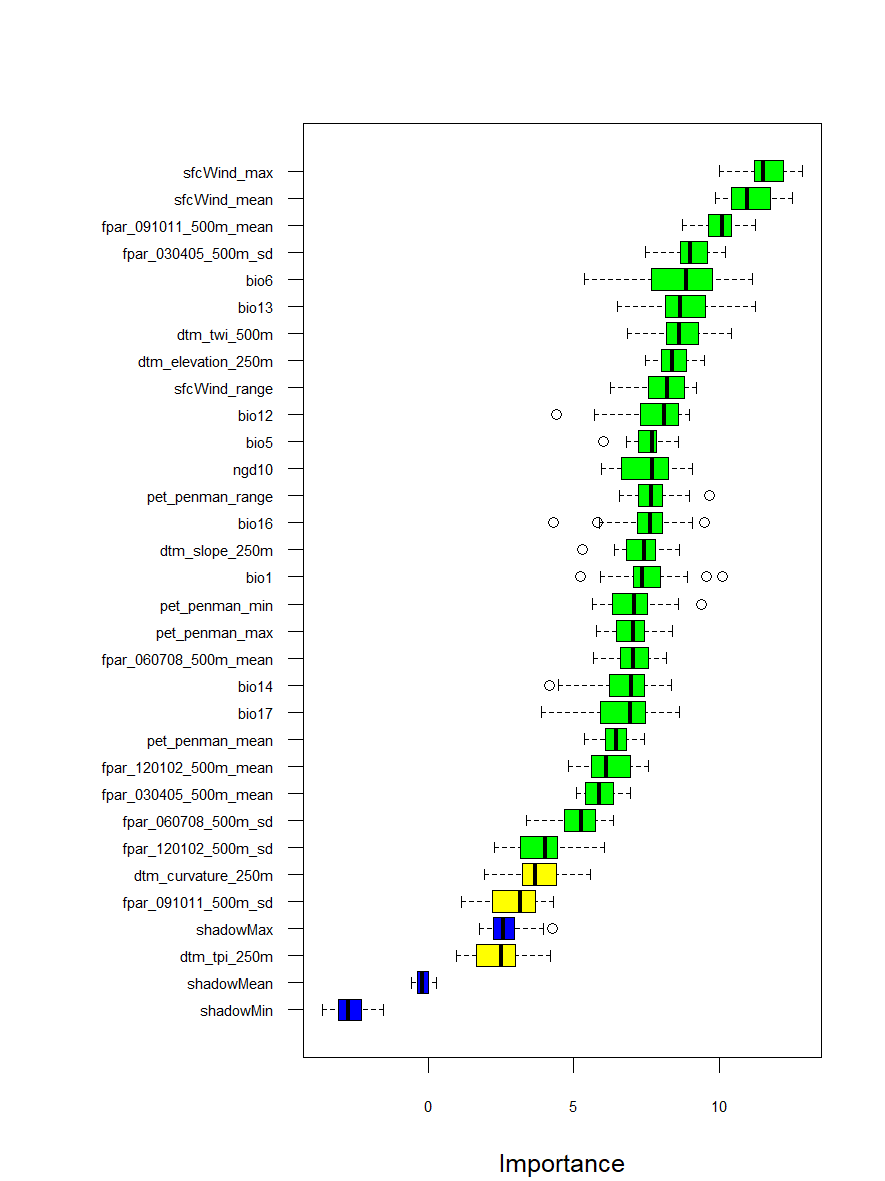
\includegraphics[width=12.29in]{images/module3/boruta_SOC} \caption{Boruta feature selection for SOC. Green = confirmed, red = rejected, yellow = tentative, blue = shadow variables.}\label{fig:boruta-plot}
\end{figure}

\begin{Shaded}
\begin{Highlighting}[]
\NormalTok{selected\_features }\OtherTok{\textless{}{-}} \FunctionTok{getSelectedAttributes}\NormalTok{(boruta\_result, }\AttributeTok{withTentative =} \ConstantTok{TRUE}\NormalTok{)}
\end{Highlighting}
\end{Shaded}

\texttt{getSelectedAttributes()} returns the names of confirmed predictors. Setting \texttt{withTentative\ =\ TRUE} also includes tentative ones --- a conservative choice that avoids discarding potentially useful variables.

\begin{quote}
\textbf{Feature selection in DSM: two schools of thought.} The field is divided on how to approach predictor selection. One tradition favours \emph{expert-guided selection}: the practitioner chooses covariates based on known soil-forming processes, keeping the predictor set small, interpretable, and grounded in pedological theory. The opposing view argues for \emph{data-driven inclusion}: feed all available covariates to the model and let the algorithm determine relevance --- a pragmatic position when the environmental drivers of a given soil property are poorly understood or when the goal is purely predictive accuracy. Boruta sits between these extremes: it is automated and data-driven, but its output can still be audited against expert knowledge (e.g.~rejecting a confirmed variable that has no plausible mechanistic link to the target, or overriding a rejection for a variable known to be important). In practice, the best approach depends on the study objective, the quality of the covariates, and the sample size available for model training.
\end{quote}

Here is the revised Section 6 with a proper QRF introduction:

\begin{center}\rule{0.5\linewidth}{0.5pt}\end{center}

\section*{Section 6 --- Train the Quantile Regression Forest model}\label{section-6-train-the-quantile-regression-forest-model}
\addcontentsline{toc}{section}{Section 6 --- Train the Quantile Regression Forest model}

\subsection*{6.1 From Random Forest to Quantile Regression Forest}\label{from-random-forest-to-quantile-regression-forest}
\addcontentsline{toc}{subsection}{6.1 From Random Forest to Quantile Regression Forest}

A standard Random Forest predicts the \textbf{expected value} (the mean) of the target variable at each new location. Each tree in the forest produces an estimate, and the final prediction is their average. This single number is useful, but it hides something important: it tells us \emph{what} the model predicts, but not \emph{how confident} we should be in that prediction.

\textbf{Quantile Regression Forest (QRF)} solves this by changing what each tree stores at its terminal nodes. Instead of keeping only the mean of the training observations that fall into a leaf, QRF retains \emph{all individual values}. This seemingly small change has a powerful consequence: at any new location, the model can reconstruct the full conditional distribution of the target --- not just its centre, but its spread, its skewness, and any quantile of interest.

In practice, this means QRF can produce \textbf{prediction intervals}. Rather than saying ``SOC here is 25 g kg⁻¹'', the model can say ``SOC here is 25 g kg⁻¹, and there is a 90\% probability it falls between 18 and 34 g kg⁻¹''. A narrow interval signals high confidence; a wide interval is the model's way of saying, transparently, that the environmental conditions at that location are poorly represented in the training data or that the local signal is inherently noisy.

Applied across the entire study area, this produces two complementary maps: a \textbf{mean prediction map} (the best estimate of SOC) and an \textbf{uncertainty map} (the conditional standard deviation, σ). Together they operationalise the Universal Model of Soil Variation introduced in Part I: ẑ(s) = m(s) ± σ(s). The uncertainty map is not a by-product --- it is a primary output that guides interpretation, identifies where additional sampling is most needed, and supports risk-aware decision making.

The \texttt{ranger} package makes QRF computationally feasible at the scale of regional DSM studies. Enabling it requires a single argument: \texttt{quantreg\ =\ TRUE}.

\subsection*{6.2 Cross-validation setup}\label{cross-validation-setup}
\addcontentsline{toc}{subsection}{6.2 Cross-validation setup}

Before training, we define how the model will be evaluated during hyperparameter tuning. Repeated k-fold cross-validation splits the dataset into \emph{k} folds, trains on \emph{k} − 1 and tests on the held-out fold, then repeats the whole cycle several times to reduce variance in the performance estimate.

\begin{Shaded}
\begin{Highlighting}[]
\NormalTok{cv\_control }\OtherTok{\textless{}{-}} \FunctionTok{trainControl}\NormalTok{(}
  \AttributeTok{method =} \StringTok{"repeatedcv"}\NormalTok{,}
  \AttributeTok{number =} \DecValTok{5}\NormalTok{,}
  \AttributeTok{repeats =} \DecValTok{5}\NormalTok{,}
  \AttributeTok{savePredictions =} \ConstantTok{TRUE}
\NormalTok{)}
\end{Highlighting}
\end{Shaded}

\texttt{savePredictions\ =\ TRUE} stores the out-of-fold predictions for every hyperparameter combination, which we will use in Section 7 to compute validation metrics without re-running the model.

\begin{quote}
\textbf{Limitation: standard CV assumes spatial independence.} Random fold assignment means a training fold and its test fold may contain samples that are geographically close, allowing the model to exploit spatial autocorrelation. This leads to over-optimistic accuracy estimates. Spatial cross-validation (e.g.~\texttt{CAST::CreateSpacetimeFolds()}) addresses this by grouping spatially proximate samples into the same fold. For this training exercise we use standard CV; keep this limitation in mind when interpreting results.
\end{quote}

\subsection*{6.3 Hyperparameter grid}\label{hyperparameter-grid}
\addcontentsline{toc}{subsection}{6.3 Hyperparameter grid}

\begin{longtable}[]{@{}
  >{\raggedright\arraybackslash}p{(\linewidth - 2\tabcolsep) * \real{0.5500}}
  >{\raggedright\arraybackslash}p{(\linewidth - 2\tabcolsep) * \real{0.4500}}@{}}
\toprule\noalign{}
\begin{minipage}[b]{\linewidth}\raggedright
Parameter
\end{minipage} & \begin{minipage}[b]{\linewidth}\raggedright
Meaning
\end{minipage} \\
\midrule\noalign{}
\endhead
\bottomrule\noalign{}
\endlastfoot
\textbf{mtry} & Number of covariates randomly sampled at each split \\
\textbf{min.node.size} & Minimum number of observations in a terminal node \\
\textbf{splitrule} & Split criterion: \texttt{variance} (standard RF) or \texttt{extratrees} (random splits --- faster, sometimes more accurate) \\
\end{longtable}

\begin{Shaded}
\begin{Highlighting}[]
\NormalTok{mtry\_base }\OtherTok{\textless{}{-}} \FunctionTok{round}\NormalTok{(}\FunctionTok{length}\NormalTok{(selected\_features) }\SpecialCharTok{/} \DecValTok{3}\NormalTok{)}
\NormalTok{tune\_grid }\OtherTok{\textless{}{-}} \FunctionTok{expand.grid}\NormalTok{(}
  \AttributeTok{mtry          =} \FunctionTok{c}\NormalTok{(mtry\_base }\SpecialCharTok{{-}} \FunctionTok{round}\NormalTok{(mtry\_base }\SpecialCharTok{/} \DecValTok{2}\NormalTok{),}
\NormalTok{                    mtry\_base,}
\NormalTok{                    mtry\_base }\SpecialCharTok{+} \FunctionTok{round}\NormalTok{(mtry\_base }\SpecialCharTok{/} \DecValTok{2}\NormalTok{)),}
  \AttributeTok{min.node.size =} \DecValTok{5}\NormalTok{,}
  \AttributeTok{splitrule     =} \FunctionTok{c}\NormalTok{(}\StringTok{"variance"}\NormalTok{, }\StringTok{"extratrees"}\NormalTok{)}
\NormalTok{)}
\end{Highlighting}
\end{Shaded}

\texttt{mtry} is initialised around the rule-of-thumb p/3 (where p is the number of selected features) and explored at three levels. \texttt{expand.grid()} produces every combination, yielding six candidate configurations.

\subsection*{6.4 Train the model}\label{train-the-model}
\addcontentsline{toc}{subsection}{6.4 Train the model}

\begin{Shaded}
\begin{Highlighting}[]
\NormalTok{model }\OtherTok{\textless{}{-}}\NormalTok{ caret}\SpecialCharTok{::}\FunctionTok{train}\NormalTok{(}
  \AttributeTok{y           =}\NormalTok{ d[, target],}
  \AttributeTok{x           =}\NormalTok{ d[, selected\_features],}
  \AttributeTok{method      =} \StringTok{"ranger"}\NormalTok{,}
  \AttributeTok{quantreg    =} \ConstantTok{TRUE}\NormalTok{,}
  \AttributeTok{importance  =} \StringTok{"permutation"}\NormalTok{,}
  \AttributeTok{trControl   =}\NormalTok{ cv\_control,}
  \AttributeTok{tuneGrid    =}\NormalTok{ tune\_grid,}
  \AttributeTok{num.threads =} \FunctionTok{max}\NormalTok{(}\DecValTok{1}\NormalTok{, parallel}\SpecialCharTok{::}\FunctionTok{detectCores}\NormalTok{() }\SpecialCharTok{{-}} \DecValTok{1}\NormalTok{)}
\NormalTok{)}

\NormalTok{model}
\NormalTok{model}\SpecialCharTok{$}\NormalTok{bestTune}
\end{Highlighting}
\end{Shaded}

\texttt{importance\ =\ "permutation"} measures how much accuracy drops when each predictor is randomly shuffled --- a reliable, model-agnostic importance measure. \texttt{num.threads} uses all but one CPU core; adjust downward if the machine is needed for other tasks during training.

\begin{figure}
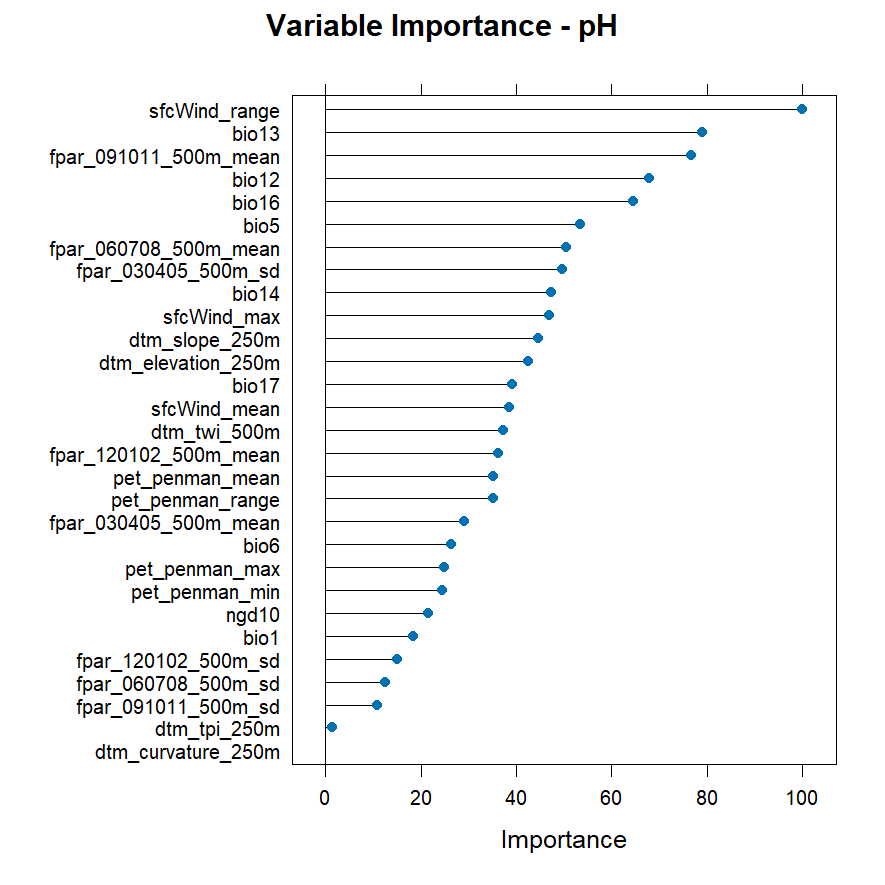
\includegraphics[width=12.29in]{images/module3/varImp_SOC} \caption{Permutation-based variable importance for the SOC model. Longer bars indicate stronger predictive contribution.}\label{fig:varimp-plot}
\end{figure}

Variable importance ranks predictors by their contribution to model accuracy. In SOC models, climate and vegetation indices (FPAR) typically dominate, while terrain attributes play a secondary role --- though this balance varies by region and target depth.

\section*{Section 7 --- Accuracy assessment}\label{section-7-accuracy-assessment}
\addcontentsline{toc}{section}{Section 7 --- Accuracy assessment}

Cross-validation accuracy is extracted from the predictions stored during training. Because \texttt{caret} evaluates every hyperparameter combination, we filter to the rows corresponding to the best configuration identified by \texttt{model\$bestTune}.

\begin{Shaded}
\begin{Highlighting}[]
\NormalTok{cv\_preds }\OtherTok{\textless{}{-}}\NormalTok{ model}\SpecialCharTok{$}\NormalTok{pred }\SpecialCharTok{\%\textgreater{}\%}
  \FunctionTok{filter}\NormalTok{(mtry          }\SpecialCharTok{==}\NormalTok{ model}\SpecialCharTok{$}\NormalTok{bestTune}\SpecialCharTok{$}\NormalTok{mtry,}
\NormalTok{         splitrule     }\SpecialCharTok{==}\NormalTok{ model}\SpecialCharTok{$}\NormalTok{bestTune}\SpecialCharTok{$}\NormalTok{splitrule,}
\NormalTok{         min.node.size }\SpecialCharTok{==}\NormalTok{ model}\SpecialCharTok{$}\NormalTok{bestTune}\SpecialCharTok{$}\NormalTok{min.node.size)}

\NormalTok{obs\_vals  }\OtherTok{\textless{}{-}}\NormalTok{ cv\_preds}\SpecialCharTok{$}\NormalTok{obs}
\NormalTok{pred\_vals }\OtherTok{\textless{}{-}}\NormalTok{ cv\_preds}\SpecialCharTok{$}\NormalTok{pred}
\end{Highlighting}
\end{Shaded}

The \texttt{eval()} function, loaded from \texttt{eval.RData}, implements the accuracy framework proposed by (\citeproc{ref-wadoux2021integrated}{\textbf{wadoux2021integrated?}}). It computes six complementary metrics from the vectors of observed (z) and predicted (ẑ) values:

\begin{Shaded}
\begin{Highlighting}[]
\FunctionTok{load}\NormalTok{(}\StringTok{"02\_scripts/module3/eval.RData"}\NormalTok{)}
\NormalTok{accuracy }\OtherTok{\textless{}{-}} \FunctionTok{eval}\NormalTok{(pred\_vals, obs\_vals)[, }\DecValTok{1}\SpecialCharTok{:}\DecValTok{6}\NormalTok{]}
\NormalTok{accuracy}
\end{Highlighting}
\end{Shaded}

\begin{table}

\caption{\label{tab:accuracy-table}Cross-validation accuracy metrics for the SOC model (Wadoux et al., 2021).}
\centering
\begin{tabular}[t]{r|r|r|r|r|r}
\hline
ME & MAE & RMSE & r & r2 & MEC\\
\hline
-0.02 & 0.5 & 0.72 & 0.7 & 0.49 & 0.49\\
\hline
\end{tabular}
\end{table}

\textbf{Mean Error (ME)} measures systematic bias --- the average signed difference between predictions and observations:

\[ME = \frac{1}{n}\sum_{i=1}^{n}(\hat{z}_i - z_i)\]

A positive ME means the model systematically over-predicts; a negative ME means it under-predicts. Values near zero are desirable, but ME alone can be misleading: large positive and negative errors can cancel out.

\textbf{Mean Absolute Error (MAE)} avoids cancellation by averaging the absolute deviations:

\[MAE = \frac{1}{n}\sum_{i=1}^{n}|\hat{z}_i - z_i|\]

MAE is in the same units as the target variable and is straightforward to interpret: on average, predictions deviate from observations by this amount.

\textbf{Root Mean Squared Error (RMSE)} also measures average error magnitude but penalises large errors more heavily than small ones by squaring the deviations before averaging:

\[RMSE = \sqrt{\frac{1}{n}\sum_{i=1}^{n}(\hat{z}_i - z_i)^2}\]

RMSE is more sensitive to outliers than MAE. When RMSE \textgreater\textgreater{} MAE, a few large errors dominate the total error budget. Comparing both metrics together reveals the error distribution.

\textbf{Pearson correlation coefficient (r)} measures the strength and direction of the linear relationship between observed and predicted values:

\[r = \frac{\sum_{i=1}^{n}(z_i - \bar{z})(\hat{z}_i - \bar{\hat{z}})}{\sqrt{\sum_{i=1}^{n}(z_i - \bar{z})^2 \cdot \sum_{i=1}^{n}(\hat{z}_i - \bar{\hat{z}})^2}}\]

Values range from −1 to 1. Note that r measures association, not agreement: a model that consistently predicts twice the observed value would have r = 1 but poor accuracy. It should always be read alongside bias metrics.

\textbf{Coefficient of determination (R²)} quantifies the proportion of variance in the observations explained by the model:

\[R^2 = 1 - \frac{\sum_{i=1}^{n}(z_i - \hat{z}_i)^2}{\sum_{i=1}^{n}(z_i - \bar{z})^2}\]

Unlike r, R² is sensitive to systematic bias. A model with no bias and perfect correlation yields R² = 1; a model that predicts the observed mean for every point yields R² = 0.

\textbf{Model Efficiency Coefficient (MEC)} --- also known as the Nash-Sutcliffe efficiency --- is the most demanding of the six metrics. It compares the model's squared errors against the squared deviations from the observed mean, i.e.~the error one would incur by always predicting \(\bar{z}\):

\[MEC = 1 - \frac{\sum_{i=1}^{n}(z_i - \hat{z}_i)^2}{\sum_{i=1}^{n}(z_i - \bar{z})^2}\]

MEC = 1 is a perfect model. MEC = 0 means the model is no better than simply predicting the mean everywhere. \textbf{MEC \textless{} 0} means the observed mean is a better predictor than the model --- a clear sign of model failure. MEC is particularly informative in DSM because it directly benchmarks the spatial model against the null case of no spatial structure.

\begin{quote}
\textbf{Tip:} In practice, a MEC above 0.5 is often considered acceptable for DSM models of highly variable soil properties like SOC. Values above 0.7 indicate good model skill. If MEC is close to zero or negative, revisit the covariate stack --- the predictors may not capture the main drivers of spatial variability at the target depth.
\end{quote}

\subsection*{Observed vs predicted plot}\label{observed-vs-predicted-plot}
\addcontentsline{toc}{subsection}{Observed vs predicted plot}

\begin{Shaded}
\begin{Highlighting}[]
\NormalTok{residuals }\OtherTok{\textless{}{-}} \FunctionTok{tibble}\NormalTok{(}\AttributeTok{Observed =}\NormalTok{ obs\_vals, }\AttributeTok{Predicted =}\NormalTok{ pred\_vals)}
\NormalTok{g\_scatter }\OtherTok{\textless{}{-}} \FunctionTok{ggplot}\NormalTok{(residuals, }\FunctionTok{aes}\NormalTok{(}\AttributeTok{x =}\NormalTok{ Observed, }\AttributeTok{y =}\NormalTok{ Predicted)) }\SpecialCharTok{+}
  \FunctionTok{geom\_point}\NormalTok{(}\AttributeTok{alpha =} \FloatTok{0.3}\NormalTok{) }\SpecialCharTok{+}
  \FunctionTok{geom\_abline}\NormalTok{(}\AttributeTok{slope =} \DecValTok{1}\NormalTok{, }\AttributeTok{intercept =} \DecValTok{0}\NormalTok{, }\AttributeTok{color =} \StringTok{"red"}\NormalTok{, }\AttributeTok{linewidth =} \DecValTok{1}\NormalTok{) }\SpecialCharTok{+}
  \FunctionTok{ylim}\NormalTok{(}\FunctionTok{c}\NormalTok{(}\FunctionTok{min}\NormalTok{(residuals}\SpecialCharTok{$}\NormalTok{Observed), }\FunctionTok{max}\NormalTok{(residuals}\SpecialCharTok{$}\NormalTok{Observed))) }\SpecialCharTok{+}
  \FunctionTok{theme}\NormalTok{(}\AttributeTok{aspect.ratio =} \DecValTok{1}\NormalTok{) }\SpecialCharTok{+}
  \FunctionTok{coord\_fixed}\NormalTok{() }\SpecialCharTok{+}
  \FunctionTok{labs}\NormalTok{(}\AttributeTok{title =} \FunctionTok{paste}\NormalTok{(}\StringTok{"Observed vs Predicted {-}"}\NormalTok{, target)) }\SpecialCharTok{+}
  \FunctionTok{theme\_minimal}\NormalTok{()}

\NormalTok{g\_scatter}
\end{Highlighting}
\end{Shaded}

\begin{figure}
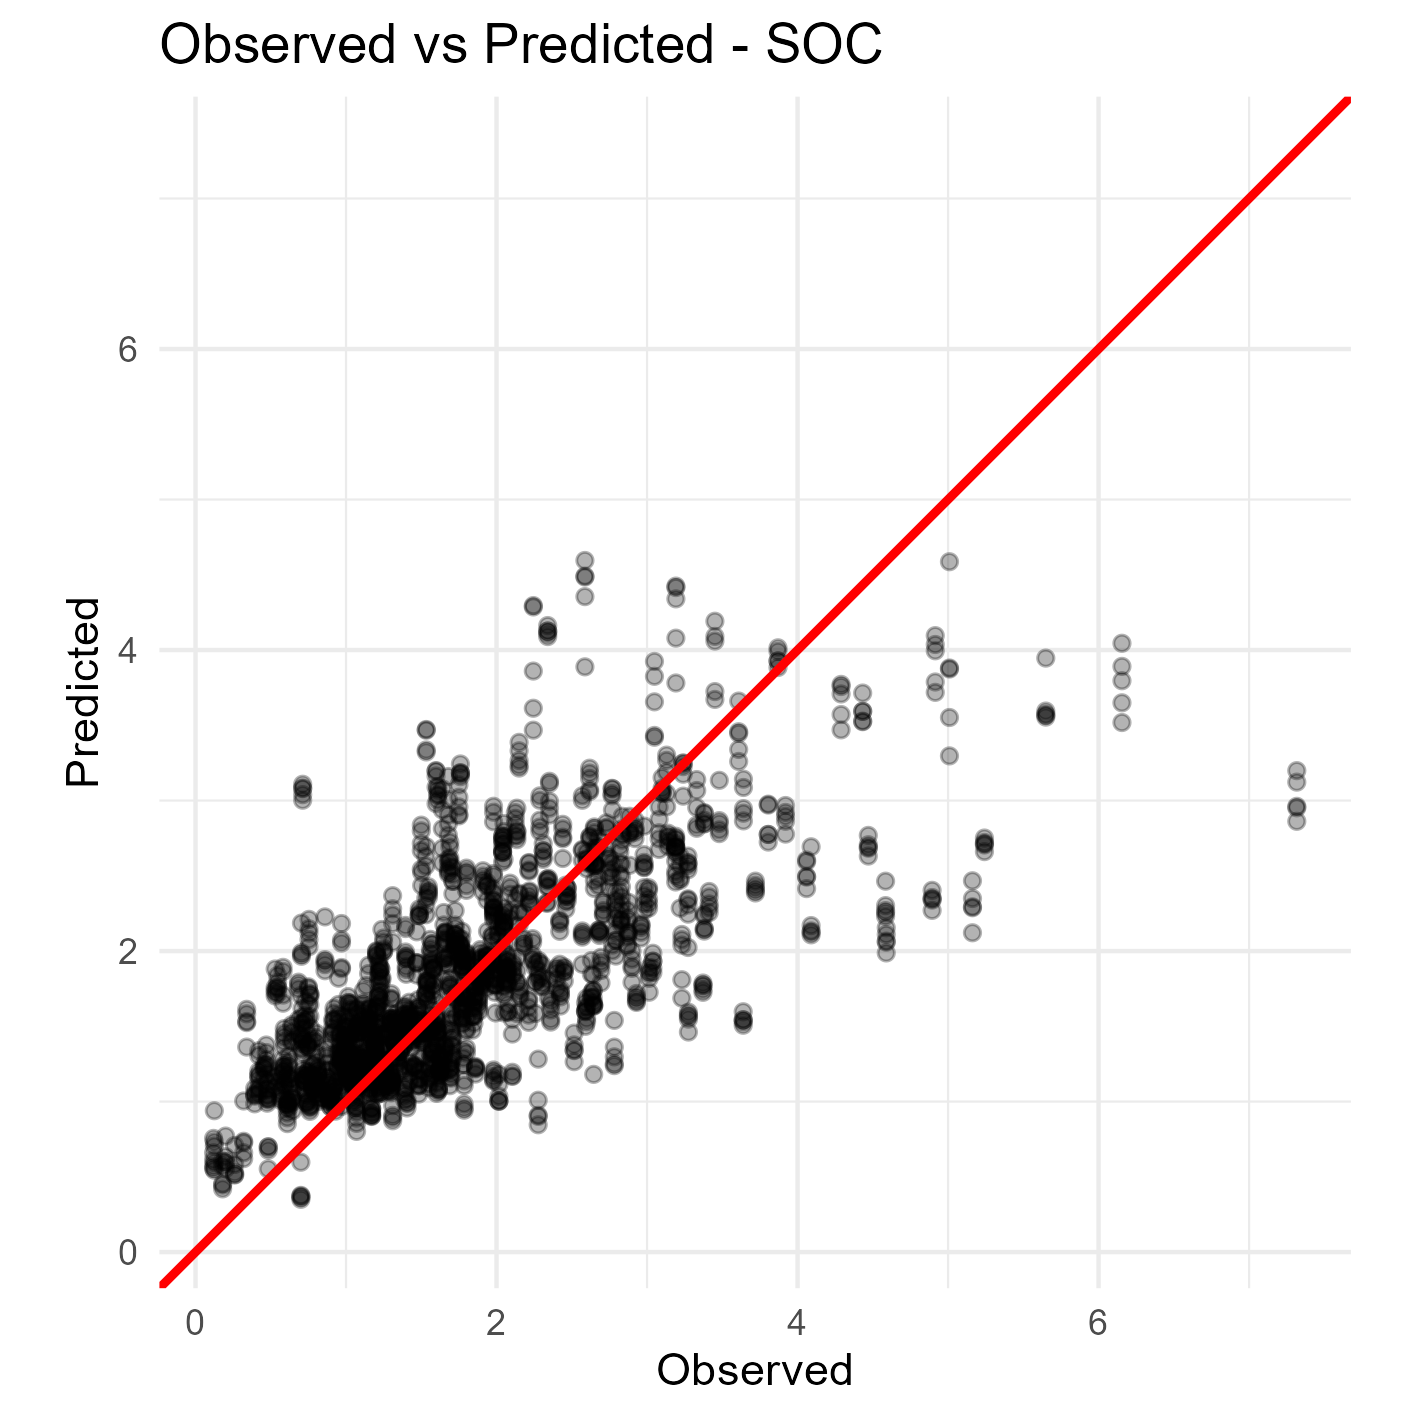
\includegraphics[width=19.68in]{images/module3/scatterplot_SOC} \caption{Observed vs predicted SOC values from cross-validation. The red line is the 1:1 line; a perfect model places all points on it.}\label{fig:scatter-plot}
\end{figure}

A common pattern in cross-validated scatterplots is \textbf{regression to the mean}: very high observed values tend to be under-predicted and very low values tend to be over-predicted. This reflects the model's limited ability to extrapolate beyond the range well-represented in the training data, and is expected behaviour rather than a model failure. Wide scatter at intermediate values indicates that the covariates do not fully capture local SOC variability at those concentrations.

\subsection*{Save outputs}\label{save-outputs}
\addcontentsline{toc}{subsection}{Save outputs}

\begin{Shaded}
\begin{Highlighting}[]
\FunctionTok{write\_csv}\NormalTok{(accuracy, }\StringTok{"03\_outputs/module3/validation/accuracy.csv"}\NormalTok{)}
\FunctionTok{saveRDS}\NormalTok{(model, }\FunctionTok{paste0}\NormalTok{(}\StringTok{"03\_outputs/module3/models/ranger\_model\_"}\NormalTok{, target, }\StringTok{".rds"}\NormalTok{))}
\end{Highlighting}
\end{Shaded}

\texttt{write\_csv()} saves the accuracy table for reporting and reproducibility. \texttt{saveRDS()} serialises the full caret model object --- including the trained ranger forest, CV results, and tuning history. Session 2 reloads it with \texttt{readRDS()} to run spatial prediction without retraining.

\begin{quote}
\textbf{Limitation:} Cross-validation accuracy reflects performance on the training dataset, not on locations that are environmentally different from the sampled area. If the study region contains landscapes that are underrepresented in the samples (e.g.~poorly drained soils, organic-rich wetland patches), the actual map error in those areas will be higher than the reported CV metrics suggest.
\end{quote}

\begin{center}\rule{0.5\linewidth}{0.5pt}\end{center}

\section*{SESSION 2: Spatial Prediction and Final Maps}\label{session-2-spatial-prediction-and-final-maps}
\addcontentsline{toc}{section}{SESSION 2: Spatial Prediction and Final Maps}

\begin{center}\rule{0.5\linewidth}{0.5pt}\end{center}

\section*{Reload the workspace}\label{reload-the-workspace}
\addcontentsline{toc}{section}{Reload the workspace}

Session 2 is designed to be \textbf{self-contained}: it reloads all necessary objects from disk so you can run spatial prediction independently, without re-running Session 1. This is important in practice --- model training can take hours, and you may want to experiment with prediction parameters without repeating the full workflow.

\begin{Shaded}
\begin{Highlighting}[]
\FunctionTok{library}\NormalTok{(tidyverse)}
\FunctionTok{library}\NormalTok{(caret)}
\FunctionTok{library}\NormalTok{(terra)}
\FunctionTok{library}\NormalTok{(ranger)}

\FunctionTok{Sys.setenv}\NormalTok{(}\AttributeTok{PROJ\_LIB =} \StringTok{""}\NormalTok{)}
\FunctionTok{Sys.setenv}\NormalTok{(}\AttributeTok{PROJ\_DATA =} \FunctionTok{system.file}\NormalTok{(}\StringTok{"proj"}\NormalTok{, }\AttributeTok{package =} \StringTok{"terra"}\NormalTok{))}

\FunctionTok{setwd}\NormalTok{(}\FunctionTok{dirname}\NormalTok{(rstudioapi}\SpecialCharTok{::}\FunctionTok{getActiveDocumentContext}\NormalTok{()}\SpecialCharTok{$}\NormalTok{path))}
\FunctionTok{setwd}\NormalTok{(}\StringTok{"../../"}\NormalTok{)}

\NormalTok{covs    }\OtherTok{\textless{}{-}} \FunctionTok{rast}\NormalTok{(}\StringTok{"01\_data/module3/Env\_Cov\_250m\_KANSAS.tif"}\NormalTok{)}
\NormalTok{cov\_names }\OtherTok{\textless{}{-}} \FunctionTok{names}\NormalTok{(covs)}
\NormalTok{target  }\OtherTok{\textless{}{-}} \StringTok{"SOC"}
\NormalTok{model   }\OtherTok{\textless{}{-}} \FunctionTok{readRDS}\NormalTok{(}\FunctionTok{paste0}\NormalTok{(}\StringTok{"03\_outputs/module3/models/ranger\_model\_"}\NormalTok{, target, }\StringTok{".rds"}\NormalTok{))}
\end{Highlighting}
\end{Shaded}

\texttt{readRDS()} reconstructs the full caret model object exactly as it was when saved, including the trained ranger forest and the optimal hyperparameter configuration.

\section*{Section 8 --- Spatial prediction (tiled)}\label{section-8-spatial-prediction-tiled}
\addcontentsline{toc}{section}{Section 8 --- Spatial prediction (tiled)}

Predicting SOC across the full study area requires applying the model to every pixel of the covariate stack. For large rasters this is memory-intensive: loading the full stack and computing predictions simultaneously can exhaust available RAM. The solution is \textbf{tiled prediction} --- splitting the study area into a grid of smaller tiles, predicting each tile independently, and mosaicking the results at the end.

\subsection*{8.1 Create tile grid}\label{create-tile-grid}
\addcontentsline{toc}{subsection}{8.1 Create tile grid}

\begin{Shaded}
\begin{Highlighting}[]
\NormalTok{r    }\OtherTok{\textless{}{-}}\NormalTok{ covs[[}\DecValTok{1}\NormalTok{]]}
\NormalTok{t    }\OtherTok{\textless{}{-}} \FunctionTok{rast}\NormalTok{(}\AttributeTok{nrows =} \DecValTok{5}\NormalTok{, }\AttributeTok{ncols =} \DecValTok{10}\NormalTok{, }\AttributeTok{extent =} \FunctionTok{ext}\NormalTok{(r), }\AttributeTok{crs =} \FunctionTok{crs}\NormalTok{(r))}
\NormalTok{tile }\OtherTok{\textless{}{-}} \FunctionTok{makeTiles}\NormalTok{(r, t, }\AttributeTok{overwrite =} \ConstantTok{TRUE}\NormalTok{,}
                  \AttributeTok{filename =} \StringTok{"03\_outputs/module3/tiles/tiles.tif"}\NormalTok{)}

\FunctionTok{rast}\NormalTok{(tile[}\DecValTok{1}\NormalTok{]) }\SpecialCharTok{\%\textgreater{}\%}\NormalTok{ plot}
\end{Highlighting}
\end{Shaded}

\texttt{makeTiles()} divides the extent of a reference raster (\texttt{r}, here the first covariate layer) into a grid defined by \texttt{t} --- a template raster with 5 rows and 10 columns of tiles. It writes one small \texttt{.tif} per tile and returns a vector of file paths. The grid here produces 50 tiles; each tile is a manageable chunk of the full extent.

\begin{quote}
\textbf{Tip:} The right number of tiles depends on your available RAM and the number of covariate layers. A rough guide: if \texttt{nlyr(covs)\ ×\ nrow\_tile\ ×\ ncol\_tile\ ×\ 4\ bytes} exceeds \textasciitilde60\% of your free RAM, increase the number of tiles. You can inspect tile dimensions with \texttt{rast(tile{[}1{]})} before committing to the full prediction loop.
\end{quote}

\subsection*{8.2 Prepare model for prediction}\label{prepare-model-for-prediction}
\addcontentsline{toc}{subsection}{8.2 Prepare model for prediction}

\begin{Shaded}
\begin{Highlighting}[]
\NormalTok{ranger\_model }\OtherTok{\textless{}{-}}\NormalTok{ model}\SpecialCharTok{$}\NormalTok{finalModel}

\NormalTok{pfun }\OtherTok{\textless{}{-}} \ControlFlowTok{function}\NormalTok{(...) \{}
  \FunctionTok{predict}\NormalTok{(...)}\SpecialCharTok{$}\NormalTok{predictions }\SpecialCharTok{|\textgreater{}} \FunctionTok{t}\NormalTok{()}
\NormalTok{\}}

\NormalTok{gdal\_opts }\OtherTok{\textless{}{-}} \FunctionTok{c}\NormalTok{(}\StringTok{"COMPRESS=LZW"}\NormalTok{, }\StringTok{"TILED=YES"}\NormalTok{, }\StringTok{"BIGTIFF=IF\_SAFER"}\NormalTok{)}
\end{Highlighting}
\end{Shaded}

\texttt{model\$finalModel} extracts the raw ranger model from the caret wrapper --- needed because \texttt{terra::interpolate()} calls \texttt{predict()} directly on the model object. The custom prediction function \texttt{pfun} wraps this call and transposes the output matrix (\texttt{t()}): ranger returns quantile predictions in a format where rows are quantiles and columns are pixels, but terra expects the opposite orientation.

\texttt{gdal\_opts} sets three GDAL write options applied when saving rasters to disk: LZW lossless compression reduces file size significantly, tiled storage accelerates partial reads (e.g.~when zooming in a GIS), and \texttt{BIGTIFF=IF\_SAFER} automatically uses the BigTIFF format if the output exceeds 4 GB.

\subsection*{8.3 Prediction for one tile}\label{prediction-for-one-tile}
\addcontentsline{toc}{subsection}{8.3 Prediction for one tile}

Before running the full loop, we test the prediction pipeline on a single tile. This lets you verify that the output looks correct and estimate processing time per tile.

\begin{Shaded}
\begin{Highlighting}[]
\NormalTok{t1       }\OtherTok{\textless{}{-}} \FunctionTok{rast}\NormalTok{(tile[}\DecValTok{1}\NormalTok{])}
\NormalTok{covs\_t1  }\OtherTok{\textless{}{-}} \FunctionTok{crop}\NormalTok{(covs, t1)}

\NormalTok{pred\_mean\_t1 }\OtherTok{\textless{}{-}}\NormalTok{ terra}\SpecialCharTok{::}\FunctionTok{interpolate}\NormalTok{(covs\_t1,}
                                   \AttributeTok{model =}\NormalTok{ ranger\_model,}
                                   \AttributeTok{fun   =}\NormalTok{ pfun,}
                                   \AttributeTok{na.rm =} \ConstantTok{TRUE}\NormalTok{,}
                                   \AttributeTok{type  =} \StringTok{"quantiles"}\NormalTok{,}
                                   \AttributeTok{what  =}\NormalTok{ mean)}

\NormalTok{pred\_sd\_t1   }\OtherTok{\textless{}{-}}\NormalTok{ terra}\SpecialCharTok{::}\FunctionTok{interpolate}\NormalTok{(covs\_t1,}
                                   \AttributeTok{model =}\NormalTok{ ranger\_model,}
                                   \AttributeTok{fun   =}\NormalTok{ pfun,}
                                   \AttributeTok{na.rm =} \ConstantTok{TRUE}\NormalTok{,}
                                   \AttributeTok{type  =} \StringTok{"quantiles"}\NormalTok{,}
                                   \AttributeTok{what  =}\NormalTok{ sd)}

\NormalTok{pred\_cv\_t1 }\OtherTok{\textless{}{-}}\NormalTok{ pred\_sd\_t1 }\SpecialCharTok{/}\NormalTok{ pred\_mean\_t1}

\FunctionTok{mapview}\NormalTok{(pred\_mean\_t1)}
\end{Highlighting}
\end{Shaded}

\texttt{terra::interpolate()} applies the model to every pixel of the covariate tile. The \texttt{what} argument controls which summary of the quantile distribution is computed: \texttt{what\ =\ mean} returns the conditional mean (the best-estimate prediction map), and \texttt{what\ =\ sd} returns the conditional standard deviation (the uncertainty map). These correspond directly to m(s) and σ(s) in the Universal Model of Soil Variation.

\begin{figure}
\centering
\pandocbounded{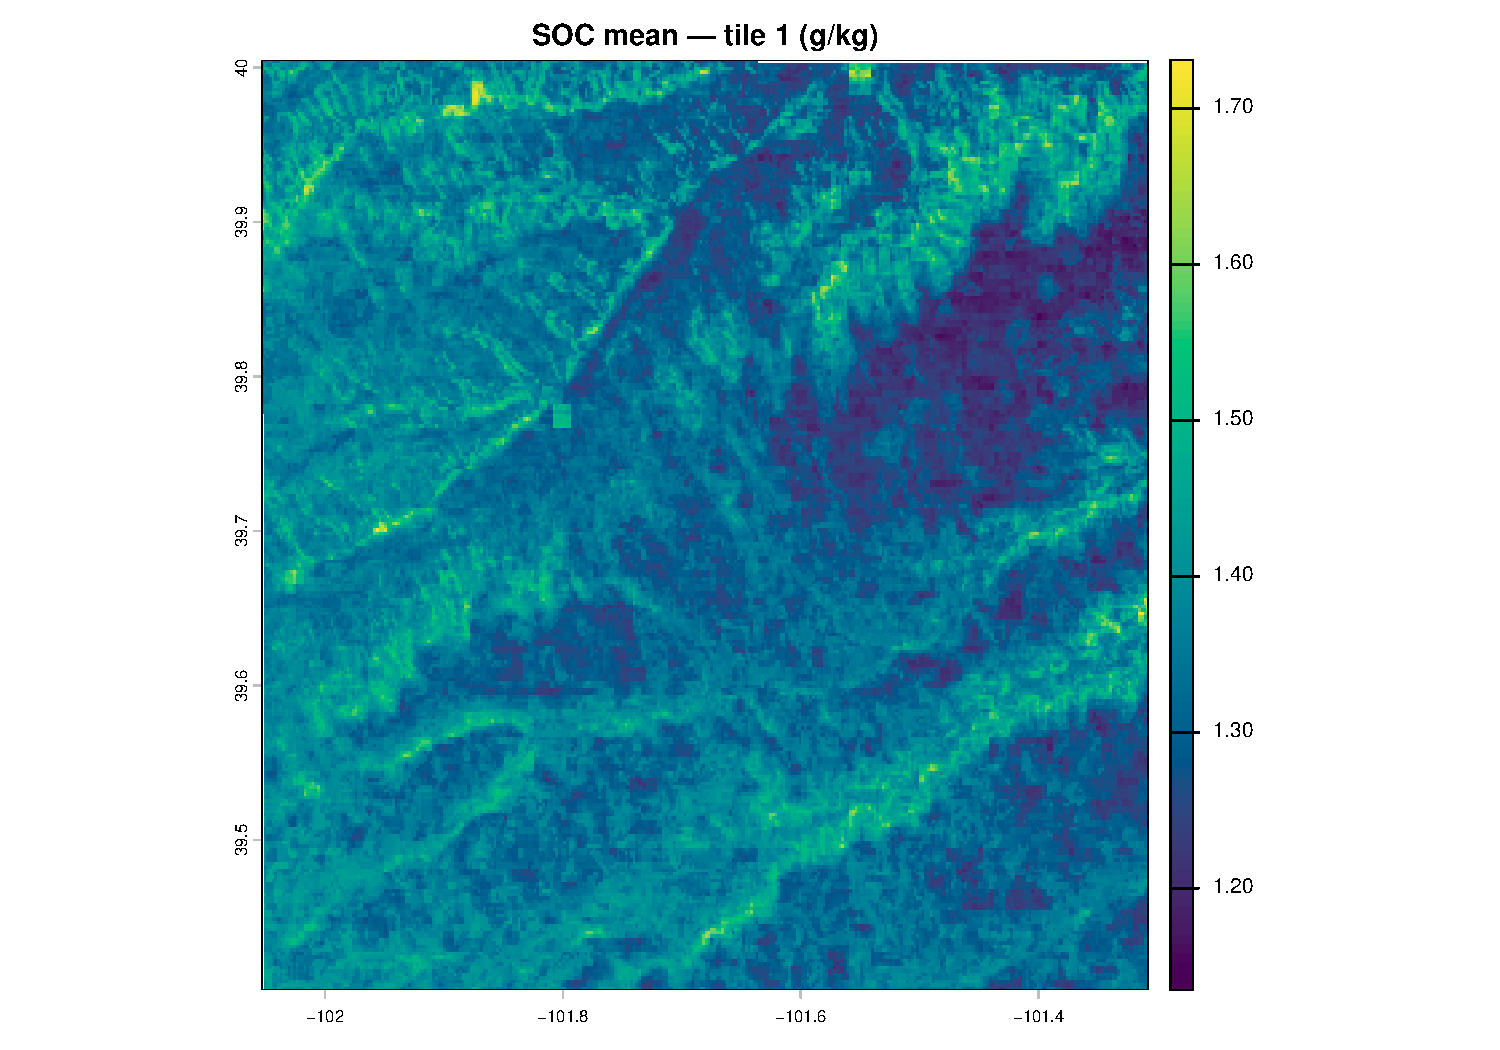
\includegraphics[keepaspectratio]{SoilFER-Integrated-soil-information-for-decision-making_files/figure-latex/tile1-mean-1.pdf}}
\caption{\label{fig:tile1-mean}SOC mean prediction for tile 1 (g/kg).}
\end{figure}

\begin{figure}
\centering
\pandocbounded{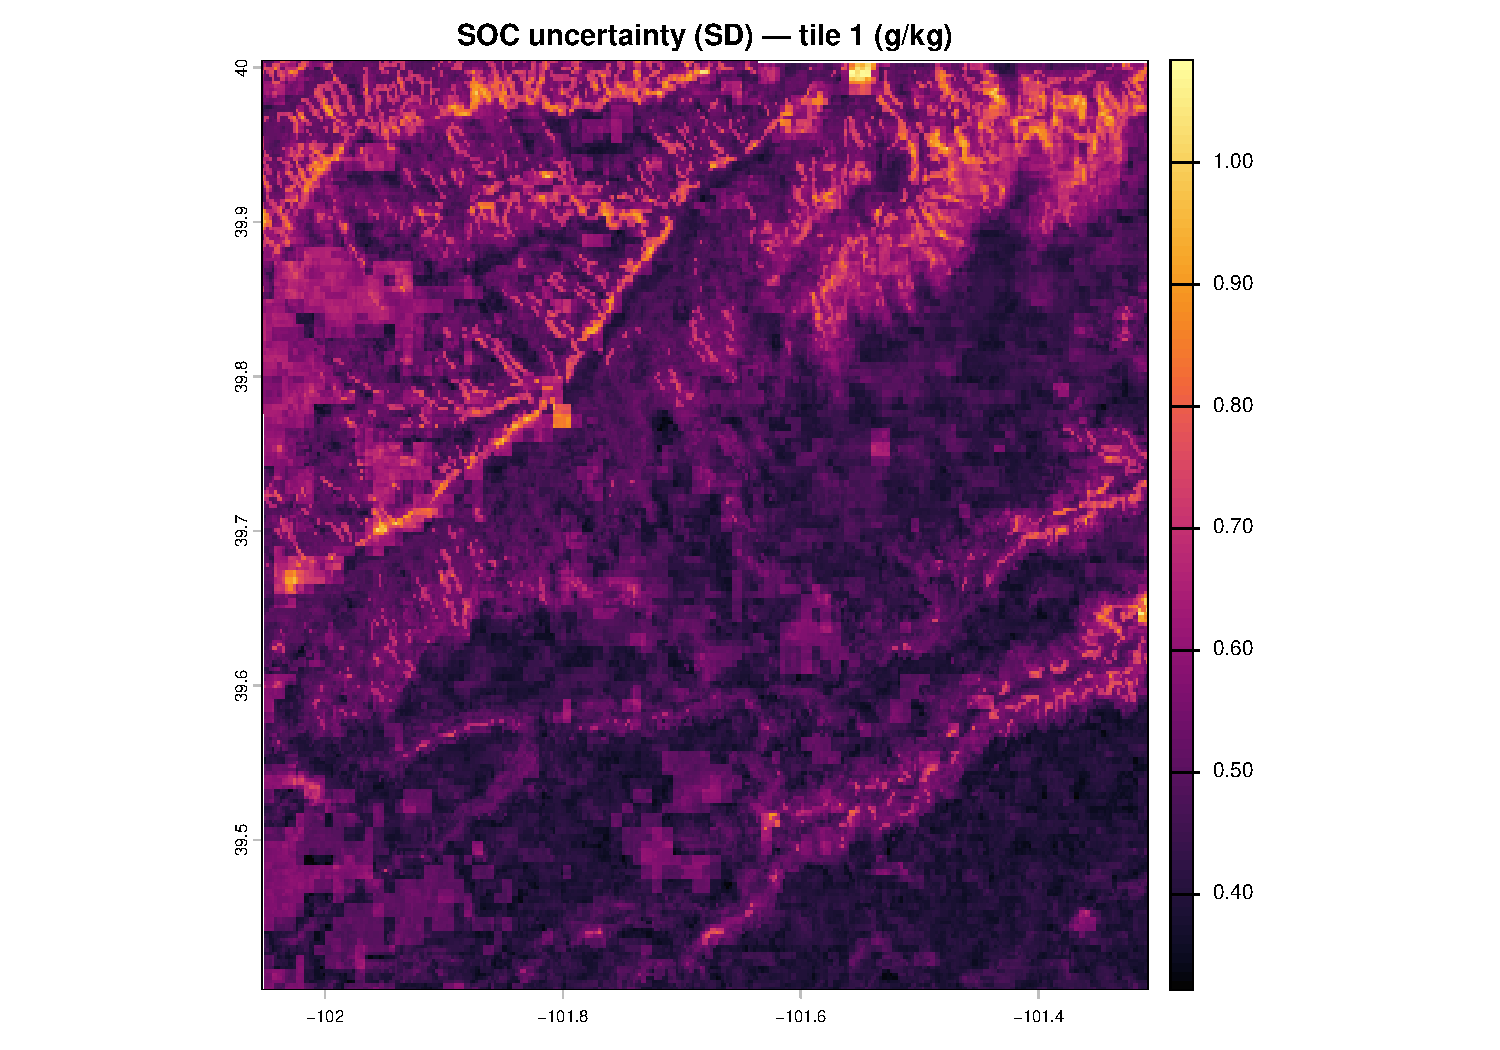
\includegraphics[keepaspectratio]{SoilFER-Integrated-soil-information-for-decision-making_files/figure-latex/tile1-sd-1.pdf}}
\caption{\label{fig:tile1-sd}SOC prediction uncertainty (SD) for tile 1 (g/kg).}
\end{figure}

\begin{quote}
\textbf{Reading the uncertainty map:} high SD values indicate locations where the model is less confident --- typically at the extremes of the environmental gradient, in areas with few nearby training samples, or where the covariate combination is unlike anything seen during training. These areas should be prioritised for additional soil sampling in future surveys.
\end{quote}

\subsection*{8.4 Prediction at all tiles}\label{prediction-at-all-tiles}
\addcontentsline{toc}{subsection}{8.4 Prediction at all tiles}

Once the single-tile test is satisfactory, run the loop over all tiles:

\begin{Shaded}
\begin{Highlighting}[]
\ControlFlowTok{for}\NormalTok{ (j }\ControlFlowTok{in} \FunctionTok{seq\_along}\NormalTok{(tile)) \{}
  \FunctionTok{print}\NormalTok{(}\FunctionTok{paste}\NormalTok{(}\StringTok{"Processing tile"}\NormalTok{, j, }\StringTok{"of"}\NormalTok{, }\FunctionTok{length}\NormalTok{(tile)))}

\NormalTok{  t\_j        }\OtherTok{\textless{}{-}} \FunctionTok{rast}\NormalTok{(tile[j])}
\NormalTok{  covs\_tile  }\OtherTok{\textless{}{-}} \FunctionTok{crop}\NormalTok{(covs, t\_j)}

\NormalTok{  mean\_file }\OtherTok{\textless{}{-}} \FunctionTok{paste0}\NormalTok{(}\StringTok{"03\_outputs/module3/tiles/"}\NormalTok{, target, }\StringTok{"\_mean\_"}\NormalTok{, j, }\StringTok{".tif"}\NormalTok{)}
\NormalTok{  terra}\SpecialCharTok{::}\FunctionTok{interpolate}\NormalTok{(covs\_tile, }\AttributeTok{model =}\NormalTok{ ranger\_model, }\AttributeTok{fun =}\NormalTok{ pfun,}
                     \AttributeTok{na.rm =} \ConstantTok{TRUE}\NormalTok{, }\AttributeTok{type =} \StringTok{"quantiles"}\NormalTok{, }\AttributeTok{what =}\NormalTok{ mean,}
                     \AttributeTok{filename =}\NormalTok{ mean\_file, }\AttributeTok{overwrite =} \ConstantTok{TRUE}\NormalTok{,}
                     \AttributeTok{wopt =} \FunctionTok{list}\NormalTok{(}\AttributeTok{datatype =} \StringTok{"FLT4S"}\NormalTok{, }\AttributeTok{gdal =}\NormalTok{ gdal\_opts))}

\NormalTok{  sd\_file }\OtherTok{\textless{}{-}} \FunctionTok{paste0}\NormalTok{(}\StringTok{"03\_outputs/module3/tiles/"}\NormalTok{, target, }\StringTok{"\_sd\_"}\NormalTok{, j, }\StringTok{".tif"}\NormalTok{)}
\NormalTok{  terra}\SpecialCharTok{::}\FunctionTok{interpolate}\NormalTok{(covs\_tile, }\AttributeTok{model =}\NormalTok{ ranger\_model, }\AttributeTok{fun =}\NormalTok{ pfun,}
                     \AttributeTok{na.rm =} \ConstantTok{TRUE}\NormalTok{, }\AttributeTok{type =} \StringTok{"quantiles"}\NormalTok{, }\AttributeTok{what =}\NormalTok{ sd,}
                     \AttributeTok{filename =}\NormalTok{ sd\_file, }\AttributeTok{overwrite =} \ConstantTok{TRUE}\NormalTok{,}
                     \AttributeTok{wopt =} \FunctionTok{list}\NormalTok{(}\AttributeTok{datatype =} \StringTok{"FLT4S"}\NormalTok{, }\AttributeTok{gdal =}\NormalTok{ gdal\_opts))}
\NormalTok{\}}
\end{Highlighting}
\end{Shaded}

\texttt{paste0()} constructs the output file path dynamically for each tile index \texttt{j}. Writing directly to disk with \texttt{filename\ =} means terra never holds the full prediction in memory --- each tile is computed and saved before moving to the next.

\begin{quote}
\textbf{Processing time:} with 50 tiles and a moderately sized training dataset, this loop typically takes 20--60 minutes depending on the number of trees, the tile size, and available CPU cores. Note that \texttt{terra::interpolate()} is single-threaded per tile; running tiles in parallel requires an explicit parallelisation wrapper (e.g.~\texttt{foreach} + \texttt{doParallel}).
\end{quote}

\section*{Section 9 --- Mosaic tiles into final maps}\label{section-9-mosaic-tiles-into-final-maps}
\addcontentsline{toc}{section}{Section 9 --- Mosaic tiles into final maps}

\begin{Shaded}
\begin{Highlighting}[]
\NormalTok{mean\_tiles   }\OtherTok{\textless{}{-}} \FunctionTok{list.files}\NormalTok{(}\StringTok{"03\_outputs/module3/tiles/"}\NormalTok{,}
                            \AttributeTok{pattern    =} \FunctionTok{paste0}\NormalTok{(}\StringTok{"\^{}"}\NormalTok{, target, }\StringTok{"\_mean\_.*}\SpecialCharTok{\textbackslash{}\textbackslash{}}\StringTok{.tif$"}\NormalTok{),}
                            \AttributeTok{full.names =} \ConstantTok{TRUE}\NormalTok{)}

\NormalTok{mean\_rasters }\OtherTok{\textless{}{-}} \FunctionTok{lapply}\NormalTok{(mean\_tiles, rast)}
\NormalTok{pred\_mean    }\OtherTok{\textless{}{-}} \FunctionTok{mosaic}\NormalTok{(}\FunctionTok{sprc}\NormalTok{(mean\_rasters))}
\FunctionTok{names}\NormalTok{(pred\_mean) }\OtherTok{\textless{}{-}} \FunctionTok{paste0}\NormalTok{(target, }\StringTok{"\_mean"}\NormalTok{)}

\FunctionTok{writeRaster}\NormalTok{(pred\_mean,}
            \FunctionTok{paste0}\NormalTok{(}\StringTok{"03\_outputs/module3/maps/mean\_"}\NormalTok{, target, }\StringTok{".tif"}\NormalTok{),}
            \AttributeTok{overwrite =} \ConstantTok{TRUE}\NormalTok{,}
            \AttributeTok{wopt =} \FunctionTok{list}\NormalTok{(}\AttributeTok{datatype =} \StringTok{"FLT4S"}\NormalTok{, }\AttributeTok{gdal =}\NormalTok{ gdal\_opts))}

\NormalTok{sd\_tiles   }\OtherTok{\textless{}{-}} \FunctionTok{list.files}\NormalTok{(}\StringTok{"03\_outputs/module3/tiles/"}\NormalTok{,}
                          \AttributeTok{pattern    =} \FunctionTok{paste0}\NormalTok{(}\StringTok{"\^{}"}\NormalTok{, target, }\StringTok{"\_sd\_.*}\SpecialCharTok{\textbackslash{}\textbackslash{}}\StringTok{.tif$"}\NormalTok{),}
                          \AttributeTok{full.names =} \ConstantTok{TRUE}\NormalTok{)}

\NormalTok{sd\_rasters }\OtherTok{\textless{}{-}} \FunctionTok{lapply}\NormalTok{(sd\_tiles, rast)}
\NormalTok{pred\_sd    }\OtherTok{\textless{}{-}} \FunctionTok{mosaic}\NormalTok{(}\FunctionTok{sprc}\NormalTok{(sd\_rasters))}
\FunctionTok{names}\NormalTok{(pred\_sd) }\OtherTok{\textless{}{-}} \FunctionTok{paste0}\NormalTok{(target, }\StringTok{"\_sd"}\NormalTok{)}

\FunctionTok{writeRaster}\NormalTok{(pred\_sd,}
            \FunctionTok{paste0}\NormalTok{(}\StringTok{"03\_outputs/module3/maps/sd\_"}\NormalTok{, target, }\StringTok{".tif"}\NormalTok{),}
            \AttributeTok{overwrite =} \ConstantTok{TRUE}\NormalTok{,}
            \AttributeTok{wopt =} \FunctionTok{list}\NormalTok{(}\AttributeTok{datatype =} \StringTok{"FLT4S"}\NormalTok{, }\AttributeTok{gdal =}\NormalTok{ gdal\_opts))}

\FunctionTok{plot}\NormalTok{(pred\_mean, }\AttributeTok{main =} \FunctionTok{paste}\NormalTok{(}\StringTok{"Mean"}\NormalTok{, target), }\AttributeTok{col =} \FunctionTok{hcl.colors}\NormalTok{(}\DecValTok{100}\NormalTok{, }\StringTok{"Viridis"}\NormalTok{))}
\FunctionTok{plot}\NormalTok{(pred\_sd,   }\AttributeTok{main =} \FunctionTok{paste}\NormalTok{(}\StringTok{"SD"}\NormalTok{,   target), }\AttributeTok{col =} \FunctionTok{hcl.colors}\NormalTok{(}\DecValTok{100}\NormalTok{, }\StringTok{"Inferno"}\NormalTok{))}
\end{Highlighting}
\end{Shaded}

\texttt{list.files()} with a regular expression pattern collects all mean (or SD) tile files in the correct order. \texttt{sprc()} wraps the list of \texttt{SpatRaster} objects into a \texttt{SpatRasterCollection}, and \texttt{mosaic()} assembles them into a single seamless raster by averaging overlapping pixels (where tiles share edges). \texttt{writeRaster()} saves the final maps with the same GDAL options used during tiled prediction.

\begin{quote}
\textbf{Note:} the original script contains a typo in the SD output path (\texttt{outputs/maps/continuous/sd\_}). The corrected path used here (\texttt{03\_outputs/module3/maps/sd\_}) matches the directory structure created in Section 1 and is consistent with the mean map path.
\end{quote}

\begin{quote}
\textbf{What you have produced:} at the end of this workflow you have two wall-to-wall rasters covering the study area --- a map of predicted SOC (g/kg) and a map of its uncertainty (SD, g/kg). Together they constitute a complete DSM output ready for agronomic interpretation, soil carbon stock estimation, or as a baseline for monitoring change over time.
\end{quote}

\begin{center}\rule{0.5\linewidth}{0.5pt}\end{center}

\section*{References}\label{references-3}
\addcontentsline{toc}{section}{References}

\chapter{Soil Spectroscopy for Digital Soil Mapping}\label{soil-spectroscopy-for-digital-soil-mapping}

\emph{Alexandre Wadoux and Leonardo Ramirez-Lopez}

\chapter{Part I - Digital soil mapping with spectroscopy}\label{part-i---digital-soil-mapping-with-spectroscopy}

\section{Introduction}\label{introduction-1}

Digital Soil Mapping (DSM) has matured over the past two decades into a well-established and widely applied field within soil science and pedometrics (\citeproc{ref-wadoux2021overview}{\textbf{wadoux2021overview?}}). This is because of advances in geospatial modelling, including geostatistics and machine learning, the availability of high-quality environmental covariates, and an ease of access to computational capacity. This has enabled DSM to move toward operational and spatialized soil information delivery across the globe. DSM is now routinely used to support soil fertility assessment, monitoring of soil health or precision agriculture (\citeproc{ref-lagacherie2025operational}{\textbf{lagacherie2025operational?}}).

In parallel with the maturation of DSM, there has been a rapid development of proximal soil sensing techniques (\citeproc{ref-peng2025spectroscopic}{\textbf{peng2025spectroscopic?}}). Proximal sensing refers to the acquisition of soil information using sensors positioned in close proximity to the soil surface, typically within a distance of less than approximately 2 m. These techniques include, among others, infrared spectroscopic sensing, electromagnetic induction, and radiometric approaches (\citeproc{ref-rossel2010proximal}{\textbf{rossel2010proximal?}}). They enable the direct or indirect estimation of soil properties under field conditions (e.g.~portable XRF) or in the laboratory (e.g.~laboratory infrared spectrometer). They usually support measurements at high sampling densities and often in real time. Overall, while soil properties are indirectly estimated, proximal sensing substantially reduces the logistical and financial constraints associated with conventional soil surveys and laboratory analyses. As a result, these technologies broadly support faster data acquisition, enable non-destructive and repeatable observations.

Among proximal sensing approaches, infrared spectroscopy has become the most widely adopted technique for soil characterisation (\citeproc{ref-peng2025spectroscopic}{\textbf{peng2025spectroscopic?}}). Infrared methods are commonly divided into visible--near infrared (vis--NIR), shortwave infrared (SWIR), and mid-infrared (MIR) spectral regions, each providing information on soil properties. Vis--NIR spectroscopy (approximately 400--1000 nm) and the broader vis--NIR--SWIR range (up to about 2500 nm) are frequently used in field applications due to the availability of portable sensors and their sensitivity to soil organic matter, moisture, iron oxides, and texture-related features. In contrast, MIR spectroscopy (approximately 2500--25 000 nm) is obtained conducted under laboratory conditions and offers more distinct absorption features related to fundamental molecular vibrations, often resulting in higher predictive accuracy for mineralogical and chemical soil attributes. Together, these spectral data support the rapid and cost-effective estimation of soil property (\citeproc{ref-wadoux2021soil}{\textbf{wadoux2021soil?}}).

\section{Rational}\label{rational}

DSM is typically based on the geostatistical or machine-learning relationships established between environmental covariates and point-measured soil properties such as soil organic carbon, pH, texture, or nutrient content (\citeproc{ref-mcbratney2003digital}{\textbf{mcbratney2003digital?}}). These reference soil measurements are commonly obtained through conventional field sampling followed by laboratory analyses. While such measurements provide high analytical accuracy, they are often costly and time-consuming to obtain. For instance, wet-chemistry determination of soil organic carbon requires sample preparation, chemical reagents, specialised laboratory infrastructure, and skilled personnel, with analyses often taking several hours per batch and incurring substantial per-sample costs (\citeproc{ref-wu2025assessing}{\textbf{wu2025assessing?}}). As a result, the spatial density of high-quality soil observations is frequently limited.

The use of spectroscopically-inferred soil properties offers a pathway to increase the number of observations available for DSM model calibration (\citeproc{ref-ramirez2019robust}{\textbf{ramirez2019robust?}}). Spectroscopic sensing allows rapid, relatively inexpensive estimation of multiple soil attributes from a single measurement. This directly supports the collection of dense datasets at field to regional scales. By augmenting conventional laboratory datasets with larger volumes of spectroscopically-inferred observations, DSM can benefit from more input data, which can in turn yield more accurate maps for a smaller total cost. In this context, spectroscopic data is a mean of enhancing the information provided for DSM model training rather than replacing traditional reference analyses (\citeproc{ref-chen2023integrating}{\textbf{chen2023integrating?}}).

However, the integration of spectroscopically inferred soil properties into DSM requires careful consideration of the nature of these data. Unlike conventional laboratory analyses, spectroscopy does not directly measure soil properties but provides statistical predictions based on calibrated relationships between spectral responses and reference measurements. Consequently, each spectroscopic estimate is associated with a uncertainty that is usually larger than that of wet-chemistry measurements. When spectroscopically-inferred data are incorporated into DSM workflows, it is therefore needed to explicitly acknowledge this additional source of uncertainty (\citeproc{ref-takoutsing2022accounting}{\textbf{takoutsing2022accounting?}}).

\section{Including spectroscopic prediction in digital soil mapping}\label{including-spectroscopic-prediction-in-digital-soil-mapping}

A number of studies have explained the need to explicitly account for measurement errors in DSM, particularly when integrating soil properties predicted from spectroscopic predictions. Because spectroscopic techniques provide indirect, model-based estimates rather than direct analytical measurements, each predicted value is associated with a prediction uncertainty that may affect the spatial modelling process, that is, both map accuracy and the predicted pattern. Ignoring measurement error can lead to poor DSM model calibration and overconfident spatial predictions (\citeproc{ref-van2022measurement}{\textbf{van2022measurement?}}).

Different methodological strategies have been proposed to address this issue, depending on the model used for DSM. In geostatistical mapping, measurement error variances have been incorporated into spatial covariance structures (\citeproc{ref-takoutsing2022accounting}{\textbf{takoutsing2022accounting?}}). An example is (\citeproc{ref-ramirez2019robust}{\textbf{ramirez2019robust?}}), which used the measurment error variance for the spectroscopic prediction into the covariance matrix fo the kriging prediciton. This led smoother maps overall. In machine-learning based DSM, the literature remains relatively limited but several studies have explored weighting schemes to reflect varying data quality. For example, weights derived from spectroscopic prediction uncertainty have been used in convolutional neural networks or random forest models by modifying the loss function during model calibration (\citeproc{ref-hengl2018random}{\textbf{hengl2018random?}}). More recently, error-filtered ML frameworks have been proposed in which measurement error variance is explicitly integrated into likelihood-based estimation, showing improvements in predictive performance when observation errors are substantial (\citeproc{ref-van2022measurement}{\textbf{van2022measurement?}}).

A central prerequisite across these approaches is the availability of sample-specific estimates of measurement error variance for all spectroscopically inferred soil observations. In practice, this means that for each soil sample, spectroscopy provides not only a predicted soil property value (e.g.~soil organic carbon content) but also an associated uncertainty metric, often expressed as a prediction standard deviation or variance derived from prediction.

This is illustrated in Figure \ref{fig:fig-uncertainty}, showing a conceptual representation of soil property observations obtained using wet-chemistry analysis and infrared spectroscopy. The wet-chemistry measurement is depicted as a narrow probability distribution centered on the observed value, reflecting relatively low uncertainty, whereas the spectroscopically-inferred value is represented by a wider distribution centered on the predicted value, indicating the larger uncertainty associated with the spectroscopic prediction. The dashed vertical lines denote the point estimates, and the horizontal arrows represent the corresponding standard deviations, \(\sigma_{\mathrm{wet}}\) and ( \(\sigma_{\mathrm{spectroscopy}}\), respectively. This illustration shows the uncertainty of a soil property value through a sample-specific measure uncertainty, typically expressed as a variance or standard deviation derived from the calibration model. Although spectroscopic observations are generally less precise than laboratory measurements, their lower cost enables the acquisition of denser datasets, which is often advantageous in DSM because increased data availability improves the characterization of spatial variation and environmental relationships, provided that the associated uncertainty is explicitly accounted for. In the practical section that follows, we illustrate the concept using an example of DSM implemented with a random forest model.

\chapter{Part II -- Practical application}\label{part-ii-practical-application-1}

\section{Workflow overview}\label{workflow-overview}

In this practical section we illustrate how soil spectroscopic data can be integrated into DSM. The main objective is to use spectroscopy to complement conventional laboratory soil analyses. This allows an increase in the amount of usable soil information without a proportional increase in laboratory effort.

The methodology is demonstrated using the Kansas soil dataset (USA), previously presented in Chapter 6 (``Digital Soil Mapping and Modelling''). This dataset includes wet-chemistry measurements of soil properties together with mid-infrared spectral observations collected on the same soil samples. It is therefore a suitable case study to explore the implementation of spectroscopically-enhanced DSM.

Figure @ref\{fig:fig-dsm-workflow\} presents the conceptual workflow used in this section. The colours help to distinguish the main groups of steps.

{Blue boxes} represent the field sampling and laboratory reference analysis. These steps provide the measured soil property data that serve as the calibration target, either to fit a spectroscopic calibration model or to be used for DSM.

{Orange boxes} correspond to the spectroscopic component. This includes spectral acquisition, calibration modelling, and the generation of spectroscopically predicted soil properties with associated uncertainty, expressed as prediction error standard deviation.These predictions are treated as an additional source of soil information in the DSM step.

{Purple boxes} indicate the data integration stage. Here, laboratory observations and spectroscopic predictions are combined, into a single dataset.

{Green boxes} represent the spatial modelling stage, or DSM. Environmental covariates are used together with the soil observations to fit spatial prediction models. The uncertainty of the spectroscopic data are used to down-weight these observations compared to the lab-measurements. The final outputs are continuous soil property maps and corresponding uncertainty maps.

All main steps of this workflow will be implemented and illustrated using R in the following subsections.

\section{Making spectroscopic data ready for inclusion in DSM}\label{making-spectroscopic-data-ready-for-inclusion-in-dsm}

In this section we prepare the spectroscopic data so that it can be used as input in a digital soil mapping. The requirement is that the spectroscopic modelling step should provide, for each soil sample, both a prediction of the target soil property and an estimate of prediction uncertainty. This follows the approach introduced in the Soil Spectroscopy Training Material ((\citeproc{ref-Wadoux2025FAO}{\textbf{Wadoux2025FAO?}}) Section 4.3.3), where uncertainty is quantified at the sample level.

For DSM applications, these outputs can be treated in a similar way to laboratory observations. However, unlike laboratory data, spectroscopic predictions are associated with an explicit model-based uncertainty. This uncertainty information can later be used in data integration and spatial modelling steps.

In the following subsections we demonstrate how to (i) import and visualise the spectral data, (ii) apply basic spectral preprocessing, (iii) build a spectroscopic prediction model with uncertainty, (iv) define laboratory measurement uncertainty, and (v) harmonise soil property predictions and uncertainties to a standard depth interval.

\subsection{Load and plot the spectrscopic data}\label{load-and-plot-the-spectrscopic-data}

We first import the mid-infrared (MIR) spectral dataset and prepare it for analysis. The MIR spectral dataset consists of laboratory measurements of soil reflectance or absorbance in the mid-infrared region of the electromagnetic spectrum. In soil spectroscopy, this region typically covers wavelengths of approximately 2500 to 25 000 nm, which corresponds to about 4000 to 400 cm\(^{-1}\) in wavenumber.

MIR spectra are characterised by strong and well-defined absorption features. These features are mainly related to the fundamental vibrations of molecular bonds present in soil minerals and organic compounds. As a result, MIR spectroscopy is particularly sensitive to soil properties such as soil organic carbon, clay minerals, carbonates, and some nutrients. Compared with visible--near infrared spectroscopy, MIR measurements are usually collected on air-dried and finely ground soil samples under controlled laboratory conditions. All this tutorial could be based on the use of vis-NIR or MIR alike.

Replicate spectral measurements are averaged so that each soil sample is represented by a single spectrum. A unique profile identifier is also created to group horizons belonging to the same soil profile.

Spectral variables are then separated from the rest of the soil dataset and stored as a spectral matrix. The corresponding wavenumber values are extracted and sorted to ensure the correct order in the spectral bands.

\begin{Shaded}
\begin{Highlighting}[]
\CommentTok{\# {-}{-}{-}{-}{-}{-}{-}{-}{-}{-}{-}{-}{-}{-}{-}{-}{-}{-}{-}{-}{-}{-}{-}{-}{-}{-}{-}{-}{-}{-}{-}{-}{-}{-}{-}{-}{-}{-}{-}{-}{-}{-}{-}{-}{-}{-}{-}{-}{-}{-}{-}{-}{-}{-}{-}{-}{-}{-}{-}}
\CommentTok{\# Read MIR spectral dataset (Kansas example)}
\CommentTok{\# {-}{-}{-}{-}{-}{-}{-}{-}{-}{-}{-}{-}{-}{-}{-}{-}{-}{-}{-}{-}{-}{-}{-}{-}{-}{-}{-}{-}{-}{-}{-}{-}{-}{-}{-}{-}{-}{-}{-}{-}{-}{-}{-}{-}{-}{-}{-}{-}{-}{-}{-}{-}{-}{-}{-}{-}{-}{-}{-}}

\CommentTok{\# Load data (keep original column names unchanged)}
\FunctionTok{library}\NormalTok{(readxl)}

\NormalTok{dat }\OtherTok{\textless{}{-}} \FunctionTok{read\_excel}\NormalTok{(}
  \StringTok{"01\_data/module1/training\_data/data/MIR\_KANSAS\_data.xlsx"}\NormalTok{,}
  \AttributeTok{.name\_repair =} \StringTok{"minimal"}
\NormalTok{)}

\CommentTok{\# {-}{-}{-}{-}{-}{-}{-}{-}{-}{-}{-}{-}{-}{-}{-}{-}{-}{-}{-}{-}{-}{-}{-}{-}{-}{-}{-}{-}{-}{-}{-}{-}{-}{-}{-}{-}{-}{-}{-}{-}{-}{-}{-}{-}{-}{-}{-}{-}{-}{-}{-}{-}{-}{-}{-}{-}{-}{-}{-}}
\CommentTok{\# Average replicate measurements by sample ID}
\CommentTok{\# This reduces laboratory measurement noise}
\CommentTok{\# {-}{-}{-}{-}{-}{-}{-}{-}{-}{-}{-}{-}{-}{-}{-}{-}{-}{-}{-}{-}{-}{-}{-}{-}{-}{-}{-}{-}{-}{-}{-}{-}{-}{-}{-}{-}{-}{-}{-}{-}{-}{-}{-}{-}{-}{-}{-}{-}{-}{-}{-}{-}{-}{-}{-}{-}{-}{-}{-}}

\FunctionTok{library}\NormalTok{(dplyr)}

\NormalTok{dat }\OtherTok{\textless{}{-}}\NormalTok{ dat }\SpecialCharTok{\%\textgreater{}\%}
  \FunctionTok{group\_by}\NormalTok{(smp\_id) }\SpecialCharTok{\%\textgreater{}\%}
  \FunctionTok{summarise}\NormalTok{(}
    \FunctionTok{across}\NormalTok{(}\FunctionTok{where}\NormalTok{(is.numeric), mean, }\AttributeTok{na.rm =} \ConstantTok{TRUE}\NormalTok{),}
    \AttributeTok{.groups =} \StringTok{"drop"}
\NormalTok{  )}

\CommentTok{\# {-}{-}{-}{-}{-}{-}{-}{-}{-}{-}{-}{-}{-}{-}{-}{-}{-}{-}{-}{-}{-}{-}{-}{-}{-}{-}{-}{-}{-}{-}{-}{-}{-}{-}{-}{-}{-}{-}{-}{-}{-}{-}{-}{-}{-}{-}{-}{-}{-}{-}{-}{-}{-}{-}{-}{-}{-}{-}{-}}
\CommentTok{\# Create a profile identifier based on spatial location}
\CommentTok{\# All horizons at the same coordinates belong to one profile}
\CommentTok{\# {-}{-}{-}{-}{-}{-}{-}{-}{-}{-}{-}{-}{-}{-}{-}{-}{-}{-}{-}{-}{-}{-}{-}{-}{-}{-}{-}{-}{-}{-}{-}{-}{-}{-}{-}{-}{-}{-}{-}{-}{-}{-}{-}{-}{-}{-}{-}{-}{-}{-}{-}{-}{-}{-}{-}{-}{-}{-}{-}}

\NormalTok{dat }\OtherTok{\textless{}{-}}\NormalTok{ dat }\SpecialCharTok{\%\textgreater{}\%}
  \FunctionTok{group\_by}\NormalTok{(Long\_Site.x, Lat\_Site.x) }\SpecialCharTok{\%\textgreater{}\%}
  \FunctionTok{mutate}\NormalTok{(}
    \AttributeTok{ProfID =} \FunctionTok{sprintf}\NormalTok{(}\StringTok{"PROF\%04d"}\NormalTok{, }\FunctionTok{cur\_group\_id}\NormalTok{())}
\NormalTok{  ) }\SpecialCharTok{\%\textgreater{}\%}
  \FunctionTok{ungroup}\NormalTok{()}

\CommentTok{\# {-}{-}{-}{-}{-}{-}{-}{-}{-}{-}{-}{-}{-}{-}{-}{-}{-}{-}{-}{-}{-}{-}{-}{-}{-}{-}{-}{-}{-}{-}{-}{-}{-}{-}{-}{-}{-}{-}{-}{-}{-}{-}{-}{-}{-}{-}{-}{-}{-}{-}{-}{-}{-}{-}{-}{-}{-}{-}{-}}
\CommentTok{\# Identify MIR spectral columns}
\CommentTok{\# Spectral variables follow naming pattern like X3999.72758}
\CommentTok{\# {-}{-}{-}{-}{-}{-}{-}{-}{-}{-}{-}{-}{-}{-}{-}{-}{-}{-}{-}{-}{-}{-}{-}{-}{-}{-}{-}{-}{-}{-}{-}{-}{-}{-}{-}{-}{-}{-}{-}{-}{-}{-}{-}{-}{-}{-}{-}{-}{-}{-}{-}{-}{-}{-}{-}{-}{-}{-}{-}}

\NormalTok{spectral\_columns }\OtherTok{\textless{}{-}} \FunctionTok{grep}\NormalTok{(}
  \StringTok{"\^{}X[0{-}9]\{2,10\}(}\SpecialCharTok{\textbackslash{}\textbackslash{}}\StringTok{.[0{-}9]+)?$"}\NormalTok{,}
  \FunctionTok{names}\NormalTok{(dat)}
\NormalTok{)}

\CommentTok{\# {-}{-}{-}{-}{-}{-}{-}{-}{-}{-}{-}{-}{-}{-}{-}{-}{-}{-}{-}{-}{-}{-}{-}{-}{-}{-}{-}{-}{-}{-}{-}{-}{-}{-}{-}{-}{-}{-}{-}{-}{-}{-}{-}{-}{-}{-}{-}{-}{-}{-}{-}{-}{-}{-}{-}{-}{-}{-}{-}}
\CommentTok{\# Extract spectral matrix and corresponding wavenumbers}
\CommentTok{\# {-}{-}{-}{-}{-}{-}{-}{-}{-}{-}{-}{-}{-}{-}{-}{-}{-}{-}{-}{-}{-}{-}{-}{-}{-}{-}{-}{-}{-}{-}{-}{-}{-}{-}{-}{-}{-}{-}{-}{-}{-}{-}{-}{-}{-}{-}{-}{-}{-}{-}{-}{-}{-}{-}{-}{-}{-}{-}{-}}

\NormalTok{spc\_raw }\OtherTok{\textless{}{-}} \FunctionTok{as.matrix}\NormalTok{(dat[, spectral\_columns])}

\CommentTok{\# Convert column names to numeric wavenumber values}
\NormalTok{wavenumber }\OtherTok{\textless{}{-}} \FunctionTok{as.numeric}\NormalTok{(}\FunctionTok{sub}\NormalTok{(}\StringTok{"\^{}X"}\NormalTok{, }\StringTok{""}\NormalTok{, }\FunctionTok{colnames}\NormalTok{(spc\_raw)))}

\CommentTok{\# Remove spectral columns from main data table}
\NormalTok{dat }\OtherTok{\textless{}{-}}\NormalTok{ dat[, }\SpecialCharTok{{-}}\NormalTok{spectral\_columns]}

\CommentTok{\# {-}{-}{-}{-}{-}{-}{-}{-}{-}{-}{-}{-}{-}{-}{-}{-}{-}{-}{-}{-}{-}{-}{-}{-}{-}{-}{-}{-}{-}{-}{-}{-}{-}{-}{-}{-}{-}{-}{-}{-}{-}{-}{-}{-}{-}{-}{-}{-}{-}{-}{-}{-}{-}{-}{-}{-}{-}{-}{-}}
\CommentTok{\# Sort spectra by increasing wavenumber}
\CommentTok{\# (Axis can later be reversed in plots following MIR convention)}
\CommentTok{\# {-}{-}{-}{-}{-}{-}{-}{-}{-}{-}{-}{-}{-}{-}{-}{-}{-}{-}{-}{-}{-}{-}{-}{-}{-}{-}{-}{-}{-}{-}{-}{-}{-}{-}{-}{-}{-}{-}{-}{-}{-}{-}{-}{-}{-}{-}{-}{-}{-}{-}{-}{-}{-}{-}{-}{-}{-}{-}{-}}

\NormalTok{ord }\OtherTok{\textless{}{-}} \FunctionTok{order}\NormalTok{(wavenumber)}

\NormalTok{wavenumber }\OtherTok{\textless{}{-}}\NormalTok{ wavenumber[ord]}
\NormalTok{spc\_raw }\OtherTok{\textless{}{-}}\NormalTok{ spc\_raw[, ord, drop }\OtherTok{=} \ConstantTok{FALSE}\NormalTok{]}

\CommentTok{\# Store wavenumber values as column names}
\FunctionTok{colnames}\NormalTok{(spc\_raw) }\OtherTok{\textless{}{-}}\NormalTok{ wavenumber}

\CommentTok{\# Attach spectral matrix as list{-}column in main dataset}
\NormalTok{dat}\SpecialCharTok{$}\NormalTok{spc\_raw }\OtherTok{\textless{}{-}}\NormalTok{ spc\_raw}
\end{Highlighting}
\end{Shaded}

\subsection{Preprocessing of spectra}\label{preprocessing-of-spectra}

Raw soil spectra often contain measurement noise and may be recorded at slightly different spectral resolutions. Therefore, basic preprocessing is usually required before modelling.

In this exercise, spectra are first resampled to a common wavenumber. This ensures that all samples share the same spectral support. A moving-average smoothing filter is then applied to reduce high-frequency noise while preserving the main absorption features.

After preprocessing, the spectra can be visualised to confirm that the signal is smoother and more consistent across samples. Plotting absorbance against wavenumber allows inspection of the general spectral patterns and potential relationships with soil properties such as soil organic carbon (SOC), which we will use hereafter. This basic exploratory step is useful for identifying outliers or inconsistencies before further processing. At this stage the dataset is ready for statistical modelling and fitting a calibration model

\begin{Shaded}
\begin{Highlighting}[]
\CommentTok{\# {-}{-}{-}{-}{-}{-}{-}{-}{-}{-}{-}{-}{-}{-}{-}{-}{-}{-}{-}{-}{-}{-}{-}{-}{-}{-}{-}{-}{-}{-}{-}{-}{-}{-}{-}{-}{-}{-}{-}{-}{-}{-}{-}{-}{-}{-}{-}{-}{-}{-}{-}{-}{-}{-}{-}{-}{-}{-}{-}}
\CommentTok{\# Define a new regular spectral grid for resampling}
\CommentTok{\# This ensures all spectra share identical wavelength spacing}
\CommentTok{\# {-}{-}{-}{-}{-}{-}{-}{-}{-}{-}{-}{-}{-}{-}{-}{-}{-}{-}{-}{-}{-}{-}{-}{-}{-}{-}{-}{-}{-}{-}{-}{-}{-}{-}{-}{-}{-}{-}{-}{-}{-}{-}{-}{-}{-}{-}{-}{-}{-}{-}{-}{-}{-}{-}{-}{-}{-}{-}{-}}

\NormalTok{new\_wavs }\OtherTok{\textless{}{-}} \FunctionTok{seq}\NormalTok{(}
  \AttributeTok{from =} \FunctionTok{round}\NormalTok{(}\FunctionTok{min}\NormalTok{(}\FunctionTok{as.numeric}\NormalTok{(}\FunctionTok{colnames}\NormalTok{(dat}\SpecialCharTok{$}\NormalTok{spc\_raw)))),}
  \AttributeTok{to   =} \FunctionTok{round}\NormalTok{(}\FunctionTok{max}\NormalTok{(}\FunctionTok{as.numeric}\NormalTok{(}\FunctionTok{colnames}\NormalTok{(dat}\SpecialCharTok{$}\NormalTok{spc\_raw)))),}
  \AttributeTok{by   =} \DecValTok{5}   \CommentTok{\# spectral resolution in cm{-}1}
\NormalTok{)}

\CommentTok{\# {-}{-}{-}{-}{-}{-}{-}{-}{-}{-}{-}{-}{-}{-}{-}{-}{-}{-}{-}{-}{-}{-}{-}{-}{-}{-}{-}{-}{-}{-}{-}{-}{-}{-}{-}{-}{-}{-}{-}{-}{-}{-}{-}{-}{-}{-}{-}{-}{-}{-}{-}{-}{-}{-}{-}{-}{-}{-}{-}}
\CommentTok{\# Resample spectra to the new wavelength grid}
\CommentTok{\# This is important for chemometric modelling and smoothing}
\CommentTok{\# {-}{-}{-}{-}{-}{-}{-}{-}{-}{-}{-}{-}{-}{-}{-}{-}{-}{-}{-}{-}{-}{-}{-}{-}{-}{-}{-}{-}{-}{-}{-}{-}{-}{-}{-}{-}{-}{-}{-}{-}{-}{-}{-}{-}{-}{-}{-}{-}{-}{-}{-}{-}{-}{-}{-}{-}{-}{-}{-}}

\NormalTok{dat}\SpecialCharTok{$}\NormalTok{spc }\OtherTok{\textless{}{-}}\NormalTok{ prospectr}\SpecialCharTok{::}\FunctionTok{resample}\NormalTok{(}
\NormalTok{  dat}\SpecialCharTok{$}\NormalTok{spc\_raw,}
  \AttributeTok{wav     =}\NormalTok{ wavenumber,}
  \AttributeTok{new.wav =}\NormalTok{ new\_wavs}
\NormalTok{)}

\CommentTok{\# {-}{-}{-}{-}{-}{-}{-}{-}{-}{-}{-}{-}{-}{-}{-}{-}{-}{-}{-}{-}{-}{-}{-}{-}{-}{-}{-}{-}{-}{-}{-}{-}{-}{-}{-}{-}{-}{-}{-}{-}{-}{-}{-}{-}{-}{-}{-}{-}{-}{-}{-}{-}{-}{-}{-}{-}{-}{-}{-}}
\CommentTok{\# Apply moving{-}average smoothing to reduce high{-}frequency noise}
\CommentTok{\# Window size (w = 11) is typical for MIR preprocessing}
\CommentTok{\# {-}{-}{-}{-}{-}{-}{-}{-}{-}{-}{-}{-}{-}{-}{-}{-}{-}{-}{-}{-}{-}{-}{-}{-}{-}{-}{-}{-}{-}{-}{-}{-}{-}{-}{-}{-}{-}{-}{-}{-}{-}{-}{-}{-}{-}{-}{-}{-}{-}{-}{-}{-}{-}{-}{-}{-}{-}{-}{-}}

\NormalTok{dat}\SpecialCharTok{$}\NormalTok{spc }\OtherTok{\textless{}{-}} \FunctionTok{movav}\NormalTok{(dat}\SpecialCharTok{$}\NormalTok{spc, }\AttributeTok{w =} \DecValTok{11}\NormalTok{)}

\CommentTok{\# Updated wavelength vector after preprocessing}
\NormalTok{wavs }\OtherTok{\textless{}{-}} \FunctionTok{as.numeric}\NormalTok{(}\FunctionTok{colnames}\NormalTok{(dat}\SpecialCharTok{$}\NormalTok{spc))}
\end{Highlighting}
\end{Shaded}

\subsection{Spectroscopic modelling with uncertainty}\label{spectroscopic-modelling-with-uncertainty}

The next step is to build a model that predicts SOC from the preprocessed spectra. Here we use a random forest approach, called quantile regression forest. The same model type will then be used for the DSM. This model allows uncertainty to be estimated from the distribution of model predictions.

To obtain a realistic assessment of model performance, cross-validation is done at the soil profile level. This avoids using horizons from the same profile in both training and testing subsets. For each validation fold, the model is trained on a subset of profiles and used to predict SOC for the remaining profiles.

Prediction uncertainty is quantified by the model using the conditional distribution of the predictions. This has been extensively described for spectroscopic data in (\citeproc{ref-wadoux2025uncertainty}{\textbf{wadoux2025uncertainty?}}). From this model distribution, a mean predicted value, a prediction variance, and a prediction standard deviation are calculated for each soil sample. These quantities represent the required outputs of the spectroscopic modelling step for DSM.

Model performance can be first visualised by plotting predicted versus measured SOC values in a scatterplot. Validation statistics can be obtained from the function `ranger`` internal structure, where a R\(^2\) is reported from a cross-validation. Error bars in the scatterplot representing the prediction standard deviation, they illustrate the level of confidence associated with each prediction.

\begin{Shaded}
\begin{Highlighting}[]
\CommentTok{\# {-}{-}{-}{-}{-}{-}{-}{-}{-}{-}{-}{-}{-}{-}{-}{-}{-}{-}{-}{-}{-}{-}{-}{-}{-}{-}{-}{-}{-}{-}{-}{-}{-}{-}{-}{-}{-}{-}{-}{-}{-}{-}{-}{-}{-}{-}{-}{-}{-}{-}{-}{-}{-}{-}{-}{-}{-}{-}{-}}
\CommentTok{\# Quantile Random Forest with 10{-}fold cross{-}validation}
\CommentTok{\# grouped by soil profile}
\CommentTok{\# {-}{-}{-}{-}{-}{-}{-}{-}{-}{-}{-}{-}{-}{-}{-}{-}{-}{-}{-}{-}{-}{-}{-}{-}{-}{-}{-}{-}{-}{-}{-}{-}{-}{-}{-}{-}{-}{-}{-}{-}{-}{-}{-}{-}{-}{-}{-}{-}{-}{-}{-}{-}{-}{-}{-}{-}{-}{-}{-}}

\FunctionTok{library}\NormalTok{(dplyr)}
\FunctionTok{library}\NormalTok{(ranger)}
\FunctionTok{library}\NormalTok{(matrixStats)}

\FunctionTok{set.seed}\NormalTok{(}\DecValTok{123}\NormalTok{)}

\CommentTok{\# {-}{-}{-}{-}{-}{-}{-}{-}{-}{-}{-}{-}{-}{-}{-}{-}{-}{-}{-}{-}{-}{-}{-}{-}{-}{-}{-}{-}{-}{-}{-}{-}{-}{-}{-}{-}{-}{-}{-}{-}{-}{-}{-}{-}{-}{-}{-}{-}{-}{-}{-}{-}{-}{-}{-}{-}{-}{-}{-}}
\CommentTok{\# Assign entire soil profiles to CV folds}
\CommentTok{\# This avoids splitting horizons from the same profile}
\CommentTok{\# across training and testing data}
\CommentTok{\# {-}{-}{-}{-}{-}{-}{-}{-}{-}{-}{-}{-}{-}{-}{-}{-}{-}{-}{-}{-}{-}{-}{-}{-}{-}{-}{-}{-}{-}{-}{-}{-}{-}{-}{-}{-}{-}{-}{-}{-}{-}{-}{-}{-}{-}{-}{-}{-}{-}{-}{-}{-}{-}{-}{-}{-}{-}{-}{-}}

\NormalTok{profile\_ids }\OtherTok{\textless{}{-}} \FunctionTok{unique}\NormalTok{(dat}\SpecialCharTok{$}\NormalTok{ProfID)}
\NormalTok{n\_profiles  }\OtherTok{\textless{}{-}} \FunctionTok{length}\NormalTok{(profile\_ids)}

\NormalTok{fold\_table }\OtherTok{\textless{}{-}} \FunctionTok{data.frame}\NormalTok{(}
  \AttributeTok{ProfID =}\NormalTok{ profile\_ids,}
  \AttributeTok{fold   =} \FunctionTok{sample}\NormalTok{(}\FunctionTok{rep}\NormalTok{(}\DecValTok{1}\SpecialCharTok{:}\DecValTok{10}\NormalTok{, }\AttributeTok{length.out =}\NormalTok{ n\_profiles))}
\NormalTok{)}

\CommentTok{\# Add fold membership to the main dataset}
\NormalTok{dat }\OtherTok{\textless{}{-}}\NormalTok{ dat }\SpecialCharTok{\%\textgreater{}\%}
  \FunctionTok{left\_join}\NormalTok{(fold\_table, }\AttributeTok{by =} \StringTok{"ProfID"}\NormalTok{)}

\CommentTok{\# {-}{-}{-}{-}{-}{-}{-}{-}{-}{-}{-}{-}{-}{-}{-}{-}{-}{-}{-}{-}{-}{-}{-}{-}{-}{-}{-}{-}{-}{-}{-}{-}{-}{-}{-}{-}{-}{-}{-}{-}{-}{-}{-}{-}{-}{-}{-}{-}{-}{-}{-}{-}{-}{-}{-}{-}{-}{-}{-}}
\CommentTok{\# Prepare storage vectors for CV predictions and uncertainty}
\CommentTok{\# {-}{-}{-}{-}{-}{-}{-}{-}{-}{-}{-}{-}{-}{-}{-}{-}{-}{-}{-}{-}{-}{-}{-}{-}{-}{-}{-}{-}{-}{-}{-}{-}{-}{-}{-}{-}{-}{-}{-}{-}{-}{-}{-}{-}{-}{-}{-}{-}{-}{-}{-}{-}{-}{-}{-}{-}{-}{-}{-}}

\NormalTok{SOC\_predRF }\OtherTok{\textless{}{-}} \FunctionTok{rep}\NormalTok{(}\ConstantTok{NA\_real\_}\NormalTok{, }\FunctionTok{nrow}\NormalTok{(dat))  }\CommentTok{\# mean prediction}
\NormalTok{SOC\_varRF  }\OtherTok{\textless{}{-}} \FunctionTok{rep}\NormalTok{(}\ConstantTok{NA\_real\_}\NormalTok{, }\FunctionTok{nrow}\NormalTok{(dat))  }\CommentTok{\# predictive variance}
\NormalTok{SOC\_sdRF   }\OtherTok{\textless{}{-}} \FunctionTok{rep}\NormalTok{(}\ConstantTok{NA\_real\_}\NormalTok{, }\FunctionTok{nrow}\NormalTok{(dat))  }\CommentTok{\# predictive standard deviation}

\CommentTok{\# {-}{-}{-}{-}{-}{-}{-}{-}{-}{-}{-}{-}{-}{-}{-}{-}{-}{-}{-}{-}{-}{-}{-}{-}{-}{-}{-}{-}{-}{-}{-}{-}{-}{-}{-}{-}{-}{-}{-}{-}{-}{-}{-}{-}{-}{-}{-}{-}{-}{-}{-}{-}{-}{-}{-}{-}{-}{-}{-}}
\CommentTok{\# Run 10{-}fold cross{-}validation}
\CommentTok{\# {-}{-}{-}{-}{-}{-}{-}{-}{-}{-}{-}{-}{-}{-}{-}{-}{-}{-}{-}{-}{-}{-}{-}{-}{-}{-}{-}{-}{-}{-}{-}{-}{-}{-}{-}{-}{-}{-}{-}{-}{-}{-}{-}{-}{-}{-}{-}{-}{-}{-}{-}{-}{-}{-}{-}{-}{-}{-}{-}}

\ControlFlowTok{for}\NormalTok{ (k }\ControlFlowTok{in} \DecValTok{1}\SpecialCharTok{:}\DecValTok{10}\NormalTok{) \{}
  
  \FunctionTok{cat}\NormalTok{(}\StringTok{"}\SpecialCharTok{\textbackslash{}r}\StringTok{Processing fold"}\NormalTok{, k, }\StringTok{"of 10"}\NormalTok{)}
  
  \CommentTok{\# Test set: all samples belonging to fold k}
\NormalTok{  test\_rows }\OtherTok{\textless{}{-}} \FunctionTok{which}\NormalTok{(dat}\SpecialCharTok{$}\NormalTok{fold }\SpecialCharTok{==}\NormalTok{ k)}
  
  \CommentTok{\# Training set: all remaining samples}
\NormalTok{  train\_rows }\OtherTok{\textless{}{-}} \FunctionTok{which}\NormalTok{(dat}\SpecialCharTok{$}\NormalTok{fold }\SpecialCharTok{!=}\NormalTok{ k)}
  
  \CommentTok{\# Fit quantile random forest on training data}
\NormalTok{  model }\OtherTok{\textless{}{-}} \FunctionTok{ranger}\NormalTok{(}
    \AttributeTok{x =}\NormalTok{ dat}\SpecialCharTok{$}\NormalTok{spc[train\_rows, ],}
    \AttributeTok{y =}\NormalTok{ dat}\SpecialCharTok{$}\NormalTok{SOC[train\_rows],}
    \AttributeTok{quantreg =} \ConstantTok{TRUE}\NormalTok{,}
    \AttributeTok{num.trees =} \DecValTok{100}\NormalTok{,}
    \AttributeTok{sample.fraction =} \DecValTok{1}\NormalTok{,}
    \AttributeTok{replace =} \ConstantTok{TRUE}\NormalTok{,}
    \AttributeTok{min.node.size =} \DecValTok{2}
\NormalTok{  )}
  
  \CommentTok{\# Predict by drawing samples from the conditional distribution}
\NormalTok{  pred\_matrix }\OtherTok{\textless{}{-}} \FunctionTok{predict}\NormalTok{(}
\NormalTok{    model,}
    \AttributeTok{data =}\NormalTok{ dat}\SpecialCharTok{$}\NormalTok{spc[test\_rows, ],}
    \AttributeTok{type =} \StringTok{"quantiles"}\NormalTok{,}
    \AttributeTok{what =} \ControlFlowTok{function}\NormalTok{(x) }\FunctionTok{sample}\NormalTok{(x, }\DecValTok{100}\NormalTok{, }\AttributeTok{replace =} \ConstantTok{TRUE}\NormalTok{)}
\NormalTok{  )}\SpecialCharTok{$}\NormalTok{predictions}
  
  \CommentTok{\# Store prediction summary statistics}
\NormalTok{  SOC\_predRF[test\_rows] }\OtherTok{\textless{}{-}} \FunctionTok{rowMeans}\NormalTok{(pred\_matrix)}
\NormalTok{  SOC\_varRF[test\_rows]  }\OtherTok{\textless{}{-}} \FunctionTok{rowVars}\NormalTok{(pred\_matrix)}
\NormalTok{  SOC\_sdRF[test\_rows]   }\OtherTok{\textless{}{-}} \FunctionTok{sqrt}\NormalTok{(SOC\_varRF[test\_rows])}
\NormalTok{\}}

\CommentTok{\# {-}{-}{-}{-}{-}{-}{-}{-}{-}{-}{-}{-}{-}{-}{-}{-}{-}{-}{-}{-}{-}{-}{-}{-}{-}{-}{-}{-}{-}{-}{-}{-}{-}{-}{-}{-}{-}{-}{-}{-}{-}{-}{-}{-}{-}{-}{-}{-}{-}{-}{-}{-}{-}{-}{-}{-}{-}{-}{-}}
\CommentTok{\# Save predictions back into the dataset}
\CommentTok{\# {-}{-}{-}{-}{-}{-}{-}{-}{-}{-}{-}{-}{-}{-}{-}{-}{-}{-}{-}{-}{-}{-}{-}{-}{-}{-}{-}{-}{-}{-}{-}{-}{-}{-}{-}{-}{-}{-}{-}{-}{-}{-}{-}{-}{-}{-}{-}{-}{-}{-}{-}{-}{-}{-}{-}{-}{-}{-}{-}}

\NormalTok{dat}\SpecialCharTok{$}\NormalTok{SOC\_predRF }\OtherTok{\textless{}{-}}\NormalTok{ SOC\_predRF}
\NormalTok{dat}\SpecialCharTok{$}\NormalTok{SOC\_varRF  }\OtherTok{\textless{}{-}}\NormalTok{ SOC\_varRF}
\NormalTok{dat}\SpecialCharTok{$}\NormalTok{SOC\_sdRF   }\OtherTok{\textless{}{-}}\NormalTok{ SOC\_sdRF}
\end{Highlighting}
\end{Shaded}

\subsection{Laboratory measurement uncertainty}\label{laboratory-measurement-uncertainty}

Soil organic carbon (SOC) concentrations were determined using high-temperature dry combustion. This method is widely regarded as one of the most precise laboratory approaches for SOC determination and is commonly used as a reference method.

Analytical precision for combustion-based SOC measurements is typically on the order of a few percent relative standard deviation, according to laboratory validation studies, generally around 2--3\%. Based on this information, it is possible to estimate the standard deviation associated with analytical SOC measurements.

Measurement uncertainty in SOC analysis is usually assumed to be proportional to the magnitude of the measurement. Accordingly, the laboratory measurement error can be expressed as \(\sigma_{\text{laboratory}} = CV \cdot y_i\) where \(CV\) is the coefficient of variation and \(y_i\) is the measured SOC value.

\begin{Shaded}
\begin{Highlighting}[]
\CommentTok{\# {-}{-}{-}{-}{-}{-}{-}{-}{-}{-}{-}{-}{-}{-}{-}{-}{-}{-}{-}{-}{-}{-}{-}{-}{-}{-}{-}{-}{-}{-}{-}{-}{-}{-}{-}{-}{-}{-}{-}{-}{-}{-}{-}{-}{-}{-}{-}{-}{-}{-}{-}{-}{-}{-}{-}{-}{-}{-}{-}}
\CommentTok{\# Approximate laboratory measurement uncertainty for SOC}
\CommentTok{\# {-}{-}{-}{-}{-}{-}{-}{-}{-}{-}{-}{-}{-}{-}{-}{-}{-}{-}{-}{-}{-}{-}{-}{-}{-}{-}{-}{-}{-}{-}{-}{-}{-}{-}{-}{-}{-}{-}{-}{-}{-}{-}{-}{-}{-}{-}{-}{-}{-}{-}{-}{-}{-}{-}{-}{-}{-}{-}{-}}
\CommentTok{\# We assume a relative analytical error of 3\%.}
\CommentTok{\# Therefore, the measurement error standard deviation is}
\CommentTok{\# calculated as 3\% of the measured SOC value.}

\NormalTok{dat}\SpecialCharTok{$}\NormalTok{SOC\_sdLAB }\OtherTok{\textless{}{-}}\NormalTok{ dat}\SpecialCharTok{$}\NormalTok{SOC }\SpecialCharTok{*} \FloatTok{0.03}
\end{Highlighting}
\end{Shaded}

\subsection{Depth harmonisation of predictions and uncertainties}\label{depth-harmonisation-of-predictions-and-uncertainties}

Digital soil mapping often requires soil properties to be expressed for standard depth intervals, such as 0--30 cm. However, field observations and spectroscopic predictions are typically available at horizon level with varying thickness.

In this step, soil profiles are converted into a structured profile object that allows depth-based calculations. Predicted SOC values are then aggregated to the target depth interval using depth-weighted averaging, taking into account the proportion of each horizon that falls within the interval.

Uncertainty values are harmonised in a similar way. A depth-weighted approach is used to combine horizon-level prediction uncertainties and laboratory uncertainties into a single standard deviation for the 0--30 cm layer. Profiles that do not fully cover the target depth interval are excluded from the summary.

The final output of this preparation stage is therefore a dataset containing, for each soil profile location:
* a depth-harmonised predicted SOC value,
* a corresponding spectroscopic prediction uncertainty,
* an estimated laboratory measurement uncertainty, and
* spatial coordinates for mapping.

These prepared variables can now be used as inputs in the DSM modelling.

\begin{Shaded}
\begin{Highlighting}[]
\CommentTok{\# {-}{-}{-}{-}{-}{-}{-}{-}{-}{-}{-}{-}{-}{-}{-}{-}{-}{-}{-}{-}{-}{-}{-}{-}{-}{-}{-}{-}{-}{-}{-}{-}{-}{-}{-}{-}{-}{-}{-}{-}{-}{-}{-}{-}{-}{-}{-}{-}{-}{-}{-}{-}{-}{-}{-}{-}{-}{-}{-}}
\CommentTok{\# Aggregate SOC predictions and uncertainties to 0{-}30 cm}
\CommentTok{\# using profile information}
\CommentTok{\# {-}{-}{-}{-}{-}{-}{-}{-}{-}{-}{-}{-}{-}{-}{-}{-}{-}{-}{-}{-}{-}{-}{-}{-}{-}{-}{-}{-}{-}{-}{-}{-}{-}{-}{-}{-}{-}{-}{-}{-}{-}{-}{-}{-}{-}{-}{-}{-}{-}{-}{-}{-}{-}{-}{-}{-}{-}{-}{-}}

\FunctionTok{library}\NormalTok{(aqp)}
\FunctionTok{library}\NormalTok{(dplyr)}

\CommentTok{\# Remove spectral matrix columns before converting to an aqp object}
\CommentTok{\# This keeps only tabular horizon{-}level information}
\NormalTok{dat }\OtherTok{\textless{}{-}}\NormalTok{ dat[, }\SpecialCharTok{!}\FunctionTok{names}\NormalTok{(dat) }\SpecialCharTok{\%in\%} \FunctionTok{c}\NormalTok{(}\StringTok{"spc"}\NormalTok{, }\StringTok{"spc\_raw"}\NormalTok{)]}

\CommentTok{\# Build a SoilProfileCollection object}
\CommentTok{\# ProfID identifies each profile, and the top/bottom columns define horizons}
\FunctionTok{depths}\NormalTok{(dat) }\OtherTok{\textless{}{-}}\NormalTok{ ProfID }\SpecialCharTok{\textasciitilde{}}\NormalTok{ Top\_depth\_cm.x }\SpecialCharTok{+}\NormalTok{ Bottom\_depth\_cm.x}

\CommentTok{\# {-}{-}{-}{-}{-}{-}{-}{-}{-}{-}{-}{-}{-}{-}{-}{-}{-}{-}{-}{-}{-}{-}{-}{-}{-}{-}{-}{-}{-}{-}{-}{-}{-}{-}{-}{-}{-}{-}{-}{-}{-}{-}{-}{-}{-}{-}{-}{-}{-}{-}{-}{-}{-}{-}{-}{-}{-}{-}{-}}
\CommentTok{\# Depth{-}weighted mean SOC prediction for 0{-}30 cm}
\CommentTok{\# {-}{-}{-}{-}{-}{-}{-}{-}{-}{-}{-}{-}{-}{-}{-}{-}{-}{-}{-}{-}{-}{-}{-}{-}{-}{-}{-}{-}{-}{-}{-}{-}{-}{-}{-}{-}{-}{-}{-}{-}{-}{-}{-}{-}{-}{-}{-}{-}{-}{-}{-}{-}{-}{-}{-}{-}{-}{-}{-}}

\NormalTok{soc\_mean\_0\_30 }\OtherTok{\textless{}{-}} \FunctionTok{slab}\NormalTok{(}
\NormalTok{  dat,}
  \AttributeTok{fm =} \SpecialCharTok{\textasciitilde{}}\NormalTok{ SOC\_predRF,}
  \AttributeTok{slab.structure =} \FunctionTok{c}\NormalTok{(}\DecValTok{0}\NormalTok{, }\DecValTok{30}\NormalTok{)}
\NormalTok{)}

\CommentTok{\# {-}{-}{-}{-}{-}{-}{-}{-}{-}{-}{-}{-}{-}{-}{-}{-}{-}{-}{-}{-}{-}{-}{-}{-}{-}{-}{-}{-}{-}{-}{-}{-}{-}{-}{-}{-}{-}{-}{-}{-}{-}{-}{-}{-}{-}{-}{-}{-}{-}{-}{-}{-}{-}{-}{-}{-}{-}{-}{-}}
\CommentTok{\# Helper function:}
\CommentTok{\# Compute a depth{-}weighted standard deviation over 0{-}30 cm}
\CommentTok{\# Only the horizon portions overlapping the target interval are used}
\CommentTok{\# Profiles that do not fully cover 0{-}30 cm return NA}
\CommentTok{\# {-}{-}{-}{-}{-}{-}{-}{-}{-}{-}{-}{-}{-}{-}{-}{-}{-}{-}{-}{-}{-}{-}{-}{-}{-}{-}{-}{-}{-}{-}{-}{-}{-}{-}{-}{-}{-}{-}{-}{-}{-}{-}{-}{-}{-}{-}{-}{-}{-}{-}{-}{-}{-}{-}{-}{-}{-}{-}{-}}

\NormalTok{weighted\_sd\_0\_30 }\OtherTok{\textless{}{-}} \ControlFlowTok{function}\NormalTok{(top, bottom, sd, }\AttributeTok{z1 =} \DecValTok{0}\NormalTok{, }\AttributeTok{z2 =} \DecValTok{30}\NormalTok{) \{}
\NormalTok{  w }\OtherTok{\textless{}{-}} \FunctionTok{pmax}\NormalTok{(}\DecValTok{0}\NormalTok{, }\FunctionTok{pmin}\NormalTok{(bottom, z2) }\SpecialCharTok{{-}} \FunctionTok{pmax}\NormalTok{(top, z1))}
\NormalTok{  keep }\OtherTok{\textless{}{-}}\NormalTok{ w }\SpecialCharTok{\textgreater{}} \DecValTok{0} \SpecialCharTok{\&} \SpecialCharTok{!}\FunctionTok{is.na}\NormalTok{(sd)}
  
\NormalTok{  w  }\OtherTok{\textless{}{-}}\NormalTok{ w[keep]}
\NormalTok{  sd }\OtherTok{\textless{}{-}}\NormalTok{ sd[keep]}
  
  \ControlFlowTok{if}\NormalTok{ (}\FunctionTok{sum}\NormalTok{(w) }\SpecialCharTok{\textless{}}\NormalTok{ (z2 }\SpecialCharTok{{-}}\NormalTok{ z1)) }\FunctionTok{return}\NormalTok{(}\ConstantTok{NA\_real\_}\NormalTok{)}
  
  \FunctionTok{sqrt}\NormalTok{(}\FunctionTok{sum}\NormalTok{((w }\SpecialCharTok{*}\NormalTok{ sd)}\SpecialCharTok{\^{}}\DecValTok{2}\NormalTok{)) }\SpecialCharTok{/} \FunctionTok{sum}\NormalTok{(w)}
\NormalTok{\}}

\CommentTok{\# {-}{-}{-}{-}{-}{-}{-}{-}{-}{-}{-}{-}{-}{-}{-}{-}{-}{-}{-}{-}{-}{-}{-}{-}{-}{-}{-}{-}{-}{-}{-}{-}{-}{-}{-}{-}{-}{-}{-}{-}{-}{-}{-}{-}{-}{-}{-}{-}{-}{-}{-}{-}{-}{-}{-}{-}{-}{-}{-}}
\CommentTok{\# Compute profile{-}level uncertainty for 0{-}30 cm}
\CommentTok{\# for both RF prediction uncertainty and lab measurement uncertainty}
\CommentTok{\# {-}{-}{-}{-}{-}{-}{-}{-}{-}{-}{-}{-}{-}{-}{-}{-}{-}{-}{-}{-}{-}{-}{-}{-}{-}{-}{-}{-}{-}{-}{-}{-}{-}{-}{-}{-}{-}{-}{-}{-}{-}{-}{-}{-}{-}{-}{-}{-}{-}{-}{-}{-}{-}{-}{-}{-}{-}{-}{-}}

\NormalTok{soc\_sd\_0\_30 }\OtherTok{\textless{}{-}} \FunctionTok{horizons}\NormalTok{(dat) }\SpecialCharTok{\%\textgreater{}\%}
  \FunctionTok{as.data.frame}\NormalTok{() }\SpecialCharTok{\%\textgreater{}\%}
  \FunctionTok{group\_by}\NormalTok{(ProfID) }\SpecialCharTok{\%\textgreater{}\%}
  \FunctionTok{summarise}\NormalTok{(}
    \AttributeTok{SOC\_sdRF\_0\_30 =} \FunctionTok{weighted\_sd\_0\_30}\NormalTok{(}
\NormalTok{      Top\_depth\_cm.x,}
\NormalTok{      Bottom\_depth\_cm.x,}
\NormalTok{      SOC\_sdRF,}
      \DecValTok{0}\NormalTok{, }\DecValTok{30}
\NormalTok{    ),}
    \AttributeTok{SOC\_sdLAB\_0\_30 =} \FunctionTok{weighted\_sd\_0\_30}\NormalTok{(}
\NormalTok{      Top\_depth\_cm.x,}
\NormalTok{      Bottom\_depth\_cm.x,}
\NormalTok{      SOC\_sdLAB,}
      \DecValTok{0}\NormalTok{, }\DecValTok{30}
\NormalTok{    ),}
    \AttributeTok{.groups =} \StringTok{"drop"}
\NormalTok{  )}

\CommentTok{\# {-}{-}{-}{-}{-}{-}{-}{-}{-}{-}{-}{-}{-}{-}{-}{-}{-}{-}{-}{-}{-}{-}{-}{-}{-}{-}{-}{-}{-}{-}{-}{-}{-}{-}{-}{-}{-}{-}{-}{-}{-}{-}{-}{-}{-}{-}{-}{-}{-}{-}{-}{-}{-}{-}{-}{-}{-}{-}{-}}
\CommentTok{\# Compute profile{-}level mean predicted SOC for 0{-}30 cm}
\CommentTok{\# using overlap with the target interval as weights}
\CommentTok{\# Profiles that do not fully cover 0{-}30 cm return NA}
\CommentTok{\# {-}{-}{-}{-}{-}{-}{-}{-}{-}{-}{-}{-}{-}{-}{-}{-}{-}{-}{-}{-}{-}{-}{-}{-}{-}{-}{-}{-}{-}{-}{-}{-}{-}{-}{-}{-}{-}{-}{-}{-}{-}{-}{-}{-}{-}{-}{-}{-}{-}{-}{-}{-}{-}{-}{-}{-}{-}{-}{-}}

\NormalTok{soc\_mean\_vals }\OtherTok{\textless{}{-}} \FunctionTok{profileApply}\NormalTok{(dat, }\ControlFlowTok{function}\NormalTok{(p) \{}
\NormalTok{  x }\OtherTok{\textless{}{-}} \FunctionTok{horizons}\NormalTok{(p)}
  
\NormalTok{  overlap }\OtherTok{\textless{}{-}} \FunctionTok{pmax}\NormalTok{(}\DecValTok{0}\NormalTok{, }\FunctionTok{pmin}\NormalTok{(x}\SpecialCharTok{$}\NormalTok{Bottom\_depth\_cm.x, }\DecValTok{30}\NormalTok{) }\SpecialCharTok{{-}} \FunctionTok{pmax}\NormalTok{(x}\SpecialCharTok{$}\NormalTok{Top\_depth\_cm.x, }\DecValTok{0}\NormalTok{))}
\NormalTok{  keep }\OtherTok{\textless{}{-}}\NormalTok{ overlap }\SpecialCharTok{\textgreater{}} \DecValTok{0} \SpecialCharTok{\&} \SpecialCharTok{!}\FunctionTok{is.na}\NormalTok{(x}\SpecialCharTok{$}\NormalTok{SOC\_predRF)}
  
  \ControlFlowTok{if}\NormalTok{ (}\FunctionTok{sum}\NormalTok{(overlap[keep]) }\SpecialCharTok{\textless{}} \DecValTok{30}\NormalTok{) }\FunctionTok{return}\NormalTok{(}\ConstantTok{NA\_real\_}\NormalTok{)}
  
  \FunctionTok{sum}\NormalTok{(overlap[keep] }\SpecialCharTok{*}\NormalTok{ x}\SpecialCharTok{$}\NormalTok{SOC\_predRF[keep]) }\SpecialCharTok{/} \FunctionTok{sum}\NormalTok{(overlap[keep])}
\NormalTok{\})}

\CommentTok{\# {-}{-}{-}{-}{-}{-}{-}{-}{-}{-}{-}{-}{-}{-}{-}{-}{-}{-}{-}{-}{-}{-}{-}{-}{-}{-}{-}{-}{-}{-}{-}{-}{-}{-}{-}{-}{-}{-}{-}{-}{-}{-}{-}{-}{-}{-}{-}{-}{-}{-}{-}{-}{-}{-}{-}{-}{-}{-}{-}}
\CommentTok{\# Combine mean prediction and uncertainty into one table}
\CommentTok{\# {-}{-}{-}{-}{-}{-}{-}{-}{-}{-}{-}{-}{-}{-}{-}{-}{-}{-}{-}{-}{-}{-}{-}{-}{-}{-}{-}{-}{-}{-}{-}{-}{-}{-}{-}{-}{-}{-}{-}{-}{-}{-}{-}{-}{-}{-}{-}{-}{-}{-}{-}{-}{-}{-}{-}{-}{-}{-}{-}}

\NormalTok{soc\_0\_30 }\OtherTok{\textless{}{-}}\NormalTok{ soc\_sd\_0\_30 }\SpecialCharTok{\%\textgreater{}\%}
  \FunctionTok{mutate}\NormalTok{(}\AttributeTok{SOC\_predRF\_0\_30 =}\NormalTok{ soc\_mean\_vals) }\SpecialCharTok{\%\textgreater{}\%}
  \FunctionTok{select}\NormalTok{(ProfID, SOC\_predRF\_0\_30, SOC\_sdRF\_0\_30, SOC\_sdLAB\_0\_30)}

\CommentTok{\# {-}{-}{-}{-}{-}{-}{-}{-}{-}{-}{-}{-}{-}{-}{-}{-}{-}{-}{-}{-}{-}{-}{-}{-}{-}{-}{-}{-}{-}{-}{-}{-}{-}{-}{-}{-}{-}{-}{-}{-}{-}{-}{-}{-}{-}{-}{-}{-}{-}{-}{-}{-}{-}{-}{-}{-}{-}{-}{-}}
\CommentTok{\# Extract one set of coordinates per profile}
\CommentTok{\# {-}{-}{-}{-}{-}{-}{-}{-}{-}{-}{-}{-}{-}{-}{-}{-}{-}{-}{-}{-}{-}{-}{-}{-}{-}{-}{-}{-}{-}{-}{-}{-}{-}{-}{-}{-}{-}{-}{-}{-}{-}{-}{-}{-}{-}{-}{-}{-}{-}{-}{-}{-}{-}{-}{-}{-}{-}{-}{-}}

\NormalTok{dat\_sub }\OtherTok{\textless{}{-}} \FunctionTok{as.data.frame}\NormalTok{(dat)[, }\FunctionTok{c}\NormalTok{(}\StringTok{"ProfID"}\NormalTok{, }\StringTok{"SOC"}\NormalTok{, }\StringTok{"Lat\_Site.x"}\NormalTok{, }\StringTok{"Long\_Site.x"}\NormalTok{)]}
\NormalTok{coords  }\OtherTok{\textless{}{-}}\NormalTok{ dat\_sub[}\SpecialCharTok{!}\FunctionTok{duplicated}\NormalTok{(dat\_sub}\SpecialCharTok{$}\NormalTok{ProfID), ]}

\CommentTok{\# {-}{-}{-}{-}{-}{-}{-}{-}{-}{-}{-}{-}{-}{-}{-}{-}{-}{-}{-}{-}{-}{-}{-}{-}{-}{-}{-}{-}{-}{-}{-}{-}{-}{-}{-}{-}{-}{-}{-}{-}{-}{-}{-}{-}{-}{-}{-}{-}{-}{-}{-}{-}{-}{-}{-}{-}{-}{-}{-}}
\CommentTok{\# Attach coordinates to the 0{-}30 cm summary table}
\CommentTok{\# {-}{-}{-}{-}{-}{-}{-}{-}{-}{-}{-}{-}{-}{-}{-}{-}{-}{-}{-}{-}{-}{-}{-}{-}{-}{-}{-}{-}{-}{-}{-}{-}{-}{-}{-}{-}{-}{-}{-}{-}{-}{-}{-}{-}{-}{-}{-}{-}{-}{-}{-}{-}{-}{-}{-}{-}{-}{-}{-}}

\NormalTok{soc\_0\_30\_xy }\OtherTok{\textless{}{-}} \FunctionTok{merge}\NormalTok{(}
\NormalTok{  soc\_0\_30,}
\NormalTok{  coords,}
  \AttributeTok{by =} \StringTok{"ProfID"}\NormalTok{,}
  \AttributeTok{all.x =} \ConstantTok{TRUE}
\NormalTok{)}

\CommentTok{\# Display the first profile{-}level results}
\FunctionTok{print}\NormalTok{(}\FunctionTok{head}\NormalTok{(soc\_0\_30\_xy))}
\end{Highlighting}
\end{Shaded}

\section{Preparation of the covariates}\label{preparation-of-the-covariates}

At this stage, the environmental covariates are prepared exactly as in the training material, so the same workflow can be followed here. The objective is to align the soil observations with the raster covariate stack and extract, for each sampling location, the values of all environmental predictors that will later be used in the modelling step.

The procedure involves four main operations:
* loading the raster stack of environmental covariates,
* converting the soil profile summaries into a spatial point object,
* reprojecting the points so that they match the coordinate reference system of the covariates,
* extracting raster values at each soil observation location and attaching them to the point data.

This produces a spatial dataset in which each soil observation is associated with the full set of environmental predictors.

\begin{Shaded}
\begin{Highlighting}[]
\FunctionTok{library}\NormalTok{(terra)}

\CommentTok{\# {-}{-}{-}{-}{-}{-}{-}{-}{-}{-}{-}{-}{-}{-}{-}{-}{-}{-}{-}{-}{-}{-}{-}{-}{-}{-}{-}{-}{-}{-}{-}{-}{-}{-}{-}{-}{-}{-}{-}{-}{-}{-}{-}{-}{-}{-}{-}{-}{-}{-}{-}{-}{-}{-}{-}{-}{-}{-}{-}}
\CommentTok{\# Load environmental covariates}
\CommentTok{\# {-}{-}{-}{-}{-}{-}{-}{-}{-}{-}{-}{-}{-}{-}{-}{-}{-}{-}{-}{-}{-}{-}{-}{-}{-}{-}{-}{-}{-}{-}{-}{-}{-}{-}{-}{-}{-}{-}{-}{-}{-}{-}{-}{-}{-}{-}{-}{-}{-}{-}{-}{-}{-}{-}{-}{-}{-}{-}{-}}

\NormalTok{covs }\OtherTok{\textless{}{-}} \FunctionTok{rast}\NormalTok{(}
  \StringTok{"01\_data/module1/training\_data/data/Environmental\_Covariates\_250m\_KANSAS.tif"}
\NormalTok{)}
\NormalTok{cov\_names }\OtherTok{\textless{}{-}} \FunctionTok{names}\NormalTok{(covs)}

\CommentTok{\# {-}{-}{-}{-}{-}{-}{-}{-}{-}{-}{-}{-}{-}{-}{-}{-}{-}{-}{-}{-}{-}{-}{-}{-}{-}{-}{-}{-}{-}{-}{-}{-}{-}{-}{-}{-}{-}{-}{-}{-}{-}{-}{-}{-}{-}{-}{-}{-}{-}{-}{-}{-}{-}{-}{-}{-}{-}{-}{-}}
\CommentTok{\# Convert the 0{-}30 cm soil summary table to spatial points}
\CommentTok{\# {-}{-}{-}{-}{-}{-}{-}{-}{-}{-}{-}{-}{-}{-}{-}{-}{-}{-}{-}{-}{-}{-}{-}{-}{-}{-}{-}{-}{-}{-}{-}{-}{-}{-}{-}{-}{-}{-}{-}{-}{-}{-}{-}{-}{-}{-}{-}{-}{-}{-}{-}{-}{-}{-}{-}{-}{-}{-}{-}}

\NormalTok{soil\_pts }\OtherTok{\textless{}{-}} \FunctionTok{vect}\NormalTok{(}
\NormalTok{  soc\_0\_30\_xy,}
  \AttributeTok{geom =} \FunctionTok{c}\NormalTok{(}\StringTok{"Long\_Site.x"}\NormalTok{, }\StringTok{"Lat\_Site.x"}\NormalTok{),}
  \AttributeTok{crs =} \StringTok{"EPSG:4326"}
\NormalTok{)}

\CommentTok{\# Reproject points to match the raster covariate stack}
\NormalTok{soil\_pts }\OtherTok{\textless{}{-}} \FunctionTok{project}\NormalTok{(soil\_pts, covs)}

\CommentTok{\# {-}{-}{-}{-}{-}{-}{-}{-}{-}{-}{-}{-}{-}{-}{-}{-}{-}{-}{-}{-}{-}{-}{-}{-}{-}{-}{-}{-}{-}{-}{-}{-}{-}{-}{-}{-}{-}{-}{-}{-}{-}{-}{-}{-}{-}{-}{-}{-}{-}{-}{-}{-}{-}{-}{-}{-}{-}{-}{-}}
\CommentTok{\# Extract covariate values at each soil point}
\CommentTok{\# {-}{-}{-}{-}{-}{-}{-}{-}{-}{-}{-}{-}{-}{-}{-}{-}{-}{-}{-}{-}{-}{-}{-}{-}{-}{-}{-}{-}{-}{-}{-}{-}{-}{-}{-}{-}{-}{-}{-}{-}{-}{-}{-}{-}{-}{-}{-}{-}{-}{-}{-}{-}{-}{-}{-}{-}{-}{-}{-}}

\NormalTok{covs\_extracted }\OtherTok{\textless{}{-}} \FunctionTok{extract}\NormalTok{(covs, soil\_pts)}

\CommentTok{\# Remove the ID column returned by extract() and attach predictors}
\NormalTok{soil\_pts }\OtherTok{\textless{}{-}} \FunctionTok{cbind}\NormalTok{(soil\_pts, covs\_extracted[, }\SpecialCharTok{{-}}\DecValTok{1}\NormalTok{])}

\CommentTok{\# Optional check: plot sample locations}
\FunctionTok{plot}\NormalTok{(soil\_pts, }\AttributeTok{cex =} \FloatTok{0.7}\NormalTok{, }\AttributeTok{col =} \StringTok{"red"}\NormalTok{)}
\end{Highlighting}
\end{Shaded}

\section{DSM model training with spectroscopic data}\label{dsm-model-training-with-spectroscopic-data}

In this section we demonstrate how spectroscopic predictions can be integrated into the DSM modelling. The idea is that each observation, whether originating from laboratory analysis or from spectroscopy, is associated with a sample-specific uncertainty estimate.
This uncertainty can be used to control the relative influence of each observation during model training.

As introduced in Part I (Section 3), a practical way to achieve this is through case weighting. Observations with lower uncertainty are given higher statistical weight, while observations with higher uncertainty contribute less to the fitted model. This approach allows spectroscopic predictions to supplement laboratory data without treating both sources as equally reliable.

In the following example, SOC is mapped using quantile regression forests, following a workflow similar to previous DSM examples. The steps include deriving uncertainty-based weights, fitting models with and without spectroscopic data, and comparing the resulting spatial predictions.

\subsection{Deriving observation weights}\label{deriving-observation-weights}

Weights are derived from the uncertainty estimates obtained in the previous section. A simple and commonly used formulation is to define weights as the inverse of the variance associated with each observation.

This means that observations with smaller prediction or measurement variance receive larger weights. Conversely, observations with large uncertainty contribute less to model calibration.

Separate raw weights are therefore computed for:
* spectroscopic predictions (based on prediction standard deviation), and
* laboratory measurements (based on analytical uncertainty).

Inspecting the distribution of these weights helps to understand the relative precision of the two data sources and to detect potential extreme values before model fitting.

\begin{Shaded}
\begin{Highlighting}[]
\CommentTok{\# {-}{-}{-}{-}{-}{-}{-}{-}{-}{-}{-}{-}{-}{-}{-}{-}{-}{-}{-}{-}{-}{-}{-}{-}{-}{-}{-}{-}{-}{-}{-}{-}{-}{-}{-}{-}{-}{-}{-}{-}{-}{-}{-}{-}{-}{-}{-}{-}{-}{-}{-}{-}{-}{-}{-}{-}{-}{-}{-}}
\CommentTok{\# Define inverse{-}variance weights for modelling}
\CommentTok{\# {-}{-}{-}{-}{-}{-}{-}{-}{-}{-}{-}{-}{-}{-}{-}{-}{-}{-}{-}{-}{-}{-}{-}{-}{-}{-}{-}{-}{-}{-}{-}{-}{-}{-}{-}{-}{-}{-}{-}{-}{-}{-}{-}{-}{-}{-}{-}{-}{-}{-}{-}{-}{-}{-}{-}{-}{-}{-}{-}}

\NormalTok{soil\_pts}\SpecialCharTok{$}\NormalTok{w\_RF\_raw  }\OtherTok{\textless{}{-}} \DecValTok{1} \SpecialCharTok{/}\NormalTok{ (soil\_pts}\SpecialCharTok{$}\NormalTok{SOC\_sdRF\_0\_30}\SpecialCharTok{\^{}}\DecValTok{2}\NormalTok{)}
\NormalTok{soil\_pts}\SpecialCharTok{$}\NormalTok{w\_LAB\_raw }\OtherTok{\textless{}{-}} \DecValTok{1} \SpecialCharTok{/}\NormalTok{ (soil\_pts}\SpecialCharTok{$}\NormalTok{SOC\_sdLAB\_0\_30}\SpecialCharTok{\^{}}\DecValTok{2}\NormalTok{)}

\CommentTok{\# Optional: check weight distributions}
\FunctionTok{summary}\NormalTok{(soil\_pts}\SpecialCharTok{$}\NormalTok{w\_RF\_raw)}
\FunctionTok{summary}\NormalTok{(soil\_pts}\SpecialCharTok{$}\NormalTok{w\_LAB\_raw)}
\end{Highlighting}
\end{Shaded}

\subsection{Baseline DSM model using laboratory data}\label{baseline-dsm-model-using-laboratory-data}

Before integrating spectroscopic information, a baseline DSM model can be fitted using laboratory SOC observations only. Environmental covariates representing soil-forming factors are used as predictors in a random forest model.

This step provides a reference spatial prediction of SOC across the study area. The resulting map can later be compared with models that include spectroscopic information. Such comparisons help to evaluate whether the additional data source improves spatial patterns or prediction stability.

\subsection{DSM model training integrating spectroscopic predictions}\label{dsm-model-training-integrating-spectroscopic-predictions}

To demonstrate the effect of spectroscopic supplementation, a mixed dataset is created. A subset of observations is replaced by spectroscopically predicted SOC values, together with their associated uncertainty-based weights.

An indicator variable can be retained to distinguish between laboratory and spectroscopic sources if needed for later analyses.

After removing incomplete or invalid cases, a weighted random forest model is fitted. The case weights ensure that observations contribute according to their estimated reliability, rather than simply according to their number.

Spatial predictions are then generated and compared with the baseline laboratory-only model. Mapping the difference between predictions helps to visualise how the inclusion of spectroscopic data influences the spatial distribution of SOC.

This exercise illustrates a practical strategy for integrating heterogeneous soil information sources in DSM. The same principles can be applied to other soil properties and modelling approaches, such as with geostatistics or other machine learning techniques commonly used in DSM.

\begin{Shaded}
\begin{Highlighting}[]
\FunctionTok{library}\NormalTok{(ranger)}
\FunctionTok{library}\NormalTok{(terra)}

\FunctionTok{set.seed}\NormalTok{(}\DecValTok{123}\NormalTok{)}

\CommentTok{\# {-}{-}{-}{-}{-}{-}{-}{-}{-}{-}{-}{-}{-}{-}{-}{-}{-}{-}{-}{-}{-}{-}{-}{-}{-}{-}{-}{-}{-}{-}{-}{-}{-}{-}{-}{-}{-}{-}{-}{-}{-}{-}{-}{-}{-}{-}{-}{-}{-}{-}{-}{-}{-}{-}{-}{-}{-}{-}{-}}
\CommentTok{\# Create a mixed dataset with 25\% spectroscopic observations}
\CommentTok{\# {-}{-}{-}{-}{-}{-}{-}{-}{-}{-}{-}{-}{-}{-}{-}{-}{-}{-}{-}{-}{-}{-}{-}{-}{-}{-}{-}{-}{-}{-}{-}{-}{-}{-}{-}{-}{-}{-}{-}{-}{-}{-}{-}{-}{-}{-}{-}{-}{-}{-}{-}{-}{-}{-}{-}{-}{-}{-}{-}}

\NormalTok{n }\OtherTok{\textless{}{-}} \FunctionTok{nrow}\NormalTok{(soil\_df)}

\CommentTok{\# Randomly select 25\% of observations to be replaced by RF predictions}
\NormalTok{idx\_rf }\OtherTok{\textless{}{-}} \FunctionTok{sample}\NormalTok{(}\FunctionTok{seq\_len}\NormalTok{(n), }\AttributeTok{size =} \FunctionTok{round}\NormalTok{(}\FloatTok{0.25} \SpecialCharTok{*}\NormalTok{ n))}

\CommentTok{\# Mixed response variable:}
\CommentTok{\# keep lab SOC by default, replace selected points with RF{-}based SOC}
\NormalTok{soil\_df}\SpecialCharTok{$}\NormalTok{SOC\_mix }\OtherTok{\textless{}{-}}\NormalTok{ soil\_df}\SpecialCharTok{$}\NormalTok{SOC}
\NormalTok{soil\_df}\SpecialCharTok{$}\NormalTok{SOC\_mix[idx\_rf] }\OtherTok{\textless{}{-}}\NormalTok{ soil\_df}\SpecialCharTok{$}\NormalTok{SOC\_predRF\_0\_30[idx\_rf]}

\CommentTok{\# Matching weights:}
\CommentTok{\# lab points keep lab weights, RF points receive RF{-}based weights}
\NormalTok{soil\_df}\SpecialCharTok{$}\NormalTok{w\_mix }\OtherTok{\textless{}{-}}\NormalTok{ soil\_df}\SpecialCharTok{$}\NormalTok{w\_LAB\_raw}
\NormalTok{soil\_df}\SpecialCharTok{$}\NormalTok{w\_mix[idx\_rf] }\OtherTok{\textless{}{-}}\NormalTok{ soil\_df}\SpecialCharTok{$}\NormalTok{w\_RF\_raw[idx\_rf]}

\CommentTok{\# Optional indicator showing the source of each observation}
\NormalTok{soil\_df}\SpecialCharTok{$}\NormalTok{source }\OtherTok{\textless{}{-}} \StringTok{"LAB"}
\NormalTok{soil\_df}\SpecialCharTok{$}\NormalTok{source[idx\_rf] }\OtherTok{\textless{}{-}} \StringTok{"RF"}

\CommentTok{\# {-}{-}{-}{-}{-}{-}{-}{-}{-}{-}{-}{-}{-}{-}{-}{-}{-}{-}{-}{-}{-}{-}{-}{-}{-}{-}{-}{-}{-}{-}{-}{-}{-}{-}{-}{-}{-}{-}{-}{-}{-}{-}{-}{-}{-}{-}{-}{-}{-}{-}{-}{-}{-}{-}{-}{-}{-}{-}{-}}
\CommentTok{\# Keep only valid rows for modelling}
\CommentTok{\# {-}{-}{-}{-}{-}{-}{-}{-}{-}{-}{-}{-}{-}{-}{-}{-}{-}{-}{-}{-}{-}{-}{-}{-}{-}{-}{-}{-}{-}{-}{-}{-}{-}{-}{-}{-}{-}{-}{-}{-}{-}{-}{-}{-}{-}{-}{-}{-}{-}{-}{-}{-}{-}{-}{-}{-}{-}{-}{-}}

\NormalTok{vars\_needed }\OtherTok{\textless{}{-}} \FunctionTok{c}\NormalTok{(}\StringTok{"SOC\_mix"}\NormalTok{, }\StringTok{"w\_mix"}\NormalTok{, cov\_names)}

\NormalTok{soil\_df2 }\OtherTok{\textless{}{-}}\NormalTok{ soil\_df[}
  \FunctionTok{complete.cases}\NormalTok{(soil\_df[, vars\_needed]) }\SpecialCharTok{\&}
    \FunctionTok{is.finite}\NormalTok{(soil\_df}\SpecialCharTok{$}\NormalTok{w\_mix) }\SpecialCharTok{\&}
\NormalTok{    soil\_df}\SpecialCharTok{$}\NormalTok{w\_mix }\SpecialCharTok{\textgreater{}} \DecValTok{0}\NormalTok{,}
\NormalTok{]}

\CommentTok{\# {-}{-}{-}{-}{-}{-}{-}{-}{-}{-}{-}{-}{-}{-}{-}{-}{-}{-}{-}{-}{-}{-}{-}{-}{-}{-}{-}{-}{-}{-}{-}{-}{-}{-}{-}{-}{-}{-}{-}{-}{-}{-}{-}{-}{-}{-}{-}{-}{-}{-}{-}{-}{-}{-}{-}{-}{-}{-}{-}}
\CommentTok{\# Fit weighted random forest model}
\CommentTok{\# {-}{-}{-}{-}{-}{-}{-}{-}{-}{-}{-}{-}{-}{-}{-}{-}{-}{-}{-}{-}{-}{-}{-}{-}{-}{-}{-}{-}{-}{-}{-}{-}{-}{-}{-}{-}{-}{-}{-}{-}{-}{-}{-}{-}{-}{-}{-}{-}{-}{-}{-}{-}{-}{-}{-}{-}{-}{-}{-}}

\NormalTok{form\_mix }\OtherTok{\textless{}{-}} \FunctionTok{as.formula}\NormalTok{(}
  \FunctionTok{paste}\NormalTok{(}\StringTok{"SOC\_mix \textasciitilde{}"}\NormalTok{, }\FunctionTok{paste}\NormalTok{(cov\_names, }\AttributeTok{collapse =} \StringTok{" + "}\NormalTok{))}
\NormalTok{)}

\NormalTok{mod\_mix25 }\OtherTok{\textless{}{-}} \FunctionTok{ranger}\NormalTok{(}
  \AttributeTok{formula =}\NormalTok{ form\_mix,}
  \AttributeTok{data =}\NormalTok{ soil\_df2,}
  \AttributeTok{case.weights =}\NormalTok{ soil\_df2}\SpecialCharTok{$}\NormalTok{w\_mix,}
  \AttributeTok{num.trees =} \DecValTok{100}
\NormalTok{)}

\CommentTok{\# {-}{-}{-}{-}{-}{-}{-}{-}{-}{-}{-}{-}{-}{-}{-}{-}{-}{-}{-}{-}{-}{-}{-}{-}{-}{-}{-}{-}{-}{-}{-}{-}{-}{-}{-}{-}{-}{-}{-}{-}{-}{-}{-}{-}{-}{-}{-}{-}{-}{-}{-}{-}{-}{-}{-}{-}{-}{-}{-}}
\CommentTok{\# Predict SOC map for the mixed scenario}
\CommentTok{\# {-}{-}{-}{-}{-}{-}{-}{-}{-}{-}{-}{-}{-}{-}{-}{-}{-}{-}{-}{-}{-}{-}{-}{-}{-}{-}{-}{-}{-}{-}{-}{-}{-}{-}{-}{-}{-}{-}{-}{-}{-}{-}{-}{-}{-}{-}{-}{-}{-}{-}{-}{-}{-}{-}{-}{-}{-}{-}{-}}

\NormalTok{soc\_map\_mix25 }\OtherTok{\textless{}{-}} \FunctionTok{predict}\NormalTok{(covs, mod\_mix25, }\AttributeTok{na.rm =} \ConstantTok{TRUE}\NormalTok{)}

\CommentTok{\# {-}{-}{-}{-}{-}{-}{-}{-}{-}{-}{-}{-}{-}{-}{-}{-}{-}{-}{-}{-}{-}{-}{-}{-}{-}{-}{-}{-}{-}{-}{-}{-}{-}{-}{-}{-}{-}{-}{-}{-}{-}{-}{-}{-}{-}{-}{-}{-}{-}{-}{-}{-}{-}{-}{-}{-}{-}{-}{-}}
\CommentTok{\# Compare baseline and mixed maps}
\CommentTok{\# {-}{-}{-}{-}{-}{-}{-}{-}{-}{-}{-}{-}{-}{-}{-}{-}{-}{-}{-}{-}{-}{-}{-}{-}{-}{-}{-}{-}{-}{-}{-}{-}{-}{-}{-}{-}{-}{-}{-}{-}{-}{-}{-}{-}{-}{-}{-}{-}{-}{-}{-}{-}{-}{-}{-}{-}{-}{-}{-}}

\FunctionTok{par}\NormalTok{(}\AttributeTok{mfrow =} \FunctionTok{c}\NormalTok{(}\DecValTok{1}\NormalTok{, }\DecValTok{3}\NormalTok{))}

\FunctionTok{plot}\NormalTok{(soc\_map, }\AttributeTok{main =} \StringTok{"SOC map: lab only"}\NormalTok{)}
\FunctionTok{plot}\NormalTok{(soc\_map\_mix25, }\AttributeTok{main =} \StringTok{"SOC map: 25\% spectro"}\NormalTok{)}
\FunctionTok{plot}\NormalTok{(soc\_map }\SpecialCharTok{{-}}\NormalTok{ soc\_map\_mix25, }\AttributeTok{main =} \StringTok{"Difference"}\NormalTok{)}
\end{Highlighting}
\end{Shaded}

\section{Model validation}\label{model-validation}

In this section we evaluate the predictive performance of the DSM models. Because the dataset combines laboratory measurements and spectroscopically derived estimates, model validation must explicitly account for observation-specific uncertainty. Ignoring these differences would treat all observations as equally reliable, which is inconsistent with the modelling strategy adopted in previous sections.

To address this, validation statistics are computed using uncertainty-based weights. These weights correspond to the inverse variance of each observation and therefore reflect the relative confidence in laboratory and spectroscopic data. Weighted validation provides a more realistic assessment of model performance when heterogeneous data sources are used.

\subsection{Validation statistics}\label{validation-statistics}

Three weighted performance metrics are considered. These metrics extend commonly used DSM validation statistics by incorporating observation weights.

The weighted mean error (\(ME_w\)) measures the average signed prediction bias, taking into account the reliability of each observation.
The weighted ME:
\[
ME_w =
\frac{\sum_{i=1}^{n} w_i \left( \hat{z}(s_i) - z_m(s_i) \right)}
{\sum_{i=1}^{n} w_i},
\]

The weighted root mean square error (\(RMSE_w\)) quantifies the overall magnitude of prediction errors while giving more importance to precise observations.
The weighted RMSE:
\[
RMSE_w =
\sqrt{
\frac{
\sum_{i=1}^{n} w_i \left( \hat{z}(s_i) - z_m(s_i) \right)^2
}{
\sum_{i=1}^{n} w_i
}
}
\]

Finally, the weighted Nash--Sutcliffe efficiency (\(NSE_w\)) evaluates predictive skill relative to the weighted mean of observed values.
Values of \(NSE_w\) close to 1 indicate good predictive performance, whereas negative values indicate poor model skill.
The weighted NSE:
\[
NSE_w =
1 -
\frac{
\sum_{i=1}^{n} w_i \left( \hat{z}(s_i) - z_m(s_i) \right)^2
}{
\sum_{i=1}^{n} w_i \left( z_m(s_i) - \bar{z}_m \right)^2
}
\]
Simple functions can be defined to compute these metrics from vectors of observations, predictions, and associated weights. These functions will be used throughout the validation exercises.

\begin{Shaded}
\begin{Highlighting}[]
\CommentTok{\# {-}{-}{-}{-}{-}{-}{-}{-}{-}{-}{-}{-}{-}{-}{-}{-}{-}{-}{-}{-}{-}{-}{-}{-}{-}{-}{-}{-}{-}{-}{-}{-}{-}{-}{-}{-}{-}{-}{-}{-}{-}{-}{-}{-}{-}{-}{-}{-}{-}{-}{-}{-}{-}{-}{-}{-}{-}{-}{-}}
\CommentTok{\# Weighted validation metrics}
\CommentTok{\# {-}{-}{-}{-}{-}{-}{-}{-}{-}{-}{-}{-}{-}{-}{-}{-}{-}{-}{-}{-}{-}{-}{-}{-}{-}{-}{-}{-}{-}{-}{-}{-}{-}{-}{-}{-}{-}{-}{-}{-}{-}{-}{-}{-}{-}{-}{-}{-}{-}{-}{-}{-}{-}{-}{-}{-}{-}{-}{-}}

\CommentTok{\# Weighted Mean Error (bias)}
\NormalTok{wME }\OtherTok{\textless{}{-}} \ControlFlowTok{function}\NormalTok{(obs, pred, w) \{}
  \FunctionTok{sum}\NormalTok{(w }\SpecialCharTok{*}\NormalTok{ (pred }\SpecialCharTok{{-}}\NormalTok{ obs), }\AttributeTok{na.rm =} \ConstantTok{TRUE}\NormalTok{) }\SpecialCharTok{/}
    \FunctionTok{sum}\NormalTok{(w, }\AttributeTok{na.rm =} \ConstantTok{TRUE}\NormalTok{)}
\NormalTok{\}}

\CommentTok{\# Weighted Root Mean Squared Error}
\NormalTok{wRMSE }\OtherTok{\textless{}{-}} \ControlFlowTok{function}\NormalTok{(obs, pred, w) \{}
  \FunctionTok{sqrt}\NormalTok{(}
    \FunctionTok{sum}\NormalTok{(w }\SpecialCharTok{*}\NormalTok{ (pred }\SpecialCharTok{{-}}\NormalTok{ obs)}\SpecialCharTok{\^{}}\DecValTok{2}\NormalTok{, }\AttributeTok{na.rm =} \ConstantTok{TRUE}\NormalTok{) }\SpecialCharTok{/}
      \FunctionTok{sum}\NormalTok{(w, }\AttributeTok{na.rm =} \ConstantTok{TRUE}\NormalTok{)}
\NormalTok{  )}
\NormalTok{\}}

\CommentTok{\# Weighted Nash–Sutcliffe Efficiency}
\NormalTok{wNSE }\OtherTok{\textless{}{-}} \ControlFlowTok{function}\NormalTok{(obs, pred, w) \{}
  
  \CommentTok{\# weighted mean of observations}
\NormalTok{  zbar\_w }\OtherTok{\textless{}{-}} \FunctionTok{sum}\NormalTok{(w }\SpecialCharTok{*}\NormalTok{ obs, }\AttributeTok{na.rm =} \ConstantTok{TRUE}\NormalTok{) }\SpecialCharTok{/}
            \FunctionTok{sum}\NormalTok{(w, }\AttributeTok{na.rm =} \ConstantTok{TRUE}\NormalTok{)}
  
  \CommentTok{\# weighted residual sum of squares}
\NormalTok{  num }\OtherTok{\textless{}{-}} \FunctionTok{sum}\NormalTok{(w }\SpecialCharTok{*}\NormalTok{ (pred }\SpecialCharTok{{-}}\NormalTok{ obs)}\SpecialCharTok{\^{}}\DecValTok{2}\NormalTok{, }\AttributeTok{na.rm =} \ConstantTok{TRUE}\NormalTok{)}
  
  \CommentTok{\# weighted total sum of squares}
\NormalTok{  den }\OtherTok{\textless{}{-}} \FunctionTok{sum}\NormalTok{(w }\SpecialCharTok{*}\NormalTok{ (obs }\SpecialCharTok{{-}}\NormalTok{ zbar\_w)}\SpecialCharTok{\^{}}\DecValTok{2}\NormalTok{, }\AttributeTok{na.rm =} \ConstantTok{TRUE}\NormalTok{)}
  
  \DecValTok{1} \SpecialCharTok{{-}}\NormalTok{ num }\SpecialCharTok{/}\NormalTok{ den}
\NormalTok{\}}
\end{Highlighting}
\end{Shaded}

\subsection{Cross-validating the models}\label{cross-validating-the-models}

To obtain robust validation statistics, model performance is assessed using \(k\)-fold cross-validation. In this example, a mixed dataset is first constructed by combining laboratory SOC observations with a subset of spectroscopically predicted values. Matching uncertainty-based weights are assigned to each observation according to its data source.

The dataset is then partitioned into several folds. For each fold, the model is calibrated on the remaining data and used to predict SOC for the withheld observations. This procedure ensures that validation statistics reflect the model's ability to generalise to unseen locations.

Predicted values, observed values, and associated weights are stored and subsequently used to compute weighted ME, RMSE, and NSE. These statistics provide a quantitative summary of model performance when spectroscopic data are integrated into the calibration process.

\begin{Shaded}
\begin{Highlighting}[]
\FunctionTok{library}\NormalTok{(ranger)}

\FunctionTok{set.seed}\NormalTok{(}\DecValTok{123}\NormalTok{)}

\CommentTok{\# {-}{-}{-}{-}{-}{-}{-}{-}{-}{-}{-}{-}{-}{-}{-}{-}{-}{-}{-}{-}{-}{-}{-}{-}{-}{-}{-}{-}{-}{-}{-}{-}{-}{-}{-}{-}{-}{-}{-}{-}{-}{-}{-}{-}{-}{-}{-}{-}{-}{-}{-}{-}{-}{-}{-}{-}{-}{-}{-}}
\CommentTok{\# Create mixed response (25\% spectroscopic observations)}
\CommentTok{\# {-}{-}{-}{-}{-}{-}{-}{-}{-}{-}{-}{-}{-}{-}{-}{-}{-}{-}{-}{-}{-}{-}{-}{-}{-}{-}{-}{-}{-}{-}{-}{-}{-}{-}{-}{-}{-}{-}{-}{-}{-}{-}{-}{-}{-}{-}{-}{-}{-}{-}{-}{-}{-}{-}{-}{-}{-}{-}{-}}

\NormalTok{n }\OtherTok{\textless{}{-}} \FunctionTok{nrow}\NormalTok{(soil\_df)}

\NormalTok{idx\_rf }\OtherTok{\textless{}{-}} \FunctionTok{sample}\NormalTok{(}\FunctionTok{seq\_len}\NormalTok{(n), }\AttributeTok{size =} \FunctionTok{round}\NormalTok{(}\FloatTok{0.25} \SpecialCharTok{*}\NormalTok{ n))}

\NormalTok{soil\_df}\SpecialCharTok{$}\NormalTok{SOC\_mix }\OtherTok{\textless{}{-}}\NormalTok{ soil\_df}\SpecialCharTok{$}\NormalTok{SOC}
\NormalTok{soil\_df}\SpecialCharTok{$}\NormalTok{SOC\_mix[idx\_rf] }\OtherTok{\textless{}{-}}\NormalTok{ soil\_df}\SpecialCharTok{$}\NormalTok{SOC\_predRF\_0\_30[idx\_rf]}

\NormalTok{soil\_df}\SpecialCharTok{$}\NormalTok{w\_mix }\OtherTok{\textless{}{-}}\NormalTok{ soil\_df}\SpecialCharTok{$}\NormalTok{w\_LAB\_raw}
\NormalTok{soil\_df}\SpecialCharTok{$}\NormalTok{w\_mix[idx\_rf] }\OtherTok{\textless{}{-}}\NormalTok{ soil\_df}\SpecialCharTok{$}\NormalTok{w\_RF\_raw[idx\_rf]}

\NormalTok{soil\_df}\SpecialCharTok{$}\NormalTok{source }\OtherTok{\textless{}{-}} \StringTok{"LAB"}
\NormalTok{soil\_df}\SpecialCharTok{$}\NormalTok{source[idx\_rf] }\OtherTok{\textless{}{-}} \StringTok{"RF"}

\CommentTok{\# {-}{-}{-}{-}{-}{-}{-}{-}{-}{-}{-}{-}{-}{-}{-}{-}{-}{-}{-}{-}{-}{-}{-}{-}{-}{-}{-}{-}{-}{-}{-}{-}{-}{-}{-}{-}{-}{-}{-}{-}{-}{-}{-}{-}{-}{-}{-}{-}{-}{-}{-}{-}{-}{-}{-}{-}{-}{-}{-}}
\CommentTok{\# Keep valid rows for modelling}
\CommentTok{\# {-}{-}{-}{-}{-}{-}{-}{-}{-}{-}{-}{-}{-}{-}{-}{-}{-}{-}{-}{-}{-}{-}{-}{-}{-}{-}{-}{-}{-}{-}{-}{-}{-}{-}{-}{-}{-}{-}{-}{-}{-}{-}{-}{-}{-}{-}{-}{-}{-}{-}{-}{-}{-}{-}{-}{-}{-}{-}{-}}

\NormalTok{vars\_needed }\OtherTok{\textless{}{-}} \FunctionTok{c}\NormalTok{(}\StringTok{"SOC\_mix"}\NormalTok{, }\StringTok{"w\_mix"}\NormalTok{, cov\_names)}

\NormalTok{soil\_df2 }\OtherTok{\textless{}{-}}\NormalTok{ soil\_df[}
  \FunctionTok{complete.cases}\NormalTok{(soil\_df[, vars\_needed]) }\SpecialCharTok{\&}
    \FunctionTok{is.finite}\NormalTok{(soil\_df}\SpecialCharTok{$}\NormalTok{w\_mix) }\SpecialCharTok{\&}
\NormalTok{    soil\_df}\SpecialCharTok{$}\NormalTok{w\_mix }\SpecialCharTok{\textgreater{}} \DecValTok{0}\NormalTok{,}
\NormalTok{]}

\CommentTok{\# {-}{-}{-}{-}{-}{-}{-}{-}{-}{-}{-}{-}{-}{-}{-}{-}{-}{-}{-}{-}{-}{-}{-}{-}{-}{-}{-}{-}{-}{-}{-}{-}{-}{-}{-}{-}{-}{-}{-}{-}{-}{-}{-}{-}{-}{-}{-}{-}{-}{-}{-}{-}{-}{-}{-}{-}{-}{-}{-}}
\CommentTok{\# Define 10{-}fold cross{-}validation structure}
\CommentTok{\# {-}{-}{-}{-}{-}{-}{-}{-}{-}{-}{-}{-}{-}{-}{-}{-}{-}{-}{-}{-}{-}{-}{-}{-}{-}{-}{-}{-}{-}{-}{-}{-}{-}{-}{-}{-}{-}{-}{-}{-}{-}{-}{-}{-}{-}{-}{-}{-}{-}{-}{-}{-}{-}{-}{-}{-}{-}{-}{-}}

\NormalTok{k }\OtherTok{\textless{}{-}} \DecValTok{10}
\NormalTok{fold\_id }\OtherTok{\textless{}{-}} \FunctionTok{sample}\NormalTok{(}\FunctionTok{rep}\NormalTok{(}\DecValTok{1}\SpecialCharTok{:}\NormalTok{k, }\AttributeTok{length.out =} \FunctionTok{nrow}\NormalTok{(soil\_df2)))}

\NormalTok{cv\_pred }\OtherTok{\textless{}{-}} \FunctionTok{rep}\NormalTok{(}\ConstantTok{NA\_real\_}\NormalTok{, }\FunctionTok{nrow}\NormalTok{(soil\_df2))}

\NormalTok{form }\OtherTok{\textless{}{-}} \FunctionTok{as.formula}\NormalTok{(}
  \FunctionTok{paste}\NormalTok{(}\StringTok{"SOC\_mix \textasciitilde{}"}\NormalTok{, }\FunctionTok{paste}\NormalTok{(cov\_names, }\AttributeTok{collapse =} \StringTok{" + "}\NormalTok{))}
\NormalTok{)}

\CommentTok{\# {-}{-}{-}{-}{-}{-}{-}{-}{-}{-}{-}{-}{-}{-}{-}{-}{-}{-}{-}{-}{-}{-}{-}{-}{-}{-}{-}{-}{-}{-}{-}{-}{-}{-}{-}{-}{-}{-}{-}{-}{-}{-}{-}{-}{-}{-}{-}{-}{-}{-}{-}{-}{-}{-}{-}{-}{-}{-}{-}}
\CommentTok{\# Run cross{-}validation loop}
\CommentTok{\# {-}{-}{-}{-}{-}{-}{-}{-}{-}{-}{-}{-}{-}{-}{-}{-}{-}{-}{-}{-}{-}{-}{-}{-}{-}{-}{-}{-}{-}{-}{-}{-}{-}{-}{-}{-}{-}{-}{-}{-}{-}{-}{-}{-}{-}{-}{-}{-}{-}{-}{-}{-}{-}{-}{-}{-}{-}{-}{-}}

\ControlFlowTok{for}\NormalTok{ (fold }\ControlFlowTok{in} \DecValTok{1}\SpecialCharTok{:}\NormalTok{k) \{}
  
\NormalTok{  train\_data }\OtherTok{\textless{}{-}}\NormalTok{ soil\_df2[fold\_id }\SpecialCharTok{!=}\NormalTok{ fold, ]}
\NormalTok{  test\_data  }\OtherTok{\textless{}{-}}\NormalTok{ soil\_df2[fold\_id }\SpecialCharTok{==}\NormalTok{ fold, ]}
  
\NormalTok{  mod\_cv }\OtherTok{\textless{}{-}} \FunctionTok{ranger}\NormalTok{(}
    \AttributeTok{formula =}\NormalTok{ form,}
    \AttributeTok{data =}\NormalTok{ train\_data,}
    \AttributeTok{case.weights =}\NormalTok{ train\_data}\SpecialCharTok{$}\NormalTok{w\_mix,}
    \AttributeTok{num.trees =} \DecValTok{100}
\NormalTok{  )}
  
\NormalTok{  cv\_pred[fold\_id }\SpecialCharTok{==}\NormalTok{ fold] }\OtherTok{\textless{}{-}} \FunctionTok{predict}\NormalTok{(mod\_cv, }\AttributeTok{data =}\NormalTok{ test\_data)}\SpecialCharTok{$}\NormalTok{predictions}
\NormalTok{\}}

\CommentTok{\# {-}{-}{-}{-}{-}{-}{-}{-}{-}{-}{-}{-}{-}{-}{-}{-}{-}{-}{-}{-}{-}{-}{-}{-}{-}{-}{-}{-}{-}{-}{-}{-}{-}{-}{-}{-}{-}{-}{-}{-}{-}{-}{-}{-}{-}{-}{-}{-}{-}{-}{-}{-}{-}{-}{-}{-}{-}{-}{-}}
\CommentTok{\# Store CV predictions and compute weighted metrics}
\CommentTok{\# {-}{-}{-}{-}{-}{-}{-}{-}{-}{-}{-}{-}{-}{-}{-}{-}{-}{-}{-}{-}{-}{-}{-}{-}{-}{-}{-}{-}{-}{-}{-}{-}{-}{-}{-}{-}{-}{-}{-}{-}{-}{-}{-}{-}{-}{-}{-}{-}{-}{-}{-}{-}{-}{-}{-}{-}{-}{-}{-}}

\NormalTok{cv\_results }\OtherTok{\textless{}{-}} \FunctionTok{data.frame}\NormalTok{(}
  \AttributeTok{obs    =}\NormalTok{ soil\_df2}\SpecialCharTok{$}\NormalTok{SOC\_mix,}
  \AttributeTok{pred   =}\NormalTok{ cv\_pred,}
  \AttributeTok{w      =}\NormalTok{ soil\_df2}\SpecialCharTok{$}\NormalTok{w\_mix,}
  \AttributeTok{source =}\NormalTok{ soil\_df2}\SpecialCharTok{$}\NormalTok{source}
\NormalTok{)}

\NormalTok{ME\_w   }\OtherTok{\textless{}{-}} \FunctionTok{wME}\NormalTok{(cv\_results}\SpecialCharTok{$}\NormalTok{obs, cv\_results}\SpecialCharTok{$}\NormalTok{pred, cv\_results}\SpecialCharTok{$}\NormalTok{w)}
\NormalTok{RMSE\_w }\OtherTok{\textless{}{-}} \FunctionTok{wRMSE}\NormalTok{(cv\_results}\SpecialCharTok{$}\NormalTok{obs, cv\_results}\SpecialCharTok{$}\NormalTok{pred, cv\_results}\SpecialCharTok{$}\NormalTok{w)}
\NormalTok{NSE\_w  }\OtherTok{\textless{}{-}} \FunctionTok{wNSE}\NormalTok{(cv\_results}\SpecialCharTok{$}\NormalTok{obs, cv\_results}\SpecialCharTok{$}\NormalTok{pred, cv\_results}\SpecialCharTok{$}\NormalTok{w)}

\FunctionTok{data.frame}\NormalTok{(}
  \AttributeTok{Metric =} \FunctionTok{c}\NormalTok{(}\StringTok{"wME"}\NormalTok{, }\StringTok{"wRMSE"}\NormalTok{, }\StringTok{"wNSE"}\NormalTok{),}
  \AttributeTok{Value  =} \FunctionTok{round}\NormalTok{(}\FunctionTok{c}\NormalTok{(ME\_w, RMSE\_w, NSE\_w), }\DecValTok{3}\NormalTok{)}
\NormalTok{)}
\end{Highlighting}
\end{Shaded}

\subsection{Comparing maps produced with different proportions of spectroscopic data}\label{comparing-maps-produced-with-different-proportions-of-spectroscopic-data}

After model validation, spatial prediction maps can be generated. Maps derived from laboratory-only models can be compared with maps obtained from models that incorporate spectroscopic predictions. This visual comparison helps to identify changes in spatial patterns, prediction smoothness, and local variability.

Differences between maps may reflect both the increased data density and the influence of uncertainty-based weighting. Such comparisons are an important step in understanding the practical impact of spectroscopic data supplementation in DSM applications.

To visualise the effect of increasing the proportion of spectroscopic observations, several mixed-data scenarios can be fitted and mapped. In the example below, four proportions are considered: 10\%, 25\%, 50\%, and 75\% spectroscopic data. For each scenario, a weighted random forest is fitted, a SOC map is predicted, and the result is compared with the baseline map derived from laboratory observations only.

The final figure is organised in two rows:
* the top row shows the SOC maps for the four mixed scenarios, with sampling points coloured by source,
* the bottom row shows the difference between each mixed map and the baseline laboratory-only map.

\subsection{Testing different ratios of spectroscopic and laboratory data}\label{testing-different-ratios-of-spectroscopic-and-laboratory-data}

The influence of spectroscopic information on DSM can be further explored by systematically varying the proportion of spectroscopically inferred observations used during model calibration. Such a sensitivity analysis provides insight into how increasing reliance on spectroscopy may affect both the spatial pattern of predictions and the overall predictive performance of the model.

In this exercise, several scenarios are evaluated, ranging from situations where only a small fraction of the calibration dataset is derived from spectroscopy to cases where spectroscopic observations constitute a substantial component of the available information.
For each scenario, a weighted DSM model is fitted using uncertainty-based case weights, and spatial prediction maps are generated.

Difference maps relative to the laboratory-only baseline allow visual inspection of how predicted SOC distributions evolve as the balance between laboratory and spectroscopic data changes.

\chapter{Summary}\label{summary}

In this practical exercise we demonstrated how soil spectroscopic information can be integrated into a digital soil mapping workflow. Mid-infrared spectral data were first preprocessed and used to build a calibration model that provided, for each soil sample, both a predicted SOC value and a sample-specific estimate of prediction uncertainty. These spectroscopic predictions were then harmonised to a standard depth interval and combined with laboratory observations. Laboratory analytical uncertainty was also approximated so that both data sources could be treated consistently.

A key step of the workflow was the use of uncertainty-based case weights during spatial model training. By assigning weights proportional to the inverse of observation variance, laboratory data and spectroscopic predictions contributed to model calibration according to their relative reliability. Model validation was also performed using weighted performance metrics, ensuring that predictive skill was evaluated in a way that reflects heterogeneous data quality. Spatial prediction maps illustrated how supplementing laboratory data with spectroscopy can modify spatial patterns and potentially improve prediction stability, depending on the proportion and uncertainty of the additional data.

Although the example focused on SOC mapping with quantile regression forests, the same principles can be applied to other soil properties and modelling approaches. Only minor adaptations are required, such as changing the calibration model, the spatial prediction algorithm, or the method used to propagate uncertainty. More broadly, the workflow is a practical framework for integrating emerging proximal sensing data sources into DSM while maintaining a transparent treatment of data quality and prediction uncertainty.

\chapter{Soil Data Harmonization, Sharing \& Dissemination}\label{soil-data-harmonization-sharing-dissemination}

\section{GloSIS Soil Data Preparation}\label{glosis-soil-data-preparation}

\subsection{Introduction}\label{introduction-2}

For more than a century, tremendous resources and scientific effort have been invested in collecting and analyzing soil information across the globe (\citeproc{ref-ARROUAYS20172}{Arrouays \emph{et al.}, 2017}). These data collection efforts---conducted through national soil surveys, research institutions, agricultural programs, and environmental monitoring initiatives---represent one of the most comprehensive scientific data compilation worldwide. This data, often referred to as legacy data, holds extraordinary potential with applications spanning food security, climate change mitigation, land degradation assessment, and sustainable land management.

However, this accumulated soil knowledge remains largely inaccessible and unusable for integrated local, regional or global analyses. The challenge is its fragmentation into thousands of isolated data repositories, each maintained independently by different organizations using their own formats, naming conventions, units of measurement, and analytical procedures. When properly compiled, organized, and standardized, historical soil surveys can serve as basic input or validation data for Digital Soil Mapping activities (\citeproc{ref-Medeiros24}{Medeiros \emph{et al.}, 2024}). However, realizing this potential requires solving the fragmentation problem through systematic standardization.

In 2012, FAO formally established the Global Soil Partnership (GSP) to coordinate international efforts in soil governance and soil science. Within this framework, GSP mandated the International Network for Soil Information Institutions (INSII) to develop and implement GloSIS, the Global Soil Information System. Rather than attempting to centralize all soil data into a single organization or location, GloSIS functions as a decentralized spatial data infrastructure that enables soil data management and sharing within a global harmonization framework. National soil institutes, research organizations, and other data holders maintain control of their data in their own systems, but contribute that data to the GloSIS platform following standardized formats and protocols for data preparaation and sharing.

GloSIS makes data comparable across countries and regions. When data is submitted to GloSIS, it undergoes a standardization process that translates local data into a universally understood format, the PostgreSQL GloSIS database. This integration requires systematic preparation, validation, and standardization of individual datasets. This is where the technical infrastructure developed at FAO-GPS (the ETL system described in this manual) becomes essential. Before soil data can contribute meaningfully to global analysis, it must be carefully prepared, quality-checked, and transformed into the standardized format that GloSIS requires.

In this section, we introduce the key concepts of data harmonization and standardization in line with GloSIS database requirements, and demonstrate how to use the \texttt{glosis-etl-js} a JavaScript set of modules to Extract (E) Transform (T) and load (L) soil data into the GloSIS database structure. The exercises use the soil legacy dataset provided in the training materials as a practical example.

\subsection{The GloSIS ISO 28258 database}\label{the-glosis-iso-28258-database}

The GloSIS database is a PostgreSQL/PostGIS relational database that implements the GloSIS data model to store soil observations in a standardized, quality-controlled structure. It is aligned with the concepts for the digital exchange of soil-related data outlined in ISO 28258 and it is designed to make soil data consistent and comparable across countries and projects by enforcing common structures, controlled vocabularies, and validation rules. It serves as the central repository for harmonized soil data---linking spatial sampling locations, methods and procedures, and analytical results---so that datasets from different sources can be integrated and compared consistently worldwide.

The International Organization for Standardization (ISO) established \textbf{ISO 28258: ``Soil quality---Digital exchange of information on soil and soil-related data''} as the international standard for digital soil data representation and exchange. ISO 28258 defines how soil-related information is logically organized, the hierarchical and relational structure connecting soil observations, definitions of soil concepts following international conventions, metadata requirements and quality assurance procedures.

By aligning with ISO 28258, the GloSIS database provides the infrastructure needed for global soil data integration and interoperability.

The Glosis database organizes data into the five standard soil-related categories, each with specific subcategories:

\begin{itemize}
\item
  \texttt{Site}: Represents the broader environment where soil investigations occur, capturing context such as terrain, climate, and land-use.
\item
  \texttt{Plot}: A specific location for soil investigation where profiles and samples are collected. It is further classified into:

  \begin{itemize}
  \tightlist
  \item
    \texttt{Surface}: A polygonal area where soil properties are assumed to be relatively homogeneous.
  \item
    \texttt{TrialPit}: A manually excavated pit for detailed soil examination.
  \item
    \texttt{Borehole}: A drilled hole for subsurface soil sampling.
  \end{itemize}
\item
  \texttt{Profile}: A vertical sequence of soil horizons or layers at a given location (referred to as \texttt{ProfileElement} in ISO 28258).
\item
  \texttt{Element} -- Subdivisions of a profile based on depth, further categorized as:

  \begin{itemize}
  \tightlist
  \item
    \texttt{Horizon} -- A natural, homogeneous soil layer formed by pedogenesis.
  \item
    \texttt{Layer} -- An arbitrarily defined soil section for analysis at fixed depths.
  \end{itemize}
\item
  \texttt{Specimen} -- A physical sample extracted at a defined depth, typically analyzed in laboratories for chemical and physical properties (referred to as \texttt{SoilSpecimen} in ISO 28258).
\end{itemize}

Each of these `features of interest' is represented by dedicated tables in the relational database. Because they describe different entities, they store different types of information and attributes. The challenge is to translate the raw soil data files into this structured database model.

\#\#\#Standardization with the XLSX Template

Preparing data for GloSIS begins with organizing soil information according to the features of interest used in the GloSIS database (Site, Plot, Profile, Element, and Specimen). To support this process, the GloSIS ETL uses an \texttt{XLSX\ template} that offers a user-friendly way to compile soil data in a structure that mirrors the relational tables of the PostgreSQL/PostGIS database. When completed correctly, this template is used by the \texttt{glosis-etl-js} Standardization module to translate the information into the PostgreSQL database structure.

The template contains multiple sheets, each corresponding to a specific feature of interest and its associated attributes. By completing these sheets, users effectively split raw or legacy datasets into the categories required for harmonization and standardization prior to loading.

This organization can be done manually, by entering values directly into the template, or automatically using dedicated modules such as \texttt{glosis-etl-js\ Harmonization} introduced in the next section. In both cases, understanding the structure and purpose of the \texttt{XLSX\ template} is essential to ensure that data are prepared correctly.

In addition to the feature-of-interest sheets, the template includes dedicated tabs for documenting analytical procedures (including methods and units of measurement), metadata, and original analytical values, supporting traceability when unit conversions to GloSIS standards are required.

The following sections provide a detailed overview of each sheet included in the \texttt{XLSX\ template}.

\subsubsection{Plot Data Sheet}\label{plot-data-sheet}

The \texttt{Plot\ Data} sheet (Fig. \ref{fig:plot-tab}) provides information about the sampling location. It includes identification of the project in which the sample was collected (\texttt{project\_code}), identifiers for the sampling site (\texttt{site\_code}), plot (\texttt{plot\_code}), plot type (\texttt{plot\_type}) and profile (\texttt{profile\_code}). The \texttt{plot\_type} specifies the sampling method: \texttt{Borehole} (auger sample), \texttt{TrialPit} (open profile excavation), or \texttt{Surface} (area-based description).

The \texttt{n\_layers} column indicates the number of soil samples collected at different depths for a given site. The number of samples corresponds to the number of horizons or layers collected at each sampling profile. For example, if a soil profile contains three horizons and all contains have been sampled, the \texttt{n\_layers} value will be \texttt{3}.

\texttt{Date} stores the date when the survey was conducted. The date must follow ISO-8601 (``YYYY-MM-DD'' format).

The following columns capture the georeferencing of the sampling site (\texttt{latitude}, \texttt{longitude}, and \texttt{altitude}), together with supporting location metadata (\texttt{positional\_accuracy} - accuracy estimate, \texttt{extent} - spatial extent of sampling area and \texttt{map\_sheet\_code} - reference map sheet identifier; all of them not mandatory). Coordinates must be recorded in decimal degrees using the \texttt{EPSG:4326\ (WGS84)} coordinate reference system to ensure global consistency and interoperability within the GloSIS database.

Finally, columns \texttt{N:BJ} describe the soil formation factors in the sampling plot following the FAO Guidelines for Soil Description 4th Ed. (2006) if available. These columns are optional and only can be updated manually directly on the \texttt{XLSX\ template}.

\subsubsection{Profile Data Sheet}\label{profile-data-sheet}

This sheet includes profile identification \texttt{profile\_code} and profile descriptors (FAO and Soil USDA classification Systems and Soil Depth classes according to the 4th edition of the FAO Guidelines for Soil Description. The \texttt{profile\_code} column act as the join parameter to link profiles to the information on the other sheets, thus it is important to ensure its consistency over the whole file tabs.

This sheet records the profile identifier (\texttt{profile\_code}) and key profile descriptors, including soil profile classification (FAO and USDA Soil Taxonomy) and soil depth classes following the 4th edition of the FAO Guidelines for Soil Description. The \texttt{profile\_code} field serves as the main join key linking profile records to related information in the other sheets, so it is essential to keep it consistent across all sheets in the file.

\subsubsection{Element Data Sheet}\label{element-data-sheet}

An \texttt{Element} is a depth-based subdivision of a soil profile and can be described as either:

\begin{itemize}
\item
  \texttt{Horizon}: a natural, relatively homogeneous layer formed by pedogenesis
\item
  \texttt{Layer}: an arbitrarily defined section, often based on fixed depth intervals for sampling and analysis
\end{itemize}

Figure \ref{fig:element-fig} illustrates the differences between these two element types.

For each sampled horizon or layer, the \texttt{Element\ Data} sheet records the identifiers used to link the profile and the element (\texttt{profile\_code}, \texttt{element\_code}), and where applicable, the horizon classification identifier (\texttt{horizon\_code}) features. It also specifies the \texttt{element\_type} (\texttt{Horizon} or \texttt{Layer}) and the depth limits of the element (\texttt{upper\_depth}, \texttt{lower\_depth})

As in the \texttt{Profile\ Data} sheet, key morphological characteristics following the 4th edition of the FAO Guidelines for Soil Description can optionally be added manually in columns \texttt{H:CC} (Fig. \ref{fig:element-tab}).

\subsubsection{Specimen Data Sheet}\label{specimen-data-sheet}

The main purpose of the \texttt{Specimen\ Data} is to store the laboratory analytical results for each horizon or layer registered in \texttt{Element\ Data}. It includes the identifiers needed to link analytical results to the corresponding profile and element (\texttt{profile\_code}, \texttt{element\_code}) and the laboratory sample label (\texttt{specimen\_code}) in columns \texttt{A:C} (Fig. \ref{fig:specimen-tab}).

The subsequent columns contain the analytical values for each measured soil property.

Because these values are loaded into the GloSIS database, all analytical results in this sheet \textbf{must be expressed in the GloSIS standard units of measurement}. If necessary, values should be converted to the required units prior to ingestion. These values are automatically transformed if the \texttt{glosis-etl-js\ Harmonization} module is used to create the template.

** Note that the values in this sheet are already converted to the corresponding GloSIS standard units of measurement. The original values remain as a backup in the sheet \texttt{Original\ Data}.

\subsubsection{Procedures Sheet}\label{procedures-sheet}

The \texttt{Procedures} sheet defines the relationship between the measured soil properties, their standardized GloSIS property names, the laboratory methods, and the units of measurement. This linkage is essential to ensure consistency and interoperability across datasets and to support correct ingestion into the GloSIS database.

The sheet is linked to the reference list provided in the \texttt{GloSIS\ Methods} sheet, which contains the approved set of standardized soil property names, analytical procedures, and measurement units. Only properties, methods, and units included in \texttt{GloSIS\ Methods} can be uploaded to the GloSIS database. Any measured property, method, or unit that is not present in this list cannot be ingested and must either be removed or replaced with an accepted equivalent. Missing procedures can be reported to the GloSIS Working Group for possible inclusion, together with documentation describing the soil property, the analytical method, and the unit of measurement. The reference list is maintained and updated over time to incorporate new analytical properties, methods, and units.

In practical terms, this sheet links the analytical values in \texttt{Specimen\ Data} to their corresponding analytical metadata (Fig. \ref{fig:procedures-tab}). The first column (\texttt{soil\_property}) lists the soil properties included in \texttt{Specimen\ Data}, in the same order in which they appear. Columns \texttt{B–D} provide drop-down menus to select the corresponding standard GloSIS property name, analytical procedure, and unit of measurement. This sheet is automatically populated by the \texttt{glosis-etl-js\ Harmonization} module

\subsubsection{Metadata Sheet}\label{metadata-sheet}

It includes detailed metadata to identify the different data providers (Fig. \ref{fig:metadata-tab}) .

\subsubsection{Original Data Sheet}\label{original-data-sheet}

The \texttt{Original\ Data} sheet (Fig. \ref{fig:original-tab}) stores the raw values from soil analyses and descriptions before any unit conversion. Although optional, it is recommended for maintaining a record of the original measurements, especially when unit conversions or other transformations are required. Keeping these values supports traceability and good documentation practices.

Values in the \texttt{Original\ Data} sheet can be linked (e.g., via formulas) to the \texttt{Element\ Data} sheet, allowing adjusted values to be transformed and transferred automatically while preserving the original records. This helps users track how each soil property was measured and in which units the results were reported. The original data are automatically preserved when using the \texttt{glosis-etl-js\ Harmonization} module.

\subsubsection{GloSIS Methods sheet}\label{glosis-methods-sheet}

The \texttt{GloSIS\ Methods} sheet is the reference table that includes the soil properties, analytical procedures, and units of measurement accepted in the GloSIS database. This list follows the codelist in the \href{https://github.com/glosis-ld/glosis/blob/master/csv_codelists/glosis_procedure.csv}{GLOSIS ontology network} and a summary of the main properties and units of measurement are shown in Table \ref{tab:soil-props}. The information in this sheet defines the options used by the \texttt{Procedures} sheet (via drop-down lists) and by the \texttt{glosis-etl-js\ Harmonization} module to validate inputs and apply unit conversions consistently.

The main columns are:

\begin{itemize}
\item
  \texttt{property\_phys\_chem\_id}: The standardized GloSIS name for the soil property (e.g., Acidity -- exchangeable).
\item
  `procedure\_phys\_chem\_idv: The standardized identifier for the analytical method used to measure that property (e.g., ExchAcid\_ph0-kcl1m).
\item
  \texttt{unit\_of\_measure\_id}: The required unit for storing the value in GloSIS (e.g., cmol/kg).
\item
  \texttt{value\_min\ /\ value\_max}: The admissible bounds for quality control. Values outside this range can be flagged during harmonization/validation.
\item
  \texttt{definition}: A short description of what is being measured and how (e.g., exchangeable acidity (H+Al) extracted with 1 M KCl).
\item
  \texttt{common\_input\_units}: A list of commonly encountered units in legacy datasets that can be converted into the GloSIS standard units.
\item
  \texttt{conversion\_factors}: The factors applied to each unit listed in \texttt{common\_input\_units}, in the same order, to convert to the GloSIS unit.
\item
  \texttt{notes}: Additional clarifications (e.g., equivalences between units).
\end{itemize}

\#\#\#The GloSIS ETL Platform

Because the GloSIS database enforces a structured model, data cannot be loaded reliably as free-form from heterogeneous legacy information. The GloSIS ETL platform provides a practical workflow to harmonize, standardize, and load soil legacy data into the GloSIS PostgreSQL/PostGIS schema in a consistent and reproducible way. This platform has been developed in JavaScript and it is referenced as \texttt{glosis-etl-js} in this tutorial.

\texttt{glosis-etl-js} transforms raw datasets into database-ready tables by automating the harmonization and standardization tasks required in GloSIS. This streamlines ingestion into the relational database, improves accessibility for non-technical users, and ensures that soil datasets from different sources can be integrated and compared effectively.

The \texttt{glosis-etl-js} services are provided as \textbf{Docker containers}, allowing users to deploy and manage the system without manually installing software dependencies. This approach ensures stability, compatibility, and ease of updates. The installation and setup of the ETL are described in the next section.

The platform includes three modules (Figure \ref{fig:glosis-etl}):

\begin{itemize}
\tightlist
\item
  \emph{Harmonization}: Checks and harmonizes raw input data (e.g., coordinates, depth intervals, missing or inconsistent fields, out-of-range lab values) and defines units and methods according to GloSIS conventions to produce a clean, consistent dataset for loading.
\item
  \emph{Standardization}: Transforms the harmonized data into ISO 28258--compliant and GloSIS-standardized data, applying controlled vocabularies and standardized identifiers so that the dataset is fully compliant with the target schema.
\item
  \emph{Viewer}: Allows users to explore and validate the standardized data before and/or after loading to confirm that records, attributes, and values were ingested correctly into the database.
\end{itemize}

\subsubsection{Installation and Setup of the glosis-etl-js}\label{installation-and-setup-of-the-glosis-etl-js}

The \texttt{glosis-etl-js} application is distributed as a set of Docker containers orchestrated by \textbf{Docker Compose}. This means users do not need to manually install PostgreSQL, R, or any other dependency, all software requirements are pre-configured inside the containers and managed automatically through the \texttt{docker-compose.yml}.

The project consists of two main services, each running as an independent container:

\begin{enumerate}
\def\labelenumi{\arabic{enumi}.}
\item
  \textbf{\texttt{glosis-db-js}} -- A \textbf{PostGIS-enabled PostgreSQL database} (based on \texttt{postgis/postgis:17-3.5}) that stores soil data following the \textbf{GloSIS / ISO 28258} standard. It is automatically initialized with the GloSIS schema via SQL scripts bundled in the repository.
\item
  \textbf{\texttt{glosis-etl-js}} -- A \textbf{JavaScript} application that serves a \textbf{landing page} and three web modules:

  \begin{itemize}
  \tightlist
  \item
    \textbf{Harmonization} (\texttt{/harmonization}) -- Converts local soil data into GloSIS-compatible format using Excel templates.
  \item
    \textbf{Standardization} (\texttt{/standardization}) -- Injects harmonized Excel data into the PostgreSQL database.
  \item
    \textbf{Data Viewer} (\texttt{/dataviewer}) -- An interactive dashboard to explore, visualize, and subset the data stored in the database.
  \end{itemize}
\end{enumerate}

An optional third service, \textbf{\texttt{glosis-pgadmin}}, provides a pgAdmin 4 web interface for direct database administration (see \textbf{Optional Services} below).

Before proceeding, ensure that \emph{Docker Desktop} is installed and running on your computer (see \emph{Installation of Docker Desktop and Docker Compose} in the \emph{Software Installation} section at the beginning of this document).

The easiest way to install the \texttt{glosis-etl-js} services is by downloading the repository and using Docker Compose to build and run the containers.

\textbf{Steps:}

\begin{enumerate}
\def\labelenumi{\arabic{enumi}.}
\item
  \textbf{Ensure Docker Desktop is running.}
\item
  \textbf{Download the glosis-etl-js repository from GitHub:}

  Go to:

\begin{verbatim}
https://github.com/FAO-SID/glosis-etl-js
\end{verbatim}

  Click the green \textbf{``Code''} button, then select \textbf{Download ZIP} (Figure \ref{fig:clone}).

  Alternatively, if you have Git installed, you can clone the repository:

\begin{Shaded}
\begin{Highlighting}[]
\FunctionTok{git}\NormalTok{ clone https://github.com/FAO{-}SID/glosis{-}etl{-}js.git}
\end{Highlighting}
\end{Shaded}
\item
  \textbf{Extract the ZIP file} (if downloaded) to a folder on your computer (e.g., the \texttt{Desktop} folder).
\item
  \textbf{Configure the environment variables (Oonly or production deployments).}
  Environment variables (database credentials, logging level, etc.) are read from the \texttt{.env} file in the project root. The \texttt{.env} file stores configuration values that are shared between the services. The default variables are:
\end{enumerate}

\begin{Shaded}
\begin{Highlighting}[]
\CommentTok{\# PostgreSQL Database Configuration}
\VariableTok{POSTGRES\_DB}\OperatorTok{=}\NormalTok{glosis}
\VariableTok{POSTGRES\_USER}\OperatorTok{=}\NormalTok{glosis}
\VariableTok{POSTGRES\_PASSWORD}\OperatorTok{=}\NormalTok{glosis    }\CommentTok{\# Change in production!}
\end{Highlighting}
\end{Shaded}

The default values use \texttt{glosis} as the database name, user, and password. For production deployments, edit the \texttt{.env} file and change the \texttt{POSTGRES\_PASSWORD} value.

\textbf{CAUTION:}
- ⚠️ Important: For local development or testing, as in this training, do not modify the \texttt{.env} file.
- Only update these values when deploying to a production environment, especially the database password.
- For production deployments, always change the default password (\texttt{glosis}) to a secure value.

\begin{enumerate}
\def\labelenumi{\arabic{enumi}.}
\setcounter{enumi}{4}
\item
  \textbf{Open a Terminal or Command Prompt} and navigate to the extracted folder:

\begin{Shaded}
\begin{Highlighting}[]
\BuiltInTok{cd}\NormalTok{ Desktop/glosis{-}etl{-}js}
\end{Highlighting}
\end{Shaded}
\item
  \textbf{Start the GloSIS services} by running:

\begin{Shaded}
\begin{Highlighting}[]
\ExtensionTok{docker}\NormalTok{ compose up }\AttributeTok{{-}d} \AttributeTok{{-}{-}build}
\end{Highlighting}
\end{Shaded}

  \begin{quote}
  \textbf{Note:} The \texttt{-\/-build} flag is required the first time to build the \texttt{glosis-etl-js} image from the Dockerfile. Subsequent runs can omit it unless the application code has changed. The first build may take \textbf{2--5 minutes}.
  \end{quote}

  \begin{quote}
  \textbf{Note:} On older systems you may need to use \texttt{docker-compose} (with a hyphen) instead of \texttt{docker\ compose}.
  \end{quote}
\end{enumerate}

\subsubsection{Verify Installation}\label{verify-installation}

\paragraph*{Using Docker Desktop}\label{using-docker-desktop}
\addcontentsline{toc}{paragraph}{Using Docker Desktop}

Open Docker Desktop and check if the containers are running (Figure \ref{fig:docker-desktop}).

If everything is working, the project and service icons should be \textbf{green}. If any service fails, the icon will appear **orange*.

\paragraph*{Using the Terminal}\label{using-the-terminal}
\addcontentsline{toc}{paragraph}{Using the Terminal}

To manually check if the services are running, type:

\begin{Shaded}
\begin{Highlighting}[]
\ExtensionTok{docker}\NormalTok{ ps}
\end{Highlighting}
\end{Shaded}

You should see an output similar to:

\begin{verbatim}
CONTAINER ID   IMAGE                          COMMAND                  CREATED        STATUS                  PORTS                    NAMES
415f97d8a445   glosis-etl-js-glosis-etl-js    "docker-entrypoint.s…"   25 hours ago   Up 25 hours (healthy)   0.0.0.0:3000->3000/tcp   glosis-etl-js
cb414728ebfd   postgis/postgis:17-3.5         "docker-entrypoint.s…"   7 days ago     Up 7 days (healthy)     0.0.0.0:5442->5432/tcp   glosis-db-js
\end{verbatim}

Both containers should show a status of \textbf{(healthy)}.

\paragraph*{Stopping the Services}\label{stopping-the-services}
\addcontentsline{toc}{paragraph}{Stopping the Services}

To stop the services at any time, use:

\begin{Shaded}
\begin{Highlighting}[]
\ExtensionTok{docker}\NormalTok{ compose down}
\end{Highlighting}
\end{Shaded}

This will stop and remove the containers, but your \textbf{database data will remain intact} in the Docker named volume \texttt{glosis-db-data}.

\begin{quote}
\textbf{Tip:} To completely reset the database (remove all data), run: \texttt{docker\ compose\ down\ -v}. This deletes the named volumes and the database will be re-initialized from the SQL scripts on the next start.
\end{quote}

\subsubsection{Optional: pgAdmin Web Interface}\label{pgadmin}

The \texttt{docker-compose.yml} file includes an optional \textbf{pgAdmin 4} service for direct database management. To activate it, go to the installation folder and type:

\begin{Shaded}
\begin{Highlighting}[]
\ExtensionTok{docker}\NormalTok{ compose }\AttributeTok{{-}{-}profile}\NormalTok{ admin up }\AttributeTok{{-}d}
\end{Highlighting}
\end{Shaded}

Once running, access pgAdmin at:

\begin{verbatim}
http://localhost:5050
\end{verbatim}

Login credentials:

\begin{itemize}
\tightlist
\item
  \textbf{Email:} \texttt{admin@glosis.org}
\item
  \textbf{Password:} \texttt{admin}
\end{itemize}

To connect to the GloSIS database from pgAdmin, create a new server with:

\begin{itemize}
\tightlist
\item
  \textbf{Host:} \texttt{postgis}
\item
  \textbf{Port:} \texttt{5432}
\item
  \textbf{Database:} \texttt{postgres}
\item
  \textbf{User / Password:} \texttt{glosis} / \texttt{glosis}
\end{itemize}

All created GloSIS PostgreSQL databases are available for connection to external applications such as \textbf{pgAdmin}, \textbf{DBeaver}, \textbf{QGIS}, and \textbf{R}, using the parameters listed in Table \ref{tab:db-connection}.

\begin{quote}
\textbf{Note:} The port is 5442 (not the standard 5432) to avoid conflicts with any locally installed PostgreSQL server. Adjust the database name to match your actual database.
\end{quote}

\#\#\#Running the GloSIS ETL

To open the GloSIS ETL Platform, enter this address in your web browser:

\begin{verbatim}
http://localhost:3000/
\end{verbatim}

This will load the \textbf{landing page} with links to the three application modules (Figure \ref{fig:etl-harmonization}).

Each module is accessible directly via its URL:

\begin{longtable}[]{@{}
  >{\raggedright\arraybackslash}p{(\linewidth - 4\tabcolsep) * \real{0.2500}}
  >{\raggedright\arraybackslash}p{(\linewidth - 4\tabcolsep) * \real{0.3611}}
  >{\raggedright\arraybackslash}p{(\linewidth - 4\tabcolsep) * \real{0.3889}}@{}}
\toprule\noalign{}
\begin{minipage}[b]{\linewidth}\raggedright
Module
\end{minipage} & \begin{minipage}[b]{\linewidth}\raggedright
URL
\end{minipage} & \begin{minipage}[b]{\linewidth}\raggedright
Description
\end{minipage} \\
\midrule\noalign{}
\endhead
\bottomrule\noalign{}
\endlastfoot
\textbf{Harmonization} & \texttt{http://localhost:3000/harmonization} & Convert local soil data into GloSIS format \\
\textbf{Standardization} & \texttt{http://localhost:3000/standardization} & Inject harmonized data into the database \\
\textbf{Data Viewer} & \texttt{http://localhost:3000/dataviewer} & Explore and visualize stored soil data \\
\end{longtable}

\subsubsection{Data Harmonization}\label{data-harmonization}

The \href{http://localhost:3000/harmonization}{Data Harmonization} module (Figure \ref{fig:etl-harmonization}) provides the foundation for preparation of a clean and documented dataset to be ingested in the GloSIS database.

The preparation of the data follows a 3-step quality assurance procedure (Figure \ref{fig:etl-harmonization-steps}) comprehensive data validation at each stage.

The module performs systematic data quality checks across three domains to produce a \texttt{XLSX} file following the GloSIS standards. This file, once correctly verified, will be used as input in the \texttt{GloSIS\ Data} standardization module to ingest soil data into the GloSIS database.

\paragraph*{Data Upload Interface: Upload}\label{data-upload-interface-upload}
\addcontentsline{toc}{paragraph}{Data Upload Interface: Upload}

The first step of the harmonization process involves uploading soil datasets and configuring variable mappings to align with GloSIS standard data structure and naming conventions.

The module accepts the following data formats (Figure \ref{fig:etl-harmonization-step1}):

\begin{itemize}
\tightlist
\item
  CSV files (.csv) - For comma-separated tabular data
\item
  Text files (.txt)
\end{itemize}

The example in this tutorial uses the file \texttt{KSSL\_cleaned.csv}, produced as output during Session 3 of Module 1 -- Soil Data Preparation, as input.

\paragraph*{Variable Mapping: Columns}\label{variable-mapping-columns}
\addcontentsline{toc}{paragraph}{Variable Mapping: Columns}

Once data is uploaded, users must systematically map their dataset columns to GloSIS standard variable names through an interactive menu. This section facilitates the mapping of Site and Plot features of interest and the identification of the analytical properties in the dataset. It provides dropdown selections for each variable and fuzzy matching to assist in finding correct mappings.

On top, the module displays a table with the first rows of the uploaded data (Figure \ref{fig:etl-harmonization-step2a}). This serves to identify the column that must be mapped to standard GloSIS nomenclature.

The mapping process captures 3 essential categories:

\textbf{1) Project Configuration Settings} \emph{Site Identification Parameters (Optional - Default values provided if not mapped):} - Project Name - Site Code - Date of observation - Plot Type - Horizon Type.

\textbf{2) Column Mapping } \emph{Required Plot and Element Parameters (Must be mapped explicitly):} - Sample ID (element\_code or specimen\_code) - Longitude (X coordinate, WGS84) - Latitude (Y coordinate, WGS84) - Upper Depth (cm) - Top boundary of soil layer - Lower Depth (cm) - Bottom boundary of soil layer.

\textbf{3) Soil Properties } \emph{Identification of the columns with analytical soil properties measured (Multi-selection):} - Each property must be selected to be then mapped to GloSIS standard nomenclature in the next section

Column Mapping and Analytical Properties Identification in this section (Figure \ref{fig:etl-harmonization-step2b}).

\paragraph*{Variable Mapping: Properties}\label{variable-mapping-properties}
\addcontentsline{toc}{paragraph}{Variable Mapping: Properties}

Each of the selected analytical properties identified in the previous step are here presented to identify the correlative GloSIS standard nomenclature, the analytical methods used and the reporting units in the original database (Figure \ref{fig:etl-harmonization-step2c}). If the reported soil units differ from GloSIS standard units, the module automatically applies conversion factors to satisfy GloSIS requirements.

\paragraph*{Data Quality Check and Quality Report Generation}\label{data-quality-check-and-quality-report-generation}
\addcontentsline{toc}{paragraph}{Data Quality Check and Quality Report Generation}

The module analyses the data values, its integrity and coherence and identifies potential issues with the data.

The data validation in this step occurs at three stages, geographic (horizontal location), soil depth (vertical position) and Analytical integrity (missing values, non valid data, data outliers):

\subparagraph*{Geographic Data Validation}\label{geographic-data-validation}
\addcontentsline{toc}{subparagraph}{Geographic Data Validation}

This validation phase ensures that every soil sample is correctly georeferenced with accurate spatial coordinates, maintaining the spatial integrity essential for the GloSIS database.

The GloSIS database uses \textbf{EPSG:4326} (WGS84) as its standard coordinate reference system. All geographic coordinates must be identified using this global standard projection.

The module systematically checks for the following geographic data issues:

\textbf{Coordinate Completeness:} - Identifies missing X (longitude) and/or Y (latitude) coordinates

\textbf{Coordinate Range Validation:} - Longitude: −180° to +180°, Latitude: −90° to +90° (global bounds) - Flags coordinates outside standard global ranges as invalid

\textbf{Duplicate Site Detection:} - Identifies potential duplicate sites (multiple profiles at identical coordinates)

\subparagraph*{Soil Depth Validation}\label{soil-depth-validation}
\addcontentsline{toc}{subparagraph}{Soil Depth Validation}

All soil profiles must include both upper and lower depth measurements for each sampled layer. This step ensures that the vertical intervals for each soil sample are physically and logically possible, maintaining the integrity of soil profile structure.

The module checks for \textbf{Depth Completeness} and \textbf{Depth Logical Consistency}:

\begin{itemize}
\tightlist
\item
  Identifies records with missing top and/or bottom depth measurements
\item
  Detects depth inversions where top depth ≥ bottom depth (physically impossible)
\item
  Identifies soil profiles not starting at surface (top depth \textgreater{} 0 cm when expected)
\end{itemize}

\subparagraph*{Soil Properties Validation}\label{soil-properties-validation}
\addcontentsline{toc}{subparagraph}{Soil Properties Validation}

This final validation step involves screening analytical soil property values against scientifically established analytical thresholds to identify unrealistic or impossible values. Out-of-bounds values are commonly known as outliers.

For each analytical property, the system validates that reported values fall within scientifically plausible ranges using a GloSIS lookup table with global soil data as a reference. The values for each soil property are compared with specific soil lower and upper thresholds and identified as potential out-of-bound values those out of the range of these thresholds

All errors and warnings identified during the validation phases above are automatically compiled and reported in the main interface. Quality check results are displayed in the bottom of the \texttt{Properties} Tab which displays detailed validation results organized by issue type. Users can download a comprehensive \texttt{Download\ QC\ Report\ (XLSX\ format)} for further analysis and data cleaning outside the module (Figure \ref{fig:etl-harmonization-QC1}).

If no issues were detected, the QC section will display the message ``Data Ready to Harmonize'' (Figure \ref{fig:etl-harmonization-QC2}), and users can proceed to include the Metadata information.

\subparagraph*{Data Correction and Resubmission}\label{data-correction-and-resubmission}
\addcontentsline{toc}{subparagraph}{Data Correction and Resubmission}

If data quality issues identified in the Quality Check Report are to to incorrect mapping of soil properties method and units, corrections can be made in the same section once identified. If is related to the dataset itself, users must correct the original dataset and resubmit again for harmonization.

\begin{itemize}
\tightlist
\item
  The \texttt{Procedures\ Reference} tab in the \texttt{public/glosis\_template\_v6.xlsx} and \texttt{public/glosis\_procedures\_v2.csv} files contain detailed information on the analytical procedures in GloSIS, including glosis units, method descriptions and unit conversion parameters.
\end{itemize}

\paragraph*{Metadata}\label{metadata}
\addcontentsline{toc}{paragraph}{Metadata}

The metadata section provides a mechanism to include contact and organizational metadata (Figure \ref{fig:etl-harmonization-metadata}). These values can be adjusted in the generated XLSX GloSIS template to reflect specific metadata associated with individual soil observations.

\paragraph*{Generate and Download the Harmonized Data}\label{generate-and-download-the-harmonized-data}
\addcontentsline{toc}{paragraph}{Generate and Download the Harmonized Data}

Once all critical data quality issues have been resolved and the dataset passes validation, users can download the harmonized data in a GloSIS-standard format. Press the \texttt{Generate\ \&\ Download} green button (Figure \ref{fig:etl-harmonization-download}), and a file with the GloSIS harmonized data will be available in your computer.

The downloaded file follows the GloSIS standard format, with data organized according to the hierarchical features of interest defined in ISO 28258.

\textbf{Plot Data Sheet:} - Project identifier - Site identifier - Plot identifier - Profile identifier - Plot type identifier (Borehole, TrialPit, Surface) - Number of layers / plot - Date of observation - Longitude (WGS84) - Latitude (WGS84)

\textbf{Profile Data Sheet:} - Profile identifier

\textbf{Element Data Sheet:} - Profile identifier - Element identifier - Element type (Horizon, Layer) - Order element (Element position in the profile) - Upper depth - Lower depth - Horizon identifier

\textbf{Specimen Sheet:} - Profile identifier - Element identifier - Specimen identifier - Analytical properties (GloSIS Standard Units)

\textbf{Procedures Sheet:} - Analytical properties - Analytical properties (GloSIS standard) - Analytical procedures - Unit of measure (GloSIS standard)

\textbf{Metadata Sheet:} - Plot identifier - Provider Metadata

\textbf{Original Data Sheet:} - Profile identifier - Analytical properties (Original Units)

\textbf{GloSIS Methods Sheet:} - GloSIS Procedures Registry List (Informative)

\begin{itemize}
\item
  All Analytical Procedures must exist in the available GloSIS \texttt{Procedures} Registry list. This ensures methodology traceability and standardization.
\item
  Each dataset is unique and may have specific data-quality issues requiring investigation and resolution.
\item
  The \texttt{Procedures} list is flexible and can incorporate new, well-documented analytical procedures upon request to the GloSIS Working Group team.
\item
  Properties not in the standard \texttt{Procedures} list must be removed from the analyses before data injection into the database to ensure compatibility within GloSIS.
\item
  Users must resolve all Critical Issues before proceeding to data download. Warning Issues should be carefully reviewed; users can override if values are scientifically justified.
\end{itemize}

\subsubsection{Data Standardization}\label{data-standardization}

The data injection of soil data into the Glosis database is performed thought a standardized Excel (\texttt{.xlsx}) template that serves as an intermediary format for structuring soil data before its integration into PostgreSQL. This template ensures that the data follows a predefined schema, aligning with the complex relational structure of the GloSIS database. The template consists of multiple sheets, each corresponding to a specific data entity, such as site information, soil horizons/layers, laboratory procedures, and analytical results structured in different sheets. Each column in these sheets is carefully labeled to match the expected database fields, reducing errors and ensuring data consistency. The structured nature of the template minimizes manual intervention and ensures that data is correctly mapped when it is processed by the \texttt{glosis-etl-js} module. It validates the input, identifies potential discrepancies, and harmonizes the dataset before transferring it into PostgreSQL, ultimately simplifying the data submission process while maintaining accuracy and comparability.

Ensuring the correct creation of the template is essential for the successful execution of the data injection process. Proper adherence to the template structure guarantees data integrity, compatibility, and seamless integration into the PostgreSQL GloSIS Database.

\paragraph*{Create a database to store your results}\label{create-a-database-to-store-your-results}
\addcontentsline{toc}{paragraph}{Create a database to store your results}

Run the \href{http://localhost:3000/standardization}{Data Standardization} module and move to the \texttt{Create\ New\ Database} box. Type the name in the box and press the button \texttt{+\ Create} (Figure \ref{fig:etl-standardization}).

The module will create that specific database with tables following the database schema in the GloSIS database. Once created, select it in \texttt{Select\ Database} dropdown menu and press the button \texttt{Connect}. Now you are connected to your GloSIS standardized database.

\begin{itemize}
\tightlist
\item
  The module includes a \texttt{Delete} button that permanently removes the selected database. Use this option with caution, and only if you are certain the database is no longer needed.
\item
  If this is your first time running the Docker containers, a GloSIS PostgreSQL database may be created with an empty schema (0 tables).
  In this case:

  \begin{enumerate}
  \def\labelenumi{\alph{enumi})}
  \tightlist
  \item
    Go to the \textbf{Database} section\\
  \item
    Remove the existing empty \texttt{glosis} database using the interface options (\texttt{Select} \& \texttt{Delete})\\
  \item
    If you want to create a new database named \texttt{glosis}, click the \texttt{+\ Create} button to build it from scratch\\
  \end{enumerate}
\end{itemize}

\paragraph*{Inject the data into the created PostgreSQL database}\label{inject-the-data-into-the-created-postgresql-database}
\addcontentsline{toc}{paragraph}{Inject the data into the created PostgreSQL database}

Once connected, click the red \texttt{Upload\ Data} button, to open the tab for uploading the \texttt{XLSX\ template} previously created using the \href{http://localhost:3000/harmonization}{Data harmonization} module (Figure \ref{fig:etl-harmonization-metadata}).

Then, click the red \texttt{Inject\ Data} button. The module will transform the data from the Excel file into the structure of the GloSIS PostgreSQL database.

You can explore the uploaded data in the \texttt{Data\ Viewer} tab within this module.

\subsubsection{Data Viewer}\label{data-viewer}

The \href{http://localhost:3000/dataviewer}{Data Viewer} module provides interactive visualization of soil databases stored in the system, enabling users to validate data integrity before and after database ingestion.

Open \href{http://localhost:3000/dataviewer}{Data Viewer} from the \href{http://localhost:3000}{ETL main menu}. Select an existing database from the list in the top right corner and click \texttt{Connect}. The Data Viewer will load the soil data, display the distribution of sampling sites on an interactive map, and preview harmonized records with filterable analytical columns. Soil property names include the analytical method and units of measurement. This barplot allows users to explore the variation of soil properties with depth across soil profiles (Figure \ref{fig:etl-viewer1}).

Using the \texttt{-} button in the top right of the map, users can select a subset of soil locations, restricting the visualization to the chosen soil profiles (Figure \ref{fig:etl-viewer2}).

Finally, the \texttt{Export\ CSV} button allows users to export sampling point information, or a subset of it, to a .csv file for further analysis or visualization in other applications.

\#\#\#Connecting PostgreSQL to QGIS

The created PostgreSQL database can be easily connected to QGIS by following these steps:

\begin{enumerate}
\def\labelenumi{\arabic{enumi}.}
\item
  Open QGIS.
\item
  Add a New PostgreSQL connection by going to \textbf{Layer -\textgreater{} Add Layer -\textgreater{} Add PostGIS Layers}.
\item
  Set the Connection information in the New PostGIS Connection (Figure \ref{fig:qgis-connection}):
\item
  Open the database connection in the \textbf{Database Manager} by going to \textbf{Database -\textgreater{} Database Manager -\textgreater{} Providers -\textgreater{} PostGIS -\textgreater{} etl-js} and double-click to connect (Figure \ref{fig:qgis-dbmanager}).
\item
  Go to \textbf{Database -\textgreater{} SQL Window}.
\end{enumerate}

In this window, type the query below and Execute the code:

\begin{Shaded}
\begin{Highlighting}[]
\KeywordTok{SELECT} 
\NormalTok{  r.result\_phys\_chem\_id }\KeywordTok{AS}\NormalTok{ gid,}
\NormalTok{  p.name,}
\NormalTok{  s.site\_id,}
\NormalTok{  p3.profile\_id, }
\NormalTok{  e.element\_id,}
\NormalTok{  e.upper\_depth,}
\NormalTok{  e.lower\_depth,}
\NormalTok{  r.specimen\_id,}
\NormalTok{  o.property\_phys\_chem\_id,}
\NormalTok{  o.procedure\_phys\_chem\_id,}
\NormalTok{  r.}\FunctionTok{value}\NormalTok{,}
\NormalTok{  o.unit\_of\_measure\_id,}
\NormalTok{  p2.}\OtherTok{"position"} \KeywordTok{AS}\NormalTok{ geom}
\KeywordTok{FROM}\NormalTok{ core.project p}
\KeywordTok{LEFT} \KeywordTok{JOIN}\NormalTok{ core.site\_project sp }\KeywordTok{ON}\NormalTok{ sp.project\_id }\OperatorTok{=}\NormalTok{ p.project\_id}
\KeywordTok{LEFT} \KeywordTok{JOIN}\NormalTok{ core.site s }\KeywordTok{ON}\NormalTok{ s.site\_id }\OperatorTok{=}\NormalTok{ sp.site\_id}
\KeywordTok{LEFT} \KeywordTok{JOIN}\NormalTok{ core.plot p2 }\KeywordTok{ON}\NormalTok{ p2.site\_id }\OperatorTok{=}\NormalTok{ s.site\_id}
\KeywordTok{LEFT} \KeywordTok{JOIN}\NormalTok{ core.}\KeywordTok{profile}\NormalTok{ p3 }\KeywordTok{ON}\NormalTok{ p3.plot\_id }\OperatorTok{=}\NormalTok{ p2.plot\_id}
\KeywordTok{LEFT} \KeywordTok{JOIN}\NormalTok{ core.}\OtherTok{"element"}\NormalTok{ e }\KeywordTok{ON}\NormalTok{ e.profile\_id }\OperatorTok{=}\NormalTok{ p3.profile\_id}
\KeywordTok{LEFT} \KeywordTok{JOIN}\NormalTok{ core.specimen s2 }\KeywordTok{ON}\NormalTok{ s2.element\_id }\OperatorTok{=}\NormalTok{ e.element\_id}
\KeywordTok{LEFT} \KeywordTok{JOIN}\NormalTok{ core.result\_phys\_chem r }\KeywordTok{ON}\NormalTok{ r.specimen\_id }\OperatorTok{=}\NormalTok{ s2.specimen\_id}
\KeywordTok{LEFT} \KeywordTok{JOIN}\NormalTok{ core.observation\_phys\_chem o }\KeywordTok{ON}\NormalTok{ o.observation\_phys\_chem\_id }\OperatorTok{=}\NormalTok{ r.observation\_phys\_chem\_id}
\KeywordTok{ORDER} \KeywordTok{BY}\NormalTok{ p.name, s.site\_id, p3.profile\_id, e.upper\_depth, o.property\_phys\_chem\_id;}
\end{Highlighting}
\end{Shaded}

Check on the mark on \texttt{Load\ as\ a\ New\ Layer} and click on the \texttt{Load} button (Figure \ref{fig:qgis-dbquery}).

A layer named \texttt{QueryLayer} will appear in the Layers Panel in QGIS (Figure \ref{fig:qgis-querylayer}).

This layer contains point data from the cleaned \texttt{kssl} database in \emph{long} format, where each row represents a single observation of a soil property measured at a specific site, profile, depth interval, and specimen. The columns describe the context of each observation (e.g., site, profile, element, and depth), along with the measured property, the analytical method used, the observed value, and its unit of measurement.

\#\#\#Connecting PostgreSQL to R

The PostgreSQL GloSIS database can be connected to R using appropriate packages and SQL queries.

In this section, the \texttt{kssl} database is accessed from R, and the results are exported as a GeoPackage. This format is used because it preserves full column names, allowing soil analytical properties and their units of measurement to remain clearly described in the output.

The resulting file is saved in \texttt{03\_outputs/module3/} and can be directly loaded into GIS software such as QGIS for further visualization and analysis.

\begin{Shaded}
\begin{Highlighting}[]
\CommentTok{\# =========================================================}
\CommentTok{\# Load packages}
\CommentTok{\# =========================================================}
\FunctionTok{library}\NormalTok{(DBI)}
\FunctionTok{library}\NormalTok{(RPostgres)}
\FunctionTok{library}\NormalTok{(dplyr)}
\FunctionTok{library}\NormalTok{(tidyr)}
\FunctionTok{library}\NormalTok{(sf)}

\CommentTok{\# =========================================================}
\CommentTok{\# Connect to the PostgreSQL database}
\CommentTok{\# =========================================================}
\CommentTok{\# This connection uses the database exposed on localhost:5442,}
\CommentTok{\# which is the port mapped from the Docker PostgreSQL container.}
\NormalTok{con }\OtherTok{\textless{}{-}} \FunctionTok{dbConnect}\NormalTok{(}
\NormalTok{  RPostgres}\SpecialCharTok{::}\FunctionTok{Postgres}\NormalTok{(),}
  \AttributeTok{dbname   =} \StringTok{"kssl"}\NormalTok{,}
  \AttributeTok{host     =} \StringTok{"localhost"}\NormalTok{,}
  \AttributeTok{port     =} \DecValTok{5442}\NormalTok{,}
  \AttributeTok{user     =} \StringTok{"glosis"}\NormalTok{,}
  \AttributeTok{password =} \StringTok{"glosis"}
\NormalTok{)}

\CommentTok{\# =========================================================}
\CommentTok{\# SQL Query 1: retrieve soil point / profile / horizon metadata}
\CommentTok{\# =========================================================}
\CommentTok{\# This query extracts the structural information for each soil specimen:}
\CommentTok{\# {-} project and site identifiers}
\CommentTok{\# {-} plot and profile identifiers}
\CommentTok{\# {-} horizon/element depth information}
\CommentTok{\# {-} specimen code}
\CommentTok{\# {-} longitude and latitude from the plot geometry}

\NormalTok{query\_points }\OtherTok{\textless{}{-}} \StringTok{"}
\StringTok{SELECT}
\StringTok{  p.project\_id,}
\StringTok{  p.name AS project\_name,}
\StringTok{  s.site\_id,}
\StringTok{  s.site\_code,}
\StringTok{  pl.plot\_id,}
\StringTok{  pf.profile\_id,}
\StringTok{  e.element\_id,}
\StringTok{  e.order\_element,}
\StringTok{  e.upper\_depth,}
\StringTok{  e.lower\_depth,}
\StringTok{  e.type,}
\StringTok{  sp.specimen\_id,}
\StringTok{  sp.code AS specimen\_code,}
\StringTok{  ST\_X(pl.position::geometry) AS longitude,}
\StringTok{  ST\_Y(pl.position::geometry) AS latitude}
\StringTok{FROM core.project p}
\StringTok{JOIN core.project\_site ps}
\StringTok{  ON ps.project\_id = p.project\_id}
\StringTok{JOIN core.site s}
\StringTok{  ON s.site\_id = ps.site\_id}
\StringTok{JOIN core.plot pl}
\StringTok{  ON pl.site\_id = s.site\_id}
\StringTok{JOIN core.profile pf}
\StringTok{  ON pf.plot\_id = pl.plot\_id}
\StringTok{JOIN core.element e}
\StringTok{  ON e.profile\_id = pf.profile\_id}
\StringTok{JOIN core.specimen sp}
\StringTok{  ON sp.element\_id = e.element\_id}
\StringTok{ORDER BY}
\StringTok{  p.name,}
\StringTok{  s.site\_id,}
\StringTok{  pf.profile\_id,}
\StringTok{  e.order\_element,}
\StringTok{  e.upper\_depth}
\StringTok{"}

\CommentTok{\# =========================================================}
\CommentTok{\# SQL Query 2: retrieve laboratory soil properties}
\CommentTok{\# =========================================================}
\CommentTok{\# This query extracts the measured physico{-}chemical properties}
\CommentTok{\# linked to each specimen, including:}
\CommentTok{\# {-} property identifier}
\CommentTok{\# {-} analytical procedure}
\CommentTok{\# {-} unit of measure}
\CommentTok{\# {-} observed value}

\NormalTok{query\_properties }\OtherTok{\textless{}{-}} \StringTok{"}
\StringTok{SELECT}
\StringTok{  p.name AS project\_name,}
\StringTok{  s.site\_code,}
\StringTok{  sp.specimen\_id,}
\StringTok{  sp.code AS specimen\_code,}
\StringTok{  r.result\_phys\_chem\_id,}
\StringTok{  o.observation\_phys\_chem\_id,}
\StringTok{  o.property\_phys\_chem\_id,}
\StringTok{  o.procedure\_phys\_chem\_id,}
\StringTok{  o.unit\_of\_measure\_id,}
\StringTok{  r.value}
\StringTok{FROM core.result\_phys\_chem r}
\StringTok{JOIN core.specimen sp}
\StringTok{  ON r.specimen\_id = sp.specimen\_id}
\StringTok{JOIN core.element e}
\StringTok{  ON sp.element\_id = e.element\_id}
\StringTok{JOIN core.profile pf}
\StringTok{  ON e.profile\_id = pf.profile\_id}
\StringTok{JOIN core.plot pl}
\StringTok{  ON pf.plot\_id = pl.plot\_id}
\StringTok{JOIN core.site s}
\StringTok{  ON pl.site\_id = s.site\_id}
\StringTok{JOIN core.project\_site ps}
\StringTok{  ON s.site\_id = ps.site\_id}
\StringTok{JOIN core.project p}
\StringTok{  ON ps.project\_id = p.project\_id}
\StringTok{JOIN core.observation\_phys\_chem o}
\StringTok{  ON o.observation\_phys\_chem\_id = r.observation\_phys\_chem\_id}
\StringTok{ORDER BY}
\StringTok{  p.name,}
\StringTok{  s.site\_code,}
\StringTok{  sp.specimen\_id,}
\StringTok{  o.property\_phys\_chem\_id}
\StringTok{"}

\CommentTok{\# =========================================================}
\CommentTok{\# Execute the SQL queries and store results in R objects}
\CommentTok{\# =========================================================}
\NormalTok{soil\_points }\OtherTok{\textless{}{-}} \FunctionTok{dbGetQuery}\NormalTok{(con, query\_points)}
\NormalTok{soil\_properties }\OtherTok{\textless{}{-}} \FunctionTok{dbGetQuery}\NormalTok{(con, query\_properties)}

\CommentTok{\# =========================================================}
\CommentTok{\# Convert soil properties from long to wide format}
\CommentTok{\# =========================================================}
\CommentTok{\# A new field called \textquotesingle{}property\_unit\textquotesingle{} is created by concatenating:}
\CommentTok{\# {-} property\_phys\_chem\_id}
\CommentTok{\# {-} unit\_of\_measure\_id}
\CommentTok{\#}
\CommentTok{\# This ensures that each output column clearly represents both}
\CommentTok{\# the property and its measurement unit.}
\CommentTok{\#}
\CommentTok{\# Then the table is grouped by specimen and reshaped to wide format so that:}
\CommentTok{\# {-} each row corresponds to one specimen}
\CommentTok{\# {-} each property becomes a separate column}
\NormalTok{soil\_properties }\OtherTok{\textless{}{-}}\NormalTok{ soil\_properties }\SpecialCharTok{\%\textgreater{}\%}
  \FunctionTok{mutate}\NormalTok{(}
    \AttributeTok{property\_unit =} \FunctionTok{paste0}\NormalTok{(property\_phys\_chem\_id, }\StringTok{"\_"}\NormalTok{, unit\_of\_measure\_id)}
\NormalTok{  ) }\SpecialCharTok{\%\textgreater{}\%}
  \FunctionTok{group\_by}\NormalTok{(project\_name, site\_code, specimen\_id, specimen\_code, property\_unit) }\SpecialCharTok{\%\textgreater{}\%}
  \FunctionTok{summarise}\NormalTok{(}\AttributeTok{value =} \FunctionTok{mean}\NormalTok{(value, }\AttributeTok{na.rm =} \ConstantTok{TRUE}\NormalTok{), }\AttributeTok{.groups =} \StringTok{"drop"}\NormalTok{) }\SpecialCharTok{\%\textgreater{}\%}
  \FunctionTok{pivot\_wider}\NormalTok{(}
    \AttributeTok{names\_from =}\NormalTok{ property\_unit,}
    \AttributeTok{values\_from =}\NormalTok{ value}
\NormalTok{  )}

\CommentTok{\# =========================================================}
\CommentTok{\# Join specimen metadata with laboratory properties}
\CommentTok{\# =========================================================}
\CommentTok{\# The project name is removed from the properties table before joining}
\CommentTok{\# to avoid duplicated columns such as project\_name.x / project\_name.y.}
\CommentTok{\#}
\CommentTok{\# The join is performed using:}
\CommentTok{\# {-} site\_code}
\CommentTok{\# {-} specimen\_id}
\CommentTok{\# {-} specimen\_code}
\NormalTok{soil\_points\_with\_properties }\OtherTok{\textless{}{-}}\NormalTok{ soil\_points }\SpecialCharTok{\%\textgreater{}\%}
  \FunctionTok{left\_join}\NormalTok{(}
\NormalTok{    soil\_properties }\SpecialCharTok{\%\textgreater{}\%} \FunctionTok{select}\NormalTok{(}\SpecialCharTok{{-}}\NormalTok{project\_name),}
    \AttributeTok{by =} \FunctionTok{c}\NormalTok{(}\StringTok{"site\_code"}\NormalTok{, }\StringTok{"specimen\_id"}\NormalTok{, }\StringTok{"specimen\_code"}\NormalTok{)}
\NormalTok{  )}

\CommentTok{\# =========================================================}
\CommentTok{\# Convert the final table to an sf spatial object}
\CommentTok{\# =========================================================}
\CommentTok{\# Longitude and latitude are used to create point geometries.}
\CommentTok{\# The coordinate reference system is WGS84 (EPSG:4326).}
\NormalTok{soil\_points\_sf }\OtherTok{\textless{}{-}} \FunctionTok{st\_as\_sf}\NormalTok{(}
\NormalTok{  soil\_points\_with\_properties,}
  \AttributeTok{coords =} \FunctionTok{c}\NormalTok{(}\StringTok{"longitude"}\NormalTok{, }\StringTok{"latitude"}\NormalTok{),}
  \AttributeTok{crs =} \DecValTok{4326}
\NormalTok{)}

\CommentTok{\# =========================================================}
\CommentTok{\# Export the spatial dataset to a GeoPackage file}
\CommentTok{\# =========================================================}
\CommentTok{\# GeoPackage is used instead of Shapefile because it preserves:}
\CommentTok{\# {-} full column names}
\CommentTok{\# {-} special characters}
\CommentTok{\# {-} a larger number of fields}
\FunctionTok{st\_write}\NormalTok{(}
\NormalTok{  soil\_points\_sf,}
  \StringTok{"03\_outputs/module3/kssl\_points\_with\_properties.gpkg"}\NormalTok{,}
  \AttributeTok{delete\_dsn =} \ConstantTok{TRUE}
\NormalTok{)}

\CommentTok{\# =========================================================}
\CommentTok{\# Optional: close the database connection when finished}
\CommentTok{\# =========================================================}
\FunctionTok{dbDisconnect}\NormalTok{(con)}
\end{Highlighting}
\end{Shaded}

\section{Data sharing and export formats}\label{data-sharing-and-export-formats}

\section{Metadata}\label{metadata-1}

\section{Web Services}\label{web-services}

\chapter*{References}\label{references-4}
\addcontentsline{toc}{chapter}{References}

\phantomsection\label{refs}
\begin{CSLReferences}{0}{0}
\bibitem[\citeproctext]{ref-amatulli2020_geomorpho90m}
\textbf{Amatulli, Gi., McInerney, D., Sethi, T., Strobl, P. \& Domisch, S.} 2020. Geomorpho90m - global high-resolution geomorphometry layers. OpenTopography. \url{https://doi.org/10.5069/G91R6NPX}

\bibitem[\citeproctext]{ref-ARROUAYS20172}
\textbf{Arrouays, D., Leenaars, J.G.B., Richer-de-Forges, A.C., Adhikari, K., Ballabio, C., Greve, M., Grundy, M., Guerrero, E., Hempel, J., Hengl, T., Heuvelink, G., Batjes, N., Carvalho, E., Hartemink, A., Hewitt, A., Hong, S.-Y., Krasilnikov, P., Lagacherie, P., Lelyk, G., Libohova, Z., Lilly, A., McBratney, A., McKenzie, N., Vasquez, G.M., Mulder, V.L., Minasny, B., Montanarella, L., Odeh, I., Padarian, J., Poggio, L., Roudier, P., Saby, N., Savin, I., Searle, R., Solbovoy, V., Thompson, J., Smith, S., Sulaeman, Y., Vintila, R., Rossel, R.V., Wilson, P., Zhang, G.-L., Swerts, M., Oorts, K., Karklins, A., Feng, L., Ibelles Navarro, A.R., Levin, A., Laktionova, T., Dell'Acqua, M., Suvannang, N., Ruam, W., Prasad, J., Patil, N., Husnjak, S., Pasztor, L., Okx, J., Hallett, S., Keay, C., Farewell, T., Lilja, H., Juilleret, J., Marx, S., Takata, Y., Kazuyuki, Y., Mansuy, N., Panagos, P., Van Liedekerke, M., Skalsky, R., Sobocka, J., Kobza, J., Eftekhari, K., Alavipanah, S.K., Moussadek, R., Badraoui, M., Da Silva, M., Paterson, G., Conceicao Gonsalves, M. da, Theocharopoulos, S., Yemefack, M., Tedou, S., Vrscaj, B., Grob, U., Kozak, J., Boruvka, L., Dobos, E., Taboada, M., Moretti, L. \& Rodriguez, D.} 2017. Soil legacy data rescue via GlobalSoilMap and other international and national initiatives. \emph{GeoResJ}, 14: 1--19. https://doi.org/\url{https://doi.org/10.1016/j.grj.2017.06.001}

\bibitem[\citeproctext]{ref-Bishop1999}
\textbf{Bishop, T.F.A., McBratney, A.B. \& Laslett, G.M.} 1999. Modelling soil attribute depth functions with equal-area quadratic smoothing splines, 91: 27--45. \url{https://doi.org/10.1016/s0016-7061(99)00003-8}

\bibitem[\citeproctext]{ref-borden2020}
\textbf{Borden, K.A., Thomas, J.E. \& Rivard, C.} 2020. Evaluation of diverse cover crop mixtures for use in semi-arid irrigated production systems. \emph{Renewable Agriculture and Food Systems}, 35(3): 286--296. \url{https://doi.org/10.1017/S1742170518000509}

\bibitem[\citeproctext]{ref-Breiman1984}
\textbf{Breiman, L., Friedman, J.H., Olshen, R.A. \& Stone, C.J.} 1984. \emph{Classification and regression trees}. Belmont, CA, Wadsworth.

\bibitem[\citeproctext]{ref-brevik2016}
\textbf{Brevik, E.C., Calzolari, C., Miller, B.A., Pereira, P., Kabala, C., Baumgarten, A. \& Jordán, A.} 2016. Soil mapping, classification, and pedologic modeling: History and future directions. \emph{Geoderma}, 264: 256--274. \url{https://doi.org/10.1016/j.geoderma.2015.05.017}

\bibitem[\citeproctext]{ref-brus2022}
\textbf{Brus, D.J.} 2022 b. Sampling for digital soil mapping: A tutorial supported by {R} scripts. \emph{Geoderma}, 338: 464--480. \url{https://doi.org/10.1016/j.geoderma.2018.07.036}

\bibitem[\citeproctext]{ref-brus2022b}
\textbf{Brus, D.J.} 2022 a. \emph{Spatial sampling with r}. Boca Raton, FL, Chapman \& Hall/CRC Press.

\bibitem[\citeproctext]{ref-brus2018}
\textbf{Brus, D.J., Kempen, B. \& Heuvelink, G.B.M.} 2011 b. Sampling for validation of digital soil maps. \emph{European Journal of Soil Science}, 62(3): 394--407. \url{https://doi.org/10.1111/j.1365-2389.2011.01364.x}

\bibitem[\citeproctext]{ref-brus2021}
\textbf{Brus, D.J., Kempen, B. \& Heuvelink, G.B.M.} 2011 a. Sampling for digital soil mapping: A tutorial supported by {R} scripts. \emph{Geoderma}, 338: 464--480. \url{https://doi.org/10.1016/j.geoderma.2018.07.036}

\bibitem[\citeproctext]{ref-bui2020}
\textbf{Bui, E.} 2020. Soil survey as a knowledge system. \emph{Geoderma}, 359: 113948. \url{https://doi.org/10.1016/j.geoderma.2019.113948}

\bibitem[\citeproctext]{ref-clay2018}
\textbf{Clay, D.E., Chang, J., Malo, D.D., Carlson, C.G., Reese, C., Clay, S.A., Ellsbury, M. \& Berg, B.} 2001. Factors influencing spatial variability of soil apparent electrical conductivity. \emph{Communications in Soil Science and Plant Analysis}, 32(19-20): 2993--3008. \url{https://doi.org/10.1081/CSS-120001104}

\bibitem[\citeproctext]{ref-gobin2000}
\textbf{Gobin, A., Campling, P. \& Feyen, J.} 2001. Soil-landscape modelling to quantify spatial variability of soil texture. \emph{Physics and Chemistry of the Earth, Part B: Hydrology, Oceans and Atmosphere}, 26(1): 41--45. \url{https://doi.org/10.1016/S1464-1909(01)85011-7}

\bibitem[\citeproctext]{ref-degruijter2006}
\textbf{Gruijter, J.J. de, Brus, D.J., Bierkens, M.F.P. \& Knotters, M.} 2006. \emph{\href{https://doi.org/10.1007/3-540-33161-1}{Sampling for natural resource monitoring}}. Berlin, Springer.

\bibitem[\citeproctext]{ref-gupta_zenodo_2019}
\textbf{Gupta, S. \& Hengl, T.} 2019. Soil available water capacity in mm derived for 5 standard layers (0-10, 10-30, 30-60, 60-100 and 100-200 cm) at 250 m resolution. Zenodo. \url{https://doi.org/10.5281/zenodo.2629148}

\bibitem[\citeproctext]{ref-Hengl2007}
\textbf{Hengl, T., Heuvelink, G.B.M. \& Rossiter, D.G.} 2007. About regression-kriging: From equations to case studies. \emph{Computers \& Geosciences}, 33: 1301--1315. \url{https://doi.org/10.1016/j.cageo.2007.05.001}

\bibitem[\citeproctext]{ref-hengl2019}
\textbf{Hengl, T. \& MacMillan, R.A.} 2019. \emph{Predictive soil mapping with r}. Wageningen, the Netherlands, OpenGeoHub foundation. (also available at \url{https://soilmapper.org/}).

\bibitem[\citeproctext]{ref-Heuvelink2016}
\textbf{Heuvelink, G.B.M., Kros, J., Reinds, G.J. \& De Vries, W.} 2016. Geostatistical prediction and simulation of european soil property maps. \emph{Geoderma Regional}, 7: 201--215. \url{https://doi.org/10.1016/j.geodrs.2016.04.002}

\bibitem[\citeproctext]{ref-HeuvelinkWebster2001}
\textbf{Heuvelink, G.B.M. \& Webster, R.} 2001. Modelling soil variation: Past, present, and future. \emph{Geoderma}, 100: 269--301. \url{https://doi.org/10.1016/S0016-7061(01)00025-8}

\bibitem[\citeproctext]{ref-Jenny1941}
\textbf{Jenny, H.} 1941 b. A system of quantitative pedology. In {``factors of soil formation''}. McGraw Hill: New York.

\bibitem[\citeproctext]{ref-jenny1941}
\textbf{Jenny, H.} 1941 a. \emph{Factors of soil formation. A system of quantitative pedology}. New York, McGraw-Hill.

\bibitem[\citeproctext]{ref-Kempen2009}
\textbf{Kempen, B., Brus, D.J., Heuvelink, G.B.M. \& Stoorvogel, J.J.} 2009. Updating the 1:50,000 dutch soil map using legacy soil data: A multinomial logistic regression approach. \emph{Geoderma}, 151: 311--326. \url{https://doi.org/10.1016/j.geoderma.2009.04.023}

\bibitem[\citeproctext]{ref-Lagacherie2008}
\textbf{Lagacherie, P.} 2008. Digital soil mapping: A state of the art. \emph{In} A.E. Hartemink, A.B. McBratney \& M.L. Mendonça-Santos, eds. \emph{Digital soil mapping with limited data}, pp. 3--14. Dordrecht, Springer.

\bibitem[\citeproctext]{ref-Lagacherie2006}
\textbf{Lagacherie, P. \& McBratney, A.B.} 2006. Spatial soil information systems and spatial soil inference systems: Perspectives for digital soil mapping. \emph{In} P. Lagacherie, A.B. McBratney \& M. Voltz, eds. \emph{Digital soil mapping: An introductory perspective}, pp. 3--22. Amsterdam, Elsevier.

\bibitem[\citeproctext]{ref-ma2020}
\textbf{Ma, Y., Minasny, B., Weerts, A., Poggio, L., Malone, B. \& McBratney, A.} 2020. Comparison of conditioned {Latin} hypercube and feature space coverage sampling for predicting soil classes using simulation from soil maps. \emph{Geoderma}, 370: 114366. \url{https://doi.org/10.1016/j.geoderma.2020.114366}

\bibitem[\citeproctext]{ref-McBratney2003}
\textbf{McBratney, A.B., Mendonça Santos, M.L. \& Minasny, B.} 2003. On digital soil mapping. \emph{Geoderma}, 117: 3--52. \url{https://doi.org/10.1016/S0016-7061(03)00223-4}

\bibitem[\citeproctext]{ref-Medeiros24}
\textbf{Medeiros, B.M., Rossi, L.S., Caten, A.T., Pereira, G.E., Silva, E.B. \& U., Daboit.K.T.} 2024. Soil legacy data: An opportunity for digital soil mapping. \emph{Rev. Bras. Ciênc. Solo}, 48. \url{https://doi.org/10.36783/18069657rbcs20230130}

\bibitem[\citeproctext]{ref-milne1936}
\textbf{Milne, G.} 1936. Normal erosion as a factor in soil profile development. \emph{Nature}, 138: 548--549. \url{https://doi.org/10.1038/138548c0}

\bibitem[\citeproctext]{ref-minasny2006}
\textbf{Minasny, B. \& McBratney, A.B.} 2006. A conditioned {Latin} hypercube method for sampling in the presence of ancillary information. \emph{Computers \& Geosciences}, 32(9): 1378--1388. \url{https://doi.org/10.1016/j.cageo.2005.12.009}

\bibitem[\citeproctext]{ref-Minasny2016}
\textbf{Minasny, B. \& McBratney, A.B.} 2016. Digital soil mapping: A brief history and some lessons. \emph{Geoderma}, 264: 301--311. \url{https://doi.org/10.1016/j.geoderma.2015.07.017}

\bibitem[\citeproctext]{ref-morton2000}
\textbf{Morton, P.A. \& Heinemeyer, O.} 2000. Soil sampling and preparation. \emph{Methods in Ecosystem Science}: 85--94.

\bibitem[\citeproctext]{ref-NewhallBerdanier1996}
\textbf{Newhall, F. \& Berdanier, C.R.} 1996. Calculation of soil moisture regimes from the climatic record, p. 13. No. 46. Natural Resources Conservation Service.

\bibitem[\citeproctext]{ref-norris2020}
\textbf{Norris, C.E., Quideau, S.A., Landhausser, S.M., Bernard, G.M. \& Wasylishen, R.E.} 2013. Tracking stable isotope enrichment in tree seedlings with solid-state {\(^{15}\)N} {NMR} spectroscopy. \emph{Biogeosciences}, 10: 3433--3445. \url{https://doi.org/10.5194/bg-10-3433-2013}

\bibitem[\citeproctext]{ref-Odeh1995}
\textbf{Odeh, I.O.A., McBratney, A.B. \& Chittleborough, D.J.} 1995. Further results on prediction of soil properties from terrain attributes: Heterotopic cokriging and regression-kriging. \emph{Geoderma}, 67: 215--226. \url{https://doi.org/10.1016/0016-7061(95)00007-B}

\bibitem[\citeproctext]{ref-Odgers2011}
\textbf{Odgers, N.P., McBratney, A.B. \& Minasny, B.} 2011. Bottom-up digital soil mapping. {I}. {S}oil layer classes. \emph{Geoderma}, 163: 38--44. \url{https://doi.org/10.1016/j.geoderma.2011.03.014}

\bibitem[\citeproctext]{ref-Orton2014}
\textbf{Orton, T.G., Pringle, M.J., Page, K.L., Dalal, R.C. \& Bishop, T.F.A.} 2014. Spatial prediction of soil organic carbon stock using a linear model of coregionalisation. \emph{Geoderma}, 230--231: 119--130. \url{https://doi.org/10.1016/j.geoderma.2014.04.016}

\bibitem[\citeproctext]{ref-Padarian2023}
\textbf{Padarian, J. \& McBratney, A.B.} 2023. {QuadMap}: Variable resolution maps to communicate uncertainty. \emph{Computers and Geosciences}, 181: 105480. \url{https://doi.org/10.1016/j.cageo.2023.105480}

\bibitem[\citeproctext]{ref-pebesma2023}
\textbf{Pebesma, E. \& Bivand, R.} 2021. Spatial data science with applications in r. \emph{Methods in Ecology and Evolution}, 12: 1620--1633. \url{https://doi.org/10.1111/2041-210X.13650}

\bibitem[\citeproctext]{ref-prieto2023}
\textbf{Prieto-Castrillo, F., Rodríguez-Rastrero, M., Yunta, F., Borondo, F. \& Borondo, J.} 2023. Disentangling jenny's equation by machine learning. \emph{Scientific Reports}, 13(1): 20916. \url{https://doi.org/10.1038/s41598-023-44171-x}

\bibitem[\citeproctext]{ref-robertson2013}
\textbf{Robertson, B.L., Brown, J.A., McDonald, T. \& Jaksons, P.} 2013. {BAS}: Balanced acceptance sampling of natural resources. \emph{Biometrics}, 69(3): 776--784. \url{https://doi.org/10.1111/biom.12059}

\bibitem[\citeproctext]{ref-saurette2023}
\textbf{Saurette, D.D., Berg, A., Laamrani, A., Heck, R.J., Gillespie, A.W. \& Biswas, A.} 2023. Determining optimal sample size for soil spectroscopy applications: Learning curves and model validation. \emph{Soil Science Society of America Journal}, 87(6): 1557--1572. \url{https://doi.org/10.1002/saj2.20608}

\bibitem[\citeproctext]{ref-schmidinger2024}
\textbf{Schmidinger, J., Heuvelink, G.B.M. \& Brus, D.J.} 2024. Sampling design optimization for soil mapping with random forest. \emph{Geoderma}, 444: 116849. \url{https://doi.org/10.1016/j.geoderma.2024.116849}

\bibitem[\citeproctext]{ref-stevens1999}
\textbf{Stevens, D.L. \& Olsen, A.R.} 2004. Spatially balanced sampling of natural resources. \emph{Journal of the American Statistical Association}, 99(465): 262--278. \url{https://doi.org/10.1198/016214504000000250}

\bibitem[\citeproctext]{ref-Styc2021}
\textbf{Styc, Q. \& Lagacherie, P.} 2021. Combining spatial-environmental covariates and soil input data types to predict soil available water holding capacity. \emph{Geoderma}, 401: 115171. \url{https://doi.org/10.1016/j.geoderma.2021.115171}

\bibitem[\citeproctext]{ref-Wadoux2021}
\textbf{Wadoux, A.M.J.-C., Minasny, B. \& McBratney, A.B.} 2021. Machine learning for digital soil mapping: Applications, challenges and suggested solutions. \emph{Earth-Science Reviews}, 210: 103359. \url{https://doi.org/10.1016/j.earscirev.2020.103359}

\bibitem[\citeproctext]{ref-Webster1979}
\textbf{Webster, R., Lessells, C.M. \& Hodgson, J.M.} 1979. A reconnaissance soil survey of the ivybridge area of south devon. \emph{Soil Survey Technical Monograph}, 12.

\bibitem[\citeproctext]{ref-Webster2007}
\textbf{Webster, R. \& Oliver, M.A.} 2007. \emph{Geostatistics for environmental scientists}. 2nd edition. Chichester, John Wiley \& Sons.

\bibitem[\citeproctext]{ref-zanaga2022_worldcover2021_v200}
\textbf{Zanaga, D., Van De Kerchove, R., Daems, D., De Keersmaecker, W., Brockmann, C., Kirches, G., Wevers, J., Cartus, O., Santoro, M., Fritz, S., Lesiv, M., Herold, M., Tsendbazar, N.-E., Xu, P., Ramoino, F. \& Arino, O.} 2022. ESA WorldCover 10 m 2021 v200. Zenodo. \url{https://doi.org/10.5281/zenodo.7254221}

\bibitem[\citeproctext]{ref-Zhang2024}
\textbf{Zhang, L., Heuvelink, G.B.M., Mulder, V.L., Chen, S., Deng, X. \& Yang, L.} 2024. Using process-oriented model output to enhance machine learning-based soil organic carbon prediction in space and time. \emph{Science of the Total Environment}, 922: 170778. \url{https://doi.org/10.1016/j.scitotenv.2024.170778}

\end{CSLReferences}

%\printindex
\includepdf{images/backcover.pdf}

\end{document}
